\documentclass[a4paper,10pt]{book}
\usepackage[pdftex]{graphicx}
\usepackage{epstopdf}
\usepackage{subfigure}
\usepackage{amsmath,amsthm}
\usepackage{tikz}
\usetikzlibrary{shapes.geometric}
\usetikzlibrary{shapes.multipart}
\textwidth= 15cm
\evensidemargin=0cm
\usepackage[spanish]{babel}
\usepackage[latin1]{inputenc}
\usepackage{textcomp}
\usepackage{amstext}
\usepackage{amsfonts}
\usepackage{amssymb}
\usepackage{multicol}
\usepackage[hyperindex=true,breaklinks=true,colorlinks=true,linkcolor=blue]{hyperref}
\renewcommand{\tablename}{Tabla}
\renewcommand{\listtablename}{\'Indice de Tablas}

\usepackage{listings}
\usepackage{color} %red, green, blue, yellow, cyan, magenta, black, white
\definecolor{mygreen}{RGB}{28,172,0} % color values Red, Green, Blue
\definecolor{mylilas}{RGB}{170,55,241}

\usepackage{multirow}
\usepackage{makeidx}

%\usepackage{draftwatermark}
%\SetWatermarkText{Borrador,juan.jimenez@fis.ucm.es}
%\SetWatermarkScale{2}


\graphicspath{{./figuras/}}
\makeindex
\begin{document}
\title{
\begin{flushleft}

\includegraphics[width=2.5cm]{ucm2.pdf}
Universidad Complutense de Madrid\\
---------------------------------------------------------------------\
\end{flushleft}
Laboratorio de Computaci\'on Cient\'ifica}
\author{ Juan Jim\'enez}
\maketitle\
\
\vspace*{\fill}

\includegraphics[scale=1]{by-sa.eps}\\
El contenido de estos apuntes est\'e1 bajo licencia Creative Commons Atribution-ShareAlike 4.0\\
\href{http://creativecommons.org/licenses/by-sa/4.0/}{http://creativecommons.org/licenses/by-sa/4.0/}\\
\copyright Juan Jim\'enez

\bigskip
\tableofcontents
\listoffigures
\listoftables

\section*{Matlab Code}
\lstset{language=Matlab,%
    %basicstyle=\color{red},
    breaklines=true,%
    morekeywords={matlab2tikz},
    keywordstyle=\color{blue},%
    morekeywords=[2]{1}, keywordstyle=[2]{\color{black}},
    identifierstyle=\color{black},%
    stringstyle=\color{mylilas},
    commentstyle=\color{mygreen},%
    showstringspaces=false,%without this there will be a symbol in the places where there is a space
    numbers=left,%
    numberstyle={\tiny \color{black}},% size of the numbers
    numbersep=9pt, % this defines how far the numbers are from the text
    emph=[1]{for,end,break},emphstyle=[1]\color{red}, %some words to emphasise
    %emph=[2]{word1,word2}, emphstyle=[2]{style},    
}
%\lstinputlisting{../codigo/matlab/1-intro/ejemplo1.m}
\chapter*{Prefacio}
Estos apuntes cubren de forma aproximada  el contenido del \emph{Laboratorio de computaci�n cient�fica} del primer curso del grado en f�sica.
La idea de esta asignatura es  introducir al estudiante a las estructuras elementales de programaci�n y al c�lculo num�rico, como herramientas imprescindibles para el trabajo de investigaci�n.

Casi todos los m�todos que se describen en estos apuntes fueron desarrollados hace siglos por los grandes: Newton, Gauss, Lagrange, etc.  M�todos que no han perdido su utilidad y que, con el advenimiento de los computadores digitales, han ganado todav�a m�s si cabe en atractivo e inter�s. Se cumple una vez m�s la famosa frase atribuida a Bernardo de Chartres:
\begin{quote}
``Somos como enanos a los hombros de gigantes. Podemos ver m�s, y m�s lejos que ellos, no por que nuestra vista sea m�s aguda, sino porque somos levantados sobre su gran altura."
\end{quote}

En cuanto a los contenidos, ejemplos, c�digo, etc. Estos apuntes deben mucho a muchas personas. En primer lugar a Manuel Prieto y Segundo Esteban que elaboraron las presentaciones de la asignatura \emph{Introducci�n al c�lculo cient�fico y programaci�n} de la antigua licenciatura en f�sicas, de la que el laboratorio de computaci�n cient�fica es heredera. 

En segundo lugar a nuestros compa�eros de los departamentos de  \emph{F�sica de la Tierra, Astronom�a y Astrof�sica I} y  \emph{Arquitectura de computadores y Autom�tica} que han impartido la asignatura durante estos a�os: 

Rosa Gonz�lez Barras, Bel�n Rodr�guez Fonseca, Maurizio Matessini, Pablo Zurita, Vicente Carlos Ru�z Mart�nez, Encarna Serrano, Carlos Garc�a S�nchez, Jose Antonio Mart�n, Victoria L�pez L�pez,  Alberto del Barrio, Blanca Ayarzag�ena, Javier G�mez Selles, Nacho G�mez P�rez, Marta �valos, I�aqui Hidalgo, Daviz s�nchez,  Juan Rodriguez, Mar�a Ramirez, �lvaro de la C�mara (Espero no haberme olvidado de nadie).

Muchas gracias a todos por tantas horas de trabajo compartidas.


\begin{flushright}
Juan Jim�nez y H�ctor Garc�a de Marina.
\end{flushright}
\chapter{Introducci�n al software cient�fico}
En la actualidad, el ordenador se ha convertido en una herramienta imprescindible para el trabajo de cualquier investigador cient�fico. Su uso ha permitido realizar tareas que sin su ayuda resultar�an sencillamente imposibles de acometer. Entre otras, distinguiremos las tres siguientes:
\begin{itemize}
\item Adquisici�n de datos de dispositivos experimentales.
\item An�lisis y tratamiento de datos experimentales. \index{Datos, an�lisis}
\item C�lculo Ci�ntifico.
\end{itemize}

La primera de �stas tareas queda fuera de los contenidos de esta asignatura. Su objetivo es emplear el ordenador para recoger datos autom�ticamente de los sensores empleados en un dispositivo experimental. El procedimiento habitual es emplear dispositivos electr�nicos que traducen las lecturas de un sensor (un term�metro, un man�metro, un caudal�metro, una c�mara etc.) a un voltaje. El voltaje es digitalizado, es decir, convertido a una secuencia de ceros y unos, y almacenado en un ordenador para su posterior an�lisis o/y directamente monitorizado, es decir, mostrado en la pantalla del ordenador. En muchos casos el ordenador es a su vez capaz de interactuar con el dispositivo experimental: iniciar o detener un experimento, regular las condiciones en que se realiza, disparar alarmas si se producen errores, etc.

De este modo, el investigador cient�fico, queda dispensado de la tarea de adquirir por s� mismo los datos experimentales. Tarea que en algunos casos resultar�a imposible, por ejemplo si necesita medir muchas variables a la vez o si debe medirlas a gran ritmo; y en la que, en general, es relativamente f�cil cometer errores.

El an�lisis y tratamiento de datos experimentales, constituye una tarea fundamental dentro del trabajo de investigaci�n cient�fica. Los ordenadores permiten realizar dichas tareas, de una forma eficiente y segura con cantidades de datos que resultar�an imposibles de manejar hace 50 a�os. Como veremos m�s adelante, una simple hoja de c�lculo puede ahorrarnos una cuantas horas de c�lculos tediosos. El an�lisis estad�stico de un conjunto de datos experimentales, el c�lculo --la estimaci�n-- de los errores experimentales cometidos, la posterior regresi�n de los datos obtenidos a una funci�n matem�tica que permita establecer una ley o al menos una relaci�n entre los datos obtenidos, formar parte del trabajo cotidiano del investigador, virtualmente en todos los campos de la ciencia.

Por �ltimo el c�lculo. \index{C�lculo num�rico} Cabr�a decir que constituye el n�cleo del trabajo de investigaci�n. El cient�fico trata de explicar la realidad que le rodea, mediante el empleo de una descripci�n matem�tica. Dicha descripci�n suele tomar la forma de un modelo matem�tico m�s o menos complejo. La validez de un modelo est� ligada a que sea capaz de reproducir los resultados experimentales obtenidos del fen�meno que pretende explicar. Si el modelo es bueno ser� capaz de obtener mediante c�lculo unos resultados similares a los obtenido mediante el experimento. De este modo, el modelo queda validado y es posible emplearlo para predecir c�mo se comportar� el sistema objeto de estudio en otras condiciones.

\section{Introducci�n a los computadores} \index{Computador} \index{Ordenador}
M�s o menos todos estamos familiarizados con lo que es un computador, los encontramos a diario continuamente  y, de hecho, hay muchos aspectos de nuestra vida actual que ser�an inimaginables sin los computadores.  En t�rminos muy generales, podemos definir un computador como una m�quina que es capaz de recibir instrucciones y realizar operaciones (c�lculos) a partir de las instrucciones recibidas. Precisamente es la capacidad de recibir instrucciones lo que hace del ordenador una herramienta vers�til; seg�n las instrucciones recibidas y de acuerdo tambi�n a sus posibilidades como m�quina,  el ordenador puede realizar tareas muy distintas, entre las que cabe destacar como m�s generales, las siguientes:
\begin{itemize}
\item Procesamiento de datos 
\item Almacenamiento de datos
\item Transferencias de datos entre el computador y el exterior
\item Control de las anteriores operaciones
\end{itemize}

El computador se dise�a para realizar funciones generales que se especifican cuando se programa. La programaci�n es la que concreta las tareas que efectivamente realiza un ordenador concreto.

\subsection{Niveles de descripci�n de un ordenador}

La figura \ref{fig:nivel} muestra un modelo general de un computador descrito por niveles. Cada nivel, supone y se apoya en el nivel anterior. 
\begin{figure}[h]
	\centering
		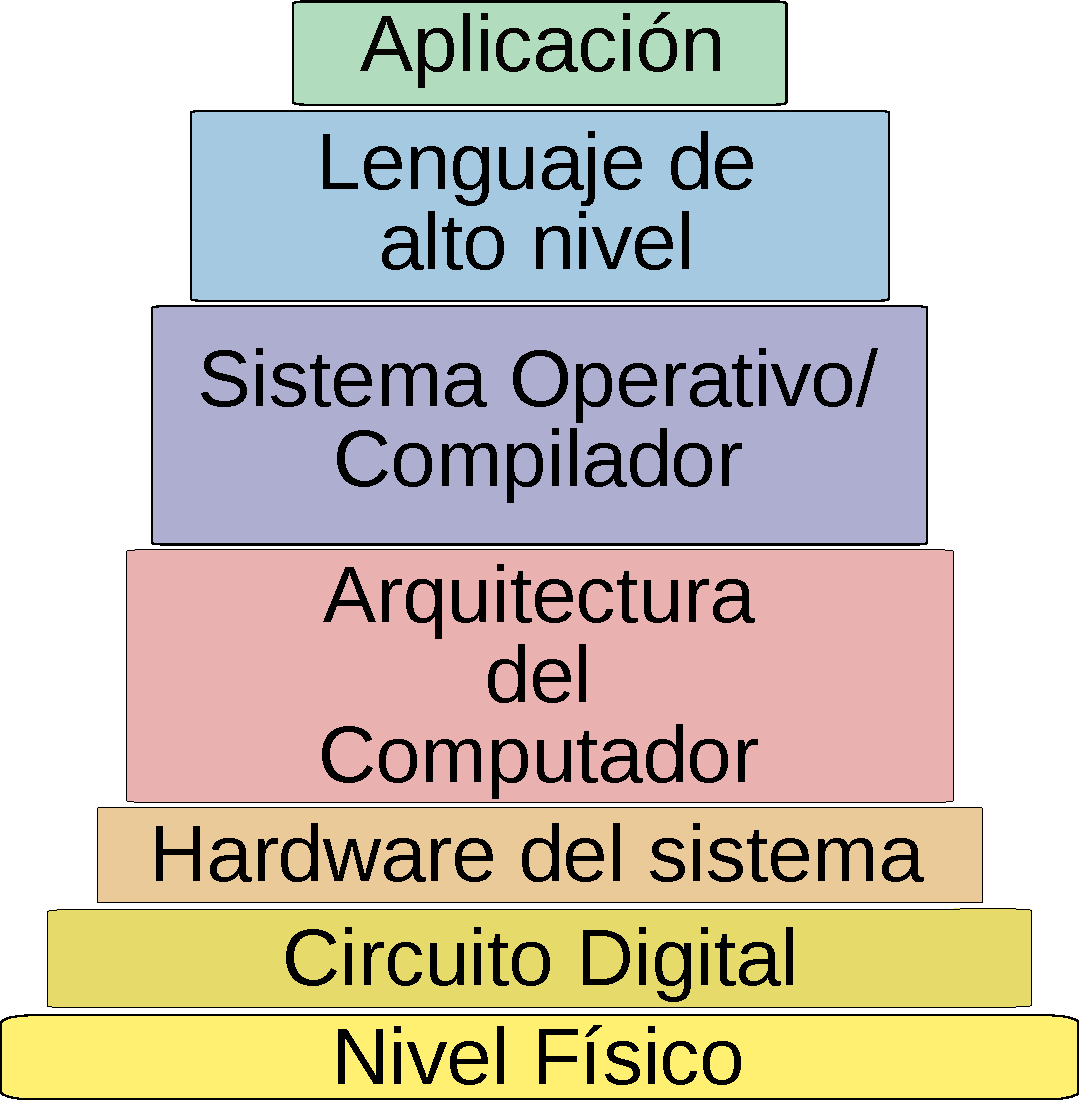
\includegraphics[width=10cm]{nivel_descripcion.pdf}
	\caption{Descripci�n por niveles de un computador}
	\label{fig:nivel}
\end{figure}
\begin{enumerate}
\item \textbf{Nivel F�sico.} Constituye la base del \emph{hardware} del computador. Est� constituido por los componentes electr�nicos b�sicos, diodos, transistores, resistencias, etc.  En un computador moderno, no es posible separar o tan siquiera observar dichos componentes: Se han fabricado directamente sobre un cristal semiconductor, y forman parte de un dispositivo electr�nico conocido con el nombre de circuito integrado.

\item \textbf{Circuito Digital.}
Los componentes del nivel f�sico se agrupan formando circuitos digitales, (En nuestro caso circuitos digitales integrados). Los circuitos digitales trabajan solo con dos niveles de tensi�n ($V_1, V_0$) lo que permite emplearlos para establecer relaciones l�gicas: $V_1$=verdadero, $V_2$=falso. Estas relaciones l�gicas establecidas empleando los valores de la tensi�n de los circuitos digitales constituyen el soporte de todos los c�lculos que el computador puede realizar.

\item \textbf{Organizaci�n Hardware del sistema.}\index{Computador ! \emph{hardware}} 
Los circuitos digitales integrados se agrupan y organizan para formar el \emph{Hardware} del ordenador.  Los m�dulos b�sicos que constituyen el \emph{Hardware} son la unidad central de procesos (CPU), La unidad de memoria y las unidades de entrada y salida de datos. Dichos componentes est�n conectados entre s� mediante un bus, que transfiere datos de una unidad a otra.

\item \textbf{Arquitectura del computador.} \index{Computador ! arquitectura}
La arquitectura define c�mo trabaja el computador. Por tanto, est� estrechamente relacionada con la organizaci�n hardware del sistema, pero opera a un nivel de abstracci�n superior. Establece c�mo se accede a los registros de memoria, arbitra el uso de los buses que comunican unos componentes con otros, y regula el trabajo de la CPU.  

Sobre la arquitectura se establece el lenguaje b�sico en el que trabaja el ordenador, conocido c�mo lenguaje m�quina. Es un lenguaje que emplea todav�a niveles l�gicos binarios (ceros o unos) y por tanto no demasiado apto para ser interpretado por los seres humanos. Este lenguaje permite al ordenador realizar operaciones b�sicas como copiar el contenido de un registro de memoria en otro, sumar el contenido de dos registros de memoria, etc. 

El lenguaje m�quina es adecuado para los computadores, pero no para los humanos, por eso, los fabricantes suministran junto con el computador un repertorio b�sico de instrucciones que su m�quina puede entender y realizar en un lenguaje algo m�s asequible. Se trata del lenguaje ensamblador. Los comandos de �ste lenguaje son f�cilmente traducibles en una o varias instrucciones de lenguaje m�quina.   A�n as� se trata de un lenguaje en el que programar directamente resulta una tarea tediosa y proclive a cometer errores. 

\item \textbf{Compiladores y Sistemas Operativos} \index{Sistema operativo} \index{Compilador}
Los Compiladores constituyen un tipo de programas especiales que permiten convertir un conjunto de instrucciones, escritas en un lenguaje de alto nivel en lenguaje m�quina. El programador escribe sus instrucciones en un fichero de texto normal, perfectamente legible para el ser humano, y el compilador convierte las instrucciones contenidas en dicho fichero en secuencias binarias comprensibles por la m�quina.

Los computadores primitivos solo eran capaces de ejecutar un programa a la vez. A medida que se fueron fabricando ordenadores mas sofisticados, surgi� la idea de crear programas que se encargaran de las tareas b�sicas: gestionar el flujo de informaci�n, manejar perif�ricos, etc. Estos programas reciben el nombre de sistemas operativos. Los computadores modernos cargan al arrancar un sistema operativo que controla la ejecuci�n del resto de las aplicaciones. Ejemplos de sistemas operativos son DOS (Disk Operating System), Unix y su versi�n para ordenadores personales Linux.

\item \textbf{Lenguajes de alto nivel.} \index{Programaci�n! lenguajes}
Los lenguajes de alto nivel est�n pensados para facilitar la tarea del programador, desentendi�ndose de los detalles de implementaci�n del hardware del ordenador.  Est�n compuestos por un conjunto de comandos y unas reglas sint�cticas, que permiten describir las instrucciones para el computador en forma de texto.

De una manera muy general, se pueden dividir los lenguajes de alto nivel en lenguajes compilados y lenguajes interpretados. Los lenguajes compilados emplean un compilador para convertir los comandos del lenguaje de alto nivel en lenguaje m�quina. Ejemplos de lenguajes compilados son C , C++ y Fortran. Los lenguajes interpretados a diferencia de los anteriores no se traducen a lenguaje m�quina antes de ejecutarse. Si no que utilizan otro programa --el interprete-- que va leyendo los comandos del lenguaje y convirti�ndolos en instrucciones m�quina a la vez que el programa se va ejecutando. Ejemplos de programas interpretado son Basic, Python y Java.

\item \textbf{Aplicaciones.} \index{Programaci�n! aplicaciones} Se suele entender por aplicaciones programas orientados a tareas espec�ficas, disponibles para un usuario final. Habitualmente se trata de programas escritos en un lenguaje de alto nivel y presentados en un formato f�cilmente comprensible para quien los usa.

Existen multitud de aplicaciones, entre las m�s conocidas cabe incluir los navegadores para Internet, como Explorer, Mocilla o Google Crome, los editores de texto, como Word, las hojas de c�lculo como Excel o los clientes de correo como Outlook. En realidad, la lista de aplicaciones disponibles en el mercado ser�a interminable. 
\end{enumerate}
\subsection{El modelo de computador de Von Neumann} \index{Von Neumann}
Los computadores modernos siguen, en lineas generales, el modelo propuesto por Von Newmann.  La figura \ref{fig:vonn} muestra un esquema de dicho modelo. 

\begin{figure}[h]
	\centering
		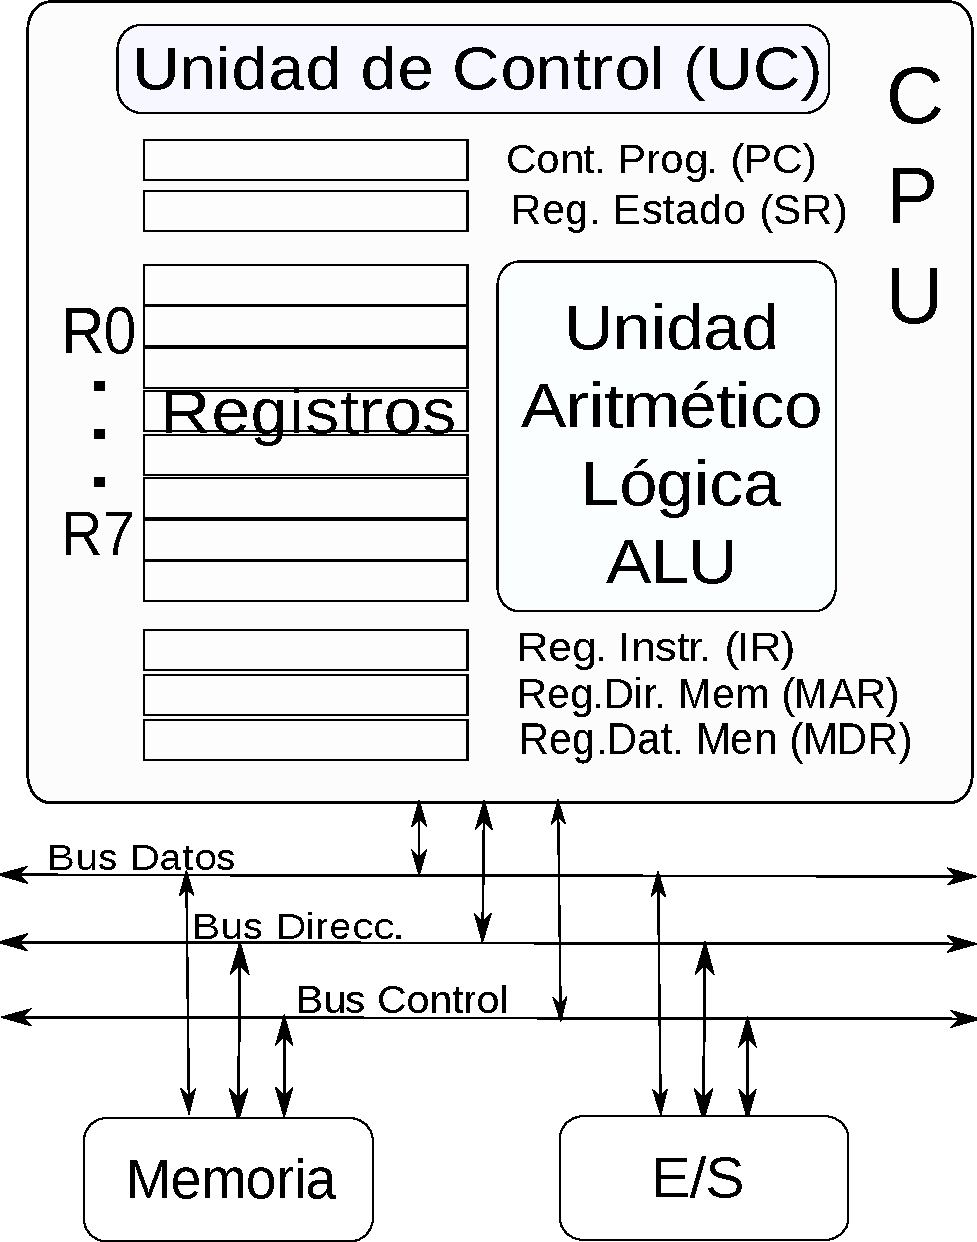
\includegraphics[width=10cm]{von.pdf}
	\caption{Modelo de Von Neumann}
	\label{fig:vonn}
\end{figure}

En el modelo de Von Newman se pueden  distinguir tres m�dulos b�sicos y una serie de elementos de interconexi�n.  Los m�dulos b�sicos son: 

\begin{itemize}
\item \textbf{La Unidad Central de Procesos.} CPU \index{CPU} (\emph{Central process unit)}) , esta unidad constituye el n�cleo en el que el ordenador realiza las operaciones. 

Dentro de la CPU pueden a su vez distinguirse las siguientes partes

\begin{itemize}

\item La unidad de proceso � ruta de datos: Est� formada por La Unidad Aritm�tico L�gica (ALU), \index{ALU} capaz de realizar las operaciones aritm�ticas y l�gicas que indican las instrucciones del programa. En general las ALUs se construyen para realizar aritm�tica entre enteros, y realizar las operaciones l�gicas b�sicas del algebra de Boole (AND, OR, etc). Habitualmente, las operaciones para n�meros no enteros, representados en \emph{punto flotante} se suelen realizar empleando un procesador espec�fico que se conoce con el nombre de Coprocesador matem�tico. La velocidad de procesamiento suele medirse en millones de operaciones por segundo (MIPS) o millones de operaciones en punto flotante por segundo (MFLOPS).

\item El banco de registros: Conjunto de registros en los que se almacenan los datos con los que trabaja la ALU y los resultados obtenidos.
 
\item La unidad de control (UC) o ruta de control: se encarga de buscar las instrucciones en la memoria principal y guardarlas en el registro de instrucciones, las decodifica, las ejecuta empleando la ALU, guarda los resultados en el registro de datos, y guarda las condiciones derivadas de la operaci�n realizada en el registro de estado.  El registro de datos de memoria, contiene los datos que se est�n leyendo de la memoria principal o van a escribirse en la misma. El registro de direcciones de memoria, guarda la direcci�n de la memoria principal a las que esta accediendo la ALU, para leer o escribir. El contador del programa, tambi�n conocido como puntero de instrucciones, es un registro que guarda la posici�n en la que se encuentra la CPU dentro de la secuencia de instrucciones de un programa.
\end{itemize}
 

\item \textbf{La unidad de memoria.} Se trata de la memoria principal o primaria del computador.  Est� dividida en bloques de memoria que se identifican mediante una direcci�n. La CPU tiene acceso directo a dichos bloques de memoria.

La unidad elemental de informaci�n digital es el bit \index{bit} (0,1). La capacidad de almacenamiento de datos se mide en Bytes \index{Byte} y en sus m�ltiplos, calculados  como potencias de 2\footnote{Los prefijos $K$(Kilo),$M$(Mega),$G$ (Giga), etc., se reservan en el sistema internacional para indicar potencias de 10. Para su equivalente en potencias de 2 se deben emplear los t�rminos $Ki$ (Kibi), $Mi$ (Mebi),$Gi$ (Gibi),$Ti$,(Tebi). Por tanto, deber�a decirse  Kibibyte, Mebibyte, etc. Sin embargo, esta notaci�n no est� muy extendida y se habla de KB (KiloBytes), MB (Megabytes), etc aunque se realice el c�lculo en potencias de 2 }

\begin{align} \nonumber
1\  Byte = &\ 8\ bits\ &\  \\ \nonumber
1\  Word = &\ 16\ bits=2B &\  \\ \nonumber
1\  KiB  = &\ 2^{10}\ bits=1024\ B&\ \\  \nonumber
1\  MiB = &\ 2^{20}\ bits=1024\ KB&\ \\  \nonumber
1\  GiB = &\ 2^{30}\ bits &\ \\  \nonumber
1\  TiB  = &\ 2^{40}\ bits\ &\
\end{align} 

\item \textbf{Unidad de Entrada/Salida.} Transfiere informaci�n entre el computador y los dispositivos perif�ricos.
\end{itemize}

Los elementos de interconexi�n se conocen con el nombre de \emph{Buses}. Se pueden distinguir tres: En bus de datos, por el que se transfieren datos entre la CPU y la memoria � la unidad de entrada/salida. El bus de direcciones, par especificar una direcci�n de memoria o del registro de E/S. Y el bus de Control, por el que se env�an se�ales de control, tales como la se�al de reloj, la se�al de control de lectura/escrituras entre otras.  

\subsection{Representaci�n binaria} \index{Base 2}
Veamos con algo m�s de detalle, c�mo representa la informaci�n un computador. Como se explic� anteriormente, La electr�nica que constituye la parte f�sica del ordenador, trabaja con dos niveles de voltaje. Esto permite definir dos estados, --alto, bajo-- que pueden representarse dos s�mbolos  $0$ y $1$. Habitualmente, empleamos $10$ s�mbolos ${0,1,2,3,4,5,6,7,8,9}$, es decir, empleamos una representaci�n decimal. Cuando queremos representar n�meros mayores que nueve, dado que hemos agotado el n�mero de d�gitos disponibles, lo que hacemos es combinarlos, agrupando cantidades de diez en diez. As� por ejemplo, el numero $16$, representa seis unidades m�s un grupo de diez unidades y el n�mero $462$ representa dos unidades m�s seis grupos de diez unidades m�s cuatro grupos de 10 grupos de 10 unidades.  Matem�ticamente, esto es equivalentes a emplear sumas de d�gitos por potencias de diez:
\begin{equation*}
13024 = 1\times10^4+3\times10^3+0\times10^2+2\times10^1+4\times10^0 
\end{equation*}

Si recorremos los d�gitos que componen el n�mero de izquierda derecha, cada uno de ellos representa una potencia de diez superior, porque cada uno representa la cantidad de grupos de 10 grupos, de grupos ... de diez grupos de unidades. Esto hace que potencialmente podamos representar cantidades tan grandes como queramos, empleando tan solo diez s�mbolos. Esta representaci�n, a la que estamos habituados recibe el nombre de representaci�n en base 10 \index{Base 10}. Pero no es la �nica posible.

Volvamos a la representaci�n empleada por el computador. En este caso solo tenemos dos s�mbolos distintos el $0$ y el $1$. Si queremos emplear una representaci�n an�loga a la representaci�n en base diez, deberemos agrupar ahora las cantidad en grupos de dos. As� los �nicos n�meros que admiten ser representados con un solo d�gito son el uno y el cero. Para representar el n�mero dos, necesitamos agrupar: tendremos $0$ unidades y $1$ grupo de dos, con lo que la representaci�n del n�mero dos en base dos ser� $10$. Para representar el n�mero tres, tendremos una unidad m�s un grupo de dos, por lo que la representaci�n ser� $11$, y as� sucesivamente. Matem�ticamente esto es equivalente emplear sumas de d�gitos por potencias de 2:

\begin{equation*}
10110 = 1\times2^4+0\times2^3+1\times2^2+1\times2^1+0\times2^0 
\end{equation*}

Esta representaci�n recibe el nombre de representaci�n binaria o en base 2.
\index{Conversi�n! binario a decimal}La expansi�n de un n�mero representado en binario en potencias de 2, nos da un m�todo directo de obtener su representaci�n decimal. As�, para el ejemplo anterior, si calculamos las potencias de dos y sumamos los resultados obtenemos:

  \begin{equation*}
  1\times2^4+0\times2^3+1\times2^2+1\times2^1+0\times2^0=16+0+4+2+0=22 
\end{equation*}

que es la representaci�n en base 10 del n�mero binario $10110$.

Para n�meros no enteros, la representaci�n tanto en decimal como en binario, se extiende de modo natural empleando potencias negativas de 10 y de 2 respectivamente. As�,
 
\begin{equation} \nonumber
835.41 = 8\times10^2+3\times10^1+5\times10^0+4\times10^{-1}+1\times10^{-2} 
\end{equation}

y para un n�mero en binario,

\begin{equation} \nonumber
101.01 = 1\times2^2+0\times2^1+1\times2^0+0\times2^{-1}+1\times2^{-2} 
\end{equation}

De nuevo, basta calcular el t�rmino de la derecha de la expresi�n anterior para obtener la representaci�n decimal del n�mero $101.01$.

\index{Conversi�n! decimal a binario. n�meros enteros}�C�mo transformar la representaci�n de un n�mero de decimal a binario? De nuevo nos da la clave la representaci�n en sumas de productos de d�gitos por potencias de dos. Empecemos por el caso de un n�mero entero. Supongamos un n�mero D, representado en decimal. Queremos expandirlo en una suma de potencias de dos. Si dividimos el n�mero por 2, podr�amos representarlo c�mo:
 
\begin{equation*}
\label{eq:1}
D=2\cdot C_1+R_1
\end{equation*}

donde $C_1$ representa el cociente de la divisi�n y $R_1$ el resto. Como estamos dividiendo por dos, el resto solo puede valer cero o uno. Supongamos ahora que volvemos a dividir el cociente obtenido por dos,

 \begin{equation*}
 \label{eq:2}
C_1=2\cdot C_2+R_2 \
\end{equation*}

Si sustituimos el valor obtenido para $C_1$ en la ecuaci�n inicial obtenemos,   
\begin{equation*}
D=2\cdot(2\cdot C_2+R_2)+R_1= 2^2\cdot C_2+R_2\cdot 2^1+R_1\cdot 2^0 
\end{equation*}

Si volvemos a dividir el nuevo cociente obtenido $C_2$ por dos, y volvemos a sustituir,

 \begin{align*}
C_2&=2\cdot C_3+R_3 \\
D&=2^2\cdot(2\cdot C_3+R_3)+R_2\cdot 2^1+R_1\cdot 2^0=2^3\cdot C_3+R_3\cdot 2^2 +R_2\cdot 2^1+R_1\cdot 2^0
\end{align*}

Supongamos que tras repetir este proceso $n$ veces, obtenemos un conciente $C_n=1$. L�gicamente no tiene sentido seguir dividiendo ya que a partir de este punto, cualquier divisi�n posterior que hagamos nos dar� cociente $0$ y resto igual a $C_n$. Por tanto, 

 \begin{align*}
D&=1\cdot 2^n+R_n\cdot 2^{n-1}\cdots +R_3\cdot 2^2 +R_2\cdot 2^1+R_1\cdot 2^0
\end{align*}

La expresi�n obtenida, coincide precisamente con la expansi�n en potencias de dos del n�mero binario $1R_n \cdots R_3R_2R_1$.


Como ejemplo,podemos obtener la representaci�n en binario del n�mero $234$, empleando el m�todo descrito: vamos dividiendo el n�mero y los cocientes sucesivos entre dos, hasta obtener un cociente igual a uno y a continuaci�n, construimos la representaci�n binaria del n�mero colocando por orden, de derecha a izquierda.  los restos  obtenidos de las sucesivas divisiones y a�adiendo un uno m�s a la izquierda de la cifra construida con los restos:

\begin{table}[h]
\begin{tabular}{|r|r|r|r|}
Dividendo& &Cociente $\div 2$&Resto\\
\hline
234& &117&0\\
117& &58&1\\
58& &29&0\\
29& &14&1\\
14& &7&0\\
7& &3&1\\
3& &1&1
\end{tabular}
\end{table}
 
 Por tanto, la representaci�n en binario de 234 es 11101010.
 
\index{Conversi�n! decimal a binario, n�meros no entero}Supongamos ahora un n�mero no entero, representado en decimal, de la forma $0,d$ . Si lo multiplicamos por dos:

\begin{equation}
E_1,d_1=0,d\cdot 2
\end{equation}
Donde $E_1$ representa la parte entera y $d_1$ la parte decimal del n�mero calculado.
Podemos entonces representar $0,d$ como,
\begin{equation}
\label{eq:5}
0,d=(E_1,d_1)\cdot 2^{-1}=E_1\cdot 2^{-1}+0,d_1\cdot 2^{-1}
\end{equation}  

Si volvemos a multiplicar $0,d_1$ por dos,

\begin{equation}
E_2,d_2 = 0,d_1\cdot 2
\end{equation}

\begin{equation}
0,d_1=E_2\cdot 2^{-1}+0,d_2\cdot 2^{-1}
\end{equation}  

y sustituyendo en \ref{eq:5}

\begin{equation}
0,d=E_1\cdot 2^{-1}+E_2\cdot 2^{-2}+0,d_2\cdot 2^{-2}
\end{equation}

�Hasta cuando repetir el proceso? En principio hasta que obtengamos un valor cero para la parte decimal, $0,d_n=0$. Pero esta condici�n puede no cumplirse nunca. Puede darse el caso --de hecho es lo m�s probable-- de que un n�mero que tiene una representaci�n exacta en decimal, no la tenga en binario. El criterio para detener el proceso ser� entonces obtener un determinado n�mero de decimales o bien seguir el proceso hasta que la parte decimal obtenida vuelva a repetirse. Puesto que los ordenadores tienen un tama�o de registro limitado, tambi�n est� limitado el n�mero de d�gitos con el que pueden representar un n�mero decimal. Por eso, lo habitual ser� truncar el n�mero asumiendo el error que se comete al proceder as�.  De este modo, obtenemos la expansi�n del n�mero original en potencias de dos,

\begin{equation}
0,d\cdot 2=E_1\cdot 2^{-1}+E_2\cdot 2^{-2}+\cdots+ E_n\cdot 2^{-3}+\cdots
\end{equation} 

Donde los valores $E_1\cdots E_n$ son precisamente los d�gitos correspondientes a la representaci�n del n�mero en binario: $0.E_1E_2\cdots E_n$. (Es trivial comprobar que solo pueden valer $0$ � $1$).


Veamos un ejemplo de cada caso, obteniendo la representaci�n binaria del n�mero $0,625$, que tiene representaci�n exacta, y la del n�mero $0,626$, que no la tiene. En este segundo caso, calcularemos una representaci�n aproximada, tomando 8 decimales.

\begin{table}[h]
\begin{tabular}{|r|r|r|r|r r|r|r|r|r|}
P decimal& &$\times 2$& P entera& &&P decimal& &$\times 2$& P entera\\
\cline{1-4}
\cline{7-10}
0,625& &1,25&1& &&0,623& &1,246&1\\
0,25  & &0,5  &0& &&0,246& &0,492&0\\
0,5    & &1,0  &1& &&0,492& &0,984&0\\
         & &       &  & &&0,984& &1,968&1\\
         & &       &  & &&0,968& &1,936&1\\
         & &       &  & &&0,936& &1,872&1\\
         & &       &  & &&0.872& &1.744&1\\
         & &       &  & &&0.744& &1.488&1\\
\end{tabular}
\end{table}

Para construir la representaci�n binaria del primero de los n�meros, nos basta tomar las partes enteras obtenidas, por orden, escribirlas de de izquierda a derecha y a�adir un $0$ y la coma decimal a la izquierda. Por tanto  la representaci�n binaria de $0,625$ es $0,101$.  Si expandimos su valor en potencias de dos, volvemos a recuperar el n�mero original en su representaci�n decimal.

 En el segundo caso, la representaci�n binaria, tomando nueve decimales de $0,623$ es $0.10011111$. Podemos calcular el error que cometemos al despreciar el resto de los decimales, volviendo a convertir el resultado obtenido a su representaci�n en base diez,

 \begin{equation*}
0\cdot 2^{0}+1\cdot 2^{-1}+0\cdot 2^{-2}+ 0\cdot 2^{-3}+1\cdot 2^{-4}+1\cdot 2^{-5}+ 1\cdot 2^{-6}+1\cdot 2^{-7}+1\cdot 2^{-8}=0,62109375
\end{equation*} 

El error cometido es, en este caso: $\text{Error}=0,623-0,62109375=0,00190625$.
  
 \section{Aplicaciones de Software Cient�fico}
Dentro del mundo de las aplicaciones, merecen una menci�n aparte las dedicadas al c�lculo cient�fico, por su conexi�n con la asignatura. 

Es posible emplear lenguajes de alto nivel para construir rutinas y programas que permitan resolver directamente un determinado problema de c�lculo. En este sentido, el lenguaje FORTRAN se ha empleado durante a�os para ese fin, y todav�a sigue emple�ndose en muchas disciplinas cient�ficas y de la Ingenier�a.  Sin embargo, hay muchos aspectos no triviales del c�lculo con un computador, que obligar�an al cient�fico que tuviera que programar sus propios programas a ser a la vez un experto en computadores.  Por esta raz�n, se han ido desarrollando aplicaciones espec�ficas para c�lculo cient�fico que permiten al investigador centrarse en la resoluci�n de su problema y no en el desarrollo de la herramienta adecuada para resolverlo.  
 
En algunos casos, se trata de aplicaciones a medida, relacionadas directamente con alg�n �rea cient�fica concreta. En otros, consisten en paquetes de funciones espec�ficos para realizar de forma eficiente determinados c�lculos, como por ejemplo
el paquete SPSS para c�lculo estad�stico.

Un grupo especialmente interesante lo forman algunos paquetes de software que podr�amos situar a mitad de camino entre los lenguajes de alto nivel y las aplicaciones: Contienen extensas librer�as de funciones, que pueden ser empleadas de una forma directa para realizar c�lculos y adem�s permiten realizar programas espec�ficos empleando su propio lenguaje. Entre estos podemos destacar Mathematica, Maple , Matlab, Octave y Scilab y Python. El uso de estas herramientas se ha extendido enormemente en la comunidad cient�fica. Algunas como Matlab  constituyen casi un est�ndar en determinadas �reas de conocimiento.

 


    

 

  

\chapter{Introducci�n a la programaci�n en Matlab} \index{Matlab}
Este cap�tulo presenta una introducci�n general a la programaci�n. Para su desarrollo, vamos a emplear una de las aplicaciones inform�ticas para c�lculo cient�fico que m�s aceptaci�n ha tenido en los �ltimos a�os: el entorno de programaci�n de Matlab. Matlab es el acr�nimo de MATrix LABboratory. El nombre est� relacionado con el empleo de matrices como elemento b�sico para el c�lculo num�rico.

Usaremos esta herramienta, entre otras motivos, porque nos ofrece la posibilidad de realizar programas similares a los que podr�amos desarrollar con un lenguaje de programaci�n de alto nivel, nos permite resolver problemas de c�lculo cient�fico directamente, empleando las herramientas que incluye y, adem�s, nos permite combinar ambas cosas.

Este cap�tulo no pretende ser exhaustivo, --cosa que por otro lado resulta imposible en el caso de Matlab--, sino tan solo dar una breve introducci�n a su uso. Afortunadamente, Matlab cuenta con una muy buena documentaci�n, accesible a trav�s de la 'ayuda', eso s�, en ingl�s. 



\section{El entorno de programaci�n de Matlab}\index{Matlab! entorno de programaci�n}\index{Matlab! IDE}
Cuando iniciamos Matlab en el computador, se abre una ventana formada por uno o m�s paneles. Esta ventana, constituye lo que en programaci�n se  llama un entorno de desarrollo integrado o, abreviadamente, IDE (acr�nimo tomado de su nombre en Ingl�s: \emph{integrated development environment}. El IDE de Matlab, contiene todo los elementos necesarios para programar. La figura \ref{fig:ide} muestra el aspecto del IDE de Matlab.

\begin{figure}[h]
	\centering
		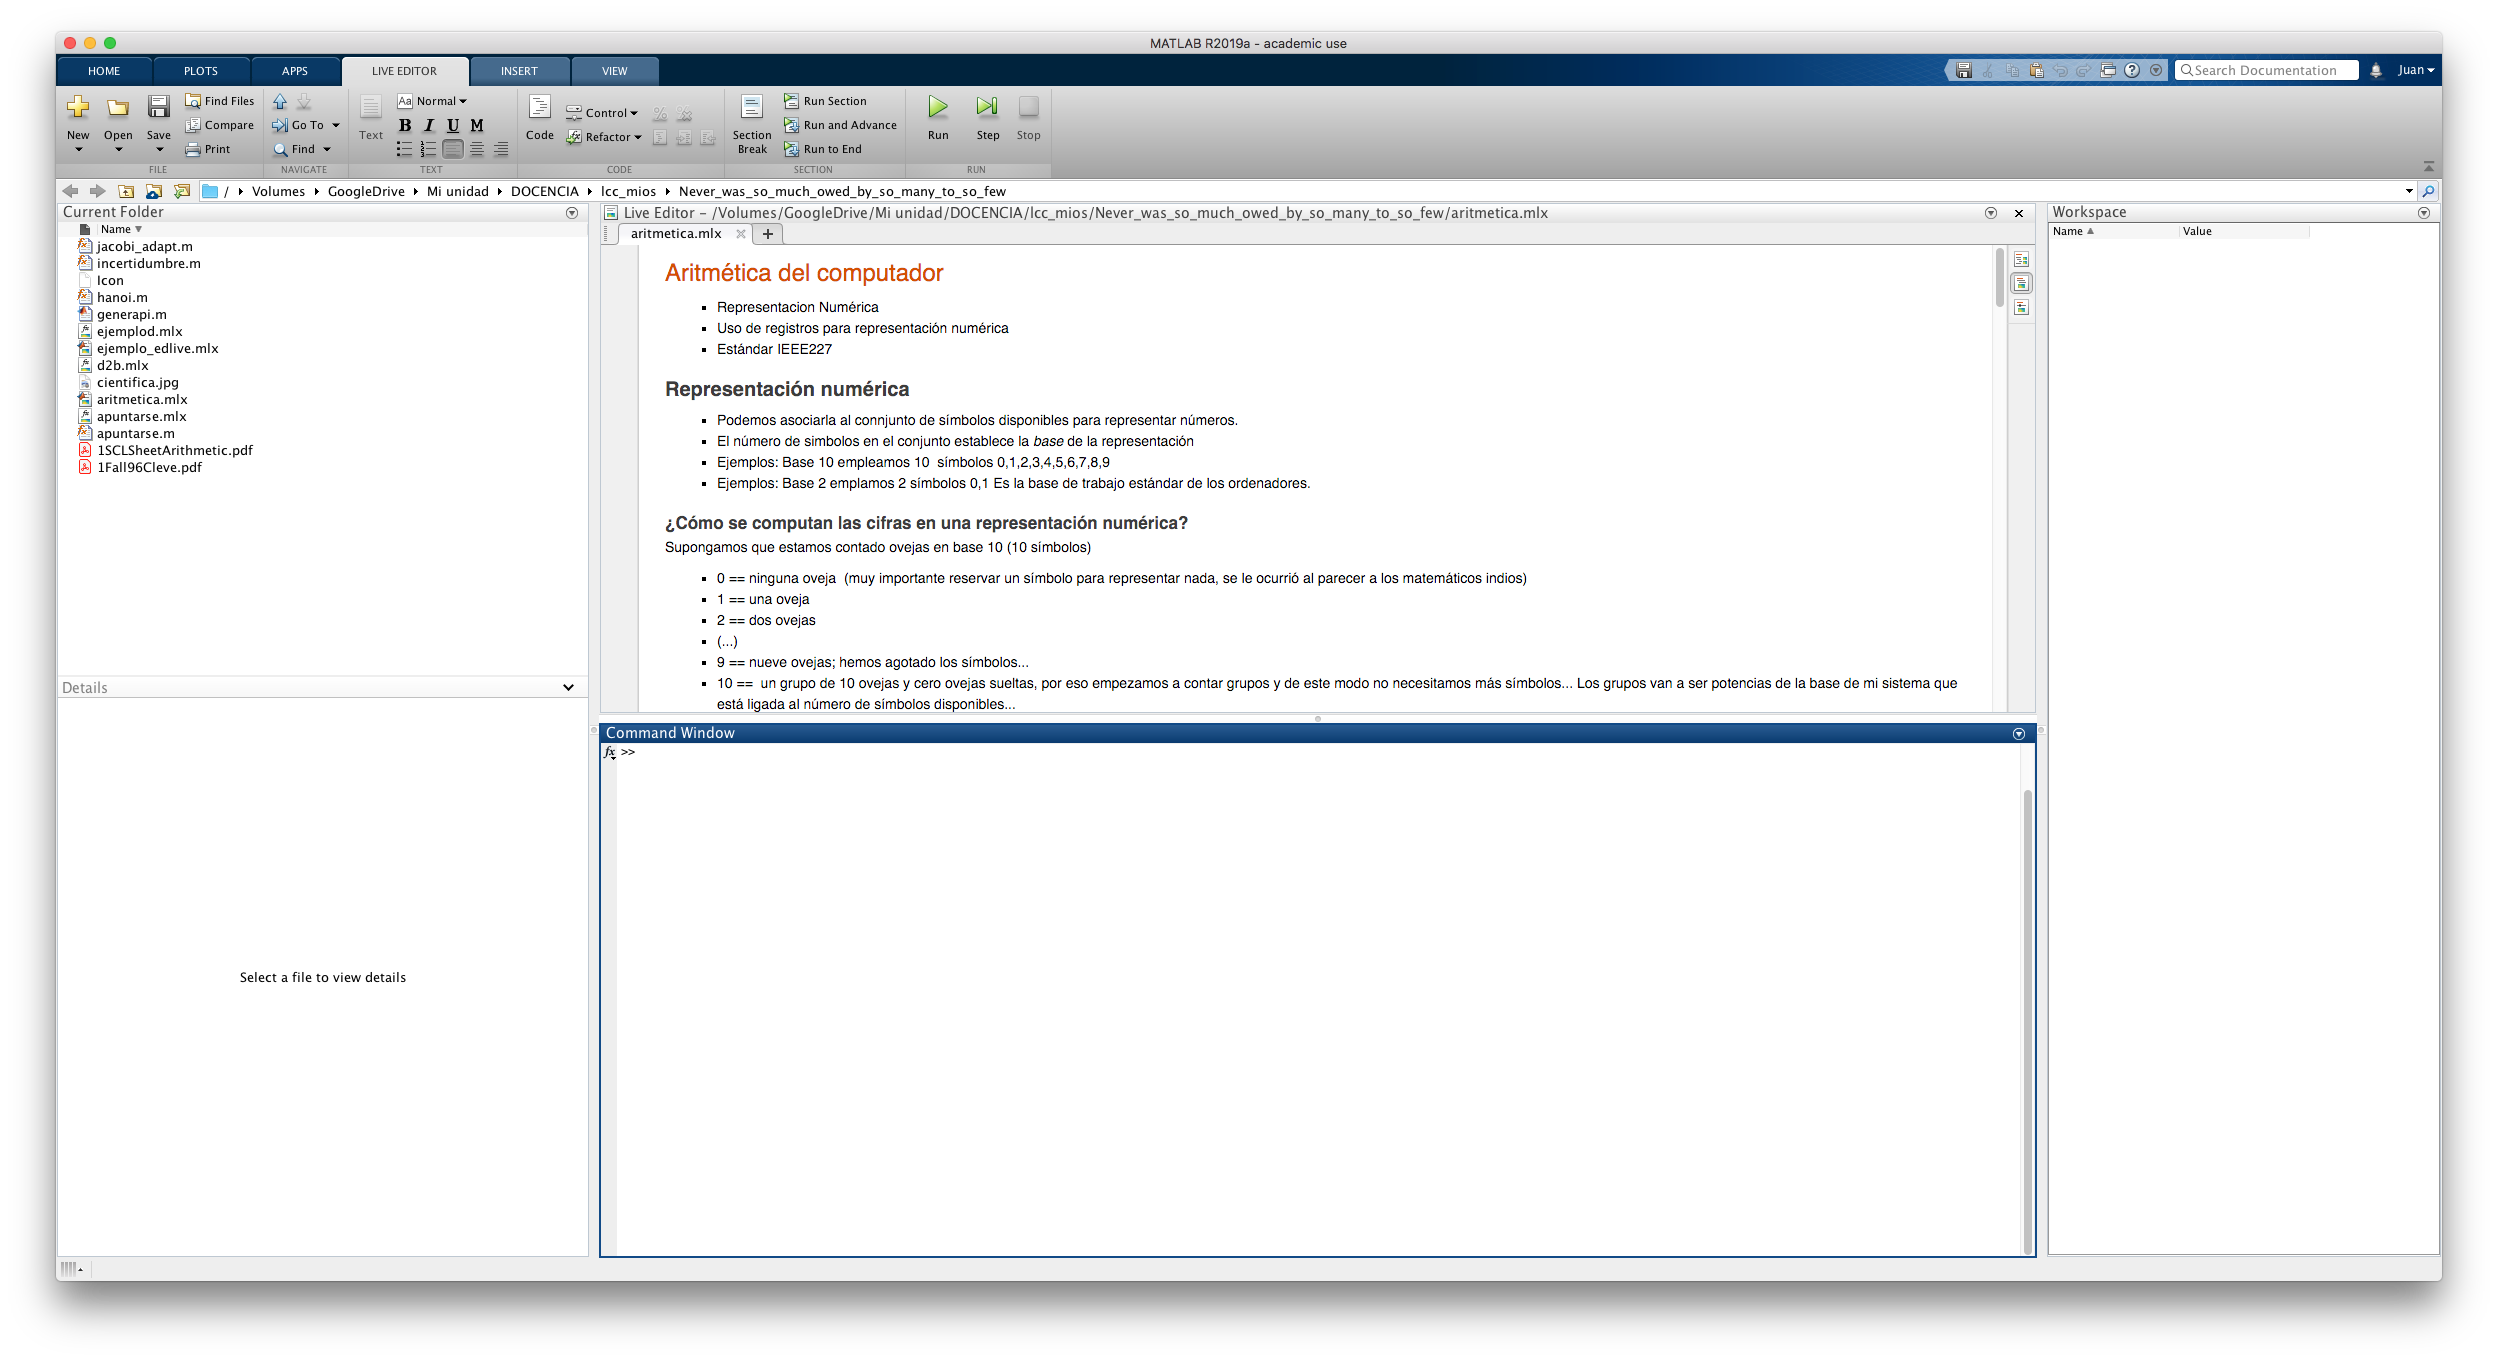
\includegraphics[width=14cm]{ide_n.png}
	\caption{Entorno de desarrollo integrado de Matlab}
	\label{fig:ide}
\end{figure}

Seg�n como se configure, el IDE de Matlab puede mostrar un n�mero mayor o menor de paneles y una disposici�n de los mismos distinta a la mostrada en la figura. La mejor manera de aprender estos y otros detalles del IDE es usarlo. Aqu� nos centraremos solo en algunos aspectos fundamentales.

\subsection{La ventana de comandos de Matlab} \index{Matlab!ventana de Commandos}
De los paneles mostrados en la ventana de la figura \ref{fig:ide}, vamos a empezar examinando el situado en la parte inferior central. Se trata de la ventana de comandos (\emph{command window}) de Matlab.  \index{prompt} La ventana muestra el simbolo $>>$, que recibe el nombre de \emph{prompt} y, a continuaci�n, una barra vertical $|$ parpadeante.  La ventana de comandos permite al usuario interactuar directamente con Matlab: Matlab puede recibir instrucciones directamente a trav�s de la ventana de comandos, ejecuta las instrucciones recibidas, y devuelve los resultados de nuevo en la ventana de comandos. Veamos un ejemplo muy sencillo: si escribimos en la ventana de comandos:

\begin{verbatim}
>> a=18 + 3
\end{verbatim}

Matlab calcula la suma pedida, devuelve el resultado y, por �ltimo, vuelve a presentar el \emph{prompt}, para indicarnos que est� preparado para recibir otro comando.

\begin{verbatim}
a =

    21

>> 
\end{verbatim}

De este modo, podemos emplear Matlab de un modo an�logo a como emplear�amos una calculadora: realizamos una operaci�n, obtenemos el resultado, realizamos otra operaci�n, obtenemos el resultado  y as� sucesivamente.
\subsection{Variables.} \index{Variable}
En el el ejemplo que acabamos de ver, Matlab calcula el resultado pedido, y lo presenta en pantalla usando la expresi�n, \begin{verbatim}
a =21
\end{verbatim} �Por qu� hace falta escribir $a=18+3$ en lugar de escribir directamente $18+3$? La raz�n tiene que ver con el modo de trabajo de Matlab, y de otros lenguajes de alto nivel. Esto nos lleva al concepto de variable. 

Podemos ver una variable como una regi�n de la memoria del computador, donde un programa guarda una determina informaci�n; n�meros, letras, etc. Una caracter�stica fundamenta de una variable es su nombre, ya que permite identificarla. \index{Variable! nombre} Como nombre para una variable se puede escoger cualquier combinaci�n de letras y n�meros, empezando siempre con una letra, en el caso de Matlab\footnote{Como se ver� m�s adelante, Matlab tiene un conjunto de nombres de instrucciones y comandos ya definidos. Se debe evitar emplear dichos nombres, ya que de hacerlo se pierde acceso al comando de Matlab que representan}. Se puede adem�s emplear el signo "\_". Matlab distingue entre may�sculas y min�sculas, por lo que si elegimos como nombres de variable Pino, PINO y PiNo, Matlab las considerar� como variables distintas. 

\index{Variable! tipo} En algunos lenguajes, es preciso indicar al ordenador qu� tipo de informaci�n se guardar� en una determinada variable, antes de poder emplearlas. Esto permite manejar la memoria del computador de una manera m�s eficiente, asignando zonas adecuadas a cada variable, en funci�n del tama�o de la informaci�n que guardar�n. A este proceso, se le conoce con el nombre de \emph{declaraci�n} de variables. En Matlab no es necesario declarar las variables antes de emplearlas.

El m�todo m�s elemental de emplear una variable es asignarle la informaci�n para la que se cre�. Para hacerlo, se emplea el s�mbolo de asignaci�n \index{"= S�mbolo de asignaci�n} \index{S�mbolo de asignaci�n}, que coincide con el signo $=$ empleado en matem�ticas. Como veremos m�s adelante la asignaci�n en programaci�n y la igualdad en matem�ticas no representan ex�ctamente lo mismo. La manera de asignar directamente informaci�n a una variable es escribir el nombre de la variable, a continuaci�n  el signo de asignaci�n y, por �ltimo, la informaci�n asignada,
\begin{verbatim}
Nombre_variable = 4
\end{verbatim}  

Si escribimos en la ventana de comandos la expresi�n anterior y pulsamos el retorno de carro. Matlab devuelve el siguiente resultado:

\begin{verbatim}
>> Nombre_variable=4

Nombre_variable =

     4

>> 
\end{verbatim}  
Matlab ejecuta las instrucciones indicadas y nos confirma que ha creado en la memoria una variable \texttt{Nombre\_variable} y que ha guardado en  ella el n�mero $4$. 

En Matlab podemos emplear el s�mbolo de asignaci�n para construir variables que guarden distintos tipos de datos,

\begin{enumerate}
\item Enteros positivos y negativos
\begin{verbatim}
>> a=4
a =

     4

>>b=-4
b =

     -4

\end{verbatim}
\item N�meros con parte entera y parte decimal separadas por un punto, positivos y negativos.
\begin{verbatim}
>> a=13.4568
a =

   13.4568

>> b=-13.4568
b =

   -13.4568
\end{verbatim}


\item N�meros expresados como potencias de $10$ (la potencia de $10$ se representa con la letra e seguida del valor del exponente). 
\begin{verbatim}
>> f=3e10
f =

  3.0000e+010

>> g=-3e10
g =

 -3.0000e+010

>> h=3e-10
h =

  3.0000e-010

>> t=-3e-10
t =

 -3.0000e-010
 \end{verbatim}
 
\item N�meros complejos. Para indicar la parte imaginaria se puede emplear la letra \texttt{i} o la letra \texttt{j}.

\begin{verbatim}
>> s=2+3i
s =

   2.0000 + 3.0000i

>> w=4-5j
w =

   4.0000 - 5.0000i
\end{verbatim}

\item Caracteres, letras o n�meros; manejados estos �ltimos como s�mbolos. Se indica a Matlab que se trata de un car�cter escribi�ndolo entre comillas simples,
\begin{verbatim}
>> p='a'
p =

a

>> k='1'
k =

1
\end{verbatim}

\item Cadenas de caracteres. 
\begin{verbatim}
>> m='hola amigos'
m =

hola amigos
\end{verbatim}

\end{enumerate}
 La forma que hemos visto de asignar un valor a una variable es la m�s sencilla pero no es la �nica. Tambi�n podemos asignar un valor a una variable a partir de una expresi�n aritm�tica, como hemos visto antes. Ademas podemos asignar un valor a una variable copiando el contenido de otra variable:
\begin{verbatim}
>> a=18

a =

    18

>> b=a

b =

    18

>> 
\end{verbatim}
Por �ltimo, podemos asignar a una variable el valor de una funci�n en un punto:
\begin{verbatim}
>> x=0
x =

     0

>> y=cos(x)
y =

     1

>> 
\end{verbatim}

La variable \texttt{y} contiene el valor de la funci�n coseno en el punto \texttt{x=0}. M�s adelante estudiaremos c�mo manejar funciones en Matlab. 

Si escribimos directamente en la l�nea de comandos de Matlab, un n�mero, una expresi�n algebraica o una funci�n, sin asignarlas a una variable, Matlab crea autom�ticamente una variable para guardar el resultado, As� por ejemplo:
\begin{verbatim}
>> 3 + 5
ans =

     8

>> 
\end{verbatim}
Matlab guarda el resultado de la operaci�n realizada: $3+5$, en la variable \texttt{ans}\index{ans, nombre de variable por defecto}.  Se trata del nombre de variable por defecto; es una abreviatura de al palabra inglesa \emph{answer} (respuesta).  En cualquier caso es recomendable asignar los resultados de las operaciones expl�citamente a una variable.  La raz�n para ello tiene que ver con lo que llamaremos reasignaci�n de variables.

Imaginemos que creamos en Matlab una variable asign�ndole un valor:

\begin{verbatim}
>> a=34

a =

    34

>> 
\end{verbatim}
Si a continuaci�n, asignamos a esa misma variable el resultado de una operaci�n,
\begin{verbatim}
>> a=12+5

a =

    17

>> 
\end{verbatim}
El valor inicialmente asignado a la variable \texttt{a} se pierde. Sencillamente hemos \emph{reasignado} a la variable un nuevo valor sobreescribiendo el anterior. Si en la l�nea de comandos escribimos operaciones sin asignar el resultado a una variable concreta, Matlab lo asignar� a la variable \texttt{ans} pero esto significa que cada nueva operaci�n reasigna su resultado a la variable \texttt{ans}, con lo que solo conservaremos al final el resultado de la �ltima de las operaciones realizadas.

Es posible en Matlab crear una variable que no contenga nada. Para ello hay que emplear dos s�mbolos especiales: $[$ y $]$. As�, si escribimos en la l�nea de comandos:
\begin{verbatim}
>> variable_vacia=[]

variable_vacia =

     []

>> 
\end{verbatim}
obtenemos una variable que no contiene nada. M�s adelante veremos la utilidad de hacerlo.

Hasta ahora, siempre que hemos realizado una operaci�n en la ventana de comandos, Matlab nos ha \emph{respondido} escribiendo en pantalla el resultado de la misma. En muchas ocasiones, no nos interesa que Matlab nos muestre por pantalla el resultado de una operaci�n; por ejemplo, porque se trata de un resultado intermedio, o porque es un resultado de gran tama�o y su visualizaci�n por pantalla no es �til y sin embargo s� que consume mucho tiempo. Podemos omitir la visualizaci�n por pantalla del resultado de una operaci�n, si terminamos la operaci�n, a�adiendo al final un \emph{punto y coma} (\texttt{;}),

\begin{verbatim}
>> A=3+5;
>> B=A+1
B =

     9

\end{verbatim}
En la primera operaci�n hemos a�adido (\texttt{;}) al final de la l�nea, Matlab no muestra el resultado. Sin embargo, s� que ha realizado la operaci�n pedida y guardado el resultado en la variable \texttt{A}. Por eso es posible emplearla en la segunda operaci�n para crear la variable \texttt{B}.
\paragraph*{Recursi�n.} \index{Recursi�n} Hemos indicado antes c�mo el s�mbolo de asignaci�n $=$ en programaci�n no coincide exactamente con la igualdad matem�tica. Un ejemplo claro de estas diferencias lo constituye la recursi�n. Esta se produce cuando la misma variable aparece a los dos lados del s�mbolo de asignaci�n:
\begin{verbatim}
>> a=3

a =

     3

>> a=a+1

a =

     4
\end{verbatim} 
La expresi�n anterior no tiene sentido matem�ticamente, ya que una variable no puede ser igual a s� misma m�s la unidad. Sin embargo, en programaci�n, es  una sentencia v�lida; el ordenador toma el valor almacenado en la variable $a$, le suma $1$ y guarda el resultado en la variable $a$, sobreescribiendo el valor anterior.

La recursi�n se emplea muy a menudo en programaci�n, entre otras aplicaciones, permite crear contadores, --variables que van incrementando o decrementando su valor progresivamente--  y permite ahorrar espacio de memoria cuando se realizan operaciones que requieren c�lculos intermedios.

\paragraph*{El espacio de trabajo de Matlab \emph{Workspace}.} \index{Workspace}\index{Espacio de trabajo} Matlab guarda en memoria las variables que creamos en la ventana de comandos y las asocia a lo que se conoce como el espacio de trabajo de Matlab. Dicho espacio de trabajo contiene una relaci�n de las variables creadas de modo que podamos volver a utilizarlas en la ventana de comandos. Uno de los paneles que el IDE de Matlab puede mostrarnos es precisamente el \emph{Workspace}. La figura \ref{fig:wsp} muestra dicho panel.  En el se muestran los nombres de las variables contenidas en el espacio de trabajo, as� como informaci�n relativa a su valor, tama�o en memoria etc.


\begin{figure}[h]
	\centering
		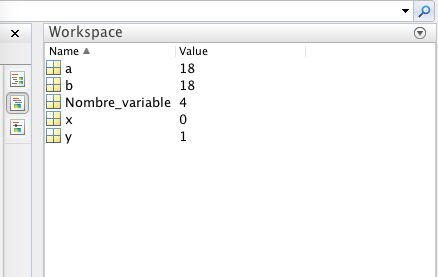
\includegraphics[width=8cm]{wsp2.png}
	\caption{El \emph{Workspace} de Matlab}
	\label{fig:wsp}
\end{figure}

Adem�s del panel que acabamos de describir, es posible listar el contenido de las variables presentes en el \emph{Workspace} empleando dos comandos especiales de Matlab; se trata de los comandos \texttt{who} y \texttt{whos}. El primero de ellos nos devuelve en la ventana de comandos los nombres de las variables contenidas en el \emph{Workspace}. El segundo nos devuelve los nombres de las variables junto con informaci�n adicional sobre su contenido, tama�o, etc.
\begin{verbatim}
>> who

Your variables are:

Nombre_variable  b                y                
a                x                

>> whos
  Name                 Size            Bytes  Class     Attributes

  Nombre_variable      1x1                 8  double              
  a                    1x1                 8  double              
  b                    1x1                 8  double              
  x                    1x1                 8  double              
  y                    1x1                 8  double              

>> 
\end{verbatim}

Para eliminar una variable del \emph{Workspace}, se emplea el comando \texttt{clear}.  Si escribimos en la ventana de comandos el comando \texttt{clear}, seguido del nombre de una variables,  Matlab la elimina del \emph{Workspace}. Si escribimos el comando \texttt{clear}, sin a�adir nada m�s, Matlab eliminar� TODAS las variables contenidas en el \emph{Workspace}. 

\paragraph*{Formatos de visualizaci�n}\index{visualizacion de variables, formatos}\index{Variable! Formato}
Hemos visto en los ejemplos anteriores c�mo al realizar una operaci�n en Matlab, se nos muestra el resultado en la ventana de comandos. Adem�s podemos examinar el contenido de cualquier variable contenida en el \emph{workspace} sin m�s que escribir su nombre en la ventana de comandos y pulsar la tecla \emph{intro}.

Matlab permite elegir la forma en que los resultados se presenta por pantalla. Para ello se emplea el comando \texttt{format}.  La siguiente tabla, resume los formatos m�s com�nmente empleados.

\begin{table}[h]
\caption{Formatos num�ricos m�s comunes en Matlab}
\begin{tabular}{l l l }
\textbf{Comando} & \textbf{formato} & \textbf{Comentario}\\ \hline
\texttt{format short} & $12.3457$ & coma fija. Cuatro decimales\\
\texttt{format shortE} & $1.2346e+01$ & coma flotante. Cuatro decimales\\
\texttt{format long} & $12.345678901234500$ & coma fija. Quince decimales\\
\texttt{format longE} & $1.234567890123450e+01$ & coma flotante. Quince decimales\\ \hline 
\end{tabular}
\end{table}
\subsection{Vectores y matrices.} \index{Vectores! Definici�n en matlab} \index{Matrices! Definici�n en matlab} Una de las caracter�stica m�s interesantes de Matlab, es la posibilidad de crear f�cilmente matrices. Se pueden crear de muchas maneras, la m�s elemental de todas ellas, emplea el operador de asignaci�n $=$, y los s�mbolos especiales $[$, $]$, el punto y coma $;$ y la coma $,$. Las matrices se crean introduciendo los valores de sus elementos por filas, separados por comas o espacios. Una vez introducidos todos los elementos de una fila, se a�ade un punto y coma, o se pulsa la tecla \emph{intro}, y se a�aden los elementos de la fila siguiente. El siguiente ejemplo muestra como crear una matriz de de dos filas y tres columnas:
\begin{verbatim}
 >> matriz23 =[ 1 3 4 ;3 5 -1]

matriz23 =

     1     3     4
     3     5    -1
\end{verbatim}
o tambi�n:
 \begin{verbatim}
  >> matriz23 =[ 1 3 4 
3 5 -1]

matriz23 =

     1     3     4
     3     5    -1
 \end{verbatim}

En el primer caso, se empleado el punto y coma para separar las filas y en el segundo se ha empleado la tecla \emph{intro}.  En ambos se emplea el s�mbolo $[$ para indicar a Matlab que queremos empezar a construir una matriz, y el s�mbolo $]$ para indicar a Matlab que hemos terminado de construirla. Una vez construida, Matlab nos devuelve en la ventana de comandos la Matriz completa. Matlab nos permite adem�s emplear cada elemento de una matriz como si se tratase de una variable, es decir, se puede asignar  a los elementos de una matriz un valor num�rico, el resultados de una operaci�n o un valor guardado en otra variable:
\begin{verbatim}
>> a=1

a =

          1.00

>> b=2

b =

          2.00

>> mtr=[ a a+b a-b; 1 0.5 cos(0)]

mtr =

          1.00          3.00         -1.00
          1.00          0.50          1.00

>> 
\end{verbatim}

Matlab considera las matrices como la forma b�sica de sus variables, as� para Matlab un escalar es una matriz de una fila por una columna. Un vector \emph{fila} de 3 elementos es una matriz de una fila por tres columnas y un vector \emph{columna} de tres elementos es una matriz de tres filas y una columna.

\paragraph*{Indexaci�n.} \index{Indexaci�n en matlab}Al igual que se hace en �lgebra, Matlab es capaz de referirse a un elemento cualquiera de una matriz empleando �ndices para determinar su posici�n (fila y columna) dentro de la matriz.
\begin{equation*}
a=
\begin{pmatrix}
a_{11}&a_{12}&a_{13}\\
a_{21}&a_{22}&a_{23}\\
a_{31}&a_{32}&a_{33}
\end{pmatrix}
\end{equation*}

El criterio para referirse a un elemento concreto de una matriz, en Matlab es el mismo: se indica el nombre de la variable que contiene la matriz y a continuaci�n, entre par�ntesis y separados por una coma, el �ndice de su fila y despu�s �l de su columna:
 \begin{verbatim}
 >> a=[1 2 3; 4 5 6; 7 8 9]

a =

          1.00          2.00          3.00
          4.00          5.00          6.00
          7.00          8.00          9.00

>> a(1,2)

ans =

          2.00

>> a(2,1)

ans =

          4.00

>> 
 \end{verbatim}
 
Es interesante observar de nuevo c�mo Matlab asigna por defecto el valor del elemento buscado a la variable \texttt{ans}. Como ya se ha dicho, es mejor asignar siempre una variable a los resultados, para asegurarnos de que no los perdemos al realizar nuevas operaciones:
\begin{verbatim}
>> a12=a(1,2)

a12 =

          2.00

>> a21=a(2,1)

a21 =

          4.00

>> 
\end{verbatim}
Ahora hemos creado dos variables nuevas que contienen los valores de los elementos $a_{12}$ y $a_{21}$ de la matriz $a$. 

Matlab puede seleccionar dentro de una matriz no solo elementos aislados, sino tambi�n submatrices completas. Para ello, emplea un s�mbolo reservado, el s�mbolo \emph{dos puntos} $:$. Este s�mbolo se emplea para recorrer valores desde un valor inicial hasta un valor final, con un incremento o paso fijo. La sintaxis es: \texttt{inicio:paso:fin}, por ejemplo podemos recorrer los n�meros enteros de cero a 8 empleando un paso 2:
\begin{verbatim}
>> 0:2:8

ans =

             0          2.00          4.00          6.00          8.00

>> 
\end{verbatim}

El resultado nos da la lista de los n�meros $0, 2, 4, 6, 8$.
Adem�s, si no indicamos el tama�o del paso,  Matlab tomar� por defecto un paso igual a uno. En este caso basta emplear un �nico s�mbolo \emph{dos puntos} para separar el valor de inicio del valor final:
 \begin{verbatim}
 >> 1:5

ans =

          1.00          2.00          3.00          4.00          5.00

>>
 \end{verbatim}
 
 Podemos emplear el s�mbolo \emph{dos puntos},\index{Indexaci�n con el operador :} \index{": Operador de indexaci�n} para obtener submatrices de una matriz dada. As� por ejemplo si construimos una matriz de cuatro filas por cinco columnas:
 \begin{verbatim}
 >> matriz=[1 2 4 5 6
3 5 -6 0 2
4 5 8 9 0
3 3 -1 2 0]

matriz =

          1.00          2.00          4.00          5.00          6.00
          3.00          5.00         -6.00          0.00          2.00
          4.00          5.00          8.00          9.00          0.00
          3.00          3.00         -1.00          2.00          0.00

>> 
 \end{verbatim}
 Podemos obtener el vector formado por los tres �ltimos elementos de su segunda fila:
 \begin{verbatim}
 >> fil=matriz(2,3:5)

fil =

         -6.00             0          2.00

>> 
 \end{verbatim}

 o la submatriz de tres filas por tres columnas formada por los elementos que ocupan las filas 2 a 4 y las columnas 3 a 5:
\begin{verbatim}
 >> subm=matriz(2:4,3:5)

 subm =

         -6.00          0                2.00
	          8.00          9.00             0  
         -1.00          2.00             0  

 >> 
\end{verbatim}

o el vector columna formado por su segunda columna completa:
\begin{verbatim}
>> matriz(1:4,2)

ans =

          2.00
          5.00
          5.00
          3.00

>> 
\end{verbatim} 

De hecho, si deseamos seleccionar todos los elementos en una fila o una columna, podemos emplear el s�mbolo \texttt{:} directamente sin indicar principio ni fin,

\begin{verbatim}

>> matriz(:,2)

ans =

          2.00
          5.00
          5.00
          3.00

>> matriz(3,:)
ans =

     4.00     5.00     8.00    9.00    0.00
\end{verbatim}
 
\label{index}A parte de la indexaci�n t�pica del �lgebra de los elementos de una matriz indicando su fila y columna, en Matlab es posible referirse a un  elemento de una matriz empleando un �nico �ndice. En este caso, Matlab cuenta los elementos por columnas, de arriba abajo y de izquierda a derecha, 

\begin{equation*}
A=
\begin{pmatrix}
a_1&a_4&a_7\\
a_2&a_5&a_8\\
a_3&a_6&a_9
\end{pmatrix}
\end{equation*}

As� por ejemplo, en una matriz $A$ de $3$ filas y $4$ columnas, 
\begin{verbatim}
>> A=[3 0 -1 0; 2 1 5 7; 1 3 9 8]
A =

     3     0    -1     0
     2     1     5     7
     1     3     9     8
\end{verbatim}
las expresiones,
\begin{verbatim}
>> A(2,3)

ans =
     5
\end{verbatim}
y
\begin{verbatim}
>> A(8)

ans =
     5
\end{verbatim} 
hacen referencia al mismo elemento de la matriz $A$. 

Aunque el concepto de funci�n no se explicar� hasta la secci�n \ref{funciones}, vamos a hacer uso de un par de funciones sencillas relacionadas con el tama�o de una matriz. En primer lugar, tenemos la funci�n \texttt{length}; esta funci�n nos calcula el n�mero total de elementos que contiene un vector, sea este fila o columna.  As�, si tenemos un vector guardado en la variable  \texttt{a}, para saber su longitud escribimos en matlab el nombre de la funci�n seguida del nombre de la variable entre par�ntesis \texttt{length(a)},

\begin{verbatim}
>> a = [ 1 -2 0 6 8]
a =

     1    -2     0     6     8
>> length(a)

ans =

     5

>> 
\end{verbatim} 

La segunda funci�n es la funci�n \texttt{size}, esta funci�n permite obtener el n�mero de filas y columnas de una matriz o vector. \texttt{size} nos da como resultado de aplicarlo a una matriz un vector cuyo primer elemento es el n�mero de filas de la matriz, y cuyo segundo elemento el n�mero de columnas,

\begin{verbatim}
>> A = [1 3 4 -5; 2 3 0 -2; -2 1 7 7]
A =

     1     3     4    -5
     2     3     0    -2
    -2     1     7     7

>> size(A)

ans =

     3     4
\end{verbatim}  


\subsection{Estructuras y c�lulas}\index{Estructuras}\index{C�lulas (cells)}
Se trata de dos tipos de variables especiales. Ambas comparten la propiedad de poder combinar dentro de s� variables de distintos tipos.

\paragraph*{Estructuras.} Una estructura es una variable que guarda la informaci�n divida en campos. Por ejemplo, si escribimos en la ventana de matlab,

\begin{verbatim}
>> est.nombre='Ana'
est = 
    nombre: 'Ana'
>> est.edad=25
est = 
    nombre: 'Ana'
      edad: 25
\end{verbatim}

obtenemos una estructura con dos campos, el primero de ellos es el campo \texttt{nombre}, y guarda dentro una cadena de caract�res \texttt{'Ana'}, el segundo es el campo \texttt{edad} y guarda dentro el valor \texttt{25}. La estructura que acabamos de definir es una sola variable llamada \texttt{est} y podemos aplicar cualquier comando de matlab cuyo resultado no dependa del contenido espec�fico de la variable. Podemos copiarla en otra estructura,

\begin{verbatim}
>> est2=est
est2 = 
    nombre: 'ana'
      edad: 25
\end{verbatim}
podemos borrarla,

\begin{verbatim}
>> clear est
>> who
Your variables are:
est2  
>> 
\end{verbatim}

No podemos realizar sobre ella, como un todo, operaciones aritm�ticas o relacionales, pero s� sobre sus campos,

\begin{verbatim}
>> x=est.edad+12
x =
    37
\end{verbatim} 

El n�mero de campos de una estructura puede aumentarse a�adiendo a su nombre, el nombre del nuevo campo separado por un punto y asignando un valor o una variable a dicho campo.

\begin{verbatim}
>> est.campo_nuevo=[1 2;3 4; 6 7]
est = 
         nombre: 'ana'
           edad: 25
    campo_nuevo: [3x2 double]
    >> y=[1 2 3]
y =
     1     2     3
>> est.campo_nuevo2=y
est = 
          nombre: 'ana'
            edad: 25
     campo_nuevo: [3x2 double]
    campo_nuevo2: [1 2 3]
\end{verbatim}
 
 Podemos tambien eliminar campos de una estructura mediante el comando \texttt{rmfield},
 
 \begin{verbatim}
 >> est=rmfield(est,'edad')
est = 
          nombre: 'ana'
     campo_nuevo: [3x2 double]
    campo_nuevo2: [1 2 3]
 \end{verbatim}
 
Por �ltimo, una estructura nos permite definir y utilizar varios niveles de campos. Para ello, basta ir definiendo los nombres de los campos de un nivel separados por un punto del nombre del nivel anterior, 

\begin{verbatim}
>> multinivel.datos_personales.nombre='Ana'
multinivel = 
    datos_personales: [1x1 struct]
>> multinivel.datos_personales.primer_apellido='Jim�nez'
multinivel = 
    datos_personales: [1x1 struct]
>> multinivel.datos_personales.segundo_apellido='Lasarte'
multinivel = 
    datos_personales: [1x1 struct]
>> multinivel.domicilio.calle='Ponzano'
multinivel = 
    datos_personales: [1x1 struct]
           domicilio: [1x1 struct]
>> multinivel.domicilio.numero=724
multinivel = 
    datos_personales: [1x1 struct]
           domicilio: [1x1 struct]
>> multinivel.valor=[3 4 5; 3.5 2 3]
multinivel = 
    datos_personales: [1x1 struct]
           domicilio: [1x1 struct]
               valor: [2x3 double]
\end{verbatim}

La informaci�n se encuentra ahora estructurada en niveles. As� por ejemplo,

\begin{verbatim}
>> multinivel.domicilio
ans = 
     calle: 'Ponzano'
    numero: 724
\end{verbatim}

Me devuelve el contenido del campo \texttt{domicilio} que es a su vez una estructura formada por dos campos  \texttt{calle} y  \texttt{numero}. La informaci�n queda estructurada en niveles que pueden ramificarse tanto como se desee. Para obtener la informaci�n contenida al final de una rama, es preciso indicar todos los campos que se atraviesan hasta llegar a ella,

\begin{verbatim}
>> multinivel.datos_personales.segundo_apellido
ans =
Lasarte
\end{verbatim}

Matlab tiene definidas funciones propias para conseguir un manejo eficiente de las estructuras. A parte de la funci�n \texttt{rmfield} de la que hemos hablado anteriormente, cabe destacar la funci�n \texttt{struct} que permite crear directamente una estructura. Su sintaxis es,

\begin{verbatim}
 s= struct('field1', values1, 'field2', values2, ...)
\end{verbatim}

donde \texttt{s} representa el nombre de la estructura, \texttt{field1},\texttt{field2}, etc son los nombres correspondientes a cada campo, introducidos entre comillas, y \texttt{values1}, etc los valores contendidos en cada campo. Para un conocimiento m�s profundo del uso de las estructuras se aconseja consultar la ayuda de Matlab.

\paragraph*{C�lulas.} Las c�lulas, \emph{cells} en Matlab, son objetos que almacenan datos de diversos tipos en una misma variable. A diferencia de las estructuras, las c�lulas no expanden un �rbol de campos sino que guardan cada dato en una "celda".  Para referirse a una celda concreta, empleamos un �ndice, de modo an�logo a como hacemos con un vector.  Para construir una c�lula, procedemos de modo an�logo a como hacemos con un vector, pero en lugar de emplear corchetes como delimitadores, empleamos llaves. As�, por ejemplo,

 \begin{verbatim}
 >> a={[1 2 3; 4 5 6; 7 8 9],'cadena', -45;'pepe', [1 2 3], 'cadena2'}
a = 
    [3x3 double]    'cadena'        [    -45]
    'pepe'          [1x3 double]    'cadena2'
 \end{verbatim}

Hemos creado una c�lula \texttt{a}, cuyos elementos son, una matriz $3\times 3$, la cadena de caracteres \texttt{cadena}, el n�mero $-45$, otra cadena de caracteres \texttt{pepe}, el vector $[1,2,3]$ y una �ltima cadena de caracteres \texttt{cadena2}.

Los elementos separados por espacios o por comas simples, pertenecen a la misma fila dentro de la c�lula. Los elementos pertenecientes a distintas filas est�n separados por un punto y coma.  Podemos obtener el tama�o de la c�lula ---su n�mero de filas y columnas--- empleando el comando \texttt{size} , igual que hicimos para el caso de vectores o matrices,

\begin{verbatim}
>> size(a)
ans =
     2     3
\end{verbatim}

Y podemos referirnos a una celda cualquiera de la c�lula, y obtener su contenido indicando entre llaves la fila y la columna a la que pertenece. As� por ejemplo, para obtener el vector $[1,2,3]$ de la c�lula \texttt{a} del ejemplo anterior hacemos,
\begin{verbatim}
>> vector=a{2,2}
vector =
     1     2     3
\end{verbatim}

Las celdas, de modo an�logo a como suced�a con las estructuras, nos permiten agrupar datos de distinto tipo empleando una sola variable. Adem�s, el hecho de que los datos ester ordenados por celdas en filas y columna, hace sencillo que se puede acceder a ellos.
 
\section{Entrada y salida de Datos}\index{Datos! Entrada y Salida}
Matlab posee una amplia colecci�n de m�todos para importar datos desde y exportar datos a un fichero. A continuaci�n describimos algunos de los m�s usuales.

\subsection{Exportar e importar datos en Matlab} \label{fpf}

\paragraph*{Datos en formato propio de Matlab}
Matlab posee un formato de archivo propio para manejar sus datos. Los archivos de datos propios de Matlab, emplean la extensi�n \texttt{.mat}.


Si tenemos un conjunto de variables en el \emph{workspace}, podemos guardarlas en un fichero empleando el comando \texttt{save}, seguido del nombre del fichero donde queremos guardarlos. No es preciso incluir la extensi�n \texttt{.mat}, Matlab la a�ade autom�ticamente:
\begin{verbatim}
>> save datos
\end{verbatim}
Matlab crear� en el directorio de trabajo un nuevo fichero \texttt{datos.mat} en el que quedar�n guardadas todas las variables contenidas en el \emph{workspace}.  Los ficheros \texttt{.mat} generados por Matlab est�n escritos en binario. No se puede examinar su contenido empleando un editor de textos. Matlab almacena toda la informaci�n necesaria ---nombre de las variables, tipo, etc--- para poder volver a reconstruir las variables en el \emph{workspace} tal y como estaban cuando se gener� el archivo.


Es posible guardar tan solo algunas de las variables contenidas en el \emph{workspace} en lugar de guardarlas todas. Para ello, basta a�adir al comando \texttt{save}, detr�s del nombre del archivo, el nombre de las variables que se desean guardar, separadas entre s� por un espacio
\begin{verbatim}
>>save datos1 A  matriz_1 B 
\end{verbatim}
La instrucci�n anterior guarda en un archivo ---llamado datos1.mat--- las variables \texttt{A}, \texttt{matriz1} y \texttt{B}.


Los datos contenidos en cualquier fichero \texttt{.mat} generado con el comando \texttt{save} de Matlab, pueden volver a cargarse en el \emph{workspace} empleando el comando \texttt{load}, seguido del nombre del fichero cuyos datos se desean cargar:
\begin{verbatim}
load datos.mat
\end{verbatim}
 carga en el \emph{workspace} las variables contenidas en el fichero \texttt{datos.mat}, la extensi�n del fichero puede omitirse al emplear la funci�n \texttt{load}. Si conocemos los nombres de las variables contenidas en un archivo \texttt{.mat}, podemos cargar en Matlab solo una o varias de las variables contenidas en el archivo, escribiendo sus nombres, separados por espacios, detr�s del nombre del archivo: 
\begin{verbatim}
>>load datos A G matriz1
\end{verbatim}
 cargar� tan solo las variables \texttt{A}, \texttt{G} y \texttt{matriz1}, de entre las que contenga el ficheros \texttt{datos.mat}

\paragraph*{Datos en Formato ASCII} \index{Datos!Formato ASCII}\index{ASCII, Formato de datos}e puede emplear tambi�n el comando \texttt{save} para exportar datos en formato ASCII. Pare ello es preciso a�adir al comando modificadores,
\begin{verbatim}
>>save datos.txt A -ASCII
\end{verbatim}

Este comando guardar� la variable \texttt{A} en el fichero \texttt{datos.txt}. Matlab no a�ade ninguna extensi�n por defecto al nombre del fichero cuando empleamos el comando \texttt{save} con el modificador \texttt{-ASCII}. En este caso, hemos a�adido expl�citamente la extensi�n \texttt{.txt}, esto facilita que el archivo resultante se pueda examinar luego empleando un sencillo editor de texto o una hoja de c�lculo.


Cuando se exportan datos desde Matlab en formato ASCII, Matlab guarda tan solo los valores num�ricos contenidos en las variables, pero no los nombres de �stas. Por otro lado, guarda tan solo ocho d�gitos, por lo que habitualmente se pierde precisi�n. Es posible guardar  datos en formato ASCII, conservando toda la precisi�n, si a�adimos al comando \texttt{save} el modificador \texttt{-DOUBLE}, 
\begin{verbatim}
>>save nombre_Archivo matriz_1 matriz2 ... -ASCII -DOUBLE
\end{verbatim}


Supongamos que en \emph{workspace} tenemos guardada la siguiente matriz,

\begin{equation*}
a=
\begin{pmatrix}
1.300236890000000e+000&3.456983000000000e+000&4.321678000000000e+006\\
4.000230000000000e+003&1.245677000000000e+001&1.231565670000000e+002
\end{pmatrix}
\end{equation*}
Si ejecutamos en Matlab, 
\begin{verbatim}
>>save datos.txt a -ASCII
\end{verbatim}

El fichero resultante tendr� el aspecto siguiente,
\begin{verbatim}
   1.3002369e+00   3.4569830e+00   4.3216780e+05
   4.0002300e+03   1.2456770e+01   1.2315657e+02
\end{verbatim}

es decir, los elementos de una misma fila de la matriz \texttt{a} se guardan en una fila separados por espacios, las filas de la matriz se separan empleando retornos de carro ---cada una ocupa una l�nea nueva--- y los valores cuyos d�gitos significativos exceden de 8 se han truncado, redondeando el �ltimo d�gito representado. Este �ltimo es el caso de los elementos $a_{11}$ y $a_{33}$ de la matriz del ejemplo.

Cuando se guardan varias variables o todo el \emph{workspace} en un mismo fichero con formato ASCII, es preciso tener en cuenta que Matlab se limitar� a guardar los contenidos de las variables, uno debajo de otro, en el orden en que las escribamos detr�s del comando \texttt{save} (en el caso de que guardemos todas las variables del \emph{workspace} las guardar� una debajo de otra por orden alfab�tico), por lo que resulta dif�cil distinguir las variables originales.
As� por ejemplo, si tenemos en el \emph{workspace} las variables,
 \begin{equation*}
 A=
 \begin{pmatrix}
3&5\\
2&1\\
8&0
\end{pmatrix}
a=
\begin{pmatrix}
1&3&4\\
4&5.6&2\\
3&0&1
\end{pmatrix}
c=
\begin{pmatrix}
3&2
\end{pmatrix}
\end{equation*}
La orden,
\begin{verbatim}
>>save datos.txt c a A -ASCII
\end{verbatim}

produce el un archivo con el siguiente contenido,
\begin{verbatim}
   3.0000000e+00   2.0000000e+00
   1.0000000e+00   3.0000000e+00   4.0000000e+00
   4.0000000e+00   5.6000000e+00   2.0000000e+00
   3.0000000e+00   0.0000000e+00   1.0000000e+00
   3.0000000e+00   5.0000000e+00
   2.0000000e+00   1.0000000e+00
   8.0000000e+00   0.0000000e+00
\end{verbatim}

El comando \texttt{load}, presenta algunas limitaciones para cargar datos contenidos en un fichero ASCII. Solo funciona correctamente si el contenido del fichero puede cargarse en una �nica matriz, es decir, cada fila de datos en el fichero debe contener el mismo n�mero de datos. As�, en el ejemplo anterior, los datos guardados en el fichero \texttt{datos.txt}, no pueden volver a cargarse en Matlab usando el comando load.

Para el caso de un fichero cuyos contenido pueda adaptarse a una matriz, el comando load carga todos los datos en una �nica matriz a la que asigna el nombre del fichero sin extensi�n.

\paragraph*{Lectura y escritura de datos con formato} \index{Datos!Lectura y escritura}

Matlab puede tambi�n escribir y leer datos, empleando formatos y procedimientos similares a los de el lenguaje C. Para ello, es preciso emplear varios comandos\footnote{Lo que se ofrece a continuaci�n es solo un resumen del uso de los comandos y formatos m�s frecuentes. Para obtener una informaci�n completa, consultar la ayuda de Matlab.}:

En primer lugar es preciso crear ---o si ya existe abrir--- el archivo en que se quiere guardar o del que se quieren leer los datos. En ambos casos se emplea para ello el comando \texttt{fopen}. La sintaxis de este comando es de la forma,
\begin{verbatim}
fid=fopen(nombre de fichero, permisos)
\end{verbatim} 
El nombre del fichero debe ser una cadena de caracteres, es decir, debe ir escrito entre ap�strofos. Hay al menos ocho tipos de permisos distintos. Aqu� describiremos tan solo tres de ellos, \texttt{'w'} ---\emph{write}--- abre o crea un archivo con permiso de escritura. Si el archivo ya exist�a su contenido anterior se sobreescribe. Si se quiere a�adir datos a un archivo sin perder su contenido se emplea el permiso \texttt{'a'} ---\emph{append}--- los nuevos datos introducidos se escriben al final del fichero, a continuaci�n de los ya existentes. \texttt{'r'} ---\emph{read}--- permiso de lectura, es la opci�n por defecto, permite leer el contenido de un archivo. Cuando se trabaja en el sistema operativo \emph{Windows}, es com�n emplear los permisos en la forma \texttt{'wt'} y \texttt{'rt'}, de este modo, los archivos se manejan en el denominado formato 'texto'. La variable \texttt{fid}, es un identificador del fichero abierto y es tambi�n la forma de referirnos a �l ---en un programa, o en la l�nea de comandos--- mientras permanece abierto.

Supongamos que hemos abierto ---o creado--- un archivo para escribir en �l, datos contenidos en el \emph{workspace}, 
\begin{verbatim}
fichero1=fopen('mi_fichero','wt') 
\end{verbatim}

Para escribir en �l emplearemos el comando fprintf. La sintaxis de este comando necesita un identificador de archivo --en nuestro caso ser�a fichero1--, un descriptor del formato con el que se desean guardar los datos y el nombre de la variable que se desea guardar.
\begin{verbatim}
control=fprintf(fichero1,formato,nombre_de_variable,...)
\end{verbatim} 
Los descriptores de formato se escriben entre ap�strofos. Empiezan siembre con el car�cter \texttt{\%}, seguido de un n�mero con formato \emph{e.d}. Donde \emph{e} recibe el nombre de anchura de campo  y \emph{d} recibe el nombre de precisi�n. Por �ltimo se a�ade un car�cter, conocido como car�cter de conversi�n, que permite ajustar el formato num�rico de los datos. Los m�s usuales son: \texttt{f} ---notaci�n de punto fijo---, \texttt{e} ---notaci�n exponencial--- y \texttt{g} ---la notaci�n que resulte m�s compacta de las dos anteriores---.  La anchura de campo representa en n�mero m�nimo de caracteres que se emplear�n para representar el n�mero.  La precisi�n depende del car�cter de conversi�n; para \texttt{f} y  \texttt{e}, representa el n�mero de d�gitos  a la derecha del punto decimal, para  \texttt{g} el n�mero de d�gitos significativos.

Aqu� hemos incluido solo los caracteres de conversi�n m�s usuales para el caso de datos num�ricos. Cabe a�adir que para el caso de una cadena de caracteres se emplea como car�cter de conversi�n la letra $s$.  Por ejemplo:

\begin{verbatim}
>>A='mi cadena de caracteres'
>>num=fprinf(fid,'%s', A)
\end{verbatim}
Escribe  el texto contenido en el vector \texttt{A} en el archivo indicado por \texttt{fid}.
 
Matlab, almacena los datos consecutivamente uno detr�s de otro. Si se trata de matrices, los va leyendo por columnas y una variable tras otra en el orden en que se hayan introducido al llamar a la funci�n \texttt{fprintf}. Para separar entre s� los datos se puede a�adir a los descriptores de formatos, espacios y tambi�n caracteres de escape como Retornos de carro \texttt{\textbackslash r}, indicadores de salto de l�nea \texttt{\textbackslash n} o tabuladores \texttt{\textbackslash t}, entre otros.

Por ejemplo, supongamos que tenemos en Matlab las siguiente matrices

 \begin{equation*}
 A=
 \begin{pmatrix}
3.25&5.22\\
23.1&130.5\\
8&0
\end{pmatrix}
a=
\begin{pmatrix}
1.2345&3.0879&4234.2\\
40&5000.6&223\\
3&0&1
\end{pmatrix}
c=
\begin{pmatrix}
30&2
\end{pmatrix}
\end{equation*}

Si empleamos,
\begin{verbatim}
>>num=fprinf(fid,'%2.1f', A, a, c)
\end{verbatim}

Los datos se guardar�n en el archivo indicado por \texttt{fid} en la siguiente forma:
\begin{verbatim}
3.223.18.05.2130.50.01.240.03.03.15000.60.04234.2223.01.030.02.0
\end{verbatim}

Guardados en este formato resulta bastante dif�cil reconocerlos. Si probamos,
\begin{verbatim}
>>num=fprinf(fid,'%2.1f ', A, a, c)
\end{verbatim}

El resultado ser�a,
\begin{verbatim}
3.2 23.1 8.0 5.2 130.5 0.0 1.2 40.0 3.0 3.1 5000.6 0.0 4234.2 223.0 1.0 30.0 2.0
\end{verbatim}

El formato es de punto fijo y los datos aparecen separados por un espacio ---n�tese que en el descriptor de formato se ha incluido un espacio entre la f y el ap�strofo---. Los datos de las tres matrices aparecen uno detr�s de otro, y se han ido escribiendo en el archivo por columnas

Si cambiamos de nuevo el descriptor de formato,
\begin{verbatim}
>>num=fprinf(fid,'%2.3g\n', A, a c)
\end{verbatim}
obtendremos,
\begin{verbatim}
3.25
23.1
 8
5.22
130
 0
1.23
40
 3
3.09
5e+03
 0
4.23e+03
223
 1
30
\end{verbatim}
Matlab elige el formato m�s compacto para cada dato, y guarda cada dato en una fila nueva, debido al t�rmino \texttt{\textbackslash n} introducido al final del descriptor.

Por �ltimo indicar que es posible emplear varios descriptores consecutivos, en cuyo caso, Matlab los aplica a cada dato consecutivamente, cuando ha terminado con la lista de descriptores, comienza de nuevo por el principio.

Por ejemplo, 

\begin{verbatim}
>>num=fprinf(fid,'%2.3g %2.3g %2.3g\n', a)
\end{verbatim}
Guarda los datos contenidos en \texttt{a} como,
\begin{verbatim}
1.23 40 3.09
5e+03 4.23e+03 223
\end{verbatim}

Es decir cada tres datos cambia a una l�nea nueva. Por supuesto, podr�amos hacer que los datos se guardaran con un formato distinto en cada caso,
\begin{verbatim}
>>num=fprinf(fid,'%2.3g %3f %2.3f\n', a)

1.23 40.000000 3.088
5e+03 4234.200000 223.000
\end{verbatim}

Por �ltimo indicar, que si se emplea el comando \texttt{fprintf} sin emplear un  identificador de archivo o empleando como identificador el valor $1$. Matlab escribe el resultado directamente en la ventana de comandos con el formato deseado.

Por ejemplo, 
\begin{verbatim}
>>B = [8.8  7.7; 8800  7700];
>>fprintf(1, 'X is %6.2f metros o %8.3f mm\n', 9.9, 9900, B)
\end{verbatim}
Mostrar� en la ventana de comandos las siguientes l�neas:
\begin{verbatim}
X is 9.90 metros o 9900.000 mm
X is 8.80 metros o 8800.000 mm
X is 7.70 metros o 7700.000 mm
\end{verbatim}


Para cargar archivos desde un fichero que contiene datos en binario, se emplea el comando \texttt{fscanf}. Su uso es similar al de \texttt{fprintf}, pero ahora los datos pasar�n desde el fichero donde est�n guardados a una matriz.

\begin{verbatim}
>>A=fscanf(pid,'%f')
\end{verbatim}

El comando \texttt{fscanf}, admite como par�metros  el n�mero m�ximo de datos que se leer�n del fichero,
\begin{verbatim}
a=fscanf(fid,'%5.2f',M)
\end{verbatim}
Lee como m�ximo M datos del fichero y los guarda en un vector \texttt{a}. Es posible dar a los datos formato de matriz, mediante dos par�metros (fila y columna),
\begin{verbatim}
a=fscanf(fid,'%5.2f',[M,N])
\end{verbatim}
Ahora crear� una matriz \texttt{a} de M filas por N columnas. Matlab ir� cogiendo los datos del fichero, por columnas hasta rellenar la matriz.

Es posible dar al segundo par�metro el valor \texttt{inf}. De este modo, Matlab crear� una matriz de \texttt{M} filas y el n�mero de columnas necesario para cargar todos los datos del fichero. (Si faltan elementos para completar la matriz resultante, Matlab rellena los huecos con ceros.)
Por �ltimo, una vez que se han escrito o le�do datos en el fichero es preciso cerrarlo correctamente empleando el comando \texttt{fclose}, la sintaxis de este comando solo precisa que se incluya el identificador del fichero que se quiere cerrar,
\begin{verbatim}
>>fclose(fid)
\end{verbatim}

\paragraph*{Herramienta de importaci�n de datos}\index{Datos! Importaci�n}
Matlab posee una herramienta especial para importar datos. Con ella, es posible cargar en Matlab datos de muy diverso tipo, no s�lo num�ricos sino tambi�n im�genes, sonido, etc. Una de las ventajas de esta herramienta es que reconoce directamente ---entre otros--- los archivos creados por las hojas de c�lculo.
\begin{figure}[h]
	\centering
		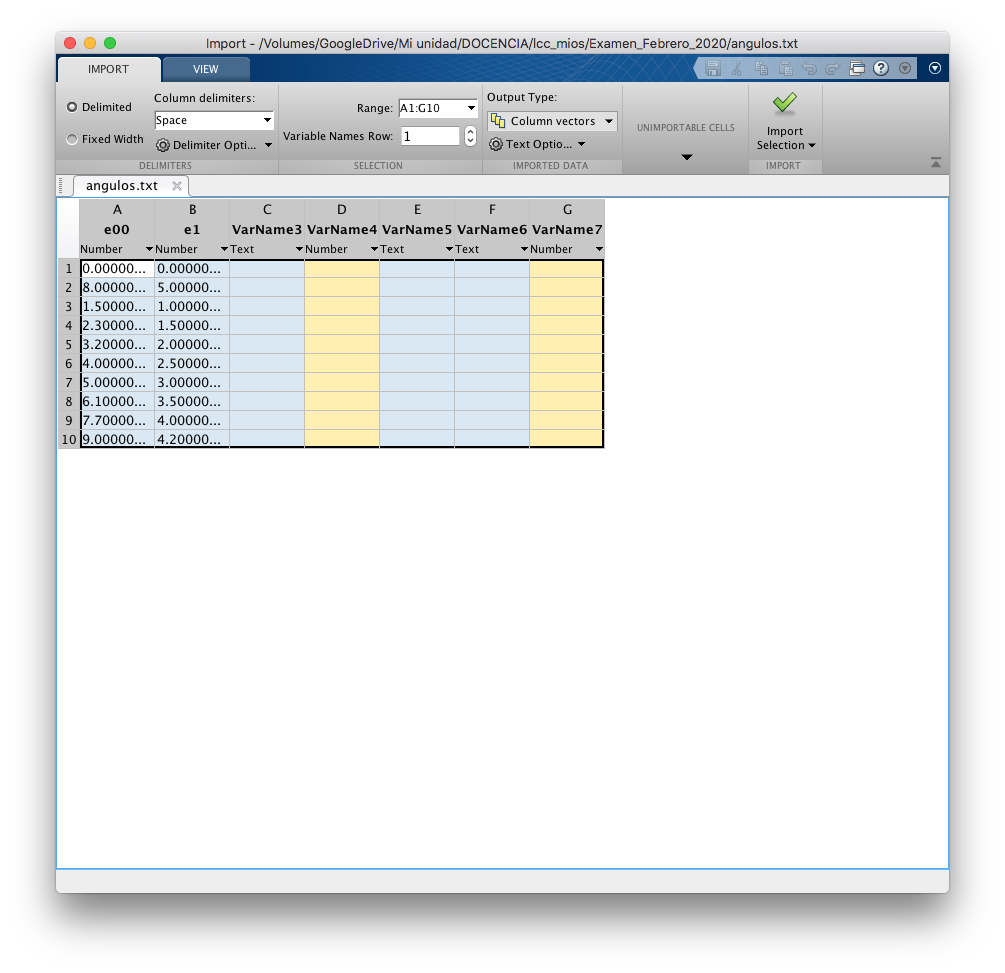
\includegraphics[width=10cm]{Wizard1.png}
	\caption{Aspecto de la herramienta de importaci�n de datos}
	\label{fig:wizard}
\end{figure}

Para abrir en Matlab la herramienta de importaci�n, basta pulsar en la pesta�a \emph{home}, situada en la parte superior del IDE de Matlab,   el bot�n \emph{Import Data}. Matlab abre entonces una ventana que nos permite navegar por el �rbol de directorio y seleccionar el archivo del que deseamos importar los datos. Una vez seleccionado, Matlab abre la ventana mostrada en la imagen \ref{fig:wizard}. 
Se trata de un programa especial ---\emph{import wizard}--- que sirve para guiar al usuario en el proceso de cargar las variables contenidas en el fichero en el \emph{workspace} de Matlab.

\section{Operaciones aritm�ticas, relacionales y l�gicas}\index{Operaciones}

\subsection{Operaciones aritm�ticas}\index{Operaciones!Aritm�ticas}
 Una vez que sabemos como crear o importar variables en Matlab, vamos a ver como podemos realizar operaciones aritm�ticas elementales con ellas. La sintaxis es muy sencilla, y podemos sintetizarla de la siguiente manera:
\begin{equation*}
resultado=operando_1 operador_1 operando_2 operador_2 operando_3 \cdots operando_{n-1} operador_n
\end{equation*}
Es decir basta concatenar los operadores con los operandos y definir una variable en la que guardar el resultado. Por ejemplo,
\begin{verbatim}
>>x=1; y=2; z=3; q=x+y+z
>>z=6
\end{verbatim}
En este caso los operandos son las variables \texttt{x}, \texttt{y}, \texttt{z}, el operador, que se repite dos veces es el s�mbolo \texttt{+} que representa la operaci�n suma y \texttt{q} es la variable en la que se guarda el resultado, en este caso, de la suma de las tres variables anteriores.

Los operadores aritm�ticos disponibles en Matlab cubren las operaciones aritm�ticas habituales, pero hay que recordar que Matlab considera sus variables como matrices. Por lo tanto, las operaciones definidas Matlab las considera por de defecto operaciones entre matrices. La tabla \ref{tabop} contiene los operadores definidos en  Matlab.

\begin{table}[h]
\caption{Operadores aritm�ticos definidos en Matlab}
\label{tabop}
\centering
\begin{tabular}{cccc}
operaci�n&s�mbolo&ejemplo&notas\\
\hline
suma&\texttt{+}&\texttt{r=a+b}&suma matricial\\
\hline
diferencia&\texttt{-}\\
\hline
producto&\texttt{*}&\texttt{r=a*b}&producto matricial\\
producto&\texttt{.*}&\texttt{r=a.*b}&producto por elementos\\
\hline
divisi�n&\texttt{/}&\texttt{d=a/b}& divisi�n: $a\cdot b^{-1}$\\
divisi�n& \texttt{./}& \texttt{d=a./b}& divisi�n por elementos\\
divisi�n& \texttt{\textbackslash}& \texttt{d=a\textbackslash b}& divisi�n por la izquierda: $a^{-1}\cdot b$\\
\hline
potenciaci�n&\texttt{\^}&\texttt{y=a \^\ b}&potencia de una matriz \\
potenciaci�n&\texttt{.\^}&\texttt{y=a .\^\ b}&potencia elemento a elemento\\
\hline
trasposici�n&\texttt{'}&\texttt{y=a'}&matriz traspuesta\\
\hline
\hline
\end{tabular}
\end{table}

A continuaci�n, veremos algunos ejemplos de manejo de operaciones b�sicas. Hemos visto ya el manejo de la suma. Si se trata de matrices en vez de n�meros,

\begin{verbatim}
>> A=[1 2 3; 4 5 6; 7 8 9]

A =

     1     2     3
     4     5     6
     7     8     9

>> B=[4 5 6; 2 0 3; -1 2 4]

B =

     4     5     6
     2     0     3
    -1     2     4

>> C=A+B

C =

     5     7     9
     6     5     9
     6    10    13
\end{verbatim}
 Por supuesto, hay que respetar las condiciones en que es posible realizar una operaci�n aritm�tica entre matrices. La operaci�n,
 
\begin{verbatim}
>> A=[1 2 3; 4 5 6; 7 8 9]

A =

     1     2     3
     4     5     6
     7     8     9

>> B=[4 5 6; 2 0 3]

B =

     4     5     6
     2     0     3

>> C=A+B
Error using  + 
Matrix dimensions must agree.
\end{verbatim}
da un error porque solo es posible sumar matrices del mismo tama�o.\footnote{Ver las definiciones de las operaciones matriciales en el capitulo \ref{opmatr}.}

En el caso del producto, Matlab define dos operaciones distintas. La primera es el producto matricial normal, 
\begin{verbatim}
>> A=[1 2 3; 4 5 6; 7 8 9]
A =

     1     2     3
     4     5     6
     7     8     9

>> B=[3 4; -2 1; 6 7]
B =

     3     4
    -2     1
     6     7

>> P=A*B
P =

    17    27
    38    63
    59    99
\end{verbatim}

El segundo producto, no es propiamente una operaci�n aritm�tica definida sobre matrices. Se trata de un producto realizado elemento a elemento. Para ello los dos factores deben ser matrices del mismo tama�o. El resultado es una nueva matriz de igual tama�o que las iniciales en la que cada elemento es el producto de los elementos que ocupaban la misma posici�n en las matrices factores,

\begin{verbatim}
>> A = [1 2 3; 4 5 6]

A =

     1     2     3
     4     5     6

>> B = [2 3 4; 1 2 3]

B =

     2     3     4
     1     2     3

>> C =A.*B

C =

     2     6    12
     4    10    18
\end{verbatim}

En general, cualquier operador al que se antepone un punto \texttt{.* ./ .\^} indica una operaci�n realizada elemento a elemento.

La divisi�n no est� definida para matrices. Sin embargo, en Matlab hay definidas tres divisiones. La primera, emplea el s�mbolo cl�sico de divisi�n, para simples n�meros realiza la divisi�n normal. Para matrices, la operaci�n es equivalente a multiplicar el primer operando por la matriz inversa del segundo. $A/B \equiv A\cdot B^{-1}$. Las siguientes tres operaciones son equivalentes en Matlab, aunque desde el punto de vista del  c�lculo empleado para obtener el resultado, son num�ricamente distintas,

\begin{verbatim}
>> A=[1 2 3; 4 5 6; 7 8 9]
A =

     1     2     3
     4     5     6
     7     8     9

>> B=[2 0 1; 3 2 -1; -2 0 2]
B =

     2     0     1
     3     2    -1
    -2     0     2

>> C=A/B
C =

    0.6667    1.0000    1.6667
    1.6667    2.5000    3.4167
    2.6667    4.0000    5.1667

>> C=A*inv(B)
C =

    0.6667    1.0000    1.6667
    1.6667    2.5000    3.4167
    2.6667    4.0000    5.1667

>> C=A*B^-1
C =

    0.6667    1.0000    1.6667
    1.6667    2.5000    3.4167
    2.6667    4.0000    5.1667
\end{verbatim}  

En el primer caso se ha empleado la divisi�n, en el segundo se a multiplicado la matriz \texttt{A} por la inversa de \texttt{B}, calcul�ndola mediante la funci�n de Matlab \texttt{inv}, y en el tercer caso se ha multiplicado la matriz \texttt{A} por \texttt{B} elevado a $-1$.

La divisi�n elemento a elemento, funciona de modo an�logo a como lo hace la multiplicaci�n elemento a elemento. 

La divisi�n por la izquierda, representada mediante el s�mbolo \texttt{\textbackslash} es equivalente a multiplicar la inversa del primer operando por el segundo,  $A \backslash B \equiv A^{-1} \cdot B$.
\begin{verbatim}

>> A=[1 2 3; 4 5 6; 3 -4 9]
A =

     1     2     3
     4     5     6
     3    -4     9

>> B=[2 0 1; 3 2 -1; -2 0 2]
B =

     2     0     1
     3     2    -1
    -2     0     2

>> C=A\B
C =

   -0.9000    1.0000   -1.5500
    0.8000         0    0.1000
    0.4333   -0.3333    0.7833

>> C=A^-1*B
C =

   -0.9000    1.0000   -1.5500
    0.8000    0.0000    0.1000
    0.4333   -0.3333    0.7833

>> C=inv(A)*B
C =

   -0.9000    1.0000   -1.5500
    0.8000    0.0000    0.1000
    0.4333   -0.3333    0.7833
\end{verbatim}

Uno de los usos t�picos de la divisi�n por la izquierda, es la resoluci�n de sistema de ecuaciones lineales (ver tema \ref{sistemas}). Por ejemplo, dado el sistema de ecuaciones,

\begin{equation*}
\left. \begin{aligned}
3&x_1+2x_2-4x_3=3\\
2&x_1+ \ \ x_2+3x_3=-3\\
&x_1+3x_2+2x_3=7
\end{aligned}\right\} \Rightarrow	\overbrace{\begin{pmatrix}
3& 2& -4\\
2& 1& \ 3\\
1& 3& \ 2
\end{pmatrix}}^A \cdot \overbrace{\begin{pmatrix}
x_1\\
x_2\\
x_3
\end{pmatrix}}^x=\overbrace{\begin{pmatrix}
 \ 3\\
-3\\
-7
\end{pmatrix}}^b
\end{equation*}

Podemos resolverlo en Matlab con una sencilla divisi�n por la izquierda,

\begin{verbatim}
>> A=[3 2 -4; 2 1 3; 1 3 2]

A =

     3     2    -4
     2     1     3
     1     3     2

>> b=[3;-3;-7]
b =

     3
    -3
    -7

>> x=A\b
x =

     1
    -2
    -1
\end{verbatim}
Aunque la potenciaci�n en Matlab tiene m�s usos, solo consideraremos el caso de una matriz elevada a un n�mero. El resultado ser� multiplicar la matriz por si misma tantas veces como indique el exponente, $A^3=A\cdot A \cdot A$,
\begin{verbatim}
>> A=[3 0 -1; 2 1 0; 1 3 2]

A =

     3     0    -1
     2     1     0
     1     3     2

>> A^3

ans =

    13   -18   -18
    24    -5   -12
    54    18    -5

>> A*A*A

ans =

    13   -18   -18
    24    -5   -12
    54    18    -5

\end{verbatim}

La potenciaci�n elemento a elemento eleva cada elemento de la matriz al valor que indique el exponente,

\begin{verbatim}
>> B = [1 2 3;3 4 5]

B =

     1     2     3
     3     4     5

>> B.^2

ans =

     1     4     9
     9    16    25

\end{verbatim}
Trasponer una matriz es obtener una nueva matriz intercambiando las filas con las columnas de la matriz original, (ver cap�tulo \ref{opmatr}). As� por ejemplo,
\begin{verbatim}
>> A=[3 0 -1 0; 2 1 0 0]

A =
     3     0    -1     0
     2     1     0     0

>> B=A'
B =

     3     2
     0     1
    -1     0
     0     0
\end{verbatim}
Las matrices \texttt{A} y \texttt{B} son traspuestas entre s�.

\subsection{Precedencia de los operadores aritm�ticos}\index{Operadores!Precedencia}
Combinando operadores aritm�ticos, es posible elaborar expresiones complejas. Por ejemplo,
\begin{verbatim}
R=5*3-6/3+2^3+2-4
\end{verbatim}
La pregunta que surge inmediatamente es en qu� orden realiza Matlab las operaciones indicadas. Para evitar ambig�edades, Matlab ---como todos los lenguajes de programaci�n--- establece un orden de precedencia, que permite saber exactamente en qu� orden se realizan las operaciones. En Matlab el orden de precedencia es:
\begin{enumerate}
\item En primer lugar se calculan las potencias.
\item A continuaci�n los productos y las divisiones, que tienen el mismo grado de precedencia.
\item Por �ltimo, se realizan las sumas y las restas. 
\end{enumerate} 

Por tanto, en el ejemplo que acabamos de mostrar, Matlab calcular�a primero,
\begin{verbatim}
2^3=8
\end{verbatim}
a continuaci�n el producto y la divisi�n
\begin{verbatim}
5*3=15
6/3=2
\end{verbatim}
Por �ltimo sumar�a todos los resultados intermedios, y guardar�a el resultado en la variable \texttt{R}
\begin{verbatim}
15-2+8+2-4=19
R=19
\end{verbatim}

\paragraph{Uso de par�ntesis para alterar el orden de precedencia.}
Cuando necesitamos escribir una expresi�n complicada, en muchos casos el necesario alterar el orden de precedencia. Para hacerlo, se emplean par�ntesis. Sus reglas de uso son b�sicamente dos:
\begin{itemize}
\item La expresiones entre par�ntesis tienen precedencia sobre cualquier otra operaci�n.
\item Cuando se emplean par�ntesis anidados (unos dentro de otros) los resultados siempre se calculan del par�ntesis m�s interno hacia fuera.
\end{itemize}

Por ejemplo,
\begin{verbatim}
>> y=2+4/2
y =

     4

>> y=(2+4)/2

y =

     3
\end{verbatim}

En la primera operaci�n, el orden de precedencia de los operadores hace que Matlab divida primero $4$ entre $2$ y a continuaci�n le sume $2$. En el segundo caso, el par�ntesis tiene precedencia; Matlab suma primero $2$ y $4$ y a continuaci�n divide el resultado entre $2$.

El uso correcto de los par�ntesis para alterar la precedencia de los operadores, permite expresar cualquier operaci�n matem�tica que deseemos. Por ejemplo calcular la hipotenusa de un tri�ngulo rect�ngulo a partir de valor de sus catetos,
\begin{equation*}
h=(c_1^2+c_2^2)^{\frac{1}{2}}
\end{equation*}
Que en Matlab podr�a expresarse como,
\begin{verbatim}
h=(c1^2+c2^2)^(1/2)
\end{verbatim}

O la expresi�n general para obtener las ra�ces de una ecuaci�n de segundo grado,

\begin{equation*}
x= \frac{-b\pm(b^2-4\cdot a \cdot c)^{\frac{1}{2}}}{2\cdot a}
\end{equation*}

en este caso es preciso dividir el c�lculo en dos expresiones, una para la ra�z positiva,

\begin{verbatim}
x=(-b+(b^2-4*a*c)^(1/2))/(2*a)
\end{verbatim}
y otra para la ra�z negativa

\begin{verbatim}
x=(-b-(b^2-4*a*c)^(1/2))/(2*a)
\end{verbatim}

Es necesario ser cuidadosos a la hora de construir expresiones que incluyen un cierto n�mero de operaciones. As�, en el ejemplo que acabamos de ver, el par�ntesis final \texttt{2*a} es necesario; si se omite, Matlab multiplicar� por \texttt{a} el resultado de todo lo anterior, en lugar de dividirlo.

\subsection{Operaciones Relacionales y l�gicas.}\index{Operadores! Relaciones y l�gicos}
Aunque son distintas, las operaciones relacionales y las l�gicas estas estrechamente relacionadas entre s�. Al igual que en el caso de las operaciones aritm�ticas, en las operaciones relacionales y l�gicas existen operandos --variables sobre las que se efect�a la operaci�n-- y operadores, que indican cu�l es la operaci�n que se efect�a sobre los operandos. La diferencia fundamental es que tanto en el caso de las operaciones relacionales como l�gicas el resultado solo puede ser $1$ (cierto) o $0$ (falso). 

\paragraph{Operadores relacionales.}La tabla \ref{tabrel} muestra los operadores relacionales disponibles en el entorno de Matlab. Su resultado es siempre la verdad o falsedad de la relaci�n indicada. 

\begin{table}[h]
\caption{Operadores relacionales definidos en Matlab}
\label{tabrel}
\centering
\begin{tabular}{cccc}
\hline
\hline
operaci�n&s�mbolo&ejemplo&notas\\
\hline
menor que &\texttt{<}&\texttt{r=a<b}&Compara matrices elemento a elemento o un \\ 
&&& escalar con todos los elementos de una matriz\\
\hline
mayor que&\texttt{>}&\texttt{r=a>b}& Compara matrices elemento a elemento o un\\ 
&&& escalar con todos los elementos de una matriz\\
\hline
mayor o igual que&\texttt{>=}&\texttt{r=a>=b}&Compara matrices elemento a elemento o un\\ 
&&& escalar con todos los elementos de una matriz\\
\hline
menor o igual que&\texttt{<=}&\texttt{r=a<=b}&Compara matrices elemento a elemento o un\\ 
&&& escalar con todos los elementos de una matriz\\
\hline
igual a&\texttt{==}&\texttt{a==b}&Compara matrices elemento a elemento o un\\ 
&&& escalar con todos los elementos de una matriz\\
\hline
Distinto de& \texttt{a\texttildelow =b}& \texttt{a\texttildelow =b}&Compara matrices elemento a elemento o un\\ 
&&& escalar con todos los elementos de una matriz\\
\hline
\hline
Especificadores\\
\hline 
todos& \texttt{all}& \texttt{r=all(a)}& Verdadero si todos los elementos de un vector\\
&&& son verdaderos. Para matrices el resultado \\
&&& se obtiene para cada columna\\ 
\hline
alguno&\texttt{any}&\texttt{r=any(a)}& Verdadero si alg�n(os) elemento(s) de un vector \\
&&&  son verdadero(s). Para matrices el resultado\\
&&&  se obtiene para cada columna\\
\hline
encontrar&\texttt{find}&\texttt{r=find(a)}&Devuelve como resultado los �ndices\\
&&& de los elementos verdaderos\\
\hline
\hline
\end{tabular}
\end{table} 

Los operadores relacionales pueden trabajar sobre matrices de igual tama�o, en ese caso la operaci�n se realiza elemento a elemento y el resultado es una matriz de unos y ceros. Por ejemplo:
\begin{verbatim}
>> A=[3 0 -1; 2 1 0; 1 3 2]
A =

     3     0    -1
     2     1     0
     1     3     2

>> B=[2 0 1; 3 2 -1; -2 0 2]

B =

     2     0     1
     3     2    -1
    -2     0     2
>> C=A>B

C =

     1     0     0
     0     0     1
     1     1     0
\end{verbatim}

La matriz \texttt{C} contiene el resultado l�gico de comprobar uno a uno si los elementos de \texttt{A} son mayores que los elementos de \texttt{B}; como el elemento \texttt{A(1,1)} es mayor que \texttt{B(1,1)}, la relaci�n es cierta. Por tanto, el resultado \texttt{C(1,1)} es uno. La relaci�n, --en este caso ser mayor que-- se va comprobando elemento a elemento y su verdad o falsedad se consigna en el elemento correspondiente de la matriz resultado.

Por supuesto, si se comparan dos valores escalares el resultado es un tambi�n un escalar,
\begin{verbatim}
>> r=3<=7
r =

     1
\end{verbatim}

Los operadores relacionales admiten tambi�n que uno de sus operandos sea un escalar y el otro una matriz. En este caso, Matlab compara el escalar con todos los elementos de la matriz y guarda el resultado en una matriz del mismo tama�o,
\begin{verbatim}
>> A

A =

     3     0    -1
     2     1     0
     1     3     2

>> menor_que_tres=A<3

menor_que_tres =

     0     1     1
     1     1     1
     1     0     1

>> distinto_de_tres=A~=3

distinto_de_tres =

     0     1     1
     1     1     1
     1     0     1

>> igual_a_tres=A==3

igual_a_tres =

     1     0     0
     0     0     0
     0     1     0
\end{verbatim} 

Es importante se�alar que el operador relacional que permite comparar si dos variables son iguales es \texttt{==} (doble igual), no confundirlo con el igual simple \texttt{=} empleado como sabemos como s�mbolo de asignaci�n.
En cuanto a la tilde,\texttildelow , empleada en el operador \texttt{\texttildelow=}, se obtiene en Matlab pulsando la tecla \texttt{4} mientras se mantiene pulsada la tecla \texttt{alt gr}. la tilde en Matlab representa la negaci�n l�gica. As� por ejemplo si escribimos en Matlab,
\begin{verbatim}
>> ~1
ans =
     0
     
>> ~0
ans =
     1
\end{verbatim}
Si negamos el uno (verdadero) nos da cero (falso) y viceversa.

Hablaremos por �ltimo de los especificadores, incluidos en la parte inferior de la tabla \ref{tabrel}. No son operadores. Se trata de funciones definidas en Matlab.

La funci�n \texttt{any} toma como variable de entrada una matriz. Como veremos en la secci�n siguiente, esto se indica colocando el nombre de la variable de entrada, a continuaci�n del nombre de la funci�n entre par�ntesis. La salida de la funci�n, entendiendo por tal el valor devuelto por la misma, se puede guardar en una variable mediante el s�mbolo de asignaci�n,

\begin{verbatim}
salida=any(entrada)
\end{verbatim}

Si introducimos como entrada un vector fila o un vector columna, la funci�n \texttt{any}, devolver� un uno a la salida, si al menos uno de los elementos del vector de entrada es distinto de cero y devolver� un cero si todos los elementos del vector de entrada son ceros 
\begin{verbatim}
>> s=[1 -2 0 2]
s =

     1    -2     0     2

>> r=any(s)

r =

     1
>> s=zeros(3,1)

s =

     0
     0
     0

>> r=any(s)

r =

     0
\end{verbatim}

Si introducimos como variable de entrada una matriz, la funci�n \texttt{any} buscar� si hay alg�n valor distinto de cero por columnas de la matriz de entrada. 
La salida de la funci�n \texttt{any} ser� entonces un vector fila con el mismo n�mero de columnas que la matriz de entrada. Cada elemento del vector salida toma valor uno,  si la columna correspondiente de la matriz de entrada tiene al menos un valor distinto de cero y toma valor cero si todos los elementos de dicha columna son cero. Por ejemplo, Si definimos en Matlab una matriz,
\begin{verbatim}
>> A=[3 0 -1 0; 2 1 0 0; 1 3 0 0]
A =

     3     0    -1     0
     2     1     0     0
     1     3     0     0


\end{verbatim}  

y le aplicamos la funci�n \texttt{any},

\begin{verbatim}
>> r=any(A)
r =

     1     1     1     0

\end{verbatim}

El primer elemento del vector resultante es $1$, puesto que todos los elementos de la primera columna de $A$ son cero. El segundo tambi�n es uno, porque al menos dos de los elementos de la segunda columna de $A$ son distintos de cero, lo mismo sucede con la tercera que tiene un elemento distinto de cero. Solo el �ltimo elemento de la respuesta es cero ya que todos los elementos de la �ltima columna de $A$ son cero.

La funci�n \texttt{all} funciona de modo an�logo a \texttt{any}, pero en este caso, el vector resultante toma valor uno si todos los elementos de la columna correspondiente de la matriz de entrada son distintos de cero. Si aplicamos \texttt{all} a la misma matriz del ejemplo anterior,

\begin{verbatim}
>> r=all(A)
r =

     1     0     0     0
\end{verbatim} 

Solo el primer elemento del vector salida \texttt{r} es ahora distinto de cero, ya que la matriz \texttt{A} tiene ceros en todas sus columnas menos en la primera.

Queda por se�alar que ambas funciones pueden operar por filas en lugar de hacerlo por columnas. De hecho la funci�n admite un segundo par�metro de entrada que se introduce detr�s de la matriz de entrada y separado por una coma, si dicho par�metro vale $1$ (o se omite, como hemos hecho en los ejemplos anteriores), la funci�n operan por columnas. Si a dicho par�metro se le da valor \texttt{2}, la funci�n opera por filas,
\begin{verbatim}
>> r=any(A,2)
r =

     1
     1
     1

>> r=all(A,2)
r =

     0
     0
     0

\end{verbatim}
En este caso las funciones nos devuelven vectores columnas que indican si en la fila correspondiente de la matriz de entrada hay alg�n elemento distinto de cero (caso del funci�n \texttt{any}) o si todos los elementos son distintos de cero (caso de la funci�n \texttt{all}).

La utilidad de estas dos funciones que acabamos de describir se ve m�s clara cuando las combinamos con el uso de los operadores relacionales.  por ejemplo,
\begin{verbatim}
>> A=[3 0 -1 0; 2 1 0 0; 1 3 0 0]

A =

     3     0    -1     0
     2     1     0     0
     1     3     0     0

>> C=A>2

C =

     1     0     0     0
     0     0     0     0
     0     1     0     0

>> r1=any(C)

r1 =

     1     1     0     0

>> r=any(r1)

r =

     1

\end{verbatim}

 Mediante el uso del operador \texttt{>} y de la funci�n \texttt{any}, hemos comprobado que en la matriz \texttt{A} hay al menos alg�n elemento distinto de cero. Por supuesto, esto podemos hacerlo en una sola sentencia, combinado operadores y funciones,
 
\begin{verbatim}
>> A=[3 0 -1 0; 2 1 0 0; 1 3 0 0]

A =
     3     0    -1     0
     2     1     0     0
     1     3     0     0

>> r=any(any(A>2))

r =
     1
\end{verbatim}

Como un segundo ejemplo, vamos a comprobar si todos los elementos de la matriz \texttt{A} son menores que 4,
\begin{verbatim}
>> A=[3 0 -1 0; 2 1 0 0; 1 3 0 0]
A =

     3     0    -1     0
     2     1     0     0
     1     3     0     0

>> r=all(all(A<4))

r =

     1
\end{verbatim}

Por �ltimo, insistir en que, si no se indica otra cosa,\texttt{any} and \texttt{all}, trabajan buscando los valores distintos de cero por columnas. As� por ejemplo la sentencia,
\begin{verbatim}
>> r=any(all(A>2))
r =

     0
\end{verbatim}
comprueba si en \emph{alguna} de las columnas de \texttt{A} \emph{todos} los elementos son menores que $2$. y la sentencia,
\begin{verbatim}
>> r=all(any(A>-1))
r =

     1
\end{verbatim}
comprueba si en \emph{todas} las columnas de \texttt{A} hay \emph{alg�n} elemento mayor que $-1$.

La �ltima de las funciones incluidas en la tabla \ref{tabrel} es la funci�n \texttt{find}. Esta funci�n admite como variable de entrada una matriz. Si se la llama con una sola variable de salida, devuelve un vector con los �ndices de los elementos de la matriz que son distintos de cero. Si se la llama con dos variables de salida en la primera devuelve un vector con el �ndice de las filas de los elementos de la matriz distintos de cero, y en la segunda variable devuelve un vector con los �ndices de las correspondientes columnas de los elementos de la matriz distintos de cero,

\begin{verbatim}
>> A

A =

     1     0     1
     0     1     1
     1     1     0

>> indice=find(A)
indice =

     1
     3
     5
     6
     7
     8
\end{verbatim}

Los elementos 1, 3 ,5, 6, etc, de la matriz $A$ son distintos de cero (ver indexaci�n con un �nico �ndice \ref{index})

\begin{verbatim}
>> [fila,columna]=find(A)

fila =

     1
     3
     2
     3
     1
     2


columna =

     1
     1
     2
     2
     3
     3

>> 
\end{verbatim}

Los elementos (1,1), (3,1), (2,2), etc, de la matriz $A$ son distintos de cero.

Podemos combinarlos con otros operadores relacionales para conocer qu� elementos de una matriz cumplen una determinada condici�n. Por ejemplo:

\begin{verbatim}
>> A=[3 0 -1 0; 2 1 0 0; 1 3 0 0]
A =

     3     0    -1     0
     2     1     0     0
     1     3     0     0
     
>> indice=find(A~=0)

indice =

     1
     2
     3
     5
     6
     7
\end{verbatim}

Nos permite conocer los �ndices de los elementos de $A$ que son distintos de cero. Como hemos dado una solo variable de salida, Matlab emplea un �nico �ndice para darnos la posici�n de los elementos distintos de cero (ver la secci�n indexaci�n, pag. 37) para obtener los dos �ndices de cada elemento distinto de cero de la matriz \texttt{A} del ejemplo anterior basta llamar a la funci�n con dos variables de salida,

\begin{verbatim}
>> [fila, columna] = find(A~=0)

fila =

     1
     2
     3
     2
     3
     1

columna =

     1
     1
     1
     2
     2
     3
\end{verbatim} 

\paragraph{Operadores L�gicos}
En Matlab se distinguen tres conjuntos de operadores l�gicos seg�n el tipo de variable sobre la que act�en. Aqu� vamos a ver solo dos de ellos: los operadores l�gicos elemento a elemento y los operadores l�gicos para escalares.

La tabla \ref{tablo1} muestra los operadores l�gicos elemento a elemento. Estos operadores l�gicos esperan que sus operando sean matrices de igual tama�o, aunque pueden actuar tambi�n sobre escalares. 

El resultado, es una matriz del mismo tama�o que los operandos, compuesta por ceros y unos, que son el resultado de la operaci�n l�gica realizada entre los elementos de los operandos que ocupan la misma posici�n en sus respectivas matrices.

\begin{table}[h]
\caption{Operadores l�gicos elemento a elemento}
\label{tablo1}
\centering
\begin{tabular}{cccc}
\hline
\hline
operaci�n&s�mbolo&ejemplo&notas\\
\hline
and&\texttt{\&}&\texttt{r=a\&b}&Operaci�n l�gica \emph{and} entre los elementos de \texttt{a} y \texttt{b} \\ 
\hline
or &\texttt{\textbar}&\texttt{r=a\textbar b}& Operaci�n l�gica \emph{or} entre los elementos de \texttt{a} y \texttt{b}\\
\hline
or exclusivo&\texttt{xor()}&\texttt{r=xor(a,b)}&Operaci�n l�gica \emph{or exclusivo} \\
&&& entre los elementos de \texttt{a} y \texttt{b}\\
\hline
negaci�n&\texttt{\texttildelow}&\texttt{r=\texttildelow a}&complemento de los elementos de \texttt{a}\\ 
\hline
\hline
\end{tabular}
\end{table} 

En cuanto a su funcionamiento, son los operadores t�picos del �lgebra de Bool. As� el operador \texttt{\&} sigue la tabla de verdad propia de la operaci�n \emph{and}, el resultado solo es verdadero ($1$) si sus operandos son verdaderos ($1$)\footnote{En realidad Matlab considerar� verdadero cualquier operando distinto de $0$},

\begin{table}[h]
\begin{tabular}{c|c|c}
\multicolumn{3}{c}{Tabla de verdad de la operaci�n \texttt{and}}\\
\hline
\hline
operando 1&operando 2 &Resultado\\ 
\hline
1&1&1\\
1&0&0\\
0&1&0\\
0&0&0\\ 
\hline
\hline
\end{tabular}
\end{table} 

As� por ejemplo,

\begin{verbatim}
>> A=[1 0 1; 0 1 1;1 1 0]
A =

     1     0     1
     0     1     1
     1     1     0

>> B=[1 1 1; 0 0 1; 1 0 1]
B =

     1     1     1
     0     0     1
     1     0     1

>> R=A&B
R =

     1     0     1
     0     0     1
     1     0     0
\end{verbatim}

La matriz \texttt{R} contiene el resultado de realizar la operaci�n \texttt{and} elemento a elemento entre las matrices \texttt{A} y \texttt{B}; solo aquellas posiciones que contienen a la vez un $1$ en ambas matrices, obtienen un $1$ como resulta en la matriz \texttt{R}.

La operaci�n \texttt{or}, responde a la siguiente tabla de verdad,

\begin{table}[h]
\begin{tabular}{c|c|c}
\multicolumn{3}{c}{Tabla de verdad de la operaci�n \texttt{or}}\\
\hline
\hline
operando 1&operando 2 &Resultado\\ 
\hline
1&1&1\\
1&0&1\\
0&1&1\\
0&0&0\\ 
\hline
\hline
\end{tabular}
\end{table} 

En  este caso, el resultado es cierto si cualquiera de los dos operando es cierto. Si lo aplicamos a las matrices del ejemplo anterior,

\begin{verbatim}
>> r=A|B
r =

     1     1     1
     0     1     1
     1     1     1
\end{verbatim}

Solo es cero el elemento \texttt{r(2,1)} de la matriz resultado, ya que solo los elementos \texttt{A(2,1)} y \texttt{B(2,1)} son a la vez cero.

La tabla de verdad de la operaci�n \emph{or exclusivo} es,
\begin{table}[h]
\begin{tabular}{c|c|c}
\multicolumn{3}{c}{Tabla de verdad de la operaci�n \texttt{xor}}\\
\hline
\hline
operando 1&operando 2 &Resultado\\ 
\hline
1&1&0\\
1&0&1\\
0&1&1\\
0&0&0\\ 
\hline
\hline
\end{tabular}
\end{table} 
  
Es decir la salida solo es verdadera cuando una de las entradas en verdadera y la otra no. Esta operaci�n solo existe en Matlab con formato de funci�n. Usando de nuevo el ejemplo anterior,

\begin{verbatim}
>> r=xor(A,B)

r =

     0     1     0
     0     1     0
     0     1     1
\end{verbatim}

se puede comprobar que solo son uno los elementos de \texttt{r} para los cuales los correspondientes elementos de \texttt{A} y \texttt{B} no son uno o cero a la vez.

El operador negaci�n act�a sobre un solo operando, neg�ndolo es decir, transformando sus elementos con valor uno en ceros y sus elementos con valor cero en unos.

\begin{verbatim}
>> A
A =

     1     0     1
     0     1     1
     1     1     0

>> r=~A
r =

     0     1     0
     1     0     0
     0     0     1

\end{verbatim}

Para entradas escalares se definen dos operadores l�gicos, que se corresponden con los operadores \emph{and} y \emph{or} de la l�gica de Bool. Por tanto siguen las tablas de verdad de dichas funciones que acabamos de ver. Su sintaxis es la misma que la de los operadores l�gicos elemento a elemento, simplemente se escribe dos veces el s�mbolo del operador para indicar que se trata de una operaci�n entre escalares. As�, por ejemplo para la operaci�n \texttt{and},
\begin{verbatim}
>> a=1
a =

     1

>> b=0
b =

     0


>> r=a&&b
r =

     0
\end{verbatim}
 y para la operaci�n \texttt{or},
 
\begin{verbatim}
>> r=a||b
r =

     1
\end{verbatim}

Los operadores l�gicos elemento a elemento tambi�n funcionan correctamente cuando act�an sobre escalares, pero son, en general menos eficientes que los operadores espec�ficos que acabamos de ver.

Por �ltimo, indicar que los operadores l�gicos pueden combinarse entre s� con operadores relacionales y con operadores aritm�ticos. El orden de precedencia es el siguiente:
\begin{enumerate}
\item  Par�ntesis ()
\item  Operadores aritm�ticos en su orden de precedencia
\item  Operadores relacionales, todos tienen el mismo orden de precedencia por lo que se eval�an de izquierda a derecha
\item \texttt{and} elemento a elemento
\item \texttt{or} elemento a elemento
\item \texttt{and} escalares
\item \texttt{or} escalares
\end{enumerate}

Matlab aconseja el uso de par�ntesis cuando se encadenan varias operaciones l�gicas para asegurar su uso correcto y facilitar la lectura de las sentencias.

Por ejemplo,
\begin{verbatim}
>> A=[3 0 0; 2 1 0; 1 3 0]
A =

     3     0     0
     2     1     0
     1     3     0

>> B=[2 0 1; 3 2 -1; -2 0 2]
B =

     2     0     1
     3     2    -1
    -2     0     2

>> r=A>1&B>A
r =

     0     0     0
     1     0     0
     0     0     0

>> r=(A>1)&(B>A)
r =

     0     0     0
     1     0     0
     0     0     0
\end{verbatim}

Ambas sentencias realizan la misma operaci�n, Comprueban qu� elementos de \texttt{A} son mayores que $1$ y a la vez cumplen ser menores que el correspondiente elemento de \texttt{B}. Sin embargo, los par�ntesis de la segunda sentencia facilitan entender el orden en que se realizan las operaciones. 



\section{Scripts y Funciones} \label{funciones}
Hasta ahora, hemos manejado siempre Matlab desde la l�nea de comandos. Es decir, hemos introducido las instrucciones en Matlab en la ventana de comandos. Este modo de emplear Matlab es poco eficiente, ya que exige volver a introducir todos los comandos de nuevo cada vez que queremos repetir un c�lculo

Matlab puede emplear ficheros de texto en los que introducimos un conjunto de comandos, guardarlos, y volver a emplearlos siempre que queramos. Esta es la forma habitual de trabajar no solo de Matlab, sino de otros muchos entornos de programaci�n. Un fichero que contiene c�digo de Matlab recibe el nombre gen�rico de \emph{programa}. Un programa de Matlab no es m�s que un fichero de texto que contiene l�neas formadas por comando v�lidos de Matlab. Lo habitual es que cada l�nea contenga un comando. El fichero se guarda con un nombre y la extension \texttt{.m}. Por ejemplo: \texttt{miprograma.m}. El nombre del fichero, puede contener n�meros y letras, pero el primer car�cter debe ser siempre una letra. Los programas en Matlab pueden tomar dos formas b�sicas, \emph{scripts} y \emph{funciones}.

\subsection{El editor de textos de Matlab.} \index{Editor de textos}
Podemos emplear un editor de textos cualquiera, que genere texto en ASCII, como por ejemplo el 'block de notas', para escribir nuestros programas. Sin embargo, si trabajamos en el entorno de Matlab, lo ideal es emplear su propio editor de textos. Hay varias formas de abrir el editor de textos de Matlab; la m�s sencilla es pulsar  el icono de nuevo documento (\emph{New Script}) o bien desplegando el men� \emph{New} y seleccionando \emph{script}, la posici�n de ambos se indica en la figura \ref{fig:opened}, dentro de la pesta�a \emph{home} del IDE de matlab.
\begin{figure}[h]
\centering
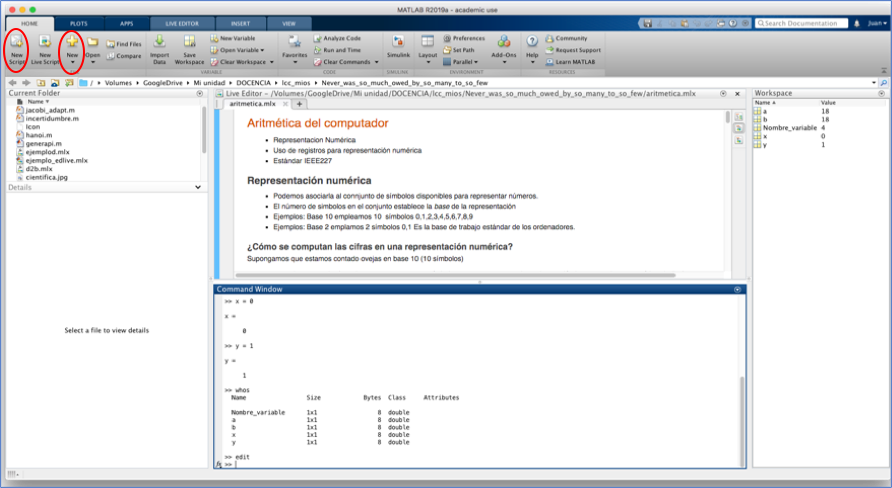
\includegraphics[width=14cm]{opened.png}
\caption{posici�n del bot�n  \emph{New Script} y del  men� \emph{New} en el IDE de Matlab (Se�alados en rojo}.
\label{fig:opened}
\end{figure}

La otra opci�n es emplear el comando \texttt{edit}. Este comando puede emplearse de dos maneras. Si se escribe en la ventana de comandos,

\begin{verbatim}
>>edit
\end{verbatim}
Matlab abrir� el editor de textos y crear� un documento nuevo sin nombre (\emph{untitled}.

Si a�adimos a continuaci�n del comando \texttt{edit} el nombre de un fichero,
\begin{verbatim}
>>edit ejemplo1.m
\end{verbatim}

Buscar� un fichero con dicho nombre en los directorios de Matlab y en el directorio de trabajo. Si lo encuentra, abrir� el archivo encontrado. Si no lo encuentra, crear� uno nuevo con dicho nombre. La figura \ref{fig:edv} muestra el editor de textos de Matlab ---Integrado en la parte central superior del IDE de Matlab--- con el contenido del fichero \texttt{ejemplo1.m}. Adem�s, de entre las pesta�as situadas en la parte superior del IDE, se ha seleccionado la marcada como \emph{EDITOR}. Es posible observar las barras de men� y de herramientas de las que dispone el editor de texto, para facilitar el trabajo de programaci�n. 
\begin{figure}[h]
\centering
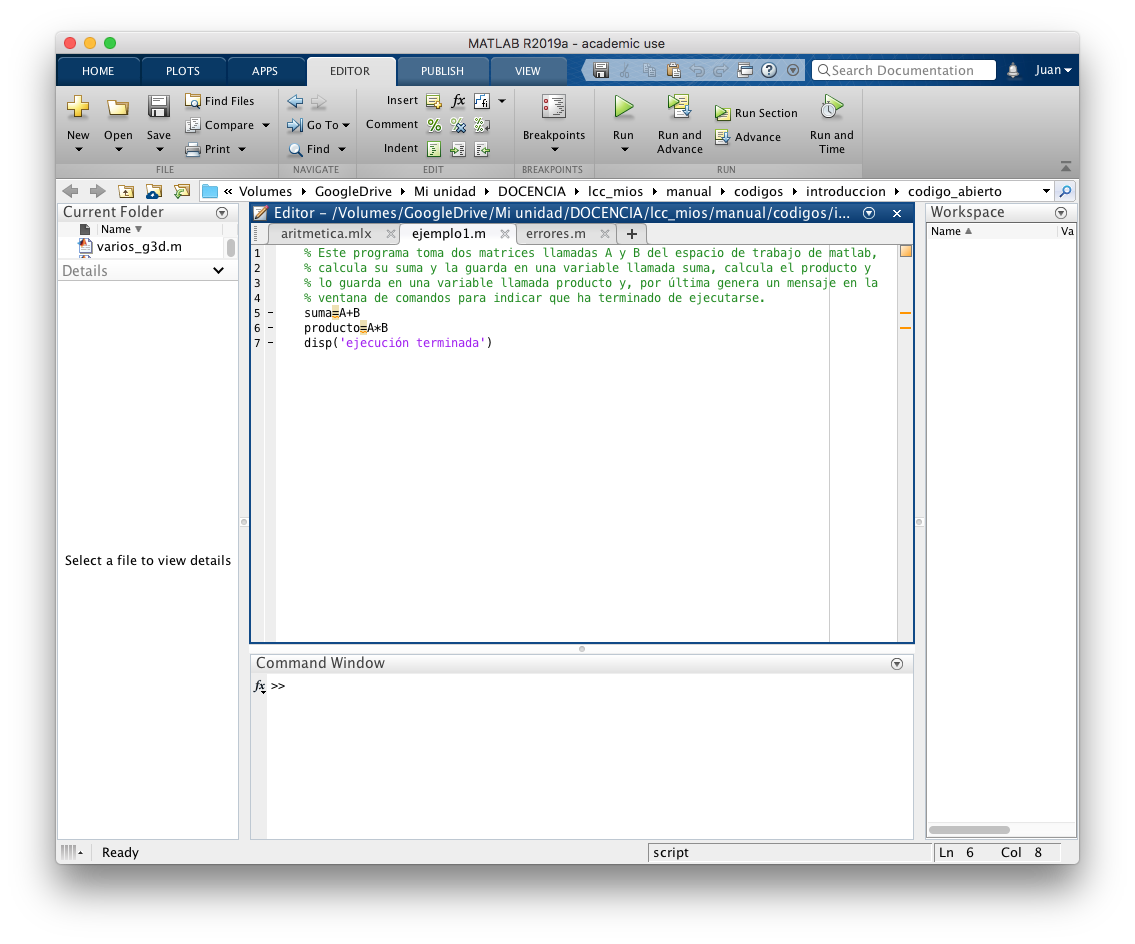
\includegraphics[width=14cm]{ejemplo1.png}
\caption{Vista del editor de textos de Matlab mostrando el contenido del fichero ejemplo1.m}
\label{fig:edv}
\end{figure}
�stas, entre otras facilidades --resaltar texto de palabras clave, cotar n�mero de l�neas, sangrar estructuras de programaci�n, etc.-- hacen que resulte especialmente atractivo emplear el editor de textos de Matlab en lugar de emplear otro editor de textos gen�rico.

\subsection{Scripts} \index{Script}
Un script en Matlab es un simple fichero de texto que contiene un conjunto de sentencias de Matlab v�lidas. La manera de ejecutarlo, consiste en escribir el nombre del fichero en la l�nea de comandos de Matlab. Matlab va leyendo el contenido del fichero l�nea a l�nea, y va ejecutando los comandos que contiene cada l�nea exactamente igual que si se hubieran escrito directamente en la l�nea de comandos de Matlab. Veamos un ejemplo sencillo, que corresponde con el c�digo contenido en la figura \ref{fig:edv}:
\begin{lstlisting}
% Este programa toma dos matrices llamadas A y B del espacio de trabajo de
%  Matlab, calcula su suma y la guarda en una variable llamada suma, calcula el 
% producto y lo guarda en una variable llamada producto y, por �ltima genera un 
% mensaje en la ventana de comandos para indicar que ha terminado de ejecutarse.
suma=A+B
producto=A*B
disp('ejecuci�n terminada') 
\end{lstlisting}
Si escribimos el texto anterior en un archivo y lo guardamos con el nombre ejemplo1.m, podemos ejecutar su contenido en Matlab sin m�s que escribir en la l�nea de comandos:
\begin{verbatim}
>> ejemplo1
\end{verbatim}

Las cuatro primeras l�neas de c�digo que empiezan con el s�mbolo \% no se ejecutan. Cuando Matlab encuentra una l�nea que empieza con dicho s�mbolo interpreta que se trata de un comentario escrito por el programador, para explicar qu� hace el programa o aclarar alg�n aspecto de su funcionamiento. Cuando el editor de Matlab detecta el s�mbolo \% en una l�nea de c�digo, resalta en color verde todo el texto de la l�nea a partir de dicho s�mbolo. De este modo, es inmediato ver que se trata de un comentario y que Matlab no tratar� de ejecutarlo.

Un aspecto importante de la programaci�n en Matlab, y en cualquier otro lenguaje de programaci�n, lo constituye el comentario del c�digo de programa; facilita su uso por otros usuarios y permite al programador recordar qu� fue lo que hizo cuando lo program�. La experiencia demuestra que, en poco tiempo, los programas no comentados se vuelven incompresibles incluso para quien los escribi�.

La quinta l�nea del programa busca en el \emph{workspace} las variables \texttt{A} y \texttt{B}. Si las variables no existen, es decir, si no han sido creadas previamente, el programa da un error, exactamente igual que si hubi�ramos escrito directamente en la ventana de comandos de Matlab la sentencia \texttt{suma=A+B} sin haber definido antes \texttt{A} y \texttt{B}. Si las variables existen calcula la suma y guarda el resultado en el \emph{workspace} en la variable \texttt{suma}. La siguiente l�nea de c�digo realiza el c�lculo del producto de las dos variables y guarda el resultado en la variable \texttt{producto}. La �ltima l�nea del programa mostrar� en la ventana de comandos la frase,

\begin{verbatim}
ejecuci�n terminada
\end{verbatim}
Para ello emplea la funci�n de Matlab \texttt{disp} que escribe en la ventana de comandos cadenas de caracteres.

Un aspecto muy importante de los \emph{scripts} es que hacen uso del \emph{workspace} de Matlab tanto para buscar las variables que emplean como para guardar las variables resultantes de sus c�lculo. Su ejecuci�n es id�ntica a la que se realizar�a si copi�ramos l�nea a l�nea en la ventana de comandos y las fu�ramos ejecutando una detr�s de otra.

\subsection{Funciones} \index{Funciones! Definici�n de funciones en matlab}
Las funciones juegan un papel fundamental en cualquier lenguaje de programaci�n. En el caso de Matlab, se escriben como ficheros de texto, de modo an�logo a los \emph{scripts}. lo que determina que Matlab los interprete como funciones es su primera l�nea de c�digo.  Nos referiremos a esta primera l�nea con el nombre de \emph{cabecera de la funci�n}. La cabecera de una funci�n debe empezar siempre por la palabra clave \texttt{function}. Debe contener adem�s, como m�nimo, el nombre de la funci�n. Por ejemplo,
\begin{verbatim}
function raices
\end{verbatim}

Un detalle importante en Matlab es que el fichero de texto que contiene la funci�n debe llamarse igual que �sta, para que Matlab pueda identificar la funci�n correctamente. Es decir, en el caso del ejemplo anterior, el fichero que contenga la funci�n debe llamarse ra�ces.m.

A parte del nombre de la funci�n la cabecera puede incluir tambi�n nombres de las variables de entrada. Estos se escriben a continuaci�n del nombre de la funci�n, separadas por comas y encerradas entre par�ntesis,

\begin{verbatim}
function raices(a,b,c)
\end{verbatim}

En este ejemplo \texttt{a}, \texttt{b} y \texttt{c} son variables de entrada de la funci�n \texttt{raices}. La raz�n por la que hay que incluir estas variables de entrada es que, a diferencia de los \emph{scripts}, las funciones no pueden acceder directamente a los valores de las variables contenidos en el \emph{workspace} de Matlab. Cuando se ejecuta una funci�n es preciso dar valores a las variables que necesite utilizar, y que no se definan expresamente en el c�digo de la funci�n. Aclararemos esto m�s tarde con un ejemplo.

Por �ltimo la cabecera de una funci�n puede incluir tambi�n una o varias variables de salida. Estas se escriben delante del nombre de la funci�n separadas por comas y encerradas entre corchetes. Entre la(s) variable(s) de salida y el nombre de la funci�n se incluye el s�mbolo de asignaci�n \texttt{=}, para indicar que los resultados obtenidos por la funci�n se han asignado (guardado en) a dichas variables.

\begin{verbatim}
function [x1,x2]=raices(a,b,c)
\end{verbatim}
  
En este caso, las variables de salida ser�an \texttt{x1} y \texttt{x2}.

A continuaci�n, vamos a completar el ejemplo para el que hemos construido la cabecera en los p�rrafos anteriores. Se trata de una funci�n que obtiene las ra�ces de una ecuaci�n de segundo grado, $ax^2+bx+c=0$ conocidos sus coeficientes $a, b, c$,

\lstinputlisting{../codigo/matlab/introduccion/raices.m}

Deberemos guardar estas l�neas de c�digo en un archivo con el nombre raices.m. Podemos ahora emplear la funci�n \texttt(raices) para calcular las ra�ces de una ecuaci�n de segundo grado. Supongamos que queremos obtener las ra�ces de la ecuaci�n,
\begin{equation*}
x^2+x-6
\end{equation*}

si escribimos en la l�nea de comandos,
\begin{verbatim}
>>[raiz1, raiz2]=raices(1,1,-6)
\end{verbatim}
Matlab mostrar� en la pantalla,

\begin{verbatim}
x1 =

     2
     
x2 =

    -3


raiz1 =

     2


raiz2 =

    -3

\end{verbatim}

Analicemos con un poco de detalle lo que hemos hecho. Al escribir: \texttt{[raiz1,raiz2] =} \texttt{raices (1,1,-6)}, hemos \emph{llamado} a la funci�n \texttt{raices}, indicando que las variables de entrada deben tomar los valores \texttt{a=1},\texttt{b=1}, \texttt{c=-6}, es decir, los valores de los coeficientes de la ecuaci�n de segundo grado cuya soluci�n queremos obtener. Adem�s hemos pedido a Matlab que guarde los resultados en el \emph{workspace} en las variable \texttt{raiz1} y \texttt{raiz2}. Cuando, tras llamar a la funci�n, pulsamos el retorno de carro, Matlab empieza a ejecutar el c�digo de la misma. Lo primero que hace es crear las variables \texttt{a}, \texttt{b} y \textbf{c} y asignarle los valores 1,1 y -6. Matlab crea estas variables pero no las guarda en el workspace sino en un espacio de memoria al que solo tiene acceso la funci�n \texttt{raices}, desde la que se han creado. 
Esto constituye una caracter�stica muy importante de las funciones en Matlab. Cada vez que se llama a una funci�n, se crea un espacio de memoria en la que se guardan las variable definidas en la funci�n y a la que solo �sta tiene acceso. Adem�s, una funci�n no puede acceder ni modificar directamente ninguna variable que est� en el \emph{workspace}.

Una vez que la funci�n ha asignado valores a las variable de entrada, comienza a realizar los c�lculos pedidos, en primer lugar calcula la ra�z correspondiente al discriminante positivo,
\begin{equation*}
+\sqrt{b^2-4ac}
\end{equation*}
y crea la variable \texttt{x1} para guardar el resultado. La variable \texttt{x1} solo existe en la memoria de la funci�n \texttt{raices} y por tanto no existe ni es accesible desde el \emph{workspace}. Como no hemos terminado la l�nea de programa en la que se calcula \texttt{x1} con un punto y coma, Matlab muestra en la ventana de comandos el resultado del c�lculo realizado. 

La ra�z correspondiente al discriminante negativo se calcula de modo an�logo. Una vez terminada la ejecuci�n de la l�neas del programa, Matlab vuelve a examinar la cabecera del programa y observa que debe dar como resultado, los valores contenidos en las variables \texttt{x1} y \texttt{x2}. Para ello, crea la variable \texttt{raiz1}  en el \emph{workspace} y copia en ella el contenido de la variable \texttt{x1}. An�logamente crea la variable \texttt{raiz2} y copia en ella el contenido de la variable \texttt{x2}. Con esto ha terminado la ejecuci�n del programa. Matlab destruye las variables \texttt{x1} y \texttt{x2} que solo han existido durante la ejecuci�n del programa, y nos muestra de nuevo el \emph{prompt} en la ventana de comandos para indicarnos que esta listo para ejecutar nuevas �rdenes. Si analizamos el contenido del \emph{workspace}, empleando el comando \texttt{who} de Matlab,
\begin{verbatim}
>> who

Your variables are:

raiz1  raiz2  

\end{verbatim}
observaremos que all� est�n las variable \texttt{raiz1} y \texttt{raiz2}, que contienen las ra�ces de la ecuaci�n de segundo grado que quer�amos resolver.

En el ejemplo anterior hemos asignado directamente valores a las variables de entrada de la funci�n \texttt{raices}. En Matlab, una funci�n puede tambi�n asignar valores a sus variable de entrada copi�ndolos de los de otras variables existentes en el workspace, supongamos que creamos en el workspace de Matlab, tres variables con los valores de los coeficientes de la ecuaci�n de segundo grado del ejemplo anterior,
\begin{verbatim}
>>coef1=1, coef2=1 coef3=-6
\end{verbatim}

Podr�amos entonces llamar a nuestra funci�n ra�ces, sustituyendo los valores de la variables de entrada por los nombres de �stas variables,

\begin{verbatim}
>> [raiz1, raiz2]= raices(coef1,coe2,coef3)
\end{verbatim} 
 Matlab, copiar� ahora los valores contenidos en \texttt{coef1}, \texttt{coef2} y \texttt{coef3} en las variables de entrada de la funci�n \texttt{a}, \texttt{b}, \texttt{c}. Ni que decir tiene, que el resultado final de la ejecuci�n ser� el mismo.

\paragraph{�mbito de una variable} \index{Variable! �mbito de una variable}\index{Variable!�mbito}La importancia del concepto de funci�n est� precisamente en el tratamiento que hace de las variables. Para entenderlo mejor, introduciremos el concepto de \emph{�mbito} de una variable.

Como hemos visto, la forma usual de crear una variable en Matlab es mediante el s�mbolo de asignaci�n. Cuando asignamos un valor o el resultado de una operaci�n a una variable en la ventana de comandos de Matlab,

\begin{verbatim}
>> a=18

a =

    18

\end{verbatim} 
 
Matlab reserva un espacio de memoria del computador para guardar la variable con el valor asignado. Esta variable forma parte del \emph{workspace} de Matlab, que constituye su �mbito propio. La variable creada es solo visible para aquellos comandos y sentencias que,
\begin{enumerate}
\item Se ejecutan desde la ventana de comandos de Matlab.
\item Se ejecutan desde un script.
\end{enumerate}

Cuando ejecutamos una funci�n desde la ventana de comandos de Matlab, la funci�n crea su propio espacio de memoria. Por as� decir, es como un \emph{workspace} particular de la funci�n. Cualquier variable que cree la funci�n se guardar� en el espacio de memoria de la funci�n, que constituir� su �mbito propio. La variable creada dentro de la funci�n solo es visible para aquellos comandos y sentencias que se ejecutan dentro de la funci�n.

Una vez que termina la ejecuci�n de una funci�n, el espacio de memoria que se cre� al ejecutarse se destruye y con �l cualquier variable que el programa haya creado durante su ejecuci�n.

La �nica manera de pasar informaci�n contenida en una variable del \emph{workspace} de Matlab a una funci�n es copi�ndola a una variable de entrada de la funci�n.

La �nica manera de pasar informaci�n contenida en una variable del espacio de memoria de una funci�n, al workspace de Matlab, es copi�ndola a trav�s de una variable de salida de la funci�n.


\begin{figure}[h]
\centering
\begin{tikzpicture}
%\usetikzlibrary{shapes.multipart}
\path (5,0) node(a) [rectangle split,rectangle split parts =2,draw=blue,top color=white,bottom color=blue!15, very thick,align=left,rounded corners]{Ventana de comandos de Matlab
\nodepart{two}
\textgreater \textgreater a=3\\
\textgreater \textgreater b=2\\
\textgreater \textgreater y=ejem(a)\\
y =\\
    12\\
\textgreater \textgreater}		
(0,-7) node(b)[rectangle split,rectangle split parts =2,draw=blue, thick,rounded corners,align=left]{\emph{workspace de Matlab}\\
\nodepart{two}
a=3\\
b=2\\
...\\
tras ejecutar ejem\\
y=12
}
(10,-7) node(c)[rectangle split,rectangle split parts =2,draw=red,thick,rounded corners,align=left]{Espacio de memoria\\ de la funcion\\ \texttt{ejem.m}
\nodepart{two}
ent=3\\
b=4\\
sal=12\\
...\\
tras ejecutar ejem\\
se destruyen\\
todas las variables}
(5,-7) node(d)[rectangle,draw=red,top color=white, bottom color=red!15,align=left,very thick, rounded corners]{function sal=ejem(ent)\\ 
b=4;\\
sal=b*ent;}
(5,-5)node(e)[circle,draw=black,left color=blue!20,right color=red!20,thick,align=center]{Copiar\\ a en ent}
(5,-9)node(f)[circle,draw=black,left color=blue!20,right color=red!20,thick,align=center]{Copiar\\ sal en y};
\draw[blue,-latex](a.west)to [out=180, in=90]node[auto,swap]{Crea a y b} (b);
\draw[blue,-latex](a.south west)to [out=225, in=135]node[auto,align=center]{llamada a la\\ funci�n\\ ejem($\cdot$)} (d.north west);
\draw[black,-latex](b.north east)to [out=45, in=180](e);
\draw[black,-latex](e.east)to [out=0, in=135](c.north west);
\draw[red,-latex](d.north)to [out=90, in=270](e);
\draw[black,-latex](c.south west)to [out=225, in=0](f);
\draw[black,-latex](f.west)to [out=180, in=315](b.south east);
\draw[red,-latex](d.south)to [out=270, in=90](f);
\draw[red,-latex](d.east)to node[auto,swap,align=center]{Crea b\\ y sal}(c);
\draw[red,-latex](d.north east)to [out=45, in=315]node[auto,align=center]{devoluci�n\\ control\\ ventana de comandos} (a.south east);
\end{tikzpicture}
\caption{Ejemplo de uso de memoria y �mbito de variables durante la ejecuci�n de una funci�n}
\label{fig:amb}
\end{figure} 

La figura \ref{fig:amb} muestra esquem�ticamente como se gestionan las variables en Matlab. En el cuadro superior se muestra la ejecuci�n de varias sentencias en la ventana de trabajo de Matlab. Las dos primeras crean directamente dos variables \texttt{a} y \texttt{b} que se almacenan en el \emph{workspace de Matlab}, representado por el cuadro azul de la derecha. 
A continuaci�n se llama a la funci�n ejem (cuadro rojo central), asign�ndole como variable de entrada la variable \texttt{a} y como variable de salida la variable \texttt{y}. La ventana de comandos \emph{cede} el control a la funci�n que empieza a ejecutarse:
\begin{enumerate}
\item La funci�n crea su propio espacio de memoria (cuadro rojo de la izquierda)
\item Copia el valor contenido en la variable \texttt{a} en la variable \texttt{ent}. Esta variable se almacena en el espacio de memoria de la funci�n.
\item Crea la variable \texttt{b} asign�ndole el valor 4 y la guarda en el espacio de memoria de la funci�n. 

A partir de este momento y hasta el final de la ejecuci�n de la funci�n hay dos variables con el mismo nombre: \texttt{b=2} en el \emph{workspace} de Matlab; \texttt{b=4} en el espacio de memoria de la funci�n. Las dos variables coexisten pero no se pueden confundir porque pertenecen a �mbitos distintos.
\item Crea la variable sal asign�ndole el producto de \texttt{b=4} por \texttt{ent=3}. Almacena la variable sal en el espacio de memoria de la funci�n.
\item La funci�n a llegado al final de su c�digo. vuelve a leer la cabecera y crea la variable \texttt{y} en el workspace de Matlab, copiando el contenido de la variable \texttt{sal}.
\item termina la ejecuci�n destruyendo el espacio de memoria de la funci�n y \emph{devolviendo} el control a la ventana de comandos.
\end{enumerate}

\paragraph{Llamar a una funci�n desde otra funci�n.}
En Matlab, como en cualquier lenguaje de alto nivel, es posible llamar una funci�n desde dentro de otra. Incluso es posible que una funci�n se llame a s� misma, aunque este caso lo veremos m�s adelante cuando hablemos de control de flujo. 

Veamos un ejemplo sencillo de llamada de una funci�n desde otra,

\begin{lstlisting}
function salida=ejemplo2(entrada)
% esta funcion toma el valor de entrada lo eleva al cuadrado y pasa el
% resultado aun segunda funci�n que calcula la raiz cuadrada...
% entrada y salida deber�an ser iguales al final

x=entrada^2;

%%%%    llamada a la segunda funci�n%%%%
salida=raiz(x);
\end{lstlisting}

La funci�n \texttt{ejemplo2} llama a una segunda funci�n \texttt{raiz} cuyo c�digo,

\begin{lstlisting}
function out=raiz(in)
out=in^(1/2);
\end{lstlisting}

Debe guardarse en uno de los tres lugares siguientes:
\begin{enumerate}
\item En el mismo fichero, ejemplo2.m en que se encuentra escrito el c�digo de la funci�n \texttt{ejemplo2}, justo debajo de dicha funci�n.
\item En un fichero propio, raiz.m guardado en el directorio en que Matlab est� trabajando.
\item En un fichero propio, raiz.m guardado en cualquier directorio de los incluidos en el \emph{path} de Matlab.
\end{enumerate}

Adem�s al ejecutar la funci�n \texttt{ejemplo2}, se buscar� el c�digo de la funci�n ra�z, precisamente en el orden que acabamos de indicar. Si a�adimos directemente el c�digo de la funci�n \texttt{raiz} al fichero ejemplo2.m, el c�digo quedar�a,

\begin{lstlisting}
function salida=ejemplo2(entrada)
% esta funcion toma el valor de entrada lo eleva al cuadrado y pasa el
% resultado aun segunda funci�n que calcula la raiz cuadrada...
% entrada y salida deber�an ser iguales al final

x=entrada^2;

%%%%    llamada a la segunda funci�n%%%%
salida=raiz(x);

%%%%%%    codigo de la segunda funcion%%%%%
function out=raiz(in)
disp('version incluida en el archivo ejemplo2.m')
out=in^(1/2);
\end{lstlisting}


La ventaja de escribir el c�digo de la segunda funci�n en el mismo fichero de la primera es que el acceso es m�s r�pido. Sin embargo, solo la funci�n \texttt{ejemplo2} podr� llamarla. Es decir la funci�n \texttt{raiz} no puede emplearse desde la ventana de comandos de Matlab  ni desde ninguna otra funci�n.

En general, si escribimos en un archivo .m de Matlab varias funciones,

\begin{lstlisting}
function a=uno(b)
%aqui viene el codigo de la funcion uno
...

function c=dos(d)
% aqui viene el codigo de la funcion dos
...

function e=tres(f)
% aqui viene el codigo de la funcion dos
...
.
.
.
\end{lstlisting}

Todas las funciones incluidas en el fichero pueden llamarse entre unas a otras, pero solo la primera de ellas puede ser ejecutada desde la ventana de comandos de Matlab. Adem�s el nombre del fichero debe coincidir con el nombre de la primera funci�n  contenida en �l. En el ejemplo que acabamos de esbozar, el fichero deber�a llamarse uno.m.

Evidentemente si cada funci�n est� guardada en un fichero .m distinto, todas las funciones pueden en principio ser ejecutadas desde otra funci�n o desde la ventana de comandos de Matlab.

Cada vez que se ejecuta una funci�n, �sta crea su propio espacio de memoria. Las variables incluidas en la cabecera de la funci�n como variables de entrada y salida se copian, tal y como hemos visto para el caso de una funci�n simple, entre el espacio de memoria propio de la funci�n y el espacio de memoria de la funci�n que la ha llamado.

  
\subsection{Funciones incluidas en Matlab.}\index{Funci�nes! Funciones incluidas en matlab} 
Matlab incluye cientos de funciones. Estas funciones, est�n escritas con la misma filosof�a que acabamos de describir aqu�, es decir, admiten una o varias variables de entrada y devuelven sus resultados en una o varias funciones de salida. En algunos casos, se trata de ficheros de texto  guardados con la extensi�n \texttt{.m} iguales a los que nosotros podemos crear \footnote{En muchos casos las funciones incluidas en Matlab no est�n escritas en ficheros de texto accesibles para el usuario. Por razones de eficiencia, se trata de versiones de las funciones escritas por lo general en lenguaje C y compiladas.}. La manera de emplearlas desde la ventana de comandos de Matlab es id�ntica a la descrita para las funciones creadas por el usuario. 

En la tabla \ref{tabfun}, se incluyen algunos ejemplos de las funciones matem�ticas m�s corrientes. Son solo una peque�a muestra de las funciones disponibles. Para obtener una visi�n m�s completa de las funciones disponibles se aconseja emplear la ayuda de Matlab.

\begin{table}
\caption{Algunas funciones matem�ticas en Matlab de uso frecuente}
\label{tabfun}
\begin{tabular}{c|c|c|c}
tipo&nombre&variables&funci�n matem�tica\\
\hline
\hline
Trigonom�trica&cos&y=cos(x)&coseno de un �ngulo en radianes\\
\hline
Trigonom�trica&sin&y=sin(x)&seno de un �ngulo en radianes\\
\hline
Trigonom�tricas&tan&y=tan(x)&tangente de un �ngulo en radianes\\
\hline
Trigonom�tricas&csc&y=csc(x)&cosecante de un �ngulo en radianes\\
\hline
Trigonom�tricas&sec&y=sec(x)&secante de un �ngulo en radianes\\
\hline
Trigonom�tricas&cot&y=cot(x)&cotangente de un �ngulo en radianes\\

\hline
Trigonom�tricas&...&y=a...(x)&inversa de una funci�n trigonom�trica en radianes\\
&asin&y=asin(x)&ejemplo, arcoseno en radianes\\
\hline
\hline
Exponencial&exp&y=exp(x)&$e^x$\\
\hline
Exponencial&log&y=log(x)&logaritmo natural\\
\hline
Exponencial&log10&log10(x)&logaritmo en base 10\\
\hline
Exponecial&sqrt&y=sqrt(x)&$\sqrt(x)$\\
\hline
\hline
Redondeo&ceil&y=ceil(x)& redondeo hacia $+\infty$\\
\hline
Redondeo&floor&y=floor(x)&redondeo hacia $-\infty$\\
\hline
Redondeo&round&y=round(x)&redondeo al entero m�s pr�ximo\\
\hline
Redondeo&fix&y=fix(x)&redondeo hacia $0$\\
\hline
Redondeo&rem&r=rem(x,y)&resto de la divisi�n entera de y entre x\\
\hline
\hline
M�dulos&norm&y=norm(x)& m�dulo de un vector x\\
\hline
M�dulos&abs&y=abs(x)&valor absoluto de x,(m�dulo de x si x es complejo)\\
\hline
M�dulos&sign&y=sign(x)&funci�n signo; 1 si x $>$ 0, -1 si x $<$ 0, 0 si x=0\\
\end{tabular}
\end{table}

\subsection{Depuraci�n.}\index{Depurador}
Siempre que escribimos un programa, tanto si se trata de un \emph{script} como si es una funci�n, es preciso comprobar su funcionamiento y, en  muchos casos corregir los errores cometido. El proceso de correcci�n de c�digo desde su versi�n original hasta la versi�n definitiva se conoce con el nombre de depuraci�n de c�digo. Podemos distinguir dos tipos fundamentales de errores:

\begin{enumerate} 
\item Errores de sintaxis. \index{Error! De sint�xis}Normalmente son errores de escritura. Hemos escrito mal el nombre de una funci�n o un comando o bien no hemos escrito correctamente el c�digo siguiendo las reglas del lenguaje. Matlab advierte directamente de estos errores, cuando se trata de ejecutar el c�digo, escribiendo en la ventana de comandos un mensaje de error. Como ejemplo veamos los errores del siguiente \texttt{script},

\begin{lstlisting}
% script con errores,
y=[1 2 3; 4 5 6; 2 3] % a esta matriz le falta un elemento en la �ltima fila

x=[1 2 3; 4 5 6]
z=y*x % las matrices no pueden multiplicarse entre si por que no coinciden
      % numero de columnas de la primera con numero de filas de la segunda
\end{lstlisting}

Si observamos el editor de textos, figura \ref{fig:ederror}, puede observarse algunas de los caracteres del texto subrayados en rojo. Esto puede indicar la existencia de errores en esa l�nea de c�digo, como en el caso del car�cter que se ha rodeado en la figura de un c�rculo rojo. 

En otros casos, --circulo azul de la figura-- se trata de advertencias, el programa funciona pero puede hacerlo de forma m�s eficiente; en el caso de la figura simplemente nos sugiere que a�adamos un punto y coma al final de las sentencias, para que Matlab no escriba el resultado de cada c�lculo en la ventana de comandos. No se trata por tanto de errores sino de advertir al programador que con puntos y comas su programa se ejecutar� m�s r�pido.

\begin{figure}[h]
\centering
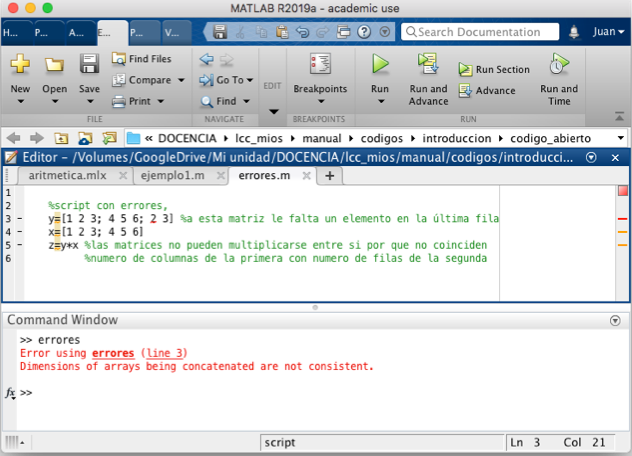
\includegraphics[width=14cm]{errores.png}
\caption{Vista de el editor de texto de Matlab. Circulo rojo error en el c�digo. Rodeado en azul advertencias de posible mejoras. Rodeado en verde mensaje de error en tiempo de ejecuci�n}
\label{fig:ederror}
\end{figure}

Si pasamos el rat�n por encima de los caract�res en rojo, Matlab nos ofrece informaci�n adicional sobre el error detectado o la advertencia de mejora. La figura \ref{fig:popupm} muestra la informaci�n asociada al error rodeado en rojo en la figura anterior (ref{fig:ederror}).

\begin{figure}[h]
\centering
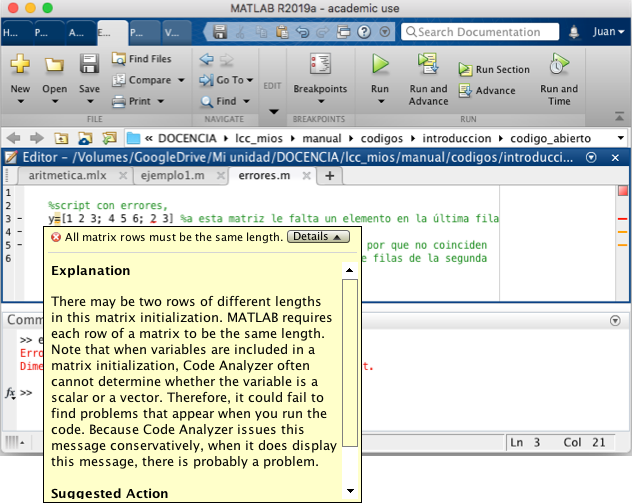
\includegraphics[width=14cm]{popupm.png}
\caption{Vista de el editor de texto de Matlab. Desplegable mostrando detalles sobre el error cometido}
\label{fig:popupm}
\end{figure}

Si ejecutamos el script, que hemos guardado con el nombre de \texttt{errores.m},

\begin{verbatim}
>> errores
Error using errores (line 3)
Dimensions of arrays being concatenated are not consistent.
\end{verbatim}

Matlab ha detectado el error en la construcci�n de la matriz \texttt{y}, nos indica mediante un mensaje el tipo de error cometido y la l�nea de c�digo donde se ha producido y detiene la ejecuci�n del \emph{script}. Se trata del mensaje rodeado en verde en la figura \ref{fig:ederror}.

Si corregimos el c�digo, a�adiendo a la matriz \texttt{y} el elemento que le falta,

\begin{lstlisting}
% script con errores,
y=[1 2 3; 4 5 6; 2 3 8] % Ultima fila completada
x=[1 2 3; 4 5 6]
z=y*x % las matrices no pueden multiplicarse entre si por que no 
      % coinciden numero de columnas de la primera con numero de
      % filas de la segunda
\end{lstlisting}
y volvemos a ejecutar el script.
\begin{verbatim}
>> errores

y =

     1     2     3
     4     5     6
     2     3     8


x =

     1     2     3
     4     5     6

Error using  * 
Incorrect dimensions for matrix multiplication. Check that the number of
columns in the first matrix matches the number of rows in the second matrix.
To perform elementwise multiplication, use '.*'.

Error in errores (line 5)
z=y*x % las matrices no pueden multiplicarse entre si por que no coinciden

\end{verbatim}
Matlab nos detecta el siguiente error cometido as� como la l�nea en la que se comete. Es interesante notar que, aunque  se trata de un error de sistaxis, el editor de textos no puede detectarlo y, por tanto, no nos muestra ning�n car�cter subrrayado en rojo, asociado a �l.

Si intercambiamos las posiciones entre las variables \texttt{x} e \texttt{y} en el producto, suponiendo que �sta es la causa del error cometido,

\begin{verbatim}
y=[1 2 3; 4 5 6; 2 3 8] 

x=[1 2 3; 4 5 6]
z=x*y 
\end{verbatim}

El c�digo se ejecuta con normalidad,
\begin{verbatim}
>> errores

y =

     1     2     3
     4     5     6
     2     3     8


x =

     1     2     3
     4     5     6


z =

    15    21    39
    36    51    90
\end{verbatim}

\item Errores de codificaci�n.\index{Errores! De codificaci�n} Este segundo tipo de errores son mucho m�s dif�ciles de detectar. El c�digo se ejecuta sin problemas, pero los resultados no son los esperados. Ante esta situaci�n, no queda m�s remedio que ir revisando el c�digo, paso a paso para detectar donde est� el error.

El siguiente c�digo del script \texttt{trect.m} muestra un error de este tipo, 

\begin{lstlisting}
% este script toma los valores de los catetos de un tri�ngulo rectangulo del 
% workspace de matlab (variables a y b). calcula su hipotenusa, y a partir
% de estos datos, el seno el coseno y la tangente del angulo formado por la
% hipotenusa y el cateto mayor que ser� siempre a

% calculo hipotenusa,

h=sqrt(a^2+b^2)

% calculo del seno

s=a/h

% calculo del coseno
a=b/h % error estamos sobreescribiendo el valor del coseno en la variable  
      % que guardaba e valor del cateto

% calculo de la tangente
t=b/a

\end{lstlisting}

%\lstinputlisting{../codigo/matlab/introduccion/trect.m}

El programa funciona perfectamente, por ejemplo si hacemos \texttt{a=4} y \texttt{b}=3,

\begin{verbatim}
>> trect

h =

     5


s =

    0.8000


a =

    0.6000


t =

     5
\end{verbatim}
Como hemos sobrescrito en \texttt{a} el valor del coseno, cuando tratamos de utilizar dicha variable como si fuera el cateto mayor para obtener la tangente, el resultado que obtenemos es err�neo.

El editor de texto de Matlab nos permite ejecutar un programa paso a paso, ver los valores que van tomando las variable en Matlab, etc, mediante el depurador que lleva incorporado. Para ello, se definen en el editor de Matlab \emph{breakpoints},esto es: l�neas en las cuales Matlab detendr� la ejecuci�n de un programa, entrar� en modo de depuraci�n y esperar� instrucciones del usuario. La figura \ref{fig:depu1} muestra el c�digo del ejemplo que acabamos de ver, en el que se ha definido un \texttt{breakpoint}, pulsando con el rat�n sobre el gui�n que precede a la l�nea del programa en la que se desea parar la ejecuci�n. Matlab indica que el \emph{breakpoint} est� activo, cambiando el gui�n por un c�rculo rojo. Alternativamente, tambi�n es posible establecer o remover \emph{breackpoints} empleando el bot�n de la pesta�a \emph{EDITOR}, rodeado de rojo en la figura.

\begin{figure}[h]
\centering
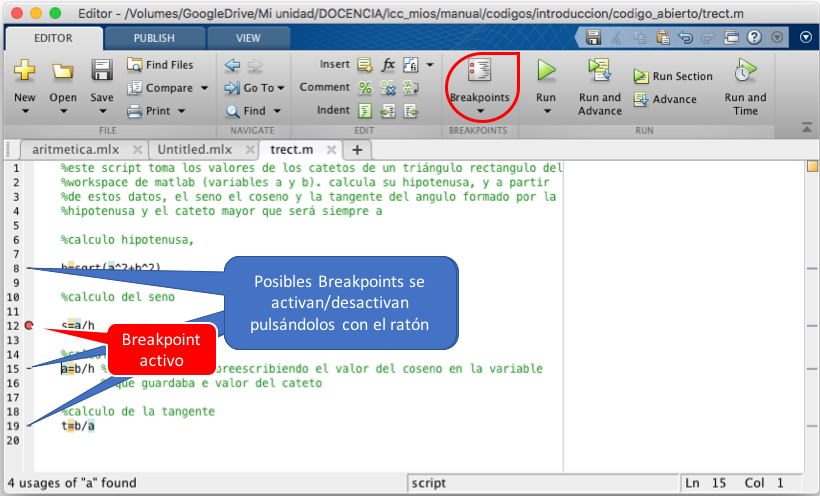
\includegraphics[width=14cm]{depu1.png}
\caption{Breakpoint activo}
\label{fig:depu1}
\end{figure}

Si una vez se�alado el \emph{breakpoint}, ejecutamos el \emph{script},
\begin{verbatim}
>> trect

h =

    3.1477

12  s=a/h
K>> 
\end{verbatim}

Matlab nos indica que ha detenido la ejecuci�n del programa en la l�nea marcada por el \emph{breakpoint} (l�nea 12 en el ejemplo). adem�s vuelve a mostrar el \emph{prompt} en la ventana de comandos, pero esta vez precedido por la letra \texttt{k}, para indicarnos que ha entrado en modo de depuraci�n.

A partir de aqu� Matlab pone a nuestra disposici�n las herramientas de depuraci�n, la figura \ref{fig:depu2} muestra la l�nea en que se ha parado la ejecuci�n del programa, se�alada con una flecha verde, y algunas de estas herraminentas. B�sicamente nos da la posibilidad de ejecutar el c�digo paso a paso, de entrar e ir paso a paso en las funciones que llama nuestro programa, o de de continuar la ejecuci�n hasta que el final del programa o hasta el siguiente \emph{breakpoint} activo. Para dominar los detalles del depurador se aconseja leer la ayuda de Matlab.


\begin{figure}[h]
\centering
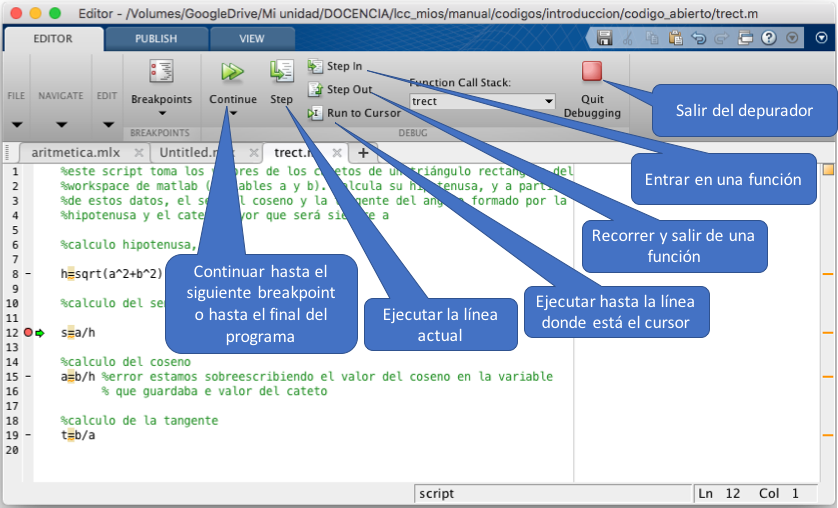
\includegraphics[width=14cm]{depu2.png}
\caption{Parada de programa en breakpoint y herramientas de depuraci�n}
\label{fig:depu2}
\end{figure}

Si pulsamos el bot�n  ``ejecutar l�nea actual'' Matlab ejecutar� la l�nea de programa se�alada con la flecha verde y se parar� en la l�nea siguiente. En cada paso, podemos ver el valor que toman las variables, pidiendo su valor directamente en la ventana de comandos,

\begin{verbatim}
K>> a

a =

    0.9531
\end{verbatim}

o bien se�alando (sin pulsar botones) con el rat�n en el editor de texto la variable de la que se trate.
En nuestro ejemplo del tri�ngulo rect�ngulo es muy sencillo avanzar paso a paso en el programa con el depurador, y caer en la cuenta que, cuando se va a calcular la tangente, la variable \texttt{a} ya no contiene el valor del cateto.

\item Advertencias. \index{Advertencias} \index{Warnning}Por �ltimo se�alar la existencia de los \emph{warnings} no se trata propiamente de errores, sino de simples advertencias de que algo puede funcionar de forma m�s eficiente, o puede no dar el resultado que esper�bamos. En general, cuando se recibe un \emph{warning} al ejecutar un programa, o cuando el editor de Matlab subraya en rojo alg�n car�cter en el editor de textos, se debe corregir el programa para que desaparezcan, aunque propiamente no se trate de errores.
\end{enumerate} 


 




\section{Control de Flujo}\index{Flujo} \index{Control de flujo}
En la secci�n anterior, se introdujo el modo de escribir programas en Matlab mediante el uso de 	\emph{scripts} y funciones. En todos los casos vistos, la ejecuci�n del programa empezaba por la primera l�nea del programa, y continuaba, por orden, l�nea tras l�nea hasta alcanzar el final del programa. Se trata de programas en los que el \emph{flujo} es lineal, porque los resultados de cada l�nea de programa se van obteniendo regularmente uno detr�s de otro. 

Hay ocasiones en las que, por diferentes razones que expondremos a continuaci�n, puede interesarnos alterar el orden en que se ejecutan las sentencias de un programa, bien repitiendo una parte de los c�lculos un determinado n�mero de veces o bien ejecutando unas partes de c�digo u otras en funci�n de que se satisfagan unas determinadas condiciones.

El control del orden en que se ejecutan las sentencias de un programa es lo que se conoce con el nombre de \emph{control de flujo}. Veremos dos tipos principales de control de flujo: El flujo condicional y los bucles.
\subsection{Flujo condicional.}\index{Flujo!Condicional}
Empezaremos con un ejemplo sencillo de c�mo y para qu� condicionar el flujo de un programa. Supongamos que queremos construir un programa que reciba como variable de entrada un n�mero cualquiera y nos muestra un mensaje por pantalla si el n�mero es par.

Para ello, podr�amos hacer uso de la funci�n \texttt{rem} (ver tabla \ref{tabfun}). Si el resto de la divisi�n entre dos del n�mero suministrado a la funci�n es cero, se trata de un n�mero par; si no, es un n�mero impar. Podr�amos hacer uso de operadores relacionales, en particular de \texttt{==} para comprobar si el resto de la divisi�n entre dos es cero. Por �ltimo necesitar�amos alg�n mecanismo que permitiera al programa escribir un mensaje solo cuando el n�mero introducido sea par.

\paragraph{if - elseif - else - end.} El mecanismo que necesitamos nos lo suministra la estructura \texttt{if} de Matlab. Veamos en primer lugar el c�digo del ejemplo del que venimos hablando,

\begin{lstlisting}
function espar(x)
% Este programa recibe un numero entero como variable de entrada. y muestra
% por pantalla un mensaje indicando si el numero recibido es par o impar.

% Calculamos el resto de la division por dos
resto=rem(x,2);

% Empleamos una estructura if - else -end para decidir que mensaje mostrar

if resto==0
    % si el resto es cero el n�mero es par
    disp('el n�mero es par')
end
\end{lstlisting}

El programa toma un n�mero como variable de entrada y calcula el resto de su divisi�n entre dos. A continuaci�n entra en una parte de c�digo especial, que se inicia con la palabra clave \texttt{if} y termina con la palabra clave \texttt{end}. 

La palabra clave \texttt{if} va siempre seguida de una expresi�n que da un resultado l�gico: verdadero ($1$) o falso ($0$). Esta expresi�n puede ser cualquier combinaci�n v�lida de expresiones relacionales o l�gicas. Esta expresi�n l�gica, que sigue al if constituye una condici�n. El programa seguir� ejecutando las siguientes l�neas solo si la condici�n se cumple; si no, se las saltar� hasta llegar a la expresi�n \texttt{end}.

En nuestro ejemplo, se emplea una expresi�n relacional sencilla \texttt{resto==0}. Si se cumple, el programa ejecutar� la siguiente l�nea de programa, escribiendo en la ventana de comandos la frase ``el n�mero es par"  si no se cumple el programa se la salta, llega hasta el \texttt{end}, y no escribe nada por pantalla. 

Acabamos de ver la estructura condicional \texttt{if} m�s sencilla posible. Podr�amos complicarla un poco pidiendo que tambi�n nos saque un mensaje por pantalla cuando el n�mero sea impar. Esto supone incluir en nuestro programa una disyuntiva; si es par el programa debe hacer una cosa y si no, debe hacer otra. Para incluir este tipo de disyuntivas en una estructura \texttt{if}, se emplea la palabra clave \texttt{else}. Veamos nuestro ejemplo modificado,
\begin{lstlisting}
function espar(x)
% Este programa recibe un numero entero como variable de entrada. y muestra
% por pantalla un mensaje indicando si el numero recibido es par o impar.

% Calculamos el resto de la division por dos
resto=rem(x,2);

% Empleamos una estructura if - else -end para decidir que mensaje mostrar

if resto==0
    % si el resto es cero el n�mero es par
    disp('el n�mero es par')
else
    % si el resto no es cero el n�mero es impar
    disp('el n�mero es impar')
end 
\end{lstlisting}

La palabra clave \texttt{else} marca ahora la disyuntiva, si el n�mero es par, el programa ejecuta las l�neas de c�digo entre el \texttt{if} y el \texttt{else}, si el n�mero no es par ejecutar� las l�neas entre el \texttt{else} y el \texttt{end}.

La estructura \texttt{if} admite todav�a ampliar el n�mero de posibilidades de elecci�n mediante la palabra clave \texttt{elseif}. Al igual que  con \texttt{if}, \texttt{elseif} va seguido de una expresi�n l�gica que establece una condici�n, si se cumple se ejecutar� el c�digo de las l�neas siguientes, si no se cumple, el programa saltar� a la siguiente l�nea que contenga una palabra clave: otro \texttt{elseif}, un \texttt{else} o directamente el \texttt{end} que marca el final de la parte de c�digo condicional. Para ver c�mo funciona, vamos a modificar nuestro ejemplo anterior, para que, si el n�mero introducido no es divisible por dos, compruebe si es divisible por tres,

\begin{lstlisting}
function divis(x)
% Este programa recibe un numero entero como variable de entrada. y muestra
% por pantalla un mensaje indicando si el numero recibido es par. Si no 
% es par, comprueba si es divisible por 3 y si lo es muestra un mensaje   
% por pantalla indicandolo. Si no es par ni divisible por tres muestra un
% mensaje diciendo que no es par ni disible por tres. 



% Empleamos una estructura if-elseif-else-end para decidir que mensaje mostrar

if rem(x,2)==0
    % si el resto es cero el n�mero es par
    disp('el n�mero es par')
elseif rem(x,3)==0
    % El n�mero es divisible por tres
    disp('el n�mero es divisible por 3')
else
    % el numero no es par ni divisible por tres
    disp('el n�mero no es par ni divisible por 3')
end
\end{lstlisting}

Si llamamos ahora a la funci�n dando como valor de entrada un n�mero par, Ejecutar� el c�digo situado debajo del \texttt{if} y antes del \texttt{elseif} y se saltar� todo lo dem�s hasta llegar al \texttt{end}. Si el n�mero introducido no es par, pero es divisible por tres, se saltar� el c�digo situado por debajo del \texttt{if}, ejecutar� el c�digo contenido debajo del \texttt{elseif} hasta el \texttt{else} y saltar� el resto del c�digo hasta llegar al \texttt{end}. Por �ltimo si el n�mero no es par ni divisible por tres, solo ejecutar� el c�digo situado por debajo del \texttt{else}.

Un aspecto que debemos resaltar, es que el programa ejecutar� el c�digo correspondiente a la primera condici�n que se cumpla, y se saltar� el resto hasta llegar al \texttt{end}. As� por ejemplo, si en nuestro ejemplo introducimos el n�mero $6$, el programa nos mostrar� el mensaje ``el n�mero es par", puesto que �sta es la primera condici�n que se cumple, pero nunca nos mostrar� el mensaje ``el n�mero es divisible por 3". Porque una vez comprobada y cumplida la primera condici�n (ser par) el programa salta directamente al \texttt{end} final de la estructura, sin comprobar nada m�s. La figura \ref{fig:if} muestra el esquema completo de una estructura \texttt{if}. Los t�rminos entre par�ntesis pueden estar o no presentes en una implementaci�n concreta.

\begin{figure}[h]
\centering
\begin{tikzpicture}
%\usetikzlibrary{shapes.multipart}
\path (5,0) node(a) [rectangle split,rectangle split parts =2,draw=blue,top color=white,bottom color=blue!15, very thick,align=left,rounded corners]{Estructura if-elseif-else-end
\nodepart{two}

if condici�n\\
\ \ \ ... c�digo\\
\ \ \ ...\\
(elseif condici�n)\\
\ \ \ ... c�digo\\
\ \ \ ...\\
(elseif condici�n)\\
\ \ \ ... c�digo\\
\ \ \ ...\\
.\\
(puede haber tantos bloques elseif como se necesiten)\\
.\\
(else)\\
\ \ \ ... c�digo\\
\ \ \ ...\\
end};		
\end{tikzpicture}
\caption{Esquema general de la estructura de flujo condicional \texttt{if} los t�rminos escritos entre par�ntesis son opcionales.}
\label{fig:if}
\end{figure} 

\paragraph{Estructuras if anidadas.}\index{Anidaci�n! If anidado} 
En el ejemplo anterior, hemos visto c�mo, si el n�mero introducido en la funci�n era par y adem�s divisible por tres, el programa nunca nos informar�a de esta segunda propiedad, debido al car�cter excluyente de la estructura \emph{if}. Una manera de resolver este problema, es mediante el uso de estructuras \texttt{if} anidadas. La idea es muy sencilla, se construye una estructura \texttt{if} para comprobar una determinada condici�n, si esta se cumple, dentro de su c�digo se construye otra estructura if para comprobar una segunda condici�n, y as� sucesivamente, todas las veces que sea necesario. Si modificamos nuestro ejemplo anterior, incluyendo un \texttt{if} anidado,

\begin{lstlisting}
function divis23(x)
% Este programa recibe un numero entero como variable de entrada. y 
% muestra por pantalla un mensaje indicando si el numero recibido es par. 
% si el numero es par y divisible entre tres,
% si es divisible entre tres  
% Si no es par ni divisible por tres 



% Empleamos una estructura if - else -end 
% y un if anidado para decidir que mensaje mostrar

if rem(x,2)==0
    % si el resto es cero el n�mero es par
    % comprobamos con un if anidado si adem�s es divisible entre tres
    if rem(x,3)==0
        disp('el n�mero es par y divisible entre tres')
    else
        disp('el n�mero es par')
    end
elseif rem(x,3)==0
    % El n�mero es divisble entre tres
    disp('el n�mero es divisible entre 3')
else
    % el numero no es par ni divisible entre tres
    disp('el n�mero no es par ni divisible entre tres')
end
\end{lstlisting}

\paragraph{Switch-case-otherwise.} \index{Flujo! Switch-case}Se trata de otra estructura que permite tambi�n ejecutar una parte u otra de c�digo de acuerdo con unas codiciones preestablecida. Estas condiciones se presentan en forma de \emph{casos}, el programa comprueba al llegar a la estructura \texttt{switch} de qu� caso se trata y ejecuta el c�digo correspondiente. La figura \ref{fig:switch} muestra la forma general que toma una estructura \texttt{switch}.

La estructura \texttt{switch}, compara el valor contenido en la variable de entrada a la estructura con las expresiones contenidas en los casos, ejecutando el primer caso para el que coincidan. Si no encuentra ninguno, ejecuta entonces el c�digo contenido debajo de la sentencia \texttt{otherwise}.

Veamos un ejemplo muy sencillo,

\begin{lstlisting}
function signo(x)
% este programa emplea una estructura switch para informarnos del signo de
% un n�mero.

% NOTA EL PROGRAMA NO COMPRUEBA QUE LA VARIABLE DE ENTRADA X SEA UN NUMERO,
% SI ES UN VECTOR O UNA MATRIZ EL RESULTADO NO TIENE SENTIDO
  
s=sign(x); % obtnemos el signo del n�mero mediante la funci�n sign

% construimos la estructura switch,

switch s
    case 1
        disp('el n�mero es positivo')
    case -1
        disp('el n�mero es negativo')
    otherwise
        disp('el n�mero es cero')
end

\end{lstlisting}

\begin{figure}[h]
\centering
\begin{tikzpicture}
%\usetikzlibrary{shapes.multipart}
\path (5,0) node(a) [rectangle split,rectangle split parts =2,draw=green,top color=white,bottom color=green!20, very thick,align=left,rounded corners]{Estructura switch-case-otherwise
\nodepart{two}
switch variable\\
\ \ \ case expresi�n\\
\ \ \ \ \ ... c�digo\\
\ \ \ case expresi�n\\
\ \ \ \ \ ... c�digo\\
\ \ \ .\\
Puede haber tantos bloques \emph{case} como se necesiten\\
\ \ \ .\\
\ \ \ otherwise\\
\ \ \ \ \ ... c�digo\\
end};		
\end{tikzpicture}
\caption{Esquema general de la estructura switch-case-otherwise}
\label{fig:switch}
\end{figure}

La funci�n del ejemplo emplea a su vez la funci�n de Matlab \texttt{sign} para obtener el signo ($1$, $-1$, $0$) del n�mero introducido. Guarda el resultado de esta operaci�n en la variable \texttt{s}, que ser� precisamente la variable de entrada a la estructura \texttt{switch}. Los casos se limitan a chequear los posibles valores de la variable y enviar a la ventana de comandos el mensaje correspondiente.
 
\subsection{Bucles}\index{Flujo!Bucles}\index{Bucles}
En ocasiones, es preciso repetir una operaci�n un n�mero determinado de veces o hasta que se cumple una cierta condici�n. Los lenguajes de alto nivel poseen estructuras espec�ficas, para repetir la ejecuci�n de un trozo de programa las veces que sea necesario. Cada repetici�n recibe el nombre de iteraci�n. Estas estructuras reciben el nombre gen�rico de bucles. Vamos a ver dos tipos: los bucles \texttt{for} y los bucles \texttt{while}.

\paragraph{Bucles for.} \index{Flujo! Bucle for}\index{Bucles! Bucle for}Un bucle \texttt{for} repite las sentencias contenidas en el bucle un determinado n�mero de veces, es decir realiza un n�mero fijo de iteraciones. La estructura general de un bucle \texttt{for} se muestra en la figura, \ref{fig:for}

\begin{figure}[h]
\centering
\begin{tikzpicture}
%\usetikzlibrary{shapes.multipart}
\path (5,0) node(a) [rectangle split,rectangle split parts =2,draw=orange,top color=white,bottom color=orange!30, very thick,align=left,rounded corners]{Estructura de un bucle for
\nodepart{two}

for indice=[vector de valores]\\
\ \ \ ... c�digo\\
(condici�n: Break)\\
\ \ \ ...\\
(condicici�n: Continue)\\
\ \ \ ... c�digo\\

end};		
\end{tikzpicture}
\caption{Esquema general de la estructura de un bucle \texttt{for} los t�rminos escritos entre par�ntesis son opcionales.}
\label{fig:for}
\end{figure} 
 
El bucle empieza con la palabra clave for, seguida de una variable a la que hemos dado el nombre gen�rico de �ndice. Esta variable ir� tomando sucesivamente los valores de los elementos contenidos en el [vector de valores]. El c�digo contenido en el bucle, desde la l�nea siguiente al \texttt{for} hasta el \texttt{end} se ejecutar� tantas veces como valores tenga el vector de valores. Antes de hablar de las sentencias \texttt{break} y \texttt{continue}, veamos alguno ejemplos.
\begin{lstlisting}
function y=demofor(x)
% este programa emplea un bucle for sencillo para ir mostrando uno 
% a uno los elementos del vector de entrada x por pantalla. adem�s  
% los suma y guarda el resultado total en el vector y,

y=0; % iniciamos la suma a cero

for i=x
    disp(i)
    y=y+i;
end
\end{lstlisting}

Si ejecutamos el programa, usando como entrada el vector \texttt{d=[1 9 4 18]},

\begin{verbatim}
>> d=[1 9 4 18]

d =

     1     9     4    18

>> suma=demofor(d)
     1

     9

     4

    18


suma =

    32
\end{verbatim}

Una vez que el programa llega al bucle \texttt{for}, iguala la variable \texttt{i} al primer valor contenido en el vector de entrada, lo muestra por pantalla y a�ade su valor a la variable de salida. cuando llega al \texttt{end} del bucle for comprueba que todav�a quedan valores del vector de entrada por recorrer, as� que vuelve al principio del \texttt{for}, igual la variable \texttt{i} al segundo valor del vector de entrada, suma dicho valor a la variable de salida, llega al \texttt{end} y as� sucesivamente hasta que haya recorrido todos los valores del vector de entrada.

El uso m�s habitual de los bucles, es para recorrer elementos de un vector o de una matriz. por esta raz�n, lo m�s frecuente es que no se de expl�citamente el vector cuyos elementos debe recorrer el �ndice del \texttt{for}, sino que se construya empleado el operador \texttt{:},
\begin{verbatim}
for indice=principio:incremento:final
\end{verbatim}

Veamos un ejemplo sencillo para obtener el vector suma de dos vectores,
\begin{lstlisting}
function s=sumafor(x,y)
% este programa emplea un bucle for sencillo para sumar dos vectores
% primero comprueba si son del mismo tama�o. Si no lo son da un mensaje 
% de aviso

l1=length(x);
l2=length(y);
if l1==l2
    % construimos un vector de ceros del mismo tama�o que x e y paraa
    % guardar el resultado de la suma,
    s=zeros(size(x));
    % si son iguales los suma elemento a elemento usando un bucle for
    for i=1:l1
        s(i)=x(i)+y(i);
    end
else
    disp('los vectores son de distinto tama�o')
end
\end{lstlisting}

En la figura \ref{fig:for}, aparecen dos sentencias opcionales, \texttt{break} y \texttt{continue}.

La sentencia \texttt{break}, permite terminar el bucle \texttt{for} antes de que haya terminado de realizar todas las ejecuciones previstas. La sentencia break va siempre incluida dentro de una condici�n que, si se cumple interrumpe la ejecuci�n del bucle. Por ejemplo, podemos emplear un bucle \texttt{for} y una sentencia \texttt{break}, para buscar la primera vez que un determinado n�mero aparece en un vector,

\begin{lstlisting}
function posicion=buscanum(x,n)
% este programa emplea un bucle for y un break para buscar en el  
% vector x, la primera vez que aparece el n�mero n

% obtenemos la longitud del vector
l1=length(x);
% iniciamos la variable posicion a un valor absurdo
posicion=-1;
for i=1:l1
    if x(i)==n
        posicion=i:
        break
    end
end
if posicion==-1
    disp('el numero pedido no se encuentra en el vector x') 
end
\end{lstlisting} 

El programa toma como variables de entrada un vector y el n�mero que debe buscar dentro del vector. Construye un bucle \texttt{for}, con el mismo n�mero de iteraciones que el tama�o del vector. El bucle va comparando los elementos del vector con el n�mero pedido. Cuando encuentra un elemento igual, se ejecuta el c�digo de la estructura if contenida en el bucle; la variable posici�n toma el valor del �ndice \texttt{i} del bucle y la sentencia \texttt{break} interrumpe la ejecuci�n del bucle, saltando al final del mismo. Por �ltimo, se ha a�adido una condici�n al terminar el bucle, para el caso de que se hayan recorrido todos los elementos del vector sin encontrar el n�mero pedido.

La sentencia \texttt{continue}, se emplea para hacer que una determinada iteraci�n interrumpa su ejecuci�n y salte directamente al comienzo de la siguiente iteraci�n. Debe ir, como en el caso de la sentencia \texttt{break}, incluida en una estructura condicional. Veamos un ejemplo para entender como funciona. Se trata de un programa que admite como entrada un vector de cualquier longitud y devuelve como salida otro vector que contiene solo los n�meros pares contenidos en el vector de entrada,

\begin{lstlisting}
function pares=buscapar(x)
% este programa emplea un bucle for y un continue para construir un 
% vector de salida con los numeros pares contenidos en el vector de entrada.

% obtenemos la longitud del vector
l1=length(x);
% iniciamos el vector de salida a un vector vac�o,
pares=[];
for i=1:l1
    if rem(x(i),2)~=0
        continue
    end
    pares=[pares x(i)];
end
\end{lstlisting}

El funcionamiento es muy sencillo, en cada iteraci�n la sentencia \texttt{if} comprueba si el n�mero es par. Si no lo es, entra en el c�digo de la estructura \texttt{if}, ejecuta la sentencia \texttt{continue}, y se salta el resto del c�digo del bucle, volviendo directamente a empezar la siguiente iteraci�n.

\paragraph{bucles for anidados.} \index{Anidaci�n!For anidado}Los bucles \texttt{for} pueden anidarse unos dentro de otros de modo an�logo a como se hace con las estructuras \texttt{if}. Veamos un ejemplo de uso, muy com�n; calcular la suma de dos matrices,

\begin{lstlisting}
function s=suma_mat(x,y)
% este programa emplea dos bucles for anidados para obtener la suma de 
% dos matrices.

% obtenemos el tama�o de las matrices,
t1=size(x);
t2=size(y);
if t1(1)==t2(1)&& t1(2)==t2(2)
    % si las matrices tienen el mismo tama�o pueden sumarse...
    % construimos una matriz de dicho tama�o para guardar el 
    % resultado de la suma
    s=zeros(size(x));
    % construimos un bucle que recorre las filas de ambas matrices
    for i=1:t1(1)
        % y dentro, anidamos un bucle que recorre las columnas
        for j=1:t1(2)
            % Empleando ambos �ndices para ir sumando los elementos 
            % de las dos matrices,
            s(i,j)=x(i,j)+y(i,j);
        end
    end
else
    % si no tienen el mismo tama�o no se pueden sumar...
    disp('las matrices no son del mismo tama�o')
end
\end{lstlisting} 

Es interesante observar en este ejemplo el funcionamiento de los dos bucles anidados. Cada interaci�n del bucle exterior, avanza una fila, en el recorrido de las matrices, cada iteraci�n del bucle interior recorre todos los elementos de la fila indicada por el bucle exterior.

\paragraph{bucle while.} \index{Flujo! Bucle while}\index{Bucles! Bucle while} Este bucle tiene la misma finalidad que un bucle \texttt{for}, repetir un trozo de c�digo un determinado n�mero de veces. Lo que cambia, es el mecanismo que determina cuantas iteraciones realizar� el bucle. En el caso de un bucle \texttt{while} las iteraciones se repiten un n�mero indefinido de veces mientras se cumpla una determinada condici�n impuesta al principio del bucle. La figura \ref{fig:while} muestra la estructura general de un bucle while.

\begin{figure}[h]
\centering
\begin{tikzpicture}
%\usetikzlibrary{shapes.multipart}
\path (5,0) node(a) [rectangle split,rectangle split parts =2,draw=yellow,top color=white,bottom color=yellow!40, very thick,align=left,rounded corners]{Estructura de un bucle while
\nodepart{two}

while condici�n\\
\ \ \ ... c�digo\\
(condici�n: Break)\\
\ \ \ ...\\
(condicici�n: Continue)\\
\ \ \ ... c�digo\\
end};		
\end{tikzpicture}
\caption{Esquema general de la estructura de un bucle \texttt{while} los t�rminos escritos entre par�ntesis son opcionales.}
\label{fig:while}
\end{figure}

Veamos un ejemplo sencillo. 

\begin{lstlisting}
function n=potencia(x,max)
% este programa emplea un bucle while para calcular la potencia a 
% la que hay que elevar un n�mero x para que el resultado sea mayor 
% que otro determinado n�mero max
% un n�mero.

% NOTA EL PROGRAMA NO COMPRUEBA QUE LA VARIABLE DE ENTRADA X SEA UN NUMERO,
% Si ES UN VECTOR O UNA MATRIZ EL RESULTADO NO TIENE SENTIDO
  
pot=1;
n=0;
while pot<max % mientras la potencia calculada sea menor que max
    n=n+1;
    pot=x^n;
end
\end{lstlisting}

El programa emplea un bucle \texttt{while} para calcular el exponente m�nimo al que hay que elevar un n�mero para que rebase una determinada cantidad. El bucle while se ejecuta mientras la potencia calculada sea menor que la variable \texttt{max}; una vez que la potencia rebasa dicho valor el bucle deja de ejecutarse. Un aspecto muy importante del bucle \texttt{while} es que al programarlo hay que asegurarse de que dentro del bucle existe la posibilidad de cambiar la condici�n de entrada. Si no, el programa no podr� terminar nunca el bucle\footnote{Cuando se produce esta situaci�n por un error en el dise�o del programa, el bucle se puede parar pulsando a la vez las teclas ctrl+c}.

Las sentencias \texttt{break} y \texttt{continue} son id�nticas a las descritas en el caso de los bucles \texttt{for}, por lo que no insistiremos m�s sobre el asunto.

\paragraph{Bucles while anidados.} \index{Anidaci�n! While anidado} Del mismo modo que se anidan los bucles \texttt{for}, es posible anidar bucles \texttt{while}. Como un ejemplo, vamos a reproducir el programa desarrollado antes para sumar dos matrices, empleando ahora bucles \texttt{while}.

\begin{lstlisting}
function s=suma_while(x,y)
% este programa emplea dos bucles while anidados para obtener la 
% suma de dos matrices.

% obtenemos el tama�o de las matrices,
t1=size(x);
t2=size(y);
if t1(1)==t2(1)&& t1(2)==t2(2)
    % si las matrices tienen el mismo tama�o pueden sumarse...
    % construimos una matriz de dicho tama�o para guardar el 
    % resultado de la suma
    s=zeros(size(x));
    % construimos un bucle que recorre las filas de ambas matrices
    i=1; % inicimos un contador para las filas
    while i<=t1(1)
        % y dentro, anidamos un bucle que recorre las columnas
        j=1; % iniciamos un contador para las columnas
        while j<=t1(2)
            % Empleando ambos �ndices para ir sumando los elementos 
            % de las dos matrices,
            s(i,j)=x(i,j)+y(i,j);
            j=j+1; % vamos incrementando el indice de columnas
        end
        i=i+1; % vamos incrementando el indice de filas
    end
else
    % si no tienen el mismo tama�o no se pueden sumar...
    disp('las matrices no son del mismo tama�o')
end
\end{lstlisting}

El ejemplo, es m�s complicado de programar y menos eficiente que si us�ramos bucles \texttt{for}. La raz�n de incluirlo es puramente ilustrativa. En general, un bucle \texttt{while} debe utilizarse solo cuando el n�mero de iteraciones que se precisa realizar no es fijo, sino que depende de alguna condici�n propia de los resultados que se van obteniendo a medida que se van realizando iteraciones.

\subsection{Funciones recursivas.} \index{Funciones! Recursivas}
Una funci�n recursiva es una funci�n que se llama a s� misma. Hemos esperado hasta aqu� para hablar de ellas porque, de alguna manera, se comportan como un bucle y necesitan una condici�n de salida para dejar de llamarse a s� mismas y terminar su ejecuci�n. En general, son delicadas de manejar y tienden a consumir mucha memoria ya que cada vez que la funci�n se llama a s� misma necesita crear un nuevo espacio de memoria independiente. Veamos un ejemplo de funci�n recurrente que permite obtener el t�rmino en�simo de la sucesi�n de Fibonacci  
\begin{align*}
f_0=0, f_1=1, f_2=1, f_3=2, f_4=3, f_5=5, f_6=8, \cdots f_i=f_{i-1}+f_{i-2} \cdots 
\end{align*}

La sucesi�n empieza con los t�rminos $0$ y $1$ y a partir de ah� cada t�rmino es la suma de los dos anteriores. Podemos convertir directamente esta definici�n en c�digo,

\lstinputlisting{../codigo/matlab/introduccion/fibonacci.m}

Si n es menor que dos, la funci�n da como valor el t�rmino correspondiente (1 o 0). Si n es mayor que dos, vuelve a llamarse a si misma con entrada \texttt{n-1} y \texttt{n-2}, para calcular el valor en�simo de la sucesi�n a partir de la suma de los dos anteriores, la funci�n se ir� llamando a s� misma hasta  llegar a $n<2$. A partir de ah� ira devolviendo los valores obtenidos en cada llamada hasta obtener el en�simo t�rmino.

\subsection{Algoritmos y diagramas de flujo.} \index{Flujo! Diagrama de Flujo}
Un algoritmo es, en la definici�n de la Real Academia: 
\begin{quotation}
Un conjunto ordenado y finito de operaciones que permite hallar la soluci�n de un problema.
\end{quotation}

La palabra algoritmo ha llegado hasta nosotros transcrita del nombre del matem�tico �rabe \emph{Al-Juarismi} (circa 780-850 dc). En programaci�n los algoritmos son importantes, porque suponen un paso previo a la creaci�n de un programa.

Habitualmente, partimos de un problema para el que tenemos un enunciado concreto. Por ejemplo: obtener los $n$ primeros n�meros primos. 

El siguiente paso, ser�a pensar y definir un algoritmo que permita resolver nuestro problema, es importante caer en la cuenta de que un mismo problema puede resolverse, en muchos casos, por distintos caminos. Por tanto es posible dise�ar distintos algoritmos para resolver un mismo problema. Un posible algoritmo para el problema de los n�meros primos ser�a el siguiente,

\begin{itemize}
\item Considerar 2 como el primer n�meros primo. (un n�mero primo es aquel que solo es divisible por si mismo o por uno.)
\item Recorrer todos los n�meros impares desde 3 hasta que se complete el n�mero $n$ de n�meros primos solicitados.
\item Para cada n�mero, probar a dividirlo por todos los primos obtenidos hasta ese momento. Si no es divisible por ninguno, el n�mero es primo y se guarda, si es divisible por alguno de ellos, se interrumpe el proceso y se prueba con el siguiente.
\end{itemize}

En ocasiones, facilita la comprensi�n de un algoritmo representarlo gr�ficamente mediante un diagrama de flujo. Los diagramas de flujo emplean s�mbolos bien definidos para representar los distintos paso de un algoritmo y flechas para indicar la relaci�n entre ellos; la relaci�n en la que la informaci�n \emph{fluye} de un paso del algoritmo a otro.

No hay una norma r�gida para realizar un diagrama de flujo, el grado de detalle con que se describe el algoritmo va en funci�n de las necesidades del programador, o de los destinatarios a quienes va dirigido el diagrama. La idea fundamental es que facilite la comprensi�n del algoritmo. Se utilizan diversos s�mbolos para indicar, procedimientos, condiciones, almacenamiento de resultados, etc. La figura \ref{fig:flujo} muestra los tres s�mbolos m�s empleados.

\begin{figure}[h]
\centering
\begin{tikzpicture}
%\usetikzlibrary{shapes.geometric}
\path (5,0) node(a) [ellipse,draw=blue, very thick,align=center]{Inicio y fin del algoritmo}
(5,-2) node(b)[rectangle,draw=blue, thick,rounded corners,align=center]{procedimentos}
(5,-4) node(c)[diamond,aspect=3,draw=red,thick]{flujo condicional};
\end{tikzpicture}
\caption{S�mbolos empleados en diagramas de flujo}
\label{fig:flujo}
\end{figure}

Para indicar el inicio y el fin de un algoritmo se emplea como s�mbolo una elipse. Para indicar un procedimiento concreto, como por ejemplo realizar un c�lculo, asignar un valor a una variable, etc, se emplea como s�mbolo un rect�ngulo. Por �ltimo se emplea un rombo como s�mbolo, para representar una condici�n.

Los s�mbolos se relacionan mediante flechas que indican el sentido en que se ejecuta el algoritmo. los rombos suelen tener dos flechas de salida marcadas con las palabras ``si'' y ``no'', para indicar por donde sigue el flujo de informaci�n dependiendo de si la condici�n representada se cumple o no.

Por �ltimo un bucle se representa habitualmente mediante una flecha que devuelve el flujo a un s�mbolo ya recorrido anteriormente. 

\begin{figure}
\centering
\begin{tikzpicture}
%\usetikzlibrary{shapes.geometric}
\path (6,0) node(a) [ellipse,draw=blue, very thick,align=center]{inicio}
(6,-1.5) node(b)[rectangle,draw=blue, thick,rounded corners,align=center]{Introducir cuantos\\
n�meros primos se desea obtener ($n$)}
(6,-3) node(c)[rectangle,draw=blue, thick,rounded corners,align=center]{guardar el n�mero $2$\\
como primer n�mero primo}
(6,-5) node(d)[diamond,aspect=3,draw=red,align=center,thick]{�Se ha alcanzado\\ la cifra pedida de primos?}
(11,-5) node(e)[ellipse,draw=blue,align=center,very thick]{fin}
(6,-7) node(f)[rectangle,draw=blue, thick,rounded corners,align=center]{tomar el siguiente n�mero impar}
(6,-8.3) node(g)[rectangle,draw=blue, thick,rounded corners,align=center]{tomar el primer numero primo\\ de los ya encotrados}
(6,-10.5) node(h)[diamond,aspect=3,draw=red,align=center,thick]{�Es divisible el impar entre el primo?}
(6,-13.5) node(i)[diamond,aspect=3,draw=red,align=center,thick]{�Se han acabado\\ los n�meros primos\\ ya encontrados?}
(6,-16) node(j)[rectangle,draw=blue,thick,rounded corners,align=center]{Tomar el siguinte n�mero primo\\ de la lista de los ya encontrados}
(0,-13.5) node(k)[rectangle,draw=blue,thick,rounded corners,align=center]{a�adir el n�mero\\ impar a la lista de\\ primos encontrados};
\draw[blue,-latex](a.south)--(b);
\draw[blue,-latex](b.south)--(c);
\draw[blue,-latex](c.south)--(d);
\draw[blue,-latex](d.east)--node[auto]{Si}(e);
\draw[blue,-latex](d.south)--node[auto]{No}(f);
\draw[blue,-latex](f.south)--(g);
\draw[blue,-latex](g.south)--(h);
\draw[blue,-latex](h.west)|-node[auto]{s�}(1,-10.5)|-(f);
\draw[blue,-latex](h.south)--node[auto]{no}(i);
\draw[blue,-latex](i.west)--node[auto]{s�}(k);
\draw[blue,-latex](k.north)|-(0,-5)|-(d);
\draw[blue,-latex](i.south)--node[auto]{no}(j);
\draw[blue,-latex](j.east)|-(11,-16)|-(h);
\end{tikzpicture}
\caption{Diagrama de flujo para el problema de los n�meros primos}
\label{fig:primos}
\end{figure}

La figura \ref{fig:primos} muestra un posible diagrama de flujo para el problema de los n�meros primos. Como puede observarse, contiene m�s informaci�n que la versi�n que hemos dado del algoritmo descrito con palabras. 

Las l�neas que marcan los flujos de informaci�n nos indican que ser� necesario implementar un bucle exterior hasta que se complete el n�mero $n$ de primos solicitados y un bucle interior que deber� comprobar si cada nuevo n�mero impar que probamos, es divisible por los n�meros primos encontrados hasta ese momento.

Hay una tercera condici�n que debe interrumpir la comprobaci�n para el primer n�mero primo que resulte ser divisor del n�mero que se est� comprobando.

Es f�cil extraer del diagrama de flujo las estructuras de programaci�n que necesitaremos para elaborar un c�digo que nos permita resolver el problema planteado. Por ejemplo, parece l�gico implementar el bucle exterior empleando un bucle \texttt{while}, implementar el bucle interior con un \texttt{for}, que de tantas iteraciones como primos se han encontrado hasta ese momento, Emplear un \texttt{break} para interumpir la comprobaci�n, etc.

Por supuesto es posible realizar un diagrama de flujo m�s detallado, en el que incluso se incluya expl�citamente parte del c�digo que se va a utilizar. Por ejemplo se podr�a indicar que se emplear� la funci�n \texttt{rem} para comprobar si un n�mero es divisble entre otro. Sin embargo, hay que tener cuidado para evitar que un exceso de detalle dificulte entender la l�gica del algoritmo contenida en el diagrama.

Por �ltimo el algoritmo se codifica dando lugar a un programa de ordenador que permite resolver el problema. Para ello, hay que identificar las instrucciones del algoritmo con estructuras de programaci�n validas: bucles, condicionales, etc. Veamos un posible c�digo para generar n�meros primos, siguiendo el algoritmo descrito. 
 
 \lstinputlisting{../codigo/matlab/introduccion/primos.m}
\section{Representaci�n Gr�fica}\index{Gr�ficos}
La posibilidades gr�ficas constituyen, junto a la facilidad para manejar matrices, uno de los aspectos m�s atractivos de Matlab como herramienta de c�lculo cient�fico. Matlab permite realizar gr�ficos en dos y tres dimensiones de muy diversos tipos. 

\subsection{El comando plot y las figuras en Matlab.}\index{Gr�ficos!Plot}
\paragraph{plot.} El comando de dibujo m�s sencillo de Matlab es el comando \texttt{plot}. La filosof�a de dibujo es muy sencilla se pasan como variables de entrada dos vectores, el primero de ellos con las coordenadas \texttt{x} y el segundo con las correspondientes coordenadas \texttt{y} de los puntos que se desea dibujar. Si no se indica nada, Matlab unir� los puntos mediante l�neas rectas. Supongamos que deseamos representar gr�ficamente los puntos $(x,y)$ de la siguiente tabla de datos,

\begin{table}[h]
\caption{Datos de prueba}
\centering
\begin{tabular}{|c|c|}
x&y\\ 
\hline
0&0\\
2&3\\
-1&2\\
-2&-4\\ 
\end{tabular}
\label{tpuntos}
\end{table} 

Para ello, lo primero que hacemos es construir dos vectores; uno con las coordenadas x de los puntos,
\begin{verbatim}
>> x=[0 2 -1 -2]
x =

     0     2    -1    -2

\end{verbatim}
y el otro con las coordenadas y de los puntos,
\begin{verbatim}
>> y=[0 3 2 -4]
y =

     0     3     2    -4
\end{verbatim}
 
Por �ltimo empleamos el comando \texttt{plot}, dando como variables de entrada los dos vectores construidos,
 
\begin{verbatim}
>> plot(x,y)
\end{verbatim}

Matlab responde al comando abriendo una ventana gr�fica, como la que muestra la figura \ref{fig:ventana}, con la figura correspondiente a los puntos de la tabla, unidos mediante l�neas rectas.

\begin{figure}[h]
\centering
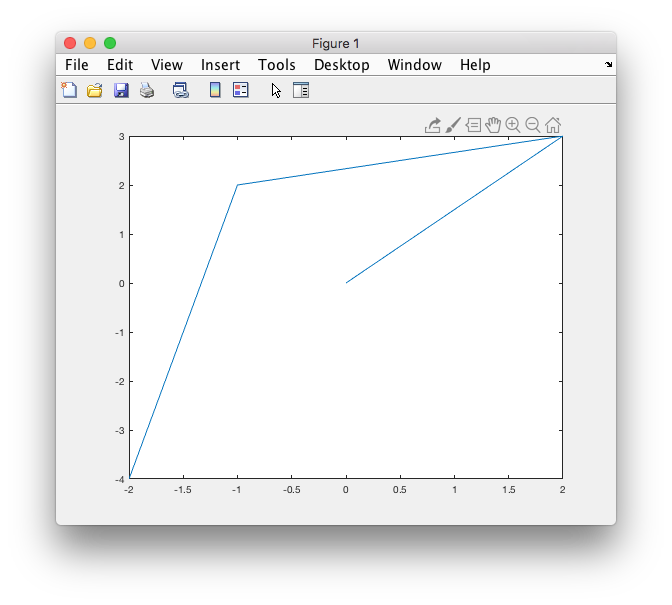
\includegraphics[width=12cm]{figura.png}
\caption{Ventana gr�fica de Matlab. representaci�n de los punto de la tabla \ref{tpuntos}}
\label{fig:ventana}
\end{figure}

La ventana gr�fica de Matlab, tiene en su parte superior una barra de herramientas y un men� desplegable con funciones espec�ficas para la manipulaci�n de los gr�ficos. Se aconseja leer la ayuda de Matlab sobre el uso de dichas herramientas.

Una de las opciones del men� desplegable, permite guardar la figura generada como un archivo gr�fico. Adem�s, es posible mediante otra de las opciones del men� copiar la figura y pegarla posteriormente en un editor de texto\footnote{Al menos es posible hacerlo as� si se trabaja en el sistema operativo Windows de Microsoft.}. Si copiamos la figura \ref{fig:ventana} y la pegamos directamente en el texto obtendr�amos un gr�fico como el de la figura, \ref{fig:plot}. A partir de ahora importaremos de esta manera todas las figuras que construyamos con Matlab.

\begin{figure}[h]
\centering
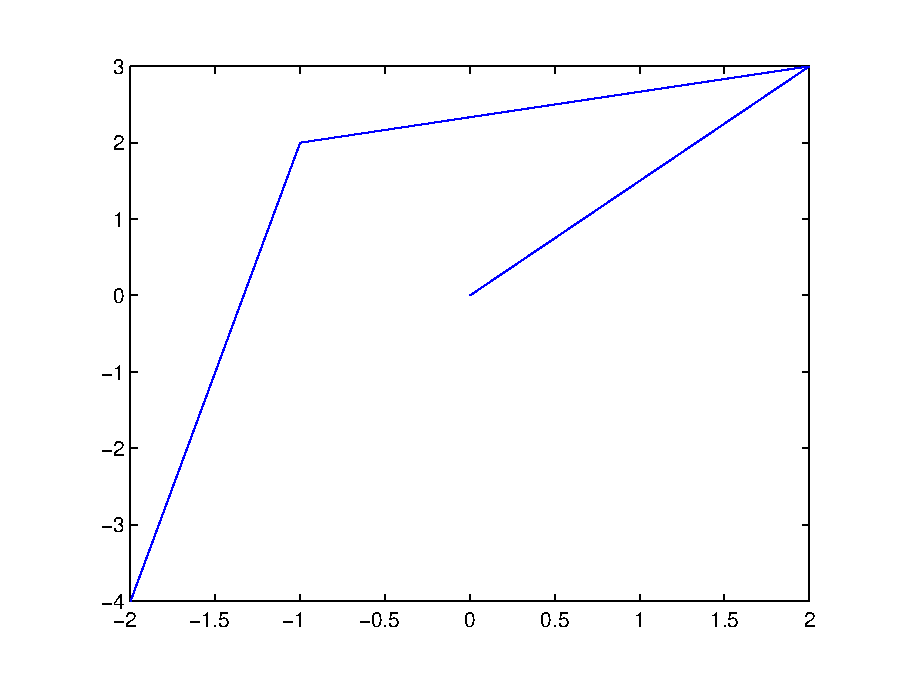
\includegraphics[width=12cm]{plot.eps}
\caption{gr�fico de los puntos de la tabla \ref{tpuntos} obtenida con el comando \texttt{plot}}
\label{fig:plot}
\end{figure}
El comando plot admite un tercer par�metro de entrada. Se trata de s�mbolos, escritos entre comillas simples, que permiten definir: 
\begin{itemize}
\item El tipo de l�nea que se emplear� en el gr�fico. por ejemplo \texttt{plot(x,y,'-.`')} une los puntos mediante una l�nea de puntos y guiones.
\item El s�mbolo que se emplear� para representar los puntos. Por ejemplo, \texttt{plot(x,y,'o')} dibuja un c�rculo en la posici�n de cada punto y no los une entre s� mediante l�neas rectas.
\item El color que se emplear� para dibujar. Por ejemplo, \texttt{plot(x,y,'r')}. Dibuja la gr�fica en color rojo.
\end{itemize}

Si no se define este tercer par�metro, \texttt{plot} dibujar� los gr�ficos, por defecto, en color azul, uniendo los puntos con l�neas continuas y no usar� ning�n s�mbolo para dibujar los puntos individuales.
 
La tabla \ref{tcolor} muestra los s�mbolos disponibles para dibujar con el comando \texttt{plot}.

\begin{table}[h]
\caption{tipos de l�nea y color del comando \texttt{plot}}
\centering
\begin{tabular}{rc|rc|rc}
Tipo de l�nea&S�mbolo&Tipo de punto& S�mbolo &Color&S�mbolo\\ 
\hline
continua&-&punto&.&azul&b\\
puntos&:&c�rculo&o&verde&g\\
puntos y guiones&-.&equis&x&rojo&r\\
guiones&--&m�s&+&cyan&c\\
&&asterisco&*&amarillo&y\\
&&diamante&d&negro&k\\
&&triangulo v�rtice abajo&v&blanco&w\\
&&triangulo v�rtice arriba&\^{}&&\\
&&triangulo v�rtice izquierda&\textless&&\\
&&triangulo v�rtice derecha&\textgreater&&\\
&&triangulo v�rtice arriba&\^{}&&\\
&&cuadrado&s&&\\
&&pent�gono&p&&\\
&&hex�gono&h&\\
\hline
\end{tabular}
\label{tcolor}
\end{table} 

Se puede combinar un s�mbolo de cada tipo en un mismo \texttt{plot}. As� por ejemplo si queremos representar los datos de la tabla \ref{tpuntos} unidos mediante una l�nea de puntos,
\begin{verbatim}
plot(x,y,':')
\end{verbatim} 

Si queremos que pinte solo los puntos sin unirlos con l�neas y en color rojo,
\begin{verbatim}
plot(x,y,'.r')
\end{verbatim}

Si queremos que pinte los puntos representados por tri�ngulos con el v�rtice hacia arriba, unidos mediante una l�nea continua y en color negro,

\begin{verbatim}
plot(x,y,'-^k')
\end{verbatim}

La figura \ref{fig:tplot} muestra los resultados de las combinaciones de s�mbolos que acabamos de describir.

\begin{figure}[h]
\centering
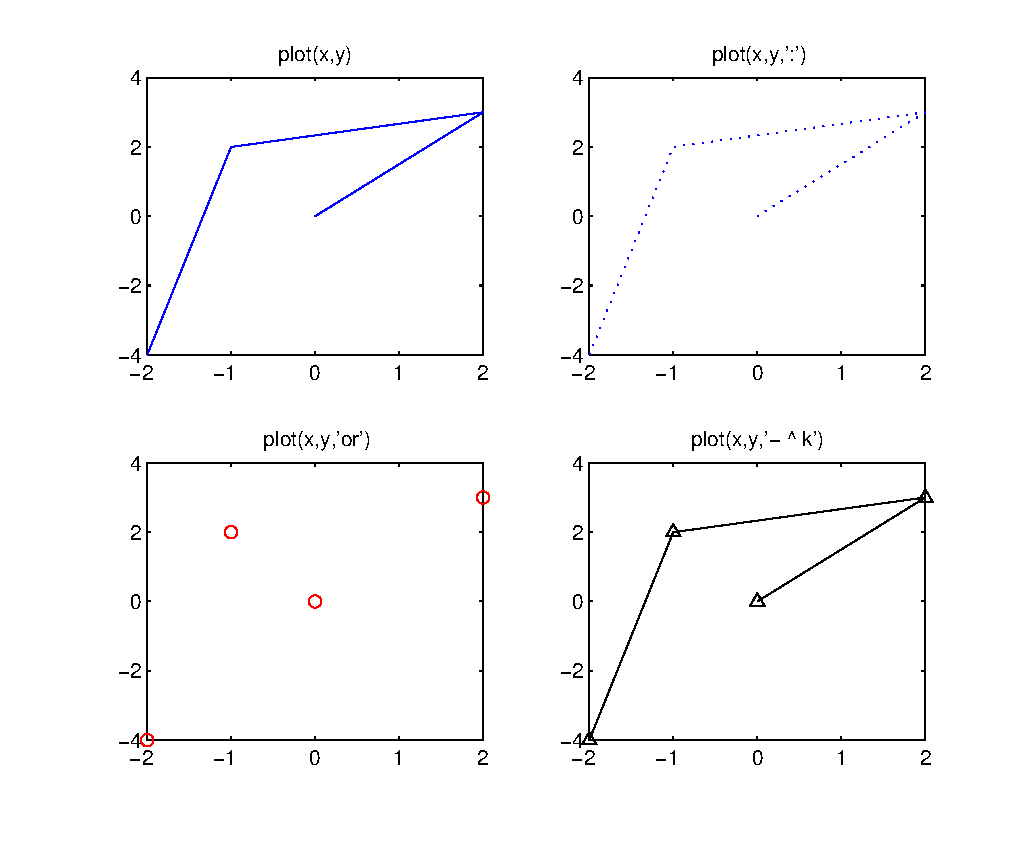
\includegraphics[width=12cm]{tiposplot.eps}
\caption{Datos de la tabla \ref{tpuntos} representados mediante distintos tipos de l�neas y colores}
\label{fig:tplot}
\end{figure}

\paragraph{Figuras.} Cada vez que escribimos en la ventana de comandos de Matlab, un comando gr�fico como por ejemplo \texttt{plot} Matlab comprueba si existe alguna figura (ventana de gr�ficos) abierta. Pueden darse entonces tres situaciones distintas. 

\begin{enumerate}
\item No hay ninguna figura abierta. Matlab crea entonces una figura nueva y representa en ella el gr�fico pedido.
\item Hay una figura abierta. Matlab emplear� dicha figura para representa el gr�fico pedido. Por defecto, Matlab borrar� cualquier gr�fico anterior que contuviese la figura.
\item Existe m�s de una figura abierta. Matlab emplear� para dibujar la llamada figura activa, que corresponde con la figura que se haya utilizado o que se haya seleccionado por �ltima vez con el rat�n.
\end{enumerate}

Es posible crear varias figuras distintas empleando directamente el comando \texttt{figure}. Cada vez que lo introduzcamos en la ventana de comandos, Matlab crear� una figura nueva asign�ndole un n�mero (figura 1, 2 ,3 etc.). Si empleamos el comando \texttt{figure}, seguido de un n�mero entre par�ntesis, \texttt{figure(25)}, Matlab crear� una nueva figura asign�ndole dicho n�mero y si ya existe la figura la convertir� en la figura activa.
El siguiente script muestra un ejemplo del uso de \texttt{figure} y \texttt{plot} combinados.

\begin{lstlisting}
% este script  (figuras.m)muestra el uso de los comandos figure y plot 
% para pintar varias funciones se aconseja copiarlo y probarlo en 
% Matlab para entender mejor c�mo funciona.

% vamos a pintar un trozo de la funci�n e^x, en concreto para el 
% intervalo x=[0,1]

% Construimos un vector de 100 puntos equiespaciados en el intervalo [0,1]

x=linspace(0,1,100);

% calculamos el valor de la funcion e^x para los puntos construidos,

y1=exp(x);

% pintamos los puntos y frente a x,

plot(x,y1) % plot ha construido una figura en Matlab, la figura 1.

% Construimos una segunda figura en Matlab
figure % se ha construido la figura 2

% construimos una tercera figura 
figure % se ha construido la figura 3


% calculamos los valores que tomar� la funci�n sin(2*pi*x) para los 
% puntos x del intervalo [0,1] que ya tenemos
y2=sin(2*pi*x);

% hacemos activa la figura 2
figure(2)
% pintamos en esta figura los puntos de la funci�n sin...

plot(x,y2)

% volvemos a hacer activa la figura 1
figure(1)
% pintamos ahora los puntos de la de la funci�n y=e^x, pero invertidos 
% x frente a y, La grafica anterior se borra y es sustituida por la nueva,
plot(y1,x)

% creamos una nueva figura asign�ndole un numero al crearla,
figure(13)

% volvemos activar la figura 3
figure(3)

% volvemos a pintar, ahora en la figura 3, la funci�n y=e^x,
plot(x,y1)

% volvemos a activar la figura 13 y pintamos en ella de nuevo la 
% funcion sin..

figure(13)
plot(x,y2)
\end{lstlisting}

Como se ha se�alado antes, cualquier comando gr�fico que se ejecute borra por defecto el contenido anterior de la figura activa. Es posible cambiar este comportamiento, empleando para ello el comando \texttt{hold}. Si en la ventana de comandos escribimos \texttt{hold on}, a partir de ese momento la ventana activa mantendr� cualquier gr�fico que contenga y a�adir� a este los nuevos gr�ficos que se creen. Este comportamiento se mantiene hasta que vuelva a escribirse en la ventana de comandos la sentencia \texttt{hold off}. El siguiente script muestra un ejemplo del uso de este comando y La figura \ref{fig:sico} el gr�fico resultante.

\begin{lstlisting}
% ejemplo de uso de hold on para representar dos funciones en el mismo
% gr�fico

% vamos a representar las funciones seno y coseno en el intervalo [-pi, pi]

% creamos un vector de 100 puntos en el intervalo,
x=[-pi:2*pi/99:pi];

% calculamos el valor de la funci�n seno sobre los puntos x
seno=sin(x);

% calculamos el valor de la funci�n coseno sobre los puntos x
coseno=cos(x);

% pintamos la funcion seno, con linea continua azul
plot(x,seno)

% le pedimos que mantenga el gr�fico creado
hold on

% pintamos encima la funci�n coseno en linea continua roja

plot(x,coseno,'r')

\end{lstlisting}


\begin{figure}[h]
\centering
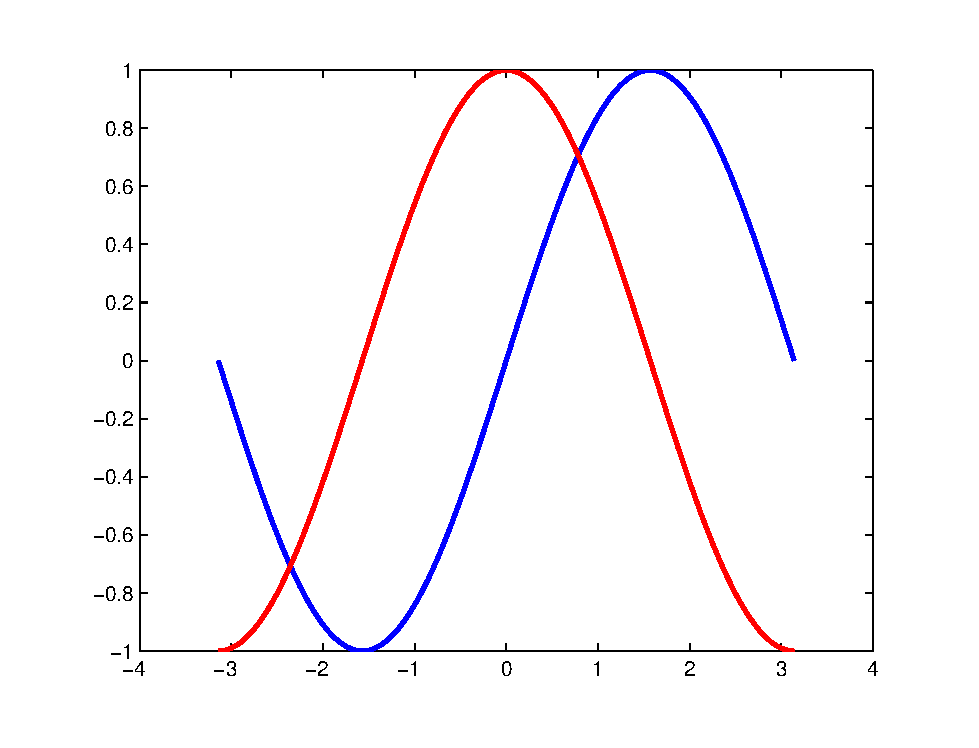
\includegraphics[width=12cm]{sico.eps}
\caption{gr�ficas de las funciones seno y coseno en el intervalo $(-\pi, \pi)$. Representadas en la misma figura, usando el comando \texttt{hold on}.}
\label{fig:sico}
\end{figure}

Es posible tambi�n incluir varios gr�ficos separados en la misma figura. 
Para ello se emplea el comando \texttt{subplot(i,j,k)}. Este comando divide la figura en un total de $i\times j$ gr�ficos y activa el situado en la posici�n $k$, las posiciones se cuentan fila a fila de arriba a abajo. El siguiente script muestra el uso del comando \texttt{subplot} La figura \ref{fig:subplot} muestra el resultado obtenido.
\begin{figure}[h]
\centering
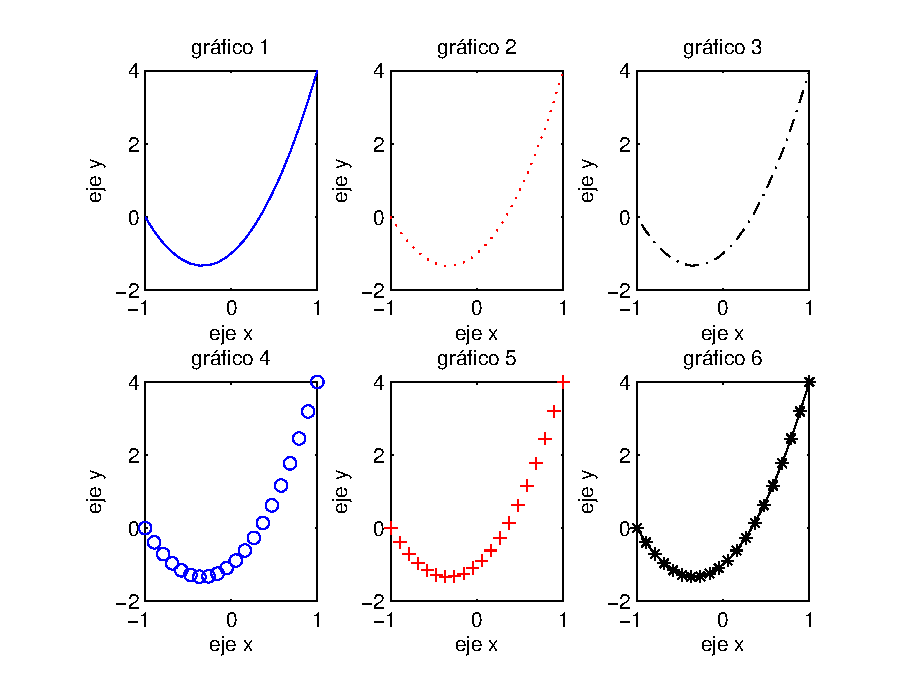
\includegraphics[width=12cm]{subplot.eps}
\caption{Ejemplo de empleo del comando subplot}
\label{fig:subplot}
\end{figure}


\begin{lstlisting}
% Este script muestra el uso del comando subplot

% vamos a crear una figura con 2X3=6 gr�ficas, se disponen en la figura 
% como si fueran los elementos de una matriz...
% usamos el comando subplot de modo que cree el primer eje de los 6
subplot(2,3,1)

% definimos un vector x de puntos equiespacios en el intervalo (-1,1)
x=linspace(-1,1,20);

% calculamos los valores de polinomio 3x^2+2^x-1
y=3*x.^2+2*x-1;

% dibujamos la funci�n en los ejes
plot(x,y)

% A�adimos r�tulos a los ejes
xlabel('eje x')
ylabel('eje y')
% A�adimos un titulo al grafico
title('gr�fico 1')

% Generamos los siguientes ejes (a la derecha del anterior)
subplot(2,3,2)
% dibujamos la misma funci�n pero ahora en linea discontinua roja
plot(x,y,':r')

% A�adimos r�tulos a los ejes
xlabel('eje x')
ylabel('eje y')
% A�adimos un titulo al grafico
title('gr�fico 2')

% Generamos los siguientes ejes (a la derecha del anterior)
subplot(2,3,3)
% dibujamos la misma funci�n pero ahora en linea de punto y raya negra
plot(x,y,'-.k')

% A�adimos r�tulos a los ejes
xlabel('eje x')
ylabel('eje y')
% A�adimos un titulo al grafico
title('gr�fico 3')

% Generamos los siguientes ejes (debajo de los primeros)
subplot(2,3,4)
% dibujamos la misma funci�n pero ahora solo con circulos azules
plot(x,y,'o')

% A�adimos r�tulos a los ejes
xlabel('eje x')
ylabel('eje y')
% A�adimos un titulo al grafico
title('gr�fico 4')

% Generamos los siguientes ejes (a la derecha del anterior)
subplot(2,3,5)
% dibujamos la misma funci�n pero ahora solo con cruce rojas
plot(x,y,'+r')

% A�adimos r�tulos a los ejes
xlabel('eje x')
ylabel('eje y')
% A�adimos un titulo al grafico
title('gr�fico 5')

% Generamos los �ltimos ejes (a la derecha del anterior)
subplot(2,3,6)
% dibujamos la misma funci�n pero ahora en linea continua y asteriscos
% negros
plot(x,y,'-*k')

% A�adimos r�tulos a los ejes
xlabel('eje x')
ylabel('eje y')
% A�adimos un titulo al grafico
title('gr�fico 6')
\end{lstlisting}


En el ejemplo, se ha hecho usos de algunos comandos para gr�ficos que permiten introducir t�tulos. Estos son: 

\texttt{title}, introduce un titulo a un gr�fico, por ejemplo,
\begin{verbatim}
title('gr�fico de temperaturas')
\end{verbatim}

\texttt{xlabel}, a�ade un r�tulo al eje x, por ejemplo,

\begin{verbatim}
xlabel('tiempo en segundos')
\end{verbatim}

\texttt{ylabel} a�ade un r�tulo al eje y , por ejemplo,
\begin{verbatim}
ylabel('distancia en metros')
\end{verbatim}

\subsection{Gr�ficos en 2D} \index{Gr�ficos! Comandos gr�ficos en 2D}
Hasta ahora, hemos visto tan solo el comando \texttt{plot}, que nos ha servido para introducir las capacidades gr�ficas en Matlab. Como hemos visto, plot permite representar gr�ficamente colecciones de datos en dos dimensiones. Hay otros muchos comandos que permiten obtener representaciones \emph{especializadas} de datos en dos dimensiones. A continuaci�n veremos algunos de los m�s destacables.
\begin{figure}[h]
\centering
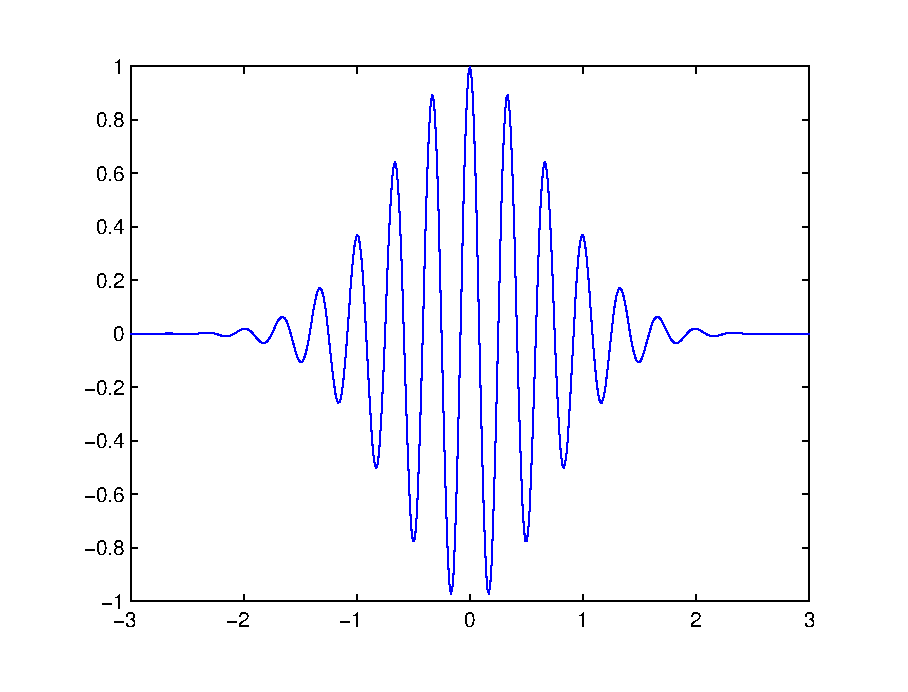
\includegraphics[width=12cm]{wave.eps}
\caption{Ejemplo de empleo del comando \texttt{fplot}}
\label{fig:wave}
\end{figure} 

\paragraph{fplot.} Permite dibujar directamente una funci�n en un intervalo de valores. El nombre de la funci�n hay que introducirlo entre comillas simples y el intervalo como un vector de dos componentes. Por ejemplo,

\begin{verbatim}
>> fplot('exp(-x.^2).*cos(6*pi*x)',[-3 3])
\end{verbatim}

dibuja la funci�n,
\begin{equation*}
f(x)=e^{-x^2}\cos(6\pi x)
\end{equation*}

en el intervalo $[-3,3]$ (figura \ref{fig:wave}).

 
\paragraph{semilogx.} El comando \texttt{semilog} representa el eje de las x en escala logar�tmica, Es decir, en lugar de representar frente a la variable $x$, se representa frente a $\log_{10}(x)$. Si dibujamos empleando este tipo de gr�fico la funci�n $y=\log_{10}(x)$ deber�amos obtener una l�near recta de pendiente unidad. La figura \ref{fig:slx} muestra el resultado, empleando para las \emph{equis} el intervalo $(0,1)$.
\begin{verbatim}
>> x=linspace(0,1,100);
>> y=log10(x);
>> semilogx(x,y)
>> grid on
\end{verbatim}

\begin{figure}[h]
\centering
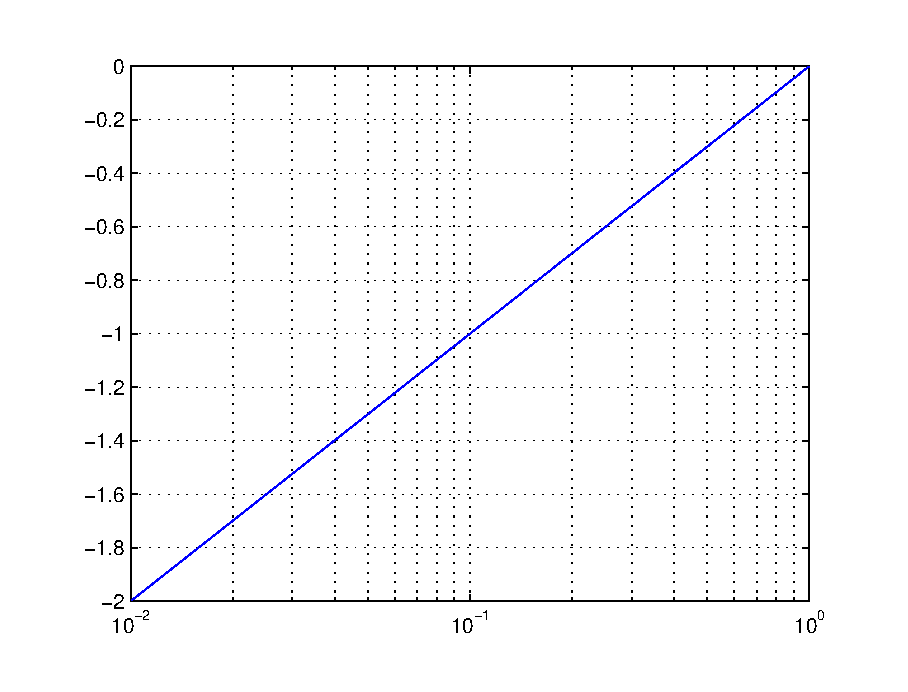
\includegraphics[width=10cm]{slx.eps}
\caption{Representaci�n de la funci�n $y=\log_{10}(x)$ empleando el comando \texttt{semilogx}}
\label{fig:slx}
\end{figure} 

Un par de observaciones sobre este ejemplo: En primer lugar las divisiones del eje x aparecen marcadas como potencias de 10. Como estamos representando empleando el logaritmo decimal de la variable x, las divisiones se corresponden con el exponente de la potencia de 10 de cada divisi�n, $\log_{10}(10^n)=n$.

En segundo lugar hemos empleado un nuevo comando gr�fico; se trata del comando \texttt{grid}. Este comando a�ade una ret�cula al gr�fico de modo que sea m�s f�cil ver los valores que toman las variables en cada punto de la gr�fica. \texttt{grid on},a�ade la ret�cula y \texttt{grid off} la retira.

\paragraph{semilogy.} An�loga al anterior, simplemente que ahora es el eje y el que se representa en escala logar�tmica. En este caso ser� si representamos la funci�n $y=10^x$ cuando obtengamos una l�nea recta,

\begin{verbatim}
>> x=linspace(0,1,100);
>> y=10.^x;
>> semilogy(x,y)
>> grid on
\end{verbatim}

\begin{figure}[h]
\centering
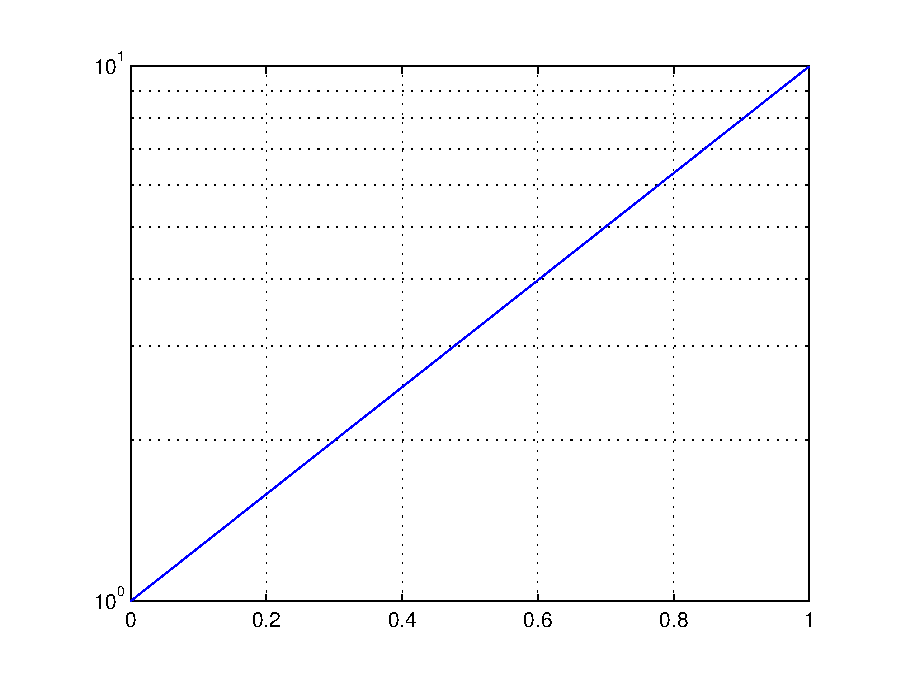
\includegraphics[width=10cm]{sly.eps}
\caption{Representaci�n de la funci�n $y=10^x$ empleando el comando \texttt{semilogy}}
\label{fig:sly}
\end{figure}

\paragraph{loglog.} An�loga a las anteriores, \texttt{loglog(x,y)} representa \texttt{y} frente a \texttt{x} empleando en ambos ejes una escala logar�tmica.


\paragraph{polar.} Representa funciones en coordenadas polares \texttt{polar(theta,r)}. La primera variable es un �ngulo en radianes y la segunda el correspondiente radio. La figura \ref{fig:esp} muestra la espiral,
\begin{equation*}
r=2\cdot\sqrt{\theta}
\end{equation*}

Para el intervalo angular $[0,8\pi]$.
 
\begin{verbatim}
>> theta=linspace(0,8*pi,100);
>> r=2*theta;
>> polar(theta,r)
>> r=sqrt(theta);
>> polar(theta,r)
\end{verbatim}

\begin{figure}[h]
\centering
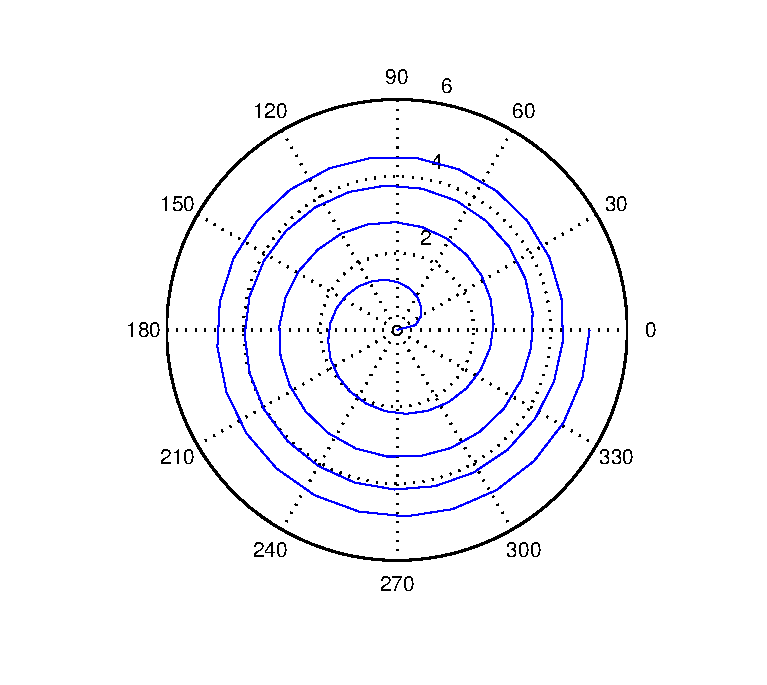
\includegraphics[width=10cm]{esp.eps}
\caption{Representaci�n de la funci�n $r=\sqrt{\theta}$ empleando el comando \texttt{polar}}
\label{fig:esp}
\end{figure}

\paragraph{stem, bar, stairs.} En los tres casos, se obtienen representaciones \emph{discretas} de un conjunto de datos. \texttt{stem} representa los datos mediante l�neas verticales que parten del eje  x y llegan hasta el valor correspondiente de y. Las l�neas van rematadas por un c�rculo. \texttt{bar} Emplea barras solidas verticales  y \texttt{stairs} realiza una representaci�n en escalera. La figura \ref{fig:sbs} muestra el resultado de dibujar, empleando estos tres tipos de gr�ficos, los datos correspondientes al n�mero de coches por cada 1000 habitantes en 2007 para cincuenta pa�ses distintos (los datos se guardaban en una matriz llamada auto\_50\_2007),

\begin{verbatim}
>> subplot(1,3,1)
>> stem(auto_50_2007)
>> subplot(1,3,2)
>> bar(auto_50_2007)
>> subplot(1,3,3)
>> stairs(auto_50_2007)
\end{verbatim}

\begin{figure}[h]
\centering
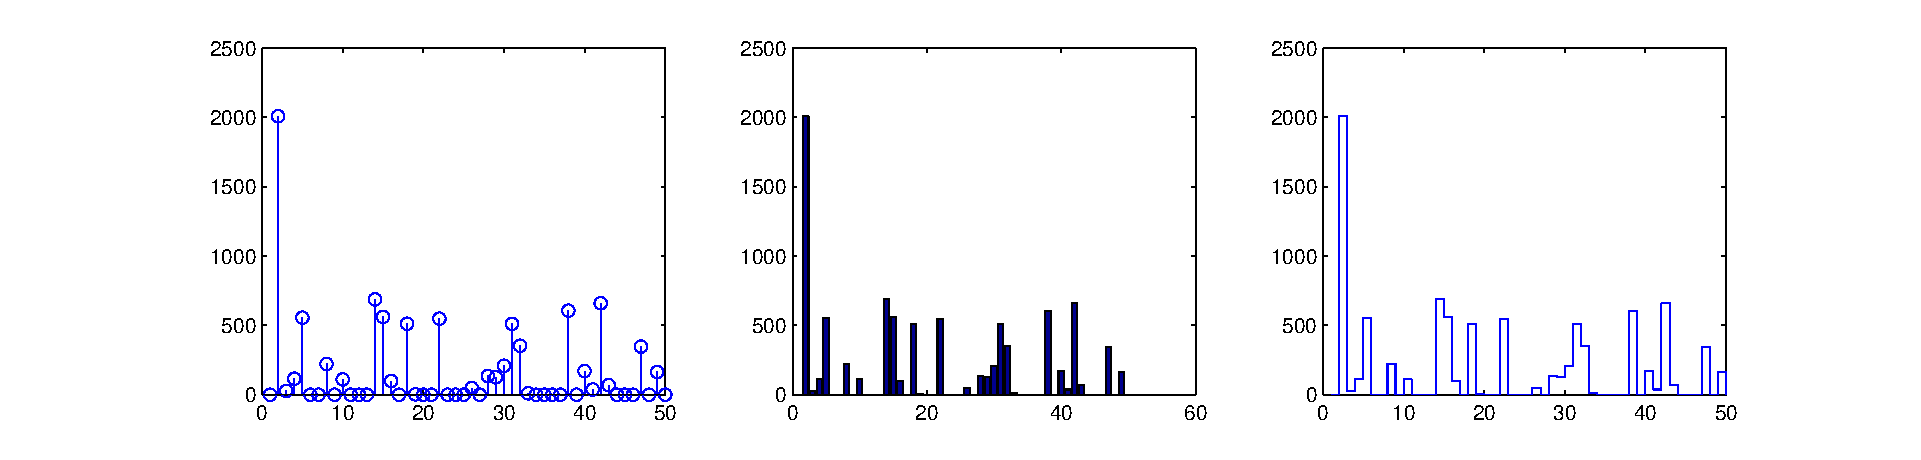
\includegraphics[width=15cm]{sbs.eps}
\caption{Comparci�n entre los comandos \texttt{stem}, \texttt{bar} y \texttt{stairs} representando la misma colecci�n de datos.}
\label{fig:sbs}
\end{figure}

\paragraph{hist.} Este comando permite dibujar el histograma de una colecci�n de datos. El histograma es una forma de representar cuantas veces se repite un dato, o m�s exactamente cuantos datos de la colecci�n caen dentro de un intervalo dado. La funci�n \texttt{hist(x,n)} admite dos par�metros de entrada, un vector de datos \texttt{x} y un valor entero \texttt{n} que representa el n�mero de intervalos en que se dividir� el rango de valores de \texttt{x}, para obtener el histograma. Si no se introduce esta segunda variable, Matlab por defecto divide el rango de los datos en 10 intervalos. Veamos un ejemplo de uso de hist, empleando los datos del ejemplo anterior relativos a n�mero de coches por cada mil habitantes. Representaremos el histograma para un total de 213 pa�ses. Para tener una idea, del rango de los dato, calculamos el valor m�nimo y m�ximo de los datos disponibles,
\begin{verbatim}
>> minimo=min(auto2007)
minimo =

     0

>> maximo=max(auto2007)

maximo =

   874
\end{verbatim}

El rango va de $0$ a $879$ autom�viles por cada mil habitantes. La figura \ref{fig:hist} muestra los histogramas obtenidos sin indicar el n�mero de intervalos, ---por lo que se tomar�n 10---, tomando 5 intervalos y tomando 20.

\begin{verbatim}
>> subplot(1,3,1)
>> hist(auto2007)
>> subplot(1,3,2)
>> hist(auto2007,5)
>> subplot(1,3,3)
>> hist(auto2007,20)
>> subplot(1,3,1)
>> title('10 intervalos')
>> subplot(1,3,2)
>> title('5 intervalos')
>> subplot(1,3,3)
>> title('20 intervalos')
\end{verbatim}

\begin{figure}[h]
\centering
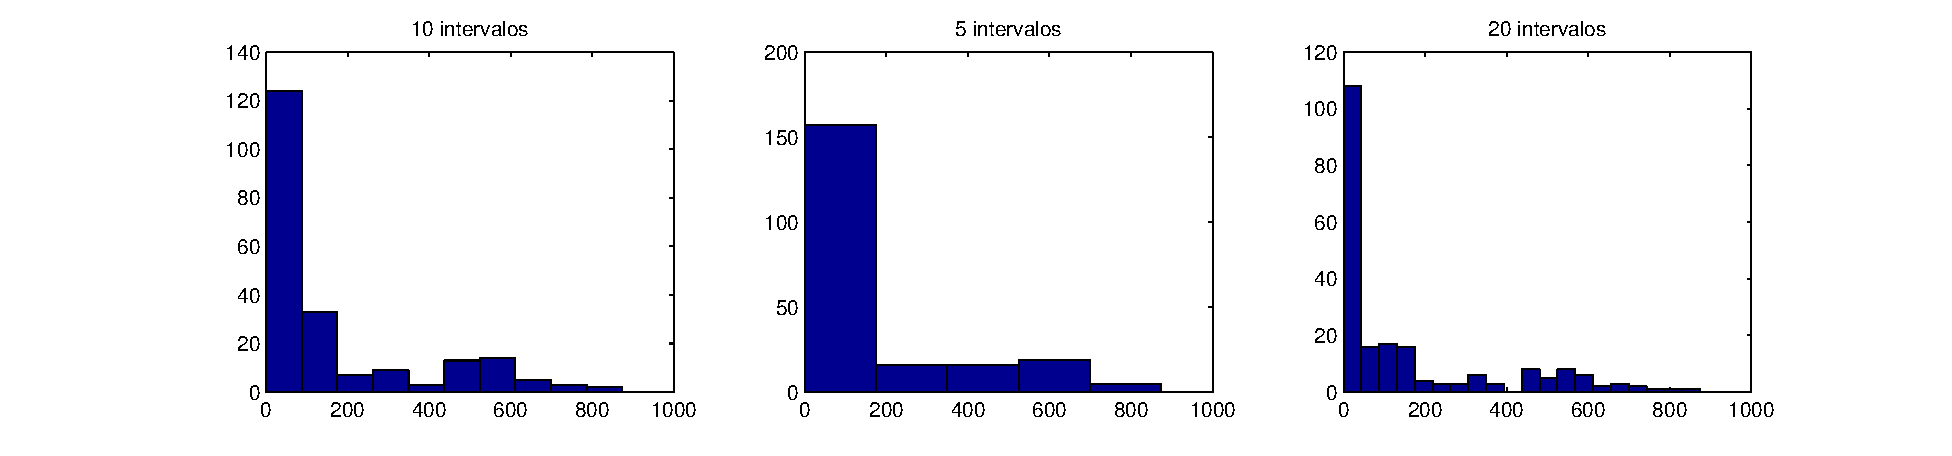
\includegraphics[width=15cm]{hist.eps}
\caption{histogramas del n�mero de autom�viles por cada 1000 habitantes para 213 pa�ses}
\label{fig:hist}
\end{figure}

La interpretaci�n del los histogramas depende l�gicamente del n�mero de intervalos. En el caso de 10 intervalos, estos dividen los datos en grupos de aproximadamente 100 coches. Si observamos el histograma resultante, podemos concluir que hay unos 120 pa�ses en los que hay entre 0 y 100 autom�viles por cada 1000 habitante, unos 30 pa�ses en los que hay entre 100 y 200 autom�viles por cada 1000 habitante, etc. Si miramos el siguiente histograma, en el que se han empleado tan solo 5 intervalos, los grupos son ahora de aproximadamente 200 coches. La primera barra de este segundo histograma establece que hay unos 150 pa�ses en los que hay entre 0 y 200 coches por cada 1000 habitantes. Resultado que corresponde a la suma de los de dos primeros intervalos del histograma anterior. Para el tercer histograma los intervalos son ahora de 50 autom�viles, lo que permite observar m�s en detalle que en los histogramas anteriores la distribuci�n de veh�culos: 110 pa�ses tienen menos de 50 autom�viles por cada 1000 habitantes.

\paragraph{plotyy.} Este comando permite representar dos gr�ficas en la misma figura de modo que comparten el mismo eje x y cada una tiene su propio eje y. La figura \ref{fig:plotyy} muestra el resultado del siguiente ejemplo,

\begin{verbatim}
>> x1=linspace(0,10,100);
>> x2=linspace(0,12,50);
>> y1=x1.^2;
>> y2=x2.^(2/3);
>> plotyy(x1,y1,x2,y2)
>> grid on
\end{verbatim}

\begin{figure}[h]
\centering
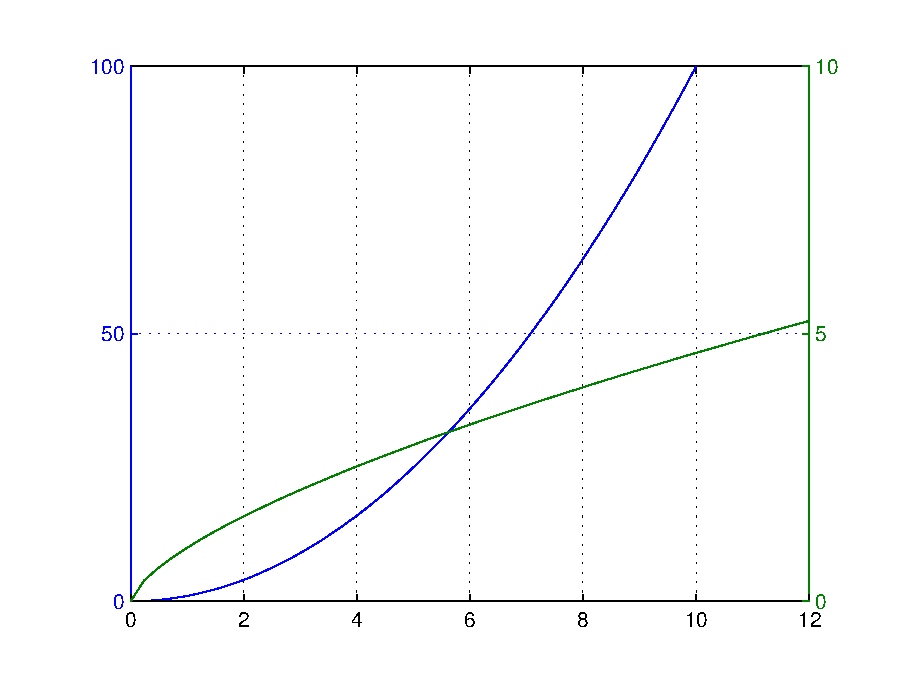
\includegraphics[width=10cm]{plotyy.eps}
\caption{Ejemplo de uso de la funci�n \texttt{plotyy}}
\label{fig:plotyy}
\end{figure}

\paragraph{quiver.} Esta funci�n de Matlab permite dibujar vectores en el plano. En realidad est� pensada para dibujar campos vectoriales, con lo que hay que manejarla con cierto cuidado. En primera aproximaci�n diremos que \texttt{quiver} necesita 5 variables de entrada: la coordenada $x$ del origen del vector, la coordenada $y$ del origen del vector, la componente $x$ del vector y la componente $y$ del vector, por �ltimo, un factor de escala al que daremos el valor $0$ para que dibuje los vectores a su tama�o real, sin modificar su escala. Por ejemplo si queremos dibujar el vector $\vec{v}=(1,2)$ situado en el origen de coordenadas,
\begin{verbatim}
quiver(0,0,1,2,0)
\end{verbatim}

Si queremos representar el mismo vector pero situado en el punto $(3,-1)$,
\begin{verbatim}
>>quiver(3,-1,1,2,0)
\end{verbatim}

Podemos dibujar un conjunto de vectores con quiver, para ello empleamos como variables de entradas vectores, en lugar de escalares; un vector que contenga las posiciones $x$ del los or�genes, un segundo vector que contenga la posiciones $y$ de los or�genes, un tercer vector que contenga las componentes $x$ de los vectores y un cuarto que contenga las componentes $y$, por �ltimo a�adir�amos el par�metro de escala $0$, que sigue siendo un escalar.

Por tanto, si queremos dibujar a la vez los dos vectores de los ejemplos anteriores,

\begin{verbatim}
>>quiver([0 3],[0 -1],[1 1],[2 2],0)
\end{verbatim}

La figura \ref{fig:quiver} muestra los resultados del ejemplo que acabamos de ver,

\begin{figure}[h]
\centering
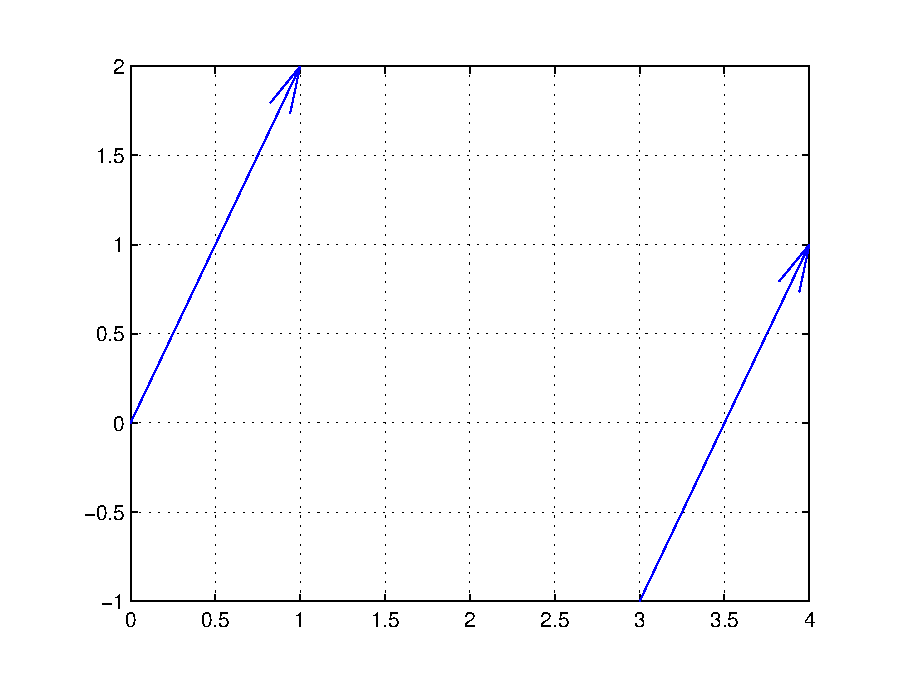
\includegraphics[width=10cm]{quiver.eps}
\caption{Ejemplo de uso de la funci�n \texttt{quiver}}
\label{fig:quiver}
\end{figure}

\paragraph{errorbar.} Permite a�adir barras de  error a un gr�fico de puntos experimentales. Supongamos que tenemos la siguiente tabla (\ref{vel}) de resultados de la medida de la velocidad de un m�vil frente al tiempo,


\begin{table}[h]
\caption{Resultados experimentales de la medida de la velocidad de un m�vil}
\centering
\begin{tabular}{ccc}
\hline
\hline
tiempo &velocidad& incertidumbre\\ 
$t$ (s)&$v$ (m/s)& $\pm \Delta v$ (m/s)\\
\hline
0&0&0\\
1&2.8&0.8\\
2&4.0&0.8\\
3&4.3&0.9\\
4&4.2&0.9\\
5&4.8&1.0\\
6&6.3&1.0\\
7&7.9&1.0\\
8&8.9&1.1\\
9&9.0&1.1\\
10&8.7&1.1\\
\hline
\hline
\end{tabular}
\label{vel}
\end{table} 

La primera columna representa el instante de tiempo en que se tom� la medida, la segunda columna representa el valor medido de la velocidad y la tercera columna la incertidumbre de cada medida de velocidad.

podemos emplear el comando \texttt(errorbar) para representar la velocidad frente al tiempo, a�adiendo una barra de error en cada medida que represente la incertidumbre,

\begin{verbatim}
>> vel=[0 2.8 4.0 4.3 4.2 4.8 6.3 7.9 8.9 9.0 8.7]
vel =

  Columns 1 through 7

         0    2.8000    4.0000    4.3000    4.2000    4.8000    6.3000

  Columns 8 through 11

    7.9000    8.9000    9.0000    8.7000

>> inc=[0 0.8 0.8 0.9 0.9 1.0 1.0 1.0 1.1 1.1 1.1]
inc =

  Columns 1 through 7

         0    0.8000    0.8000    0.9000    0.9000    1.0000    1.0000

  Columns 8 through 11

    1.0000    1.1000    1.1000    1.1000

>> t=0:10
t =

     0     1     2     3     4     5     6     7     8     9    10

>> errorbar(t,vel,inc)
>> xlabel('tiempo s')
>> ylabel('velocidad m/s')
\end{verbatim}

EL resultado se muestra en la figura \ref{fig:error}. Es interesante hacer notar que la longitud total de cada barra de error es el doble del valor de la incertidumbre correspondiente al punto. Por ejemplo para $t=1s, v+\Delta v=2.8\pm 0.8 m/s$ la longitud de la barra de error es $2\cdot \Delta v=1.6 m/s$). El comando \texttt{errobar}, puede tambi�n emplearse para representar incertidumbres asim�tricas. Para ello  es preciso suministrar dos vectores uno \texttt{U} para dibujar la parte superior de la barra de error y otro \texttt{L} para dibujar la parte inferior; \texttt{errorbar(x,y,L,U)}. 

\begin{figure}[h]
\centering
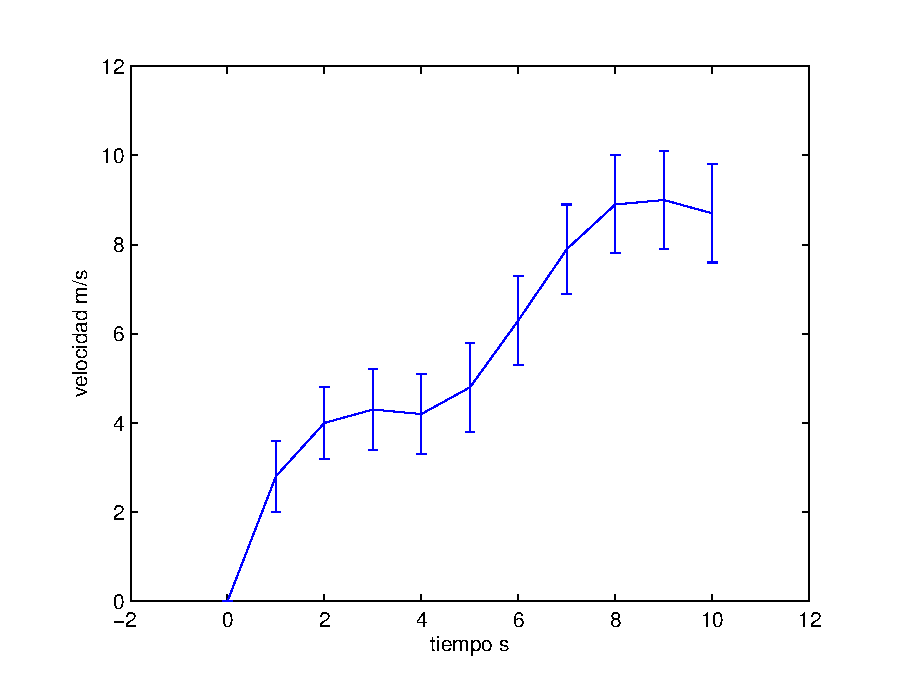
\includegraphics[width=11cm]{error.eps}
\caption{Datos de la tabla \ref{vel} representados empleando el comando \texttt{errorbar}}
\label{fig:error}
\end{figure}

\subsection{Gr�ficos en 3D.} \index{Gr�ficos! Comandos gr�ficos en 3D}En tres dimensiones es posible representar dos tipos de gr�ficos: puntos y curvas, an�logos a los representados en dos dimensiones y adem�s superficies en el espacio.

\paragraph{plot3.} Para dibujar l�neas y puntos Matlab emplea los mismos comandos que hemos descrito para dos dimensiones, a�adiendo al nombre de comando la terminaci�n \texttt{3} para indicar que se trata de un gr�fico en tres dimensiones. As� por ejemplo el comando \texttt{plot3} nos permite dibujar puntos y curvas en el espacio. El manejo es id�ntico al de \texttt{plot}, simplemente que ahora es preciso a�adir un vector que contenga los datos de la tercera coordenada, z. 

Por ejemplo, podemos representar la curva,
\begin{align*}
y&=\sin(2\pi x)\\
z&=\cos(2\pi x)
\end{align*}

Para ello, seleccionamos un intervalo de valores para $x \in (0,2)$, y calculamos los correspondientes valores de $y$ y $z$,

\begin{verbatim}
>> x=linspace(0,2,100);
>> y=sin(2*pi*x);
>> z=cos(2*pi*x);
\end{verbatim}

Podemos ahora representar la gr�fica de nuestra funci�n empleando el comando \texttt{plot3},
\begin{verbatim}
>> plot3(x,y,z)
>> grid on
>> xlabel('x')
>> ylabel('y')
>> zlabel('z')
\end{verbatim}

Hemos a�adido los comandos \texttt{grid on}  para obtener una trama en 3D que permita ver mejor el resultado. La figura \ref{fig:muelle1} muestra la figura de Matlab obtenida, donde se ha se�alado adem�s un bot�n que permite rotar la figura, cambiando la vista. Para ellos, una vez pulsado el bot�n, basta con arrastrar el rat�n sobre la figura manteniedo pulsado el boton izquierdo.  La figura \ref{fig:muelle2}, muestra la misma gr�fica en 3D, pero ahora vista de frente (como si nos situ�ramos en el eje x). La figura \ref{fig:muelle3}, nos muestra la grafica vista desde arriba (desde el eje z), por �ltimo, la figura \ref{fig:muelle4} muestra una vista lateral de la gr�fica (tomada desde el eje y).

Es posible rotar la figura par a obtener una vista concreta mediante el comando \texttt{view(Az, El)}. Este comando admite dos par�metros; \texttt{Az}, representa el azimuth o �ngulo de rotaci�n horizontal, \texttt{El}, representa el �ngulo de elevaci�n. Ambos �ngulos se introducen en grados. As�, por ejemplo las vistas representadas en las figuras anteriores, se pueden obtener como,
\begin{verbatim}
>> view(90,0)
>> view(0,90)
>> view(0,0)
\end{verbatim}

\begin{figure}[h]
\centering
\subfigure[ventana gr�fica \label{fig:muelle1}]{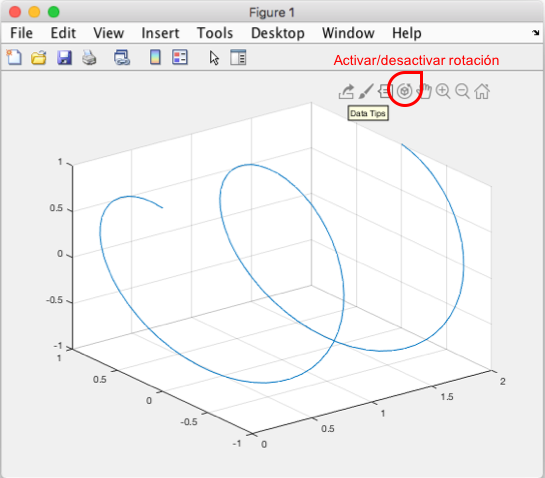
\includegraphics[width=6cm]{muelle1.png}} \qquad 
\subfigure[vista frontal (eje x) \label{fig:muelle2}]{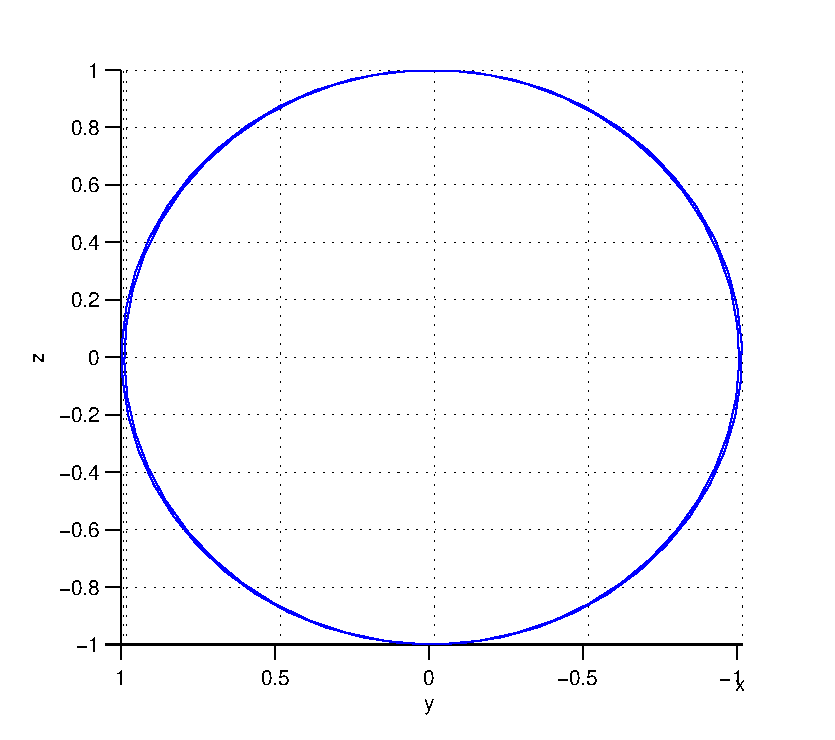
\includegraphics[width=6cm]{muelle2.eps}}\\
\subfigure[vista desde arriba (eje z) \label{fig:muelle3}]{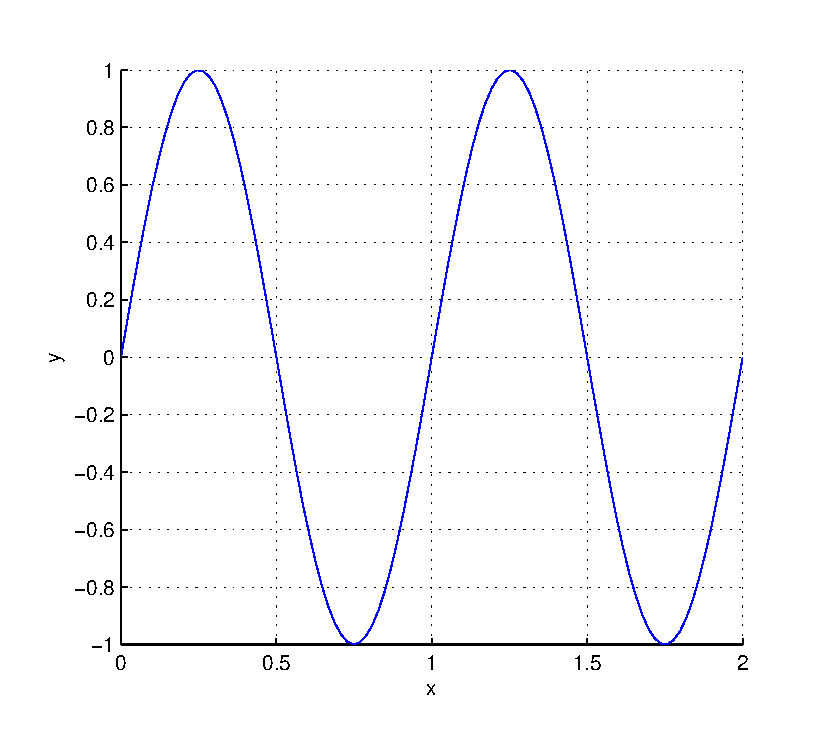
\includegraphics[width=6cm]{muelle3.eps}}\qquad
\subfigure[vista lateral (eje y)l \label{fig:muelle4}]{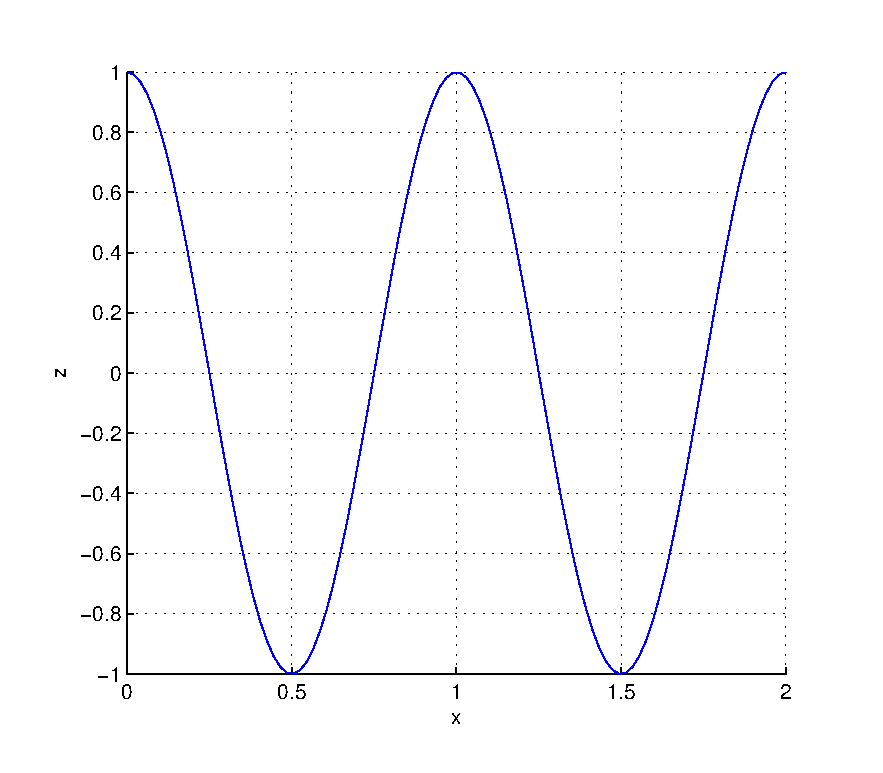
\includegraphics[width=6cm]{muelle4.eps}}\\
\caption{Gr�fico en 3D y rotaciones. }
\end{figure}

\paragraph{bar3, stem3, hist3, quiver3.} Existen versiones 3D de los comandos \texttt{bar}, \texttt{stem}, \texttt{hist} y \texttt{quiver}. Su funcionamiento es similar ---aunque no siempre igual--- al de la versi�n 2D que vimos en la secci�n anterior. En algunos casos necesitan tres variables de entrada, correspondientes a las componentes (x,y,z) de los datos que se quiere representar, y en otros necesitan que los datos de entrada se le suministren en forma de matriz. Para conocer en detalle su funcinamiento, lo ideal es acudir a la ayuda de Matlab.


\paragraph{Superficies.}Para trazar superficies en el espacio, Matlab necesita en primer lugar que se defina una ret�cula en el plano $(x,y)$ que sirve de base sobre la que calcular los puntos z sobre los que se alzar� la superficie.

Para definir dicha ret�cula Matlab emplea dos matrices. una de ellas $X_m$ contiene las coordenadas $x$ de los nodos de la ret�cula y la otra $Y_m$ las coordenadas $y$. Los elementos que ocupan la misma posici�n en ambas matrices, representan ---juntos--- un punto en el plano.
Matlab emplea dichas matrices como matrices de \emph{adyacencia}. Cada nodo, $(x_m(i,j),y_m(i,j)$, aparecer� en la gr�fica conectado por una arista a cada uno de sus cuatros puntos vecinos, $(x_m(i-1,j),y_m(i-1,j)$, $(x_m(i,j-1),y_m(i,j-1)$, $(x_m(i+1,j),y_m(i+1,j)$, $(x_m(i,j+1),y_m(i,j+1)$.
Supongamos que empleamos las siguientes matrices, $X_m$ y $Y_m$ para definir una ret�cula sobre la que dibujar una superficie,

\begin{align*}
X_m=\begin{pmatrix}
0&1&2&3\\ 
0&1&2&3\\
0&1&2&3\\
0&1&2&3
\end{pmatrix},& Y_m\begin{pmatrix}
0&0&0&0\\
1&1&1&1\\
2&2&2&2\\
3&3&3&3
\end{pmatrix}\xrightarrow[nodos]{posiciones}\begin{matrix}
(0,0)&-&(1,0)&-&(2,0)&-&(3,0)\\
\vert&&\vert&&\vert&&\vert\\ 
(0,1)&-&(1,1)&-&(2,1)&-&(3,1)\\
\vert&&\vert&&\vert&&\vert\\
(0,2)&-&(1,2)&-&(2,2)&-&(3,2)\\
\vert&&\vert&&\vert&&\vert\\
(0,3)&-&(1,3)&-&(2,3)&-&(3,3)
\end{matrix}
\end{align*}

La ret�cula definida por Matlab, a partir de dichas matrices tendr�a el aspecto que se muestra en la figura \ref{fig:mesh}. 

\begin{figure}[h]
\centering
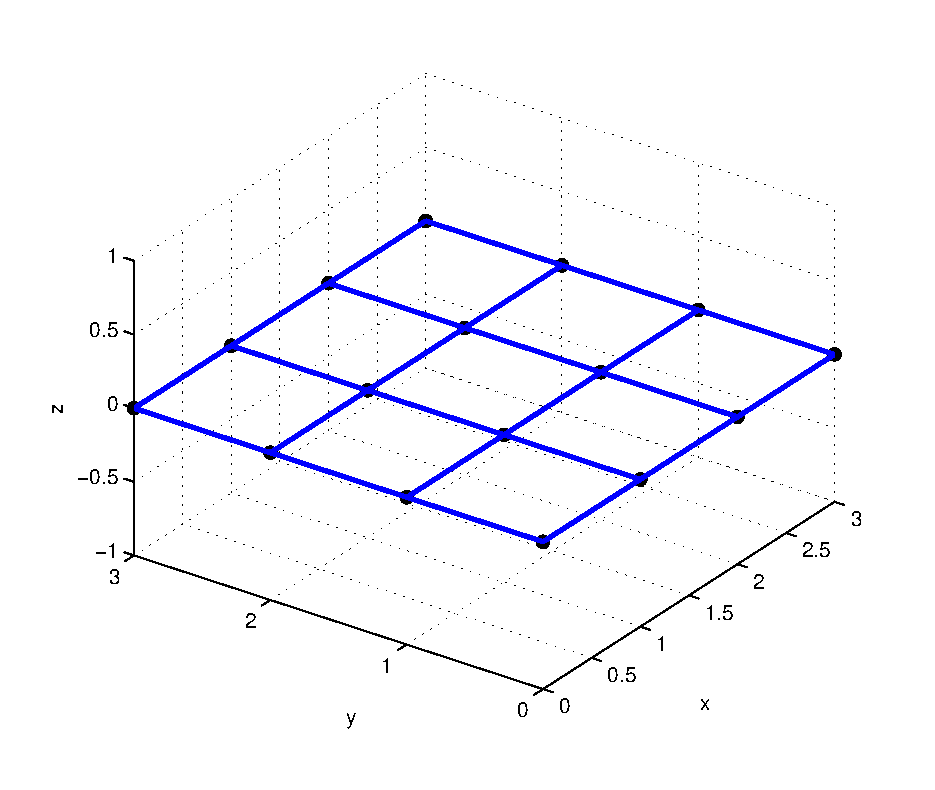
\includegraphics[width=11cm]{mesh.eps}
\caption{Ret�cula para representar superficies. Los puntos negros son los nodos definidos por las matrices $X_m$ e $Y_m$.}
\label{fig:mesh}
\end{figure}

Si nos fijamos en los ejes de la figura es f�cil obtener las coordenadas de los nodos y comprobar como, est�n unidos entre s� por aristas los que ocupan posiciones adyacentes en las matrices $X_m$ e $Y_m$.

Para construir una superficie sobre la ret�cula, lo �nico que hace falta es definir una altura (z), para cada punto de la ret�cula. Para ello, Matlab emplea una matriz, del mismo tama�o que $X_m$ y $Y_m$. As� por ejemplo, si definimos,

\begin{equation*}
Z_m=\begin{pmatrix}
0&0&0&\\ 
0&1&2&0\\
0&3&4&0\\
0&0&0&0
\end{pmatrix}
\end{equation*}

Cada elemento de la matriz $Z_m$ representa la altura del nodo correspondiente a las posiciones marcadas por las matrices $X_m$ e $Y_m$, tal y como se muestra en la figure \ref{fig:mesh1}.

\begin{figure}[h]
\centering
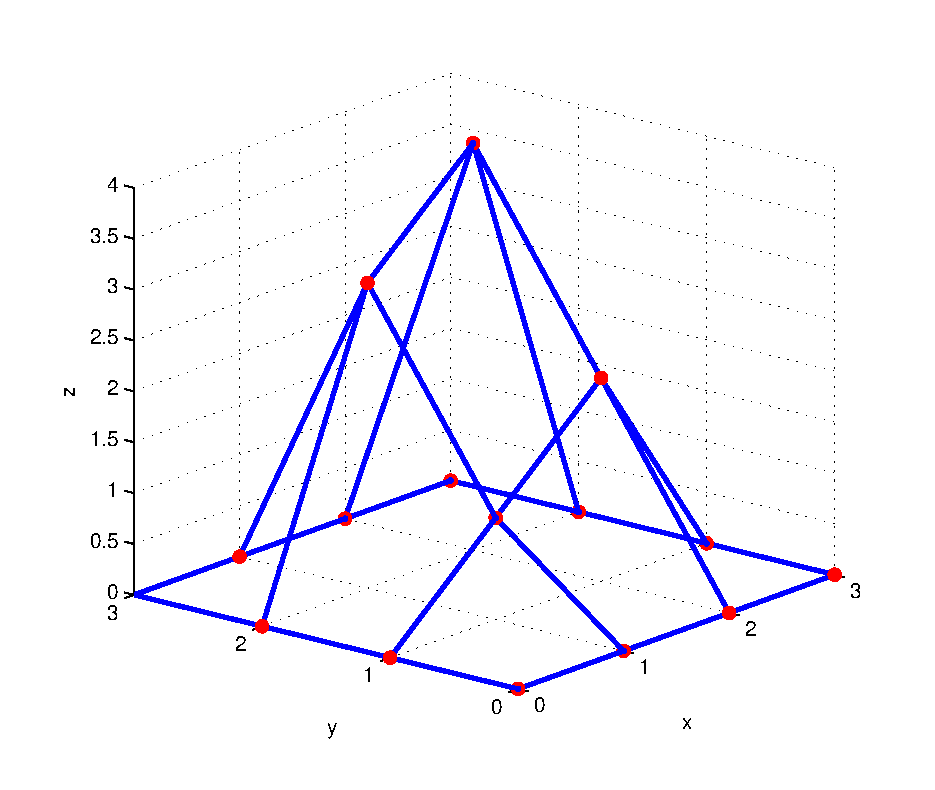
\includegraphics[width=11cm]{mesh1.eps}
\caption{Superficie elemental obtenida elevando los cuatros puntos centrales de la figura \ref{fig:mesh}.}
\label{fig:mesh1}
\end{figure}

La estructura de las matrices $X_m$ e $Y_m$ de los ejemplo anteriores, es la t�pica de las matrices de adyacencia de una ret�cula cuadrada; la matriz  $X_m$ tiene la filas repetidas y la matriz $Y_m$ tiene repetidas la columnas. En el ejemplo las matrices son cuadradas y definen una ret�cula de $4\times 4$ nodos. En general, podemos definir una ret�cula rectangular de $m\times n$ nodos. En este caso las matrices empleadas para definir la ret�cula tendr�an dimensi�n $m\times n$.

Para dibujar en Matlab superficies podemos en primer lugar definir la ret�cula a partir de dos vectores de coordenadas empleando el comando \texttt{meshgrid}. En el ejemplo que acabamos de ver, hemos empleado una ret�cula que cubre el intervalo, $x\in[0,3]$ e $y\in[0,3]$. para definirlo creamos los vectores,

\begin{verbatim}
>> x=0:3
x =

     0     1     2     3

>> y=0:3
y =

     0     1     2     3
\end{verbatim}

A continuaci�n empleamos el comando \texttt{meshgrid} para construir las dos matrices de adyacencia. Matlab se encargar� de repetir las filas y columnas necesarias,

\begin{verbatim}
>> [Xm,Ym]=meshgrid(x,y)
Xm =

     0     1     2     3
     0     1     2     3
     0     1     2     3
     0     1     2     3


Ym =

     0     0     0     0
     1     1     1     1
     2     2     2     2
     3     3     3     3

\end{verbatim}

Una vez construidas las matrices de adyacencia, solo necesitamos una matriz de valores para $Z_m$. Si definimos por ejemplo,
\begin{verbatim}
>> Zm=zeros(size(Xm))

Zm =

     0     0     0     0
     0     0     0     0
     0     0     0     0
     0     0     0     0
\end{verbatim}

Podr�amos representar la ret�cula plana de la figura \ref{fig:mesh}, empleando por ejemplo el comando \texttt{mesh(Xm, Ym, Zm)}.

\paragraph{mesh y surf.} Una vez que hemos visto como construir una ret�cula rectangular sobre la que construir una superficie, veamos como dibujarla con un ejemplo. Supongamos que queremos dibujar la superficie,
\begin{equation*}
z=x^3+y^2
\end{equation*}

En la regi�n del plano, $x\in[-1.5,1.5]$, $y\in[-2,2]$. 

Igual que en el ejemplo inicial, lo primero que debemos hacer es construirnos una matrices de adyacencia que definan una ret�cula en la regi�n de inter�s,
\begin{verbatim}
>> x=linspace(-1.5,1.5,25);
>> y=linspace(-2,2,50);
>> [Xm,Ym]=meshgrid(x,y);
\end{verbatim}

Es interesante notar que la regi�n de inter�s no es cuadrada y que las matrices de adyacencia tampoco los son ($50\times 25$). Adem�s los puntos no est�n espaciados igual en los dos ejes.

A continuaci�n obtenemos la matriz de coordenadas z, aplicando la funci�n a los puntos de la ret�cula,

\begin{verbatim}
>> Zm=Xm.^3+Ym.^2;
\end{verbatim}

\begin{figure}[h]
\centering
\subfigure[Funci�n $z=x^3+y^2$ representada con \texttt{mesh}\label{fig:msh}]{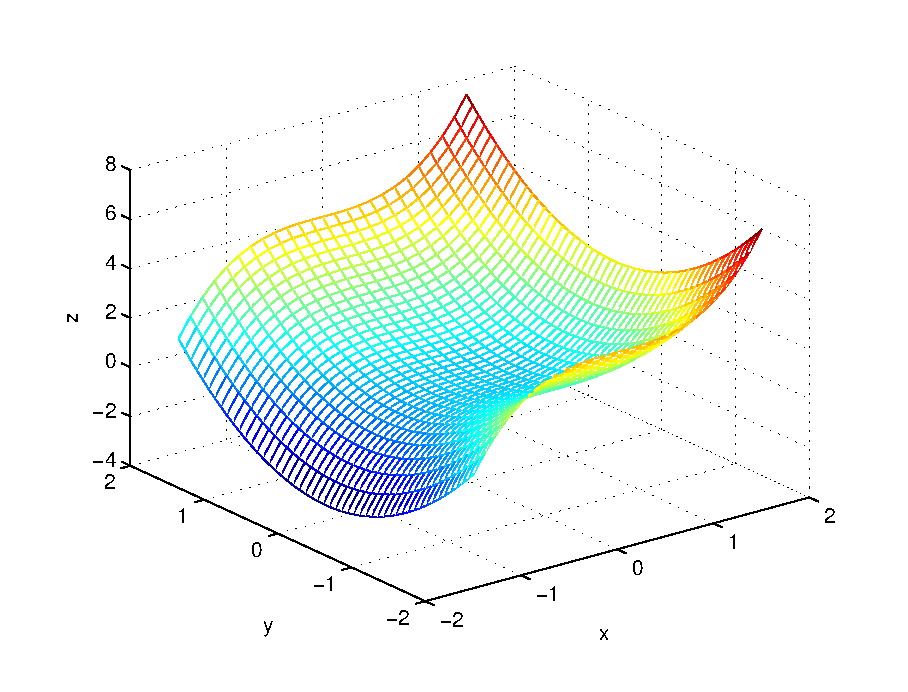
\includegraphics[width=8cm]{pa23.eps}} %\qquad 
\subfigure[Funci�n $z=x^3+y^2$ representada con \texttt{surf} \label{fig:sur}]{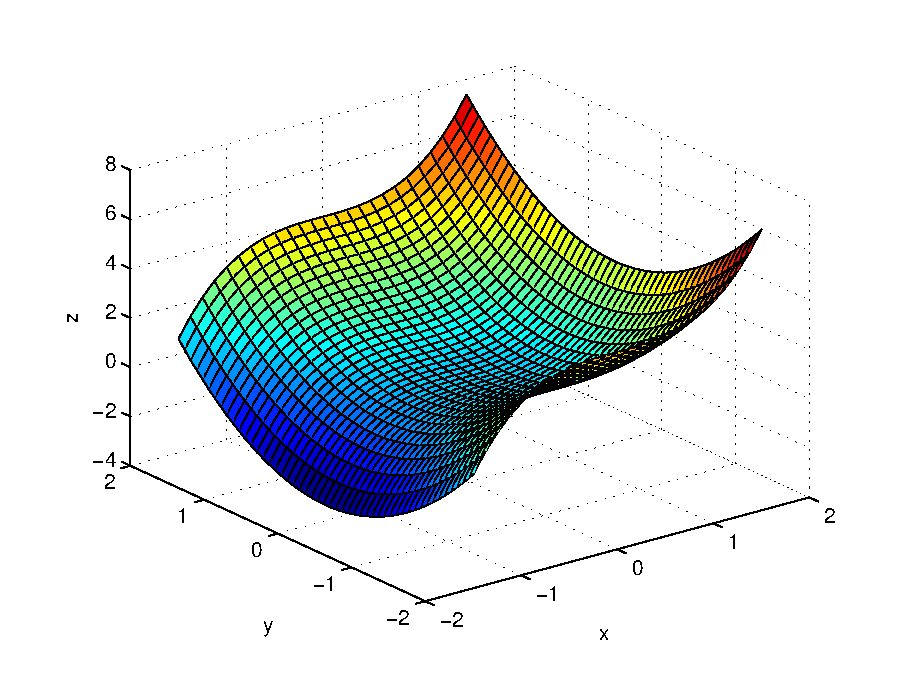
\includegraphics[width=8cm]{surf.eps}}\\
\caption{Comparaci�n entre \texttt{mesh} y \texttt{surf}}
\end{figure}

Para representar la superficie podemos emplear el comando \texttt{mesh}. 
\begin{verbatim}
>> mesh(Xm,Ym,Zm)
\end{verbatim}

Este comando admite como variables de entrada las dos matrices de adyacencia empleadas para definir la ret�cula y la matriz $Z_m$ que contiene los valores calculados para la  variable z, en todos los puntos de la ret�cula. \texttt{mesh} traza la superficie en forma reticular, es decir, nos dibuja una malla en el espacio. El color de la malla depende del valor que toma la coordenada z. Podemos tambi�n representar la superficie haciendo uso del comando \texttt{surf}, empleando las mismas variables de entrada que en el caso de \texttt{mesh}. 
\begin{verbatim}
>> surf(Xm,Ym,Zm)
\end{verbatim}

La diferencia est� en que ahora la superficie muestra las caras definidas por la malla de colores, seg�n el valor que toma la variable $z$. la figura \ref{fig:msh} muestra el resultado de nuestro ejemplo empleando \texttt{mesh} y la figura \ref{fig:sur} muestra el resultado empleando \texttt{surf}.



Para figuras que presentan simetr�a radial, puede ser m�s conveniente, definir las ret�culas en coordenadas polares. as� por ejemplo,

\begin{verbatim}
>> r=0:2/20:2;
>> theta=0:2*pi/36:2*pi;
>> [rm,them]=meshgrid(r,theta);
\end{verbatim}

Hemos cosntruido una ret�cula en las variables $r$ y $\theta$, si ahora definimos las matrices de adyacencia como las proyecciones sobre los ejes $x$ e $y$,

\begin{verbatim}
>> xm=rm.*cos(them);
>> ym=rm.*sin(them); 
\end{verbatim}

Obtenemos una ret�cula con simetr�a radial, centrada en el origen de coordenadas. Como la que se muestra en la figura, \ref{fig:retcir}.

\begin{figure}[h]
\centering
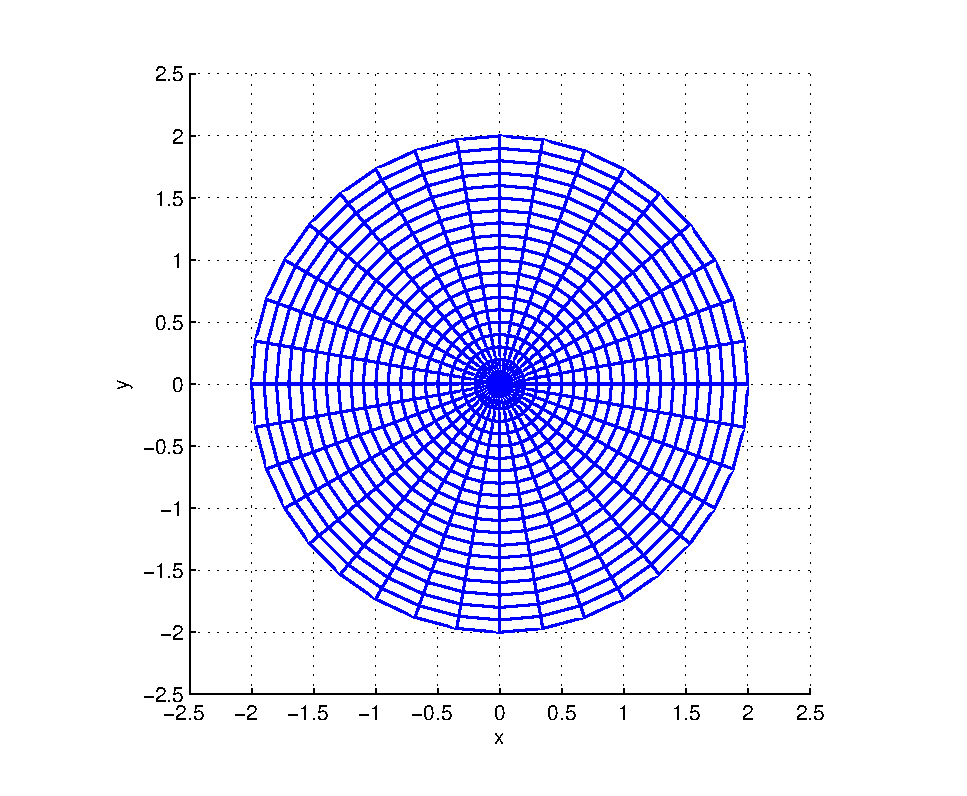
\includegraphics[width=12cm]{retcirc.eps}
\caption{ret�cula con simetr�a circular}
\label{fig:retcir}
\end{figure}

La ret�cula resulta muy adecuada para dibujar por ejemplo un cono (figura \ref{fig:cono}),

\begin{verbatim}
>> zm=2-sqrt(xm.^2+ym.^2);
>> mesh(xm,ym,zm)
\end{verbatim}

\begin{figure}[h]
\centering
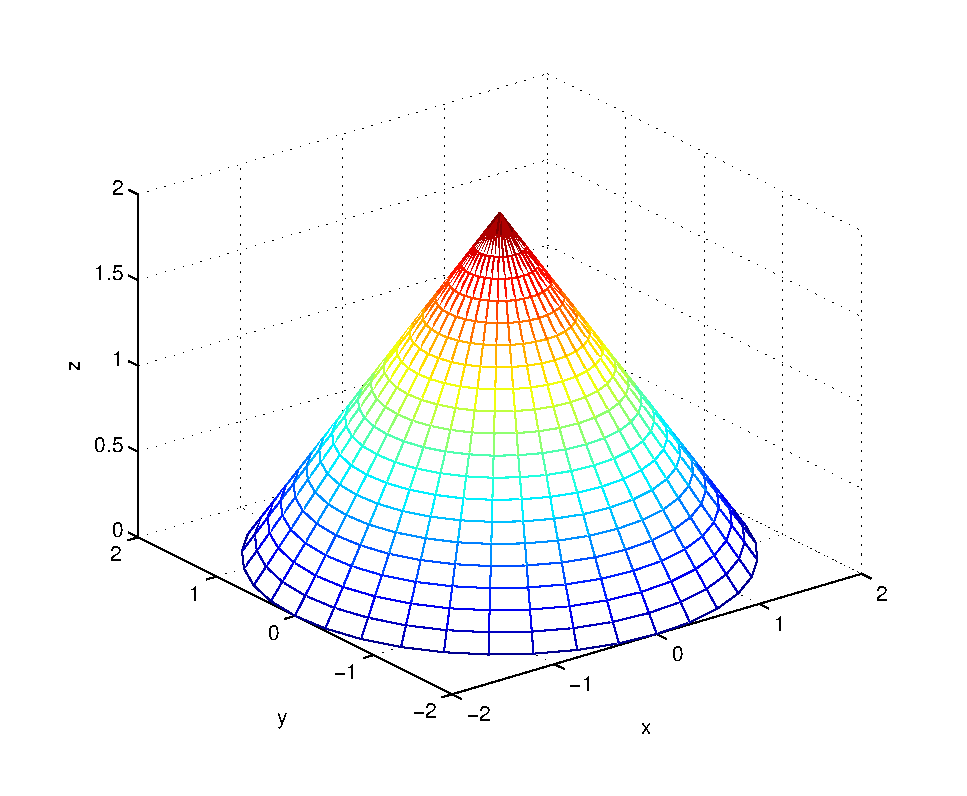
\includegraphics[width=12cm]{cono.eps}
\caption{Cono representado sobre una ret�cula circular}
\label{fig:cono}
\end{figure}

A continuaci�n, se incluye el c�digo de un script con varios ejemplos m�s de dise�o de ret�culas circulares y gr�ficos de superficies en 3D. Los resultados se muestran en la figura \ref{fig:varios}

\lstinputlisting{../codigo/matlab/introduccion/varios_g3d.m}

\begin{figure}[h]
\centering
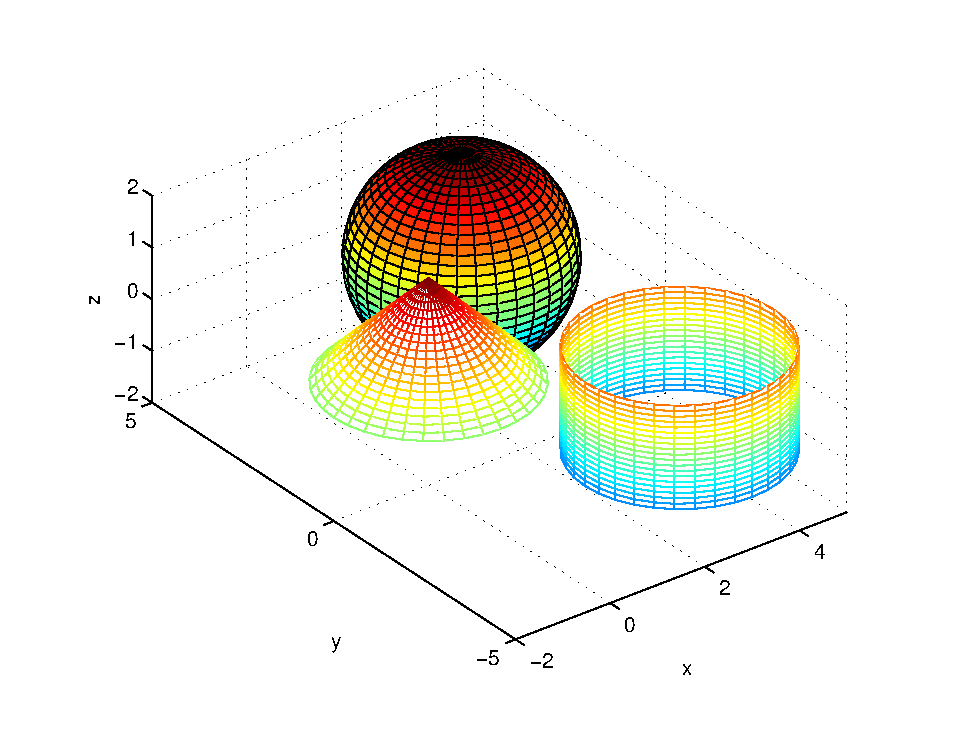
\includegraphics[width=12cm]{varios.eps}
\caption{ret�cula con simetr�a circular}
\label{fig:varios}
\end{figure}

\paragraph{contour, contour3, meshc y surfc.} Este comandos permiten obtener y dibujar las curvas de nivel de una superficie. Su uso es id�ntico al de los comandos anteriores. Es decir, tambi�n necesitan que se defina una ret�cula en el plano $(x,y)$, y se calculen los valores que tomar�  la variable z sobre los puntos de la ret�cula.

\begin{figure}
\centering
\subfigure[contour  \label{fig:contour}]{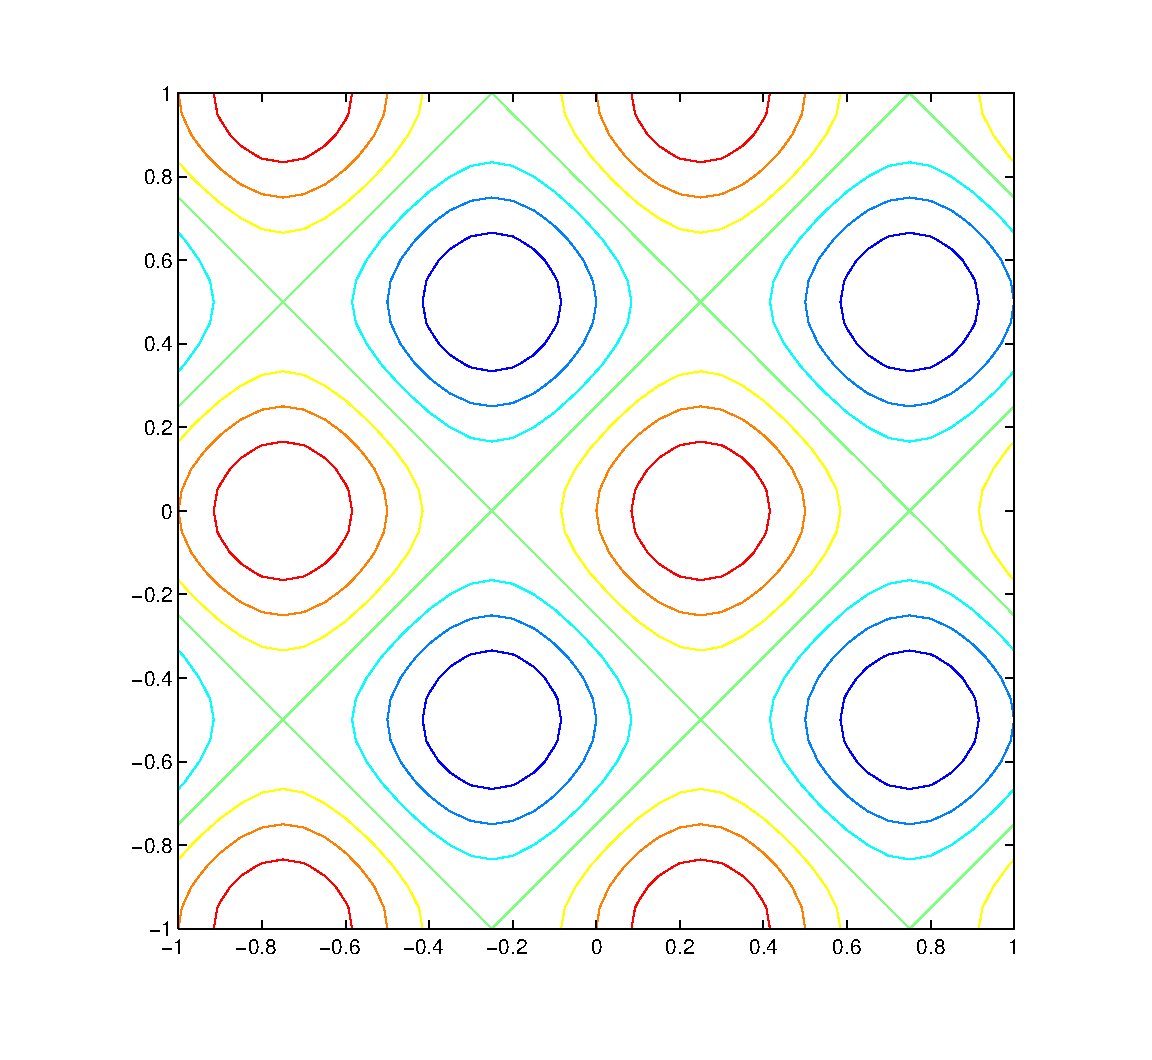
\includegraphics[width=6.5cm]{contour.eps}} \qquad 
\subfigure[contour3 \label{fig:contour3}]{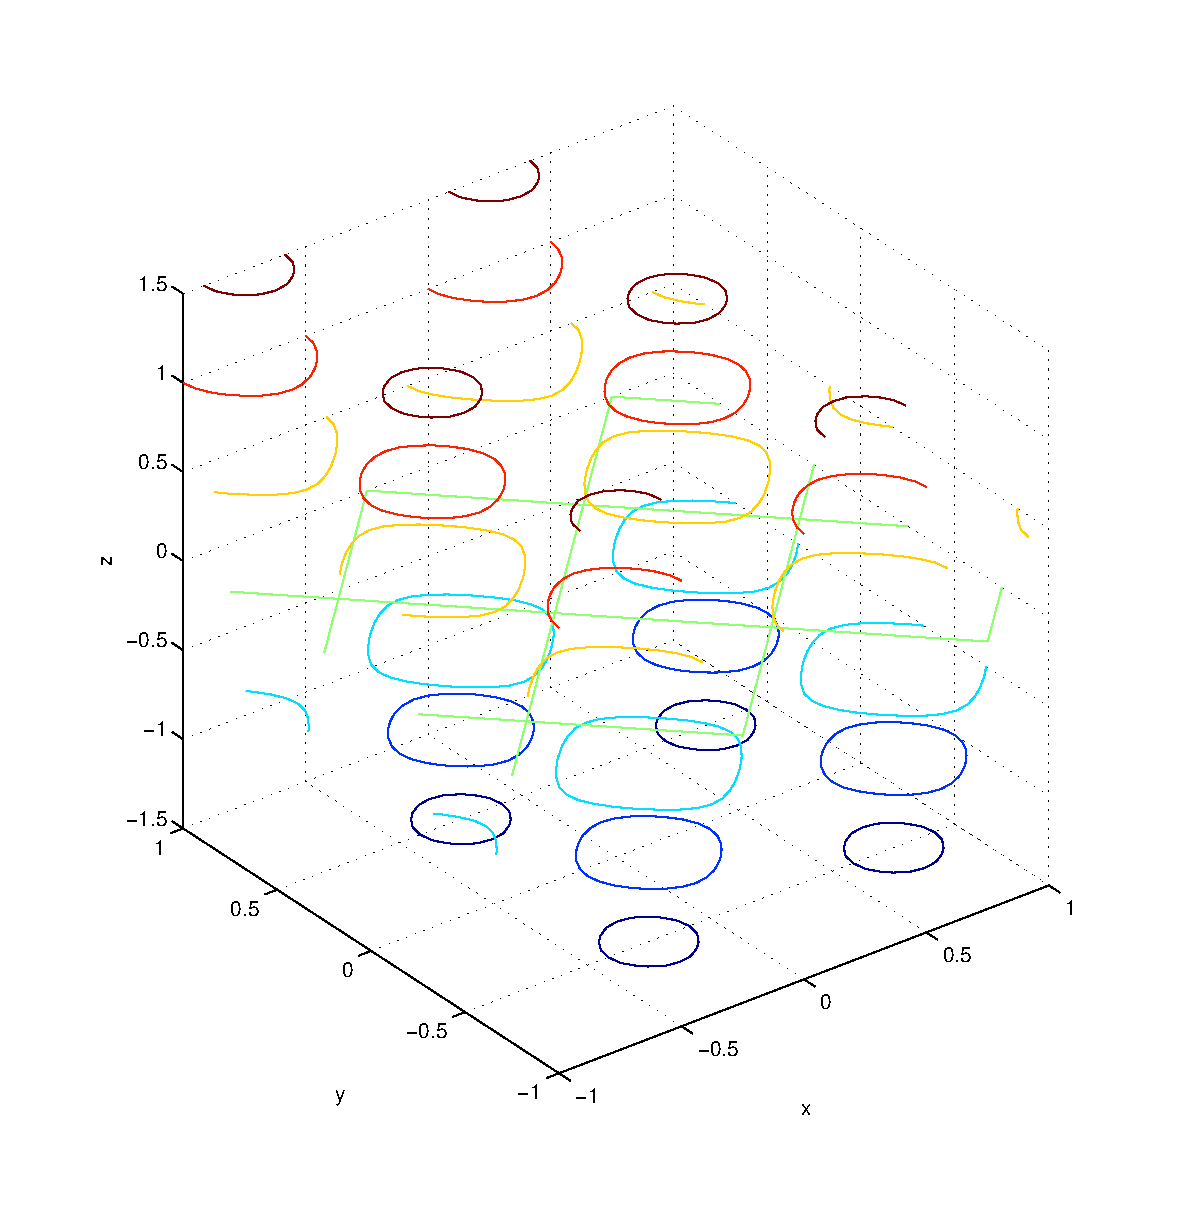
\includegraphics[width=6.5cm]{contour3.eps}}\\
\subfigure[meshc \label{fig:mesh3}]{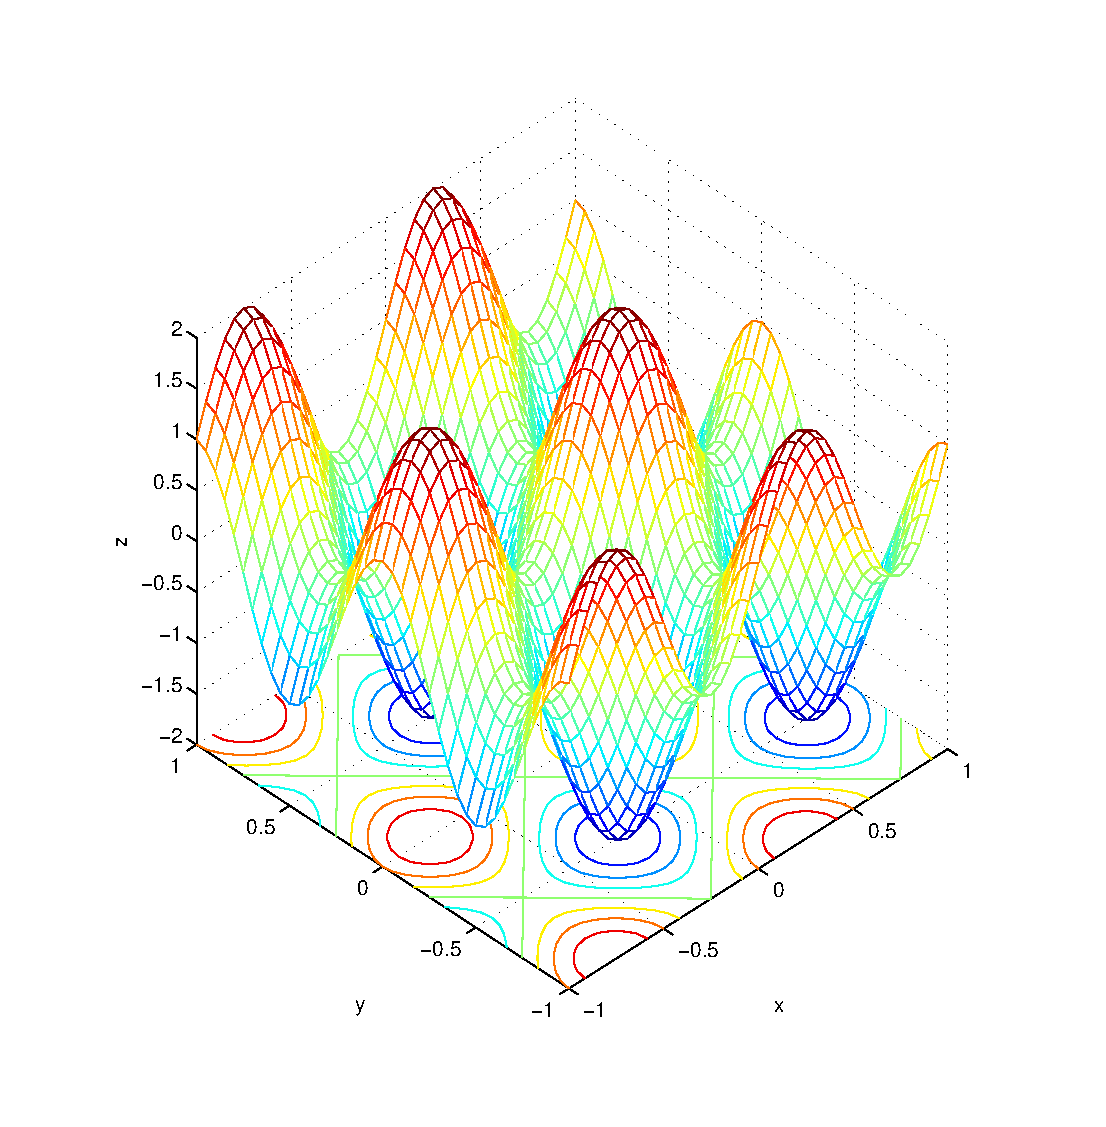
\includegraphics[width=6.5cm]{meshc.eps}}\qquad
\subfigure[surfc \label{fig:surf3}]{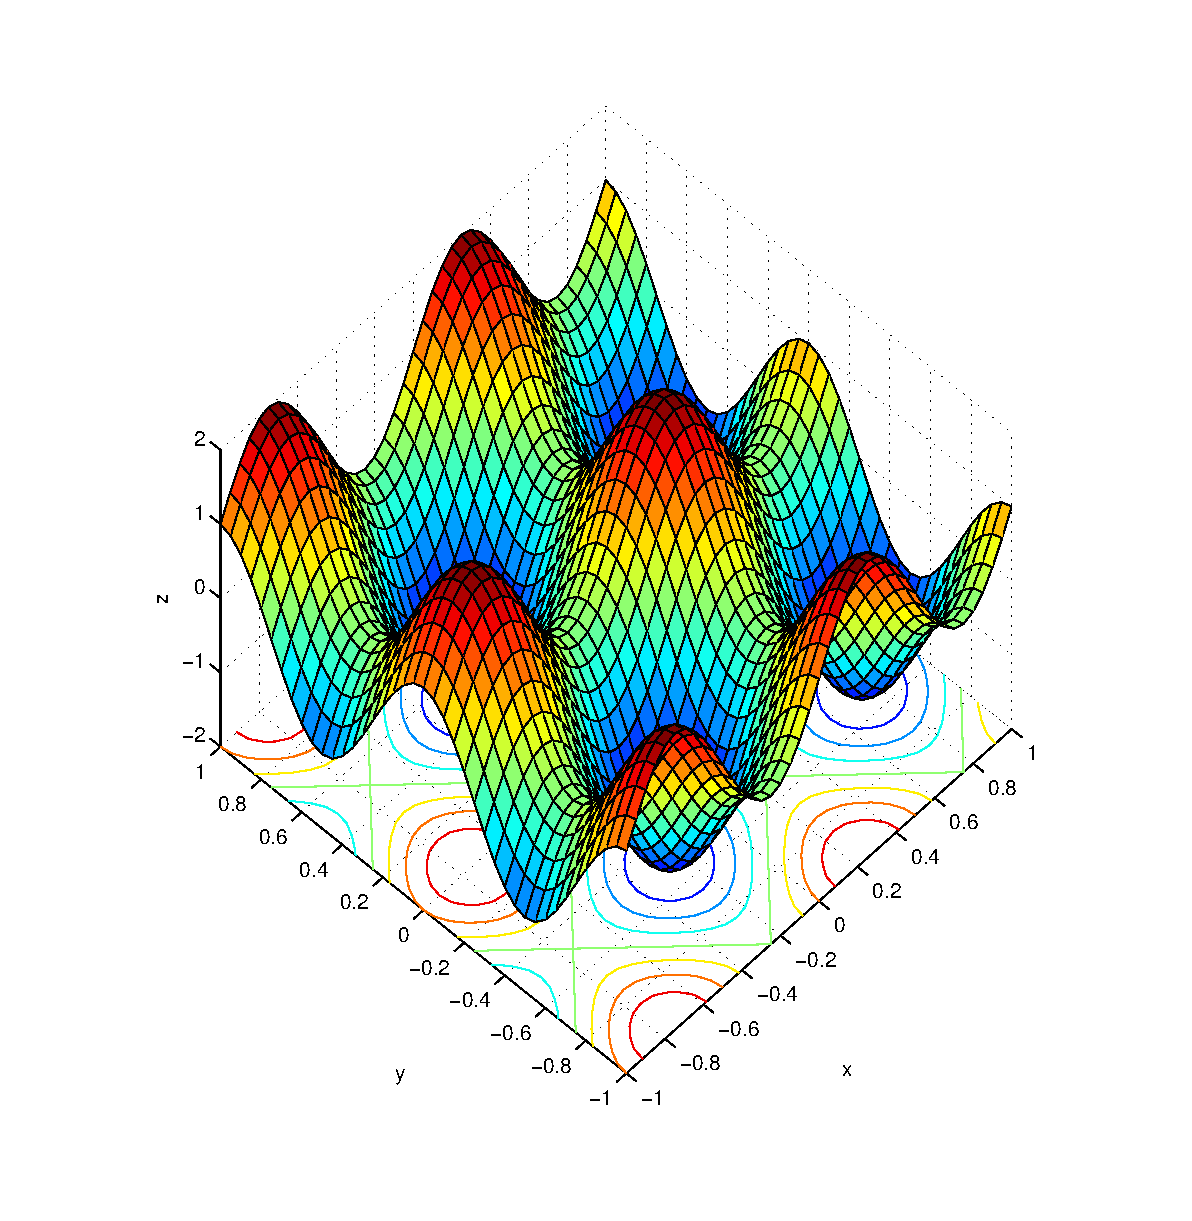
\includegraphics[width=6.5cm]{surfc.eps}}\\
\caption{Comparaci�n entre los resultados de \texttt{contour}, \texttt{contour3}, \texttt{meshc} y \texttt{surfc}, para la obtenci�n de las curvas de nivel de una superficie. }
\end{figure}

Veamos su funcionamiento con un �ltimo ejemplo. Obtenemos una ret�cula cuadrada, calculamos sobre ella los puntos de la superficie,

\begin{equation*}
z=\sin(2\pi x)+cos(2\pi y)
\end{equation*}

\begin{verbatim}
>> x=[-1:0.05:1];
>> y=x;
>> [xm,ym]=meshgrid(x,y);
>> zm=sin(2*pi*xm)+cos(2*pi*ym);
>> contour(xm,ym,zm)
>> contour3(xm,ym,zm)
>> meshc(xm,ym,zm)
>> surfc(xm,ym,zm)
\end{verbatim}



La figura \ref{fig:contour} muestra los resultados de aplicar el comando \texttt{contour}. La gr�fica representa las curvas de nivel de la superficie dibujadas sobre el plano $(x,y)$. El comando \texttt{contour3} ( figura \ref{fig:contour3}) representa de nuevo las curvas de nivel, pero sit�a cada una a su correspondiente altura $z$.  Por �ltimo \texttt{meshc} y \texttt{surfc} representan la superficie y a�aden en el plano $(x,y)$ la representaci�n de las curvas de nivel correspondiente a la superficie.

Para terminar la secci�n dedicada a los gr�ficos, vamos a combinar el comando \texttt{mesh} con el comando \texttt{plot3} para dibujar una curva sobre una superficie. Tomaremos como ejemplo la superficie,
\begin{equation*}
z=\frac{sin\left((\pi x)^2+(\pi y^2)\right)}{(\pi x)^2+(\pi y^2)}
\end{equation*}

Sobre la que trazamos la curva,

\begin{equation*}
y=sin(\pi x),\\
\end{equation*}

\begin{figure}[h]
\centering
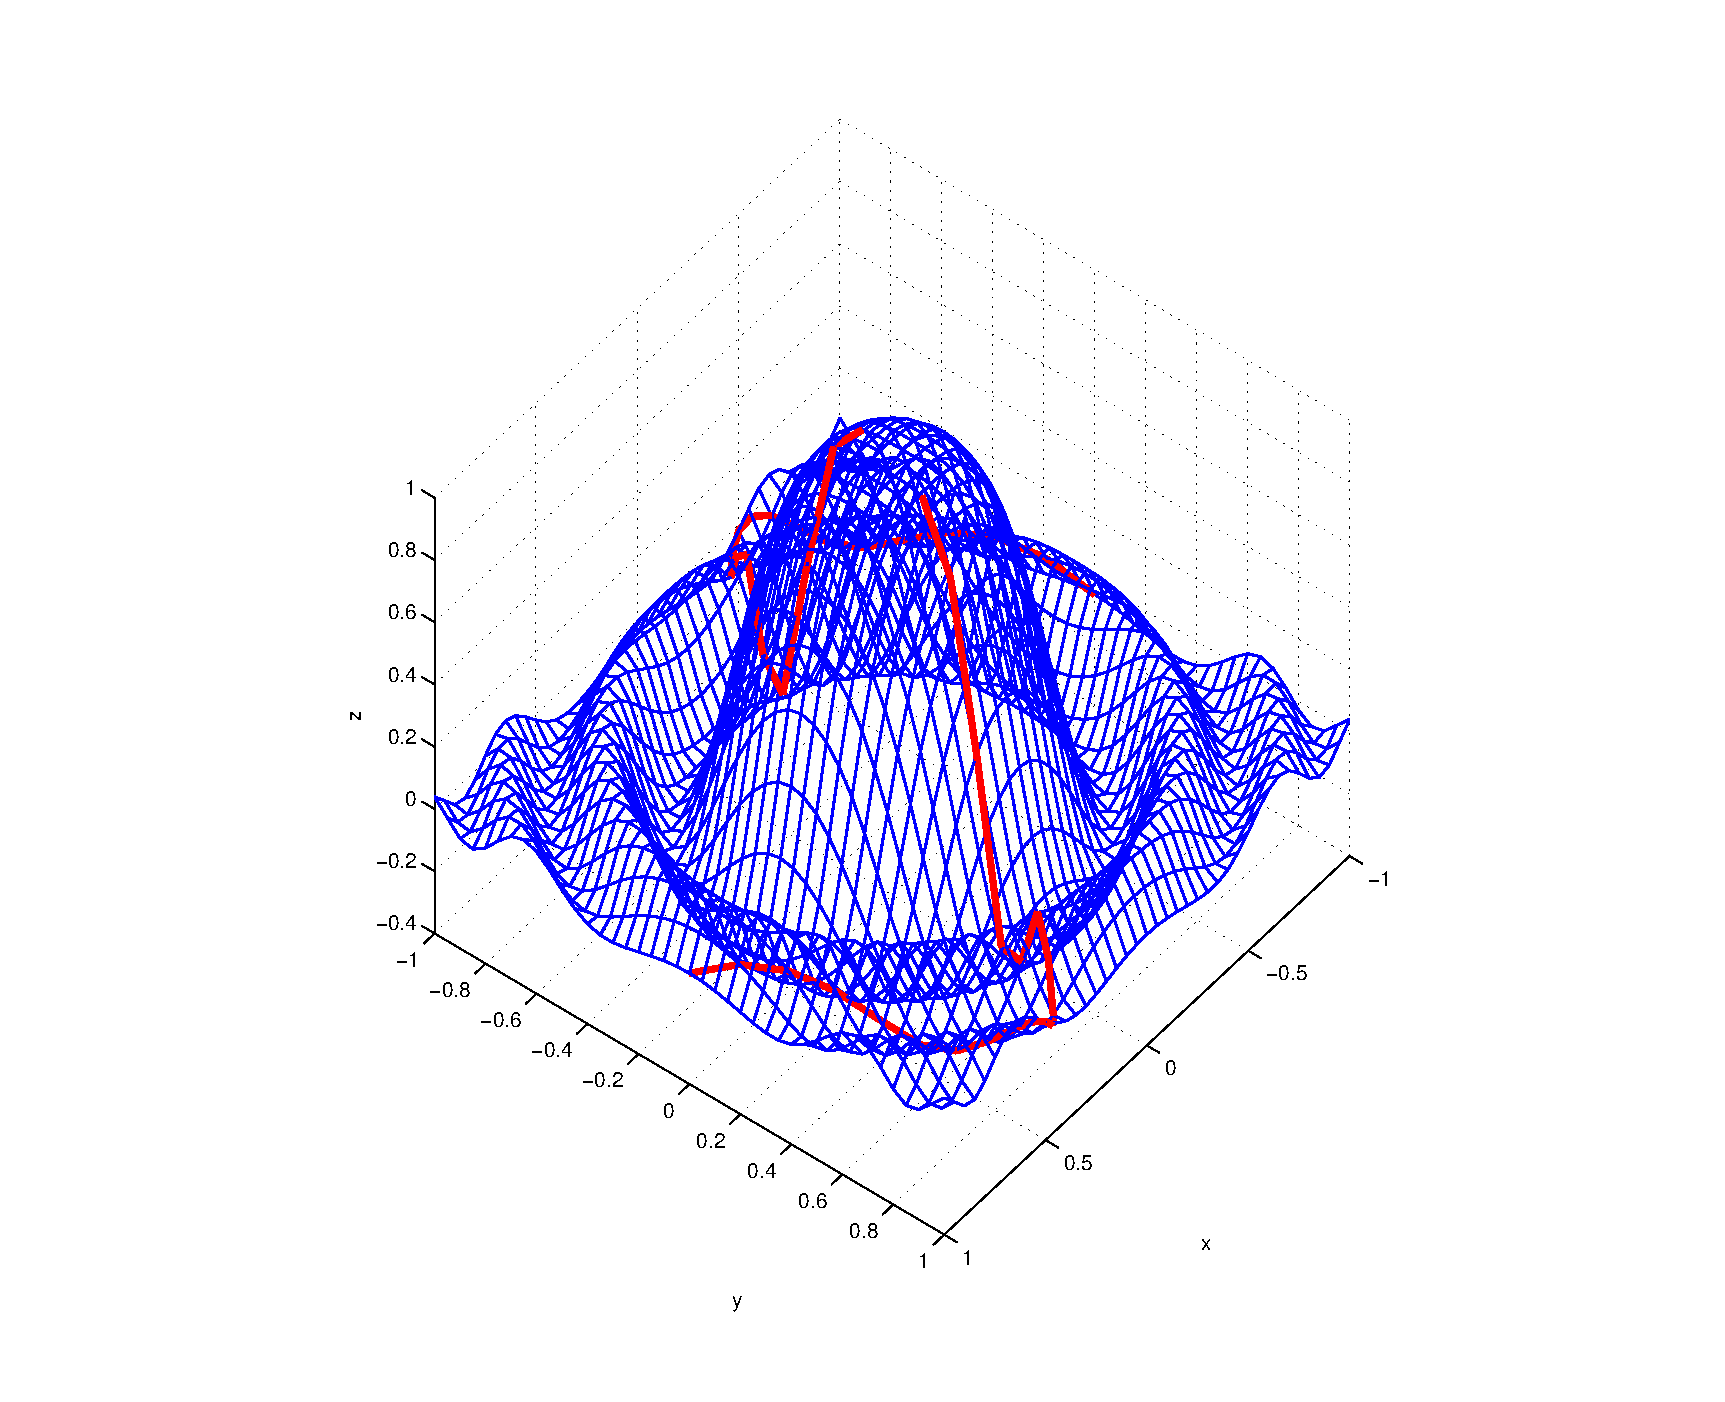
\includegraphics[width=11cm]{linsu.eps}
\caption{Curva trazada sobre una superficie}
\label{fig:cvsurf}
\end{figure}

Es decir, obtenemos el valor de los puntos $z$ de la superficie para los pares de puntos $[x, y = sin(\pi x)]$, que definen la curva trazada sobre la superficie $z$,

\begin{verbatim}
>> x=[-1:0.05:1];
>> y=x;
>> [xm,ym]=meshgrid(x,y);
>> zm=sin((pi*xm).^2+(pi*ym).^2)./((pi*xm).^2+(pi*ym).^2);
>> mesh(xm,ym,zm)
>> y=sin(pi*x);
>> z=sin((pi*x).^2+(pi*y).^2)./((pi*x).^2+(pi*y).^2);
>> hold on
>> plot3(x,y,z)
\end{verbatim}

Es importante insistir en que a lo largo de esta secci�n nos hemos limitado a introducir algunas de las posibilidades gr�ficas de Matlab. Para obtener una visi�n completa de las mismas es imprescindible leer con detenimiento la ayuda de Matlab.

\newpage
\section{Ejercicios}
\begin{enumerate}
\item Tipos de variables en Matlab; matrices y vectores. Escribe, por orden, las siguientes expresiones en la \emph{l�nea de comandos} de Matlab e interpreta los resultados que obtienes. En los casos en que Matlab devuelva un mensaje de error, trata de averiguar la raz�n. \textbf{Nota:} Es importante hacerlos por orden ya que algunos operaciones se apoyan en los resultados de operaciones anteriores.
\begin{multicols}{2}
\begin{enumerate}
\renewcommand{\labelenumii}{\arabic{enumii}}
\texttt{
\item a=[1 2 3; 4 5 6]
\item a=[1 2 3; 4 5]
\item a=[ 1 2 3\\
1 2 3\\
1 2]
\item[*] Operador (:) para crear vectores
\item a=[1:10:0]
\item a=1:10:2
\item a=1:0.05:2
\item a=1:-0.05:-1
\item a=[1:10;2:12;3:13]
\item a=[1:10;2:11;3:12]
\item a=[1 2 7\\
5 6 8\\
3 2 6]
\item b=[1 2 3]
\item c=[a b]
\item c=[a;b]
\item d=[b;a]
\item[*] Operador (:) para indexar
\item c=[a(1,:) b]
\item c=[a(1:2,:);b]
\item c=[a(1:2,:);b;a(size(a,1),:)]
\item[*] Funciones para manipulaci�n de matrices
\item a=[1 2 3]
\item b=diag(a)
\item c=diag(b)
\item M=size(c)
\item \ [m,n]=size(c)
\item m=size(c)
\item m=size(c,1)
\item m=size(c,2)
\item d=ones(size(a))
\item d=ones(size(b))
\item  d=ones(size(b,1))
\item d=ones(size(b,1),size(c,2))
\item f=eye(size(d,1))
\item who
\item whos
\item clear all
\item who
\item q=[1 2 3\\
4 5 6\\
7 8 9]
\item  r=diag(q,1)
\item  r=diag(q,2)
\item  r=diag(q,0)
\item  r=diag(q,-1)
\item  r=diag(q,-2)
\item  tt=eye(1,3)
\item  tt=eye(3,1)
\item  tt=eye(3)
\item  tt=eye(5)
\item  tt=eye(5,3)\\
\item  tt=eye(3,5)\\
\item a=[1 3 4\\
2 4 6]\\
\item  b=[2 3\\
4 5\\
6 7]
\item[*] Operadores aplicados a matrices
\item c=a*b
\item d=b*a
\item e=[ 1 2\\
4 5]
\item a*e
\item g=a*e
\item g=e*a
\item a*b
\item a=[1 3 4\\
5 6 8]
\item b=3
\item a*b
\item a.*b
\item b=[2 3]
\item a.*b
\item b=[ 2 3 4\\
5 6 7]
\item a.*b
\item c=b'
\item d=a'
\item r=a-b
\item h=a-a'
\item j=a+b
\item j=a'+b
\item d=(a+b)*b'
\item f=(a+b)*b'
\item f=(a-b)'*b
\item a=[ 1 3 5\\
2 5 6
3 4 2]
\item p=a\^{}2
\item r=a\^{}2-a*a
\item r=a.\^{}2-a*a
\item r=a\^{}2-a.*a
\item b=[ 3 5 6\\
2 1 1\\
1 2 3]
\item[*] Encadenando operaciones
\item w=a*b\^{}(-1)
\item w=a*inv(b)
\item w=a/b
\item w= a*b\^{}(-1)-a*inv(b)
\item w= a*b\^{}(-1)-a/b
\item w=a\^{}(-1)*b
\item w=inv(a)*b
\item w=a\textbackslash b
\item w= a\^{}(-1)*b-inv(a)*b
\item w=a\textbackslash b-inv(a)*b
\item w=a./b
\item w=a.\textbackslash b
\item w=a.\^{}(-1)*b
\item w=a.\^{}(-1)*b-a.\textbackslash b
}
\end{enumerate}
\end{multicols}
\item Obt�n empleando la \emph{l�nea de comandos} de matlab el resultado de las siguientes expresiones:
\begin{multicols}{2}
\begin{align*}
\frac{5+3x^2}{6y}\\
\frac{1+4\sqrt{2x}}{6}y \\
\frac{-x+\sqrt{x^2-4xy}}{2x}
\end{align*}

\begin{align*}
\frac{1}{\sqrt{2\pi}}e^{-\frac{1}{2}(x-1)^2}\\
\sin^2(2x)+\cos^2(2x) \\
\arctan(\infty)\\
\arctan\left(\frac{y}{x}\right)
\end{align*}
\end{multicols}
Emplea para $x$ e $y$ tanto valores escalares como matrices.

\item Abre un fichero nuevo en el editor de textos de matlab.
Escribe las siguiente l�neas:\\
\texttt{
x = A*B\\
y = A+B\\
z = A*sin(B)}\\
Guarda el fichero. Emplea el comando \verb|clear| all para limpiar el \emph{workspace}
Invoca el fichero desde matlab. �Qu� sucede?\\
Crea en la ventana de comandos las matrices,
\begin{equation*}
A =\begin{pmatrix}
1&3&4\\
2&5&6\\
7&8&9
\end{pmatrix}, \ B=\begin{pmatrix}
2&6&8\\
3&7&8\\
2&7&9
\end{pmatrix}
\end{equation*}
Vuelve a ejecutar el programa guardado en el fichero.\\
A�ade al programa, al principio del todo, la l�nea \texttt{clear all}. Guarda y vuelve a ejecutar el
programa. �Qu� sucede ahora?\\
Introduce las matrices A y B directamente en el c�digo del programa debajo de la l�nea \texttt{clear all}. Analiza qu� sucede al ejecutar de nuevo el programa.\\
 Eliminar la l�nea \texttt{clear all}. Introduce a trav�s de la ventana de comando dos matrices $A$ y $B$ distintas de las que contiene el programa. Ejecuta el programa y comprueba qu� matrices utiliza para realizar los c�lculos.\\
Comenta la(s) l�nea(s) de c�digo donde has definido las matrices $A$ y $B$ en el programa. A�ade al principio del programa una l�nea para convertir el script en una funci�n:\\
\verb|function [x] = nombre_de_tu_programa(A,B)| \\
Invoca la funci�n reci�n creada desde la \emph{l�nea de comandos} de matlab. Observa lo que pasa si la invocas como:
\begin{verbatim}
>>nombre_de_tu_programa
>>nombre_de_tu_programa(F)
>>nombre_de_tu_programa(F,J)
\end{verbatim}
Introduce, en el  workspace de matlab --usando la \emph{l�nea de comandos}--  las matrices $F$ y $J$, dondo,
\begin{equation*}
F =\begin{pmatrix}
1&0&1\\
2&0&4\\
3&5&0
\end{pmatrix}, \ J=\begin{pmatrix}
1&6&7\\
2&9&0\\
4&4&4
\end{pmatrix}
\end{equation*}
Vuelve a ejecutar, \verb|>>nombre_de_tu_programa(F,J)| \\
Genera dos matrices de tama�o $(3\times 3)$. N�mbralas como prefieras: \verb|mi_matriz1, mi_matriz2|. Ejecuta ahora,
\begin{verbatim}
>>nombre_de_tu_programa(mi_matriz1,J)
>>nombre_de_tu_programa(mi_matriz2,F)
>>nombre_de_tu_programa(mi_matriz1,mi_matriz2)
>>resultado=nombre_de_tu_programa(F,J)
>>[r1,r2]=nombre_de_tu_programa(F,J)
>>[A,B;r3]=nombre_de_tu_programa(F,J)
>>[A,B;C]=nombre_de_tu_programa(A,B)
\end{verbatim}
Crea un nuevo fichero, con el siguiente c�digo:
\begin{lstlisting}
A=sin(B).*cos(C)
[D,E,F]=nombre_de_tu_programa(A,C)
G = D + E - F
\end{lstlisting}
Gu�rdalo con el nombre que quieras.\\
Define en la \emph{l�nea de comandos} matrices $B$ y $C$ adecuadas para el programa que acabas de escribir y ejec�talo.\\
A�ade al programa una primera l�nea de c�digo que lo convierta en una funci�n que tome como entradas las matrices $B$ y $C$  y que:\\
devuelva solo la matriz $G$\\
devuelva las matrices $G$ y $D$\\ 
devuelva las matrices $G$,$D$,$E$ y $F$.

Escribe una nueva funci�n con el siguiente c�digo,
\begin{lstlisting}
function A=nombre_de_la_funcion(B,C)
E=B + C^2;
D=B - inv(C);
A=nombre_funcion_dentro(E,D);
end;
function s=nombre_funcion_dentro(l,p);
s=l + p - 2;
end;
\end{lstlisting}
Crea matrices $B$ y $C$ adecuadas y ejecuta la funci�n que acabas de crear. Describe c�mo funciona.

\item Define en la \emph{l�nea de comandos} las matriz $M$ y $N$ e interpreta el resultado de las condiciones l�gicas impuestas.

\begin{equation*}
M =\begin{pmatrix}
1&2&3\\
4&5&6\\
7&8&9
\end{pmatrix}, \ N=\begin{pmatrix}
2&3&4\\
5&6&7\\
8&9&10
\end{pmatrix}
\end{equation*}
\begin{verbatim}
>>y=m<2
>>y=m<=2
>>y=m>2
>>y=m>=2
>>y=m==2
>>y=m~=2
>>y=any(m<2)
>>y=any(m<2,1)
>>y=any(m<2,2)
>>y=any(m==2)
>>y=all(m>=2)
>>y=all(m~=0)
>>y=all(any(m<2))
>>y=any(all(m<2))

>> index=find(m>2)
>>[i,j]=find(m<5)

>> y=any(m<2)&any(n>4)
>> y=any(m<2)&any(n>10)
>> y=any(m<2)&any(n>6)
>> y=any(m<2)&any(n>7)
>> y=any(m<2)&any(n>3)
>> y=any(m<2)&any(n>2)
>> y=any(m>2)&any(n>2)
>> y=any(m>4)&any(n>2)
>> y=any(m>4,1)&any(n>2)
>> y=any(m>4,2)'&any(n>2)
\end{verbatim}
Repite el estudio de las condiciones l�gicas cambiando \& por \textbar

\item Escribe el siguiente c�digo en un fichero. Ejec�talo y analiza los resultados,
\begin{lstlisting}
dato=rand(1)
if dato==0.5
 dato=0
elseif dato<0.5
 dato=-dato*10
else
 dato=dato*10
end
\end{lstlisting}

Modifica el programa,
\begin{enumerate}
\item Para que no muestre los resultados de los c�lculos por pantalla
\item para que, utilizando comandos \verb|elseif, &| devuelva una variable (distinta de 'dato') con valor $-1$ si se cumple que 'dato' es menor o igual que $0.3$, con valor $-0.5$ si 'dato' es mayor que $0.3$ y menor que $0.5$, con valor $0$ si 'dato' es mayor o igual que $0.5$ y menor  o igual que $0.7$ y con valor $1$ en cualquier otro caso.
\item Convierte el \emph{script}, en una funci�n, que tome 'dato' como variable de entrada, y devuelva el valor de la variable obtenida, seg�n la condici�n que se cumpla. (L�gicamente se debe eliminar o comentar la l�nea \verb|dato=rand(1)|).
\end{enumerate}

\item Crea un scrip de matlab con el siguiente c�digo y trata de adivinar qu� hace antes de ejecutarlo. Utiliza el \emph{help} de matlab para averiguar lo que hace la funci�n \verb|abs|.
\begin{lstlisting}
n=10
for i=1:n
 for j=1:n
  if i==j
   a(i,j)=1;
  elseif abs(i-j)==1
   a(i,j)=-1
  else
   a(i,j)=0
  end
 end
end
\end{lstlisting}

Introduce un punto de ruptura (\emph{breakpoint}) en el c�digo, por ejemplo en la l�nea 12. Ejecuta paso a paso el programa para ver como va generando el resultado. Intercambia los �ndices \verb|i,j| de la matriz \verb|a|. \verb|a(j,i)|.�Se obtiene el mismo resultado? �C�mo se construye ahora la matriz?

\item Crea un script con el siguiente c�digo,
\begin{lstlisting}
i=0
while(i<10)
 i=i+1
 j=0
while(j<10)
  j=j+1
  if i==j
   a(i,j)=1;
  elseif abs(i-j)==1
   a(i,j)=-1
  else
   a(i,j)=0
  end
 end
end
\end{lstlisting}
Repite el estudio del programa anterior

\item Modifica el \emph{script} anterior de modo que quede el siguiente c�digo,
\begin{lstlisting}
i=0
while(1)
 i=i+1
 j=0
 while(1)
  j=j+1
  if i==j
   a(i,j)=1;
  elseif abs(i-j)==1
   a(i,j)=-1
  else
   a(i,j)=0
  end
  if j==10
   break
  end
 end
 if i==10
  break
 end
end
\end{lstlisting}
Repite el estudio del programa anterior. �Qu� sucede si comentamos la(s) l�nea(s) que contiene la sentencia \verb|break|?
Reconvierte los \emph{scrips} anteriores en funciones que admitan como variable de entrada el tama�o de la matriz que se desea generar y devuelvan como variable de salida la matriz creada.

\item Dada una matriz $A \in \mathbb{R}^{n\times n}$ y un vector columna $v \in \mathbb{R}^n-{\mathbf{0}}$. Se dice que el vector $v$ pertenece al \emph{Kernel} de $A$ si se cumple que $Av =\mathbf{0}$.



Crea una funci�n que tome como variables de entrada una matriz $A$ cuadrada de cualquier dimension $n\times n$ y un vector columna de dimensi�n $n$ y compruebe si$n$ pertenece o no al \emph{kernel} de $A$. \textbf{Nota:} Considera que la condici�n se cumple si todos los elementos del vector $Av$ son menores que $1e-12$.

\item Escribe ---empleando bucles y sin hacer uso del operador ( \^\ ) --- una funci�n \verb|potencia.m| que reciba como argumentos de entrada un n�mero real $x\in \mathbb{R}$ y un entero $n \in \mathbb{Z}$ y devuelva el valor de la n-�sima potencia de $x$ ($x^n$). El segundo argumento de entrada puede ser opcional. Si se omite debe tomarse como $n=2$ (devolviendo el cuadrado de $x$). Ver la funci�n interna nargin. \textbf{Nota:} Ten en cuenta que $n$ puede ser positivo, negativo o cero.

\item Crea una funci�n que determine la suma de los inversos de los n�meros naturales impares menores de 1000. Usa las funciones tic y toc para determinar el tiempo que se tarda. Emplea bucles para el c�lculo.
\begin{equation*}
S_{imp} = \sum_{n=1}^{500}\frac{1}{2n-1} =\frac{1}{1}+\frac{1}{3}+\frac{1}{5}+\cdots+\frac{1}{999}
\end{equation*}
Modifica tu programa, de modo que admita como variable de entrada un n�mero $m\in\mathbb{N}$ y calcule el valor de la suma de los inversos de los impares menores o iguales que $m$.

\item Los n�meros de Fibonacci, $F(n)$ son una serie de n�meros naturales. Los dos primeros valores de la serie son:  $F(1)=1$ y $F(2)=2$. Los dem�s t�rminos se calculan como la suma de los dos anteriores: $F(n) = F(n-1) + F(n-2)$.
Escribe un script que genere los primeros $m$ n�meros de la serie de Fibonacci, almacen�ndolos en un vector \verb|F|. Emplea para el c�lculo la estructura \verb|while|.

\item Sin utilizar las funciones de matlab \verb|flip,fliplr, flipud,...|, escribe las l�neas de c�digo para que, dado un vector \verb|x|, genere otro vector con el orden de los elementos invertido.
\end{enumerate}

\section{Test del curso 2020/21}
\begin{enumerate}

\item  El movimiento de un cuerpo en el plano viene descrito por las siguientes ecuaciones,

\begin{align}
x(t) &= \sin(2 \pi \, \omega_1 t)\\
y(t) &= \cos(2 \pi \, \omega_2 t)\\
z(t) &= a\cos(2\pi \, \omega_1 t) \label{eq:3}
\end{align}

donde $x,y,z$ representan las coordenadas del cuerpo en el instante de tiempo $t$ medidas en metros,  $w_1$ y $w_2$ son frecuencias fijas medidas en $rad\cdot s^{-1}$ y $a$ es una amplitud fija medida en metros.

\begin{enumerate}
	\item \label{ap1} (\textbf{1.5 puntos}) Escribe una funci�n que:

\begin{enumerate}
	\item Tome como variables de entrada las frecuencias $w_1$, $w_2$, la amplitud $a$ .
	\item Haga el c�lculo de la trayectoria en tres dimensiones descrita por el cuerpo en el intervalo de tiempo $[0,1]$. Considera incrementos de tiempo de $0.01s$.
	\item Dibuje en una gr�fica la trayectoria descrita por el cuerpo en el espacio. Cada eje del gr�fico deber� llevar  una etiqueta indicando de qu� variable se trata $x$, $y$ � $z$.
	\item La salida ser�n tres vectores con los valores de $x$, $y$ y $z$ calculados para cada instante de tiempo.
	\end{enumerate}

\item (\textbf{1.5 puntos}) A�ade a la funci�n creada en el apartado anterior el c�digo necesario para que:
	\begin{enumerate}
	\item \textbf{Solo si} se le dan dos variables de entrada en lugar de tres, entonces calcule la trayectoria que describir�a el cuerpo en el plano si se eliminara la ecuaci�n (\ref{eq:3}) de las ecuaciones del sistema. (NOTA: La funci�n debe seguir funcionando igual que en el apartado anterior si se le dan tres entradas. Emplea el comando nargin).
	\item El resultado deber� tambi�n representarse gr�ficamente, pero solo en dos dimensiones, y devolver la variable $z$ como un vector vac�o. 
	\end{enumerate}

\item \label{ap2} (\textbf{1.5 puntos}) Crea un un \emph{live script} que genere dos  vectores de frecuencias: \texttt{W1} y \texttt{W2} de  modo que el primero contenga los n�meros impares comprendidos entre $1$ y $7$ y el segundo los n�meros pares comprendidos entres $2$ y $8$.  Emplea la funci�n creada en el apartado anterior para calcular el valor de las trayectorias obtenidas tomando como entradas para  $\omega_1, \omega_2$,  todos los pares posibles de la forma: \texttt{W1(i)} y \texttt{W2(j)}. Sup�n que no hay tercera entrada $a$. Realiza los c�lculos empleando bucles.

\item (\textbf{1 punto}) A�ade a tu programa el c�digo necesario para que dibuje cada resultado en un \emph{subplot} de modo que la figura resultante tenga $4\times4$ \emph{subplots} (ver figura al dorso).  Debes crear los \emph{subplots} empleando los mismos bucles del apartados anterior. 

\item (\textbf{0.5 puntos}) Repite los c�lculos de los apartados c) y d) pero tomando ahora $a=1$.
\end{enumerate}

\item Una matriz cuadrada $A$, de dimensi�n arbitraria $(n\times n)$, cuyos elementos $a_{ij} \in \mathbb{Z}$, se define como \emph{buenrollista} cuando las suma de los valores pares de cada fila es mayor o igual que la suma de los valores  impares de la columna correspondiente, i.e., satisface la siguiente relaci�n:
\begin{equation}
	\sum_{j=1}^n a_{ij\text{(par)}} \geq \sum_{j=1}^n a_{ji\text{(impar)}}, \quad \forall i\in\{1,...,n\}
\end{equation}

\begin{enumerate}
\item (\textbf{1.5 puntos}) Escribe  una funci�n que tome como variable de entrada una matriz cuadrada de cualquier dimensi�n 
y calcule un vector con las sumas de los valores pares de los elementos de cada una de su filas  y otro vector con las sumas de los elementos impares de cada una de sus columnas.
\item (\textbf{1.5 puntos}) A�ade a la funci�n anterior el c�digo necesario para que compruebe, empleando los vectores obtenidos en el apartado anterior, si la funci�n es \emph{buenrollista} y muestre un mensaje por pantalla indicando si lo es o no.
\item (\textbf{1 punto}) Aplica la funci�n desarrollada a la siguiente matriz:
\begin{equation*}
\begin{pmatrix}
2&3&4&6&1\\
5&4&-2&3&0\\
4&-1&5&4&-6\\
4&2&4&5&8\\
3&0&-3&-3&6
\end{pmatrix}
\end{equation*}
\end{enumerate}
\end{enumerate}
\noindent\rule{\textwidth}{0.4pt}
\begin{figure}[h]
\centering
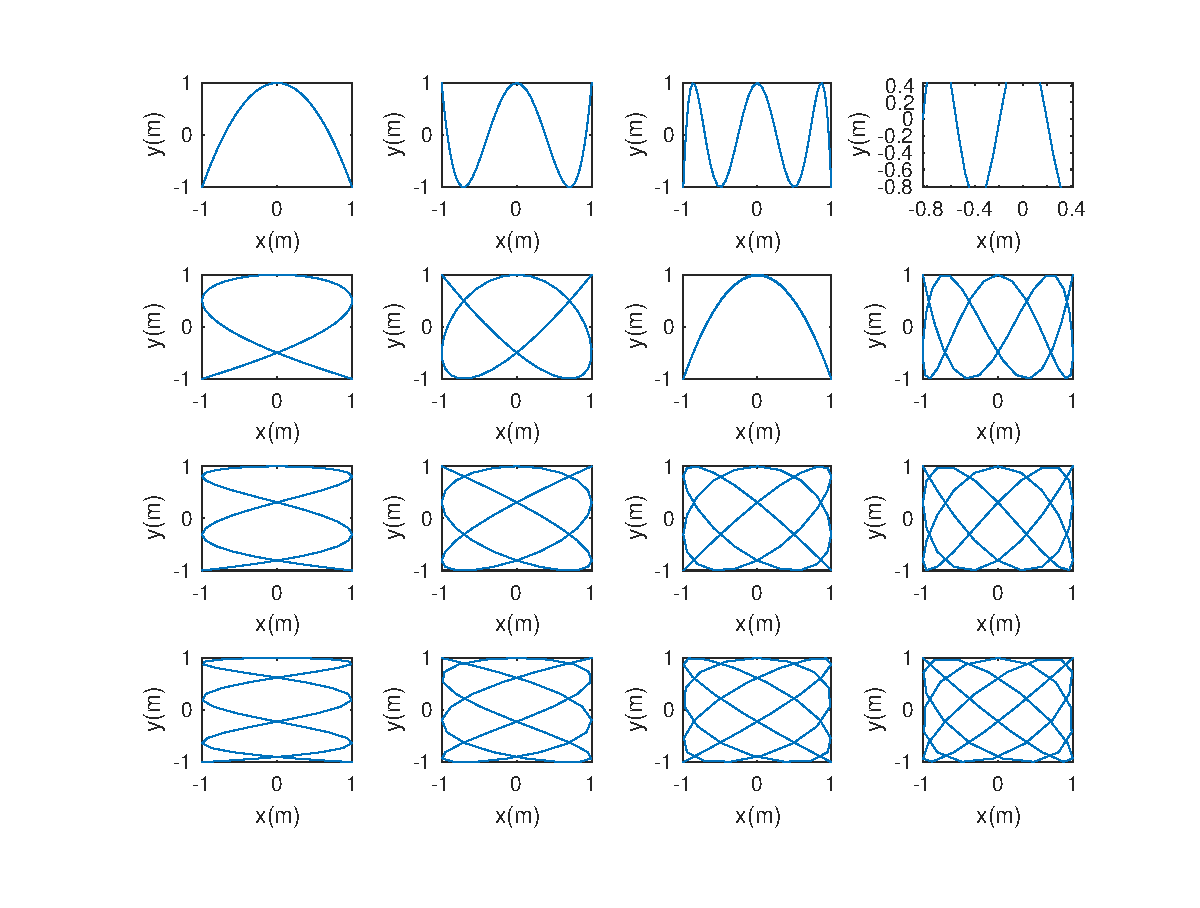
\includegraphics[scale=0.5]{lisa1.eps}
\caption{vista de la figura con los ocho subplots} \label{fig:1}
\end{figure}

\section{Test del curso 2021/22}
\begin{enumerate}

\item  Una part�cula cargada de masa $m$ y carga $q$ parte del origen con velocidad inicial

\begin{align}
x(t) &= \sin(2 \pi \, \omega_1 t)\\
y(t) &= \cos(2 \pi \, \omega_2 t)\\
z(t) &= a\cos(2\pi \, \omega_1 t) \label{eq:3}
\end{align}

donde $x,y,z$ representan las coordenadas del cuerpo en el instante de tiempo $t$ medidas en metros,  $w_1$ y $w_2$ son frecuencias fijas medidas en $rad\cdot s^{-1}$ y $a$ es una amplitud fija medida en metros.

\begin{enumerate}
	\item \label{ap1} (\textbf{1.5 puntos}) Escribe una funci�n que:
	
	\begin{enumerate}
		\item Tome como variables de entrada las frecuencias $w_1$, $w_2$, la amplitud $a$ .
		\item Haga el c�lculo de la trayectoria en tres dimensiones descrita por el cuerpo en el intervalo de tiempo $[0,1]$. Considera incrementos de tiempo de $0.01s$.
		\item Dibuje en una gr�fica la trayectoria descrita por el cuerpo en el espacio. Cada eje del gr�fico deber� llevar  una etiqueta indicando de qu� variable se trata $x$, $y$ � $z$.
		\item La salida ser�n tres vectores con los valores de $x$, $y$ y $z$ calculados para cada instante de tiempo.
	\end{enumerate}
	
	\item (\textbf{1.5 puntos}) A�ade a la funci�n creada en el apartado anterior el c�digo necesario para que:
	\begin{enumerate}
		\item \textbf{Solo si} se le dan dos variables de entrada en lugar de tres, entonces calcule la trayectoria que describir�a el cuerpo en el plano si se eliminara la ecuaci�n (\ref{eq:3}) de las ecuaciones del sistema. (NOTA: La funci�n debe seguir funcionando igual que en el apartado anterior si se le dan tres entradas. Emplea el comando nargin).
		\item El resultado deber� tambi�n representarse gr�ficamente, pero solo en dos dimensiones, y devolver la variable $z$ como un vector vac�o. 
	\end{enumerate}
	
	\item \label{ap2} (\textbf{1.5 puntos}) Crea un un \emph{live script} que genere dos  vectores de frecuencias: \texttt{W1} y \texttt{W2} de  modo que el primero contenga los n�meros impares comprendidos entre $1$ y $7$ y el segundo los n�meros pares comprendidos entres $2$ y $8$.  Emplea la funci�n creada en el apartado anterior para calcular el valor de las trayectorias obtenidas tomando como entradas para  $\omega_1, \omega_2$,  todos los pares posibles de la forma: \texttt{W1(i)} y \texttt{W2(j)}. Sup�n que no hay tercera entrada $a$. Realiza los c�lculos empleando bucles.
	
	\item (\textbf{1 punto}) A�ade a tu programa el c�digo necesario para que dibuje cada resultado en un \emph{subplot} de modo que la figura resultante tenga $4\times4$ \emph{subplots} (ver figura al dorso).  Debes crear los \emph{subplots} empleando los mismos bucles del apartados anterior. 
	
	\item (\textbf{0.5 puntos}) Repite los c�lculos de los apartados c) y d) pero tomando ahora $a=1$.
\end{enumerate}

\item Una matriz cuadrada $A$, de dimensi�n arbitraria $(n\times n)$, cuyos elementos $a_{ij} \in \mathbb{Z}$, se define como \emph{buenrollista} cuando las suma de los valores pares de cada fila es mayor o igual que la suma de los valores  impares de la columna correspondiente, i.e., satisface la siguiente relaci�n:
\begin{equation}
\sum_{j=1}^n a_{ij\text{(par)}} \geq \sum_{j=1}^n a_{ji\text{(impar)}}, \quad \forall i\in\{1,...,n\}
\end{equation}

\begin{enumerate}
	\item (\textbf{1.5 puntos}) Escribe  una funci�n que tome como variable de entrada una matriz cuadrada de cualquier dimensi�n 
	y calcule un vector con las sumas de los valores pares de los elementos de cada una de su filas  y otro vector con las sumas de los elementos impares de cada una de sus columnas.
	\item (\textbf{1.5 puntos}) A�ade a la funci�n anterior el c�digo necesario para que compruebe, empleando los vectores obtenidos en el apartado anterior, si la funci�n es \emph{buenrollista} y muestre un mensaje por pantalla indicando si lo es o no.
	\item (\textbf{1 punto}) Aplica la funci�n desarrollada a la siguiente matriz:
	\begin{equation*}
	\begin{pmatrix}
	2&3&4&6&1\\
	5&4&-2&3&0\\
	4&-1&5&4&-6\\
	4&2&4&5&8\\
	3&0&-3&-3&6
	\end{pmatrix}
	\end{equation*}
\end{enumerate}
\end{enumerate}



\section{Test del curso 2022/23}
\begin{enumerate}
	
	
	
	
	\item Las ecuaciones param�tricas que definen el movimiento de una part�cula en el espacio son las siguientes:
	\begin{align*}
	x &= r\cdot\sin(t)\\
	y &= r\cdot\cos(t) \\
	z &= 2\cdot t
	\end{align*}
	
	Donde $t \in \mathbb{R}^+$ representa el tiempo transcurrido desde el inicio del movimiento, $x,y,z \in \mathbb{R}$ son las coordenadas del vector posici�n de la part�cula en $\mathbb{R}^3$ y $r \in \mathbb{R}$ representa un par�metro fijo.
	
	\begin{enumerate}
		\item \label{ap5} (\textbf{1 punto}) Para $r=4$ y $0\leq t \leq 10\cdot \pi$ dibuja la trayectoria de la part�cula en el espacio. Pon t�tulo a la gr�fica y etiquetas a todos los ejes.
		\item \label{ap6} (\textbf{1 punto}) Empleando el comando \textit{subplot}, dibuja la trayectoria de la part�cula para cada uno de los valores de $r=[1 ,4 ,8 ,12]$. Pon t�tulo a cada gr�fica.
		\item \label{ap6} (\textbf{2 puntos}) Usando el comando \textit{quiver3} dibuja el vector de la velocidad de la part�cula para $t=[\pi, 2 \pi, 4\pi ,6\pi]$ en la gr�fica de $r=12$. Recuerda que $v_x=\frac{dx}{dt}$, $v_y=\frac{dy}{dt}$ y $v_z=\frac{dz}{dt}$
		
	\end{enumerate}
	
	\item  Una terna pitag�rica es un conjunto de tres n�meros $a, b, c \in \mathbb{Z}^+ \vert a^2+b^2=c^2$. La terna se llama primitiva si el m�ximo com�n divisor de $a,b\  \text{y}\ c$ es $1$ 
	
	Dados dos n�meros $m,n \in \mathbb{Z}^+ \vert m>n$ Si construimos $a$, $b$ y $c$ como,
	\begin{align*}
	a &=m^2 -n^2\\
	b &= 2m\cdot n\\
	c &= m^2 + n^2\\
	\end{align*}
	constituyen una terna pitag�rica. Si adem�s $m$ y $n$ son coprimos ($m$ no es divisible por $n$) y uno de ellos es par, la terna resultante es una terna primitiva\footnote{El �ltimo teorema de Fermat, postulado por Pierre de Fermat alrededor de 1637, plantea que no existen ternas no triviales an�logas a las ternas pitag�ricas, para exponentes mayores que dos. Es decir La ecuaci�n $x^n+y^n=z^n$
		no tiene soluci�n si $n>2$ con $x$, $y$, $z$, $n$ naturales. Sin demostraci�n durante m�s de 300 a�os, Andrew Wiles consigui� demostrarlo en 1995.}.
	
	\begin{enumerate}
		\item \label{ap1}(\textbf{1 punto}) Escribe una funci�n en matlab que tome como variable de entrada dos n�meros enteros positivos $m,n : m>n$, y devuelva como variable de salida un vector $v= [a, b, c, d]$ de modo que los tres primeros valores correspondan a los valores $a,b,c$ de la terna pitag�rica generada por $m$ y $n$. El cuarto valor del vector, $d$, valdr� $1$ si la terna generada es primitiva y $0$ en caso contrario. 
		El programa deber� comprobar que las variables de entrada cumplen la condici�n $m>n$ y si no la cumplen terminar la ejecuci�n y dar un mensaje de error.
		\item (\textbf{1 punto}) Crea una segunda funci�n que llame a la del apartado \ref{ap1}) y calcule las ternas pitag�ricas para $n$ un n�mero par cualquiera y los $l$ primeros n�meros primos mayores que $n$. Los resultados deber� devolverlos en una matriz de dimensi�n $l\times 3$ en la que cada fila contendr� los elementos $a,b,c$ de cada una de las ternas generadas. Obt�n la matriz resultante para $n=4$ y $l=10$. \textbf{Puedes usar la funci�n \textit{isprime} de matlab, pero en ese caso este apartado valdr� $0.5$ puntos en lugar de 1. }
	\end{enumerate}
	
	\item Tenemos el siguiente grafo $\mathcal{G = \mathcal(V,A)}$ que describe las conexiones de la futura l�nea de metro de N�menor. 
	\begin{figure}[h]
		\centering
		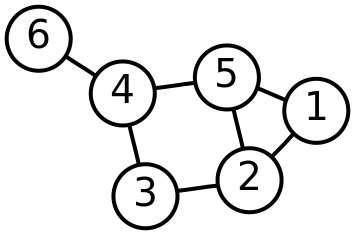
\includegraphics[width=0.3\textwidth]{grafo.png}
	\end{figure}
	
	Cada estaci�n se ha representado como un v�rtice del grafo, $\mathcal{V} = \{1,2,3,4,5,6\}$. Las conexiones directas entre dos estaciones se representan como aristas que unen los correspondientes v�rtices, $\mathcal{A}=\{\cdots,(i,j),\cdots\}\vert i,j \in \mathcal{V}$. Adem�s, el grafo se considera no dirigido, es decir, $(i,j)\in \mathcal{A} \Rightarrow (j,i) \in \mathcal{A}$. Podemos describir este grafo con una matriz (que se llama \textbf{matriz Laplaciana})  de la siguiente manera:
	\begin{equation}
	l_{i,j}=\left\{
	\begin{array}{ll}
	\kappa_i  & \mbox{si } i =j \\
	-1 & 		\mbox{si } i \neq j \mbox{ e } i \mbox{ es adyacente a } j\\
	0 & \mbox{en otro caso}
	\end{array}
	\right.
	\end{equation}
	donde $\kappa_i$ es el grado del v�rtice $i$, es decir, el n�mero de aristas que salen de dicho v�rtice.
	
	
	\begin{enumerate}
		\item \label{ap1} (\textbf{1 punto}) Escribe la matriz laplaciana del grafo del futuro metro de N�menor.
		\item \label{ap3} (\textbf{1 punto}) La matriz de adyacencia de un grafo es una matriz $ \mathcal{B}$ donde cada elemento $b_{i,j}=1$ si y solo si existe una arista entre los v�rtices $i$ y $j$, en otro caso $b_{i,j}=0$. Crea una funci�n que, dada la matriz laplaciana de un grafo, devuelva la matriz de adyacencia $ \mathcal{B}$. 
		\item \label{ap4} (\textbf{1 punto}) Crea tambi�n una funci�n que dada la matriz de adyacencia de un grafo devuelva su matriz laplaciana. 
		\item \label{ap2} (\textbf{1 punto}) Por construcci�n, la suma de los elementos de cada fila de una matriz laplaciana es cero. Adem�s en una matriz laplaciana los elementos que no est�n en la diagonal s�lo pueden valer $0$ � $-1$. Programa una funci�n que dada una matriz cualesquiera compruebe estas dos condiciones anteriores. Si se cumplen ha de devolver un vector con los elementos de la diagonal y si no se cumplen un vector de ceros adecuado a las dimensiones de la matriz introducida.
		
	\end{enumerate}
	%
\end{enumerate}

\chapter{Aritm�tica del Computador y Fuentes de error}
En el cap�tulo 1, introdujimos la representaci�n binaria de n�meros as� como la conversi�n de binario a decimal y decimal a binario. A lo largo de este cap�tulo vamos a profundizar m�s en el modo en que el ordenador representa y opera con los n�meros as� como en una de sus consecuencias inmediatas: la imprecisi�n de los resultados. 

\section{Representaci�n binaria y decimal}\index{Binario}

Los n�meros reales pueden representarse empleando para ello una recta que se extiende entre $-\infty$ y $+\infty$. La mayor�a de ellos no admiten una representaci�n num�rica exacta, puesto que poseen infinitos decimales. 

Los n�meros enteros, $1, -1, 2, -2, 3, -3, \cdots$ admiten una representaci�n num�rica exacta. \index{Notaci�n cient�fica} En cualquier caso, rara vez manejamos n�meros enteros con una cantidad grande de d�gitos, habitualmente, los aproximamos, expres�ndolos en notaci�n cient�fica, multiplic�ndolos por una potencia de $10$. Tomemos un ejemplo de la qu�mica: la cantidad de �tomos o mol�culas que constituyen un mol de una sustancia se expresa por el n�mero de Avogadro, $N_A=6.02214179 \times 10^{23}$, dicho numero, --que deber�a ser un entero--  se expresa empleando tan solo 9 de sus 23 cifras significativas (a veces tan solo se dan las tres primeras). 

\index{Truncamiento} Cuando truncamos un n�mero, es decir, despreciamos todos sus d�gitos hacia la derecha a partir de uno dado, estamos aproximando dicho n�mero por un  n�mero racional, es decir, por un n�mero que puede expresarse como el cociente entre dos n�meros enteros. $1/2, 3/4, \cdots$ 

Algunos n�meros racionales se reducen a su vez a n�meros enteros, $6/3$, otros dan lugar a n�meros cuya representaci�n exige un n�mero finito de d�gitos: 
\begin{equation*}
11/2=(5.5)_{10}=5\times10^0+5\times10^{-1}
\end{equation*} 
Si representamos el mismo n�mero en base 2 obtenemos,
\begin{equation*}
11/2=(101.1)_2=1\times2^2+0\times2^1+1\times2^0+1\times2^{-1}
\end{equation*}
Sin embargo, el que un n�mero racional admita una representaci�n finita, depende de la base en que se representa. Por ejemplo: $1/10=(0.1)_{10}$ no admite representaci�n finita en base 2.
\begin{equation*}
1/10=(0.0001100110011\cdots)_2 =1\times2^{-4}+1\times2^{-5}+0\times2^{-6}+0\times2^{-7}+1\times2^{-8}+\cdots 
\end{equation*}
 
En este �ltimo caso, se trata de una representaci�n que, aunque no termina, es repetitiva o peri�dica; tras el primer cero decimal se repite indefinidamente la secuencia: $0011$. Los n�meros racionales admiten siempre una representaci�n finita � infinita peri�dica. 

El n�mero racional $1/3=(0.333\cdots)_{10}=(0.010101\cdots)_2$ solo admite representaci�n infinita peri�dica tanto en base 10 como en base 2. Sin embargo, admite representaci�n finita si lo representamos en base 3: $1/3=(0.1)_3=0\times3^0+1\times3^{-1}$.

Habitualmente, en la vida ordinaria, representamos los n�meros en base 10, sin embargo, como hemos visto en el cap�tulo 1 el ordenador emplea una representaci�n binaria. Como acabamos de ver, una primera consecuencia de esta diferencia, es que al pasar n�meros de una representaci�n a otra estemos alterando la precisi�n con la que manejamos dichos n�meros. Esta diferencia de representaci�n supone ya una primera fuente de errores, que es preciso tener en cuenta cuando lo que se pretende es hacer c�lculo cient�fico con un ordenador. Como iremos viendo a lo largo de este cap�tulo, no ser� la �nica.

\section{Representaci�n de n�meros en el ordenador}\index{Representaci�n num�rica}
\paragraph{Enteros positivos} La forma mas f�cil de representar n�meros ser�a empleando directamente los registros de memoria para guardar n�meros en binario.  Si suponemos un ordenador que tenga regis-\- tros de 16 bits. Podr�amos guardar en ellos n�meros comprendidos entre el $0$ y el $2^{16}-1=65535$. Este �ltimo se representar�a con un $1$ en cada una de las posiciones del registro, en total 16 unos. Se trata del entero m�s grande que podr�amos representar con un registro de 16 bits:
\\

\begin{tabular}{|l|c|c|c|c|c|c|c|c|c|c|c|c|c|c|c|c|}
\hline
posici�n&1&2&3&4&5&6&7&8&9&10&11&12&13&14&15&16  \\
\hline
valor&1&1&1&1&1&1&1&1&1&1&1&1&1&1&1&1 \\
\hline
\end{tabular}\\

 Hasta ahora, nuestro sistema de representaci�n solo admite n�meros enteros. El menor n�mero que podemos representar es el cero, y el mayor ---depender� del tama�o $n$ de los registros del ordenador---, $2^n-1$.  Es evidente que este sistema de representaci�n resulta insuficiente.
 
 \paragraph{Enteros positivos y negativos}
 Un primera mejora consistir�a en ampliar el sistema de representaci�n para que admita tambi�n n�meros negativos. Una posibilidad ser�a reservar uno de los bits del array para representar el signo \index{Bit de signo}, y usar los restantes para representar el n�mero. En nuestro ejemplo de un registro de 16 bits, el n�mero m�s grande ser�a ahora $2^{15}-1$ y el m�s peque�o ser�a $-2^{15}+1$. El cero tendr�a una doble representaci�n, una de ellas con signo m�s y la otra con signo menos.
 
 Una representaci�n alternativa, cuyo uso est� muy extendido en las m�quinas, es la representaci�n conocida con el nombre de \emph{Complemento a 2} \index{Complemento a dos} \index{Representaci�n num�rica!}. Supongamos un registro de n bits:
 \begin{itemize}
 \item Un entero $x$ no negativo se almacena empleando directamente su representaci�n binaria. el intervalo de enteros no negativos representables es: $0 \le x \le 2^{(n-1)}-1$.
 \item Un entero negativo $-x$, donde $1 \le x \le 2^{(n-1)}$, se almacena como la representaci�n binaria del entero positivo: $2^{n}-x$
 \item El n�mero as� construido,  recibe el nombre de complemento a 2 de x.
 \end{itemize}
 En general, dado un n�mero entero $N<2^n$ su complemento a dos en una representaci�n binaria de $n$ d�gitos se define como:
 \begin{equation*}
 C_2^N=2^n-N
 \end{equation*} 
 Veamos un ejemplo de esta representaci�n, para el caso de un registro de 4 bits:
 
 \begin{table}
 \centering
 \begin{tabular}{r  l  r  r}
 Decimal&  (4 bits) &\ $C_2=2^n-x$ & n. representado\\
 \hline
15& 1111&$(16-1)=15$&-1\\
14& 1110&$(16-2)=14$&-2\\
13& 1101&$(16-3)=13$&-3\\
12& 1100&$(16-4)=12$&-4\\
11& 1011&$(16-5)=11$&-5\\
10& 1010&$(16-6)=10$&-6\\
9& 1001& $(16- 7)=9$&-7\\
8& 1000& $(16-8)=8$&-8\\
\hline
\hline
7& 0111& & 7\\
6& 0110& & 6\\
5& 0101& & 5\\
4& 0100& & 4\\
3& 0011& & 3\\
2& 0010& & 2\\
1& 0001& & 1\\
0& 0000& & 0\\
\hline
\end{tabular}
 \end{table}
 

 La representaci�n en complemento a 2 tiene las siguientes caracter�sticas:
 \begin{itemize}
 \item La representaci�n de los n�meros positivos coincide con su valor binario
 \item La representaci�n del n�mero 0 es �nica.
 \item El rango de valores representables en una representaci�n de N bits es $-2^{N-1} \le x \le  2^{N-1}-1$.
 \item Los n�meros negativos se obtienen como el complemento a dos, cambiado de signo,  del valor binario que los representa. 
 \end{itemize}

Una forma pr�ctica de obtener el complemento a dos de un n�mero binario es copiar el n�mero original de  derecha a izquierda hasta que aparezca el primer 1. Luego de copiar el primer 1, se complementan el resto de los bits del n�mero (si es 0 se pone un 1 y si es 1 se pone un 0). Por ejemplo el complemento a dos del n�mero 2, (0010 en una representaci�n de 4 bits) ser�a 1110,

\begin{eqnarray*}
001\mathbf{0} & \xrightarrow{copia\  bit\ derecha }& \cdots 0 \\
00\mathbf{1}0 & \xrightarrow{copia\ primer\ bit = 1}& \cdot \cdot 10\\ 
0 \mathbf{0}10& \xrightarrow{complemento\ bit\  0} &\cdot  \ 110\\
 \mathbf{0}010& \xrightarrow{complemento\ bit\ 0} &1110
\end{eqnarray*} 

\index{Complemento a dos! Sustracci�n} Una propiedad importante de la representaci�n de complemento a dos, es que la diferencia de dos n�meros puede realizarse directamente sumando al primero el complemento a dos del segundo. Para verlo podemos usar los dos n�meros del ejemplo anterior: $0010$ es la representaci�n binaria del n�mero $2$, si empleamos un registro de cuatro bits. Su complemento a dos, $1110$ representa al n�mero $-2$. Si los sumamos \index{Adici�n en binario} \footnote{Sumar en binario es como sumar en decimal. Se procede de bit a bit, de derecha a izquierda y cuando se suman 1 y 1, el resultado es 10 (base 2), de modo que el bit resultante se coloca en 0 y se lleva el 1 hacia el siguiente bit de la izquierda.}:

\begin{table}
 \centering
\begin{tabular}{|c|c|c|c|c|}
\hline
 &0&0&1&0\\
 \hline
  &1&1&1&0\\
  \hline
  \textbf{1}&0&0&0&0\\
  \hline
  \hline
  &0&0&0&0\\
  \hline
\end{tabular}
\end{table}

El resultado de la suma nos da un n�mero cuyos primeros cuatro bits son 0. El bit distinto de cero, no puede ser almacenado en un registro de cuatro bits, se dice que el resultado de la operaci�n \emph{desborda} el tama�o del registro. Ese bit que no puede almacenarse se descarta al realizar la operaci�n de suma, con lo que el resultado ser�a cero, como corresponde a la suma de $2+(-2)$. Esta es la motivaci�n fundamental para emplear una representaci�n en complemente a dos: No hace falta emplear circuitos especiales para calcular la diferencia entre dos n�meros, ya que �sta se representa como la suma del minuendo con el complemento a dos del sustraendo.

\subsection{N�meros no enteros: Representaci�n en punto fijo y en punto flotante}
La representaci�n de n�meros no enteros se emplea para representar de modo aproximado n�meros reales. Como hemos dicho antes, los n�meros racionales peri�dicos y los n�meros irracionales no pueden representarse de forma exacta mediante un n�mero finito de decimales. Por esta raz�n, su representaci�n es siempre aproximada. Para los n�meros racionales no peri�dicos, la representaci�n ser� exacta o aproximada dependiendo del n�mero que se trate, el tama�o de los registros del ordenador y el sistema empleado para la representaci�n. Los dos sistemas de representaci�n m�s conocidos son la representaci�n en  punto fijo y, de especial inter�s para el c�lculo cient�fico, la representaci�n en punto flotante.

\paragraph*{Representaci�n en punto fijo.} \index{Representaci�n num�rica! en punto fijo}En la representaci�n en punto fijo, el registro empleado para almacenar un n�mero se divide en tres partes: 
\begin{itemize}
\item 1 bit para almacenar el signo del n�mero.  
\item Un campo de bits de tama�o fijo para representar la parte entera del n�mero.
\item Un campo para almacenar la parte decimal del n�mero
\end{itemize}

Por ejemplo, si tenemos un registro de 16 bits podemos reservar 1 bit para el signo, 7 para la parte entera y 8 para la parte decimal.  La representaci�n en punto fijo del n�mero binario $-10111.0011101101$ ser�a: \\


\begin{tabular}{|c||c|c|c|c|c|c|c||c|c|c|c|c|c|c|c|}
\hline
s&\multicolumn{7}{c||}{p. entera}&\multicolumn{8}{c|}{p. decimal}\\
\hline
1&0&0&1&0&1&1&1&0&0&1&1&1&0&1&1\\
\hline
\end{tabular}\\

Es interesante notar c�mo para representar la parten entera, nos sobran dos bits en el registro, ya que la parte entera solo tiene cinco cifras y tenemos 7 bits para representarla. Sin embargo, la parte decimal tiene 10 cifras; como solo tenemos 8 bits para representar la parte decimal, la representaci�n trunca el n�mero eliminando los dos �ltimos decimales.

Si asociamos cada bit con una potencia de dos, en orden creciente de derecha a izquierda, podemos convertir directamente el n�mero representado de binario a decimal,\\ 

\begin{tabular}{|c||c|c|c|c|c|c|c||c|c|c|c|c|c|c|c|}
\hline
s&\multicolumn{7}{c||}{p. entera}&\multicolumn{8}{c|}{p. decimal}\\
\hline
1&0&0&1&0&1&1&1&0&0&1&1&1&0&1&1\\
\hline
-&$2^{6}$&$2^{5}$&$2^{4}$&$2^{3}$&$2^{2}$&$2^{1}$&$2^{0}$&$2^{-1}$&$2^{-2}$&$2^{-3}$&$2^{-4}$&$2^{-5}$&$2^{-6}$&$2^{-7}$&$2^{-8}$\\
\hline
\end{tabular}\\

Por tanto el n�mero representado ser�a,

\begin{equation*}
\begin{split}
&-(0\cdot 2^6+0 \cdot 2^5+ 1\cdot 2^4+ 0 \cdot 2^3+ 1 \cdot 2^2 + 1 \cdot 2^1 + 1 \cdot 2^0 + 0 \cdot 2^{-1}+ 0 \cdot 2^{-2}+ 1 \cdot 2^{-3}+ 1 \cdot 2^{-4}+ \\
& +1 \cdot 2^{-5}+0 \cdot 2^{-6} +1 \cdot 2^{-7}+1 \cdot {-8}) = - 23.23046875
\end{split}
\end{equation*}

De modo an�logo podemos calcular cual ser�a el n�mero m�s grande representable,\\

\begin{tabular}{|c||c|c|c|c|c|c|c||c|c|c|c|c|c|c|c|}
\hline
s&\multicolumn{7}{c||}{p. entera}&\multicolumn{8}{c|}{p. decimal}\\
\hline
0&1&1&1&1&1&1&1&1&1&1&1&1&1&1&1\\
\hline
&$2^{6}$&$2^{5}$&$2^{4}$&$2^{3}$&$2^{2}$&$2^{1}$&$2^{0}$&$2^{-1}$&$2^{-2}$&$2^{-3}$&$2^{-4}$&$2^{-5}$&$2^{-6}$&$2^{-7}$&$2^{-8}$\\
\hline
\end{tabular}\\

\begin{equation*}
\begin{split}
&1\cdot 2^6+1 \cdot 2^5+ 1\cdot 2^4+ 1 \cdot 2^3+ 1 \cdot 2^2 + 1 \cdot 2^1 + 1 \cdot 2^0 + 1 \cdot 2^{-1}+ 1 \cdot 2^{-2}+ 1 \cdot 2^{-3}+ 1 \cdot 2^{-4}+ \\
&+1 \cdot 2^{-5}+1 \cdot 2^{-6} +1 \cdot 2^{-7}+ 1\cdot 2^{-8} =  127.99609375
\end{split}
\end{equation*}

El n�mero menor representable,\\

\begin{tabular}{|c||c|c|c|c|c|c|c||c|c|c|c|c|c|c|c|}
\hline
s&\multicolumn{7}{c||}{p. entera}&\multicolumn{8}{c|}{p. decimal}\\
\hline
1&1&1&1&1&1&1&1&1&1&1&1&1&1&1&1\\
\hline
-&$2^{6}$&$2^{5}$&$2^{4}$&$2^{3}$&$2^{2}$&$2^{1}$&$2^{0}$&$2^{-1}$&$2^{-2}$&$2^{-3}$&$2^{-4}$&$2^{-5}$&$2^{-6}$&$2^{-7}$&$2^{-8}$\\
\hline
\end{tabular}\\

\begin{equation*}
\begin{split}
&-(1\cdot 2^6+1 \cdot 2^5+ 1\cdot 2^4+ 1 \cdot 2^3+ 1 \cdot 2^2 + 1 \cdot 2^1 + 1 \cdot 2^0 + 1 \cdot 2^{-1}+ 1 \cdot 2^{-2}+ 1 \cdot 2^{-3}+ 1 \cdot 2^{-4}+\\
&+ 1 \cdot 2^{-5}+1 \cdot 2^{-6} +1 \cdot 2^{-7}+ 1\cdot 2^{-8}) =  -127.99609375
\end{split}
\end{equation*}

El n�mero entero m�s grande,\\

\begin{tabular}{|c||c|c|c|c|c|c|c||c|c|c|c|c|c|c|c|}
\hline
s&\multicolumn{7}{c||}{p. entera}&\multicolumn{8}{c|}{p. decimal}\\
\hline
0&1&1&1&1&1&1&1&0&0&0&0&0&0&0&0\\
\hline
&$2^{6}$&$2^{5}$&$2^{4}$&$2^{3}$&$2^{2}$&$2^{1}$&$2^{0}$&$2^{-1}$&$2^{-2}$&$2^{-3}$&$2^{-4}$&$2^{-5}$&$2^{-6}$&$2^{-7}$&$2^{-8}$\\
\hline
\end{tabular}\\

\begin{equation*}
\begin{split}
&1\cdot 2^6+1 \cdot 2^5+ 1\cdot 2^4+ 1 \cdot 2^3+ 1 \cdot 2^2 + 1 \cdot 2^1 + 1 \cdot 2^0 + 0 \cdot 2^{-1}+ 0 \cdot 2^{-2}+ 0 \cdot 2^{-3}+ 0 \cdot 2^{-4}+\\
&+ 0 \cdot 2^{-5}+0 \cdot 2^{-6} +0 \cdot 2^{-7}+0\cdot 2^{-8} =  127
\end{split}
\end{equation*}

El n�mero decimal positivo m�s pr�ximo a 1,\\

\begin{tabular}{|c||c|c|c|c|c|c|c||c|c|c|c|c|c|c|c|}
\hline
s&\multicolumn{7}{c||}{p. entera}&\multicolumn{8}{c|}{p. decimal}\\
\hline
0&0&0&0&0&0&0&0&1&1&1&1&1&1&1&1\\
\hline
&$2^{6}$&$2^{5}$&$2^{4}$&$2^{3}$&$2^{2}$&$2^{1}$&$2^{0}$&$2^{-1}$&$2^{-2}$&$2^{-3}$&$2^{-4}$&$2^{-5}$&$2^{-6}$&$2^{-7}$&$2^{-8}$\\
\hline
\end{tabular}\\

\begin{equation*}
\begin{split}
&0\cdot 2^6+0 \cdot 2^5+ 0\cdot 2^4+ 0\cdot 2^3+ 0\cdot 2^2 + 0\cdot 2^1 + 0 \cdot 2^0 + 1 \cdot 2^{-1}+ 1 \cdot 2^{-2}+ 1 \cdot 2^{-3}+ 1 \cdot 2^{-4}+ \\
&+1 \cdot 2^{-5}+1 \cdot 2^{-6} +1 \cdot 2^{-7}+1 \cdot 2^{-8} =  0.99609375
\end{split}
\end{equation*}

O el n�mero decimal positivo m�s pr�ximo a 0,\\

\begin{tabular}{|c||c|c|c|c|c|c|c||c|c|c|c|c|c|c|c|}
\hline
s&\multicolumn{7}{c||}{p. entera}&\multicolumn{8}{c|}{p. decimal}\\
\hline
0&0&0&0&0&0&0&0&0&0&0&0&0&0&0&1\\
\hline
&$2^{6}$&$2^{5}$&$2^{4}$&$2^{3}$&$2^{2}$&$2^{1}$&$2^{0}$&$2^{-1}$&$2^{-2}$&$2^{-3}$&$2^{-4}$&$2^{-5}$&$2^{-6}$&$2^{-7}$&$2^{-8}$\\
\hline
\end{tabular}\\

\begin{equation*}
\begin{split}
&0\cdot 2^6+0 \cdot 2^5+ 0\cdot 2^4+ 0\cdot 2^3+ 0\cdot 2^2 + 0\cdot 2^1 + 0 \cdot 2^0 + 0 \cdot 2^{-1}+ 0 \cdot 2^{-2}+ 0 \cdot 2^{-3}+0 \cdot 2^{-4}+\\
&+ 0 \cdot 2^{-5}+0 \cdot 2^{-6} +0 \cdot 2^{-7}+1 \cdot 2^{-8} =  0.00390625
\end{split}
\end{equation*}
La representaci�n en punto fijo fue la m�s usada en los primeros computadores. Sin embargo, es posible con el mismo tama�o de registro representar un espectro mucho m�s amplio de n�meros empleando la representaci�n en punto flotante.

\paragraph*{Representaci�n en punto flotante} \index{Representaci�n num�rica! en punto flotante}
La representaci�n de n�meros en el ordenador en formato de punto flotante, es similar a la forma de representar los n�meros en la llamada notaci�n cient�fica. \index{Notaci�n cient�fica} En notaci�n cient�fica los n�meros se representan como el producto de una cantidad por una potencia de diez:
$234.25\equiv 2.345\times 10^2$, $0.000234\equiv 2.34\times 10^{-5}$, $-56.238 \equiv -5.6238\times 10^1$. La idea es desplazar el punto decimal hasta que solo quede una cifra significativa en la parte entera del n�mero y multiplicar el resultado por 10 elevado a la potencia adecuada para recuperar el n�mero original.

Muchas calculadoras y programas de c�lculo cient�fico presentan los resultados por pantalla en formato cient�fico. Habitualmente lo hacen con la siguiente notaci�n,

\begin{equation*}
-5.3572\times 10^{-3}  \xrightarrow{calculadora}  -5.3572e-03
\end{equation*}
Es decir, en primer lugar se representa el signo del n�mero si es negativo (si es positivo lo habitual es omitirlo). A continuaci�n la parte significativa, $5.3572$, que recibe el nombre de mantisa  \index{Mantisa}. Y por �ltimo se representa el valor del exponente de la potencia de 10, $-3$, precedido por la letra e, ---e de exponente---. En notaci�n cient�fica se asume que el exponente corresponde siempre a una potencia de diez. Es evidente que tenemos el n�mero perfectamente descrito sin m�s que indicar los valores de su signo, mantisa y exponente,\\

\begin{tabular}{|c||c||c||c|c|c|}
\hline
numero&r. cient�fica&r. calculadora&signo&mantisa&exponente\\
\hline
$-327.43$&$-3.2743\times 10^2$&$-3.2743e2$&$-$&$3.2743$&$2$\\
\hline
\end{tabular}\\

La representaci�n binaria en punto flotante sigue exactamente la misma representaci�n que acabamos de describir para la notaci�n cient�fica. La �nica diferencia es que en lugar de trabajar con potencias de diez, se trabaja con potencias de dos, que son las que corresponden a la representaci�n de n�meros en binario.  As� por ejemplo, el n�mero binario $-1101.00101$ se representar�a como $-1.10100101\times 2^3$, y el n�mero $0.001011101$ se representar�a como $1.011101\times 2^{-3}$. 

El t�rmino punto flotante viene del hecho de que el punto decimal de la mantisa, no separa la parte entera del n�mero de su parte decimal. Para poder separar la parte entera de la parte decimal del n�mero es preciso emplear el valor del exponente. As�, para exponente $0$, el punto decimal de la mantisa estar�a en el sitio que corresponde al n�mero representado, para exponente $1$ habr�a que desplazarlo una posici�n a la izquierda, para exponente $-1$ habr�a que desplazarlo una posici�n a la derecha, para exponente 2, dos posiciones a la izquierda, para exponente -2, dos posiciones a las derecha, etc.

�C�mo representar n�meros binarios en punto flotante empleando los registros de un computador? Una soluci�n inmediata es dividir el registro en tres partes. Una para el signo, otra para la mantisa y otra para el exponente. Supongamos, como en el caso de la representaci�n en punto fijo, que contamos con registros de 16 bits.  Podemos dividir el registro en tres zonas, la primera, de un solo bit la empleamos para guardar el signo. La segunda de, por ejemplo 11 bits, la empleamos para guardar la mantisa del n�mero y por �ltimo los cuatro bits restantes los empleamos para guardar el exponente en binario. Podr�amos entonces representar el n�mero  $-1.10100101\times 2^3$ como,
\begin{table}
\begin{tabular}{|c||c|c|c|c|c|c|c|c|c|c|c||c|c|c|c|}
\hline
sig.&\multicolumn{11}{c||}{mantisa}&\multicolumn{4}{c|}{exponente}\\
\hline
1&1&1&0&1&0&0&1&0&1&0&0&0&0&1&1\\
\hline
-&$2^{0}$&$2^{-1}$&$2^{-2}$&$2^{-3}$&$2^{-4}$&$2^{-5}$&$2^{-6}$&$2^{-7}$&$2^{-8}$&$2^{-9}$&$2^{-10}$&$2^{3}$&$2^{2}$&$2^{1}$&$2^{0}$\\
\hline
\end{tabular}
\end{table}

Si bien la representaci�n que acabamos de ver sirve para el n�mero representado, es evidente que no podemos representar as� un n�mero con exponente negativo como por ejemplo $1.011101\times 2^{-3}$. Adem�s la divisi�n que hemos hecho del registro de 16 bits es arbitraria; podr�amos haber elegido un reparto distinto de bits entre mantisa y exponente. De hecho, hasta la d�cada de los noventa del siglo XX, cada ordenador adoptaba su propia representaci�n de n�meros en punto flotante. La consecuencia era que los mismos programas, ejecutados en m�quinas distintas daban diferentes soluciones. 

Ya en 1976 John Palmer, de la compa��a INTEL, promueve la creaci�n de un est�ndar, es decir, de una representaci�n en punto flotante que fuera adoptada por todos los fabricantes de computadoras. El primer borrador del est�ndar fue elaborado por William Kahan (Intel), Jerome Coonen (Berkeley) y Harold Stone (Berkeley): documento K-C-S. Inspirado en el trabajo de Kahan en el IBM 7094 (1968). El proceso de estandarizaci�n fue bastante lento. La primera versi�n no fue operativa hasta 1985. El resultado de estos trabajos fue el est�ndar actual. Conocido como IEEE 754. IEEE son la siglas de Institute of Electrical and Electronics Engineers. Se trata de una asociaci�n que naci� en Estados Unidos en el siglo XIX y que goza actualmente de car�cter internacional. El IEEE se ocupa, entre otras cosas, de establecer est�ndares industriales en los campos de la electricidad, la electr�nica y la computaci�n. Veamos en detalle el est�ndar IEEE 754.

\paragraph*{El est�ndar IEEE 754.}\index{Est�ndar IEEE 754}
En primer lugar, el est�ndar se estableci� pensando en dos tama�os de registro el primero de ellos emplea 32 bits para guardar los n�meros en punto flotante y recibe el nombre de est�ndar de precisi�n simple. El segundo emplea 64 bits y se conoce como est�ndar de precisi�n doble.

\subparagraph*{Simple precisi�n.}\index{Est�ndar IEEE 754! Simple precisi�n} Empecemos por describir el est�ndar de precisi�n simple. En primer lugar, se reserva un bit para contener el signo. Si el bit vale 1, se trata de un n�mero negativo, y si vale 0 de un n�mero positivo. De los restantes 31 bits, 23 se emplean para representar la mantisa y 8 para representar el exponente.

\index{Mantisa! normalizada}Si analizamos como es la mantisa de un n�mero binario en representaci�n de punto flotante, nos damos cuenta de que la parte entera siempre deber�a valer 1. Por tanto, podemos guardar en la mantisa solo la parte del n�mero que est� a la derecha del punto decimal, y considerar que el  1 correspondiente a la parte entera est� impl�cito. Por ejemplo, si tenemos el n�mero binario $1.010111\times 2^{3}$ solo guardar�amos la cifra $010111$. El 1 de la parte entera sabemos que est� ah� pero no lo representamos. A este tipo de mantisa la llamaremos normalizada, m�s adelante veremos por qu�.

\index{Exponente! Representaci�n en exceso} En cuanto al exponente, es preciso buscar una forma de representar exponentes positivos y negativos. El est�ndar establece para ello lo que se llama la representaci�n en \emph{exceso}. Con ocho bits podemos representar hasta $2^8=256$ n�meros distintos. �stos ir�an desde el $[00000000]=0$ hasta el $[11111111]=255$. Si partimos nuestra colecci�n de n�meros en dos, podr�amos emplear la primera mitad para representar n�meros negativos, reservando el mayor de ellos para representar el cero, y la segunda para representar n�meros positivos. Para obtener el valor de un n�mero basta restar al contenido del exponente el n�mero reservado para representar el cero. Se dice entonces que la representaci�n se realiza \emph{en exceso} a dicho n�mero.

En el caso del est�ndar de simple precisi�n la primera mitad de los n�meros disponibles ir�a del 0 al 127 y la segunda mitad del 128 al 255. La representaci�n se realiza entonces en exceso a 127. La tabla \ref{tabex} muestra unos cuanto ejemplos de c�lculo de la representaci�n \emph{en exceso}.
\begin{table}
\centering
\begin{tabular}{ccc}
&&Exceso a 127\\
\hline
Bits de exponente&equivalente decimal&Exponente representado\\
\hline      
$00000000$&$0$&$0-127=-127$\\
\hline
$00000001$&$1$&$1-127=-126$\\
\hline
$00000010$&$2$&$2-127=-125$\\
\hline
$\vdots$&$\vdots$&$\vdots$\\
\hline
$01111110$&$126$&$126-127=-1$\\
\hline
$01111111$&$127$&$127-127=0$\\
\hline
$10000000$&$128$&$128-127=1$\\
\hline
$\vdots$&$\vdots$&$\vdots$\\
\hline
$11111110$&$254$&$254-127=127$\\
\hline
$11111111$&$255$&$255-127=128$\\
\hline
\end{tabular}
\caption{Representaci�n \emph{en exceso a} 127, para un exponente de 8 bits.}
\label{tabex}
\end{table}

Tenemos por tanto que el exponente de 8 bits del est�ndar de precisi�n simple permite representar todos los exponentes enteros desde el -127 al 128.

Ya tenemos casi completa la descripci�n del �standar. Solo faltan unos detalles --aunque muy importantes-- relativos a la representaci�n de n�meros muy grandes y muy peque�os. Empecemos con los n�meros muy grandes.

�C�al es el n�mero m�s grande que podr�amos representar en est�ndar de simple precisi�n? En principio cabr�a suponer que el correspondiente a escribir un 1 en todos los bits correspondientes a la mantisa (la mayor mantisa posible) y escribir tambi�n un 1 en todos los bits correspondientes al exponente (el mayor exponente posible). Sin embargo, el est�ndar est� pensado para proteger las operaciones del computador de los errores de desbordamiento (ver secci�n \ref{errn} m�s adelante). Para ello reserva el valor m�s alto del exponente. As� cuando el exponente contenido en un registro es 128, dicho valor no se considera propiamente un n�mero, de hecho es preciso mirar el contenido de la mantisa para saber qu� es lo que representa el registro: 

\begin{itemize}
\item Si los bits de la mantisa son todos cero, el registro contiene la representaci�n del infinito $\infty$.  El est�ndar espec�fica el resultado de algunas operaciones en el infinito: $1/\infty=0$, $\arctan(\infty)=\pi/2$. 

\item \index{NaN} \index{Not a Number} Si por el contrario, el contenido de la mantisa es distinto de cero, se considera el contenido del registro como no num�rico (NaN, abreviatura en ingles de \emph{Not a Number}). Este tipo de resultados, considerados no num�ricos, surgen en algunas operaciones que carecen de sentido mat�m�tico: $0/0, \ \infty\times0,\ \infty -\infty$.  

\end{itemize}

Todo esto hace que el exponente mayor que realmente representa un n�mero sea el 127. \index{IEEE 754! n�mero m�s grande representable en simple precisi�n} Como ejemplo podemos construir el n�mero m�s grande que podemos representar distinto de infinito. Se trata del n�mero con la mantisa m�s grande posible, una mantisa formada exclusivamente por unos, seguida por el exponente m�s grande posible. El exponente mas grande en exceso es 127, que corresponde a un exponente en binario $127+127=254 \equiv [11111110]$. Por tanto el n�mero se representar�a como,

\begin{tabular}{|c||c||c|}
\hline
sig.&$\leftarrow$mantisa, 23 bits $\rightarrow$&$\leftarrow$ exponente, 8 bits $\rightarrow$\\
\hline
0&11111111111111111111111&11111110\\
\hline
\end{tabular}\\

En base 10 el n�mero representado ser�a, $(\mathbf{1\cdot2^0}+1\cdot2^{-1}+1\cdot2^{-2}+1\cdots+1\cdot2^{-23})\times2^{127}\approx 3.402823466385289\times10^{38}$. Donde hemos representado en negrita el 1 impl�cito, no presente en la mantisa.
 
Veamos ahora los n�meros mas peque�os, de acuerdo con lo dicho, el n�mero m�s pr�ximo a cero que podr�amos construir ser�a aquel que tuviera la mantisa m�s peque�a y el exponente m�s peque�o, es decir una mantisa formada solo por ceros y un exponente formado solo por ceros. Ese n�mero ser�a $(1\cdot 2^0)\cdot2^{-127}$ (se debe recordar que la mantisa en la representaci�n del est�ndar esta normalizada; lleva un 1 entero impl�cito). 

\index{IEEE 754! N�meros desnormalizados} Es evidente que si no fuera por el 1 impl�cito de la mantisa ser�a posible representar n�meros a�n m�s peque�os. Por otro lado, si consideramos siempre la mantisa como normalizada, es imposible representar el n�mero 0. Para permitir la representaci�n de n�meros m�s peque�os, incluido el cero, los desarrolladores del est�ndar decidieron a�adir la siguiente regla: \emph{Si los bits del exponente de un n�mero son todos ceros, es decir, si el exponente representado es -127, se considera que la mantisa de ese n�mero \textbf{no} lleva un 1 entero impl�cito. Adem�s el  exponente del n�mero se toma como -126}. Los n�meros as� representados reciben el nombre de n�meros desnormalizados. Veamos algunos ejemplos.\\

\begin{tabular}{|c||c||c|}
\hline
sig.&$\leftarrow$mantisa, 23 bits $\rightarrow$&$\leftarrow$ exponente, 8 bits $\rightarrow$\\
\hline
0&10100000000000000000000&00000000\\
\hline
\end{tabular}\\

El exponente del n�mero representado en la tabla anterior es 0. Por tanto, en exceso a 127 el exponente ser�a $0-127=-127$. Este exponente corresponde a un n�mero desnormalizado por tanto el n�mero expresado en base 10 ser�a,
\begin{equation*}
(1\cdot 2^{-1}+ 0\cdot 2^{-2}+1\cdot2^{-3}+0\cdots)\times2^{-126}
\end{equation*}

N�tese como el exponente ha sido reducido en una unidad ($-126$) a la hora de calcular la representaci�n decimal del n�mero.

\index{IEEE 754! N�mero desnormalizado m�s pr�ximo a cero en simple precisi�n} El n�mero m�s pr�ximo a cero que podemos representar mediante n�meros desnormalizados, ser� aquel que tenga la menor mantisa posible distinta de cero,\\ 

\begin{tabular}{|c||c||c|}
\hline
sig.&$\leftarrow$mantisa, 23 bits $\rightarrow$&$\leftarrow$ exponente, 8 bits $\rightarrow$\\
\hline
0&0000000000000000000001&00000000\\
\hline
\end{tabular}\\

que representado en base 10 ser�a el n�mero: $(0\cdot2^{-1}+0\cdots+1\cdot2^{-23})\times 2^{-126}=2^{-149}\approx 1.401298464324817\times10^{-45}$. Podemos calcular para comparar cual ser�a el n�mero normalizado m�s pr�ximo a cero, se trata del n�mero que tiene una mantisa formada solo por ceros, multiplicada por el exponente m�s peque�o distinto de cero (un exponente igual a cero, implica autom�ticamente un n�mero desnormalizado),\\ 

\begin{tabular}{|c||c||c|}
\hline
sig.&$\leftarrow$mantisa, 23 bits $\rightarrow$&$\leftarrow$ exponente, 8 bits $\rightarrow$\\
\hline
0&0000000000000000000000&00000001\\
\hline
\end{tabular}\\

 Si lo representamos en formato decimal obtenemos: $(\mathbf{1\cdot2^0}+0\cdot2^{-1}+0\cdots+0\cdot2^{-23})\times 2^{-126}=2^{-126}\approx   1.175494350822288\times10^{-38}$

Como un �ltimo ejemplo, podemos calcular cual es el n�mero desnormalizado m�s grande. Deber�a tener la mantisa m�s grande posible (todo unos) con un exponente formado exclusivamente por ceros,
 
\begin{tabular}{|c||c||c|}
\hline
sig.&$\leftarrow$mantisa, 23 bits $\rightarrow$&$\leftarrow$ exponente, 8 bits $\rightarrow$\\
\hline
0&11111111111111111111111&00000000\\
\hline
\end{tabular}\\

En formato decimal, el n�mero ser�a: $(1\cdot2^{-1}+1\cdot2^{-2}+1\cdots+1\cdot2^{-23})\times2^{-126}\approx 1.175494210692441\times10^{-38}$. Los dos �ltimos n�meros representados, son muy pr�ximos entre s�. De hecho, hemos calculado ya su diferencia, al obtener el n�mero desnomarlizado m�s pr�ximo a cero representable, $(\mathbf{1\cdot2^0}+0\cdot2^{-1}+0\cdots+0\cdot2^{-23})\times 2^{-126}-(1\cdot2^{-1}+1\cdot2^{-2}+1\cdots+1\cdot2^{-23})\times2^{-126}=(0\cdot2^{-1}+0\cdots+1\cdot2^{-23})\times 2^{-126}=2^{-149}\approx 1.401298464324817\times10^{-45}$.

\subparagraph*{Doble precisi�n} \index{Est�ndar IEEE 754! Doble precisi�n} La diferencia entre los est�ndares de simple y doble precisi�n est� en el tama�o de los registros empleados para representar los n�meros. En doble precisi�n se emplea un registro de 64 bits. Es decir, el tama�o de los registros es el doble que el empleado en simple precisi�n. El resto del est�ndar se adapta al tama�o de la representaci�n; se emplea 1 bit para el signo del n�mero, 52 bits para la mantisa y 11 bits para el exponente.

En este caso el exponente puede almacenar $2^{11}=2048$ n�meros (desde el 0 al 2047) como en el caso de est�ndar de simple precisi�n se dividen los n�meros por la mitad, con lo que los exponentes se representan ahora en exceso a 1023. por tanto el exponente 0 representa el valor $0-1023=-1023$ y el exponente 2047 representa el valor $2047-1023=1024$.

De nuevo, el valor mayor del exponente, 1024 se emplea para representar el infinito $\infty$, si va acompa�ado de una mantisa formada exclusivamente por ceros. En caso de que acompa�e a una mantisa no nula, el contenido del registro se considera que no representa un n�mero NaN (error de desbordamiento) \index{IEEE 754! N�mero m�s grande representable en doble precisi�n}. Podemos, como ejemplo, obtener para el est�ndar de doble precisi�n el n�mero m�s grande representable,\\

\begin{tabular}{|c||c||c|}
\hline
sig.&$\leftarrow$mantisa, 52 bits $\rightarrow$&$\leftarrow$ exponente, 11 bits $\rightarrow$\\
\hline
0&111111111111111111111111111111111111111111111111111&11111111110\\
\hline
\end{tabular}\\

El n�mero representado toma en base 10 el valor: $(\mathbf{1\cdot2^0}+1\cdot2^{-1}+1\cdot2^{-2}+1\cdots+1\cdot2^{-52})\times2^{1023}\approx 1.797693134862316\times10^{308}$

Por �ltimo, para exponente -1023 es decir, un exponente formado exclusivamente por ceros, el n�mero representado se considera desnormalizado; se elimina el 1 entero impl�cito de la representaci�n de la mantisa y se aumenta en una unidad el exponente, que pasa as� a valer -1022. \index{IEEE 754! N�mero desnormalizado m�s pr�ximo a cero en doble precisi�n} Como ejemplo, podemos calcular el n�mero m�s pr�ximo a cero representable en doble precisi�n,\\

\begin{tabular}{|c||c||c|}
\hline
sig.&$\leftarrow$mantisa, 52 bits $\rightarrow$&$\leftarrow$ exponente, 11 bits $\rightarrow$\\
\hline
0&000000000000000000000000000000000000000000000000001&00000000000\\
\hline
\end{tabular}\\

El n�mero representado toma el base 10 el valor: $(0\cdot2^{-1}+0\cdot2^{-2}+0\cdots+1\cdot2^{-52})\times2^{-1022}\approx  4.940656458412465\times10^{-324}$

La tabla \ref{tbieee} resume y compara las caracter�sticas de los dos est�ndares vistos,

\begin{table}[h]
\begin{tabular}{ccc}
\multicolumn{3}{c}{\textbf{Precisi�n simple. Registro de 32 bits. Exponente exceso a 127}}\\
\hline
Mantisa&exponente (8 bits)&n�mero representado\\
 (23 bits)&(-exceso)\\
$0$&$0-127=-127$&$(-1)^{bs}\cdot(0\cdot2^{-1}+\cdots+0\cdot2^{-23})\times2^{0-127}=0$\\
$\neq 0$&$0-127\equiv\mathbf{-126}$&$(-1)^{bs}\cdot(m_1\cdot2^{-1}+\cdots+m_{23}\cdot2^{-23})\times2^{0-127\equiv \mathbf{-126}}$\\
\hline
\multirow{3}*{$\forall$} &$1-127=-126 $&\multirow{3}*{$(-1)^{bs}\cdot(\mathbf{1}+m_1\cdot2^{-1}+\cdots+m_{23}\cdot2^{-23})\times2^{(e_{8}\cdot2^8+\cdots+e_1\cdot2^0)-127}$}\\
& hasta &\\
&$254-127=127$& \\
\hline
$0$&$255-127=128$&$(-1)^{bs}\cdot(0\cdot2^{-1}+\cdots+0\cdot2^{-23})\times2^{255-127}\equiv\infty$\\
$\neq 0$&$255-127=128$&$(-1)^{bs}\cdot(m_1\cdot2^{-1}+\cdots+m_{23}\cdot2^{-23})\times2^{255-127}\equiv \text{NaN}$\\
\hline
\\
\multicolumn{3}{c}{\textbf{Precisi�n doble. Registro de 64 bits. Exponente exceso a 1023}}\\
\hline
Mantisa &exponente (11 bits)&n�mero representado\\
(52 bits)&(-exceso)\\
$0$&$0-1023=-1023$&$(-1)^{bs}\cdot(0\cdot2^{-1}+\cdots+0\cdot2^{-52})\times2^{0-1023}=0$\\
$\neq 0$&$0-1023\equiv \mathbf{-1022}$&$(-1)^{bs}\cdot(m_1\cdot2^{-1}+\cdots+m_{23}\cdot2^{-52})\times2^{0-1023\equiv \mathbf{-1022}}$\\
\hline
\multirow{3}*{$\forall$} &$1-1023=-1022 $&\multirow{3}*{$(-1)^{bs}\cdot(\mathbf{1}+m_1\cdot2^{-1}+\cdots+m_{52}\cdot2^{-52})\times2^{(e_{11}\cdot2^{10}+\cdots+e_1\cdot2^0)-1023}$}\\
& hasta &\\
&$2046-1023=1023$& \\
\hline
$0$&$2047-1023=1024$&$(-1)^{bs}\cdot(0\cdot2^{-1}+\cdots+0\cdot2^{-52})\times2^{2047-1023}\equiv\infty$\\
$\neq 0$&$2047-1023=1024$&$(-1)^{bs}\cdot(m_1\cdot2^{-1}+\cdots+m_{52}\cdot2^{-52})\times2^{2047-1023}\equiv \text{NaN}$\\
\hline
\end{tabular}
\caption{Comparaci�n entre los est�ndares del IEEE para la representaci�n en punto flotante. ($bs$ bit de signo, $m_i$ bit de mantisa, $e_i$ bit de exponente)}
\label{tbieee}
\end{table}

Para terminar veamos algunos ejemplos de representaci�n de n�meros en el est�ndar IEEE 754:

\begin{enumerate}
\item �C�al es el valor decimal del siguiente n�mero expresado en el est�ndar del IEEE 754 de simple precisi�n precisi�n?

\begin{tabular}{|c||c||c|}
\hline
sig.&$\leftarrow$mantisa, 23 bits $\rightarrow$&$\leftarrow$ exponente, 8 bits $\rightarrow$\\
\hline
1&11000000000000000000000&01111100\\
\hline
\end{tabular}\\

\begin{itemize}
\item El bit de signo es 1, por lo tanto el n�mero es negativo.
\item El exponente ser�a, $0\cdot2^7+1\cdot2^6+1\cdot2^5+1\cdot2^4+1\cdot2^3+1\cdot2^2+0\cdot2^1+0\cdot2^0-127=124-127=-3$
\item A la vista del exponente, la mantisa est� normalizada, $\mathbf{1}+1\cdot2^{-1}+1\cdot2^{-2}=1.75$
\item Por tanto el n�mero en representaci�n decimal es: $ (-1)^1\times(1.75)\times2^{-3}=-0.21875$
\end{itemize}

\item �C�al es el valor decimal del siguiente n�mero expresado en el est�ndar del IEEE 754 de simple precisi�n?

\begin{tabular}{|c||c||c|}
\hline
sig.&$\leftarrow$mantisa, 23 bits $\rightarrow$&$\leftarrow$ exponente, 8 bits $\rightarrow$\\
\hline
0&01000000000000000000000&10000001\\
\hline
\end{tabular}\\

\begin{itemize}
\item El bit de signo es 0, por lo tanto el n�mero es positivo.
\item El exponente ser�a, $1\cdot2^7+0\cdot2^6+0\cdot2^5+0\cdot2^4+0\cdot2^3+0\cdot2^2+0\cdot^1+1\cdot2^0-127=129-127=2$
\item A la vista del exponente, la mantisa est� normalizada, $\mathbf{1\cdot 2^0}+1\cdot2^{-2}=0.25$
\item Por tanto el n�mero en representaci�n decimal es: $ (-1)^0\times(0.25)\times2^{2}=+5.0$
\end{itemize}

\item �C�al es la representaci�n en el est�ndar IEEE 754 de simple precisi�n del n�mero: $347.625$?
\begin{itemize}
\item  Convertimos el n�mero a binario, $347.625 = 101011011.101$
\item Representamos el n�mero en formato de coma flotante, $1.01011011101\times 2^{8}$
\item mantisa: 01011011101 (normalizada)
\item exponente: $8 \xrightarrow{exceso\ 127} 127+8=135  \xrightarrow{binario \ 8 \ bits} 10000111$
\item signo: 0 (positivo)
\end{itemize}
Con lo cual la representaci�n de $347.625$ es, 

\begin{tabular}{|c||c||c|}
\hline
sig.&$\leftarrow$mantisa, 23 bits $\rightarrow$&$\leftarrow$ exponente, 8 bits $\rightarrow$\\
\hline
0&0101101110100000000000&10000111\\
\hline
\end{tabular}\\

\item �c�al el la representaci�n en el est�ndar IEEE 754 de simple precisi�n del n�mero: $\frac{5}{3}$
\begin{itemize}
\item $\frac{5}{3}=1.66666\cdots$
\item Pasamos la parte entera a binario: $1=1\cdot 2^0$
\item Pasamos la parte decimal a binario:\\
$0.666666\cdots\times 2=1.333333\cdots$\\
$0.333333\cdots\times 2=0.666666\cdots$\\
A partir de aqu� se repite el periodo $\widehat{10}$ indefinidamente: $1.666666  \xrightarrow{binario} 1.101010\cdots$ 
\item Mantisa: el n�mero en binario quedar�a: $1.101010 \cdots$, con la misma representaci�n en punto flotante, $1.101010\cdots \times 2^0$. La mantisa ser�, $10101010101010101010101$

\item Exponente: $0 \xrightarrow{exceso\ 127} 127+0=127  \xrightarrow{binario \ 8 \ bits} 01111111$
\item Signo: 0 (positivo)
\end{itemize}
Con lo cual la representaci�n de $\frac{5}{3}$ es,

\begin{tabular}{|c||c||c|}
\hline
sig.&$\leftarrow$mantisa, 23 bits $\rightarrow$&$\leftarrow$ exponente, 8 bits $\rightarrow$\\
\hline
0&10101010101010101010101&01111111\\
\hline
\end{tabular}\\
\end{enumerate}

\section{Errores en la representaci�n num�rica.}\label{errn}

Como se ha indicado anteriormente, cualquier representaci�n num�rica que empleemos con el ordenador, est� sometida a errores derivados del tama�o finito de los registros empleados. Vamos a centrarnos en el estudio de los errores cometidos cuando representamos n�meros empleando el formato de punto flotante del est�ndar del IEEE754.

En primer lugar, solo hay una cantidad finita de n�meros que admiten una representaci�n exacta, son los que se obtienen directamente de los valores --unos y ceros-- contenidos en un registro al interpretarlos de acuerdo con las especificaciones del est�ndar. Estos n�meros reciben el nombre de n�meros m�quina. 

Un n�mero real no ser� un n�mero m�quina si, \index{N�mero m�quina}

\begin{enumerate}
\item Una vez representado en formato de punto flotante su exponente esta fuera del rango admitido para los exponentes: es demasiado grande o demasiado peque�o.

\item Una vez representado en formato de punto flotante su mantisa contiene m�s d�gitos de los bits que puede almacenar la mantisas del formato. 
\end{enumerate}
 
Si el exponente se sale del rango admitido, se produce un error de desbordamiento. Si se trata de un valor demasiado grande, el error de desbordamiento se produce por exceso (\emph{overflow}). El ordenador asignar� al n�mero el valor $\pm \infty$. Si el exponente es demasiado peque�o , entonces el desbordamiento se produce por defecto (\emph{underflow}) y el ordenador asignar� al n�mero el valor cero.

Si el tama�o de la mantisa del n�mero excede el de la mantisas representables, la mantisa se trunca al tama�o adecuado para que sea representable. Es decir, se sustituye el n�mero por un n�mero m�quina cercado, este proceso se conoce como redondeo y el error cometido en la representaci�n como error de redondeo.

\subsection{Error de redondeo unitario} \index{Error de redondeo}

Supongamos que tenemos un n�mero no m�quina $x=(1.a_1a_2\cdots a_{23}a_{24}\cdots)\times2^{\text{exp}}$. 

\paragraph{Aproximaci�n por truncamiento.} \index{truncamiento}Si queremos representarlo empleando el est�ndar de simple precisi�n, solo podremos representar 23 bits de los que componen su mantisa. Una soluci�n es truncar el n�mero, eliminando directamente todos los bits de la mantisa m�s all� del 23 $x\approx x_T= (1.a_1a_2\cdots a_{23})\times2^{\text{exp}}$. Como hemos eliminado algunos bits, el n�mero m�quina $x_T$, por el que hemos aproximado nuestro n�mero, es menor que �l. 

\paragraph{Aproximaci�n por exceso.} \index{Exceso} Otra opci�n ser�a aproximarlo empleando el n�mero m�quina inmediatamente superior.  Esto ser�a equivalente a eliminar todos los bits de la mantisa m�s all� del 23 y sumar un bit en la posici�n 23 de la mantisa $x\approx x_E=  (1.a_1a_2\cdots a_{23}+2^{-23})\times2^{\text{exp}}$. En este caso, estamos aproximando por un n�mero m�quina mayor que el n�mero aproximado.


\paragraph{Redondeo} Es evidente que cualquier n�mero real que admita una representaci�n aproximada en el formato del est�ndar estar� comprendido entre dos n�meros m�quina: $x_T\leq x\leq x_E$. 


En general, el criterio que se sigue es aproximar cada n�mero real, por truncamiento o exceso, empleando en cada caso el n�mero m�quina m�s cercano. 
Siempre que redondeamos un n�mero cometemos un error, que podemos definir como el valor absoluto de la diferencia entre  el valor real  del n�mero y su aproximaci�n. Este error recibe el nombre de error absoluto,

\begin{equation*}
\text{Error absoluto}=\vert x-x_r\vert
\end{equation*}

Donde $x_r=x_T$ si se redonde� por truncamiento o $x_r=x_E$ si se redonde� por exceso.





El intervalo entre dos n�meros m�quina consecutivos puede obtenerse restando el menor del mayor,
\begin{equation*}
x_E-x_T= (1.a_1a_2\cdots a_{23}+2^{-23})\times2^\text{exp}- (1.a_1a_2\cdots a_{23})\times2^{\text{exp}}=2^{-23}\times 2^\text{exp}
\end{equation*}

Si aproximamos ahora cualquier n�mero real comprendido en el intervalo $x_T$ y $x_E$ por el m�s cercano de estos dos, el error absoluto que cometemos, sera siempre menor o como mucho igual que la mitad del intervalo,

\begin{equation*}
\vert x-x_r \vert \leq \frac{1}{2}\vert x_E-x_T \vert= \frac{1}{2}\cdot 2^{-23}\cdot 2^\text{exp}
\end{equation*}

Este resultado se ilustra gr�ficamente en la figura 	\ref{fig:errorred}

\begin{figure}[h]
\centering
\begin{tikzpicture}
%\usetikzlibrary{shapes.multipart}
\draw(0,0) -- (10,0);
\draw[red](2.5,-0.6) node[below=6pt,right=-5pt]{$x=(1.a_1a_2\cdots a_{23}a_{24}\cdots)\times2^{\text{exp}}$}-- (2.5,0.2) ;
\draw(1,-0.5) node[anchor=east]{$x_T$}--(1,0.5) ;
\draw(9,-0.5) node[anchor=east]{$x_E$}--(9,0.5);
\draw(5,-0.5)--(5,0.5);
\draw[blue,latex-](1,0.25)--(2,0.25);
\draw[blue, -latex](4,0.25)--(5,0.25);
\draw[blue, latex-](5,0.25)--(6,0.25);
\draw[blue, -latex](8,0.25)--(9,0.25);
\draw(3,0.25)node{$\frac{1}{2}\vert x_E-x_T\vert$ };
\draw(7,0.25)node{$\frac{1}{2}\vert x_E-x_T\vert$};


\end{tikzpicture}
\caption{Posici�n relativa de un n�mero no m�quina $x$ y su redondeo a n�mero m�quina por truncamiento $x_T$ y por exceso $x_E$ Si redondeamos al m�s pr�ximo de los dos, el error es siempre menor o igual a la mitad del intervalo $x_E-x_T$.}
\label{fig:errorred}
\end{figure} 

Examinando con un poco de detalle el resultado anterior, vemos que consta de tres t�rminos. El t�rmino $\frac{1}{2}$ surge de aproximar un n�mero real por su n�mero m�quina m�s cercano, El termino $2^\text{exp}$ depende del tama�o del n�mero. Para n�meros grandes este factor ser� grande y para n�meros peque�os ser� un factor peque�o. Por �ltimo queda el factor $2^{-23}$;  este factor est� directamente relacionado con la mantisa empleada en la representaci�n. Efectivamente, si hubi�ramos  representado el n�mero en el est�ndar de doble precisi�n, es f�cil demostrar que el error absoluto cometido habr�a quedado acotado como,

 \begin{equation*}
\vert x-x_r \vert \leq \frac{1}{2}\vert x_E-x_T \vert= \frac{1}{2}\cdot 2^{-52}\cdot 2^\text{exp}
\end{equation*}
 
\index{epsilon del computador} Es decir, el �nico factor que cambia en el error es precisamente el t�rmino relacionado con el tama�o de la mantisa. Este t�rmino recibe el nombre de precision del computador o \emph{epsilon del computador} (eps). Y vale siempre 2 elevado a menos ($-$) el  n�mero de bits de la mantisa. Por tanto, podemos generalizar la expresi�n parar la cota del error absoluto como,

  \begin{equation*}
\vert x-x_r \vert \leq \frac{1}{2}\vert x_E-x_T \vert= \frac{1}{2}\cdot\ \text{eps}\cdot2^\text{exp}
\end{equation*}

El significado del \emph{epsilon} del computador queda a�n m�s claro si definimos el error relativo..

\begin{equation*}
\text{Error relativo}=\frac{\vert x-x_r \vert}{\vert x \vert} \leq \frac{1}{2}\frac{\vert x_E-x_T \vert}{\vert x \vert}= \frac{1}{2}\cdot \frac{\text{eps}\cdot2^\text{exp}}{(1.a_1a_2\cdots a_{23}a_{24}\cdots)\times2^{\text{exp}}}\leq \frac{1}{2}\text{eps}
\end{equation*}

El error relativo pondera el valor del error cometido con la magnitud del n�mero representado.  Un ejemplo sencillo ayudar� a entender mejor su significado. Imaginemos que tuvi�ramos un sistema de representaci�n que solo nos permitiera representar n�mero enteros. Si queremos representar los n�meros $1.5$ y $1000000.5$ su representaci�n ser�a $1$ y $1000000$ en ambos casos hemos cometido un error absoluto de 0.5. Sin embargo si comparamos con los n�meros representados, en el primer caso el error vale la mitad del n�mero mientras que en el segundo no llega a una millon�sima parte.

En el caso de la representaci�n que estamos estudiando, el error relativo cometido para cualquier n�mero representable es siempre m�s peque�o que la mitad del \emph{epsilon} del computador,


\begin{equation*}
x_r=x\cdot (1+ \delta); | \delta| \leq \frac{1}{2}\cdot eps
\end{equation*}


Un �ltimo comentario sobre el \emph{epsilon} del computador, entendido como precisi�n. La diferencia entre dos n�meros m�quina consecutivos est� estrechamente  relacionada con el \emph{epsilon}. Si tenemos un n�mero m�quina y queremos incrementarlo en la cantidad m�s peque�a posible, dicha cantidad es precisamente el \emph{epsilon}, multiplicado por 2 elevado al exponente del n�mero. La raz�n de que esto sea as� est� relacionada con el modo en que se suman dos n�meros en la representaci�n en punto flotante. Supongamos que tenemos un n�mero cualquiera representado en el est�ndar de precisi�n simple,

\begin{tabular}{|c||c||c|}
\hline
sig.&$\leftarrow$mantisa, 23 bits $\rightarrow$&$\leftarrow$ exponente, 8 bits $\rightarrow$\\
\hline
0&11110000000000000000000&10000000\\
\hline
\end{tabular}\\

El n�mero representado tiene de exponente $2^7-127=1$. Supongamos ahora que quisieramos sumar a este n�mero la cantidad $2^{-22}$ su representaci�n en el est�ndar emplear�a una mantisa de ceros (recordar el 1 �mplicito) y un exponente $-22+127=105$. Ser�a por tanto,

\begin{tabular}{|c||c||c|}
\hline
sig.&$\leftarrow$mantisa, 23 bits $\rightarrow$&$\leftarrow$ exponente, 8 bits $\rightarrow$\\
\hline
0&00000000000000000000000&01101001\\
\hline
\end{tabular}\\

Para sumar dos n�meros en notaci�n cient�fica es imprescindible que los dos est�n representados con el mismo exponente, para entonces poder sumar directamente las mantisas. Disminuir el exponente del mayor de ellos hasta que coincida con el del menor no es posible, ya que eso supondr�a a�adir d�gitos a la parte entera de la mantisa, pero no hay bits disponibles para ello entre los asignados a la mantisa. Por tanto, la soluci�n es aumentar el exponente del menor de los n�meros, hasta que alcance el valor del exponente del mayor, y disminuir el valor de la mantisa desnormaliz�ndola, es decir sin considerar el 1 impl�cito. 
Por tanto en nuestro ejemplo, debemos representar $2^{-22}$ empleando un exponente 1, $2^{-22}\rightarrow 2^{-23}\cdot 2^1$,

\begin{tabular}{|c||c||c|}
\hline
sig.&$\leftarrow$mantisa \textbf{(desnorm.)}, 23 bits $\rightarrow$&$\leftarrow$ exponente, 8 bits $\rightarrow$\\
\hline
0&00000000000000000000001&100000000\\
\hline
\end{tabular}\\

La suma de ambos n�meros se obtiene sumando directamente las mantisas,

\begin{tabular}{|c||c||c|}
\hline
sig.&$\leftarrow$mantisa, 23 bits $\rightarrow$&$\leftarrow$ exponente, 8 bits $\rightarrow$\\
\hline
0&1111000000000000000000\textbf{1}&10000000\\
\hline
\end{tabular}\\

�Qu� pasa si tratamos de sumar un n�mero m�s peque�o,por ejemplo $2^{-23}$? Al representarlo con exponente 1 para poder sumarlo el n�mero tomar�a la forma, $2^{-23}\rightarrow 2^{-24}\cdot2^{1}$. Es f�cil ver el problema, con una mantisa de 23 bits nos se puede representar el n�mero $2^{-24}$ porque ya no hay \emph{hueco} para �l. La mantisa ser�a cero y --dado que se trata de una representaci�n desnormalizada--, el n�mero resultante ser�a cero. Por tanto, al sumarlo con el n�mero inicial nos dar�a este mismo n�mero.

Esto nos lleva a que la precisi�n del computador no es igual para todos los n�meros representables, sino que depende de su magnitud. la precisi�n, tomada en funci�n de la distancia entre dos n�meros consecutivos, es: $\text{precisi�n}=\text{eps}\cdot 2^{exp}$ y su valor se duplica cada vez que aumentamos el exponente en una unidad. La figura \ref{fig:precision} muestra esquem�ticamente este fen�meno.
\begin{figure}[h]
	\centering
		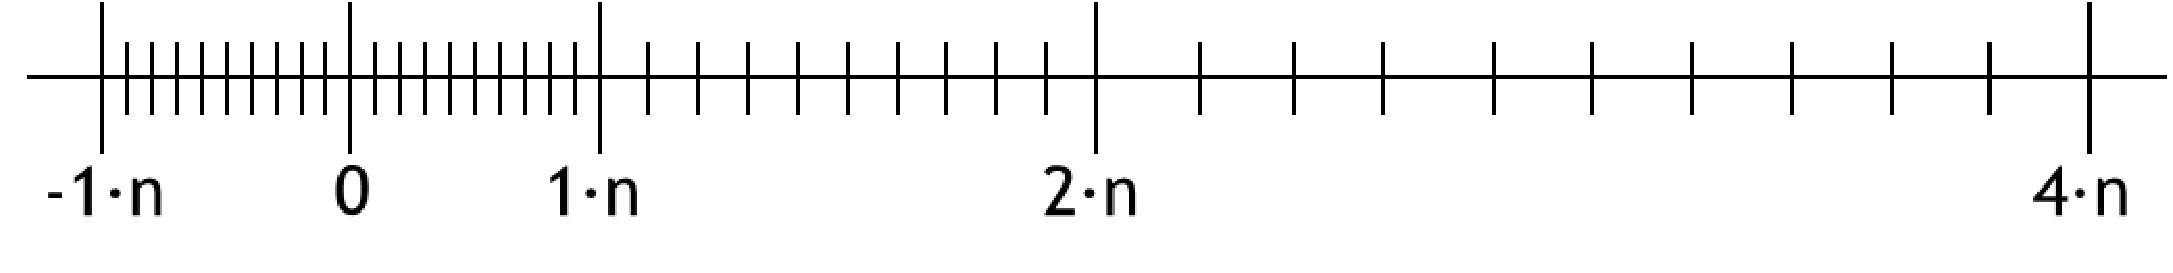
\includegraphics[width=10cm]{precision.pdf}
	\caption{Ilustraci�n del cambio de precisi�n con la magnitud de los n�meros representados.}
	\label{fig:precision}
\end{figure}

\subsection{Errores de desbordamiento}\index{Desbordamiento}
En el apartado anterior hemos visto una de las limitaciones de la representaci�n num�rica de los ordenadores; el hecho de usar una mantisa finita hace que solo unos pocos n�meros tengan representaci�n exacta, el resto hay que aproximarlos cometiendo errores de redondeo. En este apartado nos centraremos en estudiar las limitaciones debidas al hecho de usar un exponente finito; solo podemos representar un rango limitado de valores.
La figura \ref{fig:desbord} muestra esquem�ticamente el rango de n�meros representables. El n�mero negativo m�s peque�o representable, viene definido, por un bit de signo 1, para indicar que se trata de un n�mero negativo y la mantisa y el exponente m�s grandes que, dentro de las especificaciones del est�ndar, todav�a representan un n�mero finito. Cualquier n�mero negativo menor que �ste, produce un error de desbordamiento conocido en la literatura t�cnica con el nombre de \emph{overflow} negativo. El n�mero negativo m�s pr�ximo a cero, que se puede representar ser� aquel que tenga bit de signo 1, la mantisa (desnormalizada) m�s peque�a posible y el exponente m�s peque�o posible. Cualquier n�mero m�s pr�ximo a cero que este, ser� representado por el ordenador como cero. Se ha producido en este caso un error de desbordamiento conocido como \emph{underflow} negativo. 

De modo an�logo a como hemos definido el n�mero negativo m�s peque�o representable, podemos definir el n�mero positivo m�s grande representable. La �nica diferencia ser� que en este caso el bit de signo toma valor cero para indicar que es un  n�mero positivo. Cualquier n�mero mayor que �ste que queramos representar, provocar� un error de desbordamiento (\emph{overflow} positivo.) Por �ltimo, el n�mero positivo m�s pr�ximo a cero representable coincide con el correspondiente negativo, de nuevo salvo en el bit de signo, que ahora deber� ser cero. En el caso de tratar de representar un n�mero m�s peque�o el ordenador no lo distinguir� de cero, produci�ndose un desbordamiento denominado \emph{underflow} positivo. 
\begin{figure}[h]
	\centering
		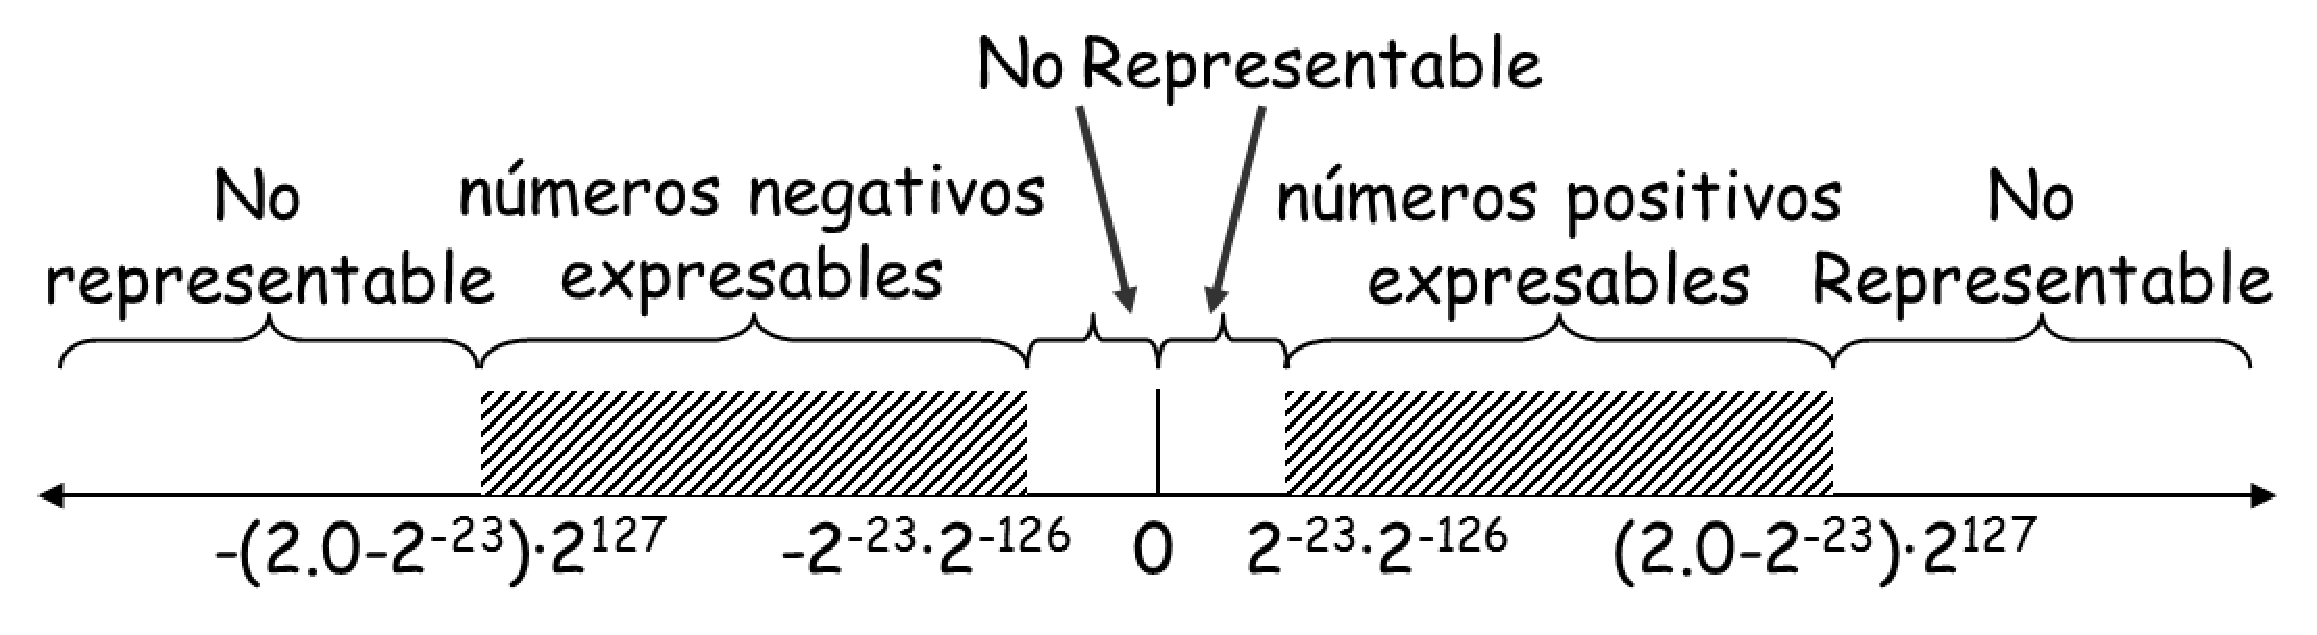
\includegraphics[width=10cm]{underandover.pdf}
	\caption{N�meros representables y desbordamientos en el est�ndar IEEE 754 de precisi�n simple.}	
	\label{fig:desbord}
\end{figure}

\section{Errores derivados de las operaciones aritm�ticas}\index{Errores aritm�ticos}
Hasta ahora, nos hemos centrado siempre en el problema de la representaci�n num�rica del computador. En esta secci�n vamos a introducir un nuevo tipo de errores que tienen si cabe todav�a m�s importancia desde el punto de vista del c�lculo cient�fico. Se trata de los errores derivados de las operaciones aritm�ticas.

Indirectamente ya se introdujo el problema en la secci�n anterior al hablar de la precisi�n del computador, y de la necesidad de igualar los exponentes de los sumandos al mayor de ellos antes de poder sumar en formato de punto flotante. Veamos en m�s detalle algunas consecuencias de la aritm�tica en punto flotante.
\subsection{Acumulaci�n de errores de redondeo}\index{Acumulaci�n de errores}

Para empezar, se ilustrar� el proceso de la suma de dos n�meros representados en base 10 en formato de punto flotante. Supongamos que queremos sumar los n�meros $99.99$ y $0.161$. Supongamos adem�s que seguimos una representaci�n en punto flotante con las siguientes limitaciones la mantisa es de cuatro d�gitos, el exponente es de dos d�gitos.

Si sumamos los n�meros, tal y como los hemos escrito m�s arriba, sin seguir formato de punto flotante, el resultado ser�a,

\begin{equation*}
99.99+0.161=100.151
\end{equation*}

Supongamos que los representamos ahora en el formato de punto flotante descrito m�s arriba, $99.99=9.999\times10^1$, $0.161=1.610\times10^{-1}$. Vamos a descomponer el proceso de sumar estos dos n�meros en cuatro pasos, que reflejan, esquem�ticamente, el proceso que seguir�a un computador.

\begin{enumerate}
\item \textbf{Alineamiento.} \index{Alineamiento}Consiste en representar el n�mero m�s peque�o empleando el exponente del mayor. Para ellos se desplazan hacia la derecha los d�gitos del n�mero m�s peque�o tantas posiciones como indique la diferencia de los exponentes de los dos n�meros y se cambiar el exponente del n�mero mas peque�o por el del m�s grande.
\begin{equation*}
1.610\times 10^{-1}\rightarrow 0.016\times10^1
\end{equation*}
Como cab�a esperar, el desplazamiento hacia la derecha de la mantisa produce la p�rdida de los �ltimos d�gitos del n�mero. Tenemos aqu� un primer error de redondeo en el proceso de alineamiento.

\item \textbf{Operaci�n.}
Una vez que los operandos est�n alineados, se puede realizar la operaci�n. Si la operaci�n es suma y los signos son iguales o si la operaci�n es resta y los signos son diferentes, se suman las mantisa. En otro caso se restan.

Es importante comprobar tras realizar la operaci�n si se ha producido desbordamiento de la mantisa; en el ejemplo propuesto:

\begin{tabular}{c r}
&$9.999\cdot10^1$\\
$+$&$0.016\cdot10^1$\\
\hline
&$10.015\cdot10^1$
\end{tabular}\\

No es posible emplear directamente el resultado de la suma de las mantisas de los sumandos como mantisa de la suma ya que requerir�a emplear un d�gito m�s. El resultado obtenido desborda el tama�o de la mantisa.

\item \textbf{Normalizaci�n.}
Si se ha producido desbordamiento de la mantisa, es preciso volver a normalizarla,
\begin{equation*}
10.015\times10^1=1.0015\times10^2
\end{equation*}
 
\item \textbf{Redondeo.} El desplazamiento de la mantisa hace que no quepan todo los d�gitos, por lo que es necesario redondearla (por truncamiento o por exceso),

\begin{equation*}
1.0015\times10^2=1.002\times10^2
\end{equation*}

Por �ltimo, se comprueba si las operaciones realizadas han producido desbordamiento del exponente, en cuyo caso el resultado ser�a un n�mero no representable: $\infty$ � $0$.

\item \textbf{Renormalizaci�n} Para n�meros en representaci�n binaria es preciso a veces volver a normalizar la mantisa despu�s del redondeo. Supongamos, como en el ejemplo anterior, una mantisa de cuatro bits, ---ahora con n�meros representados en binario--- y que tras realizar una operaci�n suma el resultado que se obtiene es $11.111\times2^1$. La mantisa ha desbordado y hay que normalizarla $11.111\times2^1\rightarrow1.1111\times2^2$. Tenemos que redondear la mantisa y lo normal en este caso dado que el n�mero estar�a exactamente en la mitad del intervalo entre dos n�meros representables, es hacerlo por exceso: $1.1111\times2^2\rightarrow10.000\times2^2$. la operaci�n de redondeo por exceso ha vuelto a desbordar la mantisa y, por tanto, hay que volver a normalizarla: $10.000\times2^2\rightarrow1.000\times2^3$.
\end{enumerate} 

Analicemos el error cometido para la suma empleada en los ejemplos anteriores. En aritm�tica exacta, el n�mero obtenido tras la suma es $100.152$. Empleando la representaci�n en punto flotante, con una mantisa de cuatro d�gitos el resultado es $1.002\times10^2=100.2$. por tanto, el error absoluto cometido es,
\begin{equation*}
\vert 100.151-100.2 \vert=0.049
\end{equation*}

y el error relativo,
\begin{equation*}
\left\vert\frac{100.151-100.2 }{100.152}\right\vert\approx 0.000489
\end{equation*}
En general puede comprobarse que para cualquier operaci�n aritm�tica b�sica $\odot \ $(suma, resta, multiplicaci�n divisi�n) y dos n�meros m�quina $x$, $y$ se cumple,

\begin{equation*}
\text{flotante}(x\odot y)=(x\odot y)\cdot(1+\delta) \ \ \vert \delta \vert \leq eps
\end{equation*}

Este enunciado se conoce como el axioma fundamental de la aritm�tica en punto flotante:\emph{ El eps del computador es la cota superior del error relativo en cualquier operaci�n aritm�tica b�sica realizada en punto flotante entre n�meros m�quina.} 

El axioma fundamental de la aritm�tica en punto flotante establece una cota superior para el error. En la pr�ctica, es frecuente que se encadenen un gran n�mero de operaciones aritm�ticas elementales. Al encadenar operaciones, los errores cometidos en cada una de ellas se acumulan.

Supongamos por ejemplo que queremos realizar la operaci�n $x\cdot(y+z)$ en aritm�tica flotante la operaci�n podr�amos describirla como,
\begin{align*}
\text{flotante}\left(x\cdot (y+z)\right)& =\left(x\cdot\text{flotante}(y+z)\right)\cdot(1+\delta_1)\\
 & = (x\cdot(y+z))\cdot(1+\delta_2)\cdot(1+\delta_1)\\
 & \approx (x\cdot(y+z))\cdot(1+2\delta)
\end{align*}

Donde $\delta_1$ representa el error relativo cometido en el producto y $\delta_2$ el error relativo cometido en la suma. Ambos errores est�n acotados por el \emph{eps} del ordenador ($\delta_1, \ \delta_2 \leq eps$). El valor $\delta$ se puede obtener como,
\begin{equation*}
(1+\delta_1)\cdot(1+\delta_2)=1+\delta_1\delta_2+\delta_1+\delta_2\approx 1+2\delta,\ \delta=\max(\delta_1,\delta_2)
\end{equation*}

Podemos concluir que, en este caso, el error de redondeo relativo duplica al de una operaci�n aritm�tica sencilla. En general, el error tender� a multiplicarse con el n�mero de operaciones aritm�ticas encadenadas.

Hay situaciones en las cuales los errores de redondeo que se producen durante una operaci�n aritm�tica son considerables por ejemplo, cuando se suman cantidades grandes con cantidades peque�as,

\begin{equation*}
\text{flotante}(1.5\cdot10^{38}+1.0\cdot10^0)=1.5\cdot10^{38} + 0
\end{equation*}

En este caso, durante el proceso de alineamiento, es preciso desplazar la mantisa del n�mero peque�o 38 posiciones decimales para poder sumarlo. Con cualquier mantisa que tenga menos de 38 d�gitos el resultado es equivalente a convertir el segundo sumando en cero.

Otro ejemplo es la p�rdida de la propiedad asociativa,

\begin{equation*}
\left. \begin{aligned}
x=1.5\cdot10^{38}\\
y=-1.5\cdot10^{38}\\
\end{aligned}
\right\}
\Rightarrow
(x+y)+1\neq x+(y+1)
\begin{cases}
(x+y)+1=1\\
x+(y+1)=0
\end{cases}
\end{equation*}

Los resultados pueden estar sometidos a errores muy grandes cuando la operaci�n aritm�tica es la sustracci�n de cantidades muy parecidas. Si, por ejemplo, queremos realizar la operaci�n $100.1-99.35=0.75$ y suponemos que estamos empleando una representaci�n en punto flotante con una mantisa de cuatro d�gitos y los n�meros representados en base 10 ($100.1=1.001\cdot10^2$, $99.35=9.935\cdot 10^1$) 

\begin{enumerate}
\item \textbf{Alineamiento}
\begin{equation*}
9.935\cdot 10^1\rightarrow 0.994 \cdot 10^2
\end{equation*}

\item \textbf{Operaci�n}

\begin{tabular}{c r}
&$1.001\cdot10^2$\\
$-$&$0.994\cdot10^2$\\
\hline
&$0.007\cdot10^2$
\end{tabular}\\

\item \textbf{normalizaci�n}
\begin{equation*}
0.007\cdot10^2\rightarrow 7.000\cdot10^{-1}
\end{equation*}
\end{enumerate}

Los pasos $4$ y $5$ no son necesarios en este ejemplo. Si calculamos ahora el error absoluto de redondeo cometido,
\begin{equation*}
\vert 0.75-0.7 \vert =0.05
\end{equation*} 

Y el error relativo,
\begin{equation*}
\left\vert\frac{0.75-0.7}{0.75}\right\vert\approx 0.0666
\end{equation*}
Es decir, se comete un error de un $6,7\%$. El problema en este caso surge porque en el proceso de alineamiento perdemos un d�gito significativo.

 En un sistema de representaci�n en punto flotante en que los n�meros se representan en base $\beta$ y el tama�o de la mantisa es $p$, Si las sustracciones se realizan empleando $p$ d�gitos, el error de redondeo relativo puede llegar a ser $\beta-1$.
 
Veamos un ejemplo para n�meros en base 10 ($\beta=10$). Supongamos que empleamos una mantisa de cuatro d�gitos y que queremos realizar la operaci�n $1.000\cdot10^0-9.999\cdot10^{-1}$. El resultado exacto ser�a, $1-0.9999=0.0001$. Sin embargo, en el proceso de alineamiento,
\begin{equation*}
9.999\cdot10^{-1}\rightarrow0.9999\cdot10^0
\end{equation*} 
Si redondeamos el n�mero por exceso, el resultado de la sustracci�n ser�a cero. Si lo redondeamos por defecto,

\begin{tabular}{c r}
&$1.000\cdot10^0$\\
$-$&$0.999\cdot10^0$\\
\hline
&$0.001\cdot10^0$
\end{tabular}\\

y el error relativo cometido ser�a,
\begin{equation*}
\left\vert\frac{1.000\cdot10^{-4}-1.000\cdot10^{-3}}{1.000\cdot10^{-4}}\right\vert=\frac{10^{-4}(10-1)}{10^{-4}}=10-1\Rightarrow\beta -1
\end{equation*}


Para paliar estos problemas, el est�ndar IEEE 754 establece que las operaciones aritm�ticas deben realizarse siempre empleando dos d�gitos extra para guardar los resultados intermedios. Estos dos d�gitos extra reciben el nombre de d�gitos de protecci�n o d�gitos de guarda (\emph{guard digits}).
Si repetimos la sustracci�n, $100.1-99.35$, empleando los dos d�gitos de guarda,

\begin{enumerate}
\item \textbf{Alineamiento}
\begin{equation*}
9.935{\color{red}00}\cdot=10^1\rightarrow 0.993{\color{red}50} \cdot 10^2
\end{equation*}

\item \textbf{Operaci�n}
\begin{tabular}{c r}
&$1.001{\color{red}00} \cdot10^2$\\
$-$&$0.993{\color{red}50}\cdot10^2$\\
\hline
&$0.007{\color{red}50}\cdot10^2$
\end{tabular}\\

\item \textbf{normalizaci�n}
\begin{equation*}
0.007{\color{red}50}\cdot10^2\rightarrow 7.500\cdot10^{-1}
\end{equation*}

\end{enumerate}
En este caso, obtenemos el resultado exacto. En general, empleando dos bits de guarda para realizar las sustracciones el error de redondeo es siempre menor que el \emph{eps} del computador.


\subsection{Anulaci�n catastr�fica}\index{Anulaci�n catastr�fica}
La anulaci�n catastr�fica se produce cuando en una operaci�n aritm�tica, t�picamente la sustracci�n,  los d�gitos m�s significativos de los operandos, que no est�n afectados por el redondeo, se cancelan entre s�. El resultado contendr� fundamentalmente d�gitos que s� est�n afectados por errores de redondeo. Veamos un ejemplo,

Supongamos que queremos realizar la operaci�n $b^2-4\cdot a \cdot c$ empleando n�meros en base 10, y una mantisa de 5 d�gitos. Supongamos que los n�meros empleados son: $b= 3.3357\cdot10^0$, $a=1.2200\cdot10^0$, $c=2.2800\cdot10^0$. El resultado exacto de la operaci�n es,
\begin{equation}
b^2-4\cdot a\cdot c=4.944\cdot10^{-4}
\end{equation}

Si realizamos las operaciones en la representaci�n pedida,
\begin{align*}
b^2=1.1126{\color{red}89}\cdot10^1\\
4\cdot a\cdot c=1.1126{\color{red}40}\cdot10^1\\
b^2-4\cdot a\cdot c=5.0000\cdot10^{-4}
\end{align*}

El error relativo cometido es aproximadamente un 1\%. Como se han utilizado dos bits de guarda en las operaciones intermedias, la sustracci�n no comente en este caso error alguno. El error se debe a los redondeos de los resultados anteriores. Una vez realizada la sustracci�n, el resultado solo contiene los d�gitos sometidos a redondeo ya que los anteriores se han anulado en la operaci�n.

Como regla pr�ctica se debe evitar al realizar operaciones aritm�ticas aquellas situaciones en las que se sustraen cantidades casi iguales. Veamos otro ejemplo, para ilustrar esta idea. Supongamos que queremos realizar la operaci�n,
\begin{equation*}
y=\sqrt{x^2+1}-1
\end{equation*}
Para valores peque�os de $x$, esta operaci�n implica una anulaci�n con p�rdida de d�gitos significativos. Una posible soluci�n es utilizar una forma alternativa de construir la ecuaci�n. Si multiplicamos y dividimos por el conjugado,

\begin{equation*}
y=(\sqrt{x^2+1}-1)\cdot\left(\frac{\sqrt{x^2+1}+1}{\sqrt{x^2+1}+1}\right)=\frac{x^2}{\sqrt{x^2+1}+1}
\end{equation*}

\subsection{Errores de desbordamiento}

Al, hablar del rango finito de los n�meros representables, se indic� c�mo trata el �standar IEEE 754 los n�meros que desbordan los l�mites de representaci�n. Al realizar operaciones aritm�ticas, es posibles llegar a situaciones en las que el resultado sea un n�mero no representable bien por se demasiado grande en magnitud, (\emph{Overflow} positivo o negativo) o por ser demasiado peque�o, (\emph{underflow} positivo o negativo.) Un ejemplo que nos permite ilustrar este fen�meno es el del c�lculo del m�dulo de un vector,

\begin{equation*}
\vert\vert\vec{v}\vert\vert=\vert\vert(v_1, v_2\cdots v_n\vert\vert=\sqrt{\sum_{i=1}^nv_i^2}
\end{equation*}

Supongamos que creamos el siguiente programa en Matlab para calcular el m�dulo de un vector

\begin{lstlisting}
function m=norma(x)
%inicializamos a cero la variable que contendr� la norma del vector.
m=0;
n=length(x) %calculamos la longitud del vector.
%creamos un bucle para ir sumando los cuadrados de las componentes
for i=1:n
m=m+x(i)^2;
end

%calculamos la ra�z cuadrada del resultado del bucle
m=sqrt(m)
\end{lstlisting}

El programa anterior provocar� un error de desbordamiento incluso para n=1, si introducimos un n�mero cuyo cuadrado sea mayor que el mayor n�mero representable. Por ejemplo si introducimos el n�mero, $ 2^{1024/2}=1.340780792994260e+154$ en nuestro programa Matlab devolver� como soluci�n \emph{inf}. Es decir, el resultado produce un error de desbordamiento. El problema se produce en el bucle, al calcular el cuadrado del n�mero,
\begin{equation*}
\left(2^{1024/2}\right)^2=2^{1024}> (2-2^{-52})\cdot 2^{1023}
\end{equation*}

Una vez producido el desbordamiento el resto de las operaciones quedan invalidadas. Como en casos anteriores, la soluci�n a este tipo de problemas exige modificar la forma en que se realizan los c�lculos. Un primer paso ser�a igualar el m�dulo al valor absoluto del n�mero cuando n=1. De este modo, el modulo del n�mero propuesto en el ejemplo anterior se podr�a calcular correctamente.

Todav�a es posible mejorar el programa, y ampliar el rango de vectores para los que es posible calcular el m�dulo. Para ello es suficiente recurrir a un peque�o artificio: dividir los elementos del vector por el elemento de mayor tama�o en valor absoluto, calcular el m�dulo del vector resultante, y multiplicar el resultado de nuevo por el elemento de mayor tama�o,
\begin{align*}
\sqrt{\sum_{i=1}^nv_i^2}=\vert\max{v_i}\vert\cdot\sqrt{\sum_{i=1}^n\left(\frac{v_i}{\vert\max{v_i}\vert}\right)^2}
\end{align*}

El siguiente c�digo permite calcular el m�dulo de un vector usando este procedimiento\footnote{El programa no funcionar� correctamente para vectores cuyos primeros elementos sean 0, $(0,0,0\cdots$},

\begin{lstlisting}
function m=norma(x)
n=length(x); %calculamos la longitud del vector.
%si n=1 nos limitamos a devolver el valor absoluto del n�mero introducido
if n==1
	x=abs(x);
else
% inicializamos con el primer elemento la variable que contendr�
% al mayor de los elementos del vector
mayor=abs(x(1));

% inicialimos a 1 la variable que contendr� la suma de
% los cuadrados de los elementos divididos por el valor de ello

nscalado=1

% creamos un bucle para ir sumando los cuadrados de las componentes.
% empezamos en el segundo elemento, puesto que el primero ya lo tenemos.
	for i=2:n	
		% calculamos el valor absoluto del elemento i
		modxi=abs(x(i))
		% comparamos con modxi con el mayor elemento obtenido hasta
		% aqu�
		if mayor<modxi
			% si modxi es mayor, ser� el elemento m�s grande encontrado
			% hasta esta iteraci�n
			% cambiamos el valor de la suma 
			mscalado=1+mscalado*(modxi/mayor)^2;
			% definimos mayor como el nuevo valor encontrado
			mayor=modxi;
		else
			% si no es el m�s grande, nos limitamos a sumarlo al resto
			mscalado=mscalado+(modxi/mayor)^2;
	
		end
% una vez completado el bucle que calcula la suma de cuadrados,
% obtenemos la ra�z cuadrada, y multiplicamos por el mayor.
m=mayor*sqrt(mscalado)
\end{lstlisting}

Si aplicamos este programa a obtener la norma del vector,
\begin{equation*}
x=[2^{1024/2}\ 2^{1024/2}]
\end{equation*}
obtenemos como resultado,
\begin{equation*}
m=1.896150381621836\cdot10^{154}
\end{equation*}
En lugar de un error de desbordamiento (\emph{inf}).



  	 
\chapter{C�lculo de ra�ces de una funci�n}

\section{Ra�ces de una funci�n}
Se entiende por ra�ces de una funci�n real $f(x):\mathbb{R} \rightarrow \mathbb{R}$. los valores $x=r$ que satisfacen, $f(r)=0$

El c�lculo de las ra�ces de una funci�n, tiene una gran importancia en la ciencia, donde un n�mero significativo de problemas pueden reducirse a obtener la ra�z o ra�ces de una ecuaci�n.

La obtenci�n de la ra�z de una ecuaci�n es inmediata en aquellos casos en que se conoce la forma anal�tica de su funci�n inversa $f^{-1}$, ($f(x)=y\Rightarrow f^{-1}(y)=x$). En este caso, $r=f^{-1}(0)$. Por ejemplo,
\begin{align*}
f(x)&=x^2-4\\
f^{-1}(y)&=\pm\sqrt{y+4}\Rightarrow r=f^{-1}(0)=\pm 2\
\end{align*}

Sin embargo, en muchos casos de inter�s las funciones no pueden invertirse.  Un ejemplo, extra�do de la f�sica es la ecuaci�n de Kepler para el c�lculo de las �rbitas planetarias,
\begin{equation*}
x-a\sin(x)=b
\end{equation*}

Donde $a$ y $b$ son par�metros conocidos y se desea conocer el valor de $x$. La soluci�n de la ecuaci�n de Kepler es equivalente a obtener las ra�ces de la funci�n $f(x)=x-a\sin(x)-b$. (La figura \ref{fig:kepler} muestra un ejemplo de dicha funci�n.) En este caso, no se conoce la funci�n inversa, y solo es posible conocer el valor de la ra�z, aproximadamente, empleando m�todos num�ricos.
\begin{figure}[h]
\centering
		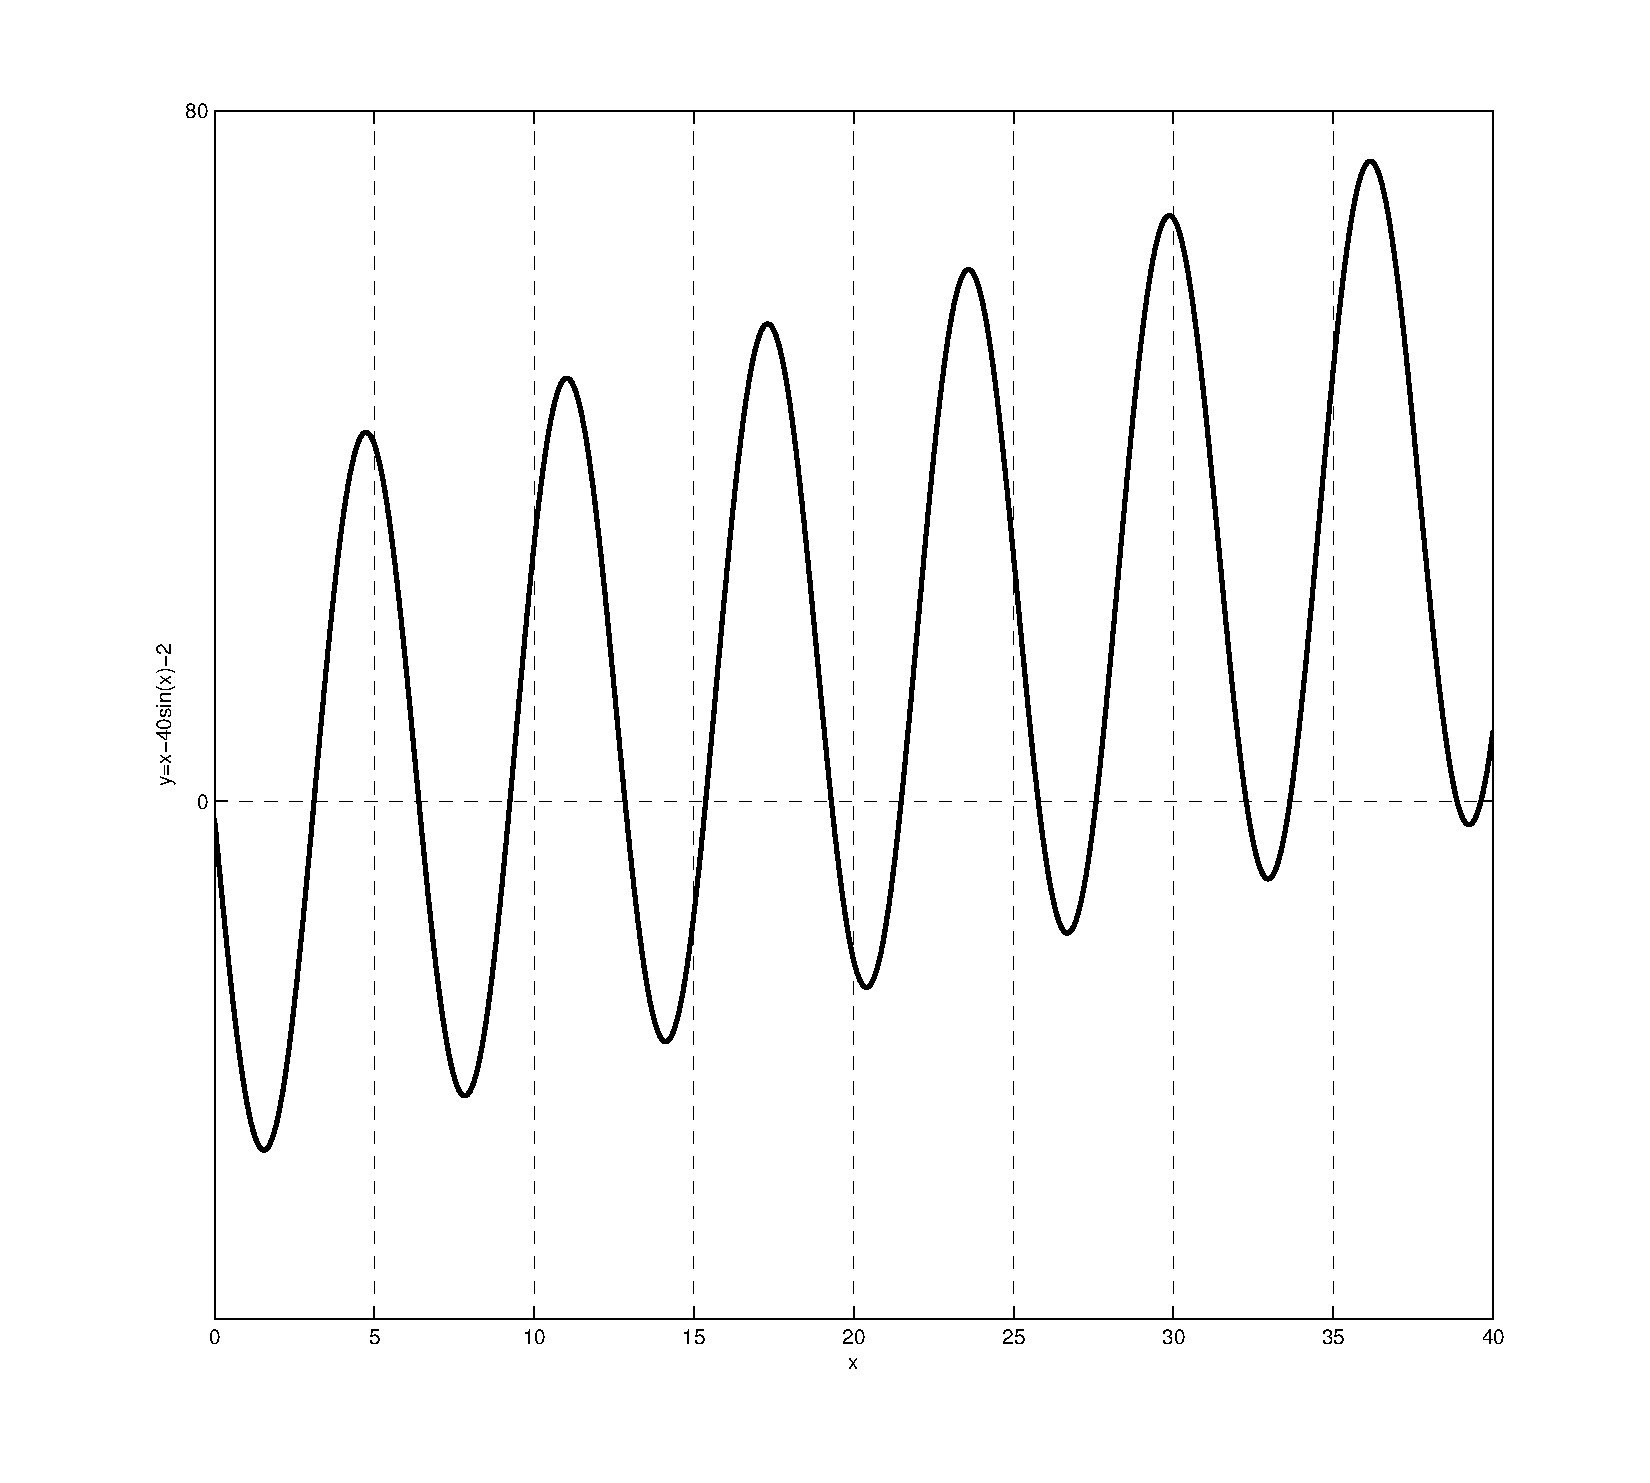
\includegraphics[width=12cm]{kepler.pdf}
	\caption{Ejemplo de ecuaci�n de Kepler para $a=40$ y $b=2$}
	\label{fig:kepler}
\end{figure}

\paragraph*{M�todos iterativos}Todos los m�todos que se describen en este cap�tulo, se basan en procedimientos iterativos. La idea es estimar un valor inicial para la ra�z $r_0$, y a partir de �l ir refinando paso a paso la soluci�n, de modo que el resultado se acerque cada vez m�s al valor real de la ra�z. Cada nueva aproximaci�n a la ra�z se obtiene a partir de las aproximaciones anteriores. 
\begin{align*}
r_0\ \ \  \rightarrow \  \ r_1  \ \ \rightarrow \ \ r_2 \ \ \rightarrow \cdots \rightarrow \ \ r_k \ \rightarrow \cdots\\
\vert f(r_0)\vert \ge \vert f(r_1)\vert \ge \vert f(r_2)\vert \ge \cdots \ge \vert f(r_k)\vert \ge \cdots
\end{align*}

El proceso que lleva de una soluci�n aproximada a la siguiente se conoce con el nombre de \emph{iteraci�n}. Lo habitual es que en cada iteraci�n se realicen las mismas operaciones matem�ticas una y otra vez. 

El proceso se detiene cuando la soluci�n alcanzada se estima lo suficientemente pr�xima a la soluci�n real como para darla por buena. Para ello, se suele establecer un valor (\emph{tolerancia}) que act�a como criterio de convergencia. De este modo, las iteraciones se repiten hasta que se llega a un valor $r_n$ 	que cumple,
\begin{equation*}
\vert f(r_n) \vert \leq \text(tol)
\end{equation*}

Se dice entonces que el algoritmo empleado para obtener la ra�z ha convergido en \emph{n} iteraciones. Por otro lado, es importante se�alar que los algoritmos para el c�lculo de ra�ces de una funci�n no siempre convergen. Hay veces en que no es posible aproximarse cada vez m�s al valor de la ra�z bien por la naturaleza de la funci�n o bien por que el algoritmo no es adecuado para obtenerla.

\paragraph*{B�squeda local.} Una funci�n puede tener cualquier n�mero de ra�ces, incluso infinitas, basta pensar por ejemplo en funciones trigonom�tricas como $\cos(x)$. Una caracter�stica importante de los m�todos descritos en este cap�tulo es que solo son capaces de aproximar una ra�z. La ra�z de la funci�n a la que el m�todo converge depende de el valor inicial $r_0$ con el que se comienza la b�squeda iterativa\footnote{En ocasiones, como veremos m�s adelante no se suministra al algoritmo un valor inicial, sino un intervalo en el que buscar la ra�z}. Por ello reciben el nombre de m�todos locales. Si queremos encontrar varias (o todas) las ra�ces de una determinada funci�n, es preciso emplear el m�todo para cada una de las ra�ces por separado, cambiando cada vez el punto de partida.

\section{Metodos iterativos locales}
\subsection{M�todo de la bisecci�n}
\paragraph*{Teorema de Bolzano.}
\begin{quote}
Si una funcion $f(x)$, continua en el intervalo $[a, b]$, cambia de signo en los extremos del intervalo: $f(a)\cdot f(b) \le 0$, debe tener una ra�z en el intervalo [a, b]. (figura: \ref{fig:bolzano}) 
\end{quote}

\begin{figure}[h]
\centering
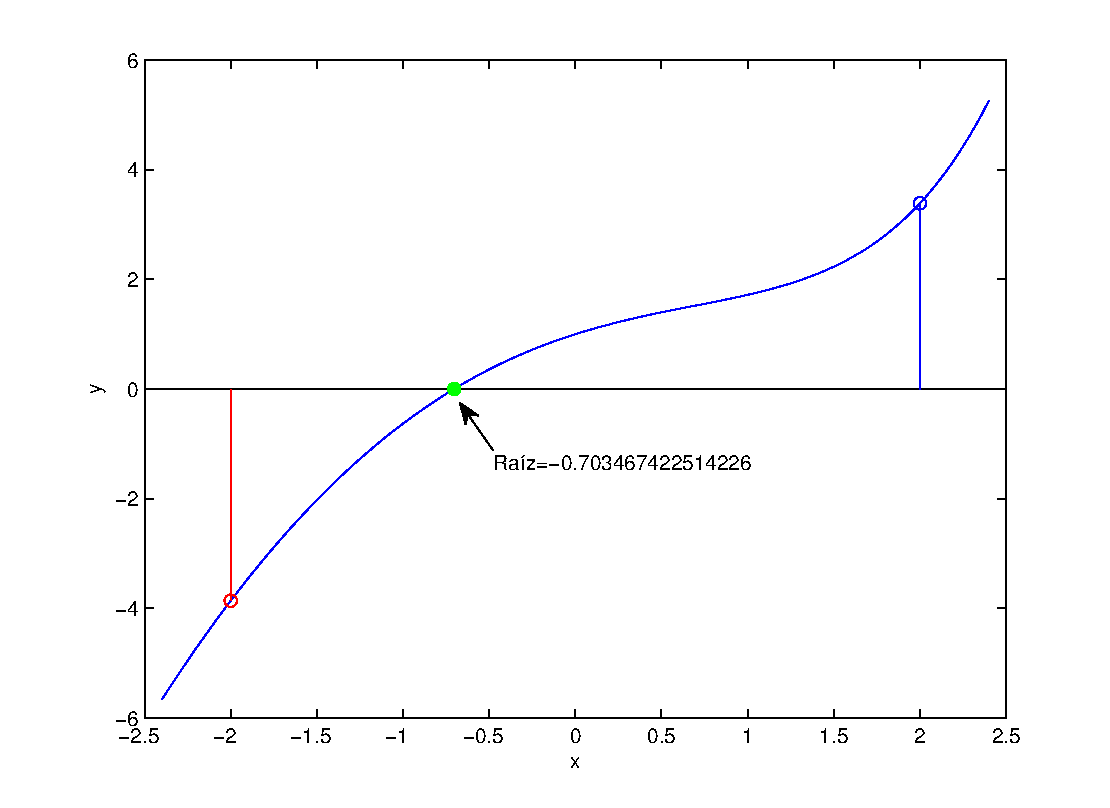
\includegraphics[width=14cm]{bolzano.pdf}
\caption{Ilustraci�n del teorema de Bolzano}
\label{fig:bolzano}
\end{figure}

El conocido teorema de Bolzano, suministra el m�todo m�s sencillo de aproximar la ra�z de una funci�n: Se parte de un intervalo inicial en el que se cumpla el teorema; y se va acotando sucesivamente el intervalo que contiene la ra�z, reduci�ndolo a la mitad en cada iteraci�n, de forma que en cada nuevo intervalo se cumpla siempre el teorema de Bolzano.

\begin{figure}[h]
\centering
\begin{tikzpicture}
%\usetikzlibrary{shapes.geometric}
\path (5,0) node(a) [rectangle,draw=blue, very thick,align=center,rounded corners]{Partimos de $[a,b]$\\ con\\ $f(a)\cdot f(b)<0$}
(5,-2) node(b)[rectangle,draw=blue, thick,rounded corners]{Calculamos $c=\frac{a+b}{2}, f(c)$}
(5,-4) node(c)[diamond,aspect=3,draw=red,thick]{es $\vert f(c) \vert \le \text{tol}$?}
(9,-4) node(d)[rectangle,draw=blue,align=center,very thick, rounded corners]{convergencia:\\ terminar}
(5,-6) node(e)[diamond,aspect=3,draw=red,thick]{es $f(a)\cdot f(c) < 0$?}
(9.5,-6) node(f)[rectangle,draw=blue,thick,rounded corners,align=center]{$b=c$\\$f(b)=f(c)$}
(5,-8) node(g)[rectangle,draw=blue,thick,rounded corners,align=center]{$a=c$\\$f(a)=f(c)$};
\draw[blue,-latex](a.south)--(b);
\draw[blue,-latex](b.south)--(c);
\draw[blue,-latex](c.east)--(d);
\draw (7.5,-4)node[above]{S�};
\draw[blue,-latex](c.south)--(e);
\draw (5,-5)node[right]{No};
\draw[blue,-latex](e.east)--(f);
\draw (8,-6)node[above]{S�};
\draw[blue,-latex](e.south)--(g);
\draw (5,-7.2)node[right]{No};
\draw[blue,-latex](g.south)|-(2,-9)|-(b);
\draw[blue,-latex](f.east)-|(11,-2)--(b);
\end{tikzpicture}
\caption{Diagrama de flujo del m�todo de la bisecci�n}
\label{fig:dfbisec}
\end{figure}
En la figura \ref{fig:dfbisec} se muestra un diagrama de flujo correspondiente al m�todo de la bisecci�n. El punto de partida es un intervalo $[a,b]$ en el que se cumple el teorema de Bolzano, y que contiene por tanto al menos una ra�z. Es interesante hacer notar que el teorema de Bolzano se cumple siempre que la funci�n sea continua en el intervalo $[a,b]$ y existan un n�mero impar de ra�ces. Por esto es importante realizar cuidadosamente la elecci�n del intervalo $[a,b]$, si hay m�s de una ra�z, el algoritmo puede no converger.

 Una vez que se tiene el intervalo se calcula el punto medio $c$. A continuaci�n se compara el valor que toma la funci�n en $c$, es decir $f(c)$ con la tolerancia. Si el valor es menor que �sta, el algoritmo ha encontrado un valor aproximado de la ra�z con la tolerancia requerida, con lo que $c$ es la ra�z y no hace falta seguir buscando. Si por el contrario, $f(c)$ est� por encima de la tolerancia requerida, comparamos su signo con el que toma la funci�n en uno cualquiera de los extremos del intervalo, En el diagrama de flujo se ha elegido el extremo $a$, pero el algoritmo funcionar�a igualmente si eligi�ramos $b$. Si el signo de $f(c)$ coincide con el que toma la funci�n en el extremo del intervalo elegido, $c$ sustituye al extremo, (hacemos $a=c$ y $f(a)=f(c)$) si por el contrario el signo es distinto, hacemos que $c$ sustituya al otro extremo del intervalo. (hacemos $b=c$ y $f(b)=f(c)$). Este proceso se repetir� hasta que se cumpla que $f(c)\le \text{tol}$ 

El proceso se muestra gr�ficamente en la figura \ref{fig:bisec}, para un caso particular. Se trata de obtener la ra�z de la funci�n mostrada en la figura \ref{fig:bolzano}, $f(x)=e^x-x^2$. esta funci�n tiene una �nica ra�z: $r\approx -0.0735$. Para iniciar el algoritmo se ha elegido un intervalo $[a=-2,b=2]$. La figura \ref{fig:bisec}, muestra tres iteraciones sucesivas,y la soluci�n final, que se obtiene al cabo de ocho iteraciones en �ste ejemplo, para el que se a empleado una tolerancia $tol=0.01$. En la secuencia de gr�ficas se puede observar tambi�n la evoluci�n del intervalo de b�squeda, $[-2, 2]\rightarrow [-2, 0] \rightarrow [-1, 0] \rightarrow [-1, -0.5] \cdots$; as� como el cambio alternativo del l�mite derecho o izquierdo, para asegurar que la ra�z queda siempre dentro de los sucesivos intervalos de b�squeda obtenidos. 
\begin{figure}
\centering
\subfigure[intervalo inicial]{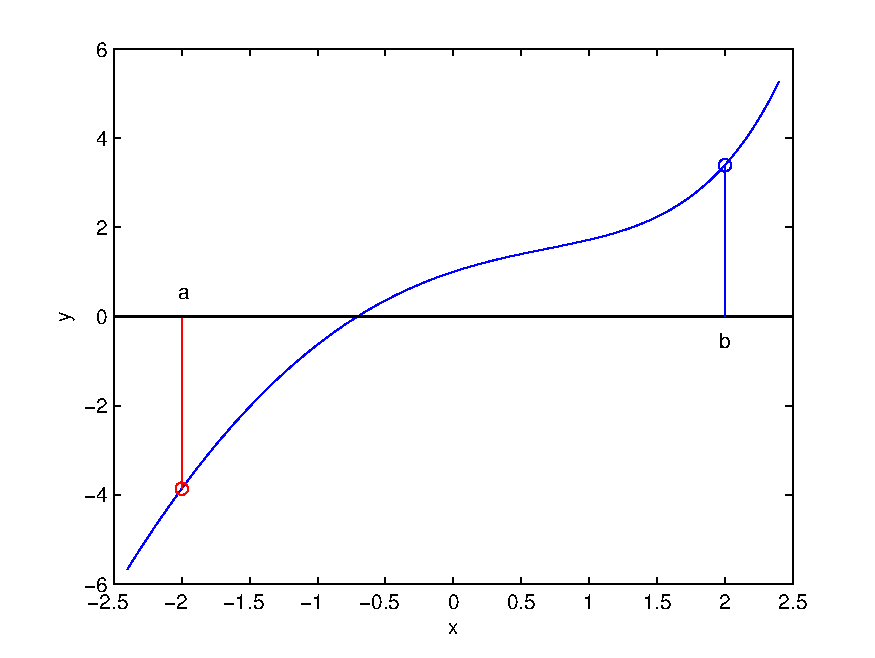
\includegraphics[width=7cm]{rint0.pdf}} \qquad
\subfigure[iteracion 1]{\includegraphics[width=7cm]{rint1.pdf}}\\
\subfigure[iteracion 2]{\includegraphics[width=7cm]{rint2.pdf}}\qquad
\subfigure[iteracion 3]{\includegraphics[width=7cm]{rint3.pdf}}\\
\subfigure[iteracion 6: ra�z alcanzada]{\includegraphics[width=7cm]{rint4.pdf}}

\caption{proceso de obtenci�n de la ra�z de una funci�n por el m�todo de la bisecci�n }
\label{fig:bisec}
\end{figure}

\subsection{M�todo de interpolaci�n lineal o (\emph{Regula falsi})}
Este m�todo supone una mejora del anterior ya que, en general,  converge m�s r�pidamente. La idea es modificar el modo en que calculamos el punto $c$. En el caso del m�todo de la bisecci�n el criterio consist�a en ir tomando en cada iteraci�n el punto medio del intervalo que contiene la ra�z. El m�todo de interpolaci�n lineal, elige como punto $c$ el punto de corte con el eje x, de la recta que pasa por los puntos $\left(a,f(a)\right)$ y $\left(b,f(b)\right)$. Es decir la recta que corta a la funci�n $f(x)$ en ambos l�mites del intevalo que contiene a la ra�z buscada. La recta que pasa por ambos puntos puede construirse a partir de ellos como,
\begin{equation*}
y=\frac{f(a)-f(b)}{a-b}\cdot(x-b)+f(b)
\end{equation*}
el punto de corte con el eje $x$, que ser� el valor que tomaremos para $c$, se obtiene cuando $y=0$,
\begin{equation*}
0=\frac{f(a)-f(b)}{a-b}\cdot(x-b)+f(b)
\end{equation*}

y despejando $c\equiv x$ en la ecuaci�n anterior obtenemos,
\begin{equation*}
c=b-\frac{f(b)}{f(b)-f(a)}\cdot(b-a)
\end{equation*}

La figura \ref{fig:regulaf} muestra  gr�ficamente la posici�n del punto $c$ obtenido mediante el m�todo de interpolaci�n. 

\begin{figure}[h]
\centering
\includegraphics[width=14cm]{rinter00.pdf}

\caption{Obtenci�n de la recta que une los extremos de un intervalo $[a,b]$  que contiene una ra�z de la funci�n}
\label{fig:regulaf}
\end{figure}

Por lo dem�s, el procedimiento es el mismo que en el caso del m�todo de la bisecci�n. Se empieza con un intervalo $[a,b]$ que  contenga una ra�z, se obtiene el punto $c$ por el procedimiento descrito y se intercambia $c$ con el extremo del intervalo cuya imagen $f(a)$ o $f(b)$ tenga el mismo signo que $f(c)$ el procedimiento se repite iterativamente hasta que f(c) sea menor que el valor de tolerancia preestablecido. 

\begin{figure}[h]
\centering
\begin{tikzpicture}
%\usetikzlibrary{shapes.geometric}
\path (5,0) node(a) [rectangle,draw=blue, very thick,align=center,rounded corners]{Partimos de $[a,b]$\\ con\\ $f(a)\cdot f(b)<0$}
(5,-2) node(b)[rectangle,draw=blue, thick,rounded corners,align=center]{Calculamos\\ $c=b-\frac{f(b)}{f(b)-f(a)}\cdot(b-a), f(c)$}
(5,-4) node(c)[diamond,aspect=3,draw=red,thick]{es $\vert f(c) \vert \le \text{tol}$?}
(9,-4) node(d)[rectangle,draw=blue,align=center,very thick, rounded corners]{convergencia:\\ terminar}
(5,-6) node(e)[diamond,aspect=3,draw=red,thick]{es $f(a)\cdot f(c) < 0$?}
(9.5,-6) node(f)[rectangle,draw=blue,thick,rounded corners,align=center]{$b=c$\\$f(b)=f(c)$}
(5,-8) node(g)[rectangle,draw=blue,thick,rounded corners,align=center]{$a=c$\\$f(a)=f(c)$};
\draw[blue,-latex](a.south)--(b);
\draw[blue,-latex](b.south)--(c);
\draw[blue,-latex](c.east)--(d);
\draw (7.5,-4)node[above]{S�};
\draw[blue,-latex](c.south)--(e);
\draw (5,-5)node[right]{No};
\draw[blue,-latex](e.east)--(f);
\draw (8,-6)node[above]{S�};
\draw[blue,-latex](e.south)--(g);
\draw (5,-7.2)node[right]{No};
\draw[blue,-latex](g.south)|-(2,-9)|-(b);
\draw[blue,-latex](f.east)-|(11,-2)--(b);
\end{tikzpicture}
\caption{Diagrama de flujo del m�todo de interpolaci�n lineal}
\label{fig:regula}
\end{figure}

En la figura \ref{fig:regula} se muestra el diagrama de flujo para el m�todo de interpolaci�n lineal. Como puede verse, es id�ntico al de la bisecci�n excepto en el paso en que se obtiene el valor de $c$, donde se ha sustituido el c�lculo del punto medio del intervalo de b�squeda, por el c�lculo del punto de corte con el eje de abscisas  de la recta que une los extremos del intervalo.

La figura \ref{fig:iterr2} Muestra gr�ficamente el proceso iterativo seguido para obtener la ra�z de una funci�n en un intervalo mediante el m�todo de interpolaci�n lineal. Se ha empleado la misma funci�n y el mismo intervalo inicial que en el caso de la bisecci�n. 

Es f�cil ver, sin embargo, que los puntos intermedios que obtiene el algoritmo hasta converger a la ra�z son distintos. De hecho, el algoritmo emplea ahora tan solo siete iteraciones para obtener la ra�z, empleando el mismo valor para la tolerancia, 0.01, que se emple� en el m�todo de la bisecci�n.

Una observaci�n final, se ha dicho al principio que �ste m�todo supone una mejora al m�todo anterior de la bisecci�n. Esto no siempre es cierto. El m�todo de la bisecci�n tiene una tasa de convergencia constante, cada iteraci�n divide el espacio de b�squeda por la mitad. Sin embargo la convergencia del m�todo de interpolaci�n  lineal depende de la funci�n $f(x)$ y de la posici�n relativa de los puntos iniciales $(a, f(a))$  y $(b, f(b))$ con respecto al la ra�z. Por esto no es siempre cierto que converja m�s r�pido que el m�todo de  la bisecci�n. Por otro lado, el c�lculo de los sucesivos valores del punto $c$, requiere m�s operaciones aritm�ticas en el m�todo de interpolaci�n, con lo que cada iteraci�n resulta m�s lenta que en el caso de la bisecci�n.
\begin{figure}
\centering
\subfigure[intervalo inicial]{\includegraphics[width=7cm]{rinter0.pdf}} \qquad
\subfigure[iteracion 1]{\includegraphics[width=7cm]{rinter1.pdf}}\\
\subfigure[iteracion 2]{\includegraphics[width=7cm]{rinter2.pdf}}\qquad
\subfigure[iteracion 3]{\includegraphics[width=7cm]{rinter3.pdf}}\\
\subfigure[iteracion 6: ra�z alcanzada]{\includegraphics[width=7cm]{rinter4.pdf}}

\caption{Proceso de obtenci�n de la ra�z de una funci�n por el m�todo de interpolaci�n lineal}
\label{fig:iterr2}
\end{figure}

\subsection{M�todo de Newton-Raphson}
El m�todo de Newton se basa en la expansi�n de una funci�n $f(x)$ en serie de Taylor en el entorno de un punto $x_0$,
\begin{equation*}
f(x)\approx f(x_0)+f'(x_0)(x-x_0)+\frac{1}{2}f''(x_0)(x-x_0)^2+\cdots+\frac{1}{n!}f^{(n)}(x_0)(x-x_0)^n+\cdots
\end{equation*}
 Pertenece a una familia de m�todos ampliamente empleados en c�lculo num�rico. La idea en el caso del m�todo de Newton es aproximar la funci�n para la que se desea obtener la ra�z, mediante el primer t�rmino de la serie de Taylor. Es decir aproximar localmente $f(x)$, en el entorno de $x_0$ por la recta,
\begin{equation*}
 f(x_0)+f'(x_0)(x-x_0)
\end{equation*}
Esta recta, es precisamente la recta tangente a la curva $f(x)$ en el punto $x_0$ (figura \ref{fig:newton1})
\begin{figure}[h]
\centering
\includegraphics[width=14cm]{newt0.pdf}[h]
\caption{Recta tangente a la funci�n $f(x)$ en el punto $x_0$}
\label{fig:newton1}
\end{figure}

El m�todo consiste en obtener el corte de esta recta tangente con el eje de abscisas,
\begin{equation*}
0= f(x_0)+f'(x_0)(x-x_0)
\end{equation*}

y despejando x,

\begin{equation*}
x=x_0-\frac{f(x_0)}{f'(x_0)}
\end{equation*}

A continuaci�n se eval�a la funci�n en el punto obtenido $x\rightarrow f(x)$. Como en los m�todos anteriores, se compara el valor de $f(x)$ con una cierta tolerancia preestablecida. Si es menor, el valor de $x$ se toma como ra�z de la funci�n. Si no, se vuelve aplicar el algoritmo, empleando ahora el valor de x que acabamos de obtener como punto de partida. Cada c�lculo constituye una nueva iteraci�n y los sucesivos valores obtenidos para $x$, convergen a la ra�z,

\begin{equation*}
x_0\rightarrow x_1=x_0-\frac{f(x_0)}{f'(x_0)}\rightarrow x_2=x_1-\frac{f(x_1)}{f'(x_1)}\rightarrow  \cdots \rightarrow x_n=x_{n-1}-\frac{f(x_{n-1})}{f'(x_{n-1})}\rightarrow \cdots
\end{equation*}

La figura \ref{fig:newton} muestra un diagrama de flujo correspondiente al m�todo de Newton. Si se compara con los diagramas de flujo de los algoritmos anteriores, el algoritmo de Newton resulta algo m�s simple de implementar. Sin embargo es preciso evaluar en cada iteraci�n el valor de la funci�n y el de su derivada. 

El c�lculo de la derivada, es el punto d�bil de este algoritmo, ya que para valores $x_0$ pr�ximos a un m�nimo o m�ximo local obtendremos valores de la derivada pr�ximos a cero, lo que puede causar un error de desbordamiento al calcular el punto de corte de la recta tangente con el eje de abscisas o hacer que el algoritmo converja a una ra�z alejada del punto inicial de b�squeda.
 
\begin{figure}[h]
\centering
\begin{tikzpicture}
%\usetikzlibrary{shapes.geometric}
\path (5,0) node(a) [rectangle,draw=blue, very thick,align=center,rounded corners]{Partimos de un punto inicial $x_0$}
(5,-2) node(b)[rectangle,draw=blue, thick,rounded corners,align=center]{Calculamos\\ $x=x_0-\frac{f(x_0)}{f'(x_0)}, f(x)$}
(5,-4) node(c)[diamond,aspect=3,draw=red,thick]{es $\vert f(x) \vert \le \text{tol}$?}
(9,-4) node(d)[rectangle,draw=blue,align=center,very thick, rounded corners]{convergencia:\\ terminar}
(5,-6) node(g)[rectangle,draw=blue,thick,rounded corners,align=center]{$x_0=x$};
\draw[blue,-latex](a.south)--(b);
\draw[blue,-latex](b.south)--(c);
\draw[blue,-latex](c.east)--(d);
\draw (7.5,-4)node[above]{S�};
\draw[blue,-latex](c.south)--(g);
\draw (5,-5)node[right]{No};
\draw[blue,-latex](g.south)|-(2,-7)|-(b);

\end{tikzpicture}
\caption{Diagrama de flujo del m�todo de Newton-Raphson}
\label{fig:newton}
\end{figure}

La figura \ref{fig:newton2} muestra un ejemplo de obtenci�n de la ra�z de una funci�n mediante el m�todo de Newton. El m�todo es m�s r�pido que los dos anteriores, es decir, partiendo de una distancia comparable a la ra�z, es el que converge en menos iteraciones. 

En el ejemplo de la figura se ha obtenido la ra�z para la misma funci�n que en los ejemplos del m�todo de la bisecci�n e interpolaci�n lineal. Se ha empezado sin embargo en un punto m�s alejado de la ra�z, para que pueda observarse mejor en la figura la evoluci�n del algoritmo. En cada uno de los gr�ficos que componen la figura pueden observarse  los pasos del algoritmo: dado el punto  $x_i$, se calcula  la recta tangente a la funci�n $f(x)$ en el punto y se obtiene un nuevo punto $x_{i+1}$,  como el corte de dicha recta tangente con el eje de abscisas.

En este ejemplo el algoritmo converge en las cinco iteraciones que se muestran en la figura, para la misma tolerancia empleada en los m�todos anteriores, $tol=0.01$. El punto de inicio empleado fue $x_0=2.5$, por tanto esta fuera del intervalo $[-2, 2]$ y m�s alejado de la ra�z que en el caso de los m�todos anteriores.   

\begin{figure}
\centering
\subfigure[intervalo inicial]{\includegraphics[width=7cm]{newt01.pdf}} \qquad
\subfigure[iteracion 1]{\includegraphics[width=7cm]{newt02.pdf}}\\
\subfigure[iteracion 2]{\includegraphics[width=7cm]{newt1.pdf}}\qquad
\subfigure[iteracion 3]{\includegraphics[width=7cm]{newt2.pdf}}\\
\subfigure[iteracion 4]{\includegraphics[width=7cm]{newt3.pdf}}\qquad
\subfigure[iteracion 5: ra�z de la funci�n]{\includegraphics[width=7cm]{newt4.pdf}}

\caption{Proceso de obtenci�n de la ra�z de una funci�n por el m�todo de Newton}
\label{fig:newton2}
\end{figure}
\subsection{M�todo de la secante}
El m�todo de la secante podr�a considerarse una variante del m�todo de newton en el que se sustituye la recta tangente al punto $x0$ por la recta secante que une dos puntos obtenidos en iteraciones sucesivas. La idea es \emph{aproximar} la derivada a la funci�n $f$ en el punto $x_n$ por la pendiente de una recta secante, es decir de una recta que corta a la funci�n en dos puntos, 
\begin{equation*}
f'(x_n)\approx \frac{f(x_n)-f(x_{n-1})}{x_n-x_{n-1}}
\end{equation*}

Las sucesivas aproximaciones a la ra�z de la funci�n se obtienen de modo similar a las del m�todo de Newton, simplemente sustituyendo la derivada de la funci�n por su valor aproximado,

\begin{equation*}
x_{n+1}=x_n-\frac{f(x_n)}{f'(x_n)}\approx x_n-\frac{(x_n-x_{n-1})\cdot f(x_n)}{f(x_n)-f(x_{n-1})}
\end{equation*}

Para iniciar el algoritmo, es preciso emplear en este caso dos puntos iniciales. La figura \ref{fig:secante} muestra un ejemplo.

\begin{figure}[h]
\includegraphics[width=14cm]{secante0.pdf}
\caption{Recta secante a la  funci�n $f(x)$ en los puntos $x_0$ y $x_1$}
\label{fig:secante}
\end{figure}

El m�todo podr�a en este punto confundirse con el de interpolaci�n, sin embargo tiene dos diferencias importantes: En primer lugar, la elecci�n de los dos puntos iniciales $x_0$ e $x_1$, no tienen por qu� formar un intervalo que contenga a la ra�z. Es decir, podr�an estar ambos situados al mismo lado de la ra�z. En segundo lugar, los puntos obtenidos se van sustituyendo por orden, de manera que la nueva recta secante se construye siempre a partir de los dos �ltimos puntos obtenidos, sin prestar atenci�n a que el valor de la ra�z est� contenido entre ellos. (No se comparan los signos de la funci�n en los puntos para ver cual se sustituye, como en el caso del m�todo de interpolaci�n). 

La figura \ref{fig:secante2} muestra un diagrama de flujo para el m�todo de la secante. El diagrama es b�sicamente el mismo que el empleado para el m�todo de Newton. Las dos diferencias fundamentales son, que ahora en lugar de evaluar la funci�n y la derivada en cada iteraci�n, se calcula  el valor del punto de corte de la recta que pasa por los dos �ltimos puntos obtenidos (es decir, empleamos una recta secante, que corta a la curva en dos puntos, en lugar de emplear una recta tangente). 

Adem�s es preciso actualizar, en cada iteraci�n, el valor de los dos �ltimos puntos obtenidos: el m�s antiguo se desecha, el punto reci�n obtenido sustituye al anterior y �ste al obtenido dos iteraciones antes. 

\begin{figure}[h]
\centering
\begin{tikzpicture}
%\usetikzlibrary{shapes.geometric}
\path (5,0) node(a) [rectangle,draw=blue, very thick,align=center,rounded corners]{Partimos de dos puntos inicial $x_0$, $x_1$}
(5,-2) node(b)[rectangle,draw=blue, thick,rounded corners,align=center]{Calculamos\\ $x=x_1-\frac{(x_1-x_0)\cdot f(x_1)}{f(x_1)-f(x_0)}, f(x)$}
(5,-4) node(c)[diamond,aspect=3,draw=red,thick]{es $\vert f(x) \vert \le \text{tol}$?}
(9,-4) node(d)[rectangle,draw=blue,align=center,very thick, rounded corners]{convergencia:\\ terminar}
(5,-6) node(g)[rectangle,draw=blue,thick,rounded corners,align=center]{$x_0=x_1$\\ $x_1=x$};
\draw[blue,-latex](a.south)--(b);
\draw[blue,-latex](b.south)--(c);
\draw[blue,-latex](c.east)--(d);
\draw (7.5,-4)node[above]{S�};
\draw[blue,-latex](c.south)--(g);
\draw (5,-5)node[right]{No};
\draw[blue,-latex](g.south)|-(2,-7)|-(b);

\end{tikzpicture}
\caption{Diagrama de flujo del m�todo de la secante}
\label{fig:secante2}
\end{figure}

La figura \ref{fig:secante3} muestra un ejemplo de la obtenci�n de una ra�z por el m�todo de la secante. Se ha empleado de nuevo la misma funci�n que en los ejemplos anteriores, tomando como valores iniciales, $x_0=-2.5$ y $x_1=0.5$. La tolerancia se ha fijado en $tol=0.01$ tambi�n como en los anteriores algoritmos descritos. En este caso, el algoritmo encuentra la ra�z en cinco iteraciones. Cada uno de los gr�ficos que compone la figura \ref{fig:secante3}, muestra la obtenci�n de un nuevo punto a partir de los dos anteriores. 

En la iteraci�n 2, puede observarse como el nuevo punto se obtiene a partir de dos puntos que est�n ambos situados a la derecha de la ra�z, es decir, no forman un intervalo que contenga a la ra�z.  Aqu� se pone claramente de manifiesto la diferencia con el m�todo de interpolaci�n lineal. De hecho, com ya se ha dicho, el m�todo de la secante puede iniciarse tomando los dos primeros puntos a uno de los lados de la ra�z.

 El m�todo es, en principio, m�s eficiente que el de la bisecci�n y el de interpolaci�n lineal, y menos eficiente que el de Newton.

La ventaja de este m�todo respecto al de Newton es que evita tener que calcular expl�citamente la derivada de la funci�n para la que se quiere calcular la ra�z. El algunos casos, la obtenci�n de la forma anal�tica de dicha derivada puede ser compleja.   

\begin{figure}
\centering
\subfigure[intervalo inicial]{\includegraphics[width=7cm]{secante0.pdf}} \qquad
\subfigure[iteracion 1]{\includegraphics[width=7cm]{secante1.pdf}}\\
\subfigure[iteraci�n 2]{\includegraphics[width=7cm]{secante2.pdf}}\qquad
\subfigure[iteraci�n 3]{\includegraphics[width=7cm]{secante3.pdf}}\\
\subfigure[iteraci�n 4]{\includegraphics[width=7cm]{secante31.pdf}}\qquad
\subfigure[iteraci�n 5]{\includegraphics[width=7cm]{secante4.pdf}}

\caption{proceso de obtenci�n de la ra�z de una funci�n por el m�todo de la secante}
\label{fig:secante3}
\end{figure}

\subsection{M�todo de las aproximaciones sucesivas o del punto fijo}\label{pfijo}

El m�todo del punto fijo es, como se ver� a lo largo de esta secci�n, el m�s sencillo de programar de todos. Desafortunadamente, presenta el problema de que no podemos aplicarlo a todas las funciones. Hay casos en los que el m�todo no converge, con lo que no es posible emplearlo para encontrar la ra�z o ra�ces de una funci�n.
 
\paragraph{Punto fijo de una funci�n.} \index{Punto fijo! de una funci�n}Se dice que un punto $x_f$ es un punto fijo de una funci�n $g(x)$ si se cumple,
\begin{equation*}
g(x_f)=x_f
\end{equation*}

Es decir, la imagen del punto fijo $x_f$ es de nuevo el punto fijo. As� por ejemplo la funci�n,
\begin{equation*}
g(x)=-\sqrt{e^x}
\end{equation*}

Tiene un punto fijo en $x_f=-0.703467$, porque $g(-0.703467)=-0.703467$. La existencia de un punto fijo puede obtenerse gr�ficamente, representando en un mismo gr�fico la funci�n $y=g(x)$ y la recta $y=x$. Si existe un punto de corte entre ambas gr�ficas, se trata de un punto fijo.  La figura \ref{fig:pfijo0}, muestra gr�ficamente el punto fijo de la funci�n $g(x)=-\sqrt{e^x}$ del ejemplo anterior.

Una funci�n puede tener uno o m�s puntos fijos o no tener ninguno. Por ejemplo, la funci�n $y=\sqrt{e^x}$ no tiene ning�n punto fijo.


\begin{figure}[h]
\includegraphics[width=14cm]{pfijo0.eps}
\caption{Obtenci�n gr�fica del punto fijo de la funci�n, $g(x)=-\sqrt{e^x}$}
\label{fig:pfijo0}
\end{figure}

\paragraph{Punto fijo atractivo.} \index{Punto fijo! atractivo}Supongamos ahora que, a partir de la funci�n $g(x)$ creamos la siguiente sucesi�n,
\begin{equation*}
x_{n+1}=g(x_n)
\end{equation*}

Es decir, empezamos tomando un punto inicial $x_0$ y a partir de �l vamos obteniendo los siguientes valores de la sucesi�n como,
\begin{equation*}
x_0\rightarrow x_1=g(x_0)\rightarrow x_2=g(x_1)=g\left(g(x_0)\right) \rightarrow \cdots \rightarrow x_{n+1}=g(x_{n})=g\left( g\left( \cdots\left( g(x_0)\right)\right)\right) \rightarrow \cdots
\end{equation*}
Decimos que un punto fijo $x_f$ de la funci�n $g(x)$ es un punto fijo atractivo si la sucesi�n $x_{n+1}=g(x_n)$ converge al valor $x_f$, siempre que $x_0$ se tome \emph{suficientemente} cercano a $x_f$. C�mo de cerca tienen que estar $x_0$ y $x_f$ para que la serie converja, es una cuesti�n delicada. De entrada, es importante descartar que hay funciones que tienen puntos fijos no atractivos, por ejemplo, la funci�n $g(x)=x^2$ tiene dos puntos fijos $x=0$ y $x=1$. El primero es el l�mite de la sucesi�n $x_{n+1}=g(x_n)$ para cualquier valor inicial $x_0$ contenido en el intervalo abierto $(-1,  1)$. El punto $x=1$ resulta inalcanzable para cualquier sucesi�n excepto que el punto de inicio sea �l mismo $x_0=x_f=1$.

Hay algunos casos en los que  es posible, para determinadas funciones, saber cuando uno de sus puntos fijos es atractivo,

\paragraph{Teorema de existencia y unicidad del punto fijo.}\index{Punto fijo! Teorema} Dada una funci�n $g(x)$,  continua y diferen-\- ciable en un intervalo $[a, b]$, si se cumple que, $\forall x \in [a, b] \Rightarrow g(x)\in [a,b]$,  entonces $g(x)$ tiene un punto fijo en el intervalo $[a, b]$. 

Si adem�s existe una constante positiva $k < 1$  y se  cumple que  la derivada $\vert g'(x) \vert \leq k, \  \forall x \in (a, b)$, entonces el punto fijo contenido en $[a,b]$ es �nico. 

Para demostrar la primera parte del teorema, se puede emplear el teorema de Bolzano. Si se cumple que $g(a)=a$ o que  $g(b)=b$, entonces $a$ o $b$ ser�an el punto fijo. Supongamos que no es as�;  entonces tiene que cumplirse que $g(a)>a$ y que $g(b)<b$. Si construimos una funci�n, $f(x)=g(x)-x$ esta funci�n, que es continua por construcci�n, cumple que $f(a)=g(a)-a>0$ y $f(b)=g(b)-b<0$. Pero entonces, debe existir un punto, $x_f \in [a, b]$ para el cual $f(x_f)=0$ y, por tanto, $f(x_f)=g(x_f)-x_f=0 \Rightarrow g(x_f)=x_f$. Es decir, $x_f$ es un punto fijo de $g(x)$.

La segunda parte del teorema puede demostrarse empleando el teorema de valor medio. Si suponemos  que existen dos puntos fijos distintos $x_{f1} \neq x_{f2}$ en el intervalo $[a,b]$, seg�n el teorema del valor medio, existe un punto $\xi$ comprendido entre $x_{f1}$ y $ x_{f2}$ para el que se cumple,

\begin{equation*}
\frac{g(x_{f1})-g(x_{f2})}{x_{f1}-x_{f2}}=g'(\xi)
\end{equation*}

Por tanto,

\begin{equation*}
\vert g(x_{f1})-g(x_{f2}) \vert =\vert x_{f1}-x_{f2} \vert\cdot \vert g'(\xi) \vert \leq \vert x_{f1}-x_{f2} \vert \cdot k < \vert x_{f1}-x_{f2} \vert 
\end{equation*}

Pero como se trata de puntos fijos $\vert g(x_{f1})-g(x_{f2}) \vert =\vert x_{f1}-x_{f2}\vert $. con lo que llegar�amos al resultado contradictorio, 

 \begin{equation*}
\vert x_{f1}-x_{f2}\vert=\vert g(x_{f1})-g(x_{f2}) \vert  \leq \vert x_{f1}-x_{f2} \vert\cdot k < \vert x_{f1}-x_{f2} \vert 
\end{equation*}

Salvo que, en contra de la hip�tesis inicial, se cumpla que  $ x_{f1}=x_{f2}$. En cuyo caso, solo puede existir un �nico punto fijo en el intervalo $[a, b]$ bajo las condiciones impuestas por el teorema.

\paragraph{Teorema de punto fijo (atractivo).} \footnote{Hay varios teoremas de punto fijo definidos en distintos contextos matem�ticos. Aqu� se da una versi�n reducida a funciones $f(x):\mathbb{R} \rightarrow \mathbb{R}$} Dada una funci�n $g(x)$,  continua y diferenciable en un intervalo $[a, b]$, que  cumple que, $\forall x \in [a, b] \Rightarrow g(x)\in [a,b]$ y que  $\vert g'(x) \vert \leq k, \  \forall x \in (a, b)$, con $0<k<1$, entonces se cumple que, para cualquier punto inicial $x_0$, contenido en el intervalo $[a, b]$, la sucesi�n  $x_{n+1}=g(x_n)$ converge al �nico punto fijo del intervalo $[a, b]$.

La demostraci�n puede obtenerse de nuevo a partir del teorema del valor medio.  Si lo aplicamos al valor inicial $x_0$ y al punto fijo $x_f$, obtenemos,

\begin{equation*}
\vert g(x_0)-g(x_f) \vert =\vert x_0-x_f \vert \cdot \vert g'(\xi) \vert \leq \vert x_0-x_f \vert \cdot k 
\end{equation*}

Para la siguiente iteraci�n tendremos,

\begin{equation*}
\vert g(x_1)-g(x_f) \vert \leq \vert x_1-x_f \vert \cdot k \leq \vert x_0-x_f \vert \cdot k^2 
\end{equation*}

puesto que,  $x_1=g(x_0)$ y $x_f = g(x_f)$, puesto que $x_f$ es el punto fijo. 

Por simple inducci�n tendremos que para el t�rmino en�simo de la sucesi�n,

\begin{equation*}
\vert g(x_n)-g(x_f) \vert \leq \vert x_{n-1}-x_f \vert \cdot k \leq \vert x_{n-2}-x_f \vert \cdot k^2 \leq \cdots \leq  \vert x_0-x_f \vert \cdot k^n 
\end{equation*}

Pero
\begin{equation*}
\underset{n\rightarrow \infty}{\text{lim}}k^n=0 \Rightarrow \underset{n\rightarrow \infty}{\text{lim}} \vert x_n-x_f \vert \leq \underset{n\rightarrow \infty}{\text{lim}}\vert x_0-x_f \vert k^n =0
\end{equation*} 

Es decir, la sucesi�n  $x_{n+1}=g(x_n)$ converge al punto fijo $x_f$.


\paragraph{El m�todo del punto fijo.}\index{Punto fijo! M�todo} Como ya hemos visto, obtener una ra�z de una funci�n $f(x)$, consiste en resolver la ecuaci�n $f(x)=0$. Supongamos que podemos descomponer la funci�n $f(x)$ como la diferencia de dos t�rminos, una funci�n auxiliar, $g(x)$, y la propia variable $x$
\begin{equation*}
f(x)=g(x)-x
\end{equation*}

Encontrar una ra�z de $f(x)$ resulta entonces equivalente a buscar un punto fijo de $g(x)$. 

\begin{equation*}
f(x)=0 \rightarrow g(x)-x=0 \rightarrow g(x)=x
\end{equation*}

En general, a partir de una funci�n dada $f(x)$, es posible encontrar distintas funciones $g(x)$ que cumplan que $f(x)=g(x)-x$. No podemos garantizar que cualquiera de las descomposiciones que hagamos nos genere una funci�n $g(x)$ que tenga un punto fijo. 
Adem�s, para funciones que tengan m�s de una ra�z, puede suceder que distintas descomposiciones de la funci�n converjan a distintas ra�ces.
Si podemos encontrar una que cumpla las condiciones del teorema de punto fijo que acabamos de enunciar, en un entorno de una ra�z de $f(x)$, podemos desarrollar un m�todo que obtenga iterativamente los valores de la sucesi�n   $x_{n+1}=g(x_n)$, a partir de un valor inicial $x_0$.  El resultado se aproximar� al punto fijo de $g(x)$, y por tanto a la ra�z de $f(x)$ tanto como queramos. Bastar�, como   en los m�todos anteriores, definir un valor (tolerancia), por debajo del cual consideramos que el valor obtenido es suficientemente pr�ximo a  la ra�z como para darlo por v�lido. 

La figura \ref{fig:pfijo1} muestra un diagrama de flujo del m�todo del punto fijo. 


\begin{figure}[h]
\centering
\begin{tikzpicture}
%\usetikzlibrary{shapes.geometric}
\path (5,0) node(a) [rectangle,draw=blue, very thick,align=center,rounded corners]{Partimos de un punto inicial $x_0$}
(5,-2) node(b)[rectangle,draw=blue, thick,rounded corners,align=center]{Calculamos\\ $x=g(x_0)$}
(5,-4) node(c)[diamond,aspect=3,draw=red,thick]{es $\vert  x-x_0 \vert \le \text{tol}$?}
(9,-4) node(d)[rectangle,draw=blue,align=center,very thick, rounded corners]{convergencia:\\ terminar}
(5,-6) node(g)[rectangle,draw=blue,thick,rounded corners,align=center]{$x_0=x$};
\draw[blue,-latex](a.south)--(b);
\draw[blue,-latex](b.south)--(c);
\draw[blue,-latex](c.east)--(d);
\draw (7.5,-4)node[above]{S�};
\draw[blue,-latex](c.south)--(g);
\draw (5,-5)node[right]{No};
\draw[blue,-latex](g.south)|-(2,-7)|-(b);

\end{tikzpicture}
\caption{Diagrama de flujo del m�todo del punto fijo. N�tese que la ra�z obtenida corresponde a la funci�n $f(x)=g(x)-x$}
\label{fig:pfijo1}
\end{figure}

 La idea es elegir cuidadosamente el punto inicial $x_0$, para asegurar que se encuentra dentro del intervalo de convergencia del punto fijo.  A continuaci�n, calculamos el valor de $g(x_0)$, el resultado ser� un nuevo valor  $x$ .  Comprobamos la diferencia entre el punto obtenido y el anterior y si es menor que una cierta tolerancia,  consideramos que el m�todo ha convergido, dejamos de iterar, y devolvemos el valor de $x$ obtenido como resultado. Si no, copiamos $x$ en $x_0$ y volvemos a empezar todo el proceso. Es interesante hacer notar que que el algoritmo converge cuando la diferencia entre dos puntos consecutivos es menor que un cierto valor.  De acuerdo con la \emph{condici�n } de punto fijo $g(x_0)=x_0$, dicha distancia, ser�a equivalente a la que media entre $f(x_0)=g(x_0)-x_0$, la funci�n para la que queremos obtener la ra�z,   y $0$.

Veamos un ejemplo. Supongamos  que queremos calcular por el m�todo del punto fijo la ra�z de la  
funci�n $y=e^x-x^2$, que hemos empleado en los ejemplos de los m�todos anteriores.

En primer lugar, debemos obtener a partir de ella una nueva funci�n que cumpla que $f(x)=g(x)-x$. Podemos hacerlo de varias maneras despejando una '$x$', de la ecuaci�n $e^x-x^2=0$.  Para ilustrar los distintos casos de convergencia, despejaremos $x$ de tres maneras distintas .

\begin{equation*}
e^x-x^2=0 \Rightarrow \left\{
\begin{aligned}
x&=\pm  \sqrt{e^x}\\
x&= ln(x^2)=2\cdot ln(\vert x \vert)\\
x&=\frac{e^x}{x} 
\end{aligned} 
\right.
\end{equation*}

\begin{figure}[h]
\includegraphics[width=14cm]{pfijo1.pdf}
\caption{$g(x)=\pm \sqrt{e^x}$, Solo la rama negativa tiene un punto fijo.}
\label{fig:pfijo01}
\end{figure}

En nuestro ejemplo hemos obtenido tres formas distintas de \emph{despejar} la variable $x$. La cuesti�n que surge inmediatamente es, si todas las funciones obtenidas, tienen un punto fijo y, en caso de tenerlo, si es posible alcanzarlo iterativamente.

En el primer caso, $x=\pm \sqrt{e^x}$, obtenemos las dos ramas de la ra�z cuadrada. Cada una de ellas constituye a los efectos de nuestro c�lculo una funci�n distinta. Si las dibujamos junto a la recta $y=x$ (figura \ref{fig:pfijo01}), observamos que solo la rama negativa la corta. Luego ser�  esta rama $g(x)=-\sqrt{e^x}$,  la que podremos utilizar para obtener la ra�z de la funci�n original por el m�todo del punto fijo. La rama positiva, al no cortar a la recta $y=x$ en ning�n punto, es una funci�n que carece de punto fijo.

No es dif�cil demostrar, que la funci�n $g(x)=-\sqrt{e^x} $ cumple las condiciones del teorema de punto fijo descrito m�s arriba para el intervalo $(-\infty, 0]$. Luego el algoritmo del punto fijo deber�a converger para cualquier punto de inicio $x_0$ contenido en dicho intervalo. De hecho, para esta funci�n, el algoritmo converge desde cualquier punto de inicio (Si empezamos en punto positivo, el siguiente punto, $x_1$ ser� negativo, y por tanto estar� dentro del intervalo de convergencia). Esta funci�n es un ejemplo de que el teorema suministra una condici�n suficiente, pero no necesaria para que un punto fijo sea atractivo. 

La figura \ref{fig:pfijo2} muestra un ejemplo del c�lculo de la ra�z de la funci�n $f(x)=e^x-x^2$ empleando la funci�n $g(x)=-\sqrt{e^x}$, para obtener el punto fijo. Se ha tomado como punto de partida $x_0=2.5$, un valor fuera del intervalo en el que se cumple el teorema. Como puede observarse en \ref{fig:pfijo21}. A pesar de ello el algoritmo converge r�pidamente, y tras 5 iteraciones, \ref{fig:pfijo25}, ha alcanzado el punto fijo ---y por tanto la ra�z buscada---, con la tolerancia impuesta
  
\begin{figure}
\centering
\subfigure[valor inicial \label{fig:pfijo21}]{\includegraphics[width=6.6cm]{pfijo3.pdf}} \qquad
\subfigure[iteracion 1]{\includegraphics[width=6.5cm]{pfijo4.pdf}}\\
\subfigure[iteraci�n 2]{\includegraphics[width=6.5cm]{pfijo5.pdf}}\qquad
\subfigure[iteraci�n 3]{\includegraphics[width=6.5cm]{pfijo6.pdf}}\\
\subfigure[iteraci�n 4]{\includegraphics[width=6.5cm]{pfijo7.pdf}}\qquad
\subfigure[iteraci�n 5 \label{fig:pfijo25}]{\includegraphics[width=6.5cm]{pfijo8.pdf}}
\caption{proceso de obtenci�n de la ra�z de la funci�n $f(x)=e^x-x^2$ aplicando el m�todo del punto fijo sobre la funci�n $g(x)=-\sqrt{e^x}$}.
\label{fig:pfijo2}
\end{figure}

Si tratamos de emplear la funci�n $g(x)=ln(x^2)$ para obtener la ra�z, observamos que la funci�n no cumple el teorema para ning�n intervalo que contenga la ra�z. 

La figura \ref{fig:pfijo03} muestra la funci�n $g(x)$, la recta $y=x$ y la evoluci�n del algoritmo tras cuatro evaluaciones. Es f�cil deducir que el algoritmo saltar� de la rama positiva a la negativa y de �sta volver� a saltar de nuevo a la positiva. 

\begin{figure}[h]
\includegraphics[width=14cm]{p1fijo0.pdf}
\caption{primeras iteraciones de la obtenci�n de la ra�z de la funci�n $f(x)=e^x-x^2$ aplicando el m�todo del punto fijo sobre la funci�n $g(x)=ln(x^2)$.}
\label{fig:pfijo03}
\end{figure}

La funci�n presenta una as�ntota vertical en el $0$. Si se empieza desde $x_0=0$, $x_0=1$ 0 $x_0=-1$ el algoritmo no converge, puesto que la funci�n diverge hacia $-\infty$. Para el resto de los valores, la funci�n oscila entre una rama y otra. Si en alguna de las oscilaciones acierta a pasar suficientemente cerca del punto fijo, $x_n-x_{n-} \leq tol$, el algoritmo habr� aproximado la ra�z, aunque propiamente no se puede decir que converja.

 La figura \ref{fig:pfijo41}, muestra la evoluci�n del algoritmo, tomando como punto inicial $x_0=-0.2$.  Tras 211 iteraciones el algoritmo 'atrapa la ra�z'. En este caso la tolerancia se fij� en $tol=0.01$.  
 
 La gr�fica \ref{fig:pfijo42} muestra una ampliaci�n de \ref{fig:pfijo41} en la que pueden observarse en detalles los valores obtenidos para las dos �ltimas iteraciones. Las dos l�neas horizontales de puntos marcan los l�mites $\text{ra�z}\pm tol$. 
 
 El algoritmo se detiene porque la diferencia entre los valores obtenidos en las dos �ltimas iteraciones caen dentro de la tolerancia. El valor obtenido en la pen�ltima iteraci�n, que proviene de la rama positiva de la funci�n $g(x)$ cae muy cerca del punto fijo. El �ltimo valor obtenido, se aleja de hecho del valor de la ra�z, respecto al obtenido en la iteraci�n anterior, pero no lo suficiente como para salirse de los l�mites de la banda marcada por la tolerancia. Como resultado, se cumple la condici�n de terminaci�n y el algoritmo se detiene.  
 
 Si disminuimos el valor de la tolerancia, no podemos garantizar que el algoritmo converja. De hecho, si trazamos cuales habr�an sido los valores siguientes que habr�a tomado la soluci�n del algoritmo, caso de no haberse detenido, es f�cil ver que se alejan cada vez m�s de la ra�z.  De nuevo habr� que esperar a que cambie de rama y vuelva  a pasar otra vez cerca del punto fijo para que haya otra oportunidad de que el algoritmo \emph{atrape} la soluci�n.
 
  La gr�fica \ref{fig:pfijo43} muestra la evoluci�n del error en funci�n del n�mero de iteraci�n. Como puede observarse, el error oscila de forma ca�tica de una iteraci�n a la siguiente. De hecho, el estudio de las sucesiones de la forma $x_{n+1}=g(x_n)$ constituyen uno de los puntos de partidas para la descripci�n y el an�lisis de los llamados sistemas ca�ticos. 

Uno sencillo, pero muy interesante es el de la ecuaci�n log�stica discreta, $x_{n+1}=R\cdot (1-x_n)\cdot x_n$. Esta ecuaci�n muestra un comportamiento muy distinto, seg�n cual sea el valor de $R$ y el valor inicial $x_0$ con el que empecemos a iterar.
 
 

\begin{figure}[h]
\centering
\subfigure[Evoluci�n del algoritmo durante 211 iteraciones \label{fig:pfijo41}]{\includegraphics[width=7cm]{p2fijo1.pdf}} \qquad
\subfigure[Vista detallada de las ultimas iteraciones de \ref{fig:pfijo41} \label{fig:pfijo42}]{\includegraphics[width=7cm]{p2fijo1d2.eps}}\\
\subfigure[Evoluci�n del error \label{fig:pfijo43}]{\includegraphics[width=7.2cm]{p2fijo1e.pdf}}

\caption{proceso de obtenci�n de la ra�z de la funci�n $f(x)=e^x-x^2$ aplicando el m�todo del punto fijo sobre la funci�n $g(x)=ln(x^2)$, el m�todo oscila sin converger a la soluci�n.}
\label{fig:pfijo4}
\end{figure}

Por �ltimo, si empleamos la funci�n $g(x)=\frac{e^x}{x}$, no se cumple el teorema de punto fijo en ning�n punt. En este caso, el algoritmo diverge siempre.  La figura \ref{fig:pfijo5} muestra la evoluci�n del algoritmo del punto fijo para esta funci�n. Se ha elegido un punto de inicio $x_0=-0.745$, muy pr�ximo al valor de la ra�z, para poder observar la divergencia de las soluciones obtenidas con respecto al punto fijo. Como puede verse, el valor de $x_n$ cada vez se aleja m�s de la ra�z. LA soluci�n oscila entre un valor que cada vez se aproxima m�s a cero y otro que tiende hacia $-\infty$. Si se deja aumentar suficientemente el n�mero de iteraciones, llegar� un momento en que se producir� un error de desbordamiento. 

A diferencia de lo que suced�a en la elecci�n de $g(x)=ln(x^2)$, en este caso, el algoritmo no oscila entre las dos ramas. Si empezamos en la rama de la derecha, eligiendo un valor positivo para $x_0$, el algoritmo diverge llevando las soluciones hacia $+\infty$. Es un resultado esperable, ya que dicha rama no tiene ning�n punto fijo.

\begin{figure}
\centering
\subfigure[valor inicial]{\includegraphics[width=7cm]{p3fijo0.pdf}} \qquad
\subfigure[iteracion 1]{\includegraphics[width=7cm]{p3fijo1.pdf}}\\
\subfigure[iteraci�n 2]{\includegraphics[width=7cm]{p3fijo2.pdf}}\qquad
\subfigure[iteraci�n 3]{\includegraphics[width=7cm]{p3fijo3.pdf}}\\
\subfigure[iteraci�n 4]{\includegraphics[width=7cm]{p3fijo4.pdf}}\qquad
\subfigure[iteraci�n 5]{\includegraphics[width=7cm]{p3fijo5.pdf}}

\caption{proceso de obtenci�n de la ra�z de la funci�n $f(x)=e^x-x^2$ aplicando el m�todo del punto fijo sobre la funci�n $g(x)=\frac{e^x}{x}$, el m�todo diverge r�pidamente.}
\label{fig:pfijo5}
\end{figure}

\section{C�lculo de ra�ces de funciones con Matlab.}

Matlab suministra funciones propias para calcular ra�ces de funciones.  Las dividiremos en dos grupos. En primer lugar estudiaremos la funci�n de Matlab \texttt{fzero} y despu�s veremos un conjunto de funciones espec�ficas para manejar polinomios.

\subsection{La funci�n de Matlab \texttt{fzero.}}

La funci�n \texttt{fzero} permite obtener la ra�z de una funci�n cualquiera real $f(x):\mathbb{R} \rightarrow \mathbb{R}$. \texttt{fzero}, es una funci�n especial, ya que opera sobre otras funciones, podemos considerarla como una \emph{funci�n de funciones}. Las funciones ordinarias act�an sobre variables, a lo largo de los cap�tulos anteriores hemos visto como asignar valores y \emph{variables de entrada} a las funciones y tambi�n c�mo guardar los resultados obtenidos de las funciones en \emph{variables de salida}.

Matlab suministra varios mecanismos, para indicar a \texttt{fzero} ---y en general a cualquier \emph{funci�n de funciones}--- la funci�n sobre la que queremos que act�e. Veremos a continuaci�n algunos de los m�s comunes.

\paragraph{\emph{handle} de una funci�n.}\index{"@ |emph{handle} de una funci�n} El primer mecanismo, es asociar a una funci�n un nombre de variable especial. Hasta ahora, siempre hemos empleado las variables para guardar en ellas valores num�ricos o caracteres. Sin embargo Matlab permite guardar tambi�n funciones en una variable. Estas variables, reciben el nombre de \emph{handles}. Veamos un ejemplo. Si escribimos en la ventana de comandos, 

\begin{verbatim}
>> sn =@sin
sn = 
    @sin
\end{verbatim}

Matlab asocia a la nueva variable \texttt{sn} la funci�n seno (\texttt{sin}). Para indicar a Matlab que la nueva variable es el \emph{handle} de una funci�n es imprescindible emplear el s�mbolo @, despu�s del s�mbolo de asignaci�n $=$.

Si pedimos a Matlab que nos muestre qu� variables tiene en el \emph{workspace},

\begin{verbatim}
>> whos
  Name      Size            Bytes  Class          Attributes

  sn      1x1                32  function_handle              

\end{verbatim}

Matlab nos indica que se ha creado una variable \texttt{sn}, cuya clase es \texttt{function\_handle}. Esta variable tiene propiedades muy interesantes: por una parte, podemos manejarla como si se tratara de la funci�n seno, asignando valores de entrada, y guardando el resultado en una variable de salida, 
\begin{verbatim}
>> x=sn(pi/2)
x =
     1
\end{verbatim}

Pero adem�s podemos usarla como variable de entrada para otra funci�n, tal y como se muestra en el siguiente c�digo,

\begin{verbatim}
function pinta_funcion(fun,intervalo)
%Esta funci�n dibuja la gr�fica de una funcion cualquiera (fun) en un
%itervalo dado (intervalo). fun debe ser un handle de la funci�n que se
%quiere pintar. intervalo debe ser un vector que contenga los extremos del
%intervalo que se desea pintar.

%Construimos cien puntos en el intevalo dado,
x=linspace(intervalo(1),intervalo(2),100);

%calculamos el valor de la funcion en los puntos del intervalo,
y=fun(x);

%dibujamos la gr�fica
plot(x,y)
\end{verbatim}

La funci�n \texttt{pinta\_funcion} nos dibujar� la gr�fica de cualquier funci�n en el intervalo indicado. p realizar ara ello bastar� crear un \emph{handle} de la funci�n que se quiere dibujar y pasarlo a la funci�n \texttt{pinta\_fun} como una variable de entrada. As� por ejemplo, si escribimos en Matlab,

\begin{verbatim}
>>sn=@sin
>>pinta_funcion(sn,[-pi/2,pi/2])
\end{verbatim}

Se obtendr� la gr�fica de la funci�n seno en el intervalo pedido.

Podemos asignar \emph{handles} no solo a las funciones internas de Matlab sino a cualquier funci�n que escribamos. Por ejemplo, en los m�todos descritos m�s arriba para obtener ra�ces de funciones, usamos la funci�n $f(x)=e^x-x^2$ como funci�n de prueba. podemos crear un fichero que implemente esta funci�n,

\begin{verbatim}
function y=prueba(x)
%esta es una funcioncilla de prueba para los algoritmos de obtenci�n de
%ra�ces
y=exp(x)-x.^2;
\end{verbatim}

Si guardamos el fichero, con el nombre prueba.m en el directorio de trabajo, podemos ahora asignar un \emph{handle} a nuestra funci�n,
\begin{verbatim}
mifuncion=@prueba realizar 
\end{verbatim}

Y a continuaci�n, podemos emplear el programa \texttt{pinta\_fun} para representa la funci�n en un intervalo, por ejemplo $[-2 2]$ que contenga la ra�z,

\begin{verbatim}
pinta_funcion(mifuncion,[-2 2])
\end{verbatim} 

El resultado se muestra en la figura \ref{fig:handle}

\begin{figure}[h]
\centering
\includegraphics[width=8cm]{handle.eps}
\caption{Gr�fica de la funci�n $f(x)=e^x-x^2$, obtenida mediante \texttt{pinta\_funcion}.}
\label{fig:handle}
\end{figure}

\paragraph{la funci�n \texttt{feval} de Matlab.} Esta funci�n suministra un m�todo indirecto para calcular los resultados de una funci�n cualquiera.  Su sintaxis es la siguiente,
\begin{verbatim} realizar 
[y1, y2, ..., ym]=feval('fun', x1, x2, ...,xn)
\end{verbatim}

donde \texttt{fun} representa el nombre de la funci�n que se desea evaluar, \texttt{x1, x2,...,xn}, son la variables de entrada empleadas por la funci�n \texttt{fun}, y \texttt{y1, y2, ...,ym} representan sus variables de salida. Es importante destacar que el nombre de la funci�n que se desea evaluar hay que introducirlo entre comillas simples. As� por ejemplo si escribimos,

 \begin{verbatim}
>> y=feval('sin',x)
y =
     1
>> 
\end{verbatim}
obtenemos el mismo resultado que empleando la funci�n \texttt{sin} directamente para calcular  el valor del seno de $\pi/2$,
\begin{verbatim}
>> x=pi/2;
>> y=sin(x)
y =
     1
>> 
\end{verbatim}
 realizar 



\texttt{feval} suministra un m�todo alternativo al uso de \emph{handles} para crear y manejar \emph{funciones de funciones}. Para ver un ejemplo, el siguiente c�digo muestra una versi�n alternativa del programa \texttt{pinta\_funcion}, empleando la funci�n \texttt{feval},

\begin{verbatim}
function pinta_funcion2(fun,intervalo)
%Esta funci�n dibuja la gr�fica de una funcion cualquiera (fun) en un
%itervalo dado (intervalo). fun debe ser una cadena de caract�res que contengan ex�ctamente el nombre de la funci�n (fun) que se 
%quiere pintar. intervalo debe ser un vector que contenga los extremos del
%intervalo que se desea pintar.

%Construimos cien puntos en el intevalo dado,
x=linspace(intervalo(1),intervalo(2),100);

%calculamos el valor de la funcion en los puntos del intervalo, EMPLEANDO LA FUNCION feval
y=feval(fun,x);

%dibujamos la gr�fica
plot(x,y)
\end{verbatim}

Para representar la funci�n seno en el intervalo $-\frac{\pi}{2}, \frac{\pi}{2}$, empleando esta nueva funci�n, introducimos en Matlab,

\begin{verbatim}
>> pinta_funcion2('sin',[-pi/2,pi/2])
\end{verbatim}
 realizar 
Tambi�n podemos crear una variable alfa-num�rica con el nombre de la funci�n seno, y pasar directamente la variable creada,

\begin{verbatim}
>> funcion='sin'
>> pinta_funcion2(funcion,[-pi/2,pi/2])
\end{verbatim}

Al igual que en el caso del uso de \texttt{handles} podemos emplear la funci�n \texttt{feval} con funciones creadas por el usuario, por ejemplo podemos representar nuestra funci�n \texttt{prueba}, introducida anteriormente, 

\begin{verbatim}
>>pinta_funcion2('prueba',[-2 2])
\end{verbatim}

El resultado ser�a de nuevo la figura \ref{fig:handle}.  Una �ltima propiedad importante de la funci�n \texttt{feval} es que tambi�n admite que indiquemos la funci�n a evaluar mediante un \emph{handle}. S� volvemos al �ltimo ejemplo, podr�amos haber construido un \emph{handle} para la funci�n \texttt{prueba},
\begin{verbatim}
>>mf=@prueba
>>pinta_funcion2(mf,[-2 2])
\end{verbatim} 

Obtendr�amos una vez m�s el mismo resultado.

\paragraph{Funciones \emph{inline}.} \index{Funciones! \emph{inline}} Las funciones \emph{inlin realizar e} suministran un tercer mecanismo en Matlab para manejar una funci�n de modo que sirva de \emph{variable}  a otra funci�n. Las funciones \emph{inline} tienen una peculiaridad con respecto a las funciones que hemos visto hasta ahora; no se guardan en ficheros .m sino directamente en el \emph{Workspace}. Las funciones \emph{inline} solo existen mientras dura la sesi�n de Matlab en que se crearon, aunque es posible guardarlas en ficheros .mat y volver a cargarlas en Matlab, como se har�a con cualquier otra variable.

Para crear una funci�n \emph{inline} se emplea el comando \texttt{inline}. En su forma m�s sencilla, el comando debe emplear como variable de entrada una expresi�n entre comillas simples que represente la expresi�n matem�tica de la funci�n. Por ejemplo si queremos hacer una versi�n \emph{inline} de la funci�n \texttt{prueba},
\begin{verbatim}
>> fun=inline('exp(x)-x.^2')
fun =
     Inline function:
     fun(x) = exp(x)-x^2
\end{verbatim}

Para calcular el valor de la funci�n en un punto, la funci�n \emph{inline} se maneja de  modo an�logo a cualquier otra funci�n ordinaria.

\begin{verbatim}
>> y=fun(2)
y =
   3.3891
\end{verbatim}

Como en el caso del uso de \texttt{handles}, la variable creada mediante una funci�n \emph{inline} realizar , hace referencia a una funci�n y puede ser empleada como variable  de entrada por otras funciones. Por ejemplo, podr�amos emplear directamente nuestra primera versi�n del programa para pintar funciones, \texttt{pitan\_funcion} para obtener la gr�fica de nuestra funci�n de prueba $f(x)=e^x-x^2$,

\begin{verbatim}
>>funcion=inline('exp(x)-x.^2')
>>pinta_funcion(funcion,[-2 2])
\end{verbatim}

Una vez que hemos visto distintos m�todos para manejar una funci�n como variable de entrada de otra funci�n, volvamos a la funci�n \texttt{fzero}. En su forma m�s sencilla, \texttt{fzero} admite como variable de entrada, una funci�n expresada mediante un \texttt{handle}, mediante su nombre escrito entrecomillas o bien construida como funci�n \emph{inline}. Adem�s es preciso introducir una segunda variable que puede ser un punto $x_0$ pr�ximo a la ra�z de la funci�n o bien un vector $[a b]$ que defina un intervalo que contenga una ra�z. La funci�n \texttt{fzero}, devuelve como variable de salida el valor aproximado de la ra�z. Si \texttt{fzero} no es capaz de encontrar la ra�z de la funci�n, devolver� NaN. Veamos un ejemplo con la funci�n contenida en el fichero, prueba.m, descrito m�s arriba,

\begin{enumerate}
\item Empleando un \emph{handle} y un punto pr�ximo a la ra�z,
\begin{verbatim}
>> hndl=@prueba
hndl = 
    @prueba
>> raiz=fzero(hndl,2)
raiz =
  -0.703467422498392
\end{verbatim}
\item Empleando un \emph{handle} y un intervalo que contenga la ra�z,
\begin{verbatim}
>> raiz=fzero(hndl,[-2 2])
raiz =
  -0.703467422498392
\end{verbatim}

\item Empleando el nombre de la funci�n entre comillas y un punto cercano a la ra�z,
\begin{verbatim}
>> raiz=fzero('prueba',2)
raiz =
  -0.703467422498392
\end{verbatim}

\item  Empleando el nombre de la funci�n entre comillas y un intervalo que contenga la ra�z,
\begin{verbatim}
>> raiz=fzero('prueba',[-2 2])
raiz =
  -0.703467422498392
\end{verbatim}

\item Usando una funci�n \emph{inline} y un punto cercano a la ra�z,
\begin{verbatim} realizar 
>> finl=inline('exp(x)-x.^2')
finl =
     Inline function:
     finl(x) = exp(x)-x.^2

>> raiz=fzero(finl,2)
raiz =
  -0.703467422498392
\end{verbatim}

\item Usando una funci�n \emph{inline} y un intervalo que contenga la ra�z, 
\begin{verbatim}

>> raiz=fzero(finl,[-2 2])
raiz =
  -0.703467422498392
\end{verbatim}
\end{enumerate} 

La funci�n \texttt{fzero}, tiene muchas posibilidades de ajuste de la precisi�n, del m�todo que emplea internamente para buscar la ra�z, etc. Para obtener una visi�n mas completa de su uso, consultar la ayuda de Matlab.

\subsection{C�lculo de ra�ces de polinomios.} \index{Polinomios}

Matlab tiene un conjunto de funciones especialmente pensadas para  manejar polinomios. En primer lugar, en Matlab es habitual representar los polinomios mediante vectores cuyos elementos, son los coeficientes del polinomio ordenados de mayor a menor grado. As� por ejemplo, el polinomio. $y=2x^3+3x^2+4x+1$ se representa mediante el vector, $p1=[2\ 3\ 4\ 1]$,  el polinomio $y=3x^4+2x^2+6x$ se representa mediante el vector,  $p2=[3\ 0\ 2\ 6\ 0]$ y, en general, el polinomio $y(x)=a_nx^n+a_{n-1}x^{n-1}+\cdots+a_2x^2+a_1x+a_0$  se representa mediante el vector $p=[a_n\ a_{n-1}\ \cdots\ a_2\ a_1\ a_0]$. Si al polinomio le falta alg�n o algunos t�rminos, el elemento correspondiente toma el valor $0$ en el vector que representa el polinomio.

Veamos a continuaci�n un conjunto de funciones de Matlab, especialmente pensadas para manejar polinomios,

\paragraph{La funci�n \texttt{roots}.} \index{Polinomios!Ra�ces de un polinomio}Esta funci�n calcula las ra�ces de un polinomio de grado $n$ a partir de los coeficientes del polinomio, contenidos en un vector como los que acabamos de describir. La sintaxis es: \texttt{raices=roots([vector de coeficientes])}. veamos un ejemplo. Dado el polinomio $y(x)=x^3-6^2+11x-6$ lo expresar�amos en Matlab como,

\begin{verbatim}
>> p=[1 -6 11 -6]
\end{verbatim}

Y obtendr�amos sus ra�ces como,

\begin{verbatim}
>> raices=roots(p)
raices =
    3.0000
    2.0000
    1.0000

\end{verbatim}

Matlab devuelve todas las ra�ces del polinomio en un �nico vector, tanto las reales como las complejas. Como por ejemplo en el caso del polinomio $y(x)=x^2+2x+1$

\begin{verbatim}
>> p=[1 2 3]
p =
     1     2     3
>> raices=roots(p)
raices =
  -1.0000 + 1.4142i
  -1.0000 - 1.4142i
\end{verbatim}

\paragraph{la funci�n \texttt{poly}.} Esta funci�n podr�a considerarse la opuesta a la anterior; dado un vector que contiene las ra�ces de un polinomio, nos devuelve los coeficientes del polinomio correspondiente, Por ejemplo si definimos el vector de ra�ces, 
\begin{verbatim}
>>raices=[3 2 1]
\end{verbatim}
podemos obtener los coeficientes del polinomio que posee esas ra�ces como,
\begin{verbatim}
>> raices=[1 2 3]
raices =
     1     2     3
>> coef=poly(raices)
coef =
     1    -6    11    -6
\end{verbatim}

Es decir, las ra�ces pertenecen al polinomio, $y(x)=x^3-6x^2+11x-6$.

\paragraph{la funci�n \texttt{polyval}.}\index{Polinomios!valor de un polinomio en un punto} Esta funci�n calcula el valor de un polinomio en un punto.  Para ello es preciso darle un vector con los coeficientes del polinomio ---definido igual que en los casos anteriores--- y un segundo vector con los puntos para los que se quiere calcular el valor del polinomio,

\begin{verbatim}
>> coef=[1 2 3 4]
coef =
     1     2     3     4
>> x=2
x =
     2
>>y= polyval(coef,x)
y =
    26
>> x=[1:10]
x =
     1     2     3     4     5     6     7     8     9    10
>> y=polyval(coef,x)
y =
  Columns 1 through 6
          10          26          58         112         194         310
  Columns 7 through 10
         466         668         922        1234
\end{verbatim}  
 

En este ejemplo se ha obtenido con \texttt{polyval} el valor del polinomio $y(x)=x^3+2x^2+2x+4$ primero para el punto $x=2$ y despu�s para los puntos $x=[1\ 2\ 3\ 4\ 5\ 6\ 7\ 8\ 9\ 10]$.

\paragraph{La funci�n \texttt{conv}.} \index{Polinomios!Producto de polinomios}Calcula el producto de dos polinomios. Cada polinomio se representa mediante un vector de coeficientes y la funci�n \texttt{conv} devuelve un vector con los coeficientes del polinomio producto. Por ejemplo, si multiplicamos   el polinomio $y_1=x+2$ por el polinomio $y_2=x-1$  obtendremos como resultado, $p=y_1\cdot y_2=x^2+x-2$,  

\begin{verbatim}
>> y1=[1 2]
y1 =
     1     2
>> y2=[1 -1]
y2 =
     1    -1
>> p=conv(y1,y2)
p =
     1     1    -2
\end{verbatim}

\section{Ejercicios}
\begin{enumerate}
\item Crea una funci�n en matlab que implemente el m�todo de  la bisecci�n para obtener la ra�z de una funci�n cualquiera $y = f(x)\vert\  x, y \in \mathbb{R}$. La funci�n deber� admitir como variables de entrada, la funci�n $f(x)$, un intervalo de b�squeda $[a,b]$, un n�mero m�ximo de iteraciones, $nmax$, a realizar y la tolerancia $tol$ o error m�ximo admisible para la soluci�n obtenida. As� mismo la funci�n deber� devolver como como variables de salida, el valor aproximado obtenido para la ra�z $r$, el error cometido $f(r)$ y el n�mero de iteraciones empleado para alcanzar la soluci�n.

Aplica el programa creado a la funci�n de ejemplo empleada empleada en el manual, $f(x) = e^x-x^2$, para comprobar que funciona correctamente.

\item Crea una funci�n en matlab que implemente el m�todo de  interpolaci�n lineal para obtener la ra�z de una funci�n cualquiera $y = f(x)\vert\  x, y \in \mathbb{R}$. La funci�n deber� admitir como variables de entrada, la funci�n $f(x)$, un intervalo de b�squeda $[a,b]$, un n�mero m�ximo de iteraciones, $nmax$, a realizar y la tolerancia $tol$ o error m�ximo admisible para la soluci�n obtenida. As� mismo la funci�n deber� devolver como como variables de salida, el valor aproximado obtenido para la ra�z $r$, el error cometido $f(r)$ y el n�mero de iteraciones empleado para alcanzar la soluci�n.

Aplica el programa creado a la funci�n de ejemplo empleada empleada en el manual, $f(x) = e^x-x^2$, para comprobar que funciona correctamente.

\item Crea una funci�n en matlab que implemente el m�todo de  Newton-Raphson para obtener la ra�z de una funci�n cualquiera $y = f(x)\vert\  x, y \in \mathbb{R}$. La funci�n deber� admitir como variables de entrada, la funci�n $f(x)$ y su funci�n derivada $f'(x)$, un punto inicial de b�squeda $x_0$, un numero m�ximo de iteraciones, $nmax$, a realizar y la tolerancia $tol$ o error m�ximo admisible para la soluci�n obtenida. As� mismo la funci�n deber� devolver como como variables de salida, el valor aproximado obtenido para la ra�z $r$, el error cometido $f(r)$ y el n�mero de iteraciones empleado para alcanzar la soluci�n.

Aplica el programa creado a la funci�n de ejemplo empleada empleada en el manual, $f(x) = e^x-x^2$, para comprobar que funciona correctamente.

\item Crea una funci�n en matlab que implemente el m�todo de la secante para obtener la ra�z de una funci�n cualquiera $y = f(x)\vert\  x, y \in \mathbb{R}$. La funci�n deber� admitir como variables de entrada, la funci�n $f(x)$ y su funci�n derivada $f'(x)$, dos punto iniciales de b�squeda $x_0,\ x_1$, un numero m�ximo de iteraciones, $nmax$, a realizar y la tolerancia $tol$ o error m�ximo admisible para la soluci�n obtenida. As� mismo la funci�n deber� devolver como como variables de salida, el valor aproximado obtenido para la ra�z $r$, el error cometido $f(r)$ y el n�mero de iteraciones empleado para alcanzar la soluci�n.

Aplica el programa creado a la funci�n de ejemplo empleada empleada en el manual, $f(x) = e^x-x^2$, para comprobar que funciona correctamente.
\item Crea una funci�n en matlab que implemente el m�todo del punto fijo para obtener la ra�z de una funci�n cualquiera $y = f(x)\vert\  x, y \in \mathbb{R}$. La funci�n deber� admitir como variables de entrada, la funci�n auxiliar $g(x)$, necesaria para aplicar el m�todo, un punto inicial de b�squeda $x_0$, un numero m�ximo de iteraciones, $nmax$, a realizar y la tolerancia $tol$ o error m�ximo admisible para la soluci�n obtenida. As� mismo la funci�n deber� devolver como como variables de salida, el valor aproximado obtenido para la ra�z $r$, el error cometido $f(r)$ y el n�mero de iteraciones empleado para alcanzar la soluci�n.

Aplica el programa creado a la funci�n de ejemplo empleada empleada en el manual, $f(x) = e^x-x^2$, empleando para ello los tres ejemplos de funciones auxiliare $g(x)$ propuestos en la secci�n \ref{pfijo}. Comprueba que se cumple en cada caso lo expuesto en dicha secci�n.

\item Se quiere aproximar el valor de $\pi$ utilizando las dos siguientes funciones:
\begin{equation*}
y=\cos(x)+1
\end{equation*}
\begin{equation*}
y=\cos(x/2)
\end{equation*}
\begin{enumerate}
\alph{enumii}
\item \label{it1}Dibuja las dos funciones y sus derivadas en el intervalo $[\frac{\pi}{2},\frac{3\pi}{2}]$.
\item Aplica el m�todo de la secante para cada funci�n, tomando como punto de partida  $x_0=3$ y obteniendo en ambos caso la soluci�n con una tolerancia de 0.01. Elige para $x_1$ un valor que consideres adecuado.\\
El programa utilizado deber� a�adir al gr�fico obtenido en  \ref{it1}), un punto en la posici�n $(x_i,y_i)$ que represente el valor obtenido de la ra�z en cada iteraci�n $i$.
\item Compara el n�mero de iteraciones que se necesitan en cada caso para obtener la soluci�n.
\end{enumerate}
\item El m�todo de Steffensen, permite disminuir el n�mero de iteraciones empleadas para obtener una ra�z empleando el m�todo del punto fijo.

El algoritmo calcula cada iteraci�n usando dos pasos intermedios de acuerdo con el siguiente procedimiento,

\begin{lstlisting}
while{condici�n} 
  x0 = x
  x1 = g(x0)
  x2 = g(x1)
  x  = x0 - (x1 -x0)^2/(x2 - 2x1 + x0)
end
\end{lstlisting}

Donde $g(x)$ representa la funci�n auxiliar de la que se busca el punto fijo.


Dada la funci�n,

\begin{equation*}
y= x^2-2x-3
\end{equation*} 

se le puede aplicar el m�todo del punto fijo a  partir de dos reordenaciones distintas:
\begin{equation}
x^2-2x-3=0 \Rightarrow x=\sqrt{2x+3}
\end{equation}
y
\begin{equation}
x^2-2x-3=0 \Rightarrow x=\frac{3}{x-2}
\end{equation}
\begin{enumerate}
\item Aplica el m�todo del punto fijo, tomando como punto de partida $x_0=4$, mediante ambas reordenaciones. Calcula en ambos casos la ra�z con una tolerancia de $0.0001$. Indica en cada caso: el valor de la ra�z y el n�mero de interaciones empleadas.  �Son razonables los resultados?

\item Repite el calculo empleando ahora el m�todo de Steffensen y comprueba si emplea o no menos iteraciones que el punto fijo.
\end{enumerate}

\item Un objeto se mueve de acuerdo con la siguiente ley:
\begin{equation}
x_1 = 3t^6 - 2t^5 + t + 25
\end{equation}
Donde  $t$ representa el tiempo en segundos y $x_1$ la posici�n del objeto en metros y \\
 Un segundo objeto sale en persecuci�n del primero en el instante de tiempo $t=0$. Su ley del movimiento es:
\begin{equation}
x_2 = 4t^6
\end{equation}
\begin{enumerate}
\item Dibuja en un mismo gr�fica la posici�n en funci�n del tiempo para los dos m�viles, de modo que se observe el punto de alcance. (1 punto) 
\item Calcula, empleando el m�todo de la bisecci�n o el de \emph{regula falsi},  el instante de tiempo y la posici�n en que el segundo m�vil alcanza al primero (2 puntos)
\end{enumerate}

\item La distribuci�n de Maxwell, 
\begin{equation}
f(v) = \sqrt{\frac{2}{\pi}}\left( \frac{m}{kT}\right)^{3/2}v^2e^{-\dfrac{\scriptstyle mv^2}{\scriptstyle 2kT}},
\end{equation}
da la probabilidad de que una part�cula de un gas se mueva con velocidad $v$. Donde $m$ es la masa de la part�cula en Kg, $T$ la temperatura en grados Kelving del gas y k $=1.380649\times 10^{-23} \text{JK}^{-1}$. 
\begin{enumerate}
\item  \label{eje91}Dibuja una gr�fica de la distribuci�n de Maxwell a temperatura ambiente T $= 300$K para el Nitr�geno N$_2$  cuya masa molecular vale $m = 4.65 \times 10^{-26}	\text{Kg}$.
\item \label{eje92}Calcula a dicha temperatura cual es el valor m�s probable de la velocidad de una part�cula.
\item Calcula cu�nto hay que bajar la temperatura para que la probabilidad de encontrar una part�cula con la velocidad calculada en el apartado \ref{eje92} valga 0.1. Dibuja sobre la misma gr�fica del ejercicio \ref{eje91} la distribuci�n de Maxwell del Nitr�geno para esta nueva temperatura. 

\end{enumerate}

\end{enumerate}

\chapter{Aplicaciones del c�lculo cient�fico al �lgebra lineal}
\section{Matrices y vectores}
En esta secci�n vamos a repasar algunos conceptos fundamentales de  �lgebra lineal y c�mo pueden manejarse empleando Matlab. No daremos definiciones precisas ni tampoco demostraciones, ya que tanto unas como otras se ver�n en detalle en la asignatura de �lgebra. 
\paragraph{matrices.} Desde un punto de vista funcional definiremos una matriz como una tabla bidimensional de n�meros ordenados en filas y columnas,
\begin{equation*}
A=
\begin{pmatrix}
1& \sqrt(2)& 3.5& 0\\
-2& \pi& -4.6& 4\\
7& -19& 2.8& 0.6
\end{pmatrix}
\end{equation*}

Cada l�nea horizontal de n�meros constituye una \emph{fila} de la matriz y cada l�nea horizontal una \emph{columna} de la misma.

A una matriz con $m$ filas y $n$ columnas se la denomina matriz de orden $m\times n$. $m$ y $n$ son la dimensiones de la matriz y se dan siempre en el mismo orden: primero el n�mero de filas y despu�s el de columnas. As�, la matriz $A$ del ejemplo anterior es una matriz $3\times 4$. El orden de una matriz expresa el tama�o de la matriz.

Dos matrices son iguales si tienen el mismo orden, y los elementos que ocupan en ambas matrices los mismo lugares son iguales.

Una matriz es cuadrada, si tiene el mismo n�mero de filas que de columnas. Es decir es de orden $n\times n$.

Mientras no se diga expresamente lo contrario, emplearemos letras may�sculas $A, B, \cdots$ para representar matrices. La expresi�n $A_{m\times n}$ indica que la matriz $A$ tiene dimensiones $m \times n$. Para denotar los elementos de una matriz, emplearemos la misma letra en min�sculas empleada para nombrar la matriz, indicando mediante sub�ndices, y siempre por este orden, la fila y la columna a la que pertenece el elemento. As� por ejemplo $a_{ij}$ representa al elemento de la matriz $A$, que ocupa la fila $i$ y la columna $j$.

\begin{equation*}
A=
\begin{pmatrix}
1& \sqrt(2)& 3.5& 0\\
-2& \pi& -4.6& 4\\
7& -19& 2.8& 0.6
\end{pmatrix}
\rightarrow a_{23}=-4.6
\end{equation*}

\paragraph{vectores}
A una matriz compuesta por una sola fila, la denominaremos vector fila. A una matriz compuesta por una sola columna la denominaremos vector columna. Siempre que hablemos de un vector, sin especificar m�s, entenderemos que se trata de un vector columna.\footnote{Esta identificaci�n de los vectores como vectores columna no es general. La introducimos porque simplifica las explicaciones posteriores.} Para representar vectores, emplearemos letras min�sculas. Para representar sus elementos a�adiremos a la letra que representa al vector un sub�ndice indicando la fila a la que pertenece el elemento.

\begin{equation*}
a=
\begin{pmatrix}
a_1\\
a_2\\
\vdots \\
a_i\\
\vdots \\
a_n
\end{pmatrix}
\end{equation*}

Podemos asociar los puntos del plano con los vectores de dimensi�n dos. Para ello, usamos una representaci�n cartesiana, en la que los elementos del vector son los valores de las coordenadas $(x,y)$ del punto del plano que representan. Cada vector se representa gr�ficamente mediante una flecha que parte del origen de coordenadas y termina en el punto $(x,y)$ representado por el vector. La figura \ref{fig:vectores} representa los vectores,
\begin{equation*}
a=
\begin{pmatrix}
1\\
2
\end{pmatrix},
b=
\begin{pmatrix}
2\\
-3
\end{pmatrix},
c=
\begin{pmatrix}
0\\
-2
\end{pmatrix}
\end{equation*}


\begin{figure}[h]
\centering
\includegraphics[width=7cm]{vectores.eps}
\caption{Representaci�n gr�fica de vectores en el plano}
\label{fig:vectores}
\end{figure}

De modo an�logo, podemos asociar vectores de dimensi�n tres con puntos en el espacio tridimensional. En este caso, los valores de los elementos del vector corresponden con la coordenadas $(x,y,z)$ de los puntos en el espacio. La figura \ref{fig:vectores3} muestra la representaci�n gr�fica en espacio tridimensional de los vectores, 
\begin{equation*}
a=
\begin{pmatrix}
1\\
2\\
1
\end{pmatrix},
b=
\begin{pmatrix}
2\\
-3\\
-1
\end{pmatrix},
c=
\begin{pmatrix}
0\\
-2\\
1
\end{pmatrix}
\end{equation*}

\begin{figure}[h]
\centering
\includegraphics[width=9cm]{vectores3.eps}
\caption{Representaci�n gr�fica de vectores en el espacio}
\label{fig:vectores3}
\end{figure}

Evidentemente para vectores de mayor dimensi�n, no es posible obtener una representaci�n gr�fica. Si embargo muchas de las propiedades geom�tricas, observables en los vectores bi y tridimensionales, pueden extrapolarse a vectores de cualquier dimensi�n.



\section{Operaciones matriciales}\label{opmatr}

A continuaci�n definiremos las operaciones matem�ticas m�s comunes, definidas sobre matrices. 

\paragraph{suma.} La suma de dos matrices, se define como la matriz resultante de sumar los elementos que ocupan en ambas la misma posici�n. Solo est� definida para matrices del mismo orden,

\begin{gather*}
C=A+B\\
c_{ij}=a_{ij}+b_{ij}\\
\\
\begin{pmatrix}
1& 2& 3\\
4& 5& 6\\
7& 8& 9\\
\end{pmatrix} =
\begin{pmatrix}
1& 3& 5\\
3& 5& 7\\
5& 7& 9\\
\end{pmatrix} +
\begin{pmatrix}
0& -1& -2\\
1& 0& -1\\
2& 1& 0\\
\end{pmatrix}
\end{gather*}

La suma de matrices cumple las siguientes propiedades,
\begin{enumerate}
\item Asociativa: $(A+B)+C=A+(B+C)$
\item Conmutativa: $A+B=B+A$
\item Elemento neutro: $O_{n\times m}+A_{n\times m}=A_{m\times m}$ El elemento neutro $O_{n\times m}$ de la suma de matrices de orden $n\times m$ es la matriz nula de dicho orden, ---compuesta exclusivamente por ceros--- . 

En Matlab, podemos crear una matriz de cualquier orden, compuesta exclusivamente por ceros mediante el comando \texttt{zeros(m,n)}, donde $m$ es el n�mero de filas y $n$ el de columnas de la matriz de ceros resultante,

\begin{verbatim}
>> O=zeros(2,3)
O =
     0     0     0
     0     0     0
>> A=[1 2 3; 4 3 6]
A =
     1     2     3
     4     3     6
>> B=A+O
B =
     1     2     3
     4     3     6
>> 
\end{verbatim}
\item Elemento opuesto: La opuesta a una matriz se obtiene cambiando de signo todos sus elementos, $A_{op}=-A$

\begin{verbatim}
>> A
A =
     1     2     3
     4     3     6
>> Aop=-A
Aop =
    -1    -2    -3
    -4    -3    -6
>> S=A+Aop
S =
     0     0     0
     0     0     0
\end{verbatim}
\end{enumerate}
En Matlab el signo $+$ representa por defecto la suma de matrices, por lo que la suma de dos matrices puede obtenerse directamente como, 

\begin{verbatim}
>> A=[1 2 3; 4 3 6]
A =
     1     2     3
     4     3     6
>> B=[1 2 3; 4 -3 2]
B =
     1     2     3
     4    -3     2
>> S=A+B
S =
     2     4     6
     8     0     8
\end{verbatim}



\paragraph{Transposici�n}
Dada una matriz $A$, su transpuesta $A^T$ se define como la matriz que se obtiene intercambiando sus filas con sus columnas,

\begin{gather*}
A \rightarrow  A^T\\
a_{ij} \rightarrow  a_{ji}\\
A=
\begin{pmatrix}
1& -3& 2 \\
2& 7& -1
\end{pmatrix}  \rightarrow 
A^T=
\begin{pmatrix}
1& 2 \\
-3& 7\\
2 & -1
\end{pmatrix}
\end{gather*}

En Matlab, la operaci�n de transposici�n se indica mediante un ap�strofo ('),

\begin{verbatim}
>> A=[1 2 3; 4 3 6]
A =
     1     2     3
     4     3     6
>> B=A'
B =
     1     4
     2     3
     3     6
\end{verbatim}

Para vectores, la transposici�n convierte un vector fila en un vector columna y viceversa. 
\begin{gather*}
a \rightarrow a^T\\
a=
\begin{pmatrix}
1 \\
-3\\
2 
\end{pmatrix}
 \rightarrow 
a^T=
\begin{pmatrix}
1& -3 & 2 
\end{pmatrix} 
\end{gather*}

Una matriz cuadrada se dice que es sim�trica si coincide con su transpuesta,

\begin{gather*}
A=A^T\\
a_{ij}=a{ji}\\
A=A^T=
\begin{pmatrix}
\ 1&\ 3&-3\\
\ 3&\ 0&-2\\
-3&-2&\ 4
\end{pmatrix}
\end{gather*}

Una matriz cuadrada es antisim�trica cuando cumple que $A=-A^T$. Cualquier matriz cuadrada se puede descomponer en la suma de una matriz sim�trica m�s otra antisim�trica.

La parte sim�trica puede definirse como,
\begin{equation*}
A_S=\frac{1}{2} \left( A+A^T \right)
\end{equation*}

y la parte antisim�trica como,

\begin{equation*}
A_A=\frac{1}{2}\left( A-A^T \right)
\end{equation*}

As�, por ejemplo,

\begin{equation*}
 A=A_S+A_A \rightarrow
\begin{pmatrix}
1& 2& 3\\
4& 5& 6\\
7& 8& 9\\
\end{pmatrix} =
\begin{pmatrix}
1& 3& 5\\
3& 5& 7\\
5& 7& 9\\
\end{pmatrix} +
\begin{pmatrix}
0& -1& -2\\
1& 0& -1\\
2& 1& 0\\
\end{pmatrix}
\end{equation*}

Por �ltimo, la transpuesta de la suma de matrices cumple,
\begin{equation*}
(A+B)^T=A^T+B^T
\end{equation*}


\paragraph{Producto de una matriz por un escalar.} El producto de una matriz $A$ por un n�mero $b$ es una matriz del mismo orden que $A$, cuyos elementos se obtienen multiplicando los elementos de $A$ por el n�mero $b$,

\begin{gather*}
C=b\cdot A \rightarrow c_{ij}=b\cdot a_{ij}\\
3\cdot
\begin{pmatrix}
1& -2& 0\\
2& 3& -1&
\end{pmatrix}=
\begin{pmatrix}
3& -6& 0\\
6& 9& -3&
\end{pmatrix} 
\end{gather*}
En Matlab, el s�mbolo \texttt{*} se emplea para representar el producto entre escalares (n�meros), entre escalares y matrices y el producto entre matrices, como veremos en los siguientes p�rrafos.

\paragraph{Producto escalar de dos vectores.} Dados vectores de la misma dimensi�n $m$ se define su producto escalar como, 

\begin{gather*}
a\cdot b=\sum_{i=1}^na_ib_i\\
\begin{pmatrix}
1\\
3\\
4
\end{pmatrix}\cdot
\begin{pmatrix}
1\\
-2\\
0
\end{pmatrix}
=1\cdot 1+3 \cdot (-2)+ 4 \cdot 0= -5
\end{gather*}

El resultado de producto escalar de dos vectores, es siempre un n�mero; se multiplican los entre s� los elementos de los vectores que ocupan id�nticas posiciones y se suman los productos resultantes. 


\paragraph{Producto matricial}
El producto de una matriz de orden $n\times m$ por una matriz $m\times l$, es una nueva matriz de orden $n\times l$, cuyos elementos se obtiene de acuerdo con la siguiente expresi�n,

\begin{equation*}
P=A\cdot B \rightarrow a_{ij}=\sum_{t=1}^m a_{it}b_{tj}
\end{equation*}

Por tanto, el elemento de la matriz producto que ocupa la fila i y la columna j, se obtiene multiplicando por orden los elementos de la fila i de la matriz A con los elementos correspondientes de la columna j de la matriz B, y sumando los productos resultantes.

Para que dos matrices puedan multiplicarse es imprescindible que el n�mero de columnas de la primera matriz coincida con el n�mero de filas de la segunda.

Podemos entender la mec�nica del producto de matrices de una manera m�s f�cil si consideramos  la primera matriz como un grupo de vectores fila,
\begin{equation*}
\begin{aligned}
A_1=\begin{pmatrix}
a_{11}& a_{12}& \cdots a_{1n}
\end{pmatrix}\\
A_2=\begin{pmatrix}
a_{21}& a_{22}& \cdots a_{2n}
\end{pmatrix}\\
\vdots \  \ \   \  \  \  \ \ \ \ \\
A_m=\begin{pmatrix}
a_{m1}& a_{m2}& \cdots a_{mn}
\end{pmatrix}
\end{aligned} \ \rightarrow \ 
A=\begin{pmatrix}
a_{11}& a_{12}& \cdots a_{1n}\\
a_{21}& a_{22}& \cdots a_{2n}\\
\vdots& \vdots& \cdots& \vdots \\
a_{m1}& a_{m2}& \cdots a_{mn}
\end{pmatrix}
\end{equation*}
y la segunda matriz como un grupo de vectores columna,

\begin{equation*}
\begin{aligned}
B_1=\begin{pmatrix}
b_{11}\\ b_{21}\\ \vdots \\ b_{n1}
\end{pmatrix}&
B_2=\begin{pmatrix}
b_{12}\\ b_{22}\\ \vdots\\ b_{n2}
\end{pmatrix} &
\cdots  \  \  &
B_3=\begin{pmatrix}
b_{1m}\\ b_{2m}\\ \vdots  b_{nm}
\end{pmatrix}
\end{aligned} \ \rightarrow \ 
B=\begin{pmatrix}
b_{11}& b_{12}& \cdots b_{1n}\\
b_{21}& b_{22}& \cdots b_{2n}\\
\vdots& \vdots& \cdots& \vdots \\
b_{m1}& b_{m2}& \cdots b_{mn}
\end{pmatrix}
\end{equation*}

Podemos ahora considerar  cada elemento $p_{ij}$ de la matriz producto $P=A\cdot B$ como el producto escalar del vector fila $A_i$ for el vector columna $B_j$, $p_{ij}=A_i\cdot B_j$. 
Es ahora relativamente f�cil, deducir algunas de las propiedad del producto matricial,

\begin{enumerate}
\item Para que dos matrices puedan multiplicarse, es preciso que el n�mero de columnas de la primera coincida con el numero de filas de la segunda. Adem�s la matriz producto tiene tantas filas como la primera matriz y tantas columnas como la segunda.

\item El producto matricial no es conmutativo. En general $A\cdot B \neq B \cdot A$

\item $(A\cdot B)^T=B^T\cdot A^T$
\end{enumerate}

\paragraph{Matriz identidad} La matriz identidad de orden $n\times n$ se 
define como:
\begin{equation*}
I_n= \left\{ 
\begin{aligned}
i_{ll}&=1\\
i_{kj}&=0, \ k\neq j
\end{aligned}
\right.
\end{equation*}

Es decir, una matriz en la que todos los elementos que no pertenecen a la diagonal principal son $0$ y los elementos de la diagonal principal son $1$. Por ejemplo,

\begin{equation*}
I_3=\begin{pmatrix}
1& 0& 0\\
0& 1& 0\\
0& 0& 1
\end{pmatrix}
\end{equation*}
La matriz identidad $I_n$ es el elemento neutro del producto de matrices cuadradas de orden $n\times n$,
\begin{equation*}
A_{n\times n}\cdot I_n=I_n\cdot A_{n\times n}
\end{equation*}

Adem�s,
\begin{gather*}
A_{n\times m}\cdot I_m=A_{n \times m}\\
I_n\cdot A_{n\times m}=A_{n\times m}
\end{gather*}

En Matlab se emplea el comando \texttt{eye(n)} para construir la matriz identidad de orden $n\times n$,

\begin{verbatim}
>> I4=eye(4)
I4 =
     1     0     0     0
     0     1     0     0
     0     0     1     0
     0     0     0     1
\end{verbatim}

Una matriz cuadrada se dice que es ortogonal si cumple,
\begin{equation*}
A^T\cdot A=I
\end{equation*}

\paragraph{Producto escalar de dos vectores y producto matricial} Por conveniencia,  representaremos el producto escalar de dos vectores como un producto matricial,

\begin{gather*}
a\cdot b= a^Tb=b^Ta=b\cdot a\\
\begin{pmatrix}
1& 3& 4
\end{pmatrix}
\begin{pmatrix}
1\\
-2\\
0
\end{pmatrix}
=
\begin{pmatrix}
1& -1& 0
\end{pmatrix}
\begin{pmatrix}
1\\
3\\
4
\end{pmatrix}
=1\cdot 1+3 \cdot (-2)+ 4 \cdot 0= -5
\end{gather*}

Es decir, transponemos el primer vector del producto, convirti�ndolo en un vector fila.

\paragraph{Norma de un vector.} La longitud eucl�dea, m�dulo,  norma 2 o simplemente norma  de un vector se define como,

\begin{equation*}
\Vert x \Vert_2 =\Vert x \Vert =\sqrt{x\cdot x}=\sqrt{x^Tx}=\sqrt{x_1^2+x_2^2+\cdots x_n^2}=\left( \sum_{i=1}^nx_i^2 \right)^\frac{1}{2}
\end{equation*}

Constituye la manera usual de medir la longitud de un vector. Tiene una interpretaci�n geom�trica inmediata a trav�s del teorema de Pit�goras: nos da la longitud del segmento que representa al vector. La figura \ref{fig:pitag} muestra dicha interpretaci�n, para un vector bidimensional.  

\begin{figure}[h]
\centering
\includegraphics[width=12cm]{pitag.eps}
\caption{interpretaci�n geom�trica de la norma de un vector}
\label{fig:pitag}
\end{figure}

A partir de la norma de un vector es posible obtener una expresi�n alternativa para el producto escalar de dos vectores,
\begin{equation*}
a\cdot b=\Vert a \Vert \Vert b \Vert \cos \theta
\end{equation*}
Donde $\theta$ representa el �ngulo formado por los dos vectores.

Aunque se trate de la manera m�s com�n de definir la norma de un vector, la norma 2 no es la �nica definici�n posible,

\begin{itemize}
\item Norma 1: Se define como la suma de los valores absolutos de los elementos de un vector,
\begin{equation*}
\Vert x \Vert_1 =\vert x_1\vert +\vert x_2 \vert\cdots \vert x_n\vert
\end{equation*}
\item Norma p, Es una generalizaci�n de la norma 2,
\begin{equation*}
\Vert x \Vert_p =\sqrt[p]{\vert x_1^p\vert+\vert x_2^p\vert+\cdots \vert x_n^p\vert}=\left( \sum_{i=1}^n\vert x_i^p \vert \right)^\frac{1}{p}
\end{equation*}
\item norma $\infty$, se define como el mayor elemento del vector valor absoluto,

\begin{equation*}
\Vert x \Vert_\infty =max \left\lbrace \vert x_i\vert\right \rbrace 
\end{equation*}

\item Norma $-\infty$, el menor elemento del vector en valor absoluto,
 
\begin{equation*}
\Vert x \Vert_{-\infty} =min \left\lbrace \vert x_i\vert\right \rbrace 
\end{equation*}
\end{itemize}

En Matlab la norma de un vector puede obtenerse mediante el comando \texttt{norm(v,p)} La primera variable de entrada debe ser un vector y la segunda el tipo de norma que se desea calcular. Si se omite la segunda variable de entrada, el comando devuelve la norma 2. A continuaci�n se incluyen varios ejemplo de utilizaci�n,
\begin{verbatim}
>> x=[1;2;-3;0;-1]
x =
     1
     2
    -3
     0
    -1
>> norma_2=norm(x,2)
norma_2 =
     3.872983346207417e+00
>> norma=norm(x)
norma =
     3.872983346207417e+00
>> norma_1=norm(x,1)
norma_1 =
     7
>> norma_4=norm(x,4)
norma_4 =
     3.154342145529904e+00
>> norma_inf=norm(x,inf)
norma_inf =
     3
>> norma_minf=norm(x,-inf)
norma_minf =
     0
\end{verbatim} 

En general, una norma se define como una funci�n de $\mathbb{R}^n \rightarrow \mathbb{R}$, que cumple,
\begin{align*}
&\Vert x\Vert \geq 0,\  \Vert x\Vert =0 \Rightarrow x=0\\
&\Vert x+y\Vert \leq \Vert x\Vert +\Vert y\Vert \\
&\Vert \alpha x\Vert = \vert \alpha \vert \Vert x\Vert ,\ \alpha \in \mathbb{R} 
\end{align*}

Llamaremos vectores unitarios $u$, a aquellos para los que se cumple que $\Vert u \Vert=1$.

Dos vectores $a$ y $b$ son ortogonales si cumplen que su producto escalar es nulo, $a^Tb=0 \Rightarrow  a\bot b$. Si adem�s ambos vectores tienen m�dulo unidad, se dice entonces que los vectores son ortonormales.  Desde el punto de vista de su representaci�n geom�trica, dos vectores ortogonales, forman entre s� un �ngulo recto.

\paragraph{Traza de una matriz.} La traza de una matriz cuadrada , se define como la suma de los elementos que ocupan su diagonal principal, 
\begin{gather*}
Tr(A)=\sum_{i=1}^na_{ii}\\
Tr\left(
\begin{pmatrix}
1& 4 & 4\\
2& -2 & 2\\
0& 3 & 6
\end{pmatrix}\right)=1-2+6=5
\end{gather*}

La traza de la suma de dos matrices cuadradas $A$ y $B$ del mismo orden, coincide con la suma de las trazas de $A$ y $B$,
\begin{equation*}
tr(A+B)=tr(A)+tr(B)
\end{equation*}

Dada una  matriz $A$ de dimensi�n $m\times n$  y una matriz $B$ de dimensi�n $n \times m$, se  cumple que,
\begin{equation*}
tr(AB)=tr(BA)
\end{equation*}

En Matlab, puede obtenerse directamente el valor de la traza de una matriz, mediante el comando \texttt{trace},
\begin{verbatim}
>> A=[1 3 4
3  5 2
2 -1 -2]
A =
     1     3     4
     3     5     2
     2    -1    -2
>> t=trace(A)
t =
     4
\end{verbatim}

\paragraph{Determinante de una matriz.} El determinante de una matriz $A$, se representa habitualmente como $\vert A \vert$ o, en ocasiones como $det(A)$. Para poder definir el determinante de una matriz, necesitamos antes introducir una serie de conceptos previos. En primer lugar, si consideramos un escalar como una matriz de un solo elemento, el determinante  ser�a precisamente el valor de ese �nico elemento,
\begin{equation*}
A=\begin{pmatrix}
a_{11}
\end{pmatrix} \rightarrow \vert A \vert =a_{11}
\end{equation*}

Se denomina menor complementario o simplemente menor, $M_{ij}$ del elemento $a_{ij}$ de una matriz $A$, a la matriz que resulta de eliminar de la matriz $A$ la fila $i$ y la columna $j$ a las que pertenece el elemento $a_{ij}$. Por ejemplo,
\begin{align*}
A=\begin{pmatrix}
1& 0& -2\\
3& -2& 3\\
0& 6& 5
\end{pmatrix},& \ 
M_{23}=
\begin{pmatrix}
1& 0\\
0& 6
\end{pmatrix}\\
M_{32}=
\begin{pmatrix}
1& -2\\
3& 3
\end{pmatrix},& \ 
M_{33}=
\begin{pmatrix}
1& 0\\
3& -2
\end{pmatrix}\cdots
\end{align*}

 El  cofactor $C_{ij}$ de un elemento $a_{ij}$ de la matriz $A$, se define a partir del determinante del menor complementario del elemento $a_{ij}$ como,

\begin{equation*}
C_{ij}=(-1)^{i+j}\vert M_{ij} \vert
\end{equation*}

Podemos ahora definir el determinante de una matriz $A$ cuadrada de orden $n$, empleando la f�rmula de Laplace, 

\begin{equation*}
\vert A \vert = \sum_{j=1}^n a_{ij}C_{ij}
\end{equation*}

o alternativamente,


\begin{equation*}
\vert A \vert = \sum_{i=1}^n a_{ij}C_{ij}
\end{equation*}

En el primer caso, se dice que se ha desarrollado el determinante a lo largo de la fila $i$. En el segundo caso, se dice que se ha desarrollo el determinante a lo largo de la columna $j$.

 La f�rmula de Laplace, obtiene el determinante de una matriz de orden $n\times n$ a partir del c�lculo de los determinantes de los menores complementarios de los elementos de una fila; $n$ matrices de orden $(n-1)\times (n-1)$. A su vez, podr�amos calcular el determinante de cada menor complementario, aplicando la formula de Laplace y as� sucesivamente hasta llegar a matrices de orden $2\times 2$. Para una matriz $2\times 2$, si desarrollamos por la primera fila obtenemos su determinante como,

\begin{align*}
A&=\begin{pmatrix}
a_{11}& a_{12}\\
a_{21}& a_{22}
\end{pmatrix}\\
\vert A \vert & =\sum_{j=1}^2a_{1j}C_{1j} =a_{11}C_{11}+a_{12}C_{12}\\
 &=a_{11}(-1)^{1+1}\vert M_{11}\vert +a_{12}(-1)^{1+2}\vert M_{12}\vert \\
 &=-a_{11}a_{22}+a_{12}a_{21}\\
\end{align*}

y si desarrollamos por la segunda columna,

\begin{align*}
A&=\begin{pmatrix}
a_{11}& a_{12}\\
a_{21}& a_{22}
\end{pmatrix}\\
\vert A \vert & =\sum_{j=1}^2a_{i2}C_{i2} =a_{12}C_{12}+a_{22}C_{22}\\
 &=a_{12}(-1)^{1+2}\vert M_{12}\vert +a_{22}(-1)^{2+2}\vert M_{22}\vert \\
 &=-a_{12}a_{21}+a_{22}a_{12}\\
\end{align*}


Para una matriz de dimensi�n arbitraria $n\times n$, el determinante se obtiene aplicando recursivamente la f�rmula de Laplace,

\begin{align*}
&\vert A  \vert = \sum_{j=1}^na_{ij}C_{ij} =\sum_{j=1}^na_{ij}(-1)^{i+j} \left \vert M_{ij}^{(n-1)\times(n-1)} \right \vert \\
&\left \vert M_{ij}^{(n-1)\times(n-1)} \right \vert = \sum_{k=1}^{n-1}m_{lk}C_{lk} =\sum_{k=1}^{n-1}m_{lk}(-1)^{l+k} \left \vert M_{lk}^{(n-2)\times (n-2)} \right \vert\\
&\vdots \\
&\left \vert M_{st}^{1\times 1}\right \vert=(-1)^{s+t}m_{st} 
\end{align*}

Asi, por ejemplo, podemos calcular el determinante de la matriz,
\begin{equation*}
A=\begin{pmatrix}
1& 0& -2\\
3& -2& 3\\
0& 6& 5
\end{pmatrix}
\end{equation*}
desarroll�ndolo por los elementos de la primera columna, como,
\begin{align*}
\left\vert A \right\vert =& 1\cdot (-1)^2\cdot 
\left\vert \begin{matrix}
-2& 3\\ 
6& 5
\end{matrix} \right\vert + 3\cdot (-1)^3\cdot
\left\vert \begin{matrix}
0& -2\\ 
6& 5
\end{matrix} \right\vert+ 0\cdot (-1)^4 \cdot 
\left\vert \begin{matrix}
0& -2\\ 
-2& -3
\end{matrix} \right\vert \\
=& 1\cdot (-1)^2\cdot \left[ (-2)\cdot 5 - 6\cdot 3 \right] +3\cdot (-1)^3\cdot  \left[ 0\cdot 5 - 6\cdot (-2)\right] + 0\cdot (-1)^4 \cdot \left[ 0\cdot 3 - (-2)\cdot (-2)\right]= -64
\end{align*}

Podemos programar en Matlab una funci�n recurrente que calcule el determinante de una matriz de rango $n\times n$. (El m�todo no es especialmente eficiente pero ilustra el uso de funciones recursivas.

\begin{lstlisting}
function d=determinante(M)
% este programa, calcula el determinante de una matriz empleando la formula
% de Laplace. La funci�n es recursiva, (se llama a si misma sucesivamente
% para calcular los cofactores necesarios). Desarrolla siempre por los
% elementos de la primera columna. (Es un prodigio de ineficiencia numerica,
% pero permite manejar bucles y funciones recursivas, asi que supongo que
% puede ser �til para los que empiezan a programar).
% un posible ejercicio para ver lo malo que es el m�todo, consiste ir
% aumentando la dimension de la matriz y comparar lo que lo tarde en
% calcular el determinante con lo que tarda la funci�n de Matlab det...

% primero comprobamos que la matriz suministrada es cuadrada:
d=0;
[a,b]=size(M);
if a~=b
    disp('la matriz no es cuadrada, Campe�n')
    d=[];
else
    for i=1:a
        if a==1
            d=M;
        else
            % Eliminamos la fila y columna que toque
            N=M([1:i-1 i+1:a],2:b);
            % A�adimos el calculo correspondiente al cofactor
            d=(-1)^(i+1)*M(i,1)*determinante(N)+d;
            % pause
        end
    end
end

\end{lstlisting}

En Matlab, el determinante de una matriz se calcula directamente empleando la funci�n \texttt{det}. As�, para calcular el determinante de la matriz $A$ del ejemplo anterior,
\begin{verbatim}
>> A=[1 0 -2; 3 -2 3; 0 6 5]
A =

     1     0    -2
     3    -2     3
     0     6     5
>> da=det(A)
da =
   -64
\end{verbatim}

Entre las propiedades de los determinantes, destacaremos las siguientes,
\begin{enumerate}
\item El determinante del producto de un escalar $a$ por una matriz $A$ de dimensi�n $n\times n$ cumple,
\begin{equation*}
\left\vert a\cdot A \right\vert =a^n\cdot \vert A \vert
\end{equation*}
\item El determinante de una matriz es igual al de su traspuesta,
\begin{equation*}
\vert A \vert =\left\vert A^T \right\vert
\end{equation*}

\item El determinante del producto de dos matrices es igual al producto de los determinantes,
\begin{equation*}
\left\vert A_{n\times n} \cdot  B_{n\times n} \right\vert = \left\vert A_{n\times n} \right\vert \cdot \left\vert B_{n\times n} \right\vert 
\end{equation*}
\end{enumerate}

Una matriz es singular si su determinante es cero.

El rango de una matriz se define como el tama�o de la submatriz m�s grande dentro de $A$, cuyo determinante es distinto de cero. As� por ejemplo la matriz,
\begin{equation*}
A=\begin{pmatrix}
1& 2& 3\\
4& 5& 6\\
7& 8& 9
\end{pmatrix} \rightarrow \vert A \vert =0
\end{equation*}
Es una matriz singular y su rango es dos,
\begin{equation*}
\begin{matrix}
1& 2\\
4& 5
\end{matrix}=-3 \neq 0 \Rightarrow r(A)=2
\end{equation*}

Para una matriz no singular, su rango coincide con su orden.

En Matlab se puede estimar el rango de una  matriz mediante el comando \texttt{rank},
\begin{verbatim}
>> A=[1 2 3
4 5 6
7 8 9]
A =

     1     2     3
     4     5     6
     7     8     9
>> r=rank(A)
r =
     2
\end{verbatim}

\paragraph{Inversi�n.} Dada una matriz cuadrada no singular $A$ existe una �nica matriz $A^{-1}$ que cumple,
\begin{equation*}
A_{n\times n}\cdot A_{n\times n}^{-1}=I_{n\times n}
\end{equation*}

La matriz $A^{-1}$ recibe el nombre de matriz inversa de $A$, y puede calcularse a partir de $A$ como,
\begin{equation*}
A^{-1}=\frac{1}{\vert A \vert}[adj(A)]^T
\end{equation*}

Donde $adj(A)$ es la matriz adjunta de $A$, que se obtiene sustituyendo cada elemento $a_{ij}$ de $A$, por su cofactor $C_{ij}$. A continuaci�n incluimos el c�digo en Matlab de una funci�n \texttt{inversa} que calcula la inversa de una matriz. La funci�n \texttt{inversa} llama a su vez a la funci�n \texttt{determinante} descrita m�s arriba. Lo ideal es crear un fichero \texttt{inversa.m} que incluya las dos funciones una detr�s de la otra tal y como aparecen escritas a continuaci�n. De este modo, si llamamos desde el \emph{workspace} de Matlab a la funci�n \texttt{inversa}, esta encuentra siempre el c�digo de \texttt{deteminante} ya que est� contenido en el mimo fichero.

\begin{lstlisting}
function B=inversa(A)
% este programa calcula la inversa de una matriz a partir de definici�n
% t�pica: A^(-1)=[adj(A)]'/det(A)
% Se ha includo al final del programa una funcion (determinante) para 
% calcular determinantes
% Todo el programa es MUY INEFICIENTE. El �nico interes de esto es ense�ar que
% las estructuras basicas de programacion funcionan, y como se manejan las
% llamadas a funciones en Matlab etc.


% Lo primero que hacemos es comprobar si la matriz es cuadrada
% primero comprobamos que la matriz suministrada es cuadrada:
[a,b]=size(A);
if a~=b
    disp('la matriz no es cuadrada, Campe�n')
    B=[];
else
    % calculamos el determinante de A, si es cero hemos terminado
    dA=determinante(A)
    if dA==0
        % deber�amos condicionar en lugar de comparar con cero, los errores
        % de redondeo pueden matarnos.... Si el determinante es proximo a
        % cero
         disp('la matriz es singular, la pobre')
      B=[]  
    else
    
    % Calculamos el cofactor de cada t�rmino de A mediante un doble bucle.
    for i=1:a
        for j=1:b
            % Construimos el menor correspondiente al elemento (i,j)
            m=A([1:i-1 i+1:a],[1:j-1 j+1:b])
            % calculamos el cofactor llamando a la funci�n determinante
            % lo ponemos ya en la posici�n que corresponderia a la matriz 
            % transpuesta de la adjunta.
            B(j,i)=(-1)^(i+j)*determinante(m)
        end
    end
    % Terminamos la operacion dividiendo por el determinante de A
    B=B/dA
    end
end
end

%%%%%%%%%%%%%%%%%%%%%%%%%%%%%%%%%%%%%%%%%%
% Aqu� incluimos la funcion determinante, as� la funcion inversa, no tiene
% que ir a buscarla a ningun sitio ya que esta incluida en su mismo % fichero
%%%%%%%%%%%%%%%%%%%%%%%%%%%%%%%%%%%%%%%%%%
function d=determinante(M)
% este programa, calcula el determinante de una matriz empleando la formula
% de Laplace. La funci�n es recursiva, (se llama a si misma sucesivamente
% para calcular los cofactores necesarios). Desarrolla siempre por los
% elementos de la primera columna. (Es un prodigio de ineficiencia numerica,
% pero permite manejar bucles y funciones recursivas, asi que supongo que
% puede ser �til para los que empiezan a programar).
% un posible ejercicio para ver lo malo que es el m�todo, consiste ir
% aumentando la dimension de la matriz y comparar lo que lo tarde en
% calcular el determinante con lo que tarda la funci�n de Matlab det...

% primero comprobamos que la matriz suministrada es cuadrada:
d=0;
[a,b]=size(M);
if a~=b
    print('la matriz no es cuadrada, Campe�n')
    d=[];
else
    for i=1:a
        if a==1
            d=M;
        else
            % Elimminamos la fila y columna que toque
            N=M([1:i-1 i+1:a],2:b);
            % A�adimos el calculo correspondiente al cofactor
            d=(-1)^(i+1)*M(i,1)*determinante(N)+d;
            % pause
        end
    end
end
end
\end{lstlisting} 

Como siempre, Matlab incluye una funci�n propia \texttt{inv} para calcular la inversa de una matriz,
\begin{verbatim}
A =

     1     0    -2
     3    -2     3
     0     6     5
>> AI=inv(A)
AI =
    0.4375    0.1875    0.0625
    0.2344   -0.0781    0.1406
   -0.2813    0.0938    0.0313
>> A*AI
ans =
    1.0000         0         0
         0    1.0000         0
   -0.0000    0.0000    1.0000
\end{verbatim}
 
Alternativamente, podemos calcular la inversa, directamente como \texttt{A\^\ -1},
\begin{verbatim}
>> AI=A^-1
AI =
    0.4375    0.1875    0.0625
    0.2344   -0.0781    0.1406
   -0.2813    0.0938    0.0313
\end{verbatim} 
Algunas propiedades relacionadas con la inversi�n de matrices son,
\begin{enumerate}
\item Inversa del producto de dos matrices,
\begin{equation*}
(A\cdot B)^{-1}=B^{-1}\cdot A^{-1}
\end{equation*}

\item Determinante de la inversa,
\begin{equation*}
\left\vert A^{-1} \right\vert = \vert A \vert ^{-1}
\end{equation*}

\item Una matriz es ortogonal si su inversa coincide con su transpuesta,
\begin{equation*}
A^{-1}=A^T
\end{equation*}
\end{enumerate}

\section{Operadores vectoriales}\label{opvect}
En esta secci�n vamos a estudiar el efecto de las operaciones matriciales, descritas en la secci�n anterior, sobre los vectores. Empecemos por considerar el producto por un escalar $\alpha \cdot a$. El efecto fundamental es modificar el m�dulo del vector,
\begin{equation*}
\alpha \cdot \begin{pmatrix}
a_1\\
a_2\\
a_3
\end{pmatrix}=
\begin{pmatrix}
\alpha a_1\\
\alpha a_2\\
\alpha a_3
\end{pmatrix}\rightarrow \vert \vert \alpha \cdot a \vert \vert =\sqrt{\alpha ^2a_1^2+\alpha ^2a_2^2+\alpha ^2a_3^2}=\vert \alpha \vert  \sqrt{a_1^2+a_2^2+a_3^2}=\vert \alpha \vert \cdot \vert \vert a \vert \vert
\end{equation*}

Gr�ficamente, si $alpha$ es un n�mero positivo y mayor que la unidad, el resultado del producto ser� un vector m�s largo que $a$ con la misma direcci�n y sentido. Si por el contrario, $\alpha$ es menor que la unidad, el vector resultante ser� m�s corto que $a$. Por �ltimo si se trata de un n�mero negativo, a los resultados anteriores se a�ade el cambio de sentido con respecto a $a$. La figura \ref{fig:vmod} muestra gr�ficamente un ejemplo  del producto de un vector por un escalar.

\begin{figure}[h]
\centering
\includegraphics[width=7cm]{vmod.eps}
\caption{efecto del producto de un escalar por un vector}
\label{fig:vmod}
\end{figure}

\paragraph{Combinaci�n lineal.} Combinando la suma de vectores, con el producto por un escalar, podemos generar nuevos vectores, a partir de otros, el proceso se conoce como combinaci�n lineal,
\begin{equation*}
c=\alpha \cdot a + \beta \cdot b + \cdots +\theta z
\end{equation*}

As� el vector $c$ ser�a el resultado de una combinaci�n  lineal de los vectores $a, b \cdots z$. 
Dado un conjunto de vectores, se dice que son linealmente independientes entre s�, si no es posible poner a unos como combinaci�n lineal de otros,

\begin{equation*}
\alpha \cdot a + \beta \cdot b + \cdots +\theta z=0 \Rightarrow \alpha =\beta =\cdots =\theta =0
\end{equation*}



Es posible expresar cualquier vector de dimensi�n $n$ como una combinaci�n lineal de $n$ vectores linealmente independientes.

Supongamos $n=2$, cualquier par de vectores que no est�n alineados, pueden generar todos los vectores de dimensi�n $2$ por ejemplo,

\begin{equation*}
\begin{pmatrix}
x_1\\
x_2
\end{pmatrix}=
\alpha \begin{pmatrix}
1\\
2
\end{pmatrix}+\beta \begin{pmatrix}
-1\\
1
\end{pmatrix}
\end{equation*}

La figura \ref{fig:clineal} muestra gr�ficamente estos dos vectores y algunos de los vectores resultantes de combinarlos linealmente.

\begin{figure}[h]
\centering
\includegraphics[width=10cm]{clineal.eps}
\caption{Representaci�n gr�fica de los vectores $a=(1,2)
$, $b=(-1,1)
$ y algunos vectores, combinaci�n lineal de $a$ y $b$.}
\label{fig:clineal}
\end{figure}
Si tomamos como ejemplo $n=3$, cualquier conjunto de vectores que no est�n contenidos en el mismo plano, pueden generar cualquier otro vector de dimensi�n $3$. Por ejemplo,
\begin{equation*}
\begin{pmatrix}
x_1\\
x_2\\
x_3
\end{pmatrix}=\alpha \begin{pmatrix}
1\\
-2\\
1
\end{pmatrix}+ \beta \begin{pmatrix}
2\\
0\\
-1
\end{pmatrix}+ \gamma \begin{pmatrix}
-1\\
1\\
1
\end{pmatrix}
\end{equation*}

La figura \ref{fig:clin3} muestra gr�ficamente estos tres vectores y el vector resultante de su combinaci�n lineal, con $\alpha=1$, $\beta=-0.5$ y $\gamma=1$.  Es f�cil ver a partir de la figura que cualquier otro vector de dimensi�n $3$ que queramos construir puede obtenerse a partir de los vectores $a$, $b$ y $c$.
\begin{figure}[h]
\centering
\includegraphics[width=12cm]{clin3.eps}
\caption{Representaci�n gr�fica de los vectores $a=(1,-2,1)
$, $b=(2,0,-1)$, $c=(-1,1,1)$ y del vector $a-b+c$.}
\label{fig:clin3}
\end{figure}

\paragraph{Espacio vectorial y  bases del espacio vectorial.} El conjunto de los vectores de dimensi�n $n$ (matrices de orden $n\times 1$), junto con la suma vectorial y el producto por un escalar, constituye  un  \emph{espacio vectorial} de dimensi�n $n$.

 Como acabamos de ver, es posible obtener cualquier vector de dicho espacio vectorial a partir de $n$ vectores linealmente independientes del mismo. Un conjunto de $n$ vectores linealmente independientes de un espacio vectorial de dimensi�n $n$ recibe el nombre de base del espacio vectorial. En principio es posible encontrar infinitas bases distintas para un espacio vectorial de dimensi�n $n$. Hay algunas particularmente interesantes,
 
 \subparagraph{Bases ortogonales.} Una base ortogonal es aquella en que todos sus vectores son ortogonales entre s� , es decir cumple que su producto escalar es $b^i\cdot b^j=0, i\neq j$. Donde  $b^i$ representa el \emph{i-�simo} vector de la base, $\mathcal{B}=\left\lbrace b^1, b^2, \cdots, b^n  \right\rbrace $ .
 
 \subparagraph{Bases ortonormales.} Una base ortonormal, es una base ortogonal en la que, adem�s, los vectores de la base tienen m�dulo $1$. Es decir, $b^i\cdot b^j=0, i\neq j$ y  $b^i\cdot b^j=1, i = j$. Un caso particularmente �til de base ortonormal es la base can�nica, formada por los vectores, 
\begin{equation*}
\mathcal{C}=\left\lbrace c^1=\begin{pmatrix}
1\\
0\\
0\\
\vdots \\
0
\end{pmatrix}, c^2=\begin{pmatrix}
0\\
1\\
0\\
\vdots \\
0
\end{pmatrix},
\cdots
c^{n-1}=\begin{pmatrix}
0\\
0\\
\vdots \\
1\\
0
\end{pmatrix},
c^n=\begin{pmatrix}
0\\
0\\
\vdots \\
0\\
1
\end{pmatrix} \right\rbrace
\end{equation*} 

Podemos considerar las componentes de cualquier vector como los coeficientes de la combinaci�n lineal de la base can�nica que lo representa,

\begin{equation*}
a=\begin{pmatrix}
a_1\\
a_2\\
\cdots  \\
a_{n-1}\\
a_n
\end{pmatrix} =a_1\cdot \begin{pmatrix}
1\\
0\\
0\\
\vdots \\
0
\end{pmatrix}+a_2 \cdot  \begin{pmatrix}
0\\
1\\
0\\
\vdots \\
0
\end{pmatrix}+
\cdots +
a_{n-1}\cdot \begin{pmatrix}
0\\
0\\
\vdots \\
1\\
0
\end{pmatrix}+
a_n\cdot \begin{pmatrix}
0\\
0\\
\vdots \\
0\\
1
\end{pmatrix}
\end{equation*}

Por extensi�n, podemos generalizar este resultado a cualquier otra base, es decir podemos agrupar en un vector los coeficientes de la combinaci�n lineal de los vectores de la base que lo generan. Por ejemplo, si construimos, para los vectores de dimensi�n $3$ la base,
\begin{equation*}
\mathcal{B}=\left\lbrace \begin{pmatrix}
1\\
2\\
0
\end{pmatrix}, \begin{pmatrix}
-1\\
0\\
2
\end{pmatrix}, \begin{pmatrix}
1\\
-1\\
1
\end{pmatrix} \right\rbrace
\end{equation*} 

Podemos entonces representar un vector en la base $\mathcal{B}$ como,
\begin{equation*}
\alpha \cdot \begin{pmatrix}
1\\
2\\
0
\end{pmatrix}+\beta \cdot \begin{pmatrix}
-1\\
0\\
2
\end{pmatrix}+ \gamma \cdot \begin{pmatrix}
1\\
-1\\
1
\end{pmatrix} \rightarrow a^{\mathcal{B}}=\begin{pmatrix}
\alpha \\
\beta \\
\gamma
\end{pmatrix}
\end{equation*} 
 
Donde  estamos empleando el super�ndice $^{\mathcal{B}}$, para indicar que las componentes del vector $a$ est�n definidas con respecto a la base $\mathcal{B}$.

As� por ejemplo el vector,
\begin{equation*}
a^{\mathcal{B}}=\begin{pmatrix}
1.125\\
0.375\\
0.75
\end{pmatrix}
\end{equation*}

Tendr�a en la base can�nica las componentes, 
\begin{equation*}
a^{\mathcal{B}}=\begin{pmatrix}
1.125\\
0.375\\
0.75
\end{pmatrix} \rightarrow a= 1.125 \cdot \begin{pmatrix}
1\\
2\\
0
\end{pmatrix}+0.375 \cdot \begin{pmatrix}
-1\\
0\\
2
\end{pmatrix}+ 0.75 \cdot \begin{pmatrix}
1\\
-1\\
1
\end{pmatrix} =\begin{pmatrix}
1.5\\
1.5 \\
1.5
\end{pmatrix}
\end{equation*}

La figura \ref{fig:base1}, muestra gr�ficamente la relaci�n entre los vectores de la base can�nica $\mathcal{C}$, los vectores de la base $\mathcal{B}$, y el vector $a$, cuyas componentes se han representado en ambas bases.

Podemos aprovechar el producto de matrices para obtener las componentes en la base can�nica $\mathcal{C}$ de un vector representado en una base cualquiera $\mathcal{B}$. Si agrupamos los vectores de la base $\mathcal{B}$, en una matriz $B$,

\begin{figure}[h]
\centering
\includegraphics[width=15cm]{base1.eps}
\caption{Representaci�n gr�fica del vector $a$, en las base can�nica $\mathcal{C}$ y en la base $\mathcal{B}$}
\label{fig:base1}
\end{figure}

\begin{equation*}
\mathcal{B}=\left\lbrace b^1=\begin{pmatrix}
b_{11}\\
b_{21}\\
b_{31}\\
\vdots \\
b_{n1}
\end{pmatrix},b^2=\begin{pmatrix}
b_{12}\\
b_{22}\\
b_{32}\\
\vdots \\
b_{n2}
\end{pmatrix},
\cdots
b^n=\begin{pmatrix}
b_{1n}\\
b_{2n}\\
\vdots \\
b_{(n-1)n}\\
b_{nn}
\end{pmatrix} \right\rbrace \rightarrow
B=\begin{pmatrix}
b_{11}&b_{12}& \cdots & b_{1n}\\
b_{21}&b_{22}& \cdots & b_{2n}\\
b_{31}&b_{32}& \cdots & \vdots \\
\vdots & \vdots & \cdots &  b_{(n-1)n}\\
b_{n1}&b_{n2}& \cdots & b_{nn}\\
\end{pmatrix}
\end{equation*}

Supongamos que tenemos un vector $a$ cuyas componentes en la base $\mathcal{B}$ son,
\begin{equation*}
a^{\mathcal{B}}=\begin{pmatrix}
a_1^{\mathcal{B}}\\
a_2^{\mathcal{B}}\\
\vdots \\
a_n^{\mathcal{B}}
\end{pmatrix}
\end{equation*}

Para obtener las componentes en la base can�nica, basta entonces multiplicar la matriz $B$, por el vector $a^{\mathcal{B}}$. As� en el ejemplo que acabamos de ver,

\begin{equation*}
a=B\cdot a^{\mathcal{B}} \rightarrow a=\begin{pmatrix}
1& -1& 1\\
2& 0& -1\\
0& 2& 1
\end{pmatrix}\cdot \begin{pmatrix}
1.125\\
0.375\\
0.75
\end{pmatrix}
= \begin{pmatrix}
1.5\\
1.5\\
1.5
\end{pmatrix}
\end{equation*}

Por �ltimo, una podemos combinar el producto de matrices y la matriz inversa, para obtener las componentes de un vector en una base cualquiera a partir de sus componentes en otra base. Supongamos que tenemos dos bases $\mathcal{B}_1$ y $\mathcal{B}_2$ y un vector $a$. Podemos obtener las componentes de $a$ en la base can�nica, a partir de las componentes en la base $\mathcal{B}_1$ como, $a=B_1\cdot a^{\mathcal{B}_1}$ y a partir de sus componentes en la base $\mathcal{B}_2$ como $a=B_2\cdot a^{\mathcal{B}_2}$. Haciendo uso de la matriz inversa,

\begin{align*}
a&=B_1\cdot a^{\mathcal{B}_1} \Rightarrow a^{\mathcal{B}_1}=B_1^{-1} \cdot a \\
 a&=B_2\cdot a^{\mathcal{B}_2} \Rightarrow a^{\mathcal{B}_2}=B_2^{-1} \cdot a
\end{align*}

Y sustituyendo obtenemos,

\begin{align*}
a^{\mathcal{B}_1}&=B_1^{-1}\cdot B_2 \cdot a^{\mathcal{B}_2}\\
a^{\mathcal{B}_2}&=B_2^{-1} \cdot B_1\cdot a^{\mathcal{B}_1} 
\end{align*}

El siguiente c�digo permite cambiar de base un vector y representa gr�ficamente tanto el vector como las bases antigua y nueva.

\begin{lstlisting}
function aB2=cambia_vb(aB1,B1,B2)
% este programa cabia de base un vector de dimensi�n 3 y lo representa en
% relaci�n con las bases antigua y nueva.
% variables de entrada:
% aB1, componentes del vector en la base 1
% B1 base representada como una matriz, (cada columna contiene un vector de
% la base) En la que est� representado el vector aB1
% B2, base representada como una matriz, (cada columna contiene un vector de
% la base) en la que se quiere representar el vector aB1
% Si solo se incluye un vector y una base, el programa asume que la segunda
% base es la canonica B2=[1 0 0;0 1 0; 0 0 1]
% variables de salida:
% aB2, Componentes del vector aB1 en la nueva base B2.
% la funci�n hace uso de una funci�n auxiliar (pintavec) incluida al final
% del fichero para dibujar los vectores.

if nargin==2
    % asumimos que queremos cambiar el vector de B1 a la base canonica
    % �Es B1 una base sensanta?
    if det(B1)<=eps
        error('los vectores de la base no son l. independientes')
    end
    aB2=B1*aB1;
    B2=eye(3); %creamos la base para luego pintarla...
elseif nargin==3
    % cambio de base B1 a B2
    if (det(B1)<=eps)||(det(B2)<=eps)
        error('los vectores de al menos una de las bases no son l. independientes')
    end
    % invertimos la base nueva y multiplicamos por la antigua y por el
    % vector para obtener las componentes del vector en la base nueva.
    aB2=inv(B2)*B1*aB1;
else
    error('el numero de variables de entrada es menor de dos o mayor de tres')
end

% Dibujo de los vectores con la funci�n pintavec....

pintavec(B1,'r') % vectores de la base original
xlabel('x')
ylabel('y')
zlabel('z')
grid on
pintavec(B2,'b') % vectores de la base nueva
for i=1:3
    pintavec(aB1(i)*B1(:,i),'k') % componentes de aB1
    pintavec(aB2(i)*B2(:,i),'k') % componentes de aB2
end
aBc=B1*aB1; % representacion del vector en la base can�nica
pintavec(aBc,'g') % vector representado



function pintavec(a,par)
% funci�n auxiliar para pintar vectores... con origen en el origen de
% coordenadas (0,0,0).
% la variable a puede ser un vector o una matriz. y par, es una cadena que contiene los
% t�picos par�metros(color, tipo de l�nea`etc'). El programa considera que
% los vectores est�n siempre definidos como vectores columnas...
d=size(a,2); %miramos cuantas columnas tiene a, cada columna representar� un
% vector distinto
if nargin==2
    for i=1:d
        quiver3(0,0,0,a(1,i),a(2,i),a(3,i),0,par)
        hold on
    end
else
    for i=1:d
        quiver3(0,0,0,a(1,i),a(2,i),a(3,i),0)
    end
end

\end{lstlisting}

\paragraph{Operadores lineales.} A partir de los visto en las secciones anteriores, sabemos que el producto de una matriz de $A$ de orden $n\times n$  multiplicada por un vector $b$ de dimension $n$ da como resultado un nuevo vector $c=A\cdot b$  de dimensi�n $n$. Podemos considerar cada matriz $n\times n$ como un \emph{operador lineal}, que transforma unos vectores en otros.  Decimos que se trata de un operador lineal porque las componentes del vector resultante, est�n relacionadas linealmente con las del vector original, por ejemplo para $n=3$,
\begin{equation*}
\begin{pmatrix}
y_1\\
y_2\\
y_3
\end{pmatrix}=\begin{pmatrix}
a_{11}& a_{12}& a_{13}\\
a_{21}& a_{22}& a_{23}\\
a_{31}& a_{32}& a_{33}
\end{pmatrix} \cdot
\begin{pmatrix}
x_1\\
x_2\\
x_3
\end{pmatrix} \rightarrow \begin{matrix}
y_1=a_{11}x_1+a_{12}x_2+a_{13}x_3\\
y_2=a_{21}x_1+a_{22}x_2 +a_{23}x_3\\
y_3=a_{31}x_1+a_{32}x_2+a_{33}x_3
\end{matrix} 
\end{equation*}

Entre los operadores lineales, es posible destacar aquellos que producen transformaciones geom�tricas sencillas. Veamos algunos ejemplos para vectores bidimensionales,

\begin{enumerate}
\item Dilataci�n: aumenta el m�dulo de un vector en un factor $\alpha>1$. Contracci�n: disminuye el m�dulo de un vector en un factor $0<\alpha<1$. En ambos casos, se conserva la direcci�n y el sentido del vector original.
 
\begin{equation*}
R=\begin{pmatrix}
\alpha& 0\\
0& \alpha
\end{pmatrix} \rightarrow R\cdot a = \begin{pmatrix}
\alpha& 0\\
0& \alpha
\end{pmatrix} \cdot \begin{pmatrix}
a_1\\
a_2
\end{pmatrix}= \begin{pmatrix}
\alpha \cdot a_1\\
\alpha \cdot a_2
\end{pmatrix}
\end{equation*}

\item Reflexi�n de un vector respecto al eje x, conservando su m�dulo,
\begin{equation*}
R_x=\begin{pmatrix}
1& 0\\
0& -1
\end{pmatrix} \rightarrow R_x\cdot a = \begin{pmatrix}
1& 0\\
0& -1
\end{pmatrix} \cdot \begin{pmatrix}
a_1\\
a_2
\end{pmatrix}= \begin{pmatrix}
a_1\\
-a_2
\end{pmatrix}
\end{equation*}

\item Reflexi�n de un vector respecto al eje y, conservando su m�dulo,
\begin{equation*}
R_y=\begin{pmatrix}
-1& 0\\
0& 1
\end{pmatrix} \rightarrow R_y\cdot a = \begin{pmatrix}
-1& 0\\
0& 1
\end{pmatrix} \cdot \begin{pmatrix}
a_1\\
a_2
\end{pmatrix}= \begin{pmatrix}
-a_1\\
a_2
\end{pmatrix}
\end{equation*}

\item Reflexi�n respecto al origen: Invierte el sentido de un vector, conservando su m�dulo y direcci�n,
\begin{equation*}
R=\begin{pmatrix}
-1& 0\\
0& -1
\end{pmatrix} \rightarrow R\cdot a = \begin{pmatrix}
-1& 0\\
0& -1
\end{pmatrix} \cdot \begin{pmatrix}
a_1\\
a_2
\end{pmatrix}= \begin{pmatrix}
-a_1\\
-a_2
\end{pmatrix}
\end{equation*}
Ser�a equivalente a aplicar una reflexi�n respecto al eje x y luego respecto al eje y o viceversa,
$R=R_x\cdot R_y= R_y\cdot R_x$.

\item Rotaci�n en torno al origen un �ngulo $\theta$,
\begin{equation*}
R_{\theta}=\begin{pmatrix}
cos(\theta)& -sin(\theta)\\
sin(\theta)& cos(\theta)
\end{pmatrix} \rightarrow R_{\theta}\cdot a = \begin{pmatrix}
cos(\theta)& -sin(\theta)\\
sin(\theta)& cos(\theta)
\end{pmatrix} \cdot \begin{pmatrix}
a_1\\
a_2
\end{pmatrix}= \begin{pmatrix}
a_1cos(\theta)-a_2sin(\theta)\\
a_1sin(\theta)+a_2cos(\theta)
\end{pmatrix}
\end{equation*}
\end{enumerate}

La figura \ref{fig:ltrans} muestra los vectores resultantes de aplicar las transformaciones lineales que acabamos de describir al vector,  $ a=\bigl( \begin{smallmatrix}
1\\
2
\end{smallmatrix} \bigr)$,

\begin{figure}[h]
\centering
\includegraphics[width=12cm]{ltrans.eps}
\caption{Transformaciones lineales del vector $a=[1;2]$. $D$, dilataci�n/contracci�n en un factor $1.5$/$0.5$. $R_x$, reflexi�n respecto al eje x. $R_y$, reflexi�n respecto al eje y. $R_{\theta}$ rotaciones respecto al origen para �ngulos $\theta=\pi /6$ y $\theta=\pi /3$}
\label{fig:ltrans}
\end{figure}

\paragraph{Norma de una matriz.} La norma de una matriz se puede definir a partir del efecto que produce al actuar, como un operador lineal, sobre un vector. En este caso, se les llama normas \emph{inducidas}. Para una matriz $A$ de orden $m\times n$, $y_{(m)}=A_{(m\times n)}x_{(n)}$, La norma inducida de $A$ se define en funci�n de las normas de los vectores $x$ de su dominio y de las normas de los vectores $y$ de su rango como,
\begin{equation*}
\Vert A \Vert =\max_{x \neq 0} \frac{\Vert y \Vert}{\Vert x \Vert}=\max_{x \neq 0} \frac{\Vert Ax \Vert}{\Vert x \Vert}
\end{equation*}

Se puede interpretar como el factor m�ximo con que el que la matriz $A$ puede \emph{alargar} un vector cualquiera. Es posible definir la norma inducida en funci�n de los vectores unitarios del dominio,
\begin{equation*}
\Vert A \Vert =\max_{x \neq 0} \frac{\Vert Ax \Vert}{\Vert x \Vert}= \max_{x \neq 0} \left\Vert A\frac{x}{\Vert x \Vert} \right\Vert= \max_{\Vert x \Vert =1}\Vert Ax \Vert
\end{equation*}

Junto a la norma inducida que acabamos de ver, se definen las siguientes normas,

\begin{enumerate}
\item Norma 1: Se suman los elementos de cada columna de la matriz, y se toma como norma el valor m�ximo de dichas sumas,
\begin{equation*}
\Vert A_{m,n} \Vert _{1} = \max_j \sum_{i=1}^m a_{ij}
\end{equation*}
 \item Norma $\infty$: Se suman los elementos de cada fila y se toma como norma $\infty$ el valor m�ximo de dichas sumas.
\begin{equation*}
\Vert A_{m,n} \Vert _{\infty} = \max_i \sum_{j=1}^m a_{ij}
\end{equation*}

\item Norma 2: Se define como el mayor de los valores singulares de una matriz. (Ver secci�n \ref{sec:SVD}).
\begin{equation*}
\Vert A_{m,n} \Vert _2 = \sigma_{1}
\end{equation*}
\item Norma de Frobenius. Se define como la ra�z cuadrada de la suma de los cuadrados de todos los elementos de la matriz,
\begin{equation*}
\Vert A_{m,n} \Vert _F =\sqrt{\sum_{i=1}^m \sum_{j=1}^m a_{ij}^2}
\end{equation*}
Que tambi�n puede expresarse de forma mas directa como,
\begin{equation*}
\Vert A_{m,n} \Vert _F =\sqrt{tr(A^T\cdot A)}
\end{equation*}
\end{enumerate}
En Matlab, es posible calcular las distintas normas de una matriz, de modo an�logo a como se calculan para el caso de vectores,  mediante el comando \texttt{norm(A,p)}. Donde \texttt{A}, es ahora un a matriz y \texttt{p} especifica el tipo de norma que se quiere calcular. En el caso de una matriz, el par�metro \texttt{p} solo puede tomar los valores, \texttt{1} (norma 1), \texttt{2} (norma 2), \texttt{inf} (norma $\infty$), y \texttt{'fro'} (norma de frobenius). El siguiente ejemplo muestra el c�lculo de las normas 1, 2, $\infty$ y de Frobenius de la misma matriz.
\begin{verbatim}
>> A=[1 3 4 5
2 5 6 -3
1 0 4 3]
A =
     1     3     4     5
     2     5     6    -3
     1     0     4     3
>> n1=norm(A,1)
n1 =
    14
>> n2=norm(A,2)
n2 =
     1.022217214669622e+01
>> ninf=norm(A,inf)
ninf =
    16
>> nfro=norm(A,'fro')
nfro =
     1.228820572744451e+01
\end{verbatim} 

\paragraph{Formas cuadr�ticas.} Se define como forma cuadr�tica a la siguiente operaci�n entre una matriz cuadrada $A$ de orden $n \times n$ y un vector $x$ de dimensi�n $n$,
\begin{equation*}
\alpha=x^T\cdot A \cdot x, \ \alpha \in \mathbb{R}
\end{equation*}

El resultado es un escalar. As� por ejemplo,
\begin{equation*}
A=\begin{pmatrix}
1& 2& -1\\
2& 0& 2\\
3& 2& -2
\end{pmatrix}, \ x=\begin{pmatrix}
1\\
2\\
3
\end{pmatrix} \rightarrow \begin{pmatrix}
1& 2& 3
\end{pmatrix} \cdot \begin{pmatrix}
1& 2& -1\\
2& 0& 2\\
3& 2& -2
\end{pmatrix} \cdot \begin{pmatrix}
1\\
2\\
3
\end{pmatrix}= 21
\end{equation*}

Para dimensi�n $n=2$, 
\begin{equation*}
\alpha =\begin{pmatrix}
x_1& x_2
\end{pmatrix}\cdot \begin{pmatrix}
a_{11}& a_{12}\\
a_{21}& a_{22}
\end{pmatrix}\cdot \begin{pmatrix}
x_1\\
x_2
\end{pmatrix} \rightarrow x_3\equiv \alpha=a_{11}x_1^2+(a_{12}+a_{21})x_1x_2+a_{22}x_2^2
\end{equation*}

Lo que obtenemos, dependiendo de los signos de $a_{11}$ y $a_{12}$, es la ecuaci�n de un paraboloide o un hiperboloide. En la figura \ref{fig:parabol} Se muestra un ejemplo,
\begin{figure}[h]
\centering
\includegraphics[width=14cm]{parabol.eps}
\caption{Formas cuadr�ticas asociadas a las cuatro matrices diagonales: $\vert a_{11}\vert=\vert a_{22}\vert=1$, $a_{12}=a_{21}=0$}
\label{fig:parabol}
\end{figure}

Veamos brevemente, algunas propiedades relacionadas con  las formas cuadr�ticas,
\begin{enumerate}
\item Una matriz $A$ de orden $ n\times n$ se dice que es definida positiva si da lugar a una forma cuadr�tica que es siempre mayor que cero para cualquier vector no nulo,
\begin{equation*}
x^T \cdot A \cdot x > 0, \forall x \neq 0 
\end{equation*}

\item Una matriz \emph{sim�trica} es definida positiva si todos sus \emph{valores propios} (ver secci�n \ref{sec:diag}) son positivos.

\item Una matriz no sim�trica $A$ es definida positiva si su parte sim�trica $A_s=(A+A^T)/2$ lo es.
\begin{equation*}
x\cdot A_s\cdot >0, \forall x \neq 0 \Rightarrow x\cdot A\cdot >0, \forall x \neq 0
\end{equation*}
\end{enumerate}

\section{Tipos de matrices empleados frecuentemente}\label{tiposm}
Definimos a continuaci�n algunos tipos de matrices frecuentemente empleados en �lgebra, algunos ya han sido introducidos en secciones anteriores. Los reunimos todos aqu� para facilitar su consulta

\begin{enumerate}
\item Matriz ortogonal: Una matriz $A_{n\times n}$ es ortogonal cuando su inversa coincide con su traspuesta.
\begin{equation*}
A^T=A^{-1}
\end{equation*}
ejemplo,

\begin{equation*}
A=\begin{pmatrix}
1/3& 2/3& 2/3\\
2/3& -2/3& 1/3\\
2/3& 1/3& -2/3\\
\end{pmatrix} \rightarrow A\cdot A^T =A^T\cdot A= \begin{pmatrix}
1& 0& 0\\
0& 1& 0\\
0& 0& 1
\end{pmatrix}
\end{equation*}
\item Matriz sim�trica: Una matriz $A_{n\times n}$ es sim�trica cuando es igual que su traspuesta,
\begin{equation*}
A=A^T \rightarrow a_{ij}=a_{ji}
\end{equation*}
ejemplo,
\begin{equation*}
A=\begin{pmatrix}
1& -2& 3\\
-2& 4& 0\\
3& 0& -5
\end{pmatrix}
\end{equation*} 
\item Matriz Diagonal: Una matriz $A$  es diagonal si solo son distintos de ceros los elementos de su diagonal principal,
\begin{equation*}
\begin{pmatrix}
a_{11}& 0& \cdots & 0\\
0& a_{22}& \cdots & 0\\
\vdots & \vdots & \ddots & 0\\
0& 0& \cdots & a_{nn}
\end{pmatrix} \rightarrow
a_{ij}=0,\ \forall i\neq j
\end{equation*}

\item Matriz triangular superior: Una matriz es triangular superior cuando todos los elementos situados por debajo de la diagonal son cero. Es estrictamente diagonal superior si adem�s los elementos de la diagonal tambi�n son cero,
\begin{align*}
TRS& \rightarrow a_{ij} = 0, \ \forall i\geq j \\
ETRS& \rightarrow a_{ij} = 0, \ \forall i > j 
\end{align*}
ejemplos,
\begin{align*}
TRS&=\begin{pmatrix}
1 & 3 & 7\\
0 & 2 & -1\\
0 & 0 & 4
\end{pmatrix}\\
ETRS&=\begin{pmatrix}
0 & 3 & 7\\
0 & 0 & -1\\
0 & 0 & 0
\end{pmatrix}\\
\end{align*}
\item Matriz triangular inferior: Una matriz es triangular inferior si todos los elementos pro encima de su diagonal son cero. Es estrictamente triangular inferior si adem�s los elementos de su diagonal son tambi�n cero,
\begin{align*}
TRI& \rightarrow a_{ij} = 0, \ \forall i\leq j \\
ETRI& \rightarrow a_{ij} = 0, \ \forall i < j 
\end{align*}
ejemplos,
\begin{align*}
TRI&=\begin{pmatrix}
1 & 0 & 0\\
3 & 2 & 0\\
7 & -1 & 4
\end{pmatrix}\\
ETRI&=\begin{pmatrix}
0 & 0 & 0\\
3 & 0 & 0\\
7 & -1 & 0
\end{pmatrix}\\
\end{align*}
\item Matriz definida Positiva. Una Matriz $A_{n \times n}$ es definida positiva si dado un vector $x$ no nulo cumple,
\begin{equation*}
x^T\cdot A \cdot x > 0, \ \forall x\neq 0
\end{equation*}
si,
\begin{equation*}
x^T\cdot A \cdot x \geq 0, \ \forall x\neq 0
\end{equation*}

entonces la matriz $A$ es semidefinida positiva.

\item Una matriz es Diagonal dominante si cada uno de los elementos de la diagonal en valor absoluto es mayor que la suma de los valores absolutos de los elementos de fila a la  que pertenece.

\begin{equation*}
\lvert a_{ii} \rvert > \sum_{j\neq i} \lvert a_{ij} \rvert, \ \forall i
\end{equation*}
ejemplo,
\begin{equation*}
A=\begin{pmatrix}
10& 2 & 3\\
2& -5 & 1\\
4& -2 & 8
\end{pmatrix}\rightarrow \left\{ \begin{aligned}
10& > 2+3\\
5&> 2+1\\
8& > 4+2
\end{aligned} \right. 
\end{equation*}

\end{enumerate}



\section{Factorizaci�n de matrices}\label{sec:fact}
La factorizaci�n de matrices, consiste en la descomposici�n de una matriz en el producto de dos o m�s matrices. Las matrices resultantes de la factorizaci�n se eligen de modo que simplifiquen, o hagan m�s robustas num�ricamente determinadas operaciones matriciales: C�lculos de determinantes, inversas, etc. A continuaci�n se describen las m�s comunes.

\subsection{Factorizacion LU}\label{sec:LU}
Consiste en factorizar una matriz como el producto de una matriz triangular inferior $L$ por una  matriz triangular superior $U$, $A=L\cdot U$. Por ejemplo,
\begin{equation*}
\begin{pmatrix}
3& 4& 2\\
2& 0& 1\\
3& 2& 1
\end{pmatrix} = \begin{pmatrix}
1& 0& 0\\
^2/_3 & 1& 0\\
1& ^3/_4& 1
\end{pmatrix}\cdot \begin{pmatrix}
3& 4& 2\\
0& ^{-8}/_3& ^{-1}/_3\\
0& 0& ^{-3}/_4
\end{pmatrix}
\end{equation*}
Una aplicaci�n inmediata, es el calculo del determinante. Puesto que el determinante de una matriz triangular, es directamente el producto de los elementos de la diagonal.

En el ejemplo anterior,
\begin{equation*}
\vert A \vert = 6 \equiv \vert L \vert\cdot\vert U\vert =1 \cdot 1 \cdot 1 \cdot 3 \cdot (-\frac{8}{3})\cdot (-\frac{3}{4})=6    
\end{equation*}

Uno de los m�todos m�s empleados para calcular la factorizaci�n LU de una matriz, se basa en el m�todo conocido como eliminaci�n gaussiana. La idea es convertir en ceros los elementos situados por debajo de la diagonal de la matriz. Para ello, se sustituyen progresivamente las filas de la matriz, exceptuando la primera, por combinaciones  formadas con la fila que se sustituye y la fila anterior.
 veamos en qu� consiste con un ejemplo. Supongamos que tenemos la siguiente matriz de orden $4 \times 4$, 

\begin{equation*}
A=\begin{pmatrix}
3& 4& 2&5\\
2& 0& 1& -2\\
3& 2& 1& 8\\
5& 2& 3& 2
\end{pmatrix} 
\end{equation*}

Si sustituimos la segunda fila por el resultado de restarle la primera multiplicada por $2$ y dividida por $3$ obtendr�amos la matriz,

\begin{equation*}
A=\begin{pmatrix}
3& 4& 2&5\\
2& 0& 1& -2\\
3& 2& 1& 8\\
5& 2& 3& 2
\end{pmatrix} \rightarrow [2\ 0\ 1\ -2]-\frac{2}{3} [3\ 4\ 2\ 5] \rightarrow U_1=\begin{pmatrix}
3& 4& 2&5\\
0& -2.6& -0.33& -5.33\\
3& 2& 1& 8\\
5& 2& 3& 2
\end{pmatrix}
\end{equation*}

De modo an�logo, si sustituimos ahora la tercera fila por el resultado de restarle la primera multiplicada por $3$ y dividida $3$,
 
\begin{equation*}
U_1=\begin{pmatrix}
3& 4& 2&5\\
0& -2.6& -0.33& -5.33\\
3& 2& 1& 8\\
5& 2& 3& 2
\end{pmatrix} \rightarrow [3\ 2\ 1\ 8]-\frac{3}{3} [3\ 4\ 2\ 5] \rightarrow U_1=\begin{pmatrix}
3& 4& 2&5\\
0& -2.6& -0.33& -5.33\\
0& -2& -1& -3\\
5& 2& 3& 2
\end{pmatrix}
\end{equation*}

Por �ltimo si sustituimos la �ltima fila por el resultado de restarle la primera multiplicada por $5$ y dividida por $3$,

\begin{equation*}
U_1=\begin{pmatrix}
3& 4& 2&5\\
0& -2.6& -0.33& -5.33\\
0& -2& -1& -3\\
5& 2& 3& 2
\end{pmatrix} \rightarrow [5\ 2\ 3\ 2]-\frac{5}{3} [3\ 4\ 2\ 5] \rightarrow U_1=\begin{pmatrix}
3& 4& 2&5\\
0& -2.6& -0.33& -5.33\\
0& -2& -1& -3\\
0& -4,66& -0.33& -6.33
\end{pmatrix}
\end{equation*}

El resultado que hemos obtenido, tras realizar esta transformaci�n , es una nueva matriz $U$ en la que todos los elementos de su primera columna, por debajo de la diagonal, son ceros.

Podemos proceder de modo an�logo para \emph{eliminar} ahora los elementos de la segunda columna situados por debajo de la diagonal. Para ellos sustituimos la tercera fila  por la diferencia entre ella y las segunda fila multiplicada por 	$-2$  y dividida por $-2.6$.

\begin{align*}
U_1 &=\begin{pmatrix}
3& 4& 2&5\\
0& -2.6& -0.33& -5.33\\
0& -2& -1& -3\\
0& -4,66& -0.33& -6.33
\end{pmatrix} \rightarrow [0\ -2\ -1\ -3]-\frac{-2}{-2.6} [0\ -2.6\ -0.33\ -5.33\ ] \rightarrow \\
 U_2 &=\begin{pmatrix}
3& 4& 2&5\\
0& -2.6& -0.33& -5.33\\
0& 0& -0.75& 7\\
0& -4.66& -0.33& -6.33
\end{pmatrix}
\end{align*}

Y sustituyendo la �ltima fila por  la diferencia entre ella y la segunda multiplicada por $-4.66$ y dividida por $-2.6$,

\begin{align*}
U_2 &=\begin{pmatrix}
3& 4& 2&5\\
0& -2.6& -0.33& -5.33\\
0& -2& -1& -3\\
0& -4,66& -0.33& -6.33
\end{pmatrix} \rightarrow [0\ -4.66\ -0.33\ -6.33]-\frac{-4.66}{-2.6} [0\ -2.6\ -0.33\ -5.33\ ] \rightarrow \\
 U_2 &=\begin{pmatrix}
3& 4& 2&5\\
0& -2.6& -0.33& -5.33\\
0& 0& -0.75& 7\\
0& 0& 0.25& 3
\end{pmatrix}
\end{align*}

De este modo, los elementos de la segunda columna situados debajo de la diagonal, han sido sustituidos por ceros. Un �ltimo paso, nos llevar� hasta una matriz triangular superior; sustituimos la �ltima fila por la diferencia entre ella y la tercera fila multiplicada por $0.25$ y dividida por $-0.75$,

\begin{align*}
 U_2 &=\begin{pmatrix}
3& 4& 2&5\\
0& -2.6& -0.33& -5.33\\
0& 0& -0.75& 7\\
0& 0& 0.25& 3
\end{pmatrix} \rightarrow [0\ 0\ 0.25\ 3]-\frac{0.25}{-0.75} [0\ 0\ -0.75\ 7\ ] \rightarrow \\
 U_3 &=\begin{pmatrix}
3& 4& 2&5\\
0& -2.6& -0.33& -5.33\\
0& 0& -0.75& 7\\
0& 0& 0& 5.33
\end{pmatrix}=U
\end{align*}

Podemos ahora, a partir del ejemplo, deducir un procedimiento general. Para \emph{eliminar} ---convertir en 0--- el elemento $a_{ij}$ situado por debajo de la diagonal principal,  $i>j$:
\begin{enumerate}
\item Dividimos los elementos de la fila $j$ por el elemento de dicha fila que a su vez pertenece a la diagonal, $a_{jj}$
\begin{equation*}
\begin{bmatrix}
0/ a_{jj}& 0/ a_{jj}& \cdots & a_{jj}/ a_{jj}& a_{jj+1}/ a_{jj}& \cdots
\end{bmatrix}
\end{equation*}

\item Multiplicamos el resultado de la operaci�n anterior por el elemento $a_{ij}$,
\begin{equation*}
\begin{bmatrix}
a_{ij} \cdot 0/ a_{jj}& a_{ij} \cdot 0/ a_{jj}& \cdots & a_{ij} \cdot a_{jj}/ a_{jj}& a_{ij} \cdot a_{jj+1}/ a_{jj}& \cdots
\end{bmatrix}
\end{equation*}
\item Finalmente, sustituimos la fila $i$ de la matriz de partida por la diferencia  entre ella y el resultado de la operaci�n anterior.
\begin{equation*}
\begin{bmatrix}
0& 0& \cdots& a_{ij}& a_{ij+1}& \cdots
\end{bmatrix}-\begin{bmatrix}
a_{ij} \cdot 0/ a_{jj}& a_{ij} \cdot 0/ a_{jj}& \cdots & a_{ij} \cdot a_{jj}/ a_{jj}& a_{ij} \cdot a_{jj+1}/ a_{jj}& \cdots
\end{bmatrix}
\end{equation*}
\end{enumerate}

Este procedimiento se aplica iterativamente empezando en por el elemento  $a_{21}$ de la matriz y desplazando el c�mputo hacia abajo, hasta llegar a la �ltima fila y hacia la derecha hasta llegar en cada fila al elemento anterior a la diagonal.

El siguiente c�digo aplica el procedimiento descrito a una matriz de cualquier orden,\label{elig}

\begin{lstlisting}
function U=eligauss(A)
% Esta funci�n obtiene una matriz triangular superior, a partir de una
% matriz dada, aplicando el m�todo de eliminaci�n gaussiana.
% No realiza piboteo de filas, as� que si alg�n elemento de la diagonal de A
% queda cero o proximo a cero al ir eliminado dar� problemas...

% Obtenemos el n�mero de filas de la matriz..
nf=size(A,1);
U=A
%
for j=1:nf-1 % recorro todas la columnas menos la �ltima
    for i=j+1:nf % Recorro las filas desde debajo de la diagonal hasta la �ltima
        % en Matlab tengo la suerte de poder manejar cada fila de un solo
        % golpe.
        U(i,:)=U(i,:)-U(j,:)*U(i,j)/U(j,j)
    end
end

\end{lstlisting}

Hasta ahora, hemos descrito un procedimiento para transformar una matriz cualquiera en una matriz triangular superior. Nuestro objetivo era obtener la descomposici�n de un matriz en el producto de dos,  una triangular inferior y otra triangular superior.  En primer lugar, podemos asociar    el procedimiento descrito de eliminaci�n gaussiana al producto de matrices. Volviendo al ejemplo anterior, si construimos la matriz $\lambda_1$
\begin{equation*}
\lambda_1=\begin{pmatrix} 
1& 0& 0& 0\\
-2/3& 1& 0& 0\\
-3/3& 0& 1& 0\\
-5/3& 0& 0& 1
\end{pmatrix}
\end{equation*},
El producto $\lambda_1 \cdot A$ da como resultado la matriz,

\begin{equation*} 
 U_1=\begin{pmatrix}
3& 4& 2&5\\
0& -2.66& -0.33& -5.33\\
0& -2& -1& -3\\
0& -4.66& -0.33& -6.33
\end{pmatrix}=\begin{pmatrix} 
1& 0& 0& 0\\
-2/3& 1& 0& 0\\
-3/3& 0& 1& 0\\
-5/3& 0& 0& 1
\end{pmatrix}\cdot \begin{pmatrix}
3& 4& 2&5\\
2& 0& 1& -2\\
3& 2& 1& 8\\
5& 2& 3& 2
\end{pmatrix}
\end{equation*}

De modo an�logo, $U_2=\lambda_2 \cdot U_1$
 
\begin{equation*}
\lambda_2=\begin{pmatrix} 
1& 0& 0& 0\\
0& 1& 0& 0\\
0& -2/2.66& 1& 0\\
0& -4.66/2.66& 0& 1
\end{pmatrix}
\end{equation*}

\begin{equation*}
U_2= \begin{pmatrix}
3& 4& 2&5\\
0& -2.6& -0.33& -5.33\\
0& 0& -0.75& 7\\
0& 0& 0.25& 3
\end{pmatrix}
\end{equation*}

Por �ltimo, $U=\lambda_3 \cdot U_2$

\begin{equation*}
 \lambda_3 =\begin{pmatrix}
1& 0& 0&0\\
0& 1& 0& 0\\
0& 0& 1& 0\\
0& 0& 0.25/0.75 & 1
\end{pmatrix}
\end{equation*}

\begin{equation*}
 U =\begin{pmatrix}
3& 4& 2&5\\
0& -2.66& -0.33& -5.33\\
0& 0& -0.75& 7\\
0& 0& 0& 5.33
\end{pmatrix}
\end{equation*}

De nuevo, podemos generalizar el procedimiento empleado; cada matriz $\lambda_j$ \emph{elimina} todos los elementos de la columna $n$ de una matriz $A$ , situados por debajo de la diagonal. La  matriz $\lambda_j$  toma la forma general,

\begin{equation*}
\lambda_j=\begin{pmatrix}
1& \cdots & 0& 0& 0& \cdots & 0\\
 \vdots &  &  \vdots & \vdots &  \vdots & & \vdots\\
0& \cdots & 1& 0& 0& \cdots & 0\\
0& \cdots & 0& 1& 0& \cdots & 0\\
0& \cdots &0 & -a_{j+1,j}/a_{jj}& 0& \cdots & 0\\
0& \cdots &0 & -a_{j+2,j}/a_{jj}& 1& \cdots & 0\\
 \vdots &  &  \vdots & \vdots &  \vdots & & \vdots\\
0& \cdots & 0& -a_{n,j}/a_{jj}& 0&\cdots & 1\\
\end{pmatrix}
\end{equation*} 
Solo los elementos de la diagonal, que toman el valor $1$, y los elementos de la columna $j$ situados por debajo de la diagonal son distintos de cero.

A partir de la definici�n de las matrices $\lambda_j$, podemos obtener una relaci�n entre la matriz triangular superior $U$  obtenida al final del proceso de eliminaci�n, y la matriz inicial $A$ de orden $n\times n$ para ello, en cada paso multiplicamos tanto por $\lambda_j$ como por su inversa $\lambda_j^{-1}$,
\begin{align*}
A&=\lambda_1^{-1}\cdot \overbrace{\lambda_1\cdot A}^{U_1}\\
A&=\lambda_1^{-1}\cdot\lambda_2^{-1} \cdot \overbrace{\lambda_2  \cdot \lambda_1 A}^{U_2}\\
A&=\lambda_1^{-1}\cdot \lambda_2^{-1}\cdot \overbrace{ \lambda_3^{-1}\cdot  \lambda_3 \cdot  \lambda_2\cdot \lambda_1 \cdot A}^{U_3}\\
\vdots \\
A&=\lambda_1^{-1} \cdot  \lambda_2^{-1}\cdot  \lambda_3^{-1} \cdots  \lambda_n ^{-1}\cdot \overbrace{\lambda_n \cdots \lambda_3 \cdot \lambda_2\cdot \lambda_1  \cdot A}^{U}
\end{align*}

Las matrices $\lambda_j^{-1}$ tienen dos propiedades que las hacen particularmente f�ciles de manejar:  la primera es que cumplen que  su inversa  $\lambda_j^{-1}$ puede obtenerse a partir de $\lambda_j$, sin m�s que cambiar de signo los elementos distintos de cero que no pertenecen a la diagonal (Compru�balo),
\begin{equation*}
 \lambda_j^{-1}=\begin{pmatrix}
1& \cdots & 0& 0& 0& \cdots & 0\\
 \vdots &  &  \vdots & \vdots &  \vdots & & \vdots\\
0& \cdots & 1& 0& 0& \cdots & 0\\
0& \cdots & 0& 1& 0& \cdots & 0\\
0& \cdots &0 & a_{j+1j}/a_{jj}& 0& \cdots & 0\\
0& \cdots &0 & a_{j+2j}/a_{jj}& 1& \cdots & 0\\
 \vdots &  &  \vdots & \vdots &  \vdots & & \vdots\\
0& \cdots & 0& a_{nj}/a_{jj}& 0&\cdots & 1\\
\end{pmatrix}
\end{equation*}

La segunda propiedad es que el producto $L=\lambda_1^{-1} \cdot  \lambda_2^{-1}\cdot  \lambda_3^{-1} \cdots  \lambda_n ^{-1}$, se puede obtener progresivamente, a la vez que se construye $U$, sin m�s que ir juntando en una �nica matriz $L$ las columnas de $\lambda_1^{-1}$, $\lambda_2^{-1}$, etc. que contienen elementos no nulos, en nuestro ejemplo,
\begin{equation*}
 L =\begin{pmatrix}
1& 0& 0&0\\
2/3& 1& 0& 0\\
3/3& 2/2.66& 1& 0\\
5/3& 4.66/2.66& -0.25/0.75 & 1
\end{pmatrix}
\end{equation*}

y, en general,

\begin{equation*}
 L=\begin{pmatrix}
1& \cdots & 0& 0& 0& \cdots & 0\\
 \vdots &  &  \vdots & \vdots &  \vdots & & \vdots\\
a_{j-11}/a_{11}& \cdots & 1& 0& 0& \cdots & 0\\
a_{j1}/a_{11}& \cdots & a_{jj-1}/a_{j-1 j-1}& 1& 0& \cdots & 0\\
a_{j+11}/a_{11}& \cdots &a_{j+1j-1}/a_{j-1 j-1} & a_{j+1j}/a_{jj}& 0& \cdots & 0\\
a_{j+11}/a_{11}& \cdots &a_{j+2j-1}/a_{j-1 j-1} & a_{j+2j}/a_{jj}& 1& \cdots & 0\\
 \vdots &  &  \vdots & \vdots &  \vdots & & \vdots\\
a_{n1}/a_{11}& \cdots & a_{nj-1}/a_{j-1j-1}& a_{nj}/a_{jj}& a_{nj+1}/a_{j+1j+1}&\cdots & 1\\
\end{pmatrix}
\end{equation*}

Por construcci�n,  la matriz $L$ es una matriz inferior, Con lo que quedar�a completo el c�lculo de la factorizaci�n LU,

\begin{equation*}
A=\overbrace{\lambda_1^{-1} \cdot  \lambda_2^{-1}\cdot  \lambda_3^{-1} \cdots  \lambda_n ^{-1}}^{L}\cdot \overbrace{\lambda_n \cdots \lambda_3 \cdot \lambda_2\cdot \lambda_1  \cdot A}^{U}=L\cdot U
\end{equation*}

La factorizaci�n que acabamos de describir, puede presentar problemas num�ricos dependiendo del c�mo sea la matriz que se desea factorizar. El primer problema se produce cuando el elemento de la diagonal de $u_{jj}$ por el que toca dividir para eliminar los elementos de la columna $j$, situados por debajo de la diagonal, es $0$. En ese caso el ordenador dar� un error de desbordamiento y no se podr� seguir factorizando. El segundo problema surge cuando los elementos de la matriz son dispares en magnitud; las operaciones matem�ticas realizadas durante el proceso de factorizaci�n pueden dar lugar a errores de redondeo importantes que hagan incorrecto el resultado de la factorizaci�n. Veamos un ejemplo un tanto extremo,

\begin{equation*}
\begin{pmatrix}
10^{-20}& 1\\
1& 1 
\end{pmatrix}=\overbrace{\begin{pmatrix}
1& 0\\
10^{20}& 1 
\end{pmatrix}}^{L}\cdot \overbrace{\begin{pmatrix}
1& 0\\
-10^{20}& 1
\end{pmatrix}\cdot \begin{pmatrix}
10^{-20}& 1\\
1& 1
\end{pmatrix}}^{U}= \overbrace{\begin{pmatrix}
1& 0\\
10^{20}& 1 
\end{pmatrix}}^{L} \cdot \overbrace{\begin{pmatrix}
10^{-20}& 1\\
0& 1 -10^{20} 
\end{pmatrix}}^{U} 
\end{equation*} 

Como el \emph{eps} del ordenador es del orden de $10^{-16}$, $1$ es despreciado frente $10^{20}$. Es decir, $(1-10^{20})\approx 10^{20}$, con lo cual el ordenador tendr� una versi�n aproximada de $U$

\begin{equation*}
U \approx \hat{U}= \begin{pmatrix}
10^{-20}& 1\\
0& -10^{20} 
\end{pmatrix} 
\end{equation*}

Pero si ahora volvemos a multiplicar $L\cdot U$  para recuperar $A$,
\begin{equation*}
L \cdot \hat{U}=  \begin{pmatrix}
1& 0\\
10^{20}& 1 
\end{pmatrix} \cdot \begin{pmatrix}
10^{-20}& 1\\
0& -10^{20} 
\end{pmatrix}= \begin{pmatrix}
10^{-20}& 1\\
1& 0
\end{pmatrix} \neq A
\end{equation*}

Una manera de paliar los efectos de redondeo, es reordenar las filas de la matriz de modo que el elemento $a_{jj}$ por el que se va a dividir los elementos de la fila $j$ en el proceso de eliminaci�n sea lo mayor posible. Este procedimiento se conoce con el nombre de pivoteo de filas.
Para el ejemplo que acabamos de examinar, supongamos que cambiamos de orden las dos filas de    la matriz,

\begin{equation*}
\begin{pmatrix}
10^{-20}& 1\\
1& 1 
\end{pmatrix} \rightarrow \begin{pmatrix}
1& 1\\
10^{-20}& 1 
\end{pmatrix}
\end{equation*}

Si recalculamos la factorizaci�n LU, para la nueva matriz con la filas intercambiadas,

\begin{equation*}
\begin{pmatrix}
1& 1\\
10^{-20}& 1 
\end{pmatrix}=\overbrace{\begin{pmatrix}
1& 0\\
10^{-20}& 1 
\end{pmatrix}}^{L}\cdot \overbrace{\begin{pmatrix}
1& 0\\
-10^{-20}& 1
\end{pmatrix}\cdot \begin{pmatrix}
1& 1\\
10^{-20}& 1 
\end{pmatrix}}^{U}= \overbrace{\begin{pmatrix}
1& 0\\
10^{-20}& 1 
\end{pmatrix}}^{L} \cdot \overbrace{\begin{pmatrix}
1& 1\\
0&  1-10^{-20}
\end{pmatrix}}^{U} 
\end{equation*}

De nuevo, por errores de redondeo el ordenador tendr� una version aproximada de $U$.

\begin{equation*}
U \approx \hat{U}= \begin{pmatrix}
1& 1\\
0& 1 
\end{pmatrix} 
\end{equation*}

Sin embargo si recalculamos el producto $L\cdot \hat{U}$ y volvemos a reordenar las filas del resultado,
\begin{equation*}
L \cdot \hat{U}=  \begin{pmatrix}
1& 0\\
10^{-20}& 1 
\end{pmatrix} \cdot \begin{pmatrix}
1& 1\\
0& 1 
\end{pmatrix}= \begin{pmatrix}
1& 1\\
10^{-20}& 1+10^{-20}
\end{pmatrix} \rightarrow \begin{pmatrix}
10^{-20}& 1+10^{-20}\\
1& 1
\end{pmatrix} \approx A
\end{equation*}

La permutaci�n de las filas de una matriz $A$ de orden $n\times m$, se puede definir a partir del producto con las matrices de permutaci�n de orden $n \times n$. �stas se obtienen permutando directamente las filas de la matriz identidad $I_{n \times n}$. Si una matriz de permutaci�n multiplica a otra matriz por la izquierda, permuta el orden de sus filas. Si la multiplica por la derecha. permuta el orden de sus columnas. As� por ejemplo, para matrices de orden $3 \times n$,

\begin{equation*}
I_{n \times n}=\begin{pmatrix}
1& 0& 0\\
0& 1& 0\\
0& 0& 1\\
\end{pmatrix} \rightarrow P_{1 \leftrightarrow 3}= \begin{pmatrix}
0& 0& 1\\
0& 1& 0\\
1& 0& 0\\
\end{pmatrix}
\end{equation*}

Si multiplicamos $P_{1 \leftrightarrow 3}$ con cualquier otra matriz $A$ de orden $3\times n$, El resultado es equivalente a intercambiar en la matriz $A$ la fila $1$ con la $3$. Por ejemplo
   
\begin{equation*}
P_{1\leftrightarrow 3}\cdot A=\begin{pmatrix}
0& 0& 1\\
0& 1& 0\\
1& 0& 0\\
\end{pmatrix} \cdot \begin{pmatrix}
1& 2& 5& 3\\
4& 2& 3& 0\\
3& 6& 2& 1
\end{pmatrix} = \begin{pmatrix}
3& 6& 2& 1\\
4& 2& 3& 0\\
1& 2& 5& 3
\end{pmatrix}= A_{1\leftrightarrow 3}
\end{equation*}

Volvamos al c�lculo de la factorizaci�n LU, pero ahora empleando pivoteo de filas. Supongamos una matriz $A$ de orden $n\times n$

El primer paso, es buscar el elemento mayor en valor absoluto de la primera columna en intercambia la primera fila de la matriz de $A$, con la fila que contiene dicho elemento. Si utilizamos la matriz de permutaci�n adecuada, esto puede expresarse como,

\begin{equation*}
A \rightarrow P_1\cdot A
\end{equation*}
A continuaci�n eliminamos los elementos de la primera fila situados por debajo de la diagonal,
\begin{equation*}
A \rightarrow P_1\cdot A \rightarrow \lambda_1 \cdot P_1 \cdot A
\end{equation*}
Volvemos a buscar el mayor elemento en valor absoluto para la segunda columna (Solo desde la diagonal hasta el ultimo elemento de la columna).  
\begin{equation*}
A \rightarrow P_1\cdot A \rightarrow \lambda_1 \cdot P_1 \cdot A \rightarrow  P_2 \cdot \lambda_1 \cdot P_1 \cdot A 
\end{equation*}

Eliminamos los elementos de la segunda fila situados por debajo de la diagonal,

\begin{equation*}
A \rightarrow P_1\cdot A \rightarrow \lambda_1 \cdot P_1 \cdot A \rightarrow  P_2 \cdot \lambda_1 \cdot P_1 \cdot A \rightarrow \lambda_2 \cdot  P_2 \cdot \lambda_1 \cdot P_1 \cdot A
\end{equation*}

Si seguimos todo el proceso hasta eliminar los elementos situados por debajo de la diagonal en la fila $n-1$, obtendremos la expresi�n de la matriz triangular superior $U$ resultante,

\begin{equation*}
\lambda_{n-1}P_{n-1}\lambda_{n-2}P_{n-2} \cdots  \lambda_2  P_2 \lambda_1  P_1 A = U
\end{equation*}

Aunque hemos obtenido $U$, necesitamos una manera de obtener $L$, ahora no es inmediato como en el caso de la factorizaci�n sin pivoteo, no basta con invertir las matrices $\lambda_i$ ya que tenemos por medio todas las matrices de permutaci�n utilizadas. Para obtenerla realizaremos la siguiente transformaci�n, 

\begin{equation*}
\lambda_{n-1}P_{n-1}\lambda_{n-2}P_{n-2} \cdots  \lambda_2  P_2 \lambda_1  P_1 A = \lambda_{n-1}'\lambda_{n-2}'\cdots \lambda_2'   \lambda_1' P_{n-1}P_{n-2} \cdots P_2  P_1 A
\end{equation*}

Donde las matrices $\lambda_i'$ pueden obtenerse a partir de las matrices $\lambda_i$ y de las matrices de permutaci�n de la manera siguiente,

\begin{align*}
\lambda_{n-1}' &= \lambda_{n-1} \\
\lambda_{n-2}' &= P_{n-1}\lambda_{n-2} P_{n-1} ^{-1}\\
\lambda_{n-3}' &= P_{n-1}P_{n-2}\lambda_{n-3}P_{n-2}^{-1} P_{n-1}^{-1} \\
 & \vdots \\
 \lambda_{k\ \ }'  &= P_{n-1}P_{n-2}\cdots P_{k+1} \lambda_{k}P_{k+1}^{-1} \cdots P_{n-2}^{1} P_{n-1}^{-1} \\
 & \vdots \\
\lambda_{2\ \ }'  &= P_{n-1}P_{n-2}\cdots P_3 \lambda_{2}P_3^{-1} \cdots P_{n-2}^{1} P_{n-1}^{-1} \\
\lambda_{1\ \ }'  &= P_{n-1}P_{n-2}\cdots P_3P_2 \lambda_{1}P_2^{-1}P_3^{-1} \cdots P_{n-2}^{1} P_{n-1}^{-1} \\
\end{align*}


Matem�ticamente el c�lculo de las matrices $\lambda_i'$ requiere calcular el producto de un gran n�mero de matrices.  Sin embargo dicho c�lculo es equivalente a permutar los elementos de $\lambda_i$ situados por debajo de la diagonal.   As� Por ejemplo para,

\begin{equation*}
\lambda_2=
\begin{pmatrix}
1& 0& 0& 0\\
0& 1& 0& 0\\
0& 2& 1& 0\\
0& 3& 0& 1
\end{pmatrix}, \ 
P_3=
\begin{pmatrix}
1& 0& 0& 0\\
0& 1& 0& 0\\
0& 0& 0& 1\\
0& 0& 1& 0
\end{pmatrix}
\end{equation*}

\begin{equation*}
\lambda_2'=P_3\cdot \lambda_2 P_3^{-1}
\begin{pmatrix}
1& 0& 0& 0\\
0& 1& 0& 0\\
0& 0& 0& 1\\
0& 0& 1& 0
\end{pmatrix}\cdot \begin{pmatrix}
1& 0& 0& 0\\
0& 1& 0& 0\\
0& 2& 1& 0\\
0& 3& 0& 1
\end{pmatrix} \cdot \begin{pmatrix}
1& 0& 0& 0\\
0& 1& 0& 0\\
0& 0& 0& 1\\
0& 0& 1& 0
\end{pmatrix} = \begin{pmatrix}
1& 0& 0& 0\\
0& 1& 0& 0\\
0& 3& 1& 0\\
0& 2& 0& 1
\end{pmatrix}
\end{equation*}

Por �ltimo podemos representar el producto de todas las matrices de permutaci�n como una sola matriz, $P_{n-1}P_{n-2} \cdots P_2  P_1=P$. (El producto de matrices de permutaci�n entre s�, da como resultado una nueva matriz de permutaci�n.

 
De esta manera, la factorizaci�n LU con pivoteo de filas podr�amos representarla como $P\cdot A=L\cdot U$,

\begin{equation*}
\overbrace{P_{n-1}P_{n-2} \cdots P_2  P_1}^{P}\cdot  A= \overbrace{\lambda_1'^{-1} \lambda_2'^{-2} \cdots \lambda_{n-2}'^{-1} \lambda_{n-1}'^{-1}}^{L}\cdot \overbrace{\lambda_{n-1}P_{n-1}\lambda_{n-2}P_{n-2} \cdots  \lambda_2  P_2 \lambda_1  P_1 A }^{U}   
\end{equation*}

Como ejemplo, vamos a volver a calcular la factorizaci�n LU de la matriz,
 \begin{equation*}
A=\begin{pmatrix}
3& 4& 2&5\\
2& 0& 1& -2\\
3& 2& 1& 8\\
5& 2& 3& 2
\end{pmatrix} 
\end{equation*}
 Pero empleando ahora pivoteo de filas.
 
En primer lugar buscamos  el elemento de la primera columna mayor en valor absoluto. En esta caso es el �ltimo elemento de la columna por lo que intercambiamos la primera fila con la cuarta,
 
 
  \begin{equation*}
P_1\cdot A=\begin{pmatrix}
0& 0& 0& 1\\
0& 1& 0& 0\\
0& 0&1& 0\\
1& 0& 0& 0
\end{pmatrix}\begin{pmatrix}
3& 4& 2&5\\
2& 0& 1& -2\\
3& 2& 1& 8\\
5& 2& 3& 2
\end{pmatrix}= \begin{pmatrix}
5& 2& 3& 2\\
2& 0& 1& -2\\
3& 2& 1& 8\\
3& 4& 2&5
\end{pmatrix}
\end{equation*}

Eliminamos ahora los elementos de la primera columna situados por debajo de la diagonal,

\begin{equation*}
\overbrace{\lambda_1 \cdot P_1\cdot A}^{U_1}=\begin{pmatrix}
1& 0& 0& 0\\
-2/5& 1& 0& 0\\
-3/5& 0& 1& 0\\
-3/5& 0& 0&1
\end{pmatrix} \cdot \begin{pmatrix}
5& 2& 3& 2\\
2& 0& 1& -2\\
3& 2& 1& 8\\
3& 4& 0&5
\end{pmatrix}= \begin{pmatrix}
5& 2& 3& 2\\
0& -0.8& -0.2& -2.8\\
0& 0.8& -0.8& -6.8\\
0& 2.8& 0.2&3.8
\end{pmatrix}
\end{equation*}

Para eliminar los elementos de la segunda columna, repetimos los mismos pasos. El elemento mayor de la segunda columna de $U_1$ es ahora $2.8$, por tanto intercambiamos entre s� la segunda y la cuarta fila,

\begin{equation*}
P_2\cdot \overbrace{\lambda_1 \cdot P_1\cdot A}^{U_1}=\begin{pmatrix}
1& 0& 0& 0\\
0& 0& 0& 1\\
0& 0& 1& 0\\
0& 1& 0&0
\end{pmatrix} \cdot \begin{pmatrix}
5& 2& 3& 2\\
0& -0.8& -0.2& -2.8\\
0& 0.8& -0.8& -6.8\\
0& 2.8& 0.2&3.8
\end{pmatrix}= \begin{pmatrix}
5& 2& 3& 2\\
0& 2.8& 0.2&3.8\\
0& 0.8& -0.8& -6.8\\
0& -0.8& -0.2& -2.8
\end{pmatrix}
\end{equation*}
A continuaci�n, eliminamos los elementos de la segunda columna situados por debajo de la diagonal,

\begin{equation*}
\overbrace{\lambda_2\cdot P_2\cdot \lambda_1 \cdot P_1\cdot A}^{U_2}=\begin{pmatrix}
1& 0& 0& 0\\
0& 1& 0& 0\\
0& -0.8/2.8& 1& 0\\
0& 0.8/2.8& 0&1
\end{pmatrix} \cdot \begin{pmatrix}
5& 2& 3& 2\\
0& 2.8& 0.2&3.8\\
0& 0.8& -0.8& -6.8\\
0& -0.8& -0.2& -2.8
\end{pmatrix} = \begin{pmatrix}
5& 2& 3& 2\\
0& 2.8& 0.2&3.8\\
0& 0& -0.85& -5.71\\
0& 0& -0.14& -1.71
\end{pmatrix}
\end{equation*}

Para eliminar el elemento que queda debajo de la diagonal en la tercera columna, procedemos igual que para las columnas anteriores. Como en este caso, el elemento situado en la diagonal es mayor en valor absoluto no es preciso permutar. (Desde un punto de vista formal, podr�amos decir que en este caso la matriz de permutaciones aplicada es la matriz identidad).

\begin{align*}
\overbrace{\lambda_3\cdot\lambda_2\cdot P_2\cdot \lambda_1 \cdot P_1\cdot A}^{U}&=\begin{pmatrix}
1& 0& 0& 0\\
0& 1& 0& 0\\
0& 0& 1& 0\\
0& 0& -0.14/0.85&1
\end{pmatrix} \cdot \begin{pmatrix}
5& 2& 3& 2\\
0& 2.8& 0.2&3.8\\
0& 0& -0.85& -5.71\\
0& 0& -0.14& -1.71
\end{pmatrix}\\ 
&= \begin{pmatrix}
5& 2& 3& 2\\
0& 2.8& 0.2&3.8\\
0& 0& -0.85& -5.71\\
0& 0& 0& -2.66
\end{pmatrix}= U 
\end{align*}

Como hemos visto, la matriz $\lambda_i'$ las obtenemos a  partir de $\lambda_i$, permutando los elementos situados por debajo de la diagonal, distintos de cero. En nuestro ejemplo solo hay matriz $\lambda_1$ afectada por una �nica permutaci�n $P_2$,
\begin{equation*}
\lambda'_1=\begin{pmatrix}
1& 0& 0& 0\\
3/5& 1& 0& 0\\
3/5& 0& 1& 0\\
2/5& 0& 0& 1
\end{pmatrix}
\end{equation*}

Para el resto, $\lambda_2'=\lambda_2$ y $\lambda'_3=\lambda_3$. Para obtener la matriz L cambiando los signos a los elementos situados por debajo de la diagonal de $\lambda'_1$, $\lambda_2$ y $\lambda_3$, y los agrupamos en una �nica matriz,

\begin{equation*}
L=\begin{pmatrix}
1& 0& 0& 0\\
3/5& 1& 0& 0\\
3/5& 0.8/2.8& 1& 0\\
2/5& -0.8/2.8& 0.14/0.85& 1
\end{pmatrix}
\end{equation*}

Por �ltimo debemos multiplicar las matrices de permutaciones para agruparlas en una sola,

\begin{equation*}
P=P_2\cdot P_1= \begin{pmatrix}
0& 0& 0& 1\\
1& 0& 0& 0\\
0& 0& 1& 0\\
0& 1& 0& 0
\end{pmatrix}
\end{equation*}

Es trivial comprobar que las matrices obtenidas cumplen \footnote{Los valores num�ricos empleados en el texto, est�n redondeados, por tanto dan una soluci�n incorrecta. Si se reproducen las operaciones descritas en Matlab el resultado es mucho m�s preciso.} $P\cdot A = L\cdot U$.

El siguiente c�digo calcula la factorizaci�n LU de una matriz de orden arbitrario con pivoteo de filas. \label{lufact} 

\begin{lstlisting}
function [L,U,P]=lufact(A)
% este programa calcula una factorizacionLU, de la matrix A,  empleando 
% el m�todo de eliminacion gaussiana con pivoteo de filas...
% L es una matriz triangular inferior, U es una matriz triangular superior y
% P es una matriz de permutaciones tal que P*A=L*U

% vamos a aprovechar la potencia de Matlab para evitar algunos buques en
% los calculos..

% primero definimos la matriz de permutaciones como la matriz identidad de
% orden igual al n�mero de filas de la matriz A, (si no hay pivoteo de filas 
% la matriz de permutaciones es precisamente la identidad)

t=size(A,1); % obtenemos el numero de filas de la matriz A
P=eye(t); % Construimos la matriz identidad 
% Ademas, inicializamos las matrices L y U
L=P;
U=A;


% iniciamos un bucle para ir recorriendo las columnas (solo tenemos que
% recorrer tantas columnas como fila - 1 tenga la matriz A
for j=1:t-1
    LA=zeros(t); %Matriz auxiliar (Lambda) de cada iteraci�n.
    % Buscamos el elemento mas grande de la columna j
    maxcol=abs(U(j,j)); 
    index=j;
    for i=j:t
        if abs(U(i,j))>maxcol
            maxcol=abs(U(i,j));
            index=i;
        end
    end
    
    % reordenamos las filas de P, L y U de modo que el valor mas grande de
    % j pase a acupar la diagonal (Esto es equivalente a multiplicar U por
    % la matriz de permetuciones correspondiente, ir calculado
    % iterativamente el valor de la matriz de permutaciones P final, y
    % reordenar las filas ya calculadas de L (aportadas por los valores de
    % las matrices lambdas anteriores... a lambda_j)
    
    Aux=U(j,:);
    Aux2=P(j,:);
    Aux3=L(j,1:j-1);
    
    % Reordenamos U (Toda la fila)
    U(j,:)=U(index,:);
    U(index,:)=Aux;
    
    % Reordenamos L (Solo los elementos de la columnas anteriores...situados
    % por debajo de la diagonal).
    L(j,1:j-1)=L(index,1:j-1);
    L(index,1:j-1)=Aux3;
    
    % modificamos la matriz de permutaciones
    P(j,:)=P(index,:);
    P(index,:)=Aux2;
    
   % Calculamos una matriz auxiliar con los factores de los elementos
   % a eliminar. 
   LA(j+1:t,j)=U(j+1:t,j)/U(j,j); % estos elementos son directamente los que 
   % se a�aden a la matriz L
   % Modificamos L y U
   L(j+1:t,j)=U(j+1:t,j)/U(j,j);
   U=(eye(t)-LA)*U; % la expresi�n eye(t)-LA nos permite cambiar de signo los
   % elementos situados por debajo de la diagonal principal...
end
\end{lstlisting}


Desde el punto de vista de la implementaci�n, el c�digo anterior simplifica el c�lculo de la factorizaci�n LU,

\begin{enumerate}
\item  no se calculan la inversa de $\lambda_i$. En realidad lo que se hace es ir construyendo iterativamente la matriz L: en cada iteraci�n, primero se permutan los elementos de las columnas de la matriz L construida en la iteraci�n anterior, y se a�aden los elementos de la columna correspondiente.
\item la matriz de permutaci�n se va calculando tambi�n iterativamente, intercambiando las filas de la matriz de permutaci�n obtenida en la iteraci�n anterior.
\end{enumerate}

Matlab posee un comando propio para calcular la factorizaci�n LU de una Matriz, \texttt{[L,U,P]=lu(A)}. Es importante pedir siempre que devuelva la matriz \texttt{P}, en otro caso, la matriz \texttt{L} devuelta por Matlab no tiene por que ser triangular inferior. 

El comando \texttt{lu} de Matlab, permite calcular la factorizaci�n LU, por otros m�todos distintos a la eliminaci�n gaussiana con pivoteo de filas. La explicaci�n de estos otros m�todos queda fuera del alcance de estos apuntes. Simplemente indicar que la factorizaci�n LU de una matriz no es �nica --- es posible encontrar distintos pares L y U que factorizan a la misma matriz A.

\subsection{Factorizaci�n de Cholesky}\label{chol}
Dada una matriz cuadrada, sim�trica y definida positiva, es siempre posible factorizarla como $A=L\cdot L^T$. Donde $L$ es una matriz triangular inferior,

\begin{equation*}
\begin{pmatrix}
a_{11}& a_{12}& \cdots & a_{1n}\\
a_{12}& a_{22}& \cdots & a_{2n}\\
\vdots & \vdots & \ddots & \vdots\\
a_{1n}& a_{2n}& \cdots & a_{nn}
\end{pmatrix}=\begin{pmatrix}
L_{11}& 0& \cdots & 0\\
L_{21}& L_{22}& \cdots & 0\\
\vdots & \vdots & \ddots & \vdots\\
L_{n1}& L_{n2}& \cdots & L_{nn}
\end{pmatrix} \cdot \begin{pmatrix}
L_{11}& L_{21}& \cdots & L_{n1}\\
0& L_{22}& \cdots & L_{n2}\\
\vdots & \vdots & \ddots & \vdots\\
0& 0& \cdots & L_{nn}
\end{pmatrix}
\end{equation*}

Para obtener la factorizaci�n de Cholesky podemos emplear directamente la definici�n. As� si calculamos $L\cdot L^T$, obtendr�amos $a_{11}=L_{11}\cdot L_{11}=L_{11}^2$,  $a_{22}=L_{21}\cdot L_{21}+L_{22}\cdot L_{22}=L_{21}^2+L_{22}^2$  etc. Es f�cil comprobar que los elementos de la diagonal $a_{ii}$ de la matriz $A$ cumplen,

\begin{equation*}
a_{ii}=\sum_{k=1}^{j}L_{ki}^2=L_{ii}+\sum_{k=1}^{j-1}L_{ki}^2
\end{equation*}
A partir de esta expresi�n podemos despejar $L_{ii}$,
\begin{equation*}
L_{ii}=\sqrt{a_{ii}-\sum_{k=1}^{j-1}L_{ki}^2}
\end{equation*}

Del mismo modo, para los elementos que no pertenecen a la diagonal,

\begin{equation*}
a_{ij}=\sum_{k=1}^{j}L_{ik}\cdot L_{kj}=L_{ij}\cdot L_{jj}+\sum_{k=1}^{j-1}L_{ik}\cdot L_{kj}
\end{equation*}
A partir de esta expresi�n podemos despejar $L_{ii}$,
\begin{equation*}
L_{ij}=\frac{a_{ij}-\sum_{k=1}^{j-1}L_{ik}\cdot L_{kj}}{L_{jj}}
\end{equation*}

Los elementos de la matriz L, se pueden calcular de las expresiones anteriores iterativamente por columnas: para obtener $L_{11}$ basta emplear $a_{11}$, para obtener los restantes elementos de la primera columna, basta conocer $L_{11}$. Conocida la primera columna de L, se puede calcular $L_{22}$ y as� sucesivamente hasta completar toda la matriz. El siguiente c�digo calcula la factorizaci�n de Cholesky de una matriz, siempre que cumpla las condiciones requeridas,

\begin{lstlisting}
function L=cholesky(A)
% hacemos que devuelva la matriz triangular inferior.
% Comprobamos que es cuadrada, simetrica, y definida positiva.
[a,b]=size(A);
if a-b~=0
    disp('La matriz no es cuadrada')
else
    % ha resultado cuadrada comprobamos si es simetrica
    c=A-A';
    if any(c)
        disp('LA matriz no es simetrica')
    else
        % ha resultado simetrica, comprobamos si es definida positiva
        auto=eig(A);
        if any(auto<=0)
            disp('la matriz no es definida positiva')
        else
            % una vez que la matriz cumple las condiciones necesarias,
            % factorizamos por cholesky

            for k=1:a
                L(k,k)=A(k,k);
                for i=1:k-1
                    L(k,k)=L(k,k)-L(k,i)^2;
                end
                L(k,k)=sqrt(L(k,k));
                for j=k+1:a
                    L(j,k)=A(j,k);
                    for i=1:k-1
                        L(j,k)=L(j,k)-L(j,i)*L(k,i);
                    end
                    L(j,k)=L(j,k)/L(k,k);
                end
            end
        end
    end
end

\end{lstlisting} 

Matlab tiene una funci�n interna \texttt{chol}, que permite obtener la factorizaci�n de Cholesky, Por defecto devuelve una matriz triangular superior U, de modo que la factorizaci�n calculada cumple $A=U^T\cdot U$. (En realidad se trata tan solo de una forma alternativa de definir la factorizaci�n de Cholesky), As� por ejemplo,

\begin{verbatim}
>> A
A =
     6     3     4
     3    14     3
     4     3     5
>> U=chol(A)
U =

    2.4495    1.2247    1.6330
         0    3.5355    0.2828
         0         0    1.5011
>> R=U'*U
R =
    6.0000    3.0000    4.0000
    3.0000   14.0000    3.0000
    4.0000    3.0000    5.0000
\end{verbatim}
Si se quiere obtener directamente la matriz L, hay que indicarlo expresamente: \texttt{L=chol(A,'lower')}.
Para obtener la factorizaci�n Matlab emplea SOLO la parte triangular superior o la triangular inferior de la matriz A. Supone que A es sim�trica pero NO lo comprueba.
Si la matriz no es definida positiva, la funci�n chol da un mensaje de error.

\subsection{Diagonalizaci�n}\label{sec:diag}
\paragraph{Autovectores y autovalores.} Dada una matriz $A$ de orden $n\times n$, se define como autovector, o vector propio de dicha matriz al vector $x$ que cumple,
\begin{equation*}
A\cdot x =\lambda \cdot x, \  x\neq 0, \ \lambda \in \mathbb{C}
\end{equation*}

Es decir, el efecto de multiplicar la matriz $A$ por el vector $x$ es equivalente a multiplicar el vector $x$  por un n�mero $\lambda$ que, en general, ser� un n�mero complejo.

$\lambda$ recibe el nombre de autovalor, o valor propio de la matriz $A$. As� por ejemplo,
\begin{equation*}
A= \begin{pmatrix}
-2& 0& 0\\
0& 2 & -1\\
0& 0& 3
\end{pmatrix}
\end{equation*}
tiene un autovalor $\lambda=3$ para el vector propio, $x=[0,\  -3,\  3]^T$ , 
\begin{equation*}
\begin{pmatrix}
-2& 0& 0\\
0& 2 & -1\\
0& 0& 3
\end{pmatrix}\cdot \begin{pmatrix}
0\\
-3\\
3
\end{pmatrix}=3\cdot \begin{pmatrix}
0\\
-3\\
3
\end{pmatrix}=\begin{pmatrix}
0\\
-9\\
9
\end{pmatrix}
\end{equation*}

El vector propio asociado a un valor propio no es �nico, si $x$ es un vector propio de una matriz $A$, asociado a un valor propio $\lambda$, Es trivial comprobar que cualquier vector de la forma $\alpha\cdot x, \ \alpha \in \mathbf{C}$ tambi�n es u vector propio asociado a $\lambda$,
\begin{equation}
A\cdot x= \lambda x \Rightarrow A \cdot \alpha x = \lambda  \alpha x
\end{equation}

En realidad, cada vector propio expande un subespacio $E_{\lambda}S$ de $\mathbf{R}^n$. Aplicar la matriz $A$, a un vector de $E_{\lambda}S$ es equivalente a multiplicar el vector por $\lambda$. Cada subespacio asociado a un autovalor recibe el nombre de autosubespacio o subespacio propio. 

El conjunto de todos los autovalores de una matriz $A$ recibe el nombre de espectro de $A$ y se representa como $\Lambda(A)$.
Una descomposici�n en autovalores de una matriz $A$ se define como.
\begin{equation*}
A=X\cdot D \cdot X^{-1}
\end{equation*}

Donde $D$ es una matriz diagonal formada por los autovalores de $A$. 

\begin{equation*}
\begin{pmatrix}
\lambda_1& 0 & \cdots & 0\\
0& \lambda_2& \cdots & 0\\
\vdots & \vdots& \cdots & 0\\
0& 0& \cdots & \lambda_n
\end{pmatrix}
\end{equation*}

Esta descomposici�n no siempre existe. En general, si dos matrices $A$ y $B$ cumplen,
\begin{equation*}
A=X\cdot B \cdot X^{-1}
\end{equation*}
se dice de ellas que son similares. A la transformaci�n que lleva a convertir $B$ en $A$ se le llama una transformaci�n de semejanza. Una matriz es diagonalizable cuando admite una transformaci�n de semejanza con una matriz diagonal de autovalores. 

Volviendo al ejemplo anterior podemos factorizar la matriz $A$ como,

\begin{equation*}
A= \begin{pmatrix}
-2& 0& 0\\
0& 2 & -1\\
0& 0& 3
\end{pmatrix}=\begin{pmatrix}
1& 0& 0\\
0& -1& -3\\
0& 0& 3
\end{pmatrix}\cdot \begin{pmatrix}
-2& 0& 0\\
0& 2& 0\\
0& 0& 3
\end{pmatrix} \cdot \begin{pmatrix}
1& 0& 0\\
0& -1& -1\\
0& 0& 1/3
\end{pmatrix}
\end{equation*}

Por tanto en este ejemplo, los autovalores de $A$ ser�an $\lambda_1=-2$, $\lambda_2=2$ y $\lambda_3=3$. Para estudiar la composici�n de la matriz $X$ Reescribimos la expresi�n de la relaci�n de semejanza de la siguiente manera,
\begin{equation*}
 A=X \cdot D \cdot X^{-1}\rightarrow A\cdot X= X\cdot D
\end{equation*}

Si consideramos ahora cada columna de la matriz $X$ como un vector,
\begin{equation*}
A\cdot X= X\cdot D \rightarrow A\cdot \left( x_1 | x_2 | \cdots | x_n \right)= \left( x_1 | x_2 | \cdots | x_n \right) \cdot\begin{pmatrix}
\lambda_1& 0 & \cdots & 0\\
0& \lambda_2& \cdots & 0\\
\vdots & \vdots& \cdots & 0\\
0& 0& \cdots & \lambda_n
\end{pmatrix}
\end{equation*}
Es f�cil comprobar que si consideramos el producto de la matriz $A$, por cada una de las columnas de la matriz $X$ se cumple,

\begin{align*}
A\cdot x_1 &=\lambda_1 \cdot x_1 \\
A\cdot x_2 &=\lambda_2 \cdot x_2 \\
\vdots \\
A\cdot x_n &=\lambda_n \cdot x_n \\
\end{align*}
Lo que nos lleva a que cada columna de la matriz $X$ tiene que ser un autovector de $A$ puesto que cumple,

\begin{equation*}
A\cdot x_i =\lambda_i \cdot x_i \\
\end{equation*}

\paragraph{Polinomio caracter�stico.} El polinomio caracter�stico de una matriz $A$ de dimensi�n $n\cdot n$, se define como,
\begin{equation*}
P_A(z)=det(zI-A)
\end{equation*}
Donde $I$ es a matriz identidad de dimensi�n $n \cdot n$. As� por ejemplo para una matriz de dimensi�n $2\cdot 2$,

\begin{align*}
P_A(z)=&det\left(z\cdot \begin{pmatrix}
1& 0\\
0& 1
\end{pmatrix}- \begin{pmatrix}
a_{11}& a_{12}\\
a_{21}& a_{22}
\end{pmatrix} \right)=\left\vert \begin{matrix}
z-a_{11}& -a_{12}\\
-a_{21}& z-a_{22}
\end{matrix} \right\vert=\\
\\
=&(z-a_{11})\cdot(z-a_{22})-a_{12}\cdot a_{21}=z^2-(a_{11}+a_{22})\cdot z+a_{11}\cdot a_{22}-a_{12}\cdot a_{21}
\end{align*}

Los autovalores $\lambda$ de una matriz $A$ son las ra�ces del polinomio caracter�stico de la matriz $A$,
\begin{equation*}
p_A(\lambda)=0
\end{equation*}

Las ra�ces de un polinomio pueden ser simples o m�ltiples, es decir una mima ra�z puede repetirse varias veces. Por tanto, los autovalores de una matriz, pueden tambi�n repetirse. Se llama multiplicidad algebraica de un autovalor al n�mero de veces que se repite.

Adem�s las ra�ces de un polinomio pueden ser reales o complejas. Para una matriz cuyos elementos son todos reales, si tiene autovalores complejos estos se dan siempre como pares de n�meros complejos conjugados. Es decir si $\lambda =a+bi$ es un autovalor entonces $\lambda^*=a-bi$ tambi�n lo es.

Veamos algunos ejemplos:

La matriz,
\begin{equation*}
A=\begin{pmatrix}
3& 2\\
-2& -2
\end{pmatrix}
\end{equation*}

Tiene como polinomio caracter�stico,

\begin{equation*}
P_A(z)=\left\vert\begin{matrix}
z-3& -2\\
2& z+2 
\end{matrix} \right\vert=z^2-z-2
\end{equation*}

Igualando el polinomio caracter�stico a cero y obteniendo las ra�ces de la ecuaci�n de segundo grado resultante, obtenemos los autovalores de la matriz $A$,
\begin{equation*}
\lambda^2-\lambda-2=0 \rightarrow \left\{ 
\begin{aligned}
\lambda_1&=2\\
\lambda_2&=-1
\end{aligned}
\right.
\end{equation*}

Un vector propio asociado a $\lambda_1=2$ ser�a $x_1=[2,\  -1]^T$,
\begin{equation*}
\begin{pmatrix}
3& 2\\
-2& -2
\end{pmatrix}\cdot \begin{pmatrix}
2\\
-1
\end{pmatrix}=2\cdot \begin{pmatrix}
2\\
-1
\end{pmatrix} =\begin{pmatrix}
4\\
-2
\end{pmatrix} 
\end{equation*}

y un vector propio asociado a $\lambda_2=-1$ ser�a $x_2=[1\ -2]^T$,

\begin{equation*}
\begin{pmatrix}
3& 2\\
-2& -2
\end{pmatrix}\cdot \begin{pmatrix}
1\\
-2
\end{pmatrix}=-1\cdot \begin{pmatrix}
1\\
-2
\end{pmatrix} =\begin{pmatrix}
-1\\
2
\end{pmatrix} 
\end{equation*}

La matriz,
\begin{equation*}
B=\begin{pmatrix}
4& -1\\
1& 2
\end{pmatrix}
\end{equation*}

Tiene como polinomio caracter�stico,

\begin{equation*}
P_B(z)=\left\vert\begin{matrix}
z-4& -1\\
1& z-2 
\end{matrix} \right\vert=z^2-6z+9
\end{equation*}

procediendo igual que en el caso anterior, obtenemos los autovalores de la matriz $B$,
\begin{equation*}
\lambda^2-6\lambda+9=0 \rightarrow \left\{ 
\begin{aligned}
\lambda_1&=3\\
\lambda_2&=3
\end{aligned}
\right.
\end{equation*}
En este caso, hemos obtenido para el polinomio caracter�stico una ra�z doble, con lo que obtenemos un �nico autovalor $\lambda=3$ de multiplicidad algebraica $2$.

La matriz,

\begin{equation*}
C=\begin{pmatrix}
2& -1\\
1& 2
\end{pmatrix}
\end{equation*}

tiene como polinomio caracter�stico,
\begin{equation*}
P_C(z)=\left\vert\begin{matrix}
z-2& 1\\
-1& z-2 
\end{matrix} \right\vert=z^2-4z+5
\end{equation*}
Con lo que sus autovalores resultan ser dos n�meros complejos conjugados,
\begin{equation*}
\lambda^2-4\lambda+5=0 \rightarrow \left\{ 
\begin{aligned}
\lambda_1&=2+i\\
\lambda_2&=2-i
\end{aligned}
\right.
\end{equation*}

Para que una matriz $A$ de orden $n\times n$ sea diagonalizable es preciso que cada autovalor tenga asociado un n�mero de autovectores linealmente independientes, igual a su multiplicidad algebraica. La matriz $B$ del ejemplo mostrado m�s arriba tiene tan solo un autovector, $x=[1,\ 1]^T$ asociado a su �nico autovalor de multiplicidad $2$. No es posible encontrar otro linealmente independiente; por lo tanto $B$ no es diagonalizable. 

La matriz, 
\begin{equation*}
G=\begin{pmatrix}
3& 0& 1\\
0& 3& 0\\
0& 0& 1
\end{pmatrix}
\end{equation*}

Tiene un autovalor $\lambda_1=3$, de multiplicidad $2$, y un autovalor $\lambda_2=1$ de multiplicidad $1$. Para el autovalor de multiplicidad $2$ es posible encontrar dos autovectores linealmente independientes, por ejemplo: $x_1=[1,\ 0,\ 0]^T$ y $x_2=[0,\ 1,\ 0]^T$. Para el segundo autovalor un posible autovector ser�a, $x_3=[-2,\ 0,\ 1]^T$. Es posible por tanto diagonalizar la matriz $G$,

\begin{equation*}
G=\begin{pmatrix}
3& 0& 1\\
0& 3& 0\\
0& 0& 1
\end{pmatrix}=X\cdot D \cdot X^{-1}=\begin{pmatrix}
1& 0& -2\\
0& 1& 0\\
0& 1& 1
\end{pmatrix}\cdot\begin{pmatrix}
3& 0& 0\\
0& 3& 0\\
0& 0& 1
\end{pmatrix}\cdot \begin{pmatrix}
1& 0& 2\\
0& 1& 0\\
0& 1& 1
\end{pmatrix}
\end{equation*}

\paragraph{Propiedades asociadas a los autovalores.} \label{resp} Damos a continuaci�n, sin demostraci�n, algunas propiedades de los autovalores de una matriz,

\begin{enumerate}
\item La suma de los autovalores de una matriz, coincide con su traza,
\begin{equation*}
\text{tr}(A)=\sum_{i=1}^n \lambda_i
\end{equation*}

\item El producto de los autovalores de una matriz coincide con su determinante,
\begin{equation*}
\left\vert A \right\vert = \prod_{i=1}^n \lambda_i
\end{equation*} 

\item Cuando los autovectores de una matriz $A$ son ortogonales entre s�, entonces la matriz $A$ es diagonalizable ortogonalmente,
\begin{equation*}
A=Q\cdot D \cdot Q^{-1}; \ Q^{-1}=Q^T \Rightarrow A=Q\cdot A \cdot Q^T
\end{equation*}
Cualquier matriz sim�trica posee autovalores reales y es diagonalizable ortogonalmente. En general, una matriz es diagonalizable ortogonalmente si es normal: $A\cdot A^T=A^T\cdot A$

\item El mayor de los autovalores en valor absoluto, de una matriz $A$ de orden $n$.  recibe el nombre de \emph{radio espectral} de dicha matriz,
\begin{equation*}
\rho(A)=\max_{i=1}^n \vert \lambda_i \vert
\end{equation*} 
\end{enumerate}

No vamos a ver ning�n  algoritmo concreto para diagonalizar matrices. Quiz� el mas utilizado, por su robustez num�rica es el basado en la factorizaci�n de Schur: cualquier matriz $A$ puede factorizarse como,
\begin{equation*}
A=Q\cdot T \cdot Q^T
\end{equation*}
Donde $Q$ es una matriz ortogonal y $T$ es una matriz triangular superior. Los elementos de la diagonal de $T$ son precisamente los autovalores de $A$.

Matlab incluye la funci�n \texttt{eig} para calcular los autovectores y autovalores de una matriz. esa funci�n admite como variable de entrada una matriz cuadrada de dimensi�n arbitraria y devuelve como variable de salida un vector columna con los autovalores de la matriz de entrada,

\begin{verbatim}
>> A=[1 2 3;2 3 -2;3 0 1]

A =

     1     2     3
     2     3    -2
     3     0     1

>> Lambda=eig(A)

Lambda =

   -2.7016
    4.0000
    3.7016

\end{verbatim}  
Tambi�n puede llamarse a la funci�n \texttt{eig} con dos variables de salida. En este caso la primera variable de salida es una matriz en la que cada columna representa un autovector de la matriz de entrada normalizado ---de m�dulo $1$---. La segunda variable de salida es una matriz diagonal cuyos elementos son los autovalores de la matriz de entrada.

\begin{verbatim}
>> A=[1 2 3;2 3 -2;3 0 1]

A =

     1     2     3
     2     3    -2
     3     0     1

>> [X,D]=eig(A)

X =

   -0.6967    0.7071    0.6548
    0.4425    0.0000   -0.2062
    0.5647    0.7071    0.7271


D =

   -2.7016         0         0
         0    4.0000         0
         0         0    3.7016
\end{verbatim}

Por �ltimo, Matlab tambi�n incluye una funci�n para calcular la factorizaci�n de Schur. Si lo aplicamos a la misma matriz \texttt{A}, para la que acabamos de calcular los autovalores,

\begin{verbatim}
>> [Q,T]=schur(A)
Q =

   -0.6967    0.6449   -0.3142
    0.4425    0.0415   -0.8958
    0.5647    0.7632    0.3142
\end{verbatim}

\begin{verbatim}
T =
   -2.7016   -0.6285   -1.2897
         0    4.0000   -1.3934
         0         0    3.7016

>> Q*Q'
ans =

    1.0000    0.0000    0.0000
    0.0000    1.0000    0.0000
    0.0000    0.0000    1.0000

\end{verbatim}

Se observa como los elementos de la diagonal de \texttt{T} son los autovalores de \texttt{A}  como la matriz \texttt{Q} es ortogonal.
  
\subsection{Factorizaci�n QR} \label{QR}
La idea es factorizar una matriz $A$ en el producto de dos matrices; una matriz ortogonal $Q$ y una matriz triangular superior R.
\begin{equation*}
A=Q\cdot R, \leftarrow Q\cdot Q^T=I
\end{equation*}
Supongamos que consideramos cada columna de $A$ y cada columna de $Q$ como un vector,
\begin{equation*}
A=\left( a_1\vert a_2\vert \cdots \vert a_n\right), \ Q=\left( q_1\vert q_2\vert \cdots \vert q_n \right)
\end{equation*}

Podemos ahora considerar el producto $Q\cdot R$ como combinaciones lineales de las columnas de $Q$, que dan como resultado las columnas de $A$,
\begin{align*}
&\begin{pmatrix}
a_{11}& a_{12}& \cdots & a_{1n}\\
a_{21}& a_{22}& \cdots & a_{2n}\\
\vdots & \vdots & \cdots & \vdots\\
a_{n1}& a_{n2}& \cdots & a_{nn}
\end{pmatrix}=\begin{pmatrix}
q_{11}& q_{12}& \cdots & q_{1n}\\
q_{21}& q_{22}& \cdots & q_{2n}\\
\vdots & \vdots & \cdots & \vdots\\
q_{n1}& q_{n2}& \cdots & q_{nn}
\end{pmatrix}\cdot \begin{pmatrix}
r_{11}& r_{12}& \cdots & r_{1n}\\
0 & r_{22}& \cdots & r_{2n}\\
\vdots & \vdots & \cdots & \vdots\\
0& 0& \cdots & a_{nn}
\end{pmatrix} \Rightarrow\\
&a_1=q_1\cdot r_{11} \rightarrow \begin{pmatrix}
a_{11}\\
a_{21}\\
\vdots \\
a_{n1}
\end{pmatrix}=\begin{pmatrix}
q_{11}\\
q_{21}\\
\vdots\\
q_{n1}
\end{pmatrix} \cdot r_{11},\\
&a_2=q_1\cdot r_{12}+ q_2\cdot r_{22} \rightarrow \begin{pmatrix}
a_{12}\\
a_{22}\\
\vdots \\
a_{n2}
\end{pmatrix}=\begin{pmatrix}
q_{11}\\
q_{21}\\
\vdots\\
q_{n1}
\end{pmatrix}\cdot r_{12}+\begin{pmatrix}
q_{12}\\
q_{22}\\
\vdots\\
q_{n2}
\end{pmatrix} \cdot r_{22}\\
\vdots \\
&a_n=q_1\cdot r_{1n}+ q_2\cdot r_{2n}+\cdots +r_{nn} \rightarrow \begin{pmatrix}
a_{1n}\\
a_{2n}\\
\vdots \\
a_{nn}
\end{pmatrix}=\begin{pmatrix}
q_{11}\\
q_{21}\\
\vdots\\
q_{n1}
\end{pmatrix}\cdot r_{1n}+\begin{pmatrix}
q_{12}\\
q_{22}\\
\vdots\\
q_{n2}
\end{pmatrix} \cdot r_{2n}+ \cdots + \begin{pmatrix}
q_{1n}\\
q_{2n}\\
\vdots\\
q_{nn} 
\end{pmatrix}\cdot r_{nn}
\end{align*}

Para que la matriz $Q$ sea ortogonal, basta hacer que sus columnas, consideradas cada una como un vector, sean ortonormales entre s�. Podemos obtener la matriz $Q$ a partir de la matriz $A$, aplicando a sus columnas alg�n m�todo de ortogonalizaci�n de vectores. En particular, emplearemos el m�todo conocido como ortogonalizaci�n de Grand-Schmidt.

\paragraph{Ortogonalizaci�n de Grand-Schmidt} Este m�todo permite transformar un conjunto de vectores linealmente independientes arbitrarios en un conjunto de vectores ortonormales. Lo describiremos a la vez que estudiamos su uso para obtener la factorizaci�n QR de una matriz $A$.

En primer lugar, consideremos el vector $a_1$, formado por los elementos de la primera columna de la matriz $A$. Si lo dividimos por su m�dulo, obtendremos un vector unitario, Este vector, ser� la primera columna de la matriz $Q$,
\begin{equation*}
q_1=\frac{a_1}{\lVert a_1 \rVert}
\end{equation*}

De la expresi�n anterior es f�cil deducir quien ser�a el elemento $r_{11}$ de la matriz $R$,

\begin{equation*}
a_1=q_1\cdot \lVert a_1 \rVert \Rightarrow r_{11}= \lVert a_1 \rVert
\end{equation*}

Supongamos por ejemplo que queremos factorizar la siguiente matriz,

\begin{equation*}
A=\begin{pmatrix}
2& 3& 1\\
2& 0& 2\\
1& 4& 3
\end{pmatrix}
\end{equation*}

La primera columna de la matriz $Q$ ser�a,
\begin{equation*}
q_1=\frac{a_1}{\lVert a_1 \rVert}=\frac{1}{3}\cdot \begin{pmatrix}
2\\
2\\
1
\end{pmatrix}=\begin{pmatrix}
2/3\\
2/3\\
1/3
\end{pmatrix}
\end{equation*}

y el elemento $r_{11}$ de la matriz $R$,
\begin{equation*}
r_{11}=\lVert a_1 \rVert=3
\end{equation*}

Para obtener la segunda columna $Q$, Calculamos en primer lugar la proyecci�n de la segunda columna de $A$, $a_2$ sobre el vector $q_1$. En general, la proyecci�n de un vector $a$, sobre un vector $b$ se calcula obteniendo el producto escalar de los dos vectores y dividiendo el resultado por el m�dulo del vector $b$. En nuestro casos el vector $q_1$, sobre el que se calcula la proyecci�n, es unitario, por lo que calcular la proyecci�n de $a_2$ sobre $q_1$ se reduce a calcular el producto escalar de los dos vectores,

\begin{equation*}
\phi_{a_2/q_1}=q_1^T\cdot a_2
\end{equation*}

Siguiendo con nuestro ejemplo,
\begin{equation*}
\phi_{a_2/q_1}=q_1^T\cdot a_2=
\begin{pmatrix}
2/3& 2/3& 1/3
\end{pmatrix}\cdot \begin{pmatrix}
3\\
0\\
4
\end{pmatrix}=\frac{10}{3}
\end{equation*}

Podemos interpretar la proyecci�n del vector $a_2$ sobre el vector $q_1$ como la \emph{componente} del vector $a_2$ en la direcci�n de $q_1$. Por eso, si restamos al vector $a_2$ su proyecci�n sobre $q_1$ multiplicada por $q_1$ el resultado ser� un nuevo vector $q_2$ ortogonal a $q_1$,

\begin{equation*}v_2=a_2-\phi_{a_2/q_1}\cdot q_1=a_2-(q_1^T\cdot a_2)\cdot q_1
\end{equation*}

La figura \ref{fig:qr} muestra gr�ficamente el proceso para dos vectores en el plano.

\begin{figure}[h]
\centering
\includegraphics[width=12cm]{qr.eps}
\caption{Obtenci�n de un vector ortogonal}
\label{fig:qr}
\end{figure}

Como $q_2$ tiene que ser un vector unitario para que la matriz $Q$ sea ortogonal, dividimos el vector obtenido, $q`_2$, por su m�dulo,

\begin{equation*}
q_2=\frac{V_2}{\lVert v_2 \rVert}=\frac{a_2-(q_1^T\cdot a_2)\cdot q_1}{\lVert a_2-(q_1^T\cdot a_2)\cdot q_1 \rVert}
\end{equation*}

Por �ltimo despejando $a_2$ podemos identificar los valores de $r_{12}$ y $r_{22}$, tal y como se describieron anteriormente,

\begin{align*}
a_2&= (q_1^T\cdot a_2)\cdot q_1+\lVert a_2-(q_1^T\cdot a_2)\cdot q_2 \rVert \cdot q_2\\
r_{12}&=q_1^T\cdot a_2\\
r_{22}&=\lVert a_2-(q_1^T\cdot a_2)\cdot q_2 \rVert 
 \end{align*}

Volviendo a la matriz $A$ de nuestro ejemplo la segunda columna de la matriz $Q$ y los valores de $r_{12}$ y $r_{22}$ quedar�an,


\begin{align*}
q_2&=\frac{v_2}{\lVert v_2 \rVert}=\frac{a_2-(q_1^T\cdot a_2)\cdot q_1}{\lVert a_2-(q_1^T\cdot a_2)\cdot q_1 \rVert}=\left[\begin{pmatrix}
3\\
0\\
4
\end{pmatrix}-\frac{10}{3}\cdot \begin{pmatrix}
2/3\\
2/3\\
1/3
\end{pmatrix}\right]\cdot \frac{3}{5\sqrt{5}}=\frac{1}{5\sqrt{5}}\begin{pmatrix}
7/3\\
-20/3\\
26/3
\end{pmatrix}\\
r_{12}&=\frac{10}{3}\\
r_{22}&=\frac{5\sqrt{5}}{3}
\end{align*}
Se puede comprobar que los vectores $q_1$ y $q_2$ son ortogonales,
\begin{equation*}
q_1^T\cdot q_2= \begin{pmatrix}
2/3& 2/3& 273
\end{pmatrix}\cdot {5\sqrt{5}}\begin{pmatrix}
7/3\\
-20/3\\
26/3
\end{pmatrix}={5\sqrt{5}}\cdot \left(\frac{14}{3}-\frac{40}{3}+\frac{26}{3}\right)=0
\end{equation*}

Para obtener la tercera columna de la matriz $Q$, $q_3$ proceder�amos de modo an�logo: calcular�amos la proyecci�n de la tercera columna de $A$, $a_3$ sobre los vectores formados por la los dos primeras columnas de $Q$, restamos de $a_3$ las dos proyecciones y normalizamos el vector resultante dividi�ndolo por su m�dulo,

\begin{equation*}
q_3=\frac{v_3}{\lVert v_3 \rVert}=\frac{a_3-(q_1^T\cdot a_3)\cdot q_1-(q_2^T\cdot a_3)\cdot q_2}{\lVert a_3-(q_1^T\cdot a_3)\cdot q_1-(q_2^T\cdot a_3)\cdot q_2 \rVert}
\end{equation*} 

y de modo an�logo al caso de la segunda columna,

\begin{align*}
r_{13}&=q_1^T\cdot a_3\\
r_{23}&=q_2^T\cdot a_3\\
r_{33}&=\lVert a_3-(q_1^T\cdot a_3)\cdot q_1-(q_2^T\cdot a_3)\cdot q_2 \rVert
\end{align*}

Es f�cil observar como vamos obteniendo las sucesivas columnas de la matriz $Q$, iterativamente. Podemos generalizar los resultas anteriores para cualquier columna arbitraria de la matriz $Q$,

\begin{equation*}
q_i=\frac{a_i-\sum_{j=1}^i (q_j^T\cdot a_i)\cdot q_i}{\lVert a_i-\sum_{j=1}^i (q_j^T\cdot a_i)\cdot q_i \rVert}
\end{equation*}

y para los valores de $r_{1i}, r_{2i}, \cdots r{ii}$,
\begin{align*}
r_{ji}&=q_j^T\cdot a_i, \ j<i\\
r_{ii}&= \lVert a_i-\sum_{j=1}^i (q_j^T\cdot a_i)\cdot q_i \rVert
\end{align*}

El siguiente c�digo de Matlab, calcula la factorizaci�n QR de una matriz, empleando el m�todo descrito,

\begin{lstlisting}
function [Q,R]=QRF1(A)
%%%%%%%%%%%%%%%%%%%%%%%%%%%%%%%%%%%%
% Factorizaci�n QR obtenida directamente por ortogonalizaci�n de grand-schmidt
% Ojo, el algoritmo es inestable... Con lo que la bondad de las soluciones
% dependera de la matriz que se quiera factorizar.
%%%%%%%%%%%%%%%%%%%%%%%%%%%%%%%%%%%
% En primer lugar obtenemos las dimensiones de la matriz
[m,n]=size(A);

% fatorizamos columna a columna
for j=1:n
    % Construimos un vector auxiliar v, nos servira para ir obteniendo las
    % columnas de la matriz Q.
    for i=1:m %Solo llegamos hasta m factorizaci�n incompleta si m>n
        v(i)=A(i,j)
    end
    for i=1:j-1
        % obtenemos los elementos de la matriz R, correspondientes a la
        % columna j, solo podemos construir hasta una fila antes de la
        % diagonal i=j-1. cada fila es el producto escalar de la columna i
        % de la matriz Q for la columna j de la Matriz A.
        R(i,j)=0
        for k=1:m
        R(i,j)=R(i,j)+Q(k,i)*A(k,j)
        end
        
        % obtenemos las componentes del vector auxiliar que nos permitira
        % construir la columna j de la matriz Q
        for k=1:m
            v(k)=v(k)-R(i,j)*Q(k,i)
        end
    end
    % Obtenemos el valor del elemento de la diagonal R(j,j) de la matriz R

    R(j,j)=0
    for k=1:m
        R(j,j)=R(j,j)+v(k)^2
    end
    R(j,j)=sqrt(R(j,j))
    
    % Y por �ltimo, divimos los elementos del vector v por R(j,j), para
    % obtener la columna j de la matriz Q
    for k=1:m
        Q(k,j)=v(k)/R(j,j)
    end
end
\end{lstlisting}
En general, el algoritmo que acabamos de describir para obtener la ortogonalizaci�n de Grand-Schmidt, es num�ricamente inestable. La estabilidad puede mejorarse, si vamos modificando progresivamente la matriz $A$, a medida que calculamos las columnas de $Q$. 

Cada vez que obtenemos una nueva columna de $Q$, modificamos las columnas de $A$ de modo que sean ortogonales a la columna de $Q$ obtenida. Para ello, lo m�s sencillo es crear una matriz auxiliar $V$ que hacemos, inicialmente, igual a $A$, $V^{(0)}=A$

para obtener la primera columna de $Q$, procedemos igual que antes, normalizando la primera columna de $V^{(0)}$
\begin{align*}
q_1=\frac{v_1^{(0)}}{\lVert v_1^{(0)}\rVert}\\
r_{11}=\lVert v_1^{(0)}\rVert
\end{align*}

A continuaci�n calculamos la proyecci�n de todas las dem�s columnas de la matriz $V^{(0)}$ con respecto a $q_1$, esto es equivalente a calcular los restantes elementos de la primera fila de la matriz $R$: $r_{21}, r_{31}, \cdots r_{n1}$,
\begin{equation*}
r_{1j}=q_1^T\cdot v_j^{(0)}
\end{equation*}

Una vez calculadas las proyecciones, modificamos todas las columnas de $V^{(0)}$, excepto la primera restando a cada una su proyecci�n con respecto a $q_1$.

\begin{equation*}
v_j^{(1)}=v_j^{(0)}-r_{1j}\cdot v_j^{(0)}, \ j=2,3,\cdot n
\end{equation*}

La nueva matriz $V^{(1)}$ cumple que todas sus columnas a partir de la segunda son ortogonales a $q_1$. Para obtener $q_2$ es suficiente dividir $v_2^{1}$ por su m�dulo,

\begin{align*}
q_2&=\frac{v_2^{(1)}}{\lVert v_2^{(1)} \rVert}\\
r_{22}&=\lVert v_2^{(1)} \rVert
\end{align*}

Podemos ahora calcular el resto de los elementos de la segunda fila de la matriz $R$ de modo an�logo a como hemos calculado los de la primera,

\begin{equation*}
r_{2j}=q_2^T\cdot v_j^{(1)}
\end{equation*}

y, de nuevo actualizar�amos todos las columnas de $V^{1}$, a partir de la tercera, para que fueran ortogonales a $q_2$, 

\begin{equation*}
v_j^{(2)}=v_j^{(1)}-r_{2j}\cdot v_j^{(1)}, \ j=3,4,\cdot n
\end{equation*}

Las columnas de $V^{(2)}$ ser�an ahora ortogonales a $q_1$ y $q_2$. Si seguimos el mismo procedimiento n veces, calculando cada vez una nueva columna de $Q$ y una fila de $R$, obtenemos finalmente la factorizaci�n QR de la matriz inicial $A$. En general, para obtener la columna $q_i$ y los elementos de la fila $i$ de la matriz $R$ tendr�amos,
 
\begin{align*}
q_i&=\frac{v_i^{(i-1)}}{\lVert v_i^{(i-1)} \rVert}\\
r_{ii}&=\lVert v_i^{(i-1)} \rVert
\end{align*}

\begin{equation*}
r_{ij}=q_i^T\cdot v_j^{(i-1)}
\end{equation*}

y la actualizaci�n correspondiente de la matriz $V$ ser�a,

\begin{equation*}
v_j^{(i)}=v_j^{(i)}-r_{ij}\cdot v_j^{(i)}, \ j=i+1,i+2,\cdot n
\end{equation*}

El resultado es el mismo que el que se obtiene por el primer m�todo descrito. La ventaja es que num�ricamente es m�s estable. 



El siguiente c�digo de Matlab, calcula la factorizaci�n QR de una matriz de orden $n\times n$, empleando el m�todo descrito,

\begin{lstlisting}
function [Q,R]=QRF2(A)
%%%%%%%%%%%%%%%%%%%%%%%%%%%%%%%%
% Calculo de factorizacion QR de la matriz A, mediante la ortogonaliaci�n de
% grand.schmidt modificada. Este algoritmo si que es estable...
% Obtenemos las dimensiones de A
%%%%%%%%%%%%%%%%%%%%%%%%%%%%%%%%%
[m,n]=size(A);

% creamos una matriz auxiliar v sobre la que vamos a realizar la
% factorizaci�n. Se podr�a realizar directamente sobre A Machacando sus
% columnas seg�n la factorizaci�n progresa... Ser�a lo correcto para ahorrar
% espacio de almacenamiento. Pero en fin, quiz� as� queda m�s claro aunque
% sea menos eficiente.
v=A;
% Como siempre, vamos factorizando por columnas de la matriz A


for i=1:m %la matriz Q tiene que ser mXm, aunque el numero de columnas de A sea n)
    % calculamos cada R(i,i) como el modulo del vector auxiliar v(1:m,i)
    R(i,i)=0;
    for k=1:m
        R(i,i)=R(i,i)+v(k,i)^2;
    end
    R(i,i)=sqrt(R(i,i));
    % calculamos el la columna i de la matriz Q, normalizando la columna i
    % de la matriz v
    for k=1:m
        Q(k,i)=v(k,i)/R(i,i);
    end
    % Modificamos todos los R(i,j) con ij>i, en cuanto tenemos la columna j
    % de la matriz Q, nos basta calcular el producto escalar con las
    % columnas de A (En nuestro caso de v porque est�n copiadas, de las
    % filas siguientes
    for j=i+1:n
        R(i,j)=0;
        for k=1:m
            R(i,j)=R(i,j)+Q(k,i)*v(k,j);
        end
        % i por �ltimo modificamos todas las columnas de la matriz v desde
        % i+1 hasta el final de la matriz. Aqui es donde cambia el algoritmo
        % ya que estamos modificando la matriz A, y las sucesivas matrices V
        % cada vez que obtenemos una nueva fila de valores de R
        for k=1:m
            v(k,j)=v(k,j)-R(i,j)*Q(k,i);
        end
    end
end
\end{lstlisting}

Para terminar, indicar que Matlab tiene su propia funci�n, \texttt{[Q,R]=qr(A)}, para calcular la factorizaci�n QR de una matriz. Para calcularla, emplea el m�todo de ortogonalizaci�n de Householder. Este m�todo es a�n m�s robusto que la ortogonalizaci�n de Grand-Schmidt modificada. Pero no lo veremos en este curso. Damos a continuaci�n un ejemplo de uso de la funci�n \texttt{qr},
\begin{verbatim}
>> A=[2 3 1;2 0 2;1 4 3]

A =

     2     3     1
     2     0     2
     1     4     3

>> [q,r]=qr(A)

q =

   -0.6667    0.2087   -0.7155
   -0.6667   -0.5963    0.4472
   -0.3333    0.7752    0.5367


r =

   -3.0000   -3.3333   -3.0000
         0    3.7268    1.3416
         0         0    1.7889

>> q*r

ans =

    2.0000    3.0000    1.0000
    2.0000    0.0000    2.0000
    1.0000    4.0000    3.0000

\end{verbatim}
  
\subsection{Factorizaci�n SVD}\label{sec:SVD}
Dada una matriz cualquiera $A$ de orden $m\times n$ es posible factorizarla en el producto de tres matrices,
\begin{equation*}
A=U\cdot S \cdot V^T 
\end{equation*}

Donde $U$ es una matriz de orden $m\times m$ ortogonal, $V$ es una matriz de orden $n\times n$ ortogonal y $S$ es una matriz diagonal de orden $m\times n$. Adem�s los elementos de $S$ son positivos o cero y est�n ordenados en orden no creciente,

\begin{equation*}
s=\begin{pmatrix}
\sigma_1& 0& \cdots & 0\\
0 & \sigma_2& \cdots & 0\\
\vdots & \vdots & \vdots & \vdots \\
0& 0& \cdots & \sigma_i\\ 
\end{pmatrix}; \ \sigma_1 \geq \sigma_2 \geq \cdots \geq \sigma_i; \ i=\min(m,n)
\end{equation*}

Los elementos de la diagonal de la matriz $S$, ($\sigma_1, \ \sigma_2, \  \cdots \ \sigma_i$), reciben el nombre de \emph{valores singulares} de la matriz $A$. De ah� el nombre que recibe esta factorizaci�n; SVD son las siglas en ingl�s de \emph{Singular Value Decomposition}.

No vamos a describir ning�n algoritmo para obtener la factorizaci�n SVD de una matriz. En Matlab existe la funci�n \texttt{[U,S,V]=svd(A)} que permite obtener directamente la factorizaci�n SDV de una matriz $A$ de dimensi�n arbitraria. A continuaci�n se incluyen unos ejemplos de uso para matrices no cuadradas,

\begin{verbatim}
>> A=[1 3 4;2 3 2;2 4 5;3 2 3]

A =

     1     3     4
     2     3     2
     2     4     5
     3     2     3

>> [U,S,V]=svd(A)

U =

   -0.4877    0.5175    0.1164   -0.6934
   -0.3860   -0.3612   -0.8375   -0.1387
   -0.6517    0.3024    0.0552    0.6934
   -0.4340   -0.7144    0.5311   -0.1387


S =

   10.2545         0         0
         0    1.9011         0
         0         0    1.1097
         0         0         0


V =

   -0.3769   -0.9170    0.1307
   -0.5945    0.1313   -0.7933
   -0.7103    0.3767    0.5946
\end{verbatim}

Como la matriz $A$ tiene m�s filas que columnas, la matriz $S$ resultante termina con una fila de ceros.

\begin{verbatim}
>> B=A'

B =

     1     2     2     3
     3     3     4     2
     4     2     5     3

>> [U,S,V]=svd(B)

U =

   -0.3769   -0.9170    0.1307
   -0.5945    0.1313   -0.7933
   -0.7103    0.3767    0.5946


S =

   10.2545         0         0         0
         0    1.9011         0         0
         0         0    1.1097         0


V =

   -0.4877    0.5175    0.1164   -0.6934
   -0.3860   -0.3612   -0.8375   -0.1387
   -0.6517    0.3024    0.0552    0.6934
   -0.4340   -0.7144    0.5311   -0.1387
   
\end{verbatim}

Como la matriz $B$, transpuesta de la matriz $A$ del ejemplo anterior, tiene m�s columnas que filas, la matriz $S$ termina con una columna de ceros.

A continuaci�n enunciamos sin demostraci�n algunas propiedades de la factorizaci�n SVD.

\begin{enumerate}
\item El rango de una matriz $A$ coincide con el n�mero de sus valores singulares distintos de cero.
\item La norma-2 inducida de una matriz $A$ coincide con su valor singular mayor $\sigma_1$.
\item La norma de Frobenius de una matriz $A$ cumple:
\begin{equation*}
\lVert A \rVert_{F}=\sqrt{\sigma_1^2+\sigma_2^2+\cdots +\sigma_r^2}
\end{equation*}
\item Los valores singulares de una matriz $A$ distintos de cero son iguales a la ra�z cuadrada positiva de los autovalores distintos de cero de las matrices $A\cdot A^T$ � $A^T\cdot A$. (los autovalores distintos de cero de estas dos matrices son iguales),
\begin{equation*}
\sigma_i^2=\lambda_i(A\cdot A^T)=\lambda_i(A^T\cdot A)
\end{equation*}
\item El valor absoluto del determinante de una matriz cuadrada $A$,$n\times n$, coincide con el producto de sus valores singulares,
\begin{equation*}
\vert \det(A) \vert = \prod_{i=1}^n \sigma_i
\end{equation*}
\item El n�mero de condici�n de una matriz cuadrada $A$ $n\cdot n$, que se define como el producto de la norma-2 inducida de $A$ por la norma-2 inducida de la inversa de $A$, puede expresarse como el cociente entre el el valor singular mayor de $A$ y su valor singular m�s peque�o,
\begin{equation*}
k(A)=\lVert A \rVert_2 \cdot \lVert A^{-1} \rVert_2 = \sigma_1 \cdot \frac{1}{\sigma_n}=\frac{\sigma_1}{\sigma_n}
\end{equation*}
El n�mero de condici�n de una matriz, es una propiedad importante que permite estimar c�mo de estables ser�n los c�lculos realizados empleando dicha matriz, en particular aquellos que involucran directa o indirectamente el c�lculo de su inversa.

\end{enumerate}


\chapter{Sistemas de ecuaciones lineales}\label{sistemas}

\section{Introducci�n}

Una ecuaci�n lineal es aquella que establece una relaci�n \emph{lineal} entre dos o m�s variables, por ejemplo,

\begin{equation*}
3x_1-2x_2=12
\end{equation*}

Se dice que es una relaci�n lineal, porque las variables est�n relacionadas entre s� tan solo mediante sumas y productos por coeficientes constantes. En particular, el ejemplo anterior puede representarse geom�tricamente mediante una l�nea recta.

El n�mero de variables relacionadas en una ecuaci�n lineal determina la dimensi�n de la ecuaci�n. La del ejemplo anterior es una ecuaci�n bidimensional, puesto que hay dos variables. El n�mero puede ser arbitrariamente grande en general,
\begin{equation*}
a_1x_1+a_2x_2+\cdots +a_nx_n=b
\end{equation*} 
ser� una ecuaci�n n-dimensional.

Como ya hemos se�alado m�s arriba, una ecuaci�n bidimensional admite una l�nea recta como representaci�n geom�trica, una ecuaci�n tridimensional admitir� un plano y para dimensiones mayores que tres cada ecuaci�n representar� un hiperplano de dimension n. Por supuesto, para dimensiones mayores que tres, no es posible obtener una representaci�n gr�fica de la ecuaci�n.

Las ecuaciones lineales juegan un papel muy importante en la f�sica y, en general en la ciencia y la tecnolog�a. La raz�n es que constituyen la aproximaci�n matem�tica m�s sencilla a la relaci�n entre magnitudes f�sicas. Por ejemplo cuando decimos que la fuerza aplicada a un resorte y la elongaci�n  que sufre est�n relacionadas por la ley de Hooke, $F=Kx$ estamos estableciendo una relaci�n lineal entre las magnitudes fuerza y elongaci�n. �Se cumple siempre dicha relaci�n? Desde luego que no. Pero es razonablemente cierta para elongaciones peque�as y, apoyados en ese sencillo modelo \emph{lineal} de la realidad, se puede aprender mucha f�sica.

Un sistema de ecuaciones lineales est� constituido por varias ecuaciones lineales, que expresan relaciones lineales distintas sobre las mismas variables. Por ejemplo,

\begin{align*}
a_{11}x_1+a_{12}x_2&=b_1\\
a_{21}x_1+a_{22}x_2&=b_2
\end{align*}

Se llaman soluciones del sistema de ecuaciones a los valores de las variables que satisfacen simult�neamente a todas las ecuaciones que componen el sistema. Desde el punto de vista de la obtenci�n de las soluciones a las variables se les suele denominar inc�gnitas, es decir valores no conocidos que deseamos obtener o calcular.

Un sistema de ecuaciones puede tener infinitas soluciones, puede tener una �nica soluci�n o puede no tener soluci�n. En lo que sigue, nos centraremos en sistemas de ecuaciones que tienen una �nica soluci�n. 

Una primera condici�n para que un sistema de ecuaciones tengan una �nica soluci�n es que el n�mero de inc�gnitas presentes en el sistema coincida con el n�mero de ecuaciones. 

De modo general podemos decir que vamos a estudiar m�todos num�ricos para resolver con un computador sistemas de $n$ ecuaciones con $n$ inc�gnitas,

\begin{align*}
a_{11}&x_1+a_{12}x_2+\cdots +a_{1n}x_n=b_1\\
a_{21}&x_1+a_{22}x_2+\cdots +a_{2n}x_n=b_2\\
\cdots & \\
a_{n1}&x_1+a_{n2}x_2+\cdots +a_{nn}x_n=b_n
\end{align*}  

Una de las grandes ventajas de los sistemas de ecuaciones lineales es que puede expresarse en forma de producto matricial,


\begin{equation*}
\left. \begin{aligned}
a_{11}&x_1+a_{12}x_2+\cdots +a_{1n}x_n=b_1\\
a_{21}&x_1+a_{22}x_2+\cdots +a_{2n}x_n=b_2\\
\cdots & \\
a_{n1}&x_1+a_{n2}x_2+\cdots +a_{nn}x_n=b_n
\end{aligned}\right\} \Rightarrow	\overbrace{\begin{pmatrix}
a_{11}& a_{12}& \cdots & a_{1n}\\
a_{21}& a_{22}& \cdots & a_{2n}\\
\vdots & \vdots & \ddots & \vdots\\
a_{n1}& a_{n2}& \cdots & a_{nn}
\end{pmatrix}}^A \cdot \overbrace{\begin{pmatrix}
x_1\\
x_2\\
\vdots \\
x_n
\end{pmatrix}}^x=\overbrace{\begin{pmatrix}
b_1\\
b_2\\
\vdots \\
b_n
\end{pmatrix}}^b
\end{equation*}

La matriz $A$ recibe el nombre de matriz de coeficientes del sistema de ecuaciones, el vector $x$ es el vector de inc�gnitas y el vector $b$ es el vector de t�rminos independientes. Para resolver un sistema de ecuaciones podr�amos aplicar lo aprendido en el cap�tulo anterior sobre �lgebra de matrices,
\begin{equation*}
A\cdot x=b \Rightarrow x=A^{-1}\cdot b
\end{equation*}

Es decir, bastar�a invertir la matriz de coeficientes y multiplicarla por la izquierda por el vector de coeficientes para obtener el vector de  t�rminos independientes. De aqu� podemos deducir una segunda condici�n para que un sistema de ecuaciones tenga una soluci�n �nica; Su matriz de coeficientes tiene que tener inversa. Veamos algunos ejemplos sencillos.

Tomaremos en primer lugar un sistema de dos ecuaciones con dos inc�gnitas,

\begin{align*}
4x_1+x_2&=6\\
3x_1-2x_2&=-1
\end{align*}

Si expresamos el sistema en forma de producto de matrices obtenemos,

\begin{equation*}
\begin{pmatrix}
4& 1\\
3& -2
\end{pmatrix} \cdot \begin{pmatrix}
x_1\\
x_2
\end{pmatrix}=\begin{pmatrix}
6\\
-1
\end{pmatrix}
\end{equation*}

e invirtiendo la matriz de coeficientes y multiplic�ndola por el vector de t�rminos independientes se llega al vector de soluciones del sistema,

\begin{equation*}
\begin{pmatrix}
x_1\\
x_2
\end{pmatrix}= \begin{pmatrix}
4& 1\\
3& -2
\end{pmatrix}^{-1} \cdot \begin{pmatrix}
6\\
-1
\end{pmatrix}=\begin{pmatrix}
2/11& 1/11\\
3/11& -4/11
\end{pmatrix}\begin{pmatrix}
6\\
-1
\end{pmatrix}=\begin{pmatrix}
1\\
2
\end{pmatrix}
\end{equation*}

En el ejemplo que acabamos de ver, cada ecuaci�n corresponde a una recta en el plano, en la figura \ref{fig:recta1} se han representado dichas rectas gr�ficamente. El punto en que se cortan es precisamente la soluci�n del sistema.

\begin{figure}[h]
\centering
\includegraphics[width=12cm]{recta1}
\caption{Sistema de ecuaciones con soluci�n �nica}
\label{fig:recta1}
\end{figure}

Supongamos ahora el siguiente sistema, tambi�n de dos ecuaciones con dos inc�gnitas,

\begin{align*}
4x_1+x_2&=6\\
2x_1+\frac{1}{2} x_2&=-1
\end{align*}

El sistema no tiene soluci�n. Su matriz de coeficientes tiene determinante cero, por lo que no es invertible,
\begin{equation*}
\vert A \vert =\begin{vmatrix}
4& 1\\
2& 1/2
\end{vmatrix} =0 \Rightarrow \nexists A^{-1}
\end{equation*}

Si representamos gr�ficamente las dos ecuaciones de este sistema (figura \ref{fig:recta2}) es f�cil entender lo que pasa, las rectas son paralelas, no existe ning�n punto $(x_1,x_2$ que pertenezca a las dos rectas, y por tanto el sistema carece de soluci�n.

\begin{figure}[h]
\centering
\includegraphics[width=12cm]{recta2}
\caption{Sistema de ecuaciones sin soluci�n}
\label{fig:recta2}
\end{figure}

Dos rectas paralelas lo son, porque tienen la misma pendiente. Esto se refleja en la matriz de coeficientes, en que las filas son proporcionales; si multiplicamos la segunda fila por dos, obtenemos la primera. 

Por �ltimo, el sistema,

\begin{align*}
4x_1+x_2&=6\\
2x_1+\frac{1}{2} x_2&=3
\end{align*}

posee infinitas soluciones. la raz�n es que la segunda ecuaci�n es igual que la primera multiplicada por dos: es decir, representa exactamente la misma relaci�n lineal entre las variables $x_1$ y $x_2$, por tanto, todos los puntos de la recta son soluci�n del sistema. De nuevo, la matriz de coeficientes del sistema no tiene inversa ya que su determinante es cero.

\begin{figure}[h]
\centering
\includegraphics[width=12cm]{recta3.eps}
\caption{Sistema de ecuaciones con infinitas soluciones}
\label{recta3}
\end{figure}

Para sistemas de ecuaciones de dimensi�n mayor, se cumple tambi�n que que el sistema no tiene soluci�n �nica si el determinante de su matriz de coeficiente es cero. En todos los dem�s casos, es posible obtener la soluci�n del sistema invirtiendo la matriz de coeficientes y multiplicando el resultado por el vector de t�rminos independientes.

En cuanto un sistema de ecuaciones tiene una dimensi�n suficientemente grande, invertir su matriz de coeficientes se torna un problema costoso o sencillamente inabordable.

Desde un punto de vista num�rico, la inversi�n de una matriz, presenta frecuentemente problemas debido al error de redondeo en las operaciones. Por esto, casi nunca se resuelven los sistemas de ecuaciones invirtiendo su matriz de coeficientes. A lo largo de este cap�tulo estudiaremos dos tipos de m�todos de resoluci�n de sistemas de ecuaciones. El primero de ellos recibe el nombre gen�rico de m�todos directos, el segundo tipo lo constituyen los llamados m�todos iterativos.

\section{Condicionamiento}
En la introducci�n hemos visto que para que un sistema de ecuaciones tenga soluci�n, es preciso que su matriz de coeficientes sea invertible. Sin embargo cuando tratamos de resolver un sistema de ecuaciones num�ricamente, empleando un ordenador, debemos antes examinar cuidadosamente la matriz de coeficientes del sistema. Veamos un ejemplo: el sistema,

\begin{align*}
4x_1+x_2&=6\\
2x_1+0.4 x_2&=-1
\end{align*}

Tiene como soluciones,
\begin{equation*}
x=\begin{pmatrix}
-8.5\\
40
\end{pmatrix}
\end{equation*}

Si alteramos ligeramente uno de sus coeficientes,

\begin{align*}
4x_1+x_2&=6\\
2x_1+0.4{\color{red}9} x_2&=-1
\end{align*}

Las soluciones se alteran bastante;  se vuelven aproximadamente 10 veces m�s grande,
\begin{equation*}
x=\begin{pmatrix}
-98.5\\
400
\end{pmatrix}
\end{equation*}

y si volvemos a alterar el mismo coeficiente,

\begin{align*}
4x_1+x_2&=6\\
2x_1+0.4{\color{red}99} x_2&=-1
\end{align*}

La soluci�n es aproximadamente 100 veces m�s grande,
\begin{equation*}
x=\begin{pmatrix}
-998.5\\
4000
\end{pmatrix}
\end{equation*}

La raz�n para estos cambios es f�cil de comprender intuitivamente; a medida que aproximamos el coeficiente a $0.5$, estamos haciendo que las dos ecuaciones lineales sean cada vez mas paralelas, peque�as variaciones en la pendiente, modifican mucho la posici�n del punto de corte.

Cuando peque�as variaciones en la matriz de coeficientes generan grandes variaciones en las soluciones del sistema, se dice que el sistema est� mal condicionado, en otras palabras: que no es un sistema bueno para ser resuelto num�ricamente. Las soluciones obtenidas para un sistema mal condicionado, hay que tomarlas siempre con bastante escepticismo.

Para estimar el buen o mal condicionamiento de un sistema, se emplea el n�mero de condici�n, que definimos en el cap�tulo anterior, \ref{sec:SVD}, al hablar de la factorizaci�n SVD. El n�mero de condici�n de una matriz es el cociente entre sus valores singulares mayor y menor.  Cuanto m�s pr�ximo a $1$ sea el n�mero de condici�n, mejor condicionada estar� la matriz y cuanto mayor sea el n�mero de condici�n peor condicionada estar�.

Matlab tiene un comando espec�fico para obtener el n�mero de condici�n de una matriz, sin tener que calcular la factorizaci�n SVD, el comando \texttt{nc=cond(A)}. Si lo aplicamos a la matriz de coeficientes del �ltimo ejemplo mostrado,

\begin{verbatim}
>> A=[4 1; 2, 0.499]

A =

    4.0000    1.0000
    2.0000    0.4990

>> nc=cond(A)

nc =

  5.3123e+003
\end{verbatim}

El n�mero est� bastante alejado de uno, lo que, en principio, indica un mal condicionamiento del sistema. 

Incidentalmente, podemos calcular la factorizaci�n svd de la matriz de coeficientes y dividir el valor singular mayor entre el menor para comprobar que el resultado es el mismo que nos da la funci�n \texttt{cond},
\begin{verbatim}
>> [U,S,V]=svd(A)

U =

   -0.8944   -0.4472
   -0.4472    0.8944


S =

    4.6097         0
         0    0.0009


V =

   -0.9702    0.2424
   -0.2424   -0.9702

>> nc=S(1,1)/S(2,2)

nc =

  5.3123e+003
\end{verbatim}

Matlab emplea tambi�n la funci�n \texttt{rnc=rcond(A)} para estimar el condicionamiento de una matriz. No describiremos el m�todo, simplemente diremos que en lugar de obtener un n�mero de condici�n para la matriz, se utiliza un valor rec�proco. De este modo, cuanto m�s se aproxima a uno el resultado de \texttt{rcond}, mejor condicionada est� la matriz, y cuanto m�s se aproxime a cero peor. Para nuestro ejemplo anterior,

\begin{verbatim}
>> rnc=rcond(A)

rnc =

  1.3333e-004

\end{verbatim}

Pr�ximo a cero, lo que indica un mal condicionamiento de $A$. N�tese que el resultado de \texttt{rcond}, no es el inverso del valor de \texttt{cond}.

\section{M�todos directos}
\subsection{Sistemas triangulares}
Vamos a empezar el estudio de los m�todos directos por los algoritmos de resoluci�n de los sistemas m�s simples posibles, aquellos cuya matriz de coeficientes es una matriz diagonal, triangular superior o triangular inferior.
\paragraph{Sistemas diagonales.} Un sistema diagonal es aquel cuya matriz de coeficientes es una matriz diagonal. 

\begin{equation*}
\left. \begin{aligned}
a_{11}&x_1=b_1\\
a_{22}&x_2=b_2\\
\cdots & \\
a_{nn}&x_n=b_n
\end{aligned}\right\} \Rightarrow	\overbrace{\begin{pmatrix}
a_{11}& 0& \cdots & 0\\
0& a_{22}& \cdots & 0\\
\vdots & \vdots & \ddots & \vdots\\
0& 0& \cdots & a_{nn}
\end{pmatrix}}^A \cdot \overbrace{\begin{pmatrix}
x_1\\
x_2\\
\vdots \\
x_n
\end{pmatrix}}^x=\overbrace{\begin{pmatrix}
b_1\\
b_2\\
\vdots \\
b_n
\end{pmatrix}}^b
\end{equation*}

Su resoluci�n es trivial, basta dividir cada t�rmino independiente por el elemento correspondiente de la diagonal de la matriz de coeficientes,
\begin{equation*}
x_i=\frac{b_i}{a_{ii}}
\end{equation*}

Para obtener la soluci�n basta crear en Matlab un sencillo bucle \texttt{for},
\begin{verbatim}
n=size(A,1);
x=zeros(n,1);
for i=1:n
    x(i)=b(i)/A(i,i);
end
\end{verbatim} 

\paragraph{Sistemas triangulares inferiores: m�todo de sustituciones progresivas.} Un sistema triangular inferior de $n$ ecuaciones con $n$ inc�gnitas tendr� la forma general,

\begin{equation*}
\left. \begin{aligned}
a_{11}&x_1=b_1\\
a_{21}&x_1+a_{22}x_2=b_2\\
\cdots & \\
a_{n1}&x_1+a_{n2}x_2+\cdots +a_{nn}x_n=b_n
\end{aligned}\right\} \Rightarrow	\overbrace{\begin{pmatrix}
a_{11}& 0& \cdots & 0\\
a_{21}& a_{22}& \cdots & 0\\
\vdots & \vdots & \ddots & \vdots\\
a_{n1}& a_{n2}& \cdots & a_{nn}
\end{pmatrix}}^A \cdot \overbrace{\begin{pmatrix}
x_1\\
x_2\\
\vdots \\
x_n
\end{pmatrix}}^x=\overbrace{\begin{pmatrix}
b_1\\
b_2\\
\vdots \\
b_n
\end{pmatrix}}^b
\end{equation*}

El procedimiento para resolverlo a \emph{mano} es muy sencillo,
despejamos la primera la primera inc�gnita de la primera ecuaci�n,
\begin{equation*}
x_1=\frac{b_1}{a_{11}}
\end{equation*}

A continuaci�n sustituimos este resultado en la segunda ecuaci�n, y despejamos $x_2$,
\begin{equation*}
x_2=\frac{b_2-a_{21}x_1}{a_{22}}
\end{equation*}

De cada ecuaci�n vamos obteniendo una componente del vector soluci�n, sustituyendo las soluciones obtenidas en las ecuaciones anteriores, as� cuando llegamos a la ecuaci�n $i$,

\begin{equation*}
x_i=\frac{b_i-\sum_{j=1}^{i-1}a_{ij}x_j}{a_{ii}}
\end{equation*}

Si repetimos este mismo proceso hasta llegar a la �ltima ecuaci�n del sistema, $n$, habremos obtenido la soluci�n completa.

EL siguiente c�digo calcula la soluci�n de un sistema triangular inferior mediante sustituciones progresivas,

\begin{verbatim}
function x = progresivas(A,b)
%Esta Funci�n permite obtener la solucion de un sistema triangular inferior
%empleando sustituciones progresivas. La variables de entrada son la matriz
%de coeficientes A  y el vector de terminos independientes b. la solucion se
%devuelve como un vector columna en la varible x

%%%%%%%%%%%%%%%%%%%%%%%%%%%%%%%%%%%%%%%%%%%%%%%%%%%%%%%%%%%%%%%%%%%%%%%%%%%

%Obtenemos el tama�o de la matriz de coeficientes y comprobamos que es
%cuadrada,
[f,c]=size(A);
if f~=c
    error('la matriz de coeficientes no es cuadrada')
end
%construimos un vector solucion, inicialmente formado por ceros,
x=zeros(f,1);
%construimos un bucle for para ir calculando progresivamente las soluciones
%del sistema
for i=1:f
    %primero igualamos la soluci�n al termino independiente de la ecuaci�n
    %que toque...
    x(i)=b(i)
    %y luego creamos un bucle para ir restando todas las soluciones
    %anteriores...
    for j=1:i-1
    x(i)=x(i)-A(i,j)*x(j)
    end
    %para terminar dividimos por el elemento de la diagonal de la matriz de
    %coeficientes...
    x(i)=x(i)/A(i,i)
end
\end{verbatim}

\paragraph{Sistemas triangulares superiores: m�todo de sustituciones regresivas.} En este caso, el sistema general de $n$ ecuaciones con $n$ inc�gnitas tendr� la forma general,

\begin{equation*}
\left. \begin{aligned}
a_{11}x_1+a_{12}x_2+\cdots +a_{1n}x_n=b_1\\
a_{22}x_2+\cdots +a_{2n}x_n=b_2\\
\cdots  \\
a_{nn}x_n=b_n
\end{aligned}\right\} \Rightarrow	\overbrace{\begin{pmatrix}
a_{11}& a_{12}& \cdots & a_{1n}\\
0& a_{22}& \cdots & a_{2n}\\
\vdots & \vdots & \ddots & \vdots\\
0& 0& \cdots & a_{nn}
\end{pmatrix}}^A \cdot \overbrace{\begin{pmatrix}
x_1\\
x_2\\
\vdots \\
x_n
\end{pmatrix}}^x=\overbrace{\begin{pmatrix}
b_1\\
b_2\\
\vdots \\
b_n
\end{pmatrix}}^b
\end{equation*}


El m�todo de resoluci�n es id�ntico al de un sistema triangular inferior, simplemente que ahora, empezamos a resolver por la �ltima ecuaci�n,
\begin{equation*}
x_n=\frac{b_n}{a_{nn}}
\end{equation*}
Y seguimos sustituyendo hacia arriba,
\begin{equation*}
x_{n-1}=\frac{b_{n-1}-a_{(n-1)n}}{a_{(n-1)(n-1)}}
\end{equation*}

\begin{equation*}
x_i=\frac{b_i-\sum_{j=i+1}^{n}a_{ij}x_j}{a_{ii}}
\end{equation*}

El c�digo para implementar este m�todo es similar al de las sustituciones progresivas. Se deja como ejercicio el construir una funci�n en Matlab que calcule la soluci�n de un sistema triangular superior por el m�todo de las sustituciones regresivas.


\subsection{M�todos basados en las factorizaciones}
Puesto que sabemos como resolver sistemas triangulares, una manera de resolver sistemas m�s complejos ser�a encontrar m�todos para reducirlos a sistemas triangulares. De este modo evitamos invertir la matriz de coeficientes y los posibles problemas de estabilidad num�rica derivados de dicha operaci�n. En el cap�tulo anterior \ref{sec:fact}, vimos varios m�todos de factorizar una matriz, que permiten una aplicaci�n directa a la resoluci�n de sistemas.
\paragraph{Factorizaci�n LU.} En el cap�tulo anterior \ref{sec:LU} vimos como factorizar una matriz en el producto de dos, una triangular inferior $L$ y una triangular superior $U$. La factorizaci�n pod�a incluir pivoteo de filas, para alcanzar una soluci�n num�ricamente estable. En este caso la factorizaci�n LU tomaba la forma,
\begin{equation*}
P\cdot A = L\cdot U
\end{equation*}

Donde $P$ representa una matriz de permutaciones.

Supongamos que queremos resolver un sistema de $n$ ecuaciones lineales con $n$ inc�gnitas que representamos gen�ricamente en forma matricial, como siempre,
\begin{equation*}
A\cdot x=b
\end{equation*}

Si calculamos la fatorizaci�n LU de su matriz de  coeficientes,

\begin{equation*}
A \rightarrow P\cdot A = L\cdot U
\end{equation*}

Podemos transformar nuestro sistema de ecuaciones en uno equivalente aplicando la matriz de permutaciones, por la izquierda, a ambos lados del igual. El efecto es equivalente a que cambi�ramos el orden en que se presentan las ecuaciones del sistema,

\begin{equation*}
A\cdot x=b\rightarrow P\cdot A \cdot x=P\cdot b
\end{equation*}

Si sustituimos ahora $P\cdot A$ por su factorizaci�n LU,

\begin{equation*}
P\cdot A \cdot x=P\cdot b \rightarrow L\cdot U \cdot x= P\cdot b
\end{equation*}

El nuevo sistema puede resolverse en dos pasos empleando sustituciones regresivas y sustituciones progresivas. Para ello, asociamos el producto $U\cdot x$, a un vector de inc�gnitas auxiliar al que llamaremos $z$,

\begin{equation*}
U\cdot x=z
\end{equation*}

Si sustituimos nuestro vector auxiliar $z$ en la expresi�n matricial de nuestro sistema de ecuaciones,

\begin{equation*}
L\cdot \overbrace{U\cdot x}^z=P\cdot b \rightarrow L\cdot z=P\cdot b
\end{equation*}

El sistema resultante es triangular inferior, por lo que podemos resolverlo por sustituciones progresivas, y obtener de este modo los valores de $z$. Podemos finalmente obtener la soluci�n del sistema a trav�s de la definici�n de $z$; $U\cdot x =z$, se trata de un sistema triangular superior, que podemos resolver mediante sustituciones regresivas.

Veamos un ejemplo. Supongamos que queremos resolver el sistema de ecuaciones lineales,

\begin{equation*}
\begin{pmatrix}
1& 3& 2\\
2& -1& 1\\
1& 4& 3
\end{pmatrix}\cdot \begin{pmatrix}
x_1\\
x_2\\
x_3
\end{pmatrix}=\begin{pmatrix}
13\\
3\\
18
\end{pmatrix}
\end{equation*}

En primer lugar deber�amos comprobar que la matriz de coeficiente esta bien condicionada,
\begin{verbatim}
>> A=[1 3 2;2 -1 1;1 4 3]
A =

     1     3     2
     2    -1     1
     1     4     3
>> nc=cond(A)
nc =

   24.3827
\end{verbatim}
No es un valor grande, con lo que podemos considerar que $A$ est� bien condicionada. 
Calculamos la factorizaci�n LU de la matriz de coeficientes, para ello podemos emplear el programa lufact.m, incluido en el cap�tulo anterior \ref{lufact}, o bien la funci�n \texttt{lu} de Matlab,

\begin{verbatim}
>> [L U P]=lufact(A)

L =

    1.0000         0         0
    0.5000    1.0000         0
    0.5000    0.7778    1.0000

U =

    2.0000   -1.0000    1.0000
         0    4.5000    2.5000
         0         0   -0.4444

P =

     0     1     0
     0     0     1
     1     0     0
\end{verbatim}

A continuaci�n debemos aplicar la matriz de permutaciones, al vector de t�rminos independientes del sistema, para poder construir el sistema equivalente $L\cdot U=P\cdot b$,
\begin{verbatim}
>> b=[13;3;18]

b =

    13
     3
    18

>> bp=P*b

bp =

     3
    18
    13

\end{verbatim}

Empleamos la matriz $L$ obtenida y el producto $bp=P\cdot b$ que acabamos de calcular, para obtener, por sustituciones progresivas, el vector auxiliar $z$ descrito m�s arriba. Empleamos para ello la funci�n \texttt{progresivas}, cuyo c�digo incluimos en la secci�n anterior, 
\begin{verbatim}
>> z=progresivas(L,bp)
z =

    3.0000
   16.5000
   -1.3333
\end{verbatim}

Finalmente, podemos obtener la soluci�n del sistema sin m�s que aplicar el m�todo de las sustituciones regresiva a la matriz $U$ y al vector auxiliar $z$ que acabamos de obtener,\footnote{La funci�n \texttt{regresivas} no se ha suministrado ni existe en Matlab. Su construcci�n se ha dejado como ejercicio en la secci�n anterior.}

\begin{verbatim}
>> x=regresivas(U,z)
x =

    1.0000
    2.0000
    3.0000


\end{verbatim}
Para comprobar que la soluci�n es correcta basta multiplicar la matriz de coeficientes del sistema original por el resultado obtenido para $x$ y comprobar que obtenemos como resultado el vector de t�rminos independientes.
\begin{verbatim}
>> A*x

ans =

    13
     3
    18
\end{verbatim}
 
\paragraph{Factorizaci�n de Cholesky.} Como vimos en el capitulo anterior \ref{chol}, la factorizaci�n de Cholesky permite descomponer una matriz $A$ en el producto de de una matriz triangular inferior, por su traspuesta. 
\begin{equation*}
A=L\cdot L^T
\end{equation*}
Para ello, es preciso que $A$ sea sim�trica y definida positiva (ver \ref{tiposm}). 

Por tanto, en el caso particular de un sistema cuya matriz de coeficientes fuera sim�trica y definida positiva, podr�amos descomponerla empleando la factorizaci�n de Cholesky y resolver el sistema de modo an�logo a como hicimos con con la factorizaci�n LU, sustituimos $A$ por el producto $L\cdot L^T$,
\begin{equation*}
A\cdot x = b \rightarrow L\cdot L^T\cdot x= b
\end{equation*}

Definimos el vector auxiliar $z$,
\begin{equation*}
L^T\cdot x= z
\end{equation*}

Resolvemos por sustituciones progresivas el sistema,

\begin{equation*}
L\cdot z=b
\end{equation*}

y por �ltimo obtenemos $x$ resolviendo por sustituciones regresivas el sistema,

\begin{equation*}
L^T\cdot x=z
\end{equation*}

La siguiente secuencia de comandos de Matlab muestra la resoluci�n del sistema,
\begin{equation*}
\begin{pmatrix}
2& 5& 1\\
5& 14& 2\\
1& 2& 6
\end{pmatrix}\cdot \begin{pmatrix}
x_1\\
x_2\\
x_3
\end{pmatrix}=\begin{pmatrix}
15\\
39\\
23
\end{pmatrix}
\end{equation*}

\begin{verbatim}
>> A=[2 5 1;5 14 2;1 2 6]
A =
     2     5     1
     5    14     2
     1     2     6

>> b=[15;39;23]
b =
    15
    39
    23

>> L=cholesky(A)
L =
    1.4142         0         0
    3.5355    1.2247         0
    0.7071   -0.4082    2.3094

>> z=progresivas(L,b)
z =
   10.6066
    1.2247
    6.9282

>> x=regresivas(L',z)
x =
    1.0000
    2.0000
    3.0000

>> A*x
ans =
    15
    39
    23
\end{verbatim}

En este ejemplo se ha empleado la funci�n \texttt{cholesky}, cuyo c�digo se incluy� en el cap�tulo anterior \ref{chol}, para factorizar la matriz de coeficientes del sistema. La factorizaci�n se podr�a haber llevado a cabo igualmente, empleando la funci�n de Matlab \texttt{chol}\footnote{Matlab, por defecto, devuelve una matriz triangular superior: \texttt{U = chol(A)}. La factorizaci�n es la misma que la descrita en este apartado. Simplemente $L^T = U$ y $L = U^T$. Por tanto, si se emplea directamente el comando \texttt{chol}   de matlab: $A\cdot x = b \rightarrow U^T\cdot U\cdot x= b$}

\paragraph{Factorizaci�n QR} Como vimos en el cap�tulo anterior \ref{QR}, la factorizaci�n QR, descompone una matriz en el producto de una matriz ortogonal  (ver \ref{tiposm}) $Q$  por una matriz triangular superior $R$. Si obtenemos la factorizaci�n QR de la matriz de coeficientes de un sistema,

\begin{equation*}
A\cdot x=b \rightarrow Q\cdot R\cdot x =b
\end{equation*}

Podemos resolver ahora el sistema en dos pasos. En primer lugar, como Q es ortogonal, $Q^{-1}=Q^T$, podemos multiplicar por $Q^T$ a ambos lados de la igualdad,

\begin{equation*}
Q\cdot R\cdot x =b \rightarrow Q^T\cdot Q\cdot R\cdot x = Q^T \cdot b \rightarrow R\cdot x= Q^T\cdot b
\end{equation*}

Pero el sistema resultante, es un sistema triangular superior, por lo que podemos resolverlo por sustituciones regresivas. Tomando el mismo ejemplo que resolvimos antes por factorizaci�n LU,

\begin{equation*}
\begin{pmatrix}
1& 3& 2\\
2& -1& 1\\
1& 4& 3
\end{pmatrix}\cdot \begin{pmatrix}
x_1\\
x_2\\
x_3
\end{pmatrix}=\begin{pmatrix}
13\\
3\\
18
\end{pmatrix}
\end{equation*}

podemos ahora resolverlo mediante factorizaci�n QR. Para ello aplicamos la funci�n \texttt{QRF2} incluida en el cap�tulo anterior \ref{QR}, o directamente la funci�n de Matlab \texttt{qr}, a la matriz de coeficientes del sistema,

\begin{verbatim}
>> A=[1 3 2;2 -1 1;1 4 3]
A =
     1     3     2
     2    -1     1
     1     4     3

>> [Q,R]=QRF2(A)
Q =
    0.4082    0.4637   -0.7863
    0.8165   -0.5707    0.0874
    0.4082    0.6777    0.6116

R =
    2.4495    2.0412    2.8577
         0    4.6726    2.3898
         0         0    0.3495
\end{verbatim}

A continuaci�n multiplicamos $Q^T$ por el vector de t�rminos independientes,

\begin{verbatim}
>> b=[13;3;18]
b =
    13
     3
    18

>> z=Q'*b
z =
   15.1052
   16.5147
    1.0484
\end{verbatim}

Por �ltimo resolvemos el sistema $R\cdot x= Q^T\cdot b$ mediante sustituciones regresivas y comprobamos el resultado,

\begin{verbatim}
>> x=regresivas(R,z)

x =

    1.0000
    2.0000
    3.0000

>> A*x

ans =

   13.0000
    3.0000
   18.0000
\end{verbatim}

\paragraph{Factorizaci�n SVD.} La  factorizaci�n svd \ref{sec:SVD}, descompone una matriz cualquiera en el producto de tres matrices,
\begin{equation*}
A=U\cdot S\cdot V^T
\end{equation*}
Donde $U$ y $V$ son matrices ortogonales y S es una matriz diagonal. Si calculamos la factorizaci�n svd de la matriz de coeficiente de un sistema,

\begin{equation*}
A\cdot x=b \rightarrow U\cdot S\cdot V^T\cdot x=b
\end{equation*}

Como en el caso de la factorizaci�n QR, podemos aprovechar la ortogonalidad de las matrices $U$ y $V$ para simplificar el sistema,

\begin{equation*}
U\cdot S\cdot V^T\cdot x=b \rightarrow U^T\cdot U\cdot S\cdot V^T \cdot x= U^T\cdot b \rightarrow S\cdot V^T \cdot x=U^T\cdot b
\end{equation*}

Como en casos anteriores, podemos crear un vector auxiliar $z$,
\begin{equation*}
V^T\cdot x=z
\end{equation*}

de modo que resolvemos primero el sistema,
\begin{equation*}
S\cdot z= U^T\cdot b
\end{equation*}

Como la matriz $S$ es diagonal, se trata de un sistema diagonal que, como hemos visto, es trivial de resolver.

Una vez conocido $Z$ podemos obtener la soluci�n del sistema original, haciendo ahora uso de la ortogonalidad de la matriz $V$,

\begin{equation*}
V^T\cdot x=z \rightarrow V\cdot V^T\cdot x=V\cdot z \rightarrow x=V\cdot z
\end{equation*}

Volvamos a nuestro ejemplo,
\begin{equation*}
\begin{pmatrix}
1& 3& 2\\
2& -1& 1\\
1& 4& 3
\end{pmatrix}\cdot \begin{pmatrix}
x_1\\
x_2\\
x_3
\end{pmatrix}=\begin{pmatrix}
13\\
3\\
18
\end{pmatrix}
\end{equation*}

En primer lugar factorizamos la matriz de coeficientes empleando el comando \texttt{svd} de Matlab,

\begin{verbatim}
>> A=[1 3 2;2 -1 1;1 4 3]
A =

     1     3     2
     2    -1     1
     1     4     3

>> [U,S,V]=svd(A)
U =

   -0.5908   -0.0053   -0.8068
   -0.0411   -0.9985    0.0366
   -0.8058    0.0548    0.5897

S =

    6.3232         0         0
         0    2.4393         0
         0         0    0.2593


V =

   -0.2339   -0.7983   -0.5549
   -0.7835    0.4927   -0.3786
   -0.5757   -0.3463    0.7408

\end{verbatim}

Calculamos a continuaci�n el valor del vector auxiliar $z$,

\begin{verbatim}
>> ba=U'*b
ba =
  -22.3076
   -2.0777
    0.2360

>> z=S^-1*ba
z =
   -3.5279
   -0.8518
    0.9101
\end{verbatim}
por �ltimo, calculamos $x$ y comprobamos la soluci�n obtenida,

\begin{verbatim}
>> x=V*z
x =
    1.0000
    2.0000
    3.0000

>> A*x
ans =
   13.0000
    3.0000
   18.0000
\end{verbatim}

\subsection{El m�todo de eliminaci�n de Gauss.}\index{Gauss! M�todo de eliminaci�n gaussiana} El m�todo de eliminaci�n gaussiana es el mismo descrito en el cap�tulo anterior \ref{sec:LU} para obtener la matriz triangular superior $U$ en la factorizaci�n LU de una matriz. Como ya se explic� en detalle, el m�todo consiste en \emph{hacer  cero} todos los elementos situados por debajo de la diagonal de una matriz. Para ello se sustituyen progresivamente las filas de la matriz, exceptuando la primera, por combinaciones adecuadas de dicha fila con las anteriores.

Toda la discusi�n incluida en el cap�tulo anterior sobre la eliminaci�n de Gauss, es v�lida tambi�n para la resoluci�n de sistemas, por lo que no volveremos a repetirla. Nos centraremos solo en su aplicaci�n al problema de resolver un sistema de ecuaciones lineales.

La idea fundamental, es sacar partido de las siguientes propiedades de todo sistema de ecuaciones lineales;
\begin{enumerate}
\item Un sistema de ecuaciones lineales no cambia aunque se altere el orden de sus ecuaciones.
\item Un sistema de ecuaciones lineales no cambia aunque se multiplique cualquiera de sus ecuaciones por una constante distinta de cero.
\item Un sistema de ecuaciones no cambia si se sustituye cualquiera de sus ecuaciones por una combinaci�n lineal de ella con otra ecuaci�n.
\end{enumerate}
 
Si usamos la representaci�n matricial de un sistema de ecuaciones, Cualquiera de los cambios descritos en las propiedades anteriores afecta tanto a la matriz de coeficientes como al vector de t�rminos independientes, por ejemplo dado el sistema,
 
\begin{equation*}
\begin{pmatrix}
1& 3& 2\\
2& -1& 1\\
1& 4& 3
\end{pmatrix}\cdot \begin{pmatrix}
x_1\\
x_2\\
x_3
\end{pmatrix}=\begin{pmatrix}
13\\
3\\
18
\end{pmatrix}
\end{equation*}
Si cambio de orden la segunda ecuaci�n con la primera obtengo el siguiente sistema equivalente,

\begin{equation*}
\begin{pmatrix}
2& -1& 1\\
1& 3& 2\\
1& 4& 3
\end{pmatrix}\cdot \begin{pmatrix}
x_1\\
x_2\\
x_3
\end{pmatrix}=\begin{pmatrix}
3\\
13\\
18
\end{pmatrix}
\end{equation*}

Es decir, se intercambia la primera fila de la matriz de coeficientes con la segunda, y el primer elemento del vector de t�rminos independientes con el segundo. El vector de inc�gnitas permanece inalterado. 

Si ahora sustituimos la segunda fila, por la diferencia entre ella y la primera multiplicada por $0.5$, obtenemos de nuevo un sistema equivalente, 

\begin{equation*}
\begin{pmatrix}
2& -1& 1\\
0& 3.5& 1.5\\
1& 4& 3
\end{pmatrix}\cdot \begin{pmatrix}
x_1\\
x_2\\
x_3
\end{pmatrix}=\begin{pmatrix}
3\\
11.5\\
18
\end{pmatrix}
\end{equation*}

Acabamos de dar los dos primeros pasos en el proceso de eliminaci�n de Gauss para convertir la matriz de coeficientes del sistema en una matriz triangular superior: hemos 'pivoteado' las dos primeras filas y despu�s hemos transformado en cero el primer elemento de la segunda fila, combin�ndola con la primera. Hemos aplicado tambi�n esta misma combinaci�n al segundo elemento del vector de t�rminos independientes, para que el sistema obtenido sea equivalente al original.

Para poder trabajar de una forma c�moda con el m�todo de eliminaci�n de Gauss, se suele construir una matriz, --conocida con el nombre de matriz ampliada--, a�adiendo a la matriz de coeficientes, el vector de t�rminos independientes como una columna m�s,

\begin{equation*}
A,\ b \rightarrow AM=(A\vert b)
\end{equation*} 

En nuestro ejemplo,

\begin{equation*}
\begin{pmatrix}
1& 3& 2\\
2& -1& 1\\
1& 4& 3
\end{pmatrix},\ \begin{pmatrix}
13\\
3\\
18
\end{pmatrix} \rightarrow
\begin{pmatrix}
1& 3& 2& {\color{red}13}\\
2& -1& 1& {\color{red}3}\\
1& 4& 3& {\color{red}18}
\end{pmatrix}
\end{equation*}

Podemos aplicar directamente a la matriz ampliada $AM$ el programa de eliminaci�n de Gauss, \texttt{eligauss}, que incluimos en el cap�tulo anterior \ref{elig}, en la secci�n dedicada a la factorizaci�n LU. Si aplicamos \texttt{eligauss} a la matriz ampliada del sistema del ejemplo, 

\begin{verbatim}
>> A=[1 3 2;2 -1 1;1 4 3]
A =

     1     3     2
     2    -1     1
     1     4     3

>> b=[13;3;18]
b =

    13
     3
    18

>> AM=[A b]
AM =
     1     3     2    13
     2    -1     1     3
     1     4     3    18
     

>> GA=eligauss(AM)
GA =

    1.0000    3.0000    2.0000   13.0000
         0   -7.0000   -3.0000  -23.0000
         0         0    0.5714    1.7143
\end{verbatim}

El programa ha obtenido como resultado una nueva matriz en la que los elementos situados por debajo de la diagonal son ahora cero. Podemos reconstruir, a partir del resultado obtenido un sistema equivalente actual Separando la �ltima columna del resultado,

\begin{equation*}
\begin{pmatrix}
1&    3&    2&   13\\
0&   -7&   -3&  -23\\
0&    0&    0.5714&    1.7143
\end{pmatrix}\rightarrow \begin{pmatrix}
1&    3&    2\\
0&   -7&   -3\\
0&    0&    0.571
\end{pmatrix}\cdot \begin{pmatrix}
x_1\\
x_2\\
x_3
\end{pmatrix}=\begin{pmatrix}
13\\
-23\\
1.7143
\end{pmatrix}
\end{equation*}

El sistema resultante de la eliminaci�n de Gauss es triangular superior, con lo que podemos resolverlo directamente mediante sustituciones regresivas,

\begin{verbatim}
>> G=GA(:,1:3)
G =

    1.0000    3.0000    2.0000
         0   -7.0000   -3.0000
         0         0    0.5714
>> bp=GA(:,4)
bp =

   13.0000
  -23.0000
    1.7143
>> x=regresivas(G,bp)
x =
    1.0000
    2.0000
    3.0000
\end{verbatim}

El programa \texttt{eligauss}, presenta el problema de que no incluye el pivoteo de filas. Como se explic� en el cap�tulo anterior este en necesario para evitar que un cero o un valor relativamente peque�o en la diagonal, impida completar el proceso de eliminaci�n o haga los c�lculos inestables. A continuaci�n, incluimos una versi�n modificada de \texttt{eligauss} que incluye el pivoteo de filas.

\begin{verbatim}
function U=eligaussp(A)
%Esta funci�n obtiene una matriz triangular superior, a partir de una
%matriz dada, aplicando el m�todo de eliminaci�n gaussiana.
%realiza pivoteo de filas, as� que lo primero que hace es comprobar si el
%el elemento de la diagonal, de la fila que se va a emplear para eliminar
%el mayor que los que tiene por debajo en su columna, si no es as�,
% intercambia la fila con la que tenga el elemento mayor en dicha columna.

%Obtenemos el n�mero de filas de la matriz..
nf=size(A,1);
U=A;
%
for j=1:nf-1 %recorro todas la columnas menos la �ltima
%%%%%%%%%%%pivoteo de filas%%%%%%%%%%%%%%%%%%%%%%%%%%%%%%%%%%%%%%%%%%%%%%    
    %Buscamos el elemento mayor de la columna j de la diagonal para abajo
    maxcol=abs(U(j,j));
    index=j;
    for l=j:nf
        if abs(U(l,j))>maxcol
            maxcol=abs(U(l,j));
            index=l;
        end
    end
    %si el mayor no era el elemento de la diagonal U(j,j), intecambiamos la
    %fila l con la fila j
    if index~=j
        aux=U(j,:);
        U(j,:)=U(index,:);
        U(index,:)=aux;
    end
%%%%%%%%fin del pivoteo de filas%%%%%%%%%%%%%%%%%%%%%%%%%%%%%%%%%%%%%%%%%    
    for i=j+1:nf %Recorro las filas desde debajo de la diagonal hasta la 
        %�ltima en Matlab tengo la suerte de poder manejar cada fila de un 
        %solo golpe.
        U(i,:)=U(i,:)-U(j,:)*U(i,j)/U(j,j);
    end
end
\end{verbatim}

Si aplicamos esta funci�n a nuestro ejemplo de siempre,
\begin{verbatim}
>> GA=eligaussp(AM)
GA =

     1     4     3    18
     0    -1    -1    -5
     0     0     4    12
\end{verbatim}

y separando en la matriz ampliada la matriz de coeficientes y el vector de t�rminos independientes podemos resolver el sistema por sustituciones regresivas,

\begin{verbatim}
>> G=GA(:,1:3)
G =

     1     4     3
     0    -1    -1
     0     0     4

>> bp=GA(:,4)
bp =
    18
    -5
    12

>> x=regresivas(G,bp)
x =
     1
     2
     3

\end{verbatim}

\subsection{Gauss-Jordan  y matrices en forma reducida escalonada}\index{Gauss-Jordan! eliminaci�n}
El m�todo de eliminaci�n de Gauss, permite obtener a partir de una matriz arbitraria, una  matriz triangular superior. Una vez obtenida �sta, podr�amos seguir transformando la matriz de modo que hici�ramos cero todos los elementos situados por encima de su diagonal. Para ello bastar�a aplicar el mismo m�todo de eliminaci�n de Gauss, la diferencia es que ahora eliminar�amos --har�amos ceros-- los elementos situados por encima de la diagonal principal de la matriz, empezando por la �ltima columna y movi�ndonos de abajo a arriba y de derecha a izquierda. Este proceso se conoce con el nombre de eliminaci�n de Gauss-Jordan.
Por ejemplo supongamos que partimos de la matriz que acabamos de obtener por eliminaci�n de Gauss en ejemplo anterior,

\begin{equation*}
GA=\begin{pmatrix}
1&     4&     3&    18\\
 0&    -1&    -1&    -5\\
 0&     0&     4&    12
\end{pmatrix}
\end{equation*}  

Empezar�amos por hacer cero el elemento $ga_{23}$ que es el que est� situado encima de �ltimo elemento de la diagonal principal, para ello restar�amos a la segunda columna la tercera multiplicada por $-1$ y dividida por $4$,

\begin{equation*}
\begin{pmatrix}
1&     4&     3&    18\\
 0-0&    -1-0&    -1+4/4&    -5+12/4\\
 0&     0&     4&    12
\end{pmatrix}=\begin{pmatrix}
1&     4&     3&    18\\
 0&    -1&    0&    -2\\
 0&     0&     4&    12
 \end{pmatrix}
\end{equation*}  

A continuaci�n, eliminar�amos el elemento situado en la misma columna, una fila por encima. Para ello restamos a la primera la tercera multiplicada por $3$ y dividida por $4$,

\begin{equation*}
\begin{pmatrix}
1-0&     4-0&     3-3\cdot 4/4&    18-12\cdot 3/4\\
 0&    -1&    0&    -2\\
 0&     0&     4&    12
\end{pmatrix}=\begin{pmatrix}
1&     4&     0&    9\\
 0&    -1&    0&    -2\\
 0&     0&     4&    12
\end{pmatrix}
\end{equation*}

Como hemos llegado a la primera columna, pasamos a eliminar los elementos de la siguiente columna de la izquierda. En este ejemplo solo tenemos un elemento por encima de la diagonal. Para eliminarlo restamos de la primera fila la segunda multiplica por $4$ y dividida por $-1$,

\begin{equation*}
\begin{pmatrix}
1-0&     4-4\cdot(-1)/(-1)&     0&    9-(-2)\cdot4/(-1)\\
 0&    -1&    0&    -2\\
 0&     0&     4&    12
\end{pmatrix}=\begin{pmatrix}
1&     0&     0&    1\\
 0&    -1&    0&    -2\\
 0&     0&     4&    12
\end{pmatrix}
\end{equation*}

Si ahora separamos en la matriz ampliada resultante, la matriz de coeficientes y el vector de t�rminos independientes, obtenemos un sistema diagonal, cuya soluci�n es trivial,

\begin{equation*}
\begin{pmatrix}
1&     0&     0&    1\\
 0&    -1&    0&    -2\\
 0&     0&     4&    12
\end{pmatrix} \rightarrow \begin{pmatrix}
1&     0&     0\\
 0&    -1&    0\\
 0&     0&     4\\
\end{pmatrix}\cdot\begin{pmatrix}
x_1\\
x_2\\
x_3
\end{pmatrix}=\begin{pmatrix}
1\\
-2\\
12
\end{pmatrix} \Rightarrow x=\begin{pmatrix}
1\\
2\\
3\\
\end{pmatrix}
\end{equation*}

El siguiente programa \texttt{gauss-jordan}, a�ade las l�neas de c�digo necesarias a \texttt{eligaussp} para realizar la eliminaci�n de Gauss-Jordan completa de una matriz.

\begin{verbatim}
function U=gauss_jordan(A)
%Esta funci�n realiza  la eliminaci�n de GAUSS-JORDAN, que permite obtener,
%a partir de una matriz dada, una matriz cuyos elementos por encima y 
%debajo de la diagonal son todos cero.

%Obtenemos el n�mero de filas de la matriz..
nf=size(A,1);
U=A;
%
%primera parte: reducci�n a una matriz triangular pro eliminaci�n
%progresiva
for j=1:nf-1 %recorro todas la columnas menos la �ltima
%%%%%%%%%%%pivoteo de filas%%%%%%%%%%%%%%%%%%%%%%%%%%%%%%%%%%%%%%%%%%%%%%    
    %Buscamos el elemento mayor de la columna j de la diagonal para abajo
    maxcol=abs(U(j,j));
    index=j;
    for l=j:nf
        if abs(U(l,j))>maxcol
            maxcol=abs(U(l,j));
            index=l;
        end
    end
    %si el mayor no era el elemento de la diagonal U(j,j), intecambiamos la
    %fila l con la fila j
    if index~=j
        aux=U(j,:);
        U(j,:)=U(index,:);
        U(index,:)=aux;
    end
%%%%%%%%fin del pivoteo de filas%%%%%%%%%%%%%%%%%%%%%%%%%%%%%%%%%%%%%%%%%    
    for i=j+1:nf %Recorro las filas desde debajo de la diagonal hasta la 
        %�ltima en Matlab tengo la suerte de poder manejar cada fila de un 
        %solo golpe.
        U(i,:)=U(i,:)-U(j,:)*U(i,j)/U(j,j);
    end
end


%segunda parte, obtenci�n de una matriz diagonal mediante eliminaci�n
%regresiva, Recorremos ahora las columnas en orden inverso empezando por el
%final... (Eliminaci�n de Gauss Jordan)

for j=nf:-1:2
    for i=j-1:-1:1 %Recorro las filas desde encima de la diagonal hasta la
        %primera, 
        U(i,:)=U(i,:)-U(j,:)*U(i,j)/U(j,j);
    end
end
\end{verbatim}

Si tras aplicar la eliminaci�n de Gauss-Jordan a la matriz ampliada de un sistema, dividimos cada fila por el elemento que ocupa la diagonal principal, obtendr�amos en la �ltima columna las soluciones del sistema. En nuestro ejemplo,

\begin{equation*}
\begin{pmatrix}
1&     0&     0&    1\\
 0&    1&    0&    2\\
 0&     0&     1&    3
\end{pmatrix}
\end{equation*}
La matriz resultante se dice que esta en \emph{forma escalonada reducida por filas}\index{Matrices escalonadas}. Se deja como un ejercicio, a�adir el c�digo necesario al programa anterior para que d� como resultado la \emph{forma escalonada reducida por filas} de la matriz ampliada de un sistema. Como siempre, Matlab tiene su propia funci�n para obtener formas escalonadas reducidas por filas. Se trata de la funci�n \texttt{rref} (el nombre es la abreviatura en ingl�s de Row Reduced Echelon Form).

\begin{verbatim}
>> A
A =

     1     3     4     5    39
     2    -1     2     3    18
     4    -3     2     1     8
     2     3     4    -2    12

>> EF=rref(A)
EF =

     1     0     0     0     1
     0     1     0     0     2
     0     0     1     0     3
     0     0     0     1     4
\end{verbatim}
 
\section{M�todos iterativos}
Los m�todos iterativos se basan en una aproximaci�n distinta al problema de la resoluci�n de sistemas de ecuaciones lineales. La idea en todos ellos es buscar un m�todo que, a partir de un valor inicial para la soluci�n del sistema, vaya refin�ndolo progresivamente, acerc�ndose cada vez m�s a la soluci�n real. La figura \ref{fig:itera}, muestra un diagrama de flujo general para todos los m�todos iterativos de resoluci�n de sistemas.

\begin{figure}[h]
\centering
\begin{tikzpicture}
%\usetikzlibrary{shapes.geometric}
\path (5,0) node(a) [rectangle,draw=blue, very thick,align=center,rounded corners]{Soluci�n inicial $x^{(s)}=x^{(0)}$}
(5,-2) node(b)[rectangle,draw=blue, thick,rounded corners,align=center]{Calculamos\\ $x^{(s+1)}=M(x^{(s)}$}
(5,-4) node(c)[diamond,aspect=3,draw=red,thick]{es $\lVert  x^{(s+1)}-x^{(s)} \rVert \le \text{tol}$?}
(9.5,-4) node(d)[rectangle,draw=blue,align=center,very thick, rounded corners]{convergencia:\\ terminar}
(5,-6) node(g)[rectangle,draw=blue,thick,rounded corners,align=center]{$x^{(s)}=x^{(s+1)}$};
\draw[blue,-latex](a.south)--(b);
\draw[blue,-latex](b.south)--(c);
\draw[blue,-latex](c.east)--(d);
\draw (7.7,-4)node[above]{S�};
\draw[blue,-latex](c.south)--(g);
\draw (5,-5.1)node[right]{No};
\draw[blue,-latex](g.south)|-(2,-7)|-(b);

\end{tikzpicture}
\caption{Diagrama de flujo general de los m�todos iterativos para resolver sistemas de ecuaciones. La funci�n $M(x)$ es la que especifica en cada caso el m�todo.}
\label{fig:itera}
\end{figure}

Siguiendo el diagrama de flujo, el primer paso, es proponer un vector con soluciones del sistema. Si se conocen valores pr�ximos a las soluciones reales se eligen dichos valores como soluci�n inicial. Si, como es habitual, no se tiene idea alguna de cuales son las soluciones, lo m�s habitual es empezar con el vector $(0)$,
\begin{equation*}
x^{(0)}=\begin{pmatrix}
0\\
0\\
\vdots \\
0
\end{pmatrix}
\end{equation*}

A partir de la primera soluci�n, se calcula una segunda, siguiendo la especificaciones concretas del m�todo que se est� usando. En el diagrama de flujo se ha representado de modo gen�rico el m�todo mediante la funci�n $M(\cdot)$. Dedicaremos buena parte de esta secci�n a estudiar algunos de los m�todos m�s usuales.

Una vez que se tienen dos soluciones se comparan. Para ello, se ha utilizado el m�dulo del vector diferencia de las dos soluciones. Este m�dulo nos da una medida de cuanto se parecen entre s� las dos soluciones. Si la diferencia es suficientemente peque�a, --menor que un cierto valor de tolerancia $tol$-- damos la soluci�n por buena y el algoritmo termina. En caso contrario, copiamos la �ltima soluci�n obtenida en la pen�ltima y repetimos todo el proceso. El bucle se repite hasta que se cumpla la condici�n de que el m�dulo de la diferencia de dos soluciones sucesivas sea menor que la tolerancia establecida.

Una pregunta que surge de modo inmediato del esquema general que acabamos de introducir es si el proceso descrito converge; y, caso de hacerlo, si converge a la soluci�n correcta del sistema. 

La respuesta es que los sistemas iterativos no siempre convergen, es decir, no esta garantizado que tras un cierto n�mero de iteraciones la diferencia entre dos soluciones sucesivas sea menor que un valor de tolerancia arbitrario. La convergencia, como veremos m�s adelante, depender� tanto del sistema que se quiere resolver como del m�todo iterativo empleado. Por otro lado, lo que s� se cumple siempre es que, si el m�todo converge, las sucesivas soluciones obtenidas se van aproximando a la soluci�n real del sistema.

\subsection{El m�todo de Jacobi.} \index{M�todo de Jacobi}

\paragraph{Obtenci�n del algoritmo.}Empezaremos por introducir el m�todo iterativo de Jacobi, por ser el m�s intuitivo de todos. Para introducirlo, emplearemos un ejemplo sencillo. Supongamos que queremos resolver el siguiente sistema de ecuaciones,

\begin{align*}
3x_1+3x_2&=6\\
3x_1+4x_2&=7
\end{align*}

Supongamos que supi�ramos de antemano el valor de $x_2$, para obtener $x_1$, bastar�a entonces despejar $x_1$, por ejemplo de la primera ecuaci�n, y sustituir el valor conocido de $x_2$,

\begin{equation*}
x_1=\frac{6-3x_2}{3}
\end{equation*}

De modo an�logo, si conoci�ramos previamente $x_1$, podr�amos despejar $x_2$, ahora por ejemplo de la segunda ecuaci�n, y sustituir el valor conocido de $x_1$,

\begin{equation*}
x_2=\frac{7-3x_1}{4}
\end{equation*}

El m�todo de Jacobi lo que hace es \emph{suponer} conocido el valor de $x_2$, $x_2^{(0)}=0$, y con �l obtener un valor de $x_1^{(1)}$,
\begin{equation*}
x_1^{(1)}=\frac{6-3x_2^{(0)}}{3}=\frac{6-3\cdot 0}{3}=2
\end{equation*}

a continuaci�n \emph{supone} conocido el valor de $x_1$, $x_1^{(0)}=0$ y con el obtiene un nuevo valor para $x_2$,

\begin{equation*}
x_2^{(1)}=\frac{7-3x_1^{(0)}}{4}=\frac{7-3\cdot 0}{4}=1.75
\end{equation*}

En el siguiente paso, tomamos los valores obtenidos, $x_1^{(1)}$ y $x_2^{(1)}$ como punto de partida para calcular unos nuevos valores,
\begin{align*}
x_1^{(2)}&=\frac{5-3x_2^{(1)}}{3}=\frac{6-3\cdot 1.75}{3}=0.25\\
x_2^{(2)}&=\frac{7-3x_1^{(1)}}{4}=\frac{7-3\cdot 1.67}{4}=0.25
\end{align*}

y en general,

\begin{align*}
x_1^{(s+1)}&=\frac{6-3x_2^{(s)}}{3}\\
x_2^{(s+1)}&=\frac{7-3x_1^{(s)}}{4}
\end{align*}

Si repetimos el mismo c�lculo diez veces obtenemos,

\begin{align*}
x_1^{(10)}&=0.7627\\
x_2^{(10)}&=0.7627
\end{align*}

Si lo repetimos veinte veces,

\begin{align*}
x_1^{(20)}&=0.9437\\
x_2^{(20)}&=0.9437
\end{align*}

La soluci�n exacta del sistema es $x_1=1$, $x_2=1$. Seg�n aumentamos el n�mero de iteraciones, vemos c�mo las soluciones obtenidas se aproximan cada vez m�s a la soluci�n real.

A partir del ejemplo, podemos generalizar el m�todo de Jacobi para un sistema cualquiera de $n$ ecuaciones con $n$ inc�gnitas,

\begin{align*}
a_{11}&x_1+a_{12}x_2+\cdots +a_{1n}x_n=b_1\\
a_{21}&x_1+a_{22}x_2+\cdots +a_{2n}x_n=b_2\\
\cdots & \\
a_{n1}&x_1+a_{n2}x_2+\cdots +a_{nn}x_n=b_n
\end{align*}

La soluci�n para la inc�gnita $x_i$ en la iteraci�n, $s+1$ a partir de la solucione obtenida en la iteraci�n $s$ toma la forma,

\begin{equation*}
x_i^{(s+1)}=\frac{b_i-\sum_{j\neq i}a_{ij}x_j^{(s)}}{a_{ii}}
\end{equation*}

A continuaci�n, incluimos el c�digo correspondiente al c�lculo de una iteraci�n del algoritmo de Jacobi. Este c�digo es el que corresponde, para el m�todo de jacobi, a la funci�n $M(\cdot)$ del diagrama de flujo de la figura \ref{fig:itera}.

\begin{verbatim}
 	xs=xs1;
    %volvemos a inicializar el vector de soluciones al valor de los
    %terminos independientes
    xs1=b; 
    for i=1:n %bucle para recorrer todas las ecuaciones
        for j=1:i-1 %restamos la contribucion de todas las incognitas
            xs1(i)=xs1(i)-A(i,j)*xs(j);       %por encima de x(i)
        end
        for j=i+1:n %restamos la contribuci�n de todas las incognitas
            %por debajo de x(i)
            xs1(i)=xs1(i)-A(i,j)*xs(j);
        end
        %dividimos por el elemento de la diagonal,
        xs1(i)=xs1(i)/A(i,i);
    end
\end{verbatim}

\paragraph{Expresi�n matricial para el m�todo de Jacobi.} \index{M�todo de Jacobi! Expresi�n matricial} El m�todo de Jacobi que acabamos de exponer puede expresarse tambi�n en forma matricial. En Matlab, el empleo en forma matricial, tiene la ventaja de ahorrar bucles en el c�lculo de la nueva soluci�n a partir de la anterior. Si expresamos un sistema general de orden $n$ en forma matricial,

\begin{equation*}
\overbrace{\begin{pmatrix}
a_{11}& a_{12}& \cdots & a_{1n}\\
a_{21}& a_{22}& \cdots & a_{2n}\\
\vdots & \vdots & \ddots & \vdots\\
a_{n1}& a_{n2}& \cdots & a_{nn}
\end{pmatrix}}^A \cdot \overbrace{\begin{pmatrix}
x_1\\
x_2\\
\vdots \\
x_n
\end{pmatrix}}^x=\overbrace{\begin{pmatrix}
b_1\\
b_2\\
\vdots \\
b_n
\end{pmatrix}}^b
\end{equation*}

Podr�amos separar en tres sumandos la expresi�n de la izquierda del sistema: una matriz diagonal $D$, una matriz estrictamente diagonal superior $U$, y una matriz estrictamente triangular inferior $L$,

\begin{equation*}
\left[\overbrace{\begin{pmatrix}
a_{11}& 0& \cdots & 0\\
0& a_{22}& \cdots & 0\\
\vdots & \vdots & \ddots & \vdots\\
0& 0& \cdots & a_{nn}
\end{pmatrix}}^D+
\overbrace{\begin{pmatrix}
0& a_{12}& \cdots & a_{1n}\\
0& 0& \cdots & a_{2n}\\
\vdots & \vdots & \ddots & \vdots\\
0& 0& \cdots & 0
\end{pmatrix}}^U + \overbrace{\begin{pmatrix}
0& 0& \cdots & 0\\
a_{21}& 0& \cdots & 0\\
\vdots & \vdots & \ddots & \vdots\\
a_{n1}& a_{n2}& \cdots & 0
\end{pmatrix}}^L \right]\cdot \overbrace{\begin{pmatrix}
x_1\\
x_2\\
\vdots \\
x_n
\end{pmatrix}}^x=\overbrace{\begin{pmatrix}
b_1\\
b_2\\
\vdots \\
b_n
\end{pmatrix}}^b
\end{equation*}

Si pasamos los t�rminos correspondientes a las dos matrices triangulares al lado derecho de la igualdad,

\begin{align*}
\overbrace{\begin{pmatrix}
a_{11}& 0& \cdots & 0\\
0& a_{22}& \cdots & 0\\
\vdots & \vdots & \ddots & \vdots\\
0& 0& \cdots & a_{nn}
\end{pmatrix}}^D &\cdot \overbrace{\begin{pmatrix}
x_1\\
x_2\\
\vdots \\
x_n
\end{pmatrix}}^x=&\\
=&\overbrace{\begin{pmatrix}
b_1\\
b_2\\
\vdots \\
b_n
\end{pmatrix}}^b-\left[
\overbrace{\begin{pmatrix}
0& a_{12}& \cdots & a_{1n}\\
0& 0& \cdots & a_{2n}\\
\vdots & \vdots & \ddots & \vdots\\
0& 0& \cdots & 0
\end{pmatrix}}^U+
\overbrace{\begin{pmatrix}
0& 0& \cdots & 0\\
a_{21}& 0& \cdots & 0\\
\vdots & \vdots & \ddots & \vdots\\
a_{n1}& a_{n2}& \cdots & 0
\end{pmatrix}}^L \right] \cdot \overbrace{\begin{pmatrix}
x_1\\
x_2\\
\vdots \\
x_n
\end{pmatrix}}^x
\end{align*}

Si examinamos las filas de la matrices resultantes a uno y otro lado del igual, es f�cil ver que cada una de ellas coincide con la expresi�n correspondiente a una iteraci�n del m�todo de Jacobi, sin mas que cambiar los valores de las inc�gnitas a la izquierda del igual por $x^{(s+1)}$ y la derecha por $x^{(s)}$,

\begin{align*}
\overbrace{\begin{pmatrix}
a_{11}& 0& \cdots & 0\\
0& a_{22}& \cdots & 0\\
\vdots & \vdots & \ddots & \vdots\\
0& 0& \cdots & a_{nn}
\end{pmatrix}}^D &\cdot \overbrace{\begin{pmatrix}
x_1^{(s+1)}\\
x_2^{(s+1)}\\
\vdots \\
x_n^{(s+1)}
\end{pmatrix}}^{x^{s+1}}=&\\
=&\overbrace{\begin{pmatrix}
b_1\\
b_2\\
\vdots \\
b_n
\end{pmatrix}}^b-\left[
\overbrace{\begin{pmatrix}
0& a_{12}& \cdots & a_{1n}\\
0& 0& \cdots & a_{2n}\\
\vdots & \vdots & \ddots & \vdots\\
0& 0& \cdots & 0
\end{pmatrix}}^U+
\overbrace{\begin{pmatrix}
0& 0& \cdots & 0\\
a_{21}& 0& \cdots & 0\\
\vdots & \vdots & \ddots & \vdots\\
a_{n1}& a_{n2}& \cdots & 0
\end{pmatrix}}^L \right] \cdot \overbrace{\begin{pmatrix}
x_1^s\\
x_2^s\\
\vdots \\
x_n^s
\end{pmatrix}}^{x^s}
\end{align*}

 y multiplicar a ambos lados por la inversa de la matriz $D$\footnote{$D$ es una matriz diagonal su inversa se calcula trivialmente sin m�s cambiar cada elemento de la diagonal por su inverso.},
 
 \begin{align*}
 \overbrace{\begin{pmatrix}
x_1^{(s+1)}\\
x_2^{(s+1)}\\
\vdots \\
x_n^{(s+1)}
\end{pmatrix}}^{x^{s+1}}= &
\overbrace{\begin{pmatrix}
a_{11}& 0& \cdots & 0\\
0& a_{22}& \cdots & 0\\
\vdots & \vdots & \ddots & \vdots\\
0& 0& \cdots & a_{nn}
\end{pmatrix}^{-1}}^{D^{-1}} \cdot\\
&\cdot \left[ \overbrace{\begin{pmatrix}
b_1\\
b_2\\
\vdots \\
b_n
\end{pmatrix}}^b- \left[\overbrace{\begin{pmatrix}
0& a_{12}& \cdots & a_{1n}\\
0& 0& \cdots & a_{2n}\\
\vdots & \vdots & \ddots & \vdots\\
0& 0& \cdots & 0
\end{pmatrix}}^U+
\overbrace{\begin{pmatrix}
0& 0& \cdots & 0\\
a_{21}& 0& \cdots & 0\\
\vdots & \vdots & \ddots & \vdots\\
a_{n1}& a_{n2}& \cdots & 0
\end{pmatrix}}^L \right] \cdot \overbrace{\begin{pmatrix}
x_1^s\\
x_2^s\\
\vdots \\
x_n^s
\end{pmatrix}}^{x^s}\right]  
\end{align*}

El resultado final es una operaci�n matricial,

\begin{equation*}
x^{(s+1)}=D^{-1}\cdot b- D^{-1}\cdot\left(L+U\right)\cdot x^s
\end{equation*}

que equivale al c�digo para una iteraci�n y, por tanto a la funci�n $M(\cdot)$ del m�todo de Jacobi. 

Si analizamos la ecuaci�n anterior, observamos que el t�rmino, $D^{-1}\cdot b$ es fijo. Es decir, permanece igual en todas la iteraciones que necesitemos realizar para que la soluci�n converja. El segundo t�rmino, tiene tambi�n una parte fija, $-D^{-1}(L+U)$ Se trata de una matriz de orden $n$, igual al del sistema que tratamos de resolver, Esta matriz, recibe el nombre de matriz del m�todo, se suele representar por la letra $H$ y como veremos despu�s esta directamente relaciona con la convergencia del m�todo.

Si queremos implementar en Matlab el m�todo de Jacobi en forma matricial, lo mas eficiente es que calculemos en primer lugar las matrices $D, L, U, f=D^{-1}\cdot b$ y $H$. Una vez calculadas, empleamos el resultado para aproximar la soluci�n iterativamente. Veamos con con un ejemplo como construir la matrices en Matlab. Supongamos que tenemos el siguiente sistema,
\begin{equation*}
\begin{pmatrix}
4& 2& -1\\
3& -5& 1\\
1& -1& 6
\end{pmatrix}\cdot \begin{pmatrix}
x_1\\
x_2\\
x_3
\end{pmatrix}=\begin{pmatrix}
5\\
-4\\
17
\end{pmatrix}
\end{equation*}


En primer lugar, calculamos la matriz D, a partir de la matriz de coeficientes del sistema, empleando el comando de Matlab \texttt{diag}. Aplicando \texttt{diag} a una matriz extraemos en un vector los elementos de su diagonal, 

\begin{verbatim}
A =

     4     2    -1
     3    -5     1
     1    -1     6
>> d=diag(A)
d =
     4
    -5
     6
\end{verbatim}

Aplicando \texttt{diag} a un vector construimos una matriz con los elementos del vector colocados sobre la diagonal de la matriz. El resto de los elementos son cero.

\begin{verbatim}
>> D=diag(d)
D =

     4     0     0
     0    -5     0
     0     0     6
\end{verbatim}

Si aplicamos dos veces \texttt{diag} sobre la matriz de coeficientes de un sistema, obtenemos directamente la matriz $D$,

\begin{verbatim}
>> D=diag(diag(A))
D =

     4     0     0
     0    -5     0
     0     0     6
\end{verbatim}

Para calcular las matrices $L$ y $U$, podemos emplear los comandos de Matlab, \texttt{triu} y \texttt{tril} que extraen una matriz triangular superior y una matriz triangular inferior, respectivamente, a partir de una matriz dada.
\begin{verbatim}
>> TU=triu(A)
TU =

     4     2    -1
     0    -5     1
     0     0     6

>> TL=tril(A)
TL =

     4     0     0
     3    -5     0
     1    -1     6
\end{verbatim}

Las matrices $L$ y $U$ son estrictamente triangulares superior e inferior, Podemos obtenerlas restando a las matrices que acabamos de obtener la matriz $D$,

\begin{verbatim}
>> U=triu(A)-D
U =

     0     2    -1
     0     0     1
     0     0     0

>> L=tril(A)-D
L =

     0     0     0
     3     0     0
     1    -1     0
\end{verbatim}

Tambi�n podemos obtenerlas directamente, empleando solo la matriz de coeficientes,

\begin{verbatim}
>> U=A-tril(A)

U =

     0     2    -1
     0     0     1
     0     0     0

>> L=A-triu(A)

L =

     0     0     0
     3     0     0
     1    -1     0
\end{verbatim}

Construimos a continuaci�n el vector $f$,

\begin{verbatim}
>> f=D^-1*b
f =

    1.2500
    0.8000
    2.8333
\end{verbatim}

Construimos la matriz del sistema,

\begin{verbatim}
>> H=-D^-1*(L+U)
H =

         0    -0.5000   0.2500
    0.6000          0   0.2000
   -0.1667     0.1667        0
\end{verbatim}


A partir de las matrices construidas, el c�digo para calcular una iteraci�n por el m�todo de Jacobi ser�a simplemente,

\begin{verbatim}
xs1=f+H*xs
\end{verbatim}


En el siguiente fragmento de c�digo se re�nen todas las operaciones descritas,

\begin{verbatim}
...
...
%obtenemos el tama�o del sistema,

n=size(A,1);
%creamos un vector de soluciones inicial,
xs=zeros(n,1);
%creamos las matrices del m�todo
D=diag(diag(A));
U=A-tril(A);
L=A-triu(A);
%ALternativamente para jacobi podemos crear una solo matriz equivalente a
%L+U, LpU=A-D
f=D^-1*b;
H=-D^-1*(L+U);

%calculamos la primera iteraci�n,
xs1=f+H*xs;
%calculamos la diferencia entre las dos soluciones,
tolf=norm(xs1-xs);
%ponemos a 1 el contador de iteraciones.
it=1;

%a partir de aqu� vendr�a el c�digo necesario para calcular las
%sucesivas iteraciones hasta que la soluci�n converja
...
...
\end{verbatim}

\subsection{El m�todo de Gauss-Seidel.} \index{M�todo de Gauss-Seidel}
\paragraph{Obtenci�n del algoritmo.} Este m�todo aplica una mejora, sencilla y l�gica al m�todo de Jacobi que acabamos de estudiar. Si volvemos a escribir la expresi�n general para calcular una iteraci�n de una de las componentes de la soluci�n de un sistema por el m�todo de Jacobi,

\begin{equation*}
x_i^{(s+1)}=\frac{b_i-\sum_{j\neq i}a_{ij}x_j^{(s)}}{a_{ii}}
\end{equation*}

Observamos que para obtener el t�rmino $x_i^{(s+1)}$ empleamos todos los t�rminos $x_j^{(s)}, \ j\neq i$ de la iteraci�n anterior. Sin embargo, es f�cil darse cuenta que, como el algoritmo va calculando las componentes de cada iteraci�n por orden, cuando vamos a calcular $x_i^{(s+1)}$, disponemos ya del resultado de todas las componentes anteriores de la soluci�n para la iteraci�n $s+1$. Es decir, sabemos ya cu�l es el resultado de $x_l^{(s+1)}, \  l<i$. Si el algoritmo converge, esta soluciones ser�n mejores que las obtenidas en la iteraci�n anterior. Si las usamos para calcular $x_i^{(s+1)}$ el resultado que obtendremos, ser� m�s pr�ximo a la soluci�n exacta y por tanto el algoritmo converge m�s deprisa.

La idea, por tanto ser�a: 

Para calcular $x_1^{(s+1)}$ procedemos igual que en el m�todo de Jacobi. 
\begin{equation*}
x_1^{(s+1)}=\frac{b_1-\sum_{j=2}^n a_{1j}x_j^{(s)}}{a_{11}}
\end{equation*}
Para calcular $x_2^{(s+1)}$ usamos la soluci�n que acabamos de obtener  $x_1^{(s+1)}$ y todas las restantes soluciones de las iteraciones anteriores,
\begin{equation*}
x_2^{(s+1)}=\frac{b_2-a_{21}x_1^{s+1}-\sum_{j=3}^na_{2j}x_j^{(s)}}{a_{22}}
\end{equation*}

Para calcular $x_3^{(s+1)}$ usamos las dos soluciones que acabamos de obtener  $x_1^{(s+1)}$, $x_2^{(s+1)}$ y todas las restantes soluciones de las iteraciones anteriores,

\begin{equation*}
x_3^{(s+1)}=\frac{b_3-a_{31}x_1^{s+1}-a_{32}x_2^{s+1}-\sum_{j=4}^na_{3j}x_j^{(s)}}{a_{33}}
\end{equation*}

Y para una componente $i$ cualquiera de la soluci�n, obtenemos la expresi�n expresi�n general del m�todo de Gauss-Seidel,
  
\begin{equation*}
x_i^{(s+1)}=\frac{b_i-\sum_{j< i}a_{ij}x_j^{(s+1)}-\sum_{j> i}a_{ij}x_j^{(s)}}{a_{ii}}
\end{equation*}

El siguiente c�digo de Matlab implementa una iteraci�n del m�todo de Gauss-Seidel y puede considerarse como la funci�n $M(\cdot)$, incluida en el diagrama de flujo de la figura \ref{fig:itera}, para dicho m�todo.

\begin{verbatim}
    xs=xs1;
    %volvemos a inicializar el vector de soluciones al valor de los
    %terminos independientes
    xs1=b; 
    for i=1:n %bucle para recorrer todas las ecuaciones
        for j=1:i-1 %restamos la contribucion de todas las incognitas
            xs1(i)=xs1(i)-A(i,j)*xs1(j);       %por encima de x(i)
        end
        for j=i+1:n %restamos la contribuci�n de todas las incognitas
            %por debajo de x(i)
            xs1(i)=xs1(i)-A(i,j)*xs(j);
        end
        %dividimos por el elemento de la diagonal,
        xs1(i)=xs1(i)/A(i,i);
    end
     %calculamos la diferencia entre las dos soluciones,
        tolf=norm(xs1-xs);
        %incrementamos el contador de iteraciones
        it=it+1;
\end{verbatim}

Es interesante destacar, que el �nico cambio en todo el c�digo respecto al m�todo de Jacobi es la sustituci�n de la variable \texttt{xs(j)} por la variable \texttt{xs1(j)} al final del primer bucle for anidado.

\paragraph{Forma matricial del m�todo de Gauss-Seidel.} \index{M�todo de Gauss-Seidel! Forma matricial} De modo an�logo a c�mo hicimos para el m�todo de Jacobi, es posible obtener una soluci�n matricial para el m�todo de Gauss-Seidel. 

Supongamos que realizamos la misma descomposici�n en sumandos de la matriz de coeficientes que empleamos para el m�todo de Jacobi,

\begin{equation*}
A\cdot x =b \rightarrow (D+L+U)\cdot x=b
\end{equation*}  
En este caso, en c�lculo de cada componente de la soluci�n en una iteraci�n intervienen las componentes de la iteraci�n anterior que est�n por debajo de la que queremos calcular, por tanto solo deberemos pasar a la derecha de la igualdad, la matriz $U$, Que contiene los coeficientes que multiplican a dichas componentes,

\begin{equation*}
(D+L+U)\cdot x=b \rightarrow (D+L)\cdot x= b-U\cdot x
\end{equation*}

Sustituyendo $x$ a cada lado de la igualdad por $x^{(s+1)}$ y $x^{(s)}$ y multiplicando por la inversa de $D+U$ a ambos lados, obtenemos la expresi�n en forma matricial del c�lculo de una iteraci�n por el m�todo de Gauss-Seidel,

\begin{equation*}
x^{(s+1)}= (D+L)^{-1}\cdot b-(D+L)^{-1}\cdot U\cdot x^{(s)}
\end{equation*}

Igual que hemos hecho en con el m�todo de Jacobi, podemos identificar las partes fijas que no cambian al iterar: $f=(D+L)^{-1}\cdot b$ y la matriz del m�todo, que en este caso es, $H=-(D+L)^{-1}\cdot U$.

El siguiente fragmento de c�digo muestra la construcci�n de las matrices necesarias para implementar en Matlab el m�todo de Gauss-Seidel,
\begin{verbatim}
...
...
%obtenemos el tama�o del sistema,

n=size(A,1);
%creamos un vector de soluciones inicial,
xs=zeros(n,1);
%calculamos las matrices necesarias

D=diag(diag(A));
U=A-tril(A);
L=A-triu(A);

f=(D+L)^(-1)*b;
H=-(D+L)^(-1)*U

%calculamos la primera iteraci�n
xs1=f+H*xs;
%calculamos la diferencia entre las dos soluciones,
tolf=norm(xs1-xs);
%ponemos a 1 el contador de iteraciones.
it=1;

%A partir de aqu� vendr�a el c�digo necesario para calcular las 
%Sucesivas iteraciones hasta que la soluci�n converja.
\end{verbatim}

En general, el m�todo de Gauss-Seidel es capaz de obtener soluciones, para un sistema dado y un cierto valor de tolerancia, empleando menos iteraciones que el m�todo de Jacobi. Por ejemplo, si aplicamos ambos m�todos a la resoluci�n del sistema,

\begin{equation*}
\begin{pmatrix}
4& 2& -1\\
3& -5& 1\\
1& -1& 6
\end{pmatrix}\cdot \begin{pmatrix}
x_1\\
x_2\\
x_3
\end{pmatrix}=\begin{pmatrix}
5\\
-4\\
17
\end{pmatrix}
\end{equation*}

Empleando en ambos casos una tolerancia $tol=0.0000	1$, el m�todo de Jacobi necesita 23 iteraciones para lograr una soluci�n, mientras que el de Gauss-Seidel solo necesita 13. La figura \ref{fig:gjcom}, muestra la evoluci�n de la tolerancia $tol=\lVert x^{(s+1)}-x^{(s)} \rVert$, en funci�n del n�mero de iteraci�n. En ambos casos el valor inicial de la soluci�n se tom� como el vector $(0,0,0)^T$.

\begin{figure}[h]
\centering
\includegraphics[width=16cm]{gjcom.eps}
\caption{evoluci�n de la tolerancia (m�dulo de la diferencia entre dos soluciones sucesivas) para un mismo sistema resuelto mediante el m�todo de Gauss-Seidel y el m�todo de Jacobi}
\label{fig:gjcom}
\end{figure}

\subsection{Amortiguamiento.} \index{M�todos amortiguados} El amortiguamiento consiste en modificar un m�todo iterativo, de modo que en cada iteraci�n, se da como soluci�n la media ponderada de los resultados de dos iteraciones sucesivas,
\begin{equation*}
x^{(s+1)}=\omega \cdot x^{*}+(1-\omega) \cdot x^{(s)}
\end{equation*}

Donde $x^{(*)}$ representa el valor que se obtendr�a aplicando una iteraci�n del m�todo a $x^{(s)}$, es decir ser�a el valor de $x^{(s+1)}$ si no se aplica amortiguamiento.

El par�metro $\omega$ recibe el nombre de factor de relajamiento. Si $0<\omega<1$ se trata de un m�todo de subrelajaci�n. Su uso permite resolver sistemas que no convergen si se usa el mismo m�todo sin relajaci�n. Si $w>1$ el m�todo se llama de sobrerelajaci�n, permite acelerar la convergencia respecto al mismo m�todo sin relajaci�n. Por �ltimo, si hacemos $\omega=1$, recuperamos el m�todo original sin relajaci�n.

\paragraph{El m�todo de Jacobi amortiguado.} \index{M�todo de Jacobi amortiguado} Se obtiene aplicando el m�todo de relajaci�n que acabamos de describir, al m�todo de Jacobi. La expresi�n general de una iteraci�n del m�todo de Jacobi amortiguando ser�a,
\begin{equation*}
x_i^{(s+1)}=\omega\cdot \overbrace{\frac{b_i-\sum_{j\neq i}a_{ij}x_j^{(s)}}{a_{ii}}}^{x^{(*)}}+(1- \omega)\cdot x_i^{s}
\end{equation*}

Para implementarlo en Matlab, bastar�a a�adir al c�digo del m�todo de Jacobi una l�nea incluyendo el promedio entre las dos soluciones sucesivas,

\begin{verbatim}
while norm(xs1-xs)>tol
 	xs=xs1;
    %volvemos a inicializar el vector de soluciones al valor de los
    %terminos independientes
    xs1=b; 
    for i=1:n %bucle para recorrer todas las ecuaciones
        for j=1:i-1 %restamos la contribucion de todas las incognitas
            xs1(i)=xs1(i)-A(i,j)*xs(j);       %por encima de x(i)
        end
        for j=i+1:n %restamos la contribuci�n de todas las incognitas
            %por debajo de x(i)
            xs1(i)=xs1(i)-A(i,j)*xs(j);
        end
        %dividimos por el elemento de la diagonal,
        xs1(i)=xs1(i)/A(i,i);
    end
    %promediamos la soluci�n obtenida con la anterior (amortiguamiento)
    xs1=w*xs1+(1-w)*xs
end
\end{verbatim}

En forma matricial, la expresi�n general del m�todo de Jacobi amortiguado ser�a,

\begin{equation*}
x^{(s+1)}=\omega\cdot\overbrace{\left(D^{-1}\cdot b- D^{-1}\cdot\left(L+U\right)\cdot x^{(s)}\right)}^{x^{(*)}}+(1-w)x^{(s)}
\end{equation*}
Si reorganizamos esta expresi�n,

\begin{equation*}
x^{(s+1)}=\omega\cdot D^{-1}\cdot b+ \left[(1-w)\cdot I - w\cdot  D^{-1}\cdot  \left(L+U \right)\right]\cdot x^{(s)}
\end{equation*}

Podemos identificar f�cilmente el termino fijo, $f=\omega\cdot D^{-1}\cdot b$ y la matriz del m�todo $H=\left((1-w)\cdot I - w\cdot  D^{-1}\cdot  \left(L+U \right)\right)$.

Para implementar el c�digo del m�todo de Jacobi amortiguado en Matlab, debemos calcular la matriz identidad del tama�o de sistema y modificar las expresiones de $f$ y $H$,

\begin{verbatim}
...
...
%obtenemos el tama�o del sistema,

n=size(A,1);
%creamos un vector de soluciones inicial,
xs=zeros(n,1);
%creamos las matrices del m�todo
D=diag(diag(A));
U=A-tril(A);
L=A-triu(A);
I=eye(n);
%Alternativamente para jacobi podemos crear una solo matriz equivalenta a
%L+U, LpU=A-D
f=w*D^-1*b;
H=-w*D^-1*(L+U)+(1-w)*I;

%calculamos la primera iteraci�n,
xs1=f+H*xs;
%calculamos la diferencia entre las dos soluciones,
tolf=norm(xs1-xs);
%ponemos a 1 el contador de iteraciones.
it=1;

%a partir de aqu� vendr�a el c�digo necesario para calcular las
%sucesivas iteraciones hasta que la soluci�n converja
...
...
\end{verbatim}

\paragraph{El m�todo SOR.} \index{M�todo SOR}El m�todo SOR --\emph{Succesive OverRelaxation}-- se obtiene aplicando amortiguamiento al m�todo de Gauss-Seidel. Aplicando el mismo razonamiento que el caso de Jacobi amortiguado, la expresi�n general para una iteraci�n del m�todo SOR es,

\begin{equation*}
x_i^{(s+1)}=\omega\cdot \overbrace{\frac{b_i-\sum_{j< i}a_{ij}x_j^{(s+1)}-\sum_{j> i}a_{ij}x_j^{(s)}}{a_{ii}}}^{x^{(*)}}+(1-\omega)\cdot x_i^{(s)}
\end{equation*}

Al igual que en el caso de Jacobi amortiguado, para implementar en Matlab el m�todo SOR es suficiente a�adir una l�nea que calcule el promedio de dos soluciones sucesivas,

\begin{verbatim}
    xs=xs1;
    %volvemos a inicializar el vector de soluciones al valor de los
    %terminos independientes
    xs1=b; 
    for i=1:n %bucle para recorrer todas las ecuaciones
        for j=1:i-1 %restamos la contribucion de todas las incognitas
            xs1(i)=xs1(i)-A(i,j)*xs1(j);       %por encima de x(i)
        end
        for j=i+1:n %restamos la contribuci�n de todas las incognitas
            %por debajo de x(i)
            xs1(i)=xs1(i)-A(i,j)*xs(j);
        end
        %dividimos por el elemento de la diagonal,
        xs1(i)=xs1(i)/A(i,i);
    end
     %amortiguamos la soluci�n
      xs1=w*xs1+(1-w)*xs;
     %calculamos la diferencia entre las dos soluciones,
        tolf=norm(xs1-xs);
        %incrementamos el contador de iteraciones
        it=it+1;
\end{verbatim}

En forma matricial la expresi�n para una iteraci�n del m�todo SOR ser�a,
\begin{equation*}
x^{(s+1)}= \omega\cdot\overbrace{\left((D+L)^{-1}\cdot b-(D+L)^{-1}\cdot U\cdot x^{(s)}\right)}^{x^{(*)}}+(1-\omega)\cdot x^{(s)}
\end{equation*}

Y tras reordenar,

\begin{equation*}
x^{(s+1)}= \omega\cdot\left((D+L)^{-1}\cdot b\right)+\left[(1-\omega)\cdot I-\omega\cdot(D+L)^{-1}\cdot U\right]\cdot x^{(s)}
\end{equation*}

De nuevo, podemos identificar, el t�rmino fijo, $f=\omega\cdot\left((D+L)^{-1}\cdot b\right)$ y la matriz del m�todo, $H=\left((1-\omega)\cdot I-\omega\cdot(D+L)^{-1}\cdot U\right)$.

El siguiente fragmento de c�digo muestra la obtenci�n de $f$ y $H$ para el m�todo SOR,

\begin{verbatim}
%obtenemos el tama�o del sistema,

n=size(A,1);
%creamos un vector de soluciones inicial,
xs=zeros(n,1);
%calculamos las matrices necesarias

D=diag(diag(A));
U=A-tril(A);
L=A-triu(A);
I=eye(n);


f=w*(D+L)^(-1)*b;
H=(1-w)*I-w*(D+L)^(-1)*U;


%calculamos la primera iteraci�n
xs1=f+H*xs;

%calculamos la diferencia entre las dos soluciones,
tolf=norm(x-x0);
%ponemos a 1 el contador de iteraciones.
it=1;
\end{verbatim}

\subsection{An�lisis de convergencia}\index{An�lisis de convergencia}
En la introducci�n a los m�todos iterativos dejamos abierta la cuesti�n de su convergencia. Vamos a analizar en m�s detalle en qu� condiciones podemos asegurar que un m�todo iterativo, aplicado a un sistema de ecuaciones lineales concreto, converge. 

En primer lugar, tenemos que definir qu� entendemos por convergencia. Cuando un m�todo iterativo converge, lo hace en forma asint�tica. Es decir, har�a falta un n�mero infinito de iteraciones para alcanzar la soluci�n exacta.

\begin{equation*}
x^{(0)}\rightarrow x^{(1)} \rightarrow x^{(2)}\rightarrow \cdots \rightarrow x^{(\infty)}=x
\end{equation*}

L�gicamente, es inviable realizar un n�mero infinito de iteraciones. Por esta raz�n, las soluciones de los m�todos iterativos son siempre aproximadas; realizamos un n�mero finito de iteraciones hasta cumplir una determinada condici�n de convergencia. Como no conocemos la soluci�n exacta, imponemos dicha condici�n entre dos iteraciones sucesivas,
\begin{equation*}
 \lVert x^{(s+1)}-x^{(s)}\rVert \leq C \Rightarrow  \lVert x^{(s+1)}-x\rVert = \lvert e^{(s+1)} \rvert
\end{equation*}
Donde $e^{(s+1)}$ representar�a el error \emph{real} de convergencia cometido en la iteraci�n $s+1$.

Tomando como punto de partida la expresi�n general del c�lculo de una iteraci�n en forma matricial,
\begin{equation*}
x^{(s+1)}=f+H\cdot x^{(s)}
\end{equation*}

Podemos expresar el error de convergencia como,
\begin{equation*}
e^{(s+1)}=x^{(s+1)}-x=f+H\cdot x^{(s)}-x
\end{equation*}

Pero la soluci�n exacta, si pudiera alcanzarse, cumplir�a,

\begin{equation*}
x=f+H\cdot x
\end{equation*}

Y si sustituimos en la expresi�n del error de convergencia,

\begin{equation*}
e^{(s+1)}=f+H\cdot x^{(s)}-f-H\cdot x
\end{equation*}

Llegamos finalmente a la siguiente expresi�n, que relaciona los errores de convergencia de dos iteraciones sucesivas,

\begin{equation*}
e^{(s+1)}=H\cdot e^{(s)}
\end{equation*}

Para que el error disminuya de iteraci�n en iteraci�n y el m�todo converja, es necesario que la matriz del m�todo $H$ tenga norma-2  menor que la unidad.

Supongamos que un sistema de dimension $n$ su matriz del m�todo $H$, tiene un conjunto de $n$ autovectores linealmente independientes, $w_1, \ w_2, \cdots, \ w_n$, cada uno asociado a su correspondiente autovalor, $\lambda_1, \ \lambda_2, \ \cdots,\ \lambda_n$. El error de convergencia, es tambi�n un vector de dimensi�n $n$, por tanto podemos expresarlo como una combinaci�n lineal de los $n$ autovectores linealmente independientes de la matriz $H$. Supongamos que lo hacemos para el error de convergencia $e^{(0)}$correspondiente al valor inicial de la soluci�n $x^{(0)}$,

\begin{equation*}
e^{(0)}=\alpha_1\cdot w_1+\alpha_2\cdot w_2+\cdots+\alpha_n\cdot w_n
\end{equation*}

Si empleamos la ecuaci�n deducida antes para la relaci�n del error entre dos iteraciones sucesivas y recordando que aplicar una matriz a un autovector, es equivalente a multiplicarlo por el autovalor correspondientes: $H\cdot w_i=\lambda_i\cdot w_i$, obtenemos para el error de convergencia en la iteraci�n $s$,

\begin{align*}
e^{(1)}&=H\cdot e^{(0)}=\alpha_1\cdot \lambda_1 \cdot  w_1+\alpha_2\cdot \lambda_2 \cdot  w_2+\cdots+\alpha_n\cdot \lambda_n \cdot w_n\\
e^{(2)}&=H\cdot e^{(1)}=H^2\cdot e^{(0)}=\alpha_1\cdot \lambda_1^2 \cdot  w_1+\alpha_2\cdot \lambda_2^2 \cdot  w_2+\cdots+\alpha_n\cdot \lambda_n^2 \cdot w_n\\
\vdots \ \ \ & \\
e^{(s)}&=H\cdot e^{(s-1)}=H^s\cdot e^{(0)}=\alpha_1\cdot \lambda_1^s \cdot  w_1+\alpha_2\cdot \lambda_2^s \cdot  w_2+\cdots+\alpha_n\cdot \lambda_n^s \cdot w_n
\end{align*}

Para que el error tienda a cero, $e^{(s)}\rightarrow 0$ al aumentar $s$, para cualquier combinaci�n inicial de valores $\alpha_i$, esto es para cualquier aproximaci�n inicial $x^{(0)}$, es necesario que todos los autovalores de la matriz del m�todo cumplan,

\begin{equation*}
\vert \lambda_i \vert < 1
\end{equation*}

Por tanto, el sistema converge si el radio espectral de la matriz del m�todo es menor que la unidad. \footnote{El radio espectral de una matriz es el mayor de sus autovalores en valor absoluto. Ver cap�tulo \ref{resp}.}

\begin{equation*}
\rho(H)<1 \Rightarrow \lim_{s\rightarrow \infty}e^{(s)}=0
\end{equation*}

\paragraph{Velocidad de convergencia.} \index{Velocidad de convergencia}Para un n�mero de iteraciones suficientemente grande, el radio espectral de la matriz del m�todo nos da la velocidad de convergencia. Esto es debido a que el resto de los t�rminos del error, asociados a otros autovalores m�s peque�os tienden a cero m�s  deprisa. Por tanto podemos hacer la siguiente aproximaci�n, donde estamos suponiendo que el autovalor $\lambda_n$ es el radio espectral,

\begin{equation*}
e^{(s)}\approx c_n \rho(h)^s w_n= c_n \lambda_n^s w_n
\end{equation*}

Podemos ahora calcular cuantas iteraciones nos costar� reducir un error inicial por debajo de un determinado valor. Esto depender� de la soluci�n inicial y de radio espectral de la matriz del m�todo,
\begin{equation*}
e^{(s)}\approx  \rho(h)^s e^{(0)} \Rightarrow \frac{e^{(s)}}{e^{(0)}} \approx \rho(h)^s
\end{equation*}

as� por ejemplo si queremos reducir el error inicial en $m$ d�gitos,
\begin{equation*}
\frac{e^{(s)}}{e^{(0)}} \approx \rho(h)^s \leq 10^{-m} \Rightarrow s \geq \frac{-m}{\log_{10}\left(\rho(H)\right)}
\end{equation*}

La matriz del m�todo juega por tanto un papel fundamental tanto en la convergencia del m�todo, como en la velocidad (n�mero de iteraciones) con la que el m�todo converge. Los m�todos amortiguados, permiten modificar la matriz de convergencia, gracias al factor de amortiguamiento $\omega$, haciendo que sistemas para los que no es posible encontrar una soluci�n mediante un m�todo iterativo converjan.

Como ejemplo, el sistema,

\begin{equation*}
\begin{pmatrix}
1& 2& -1\\
2& -5& 1\\
1& -1& 3
\end{pmatrix}\cdot \begin{pmatrix}
x_1\\
x_2\\
x_3
\end{pmatrix}=\begin{pmatrix}
2\\
-5\\
8
\end{pmatrix}
\end{equation*}

No converge si tratamos de resolverlo por el m�todo de Jacobi. Sin embargo si es posible obtener su soluci�n empleando el m�todo de Jacobi Amortiguado. La figura \ref{fig:cjjam}  muestra la evoluci�n de la tolerancia para dicho sistema empleando ambos m�todos.

\begin{figure}[h]
\centering
\includegraphics[width=14cm]{comjjam.eps}
\caption{Evoluci�n de la tolerancia para un mismo sistema empleando el metodo de Jacobi (diverge) y el de Jacobi amortiguado (converge).}
\label{fig:cjjam}


\end{figure}

Si calculamos el radio espectral de la matriz del m�todo, para el m�todo de Jacobi tendr�amos,
\begin{verbatim}
>> A=[1 2 -1  ; 2 -5 1;1 -1 3]

A =

     1     2    -1
     2    -5     1
     1    -1     3

>> H=diag(diag(A))^-1*(A-diag(diag(A)))

H =

         0    2.0000   -1.0000
   -0.4000         0   -0.2000
    0.3333   -0.3333         0

>> l=eig(H)
l =

   0.1187 + 1.0531i
   0.1187 - 1.0531i
  -0.2374          

>> radio_espectral=max(abs(l))
radio_espectral =

    1.0597
\end{verbatim}

El radio espectral es mayor que la unidad y el m�todo no converge.

SI repetimos el c�lculo para el m�todo de Jacobi amortiguado, con $\omega=0.5$
\begin{verbatim}
>> H=(1-0.5)*eye(3)-0.5*diag(diag(A))^-1*(A-diag(diag(A)))

H =

    0.5000   -1.0000    0.5000
    0.2000    0.5000    0.1000
   -0.1667    0.1667    0.5000

>> l=eig(H)

l =

   0.4406 + 0.5265i
   0.4406 - 0.5265i
   0.6187          

>> radio_espectral=max(abs(l))

radio_espectral =

    0.6866
\end{verbatim}

El radio espectral es ahora menor que la unidad y el m�todo converge.

Por �ltimo indicar que cualquiera de los m�todos iterativos descrito converge para un sistema que cumpla que su matriz de coeficientes es estrictamente diagonal dominante.
\section{Ejercicios}
\begin{enumerate}
\item Crea una funci�n en matlab que calcule la soluci�n de un sistema de ecuaciones triangular inferior empleando el m�todo de sustituciones progresivas. La funci�n deber� tomar como valores de entrada una matriz triangular inferior de dimensi�n $(n\times n)$ arbitraria y un vector columna $(n\times 1)$ de t�rminos independientes. Deber� devolver como variable de salida un vector columna $(n\times 1)$ con las soluciones del sistema.

\item \label{eje62} Crea una funci�n en matlab que calcule la soluci�n de un sistema de ecuaciones triangular superior empleando el m�todo de sustituciones regresivas. La funci�n deber� tomar como valores de entrada una matriz triangular inferior de dimensi�n $(n\times n)$ arbitraria y un vector columna $(n\times 1)$ de t�rminos independientes. Deber� devolver un vector columna $(n\times 1)$ con las soluciones del sistema.

\item Crea una funci�n que dadas una matriz cuadrada  $ A,\ (n\times n)$ y un  vector columna $b,\ (n\times 1)$, construya la matriz ampliada $Ab$, Aplique el m�todo de eliminaci�n gausiana a la matriz ampliada y llame a la funci�n creada en el ejercicio \ref{eje62} Para resolver el sistema $Ax=b$. La funci�n deber� devolver como variables de salida, La matriz resultante de la aplicar la eliminaci�n gaussiana a la ampliada y un vector columna con las soluciones del sistema resuelto. 

\item Crea una funci�n que dadas una matriz cuadrada  $ A,\ (n\times n)$ y un  vector columna $b,\ (n\times 1)$, construya la matriz ampliada $Ab$,aAplique el m�todo de eliminaci�n Gauss-Jordan a la matriz ampliada y devuelva como variable de salida la matriz en forma escalonada reducida por filas, de modo que la �ltima fila sea la soluci�n del sistema $Ax=b$  

\item Construye un programa que resuelva un sistema de ecuaciones de dimensi�n arbitraria, empleando el m�todo de Jacobi simple (no en forma matricial). El programa deber� admitir como variables de entrada, una matriz de coeficientes $ A,\ (n\times n)$, un vector de t�rminos independientes $b,\ (n\times 1)$, una soluci�n inicial $x_0 ,\ (n\times 1)$, un valor para la tolerancia m�xima entre dos iteraciones sucesivas y un n�mero m�ximo de iteraciones permitido. El programa deber� devolver un vector columna con las soluciones del sistema, el n�mero de iteraciones empleado y el error relativo entre las dos �ltimas iteraciones realizadas.

\item Repite el ejercicio anterior empleando ahora el m�todo de Jacobi matricial. A�ade el c�digo necesario para que calcule en primer lugar el radio espectral de la matriz del m�todo y caso de no cumplirse  la condici�n de convergencia, el programa interrumpa su ejecuci�n y devuelva un mensaje de error indicando el valor del radio espectral.

\item Construye un programa que resuelva un sistema de ecuaciones de dimensi�n arbitraria, empleando el m�todo de Gauss-Seidel simple (no en forma matricial). El programa deber� admitir como variables de entrada, una matriz de coeficientes $ A,\ (n\times n)$, un vector de t�rminos independientes $b,\ (n\times 1)$, una soluci�n inicial $x_0 ,\ (n\times 1)$, un valor para la tolerancia m�xima entre dos iteraciones sucesivas y un n�mero m�ximo de iteraciones permitido. El programa deber� devolver un vector columna con las soluciones del sistema, el n�mero de iteraciones empleado y el error relativo entre las dos �ltimas iteraciones realizadas.

\item Repite el ejercicio anterior empleando ahora el m�todo de Gauss-Seidel matricial. A�ade el c�digo necesario para que calcule en primer lugar el radio espectral de la matriz del m�todo y caso de no cumplirse  la condici�n de convergencia, el programa interrumpa su ejecuci�n y devuelva un mensaje de error indicando el valor del radio espectral.

\item Construye un programa que resuelva un sistema de ecuaciones de dimensi�n arbitraria, empleando el m�todo de Jacobi amortiguado simple (no en forma matricial). El programa deber� admitir como variables de entrada, una matriz de coeficientes $ A,\ (n\times n)$, un vector de t�rminos independientes $b,\ (n\times 1)$, una soluci�n inicial $x_0 ,\ (n\times 1)$, un valor para el par�metro de amortiguamiento $\omega$, un valor para la tolerancia m�xima entre dos iteraciones sucesivas y un n�mero m�ximo de iteraciones permitido. El programa deber� devolver un vector columna con las soluciones del sistema, el n�mero de iteraciones empleado y el error relativo entre las dos �ltimas iteraciones realizadas.

\item Repite el ejercicio anterior empleando ahora el m�todo de Jacobi amortiguado matricial. A�ade el c�digo necesario para que calcule en primer lugar el radio espectral de la matriz del m�todo y caso de no cumplirse  la condici�n de convergencia, el programa interrumpa su ejecuci�n y devuelva un mensaje de error indicando el valor del radio espectral.

\item Construye un programa que resuelva un sistema de ecuaciones de dimensi�n arbitraria, empleando el m�todo SOR  simple (no en forma matricial). El programa deber� admitir como variables de entrada, una matriz de coeficientes $ A,\ (n\times n)$, un vector de t�rminos independientes $b,\ (n\times 1)$, una soluci�n inicial $x_0 ,\ (n\times 1)$, un valor para el par�metro de amortiguamiento $\omega$, un valor para la tolerancia m�xima entre dos iteraciones sucesivas y un n�mero m�ximo de iteraciones permitido. El programa deber� devolver un vector columna con las soluciones del sistema, el n�mero de iteraciones empleado y el error relativo entre las dos �ltimas iteraciones realizadas.

\item Repite el ejercicio anterior empleando ahora el m�todo SOR matricial. A�ade el c�digo necesario para que calcule en primer lugar el radio espectral de la matriz del m�todo y caso de no cumplirse  la condici�n de convergencia, el programa interrumpa su ejecuci�n y devuelva un mensaje de error indicando el valor del radio espectral.


\item Resuelve el siguiente sistema de ecuaciones, empleando las factorizaci�n LU de matlab. Indica todos los pasos empleados hasta obtener las soluci�n del sistema. \textbf{(1.5 puntos)}
\begin{align*}
3x_1&+3x_2-2x_3 +\ x_4= 13\\
 &+2x_2-\ x_3  \hspace{30pt} =\ 3\\
-2x_1&+\ x_2 + 5x_3 -4x_4=\ 1\\
2x_1& \hspace{30pt} -\ x_3 +2x_4 =\ 5
\end{align*}
Repite el ejercicio empleando las factorizaciones QR y SVD.

\item Para calcular las intensidades de un circuito de corriente continua como el de la figura, es suficiente emplear las leyes de Kirchoff. La primera ley --\emph{ley de nodos}-- establece que la suma de corrientes que llegan a un nodo del circuito debe ser igual a cero.
La segunda --\emph{ley de mallas}-- establece que la suma de las ca�das de tensi�n en un malla cerrada tiene que ser cero. La ca�da de voltaje en una resistencia se calcula empleando la ley de Ohm: $V = i\cdot R$
Si aplicamos las leyes de Kirchoff al circuito de la figura, obtenemos  el siguiente sistema de ecuaciones,

\begin{minipage}{0.3\textwidth}
\begin{align*}
i_1 - i_2 - i_3 &= 0\\
i_3 - i_4 - i_5 &= 0\\
i_5  + i_2 -i_6&= 0\\
5i_3 + 70 i_4 &= 180\\
25i_2 -5i_3-10i_5 &= 0\\
10i_5+8i_6 -70i_4 &= 0  
\end{align*}
\end{minipage}
\begin{minipage}{0.7\textwidth}
\includegraphics[scale=1.1]{circuito.eps}
\end{minipage}
\ \\
Las tres primeras ecuaciones corresponden a aplicar la \emph{ley de nodos} a los nodos marcados con un punto negro en la figura. 

Las tres �ltimas, a aplicar la \emph{ley de mallas} a las tres mallas considerando positivo recorrerlas en el sentido de las agujas del reloj.

El sistema de ecuaciones obtenido puede expresarse en forma matricial como,
\begin{equation}\label{cucu}
\begin{pmatrix}
1& -1& -1& 0 & 0 &0\\
0& 0& 1& -1& -1& 0\\
0& 1& 0&  0&  1& -1\\ 
0& 0& 5& 70& 0& 0\\
0& 25& -5& 0& -10& 0\\
0& 0& 0& -70& 10& 8
\end{pmatrix}\begin{pmatrix}
i_1\\ i_2\\ i_3\\ i_4\\ i_5\\ i_6
\end{pmatrix}= \begin{pmatrix}
0\\ 0\\ 0\\ 180\\ 0\\ 0
\end{pmatrix} 
\end{equation}



\begin{enumerate}
\item Define en Matlab{$^\copyright$} el sistema de ecuaciones (\ref{cucu}). Obt�n los valores de las intensidades en todas las ramas del circuito empleando directamente un solo comando o funci�n de Matlab{$^\copyright$}. Emplea el comando \texttt{cond} y d� si en tu opini�n el sistema est� bien o mal condicionado. (1 punto)

\item Emplea la factorizaci�n QR para obtener de nuevo la soluci�n del sistema.  (1 punto)

\item Utilizando la versi�n permutada del sistema, obtenida mediante la factorizaci�n LU, es decir, usando $P\cdot A$ como matriz del sistema y $P\cdot b$, como t�rmino independiente, calcula el radio espectral correspondiente al m�todo de Jacobi e indica si tiene sentido o no emplear este m�todo para obtener las intensidades del circuito de la figura. (2 puntos)

\item Emplea el m�todo de Jacobi amortiguado, con un amortiguamiento de $\omega =0.1$ para calcular las intensidades del circuito de la figura, con una tolerancia de $10^{-5}$. Indica el n�mero de iteraciones empleado hasta alcanzar la soluci�n.  (\emph{Nota importante:} Usa la versi�n permutada del sistema y ten en cuenta que va a necesitar bastantes iteraciones --m�s de $3000$-- para converger). (2 puntos)

\item Emplea el m�todo SOR, con un amortiguamiento de $\omega =0.2$ para calcular las intensidades del circuito de la figura, con una tolerancia de $10^{-5}$. Indica el n�mero de iteraciones empleado hasta alcanzar la soluci�n (\emph{Nota importante:} Usa la versi�n permutada del sistema).
Discute, a la vista de los resultados, c�al m�todo funciona mejor. (2 puntos)

\item Escribe un c�digo que permita dibujar el radio espectral de un m�todo amortiguado en funci�n de la matriz del m�todo, para distintos valores del amortiguamiento. Emplea el programa para los casos de las dos preguntas anteriores. �Ha sido razonable la elecci�n de los valores de $\omega$ realizada en dichas preguntas? (2 puntos) 
\end{enumerate}
\end{enumerate}

\section{Test del curso 2020/21}
\noindent \textbf{Problema 1}. El m�todo iterativo de Richardson para la resoluci�n de sistemas de ecuaciones lineales emplea la siguiente f�rmula de recurrencia
\begin{equation}\label{eq:1}
x^{(s+1)} = x^{(s)} + \omega\left( b - Ax^{(s)}\right),
\end{equation}  
		donde $A \in \mathbb{R}^{n\times n}$ y $b  \in \mathbb{R}^{n}$ representan respectivamente la matriz de coeficientes y el vector columna de t�rminos independientes del sistema de ecuaciones $Ax=b$ de orden $n\in\mathbb{N}$, y $x^{(s)}\in\mathbb{R}^n$ es el vector soluci�n en la iteraci�n $s\in\mathbb{N}$. El par�metro $\omega \in \mathbb{R}$  juega el mismo papel que el factor de relajaci�n en los m�todos amortiguados y debe ajustarse para asegurar la convergencia del m�todo.

 \begin{enumerate}
\item {\bf 1 punto.} Reescribe la f�rmula de recurrencia del m�todo Richardson (ecuaci�n \ref{eq:1})  en la forma matricial est�ndar
\begin{equation}\label{eq:2}
x^{(s+1)} = f + Hx^{(s)}.
\end{equation}

\item {\bf 2 puntos.} Construye una funci�n em Matlab que implemente el m�todo de Richardson enpleando la forma matricial est�ndar, es decir, en cada iteraci�n aplicamos la ecuaci�n (\ref{eq:2}). La funci�n deber� tomar como variables de entrada: 
\begin{enumerate}
	\item La matriz de coeficientes $A$.
	\item El vector de t�rminos independientes $b$.
	\item El valor inicial $x^{(0)}$.
	\item N�mero m�ximo de iteraciones a realizar.
	\item Tolerancia m�nima para el error entre iteraciones sucesivas.
	\item Un valor para el par�metro $\omega$.
\end{enumerate}
As� mismo, la funci�n deber� devolver como variables de salida: 
\begin{enumerate}
\item La soluci�n del sistema.
\item La tolerancia alcanzada.
\item El n�mero de iteraciones empleado en obtener la soluci�n.
\end{enumerate}

\item {\bf 2 puntos.} Emplea los m�todos de Richardson, Jacobi y Gauss-Seidel para obtener la soluci�n del sistema de ecuaciones
\begin{equation*}
\begin{pmatrix}
5&2&3&-1\\
2&6&3&0\\
1&-4&4&-1\\
2&0&3&7
\end{pmatrix}\begin{pmatrix}
x_1\\ x_2\\ x_3\\ x_4
\end{pmatrix}= \begin{pmatrix}
14\\ 23\\1\\ 39
\end{pmatrix}.
\end{equation*}
		 Emplea un valor $\omega = 0.16$ para el m�todo de Richardson y una tolerancia de $10^{-5}$ para los tres m�todos. Escoge el valor $x^{(0)}=\left[0,0,0,0\right]^T$ para los tres m�todos.

Clasifica los tres m�todos de mejor a peor, tomando como criterio el n�mero de iteraciones empleado por cada uno de ellos para alcanzar la soluci�n.

%\item {\bf 2 puntos.} \textcolor{red}{Define el error de la soluci�n propuesta en la iteraci�n $s$ con respecto al valor real de la soluci�n $x$, esto es, $e^{(s)} = x^{(s)} - x$. Halla la matriz $W\in\mathbb{R}^{n\times n}$ que satisface:}
%	\begin{equation}
%		e^{(s+1)} = We^{(s)}.
%		\label{eq: error}
%	\end{equation}
%	 Metodolog�a/pista: Sustituye $x^{(s)} = e^{(s)} + x$ en (\ref{eq:1}), y opera hasta alcanzar (\ref{eq: error}).

\item {\bf 2 punto.} Haz una gr�fica del radio espectral de $H$ en funci�n del par�metro $\omega$ para el m�todo de Richardson y el sistema de ecuaciones del apartado anterior. Emplea para ello valores de $\omega$ comprendidos en el intervalo $[0.01\ 0.9]$, toma una separaci�n entre valores de $0.01$.  Representa cada valor como un punto independiente.

Determina, a la vista de la gr�fica, si ser�a posible encontrar un valor de $\omega$ para el que se alcance la soluci�n del sistema en menos iteraciones, manteniendo la misma tolerancia. Indica, tambi�n de acuerdo con el gr�fico, cu�l es mayor valor de $\omega$ admisible. Razona las respuestas.
\end{enumerate}

\noindent \textbf{Problema 2.} El m�todo de Gauss-Jordan permite resolver sistemas de ecuaciones lineales de la forma $Ax =b, A \in \mathbb{R}^{n\times n}$ y $x,b  \in \mathbb{R}^{n}$. Si en lugar de emplear un vector columna de t�rminos independientes, sustituimos $b$ por una matriz $B$ de dimensi�n $n\times m$, el m�todo nos permite obtener como resultado una matriz de soluciones $X$ tambi�n de dimension  $n\times m$: $AX=B$. Cada columna, $x_j, \, j\in\{1,\dots,m\}$, de la matriz $X$ representa la soluci�n de sistema $Ax_j=b_j$, donde $b_j$ es la columna correspondiente de la matriz $B$. Es decir: hemos resuelto $m$ sistemas de ecuaciones simult�neamente.

\begin{enumerate}
\item {\bf 2 puntos.} Emplea el m�todo de Gauss-Jordan para obtener la soluci�n de $AX=B$, donde $A$ es la matriz de coeficientes del Problema 1 y B es la matriz identidad de dimension $4\times4$.
\item {\bf 1 punto.} �Sabr�as decir que relaci�n hay entre las matrices X y A?
\end{enumerate}




\chapter{Interpolaci�n y ajuste de funciones}\label{interpolacion}
En este cap�tulo vamos a estudiar distintos m�todos de aproximaci�n polin�mica. En t�rminos generales el problema consiste en sustituir una funci�n $f(x)$ por un polinomio,
\begin{equation*}
f(x)\approx p(x)=a_0+a_1\cdot x+a_2\cdot x^2+a_3\cdot x^3+\cdots +a_n \cdot x^n
\end{equation*}

Para obtener la aproximaci�n podemos partir de la ecuaci�n que define $f(x)$,  por ejemplo la funci�n error,

\begin{equation*}
erf(x)=\frac{2}{\sqrt{\pi}}\int_0^x e^{-t^2}dt
\end{equation*}

O bien, puede suceder que solo conozcamos algunos valores de la funci�n, por ejemplo a trav�s de una tabla de datos,

\begin{table}[h]
\caption{$f(x)=erf(x)$}
\centering
\begin{tabular}{c|c}
$x$&$f(x)$\\ 
\hline
$0.0$& $0.0000$\\
$0.1$&$0.1125$\\
$0.2$&$0.2227$\\
$0.3$&$0.3286$\\
$0.4$&$0.4284$\\
$0.5$&$0.5205$\\
\end{tabular}
\label{tpuntos2}
\end{table}
 
La aproximaci�n de una funci�n por un polinomio, tiene ventajas e inconvenientes. 

Probablemente la principal ventaja, desde el punto de vista del c�mputo, es que un polinomio es f�cil de evaluar  mediante un ordenador ya que solo involucra operaciones aritm�ticas sencillas. Adem�s, los polinomios son f�ciles de derivar e integrar, dando lugar a otros polinomios.

En cuanto a los inconvenientes hay que citar el crecimiento hacia infinito o menos infinito de cualquier polinomio para valores de la variable independiente alejados del origen. Esto puede dar lugar en algunos casos a errores de redondeo dif�ciles de manejar, haciendo muy dif�cil la aproximaci�n para funciones no crecientes.

Vamos a estudiar tres m�todos distintos; en primer lugar veremos la aproximaci�n mediante el polinomio de Taylor, �til para aproximar una funci�n en las inmediaciones de un punto. A continuaci�n,  veremos la interpolaci�n polin�mica y, por �ltimo, estudiaremos el ajuste polin�mico por m�nimos cuadrados.

El uso de uno u otro de estos m�todos esta asociado a la informaci�n disponible sobre la funci�n que se desea aproximar y al uso que se pretenda hacer de la aproximaci�n realizada.


\section{El polinomio de Taylor.}\index{Polinomio de Taylor}

Supongamos una funci�n infinitamente derivable en un entorno de un punto $x_0$. Su expansi�n en serie de Taylor se define como,

\begin{equation*}
f(x)=f(x_0)+f'(x_0)\cdot (x-x_0)+\frac{1}{2} f''(x_0)\cdot (x-x_0)^2+\cdots + \frac{1}{n!}f^{(n)}(x_0)\cdot (x-x_0)^n+ \frac{1}{(n+1)!}f^{(n+1)}(z)\cdot (x-x_0)^{n+1}
\end{equation*}

Donde $z$ es un punto sin determinar situado entre $x$  y $x_0$.   Si eliminamos el �ltimo t�rmino, la funci�n puede aproximarse por un polinomio de grado $n$																						\begin{equation*}
f(x)\approx f(x_0)+f'(x_0)\cdot (x-x_0)+\frac{1}{2}f''(x_0)\cdot (x-x_0)^2+\cdots + \frac{1}{n!}f^{(n)}(x_0)\cdot (x-x_0)^n
\end{equation*}

El error cometido al aproximar una funci�n por un polinomio de Taylor de grado $n$, viene dado por el t�rmino,
\index{Polinomio de Taylor! Error de la aproximaci�n}
\begin{equation*}
e(x)=\lvert f(x) -p(x)\rvert=\left\lvert\frac{1}{(n+1)!} f^{(n+1)}(z)\cdot (x-x_0)^{n+1}\right\rvert
\end{equation*}

Es f�cil deducir de la ecuaci�n que el error disminuye con el grado del polinomio empleado y aumenta con la distancia entre $x$ y $x_0$. Adem�s cuanto m�s suave es la funci�n (derivadas peque�as) mejor es la aproximaci�n.

Por ejemplo para la funci�n exponencial, el polinomio de Taylor de orden $n$ desarrollado en torno al punto $x_0=0$ es, \index{Polinomio de Taylor! Serie de la funci�n exponencial}

\begin{equation*}
e^x\approx 1+x+\frac{1}{2}x^2+\cdots+\frac{1}{n!}x^n=\sum_{i=0}^n\frac{1}{i!}x^i
\end{equation*}

y el del logaritmo natural, desarrollado en torno al punto $x_0=1$, \index{Polinomio de Taylor! Serie del logaritmo natural}

\begin{equation*}
\log(x)\approx (x-1)-\frac{1}{2}(x-1)^2+\cdots+\frac{(-1)^{n+1}}{n}(x-1)^n=\sum_{i=1}^n\frac{(-1)^{i+1}}{i}(x-1)^i
\end{equation*}

La existencia de un t�rmino general para los desarrollos de Taylor de muchas funciones elementales lo hace particularmente atractivo para aproximar funciones mediante un ordenador. As� por ejemplo, la siguiente funci�n de Matlab, aproxima el valor del logaritmo natural en un punto, empleando un polinomio de Taylor del grado que se desee,

\begin{lstlisting}
function y=taylorln(x,n)
% Esta funci�n aproxima el valor del logaritmo natural de un numero
% empleando para ello un polinomio de Taylor de grado n desarrollado en 
% torno a x=1. Las variables de entrada son: x, valor para el que se desea 
% calcular el logaritmo. n Grado del polinomio que se emplear� en el 
% c�lculo. La variable de salida y es el logaritmo de x. (nota si x
% es un vector, calcular� el logaritmo para todos los puntos del vector)

% iniciliazamos la variable de salida y
y=0;

% construimos un b�cle para ir a�adiendo t�rminos al desarrollo
for i=1:n
    y=y+(-1)^(i+1)*(x-1).^i/i;
end
\end{lstlisting}

La aproximaci�n funciona razonablemente bien para puntos comprendidos en el intervalo $0<x<2$. La figura \ref{fig:ln} muestra los resultados obtenidos en dicho intervalo para polinomios de Taylor del logaritmo natural de grados 2, 5, 10 20. La linea continua azul representa el valor del logaritmo obtenido con la funci�n de Matlab \texttt{log}.

\begin{figure}[h]
\centering
\includegraphics[width=12cm]{ln.eps}
\caption{Comparaci�n entre resultados obtenidos para polinomios de Taylor del logaritmo natural. (grados 2, 3, 5, 10, 20)}
\label{fig:ln}
\end{figure}

\index{Polinomio de Taylor! Series de las funciones seno y coseno}
Las funciones $\sin(x)$ y $\cos(x)$, son tambi�n simples de aproximar mediante polinomios de Taylor. Si desarrollamos en torno a $x_0=0$, la serie del coseno solo tendr� potencias pares mientras que la del seno solo tendr� potencias impares,

\begin{align*}
\cos(x)&\approx \sum_{i=0}^n \frac{(-1)^i}{(2i)!}x^{2i}\\
\sin(x)&\approx \sum_{i=0}^n \frac{(-1)^i}{(2i+1)!}x^{2i+1}
\end{align*}

\begin{figure}[h]
\centering
\subfigure[$\cos(x)$, polinomios 2, 4, 6 y 8 grados  \label{fig:cos}]{\includegraphics[width=10.5cm]{cos.eps}} \qquad 
\subfigure[$\sin(x)$, polinomios  3, 5, 7 y 9  grados \label{fig:sin}]{\includegraphics[width=10.5cm]{sin.eps}}\\
\caption{Polynomios de Taylor para las funciones coseno y seno  }
\end{figure}

En las figuras \ref{fig:cos} y \ref{fig:sin} Se muestran las aproximaciones mediante polinomios de Taylor de las funciones coseno y seno. Para el coseno se han empleado polinomios hasta grado 8 y para el seno hasta grado 9. En ambos casos se dan los resultados correspondientes a un periodo $(-\pi, \pi)$. Si se comparan los resultados con las funciones \texttt{cos} y \texttt{sin}, suministradas por Matlab, puede observarse que la aproximaci�n es bastante buena para los polinomios de mayor grado empleados en cada caso.

\section{Interpolaci�n polin�mica.}

Se entiende por interpolaci�n el proceso por el cual, dado un conjunto de pares de puntos $(x_0,y_0),(x_1,y_1),\cdots (x_n,y_n)$ se obtiene una funci�n $f(x)$, tal que, $y_i=f(x_i)$, para cada par de puntos $(x_i,y_i)$ del conjunto. Si, en particular, la funci�n empleada es un polinomio $f(x)\equiv p(x)$, entonces se trata de interpolaci�n polin�mica. \index{Interpolaci�n! Polin�mica}

\paragraph{Teorema de unicidad.} Dado un conjunto \index{Interpolaci�n! Teorema de unicidad}  $(x_0,y_0),(x_1,y_1),\cdots (x_n,y_n)$ de $n+1$ pares de puntos, tales que todos los valores $x_i$ de dicho conjuntos son diferentes entre s�, solo existe un polinomio $p(x)$ de grado $n$, tal que $y_i=p(x_i)$ para todos los pares de puntos del conjunto.

Si tratamos de interpolar los puntos con un polinomio de grado menor que $n$, es posible que no encontremos ninguno que pase por todos los puntos. Si, por el contrario empleamos un polinomio de grado mayor que $n$, nos encontramos con que no es �nico. Por �ltimo si el polinomio empleado es de grado $n$, entonces ser� siempre el mismo con independencia del m�todo que empleemos para construirlo.

\subsection{La matriz de Vandermonde} \index{Matriz de Vandermonde}
Supongamos que tenemos un conjunto de pares de puntos $\mathcal{A}$, 
\begin{table}[h]
%\caption{$f(x)=erf(x)$}
\centering
\begin{tabular}{c|c}
$x$&$f(x)$\\ 
\hline
$x_0$& $y_0$\\
$x_1$&$y_1$\\
$x_2$&$y_2$\\
$\vdots$&$\vdots$\\
$x_n$&$y_n$
\end{tabular}
\label{tpuntos3}
\end{table}

Para que un polinomio de orden $n$,
\begin{equation*}
p(x)=a_0+a_1x+a_2x^2+\cdots+a_nx^n
\end{equation*}

pase por todos los pares de $\mathcal{A}$ debe cumplir,

\begin{equation*}
y_i=a_0+a_1x_i+a_2x_i^2+\cdots+a_nx_i^n, \ \forall (x_i,y_i) \in \mathcal{A}
\end{equation*}

Es decir, obtendr�amos un sistema de $n$ ecuaciones lineales, una para cada par de valores, en la que las inc�gnitas son precisamente los $n$ coeficientes $a_i$ del polinomio.

Por ejemplo para los puntos,

\begin{table}[h]
%\caption{$f(x)=erf(x)$}
\centering 
\begin{tabular}{c|c}
$x$&$f(x)$\\ 
\hline
$1$&$\ 2$\\
$2$&$ \ 1$\\
$3$&$-2$
\end{tabular}
\label{tpuntos4}
\end{table}

Obtendr�amos,

\begin{align*}
a_0+a_1\cdot 1+ a_2\cdot 1^2&=2\\
a_0+a_1\cdot 2+ a_2\cdot 2^2&=1\\
a_0+a_1\cdot 3+ a_2\cdot 3^2&=-2
\end{align*}

que podr�amos expresar en forma matricial como,



\begin{equation*}
\begin{pmatrix}
1&1&1^2\\
1&2&2^2\\
1&3&3^2
\end{pmatrix}\cdot \begin{pmatrix}
a_0\\
a_1\\
a_2
\end{pmatrix}=\begin{pmatrix}
2\\
1\\
-2
\end{pmatrix}
\end{equation*}

Y en general, para $n$ pares de datos,

\begin{equation*}
\begin{pmatrix}
1&x_0&x_0^2&\cdots &x_0^n\\
1&x_1&x_1^2&\cdots &x_1^n\\
\vdots&\vdots&\vdots&\ddots&\vdots\\
1&x_n&x_n^2&\cdots &x_n^n
\end{pmatrix}\cdot \begin{pmatrix}
a_0\\
a_1\\
\vdots\\
a_n

\end{pmatrix}=\begin{pmatrix}
y_0\\
y_2\\
\vdots\\
y_n
\end{pmatrix}
\end{equation*}

La matriz de coeficientes del sistema resultante recibe el nombre de matriz de Vandermonde. Est� formada por la $n$ primeras potencias de cada uno de los valores de la variable independiente, colocados por filas. Es evidente que cuanto mayor es el n�mero de datos, mayor tender� a ser la diferencia de tama�o entre los elementos de cada fila. Por ello, en la mayor�a de los casos, resulta ser una matriz mal condicionada para resolver el sistema num�ricamente. En la pr�ctica, para obtener el polinomio interpolador, se emplean otros m�todos alternativos,

\subsection{El polinomio interpolador de Lagrange.} \label{sec:lagranje}\index{Interpolaci�n! Polinomio de Lagrange} \index{Polinomio de Lagrange}

A partir de los valores $x_0, x_1,\cdots, x_n$, se construye el siguiente conjunto de $n+1$ polinomios de grado $n$
\begin{equation*}
l_j(x)=\prod_{\substack{k=0\\
k\neq j}}^n\frac{x-x_k}{x_j-x_k}=\frac{(x-x_0)(x-x_1)\cdots(x-x_{j-1})(x-x_{j+1})\cdots(x-x_n)}{(x_j-x_0)(x_j-x_1)\cdots(x_j-x_{j-1})(x_j-x_{j+1})\cdots(x_j-x_n)}
\end{equation*}

Los polinomios as� definidos cumplen una interesante propiedad en  relaci�n con los valores $x_0, x_1,\cdots, x_n$, empleados para construirlos,

\begin{equation*}
l_j(x_i)= \left\{ 
\begin{aligned}
1,\ i=j\\
0,\ i\neq j
\end{aligned}
\right.
\end{equation*}

A partir de estos polinomios podemos construir ahora el siguiente polinomio de interpolaci�n empleando las im�genes $y_0,y_1\cdots, y_n$ correspondientes a los valores $x_0, x_1,\cdots, x_n$,

\begin{equation*}
p(x)=\sum_{j=0}^n l_j(x)\cdot y_j
\end{equation*}

Efectivamente, es f�cil comprobar que, tal y como se ha construido, este polinomio pasa por los pares de puntos $x_i,y_i$, puesto que $p(x_i)=y_i$.

El siguiente c�digo de Matlab calcula el valor en un punto x cualquiera del polinomio de interpolaci�n de Lagrange construido a partir un conjunto de puntos $\mathcal{A}\equiv \{(x_i,y_i)\}$ . 

\begin{lstlisting}
function y1=Lagrange(x,y,x1)
% este programa obtiene el valor interpolado y1 correspondiente al valor x1
% empleando el polinomio interpolador de Lagrange de grado n, obtenido a 
% partir de los vectores x e y (de longitud n)

% obtenemos el tama�o del conjunto de datos,

n=length(x);
% inicializamos la variable de salida
y1=0;
% construimos el valor a partir de los polinomios de Lagrange,
for j=1:n
    % inicializamos el polinomio de Lagrange correspondiente al dato i
    lj=1;
    % y lo calculamos...
    for i=1:j-1
        lj=lj*(x1-x(i))/(x(j)-x(i));
    end
    for i=j+1:n
       lj=lj*(x1-x(i))/(x(j)-x(i));
    end 
    
    % sumamos la contribuci�n del polinomio de Lagrange lj
    y1=y1+lj*y(j);
end
\end{lstlisting}

\section{Diferencias divididas.}\label{sec:difdiv} \index{Interpolaci�n! Diferencias Divididas} \index{Diferencias Divididas}
Tanto el m�todo de la matriz de Vandermonde como el de los polinomios de Lagrange, presentan el inconveniente de que si se a�ade un dato m�s $(x_{n+1}, y_{n+1})$ a la colecci�n de datos ya existentes, es preciso recalcular el polinomio de interpolaci�n desde el principio. 

El m�todo de las diferencias divididas, permite obtener el polinomio de interpolaci�n en un n�mero menor de operaciones que en el caso del polinomio de Lagrange y adem�s, el c�lculo se hace escalonadamente, aprovechando todos los resultados anteriores cuando se a�ade al polinomio la contribuci�n de un nuevo dato.

El polinomio de orden $n$ de diferencias divididas se construye de la siguiente manera,

\begin{equation*}
p_n(x)=a_0+(x-x_0)\cdot a_1+(x-x_0)\cdot (x-x_1)\cdot a_2+\cdots +(x-x_0)\cdot (x-x_1)\cdots (x-x_{n-2})\cdot(x-x_{n-1})\cdot a_n
\end{equation*}

Donde, como siempre, $(x_0, y_0), (x_1,y_1), \cdots (x_n, y_n)$, representan los datos para los que se quiere calcular el polinomio interpolador de grado $n$. Si sustituimos las datos en el polinomio, llegamos a un sistema de ecuaciones, triangular inferior, en el que las inc�gnitas son los coeficientes del polinomio.
\begin{align*}
a_0&&=y_0\\
a_0&+(x_1-x_0)a_1&=y_1\\
a_0&+(x_2-x_0)a_1+(x_2-x_0)(x_2-x_1)a_2&=y_2\\
\cdots\\
a_0&+(x_n-x_0)a_1+\cdots+(x_n-x_0)(x_n-x_1)\cdots (x_n-x_{n-2})(x_n-x_{n-1})a_n&=y_n
\end{align*}

Este sistema se resuelve expl�citamente empleando un esquema de diferencias divididas. 

La diferencia divida de primer orden entre dos puntos $(x_0,y_0)$ y $(x_1,y_1)$ se define como,
\begin{equation*}
f\left[x_0,x_1\right]=\frac{y_1-y_0}{x_1-x_0}
\end{equation*}														

Para tres puntos se define la diferencia dividida de segundo orden como, $(x_0,y_0)$, $(x_1,y_1)$ y $(x_2,y_2)$

\begin{equation*}
f\left[x_0,x_1,x_2\right]=\frac{f\left[x_1,x_2\right]-f\left[x_0,x_1\right]}{x_2-x_0}
\end{equation*}

y, en general definiremos la diferencia dividida de orden $i$ para $i+1$ puntos como,

\begin{equation*}
f\left[x_0,x_1,\cdots,x_i\right]=\frac{f\left[x_1,x_2,\cdots,x_i\right]-f\left[x_0,x_1,\cdots,x_{i-1}\right]}{x_i-x_0}
\end{equation*}																												
Si despejamos por sustituci�n progresiva los coeficientes del polinomio de interpolaci�n del sistema triangular inferior obtenido, cada coeficiente puede asociarse a una diferencia dividida,
\begin{align*}
a_0&=f\left[x_0\right]=y_0\\
a_1&=f\left[x_0,x_1\right]\\
\vdots\\
a_i&=f\left[x_0,x_1,\cdots,x_i\right]\\
\vdots\\
a_n&=f\left[x_0,x_1,\cdots,x_n\right]\\
\end{align*}																								
Por tanto, podemos obtener directamente los coeficientes del polinomio calculando las diferencias divididas. Veamos un ejemplo empleando el siguiente conjunto de cuatro datos,

\begin{table}[h]
\centering
\begin{tabular}{c|cccc}
x&0&1&3&4\\
\hline
y&1&-1&2&3
\end{tabular}
\end{table}

Habitualmente, se construye a partir de los datos una tabla, como la  \ref{tabdif}, de diferencias divididas. Las primera columna contiene los valores de la variable $x$, la siguiente los valores de las diferencias divididas de orden cero (valores de $y$). A partir de la segunda, las siguientes columnas contienen las diferencias dividas de los elementos de la columna anterior, calculados entre los elementos que ocupan filas consecutivas. La tabla va perdiendo cada vez una fila, hasta llegar a la diferencia dividida de orden $n$ de todos los datos iniciales.

\begin{table}[h]
\centering
\caption{Tabla de diferencia divididas para cuatro datos}
\begin{tabular}{ccccc}
$x_i$&$y_i$&$f\left[x_i,x_{i+1}\right]$&$f\left[x_i,x_{i+1},x_{i+2}\right]$&$f\left[x_i,x_{i+1},x_{i+2},x_{i+3}\right]$\\
\hline
$x_0=0$&$y_0=\ \  1$&$f\left[x_0,x_1\right]=-2$&$f\left[x_0,x_1,x_2\right]=\ \ 7/6$&$f\left[x_0,x_1,x_2,x_3\right]=-1/3$\\
$x_1=1$&$y_1=-1$&$f\left[x_1,x_2\right]=3/2$&$f\left[x_1,x_2,x_3\right]=-1/6$\\
$x_2=3$&$y_2=\ \ 2$&$f\left[x_2,x_3\right]=\ \ 1$\\
$x_3=4$&$y_3=\ \ 3$\\

\end{tabular}
\label{tabdif}
\end{table}

Los coeficientes del polinomio de diferencias divididas se corresponden con los elementos de la primera fila de la tabla. Por lo que en nuestro ejemplo el polinomio resultante ser�a,

\begin{equation*}
p_3(x)=1-2x+\frac{7}{6}x(x-1)-\frac{1}{3}x(x-1)(x-3)
\end{equation*}

Es importante hacer notar que el polinomio de interpolaci�n obtenido por diferencias divididas siempre aparece representado como suma de productos de binomios $(x-x_0)(x-x_1)\cdots$ y los coeficientes obtenidos corresponden a esta representaci�n y no a la representaci�n habitual de un polinomio como suma de potencias de la variable $x$. 

El siguiente c�digo permite calcular los coeficientes del polinomio de diferencias divididas a partir de un conjunto de $n$ datos.

\begin{lstlisting}
function a=difdiv(x,y)
% este polinomio permite obtener los coeficientes del polinomio de
% diferencias divididas que interpola los datos contenidos el los vectores x
% e y. Da como resultado un vector fila a con los coeficientes

% miramos cuantos datos tenemos
n=length(x);

% inicializamos el vector de coeficientes con las diferencias de orden 0, es
% decir los valores de y,

a=y;

% y ahora montamos un bucle, si tenemos n datos debemos calcular n
% diferencias, como ya tenenos la primera, iniciamos el bucle en 2,
for j=2:n
    % en cada iteraci�n calculamos las diferencias de un orden superior,
    % como solo nos vale la primera diferencia de cada orden empezamos el
    % bucle interior en el valor del exterior j
    for i=j:n
        a(i)=(a(i)-y(i-1))/(x(i)-x(i-j+1));
    end
    % volvemos a copiar en y las diferencias obtenidas para emplearlas en la
    % siguiente iteracion
    y=a;
    
end
\end{lstlisting}

Como el polinomio de diferencias divididas toma una forma especial, es preciso tenerlo en cuenta a la hora de calcular su valor en un punto $x$ determinado. Es siguiente c�digo permite evaluar un polinomio de diferencias divididas en un punto dado, conocidos sus coeficientes y los valores $x_1,\cdots, x_n$ a partir de los cuales se obtuvo el polinomio,

\begin{lstlisting}
function y=evdif(a,x,x1)
% esta funci�n obtiene el valor de un polinomio de diferencias divididas a
% partir de los coeficientes (a) del polinomio, los puntos (x) sobre los que
% se ha calculado el polinomio y el punto o vector de puntos (x1) para el
% que se quiere calcular el valor que toma el polinomio.

% obtenemos el tama�o del vector de coeficientes del polinomio,

n=length(a);

% Construimos un bucle para calcular el valor del polinomio,
y=a(1);
for k=1:n-1
    % calculamos el valor del producto de los binomios que multiplican al
    % coeficiente i
    binprod=1;
    for j=1:k
        binprod=binprod.*(x1-x(j));
    end
    y=y+a(k+1)*binprod;
end
\end{lstlisting}

Por �ltimo se podr�an reunir las dos funciones anteriores en una �nica funci�n que permitiera obtener directamente el valor que toma el polinomio de diferencias divididas en un punto x, partiendo de los datos interpolados. Una soluci�n sencilla, es crear una funci�n que llame a las dos anteriores,

\begin{lstlisting}
function y=intdifdiv(x,xp,yp)
% Esta funci�n calcula el valor del polinomio de diferencias divididas que 
% interpola los puntos (xp,yp) el el punto, o % los puntos contenidos en x. 
% Empleando las funciones, difdiv, para calcular los coeficientes del
% polinomio y evdif para evaluarlo

% llamamos a difdiv
a=difdiv(xp,yp);
 
 % y a continuaci�n llamamos a evdif
  y=evdif(a,xp,x);
 \end{lstlisting} 
 
 \subsection{El polinomio de Newton-Gregory} \label{sec:newgre} \index{Interpolaci�n!Polinomio de Newton-gregory} \index{Polinomio de Newton-Gregory}
 Supone una simplificaci�n al c�lculo del polinomio de diferencias divididas para el caso particular en que los datos se encuentran equiespaciados y dispuestos en orden creciente con respecto a los valores de la coordenada $x$.
 
En este caso, calcular los valores de las diferencias es mucho mas sencillo.  Si pensamos en las diferencias de primer orden, los denominadores de todas ellas son iguales, puesto que los datos est�n equiespaciados,

\begin{equation*}
\Delta x \equiv x_i-x_{i-1} =h
\end{equation*}

En cuanto a los numeradores, se calcular�an de modo an�logo al de las diferencias divididas normales,

\begin{equation*}
\Delta y_0= y_1-y_0, \Delta y_1=y_2-y_1, \cdots, \Delta y_i=y_{i+1}-y_i, \cdots, \Delta y_{n-1}=y_{n}-y_{n-1}
\end{equation*}

Las diferencias de orden superior para los numeradores se pueden obtener de modo recursivo, a partir de las de orden uno, puesto que los denominadores de todas ellas $h$, son iguales.


\begin{equation*}
\Delta^2 y_0=\Delta \left(\Delta y_0 \right) =(y_2-y_1)-(y_1-y_0)=(y_2-2y_1+y_0)
\end{equation*}

En este caso, el denominador de la diferencia ser�a $x_2-x_0=2h$, y la diferencia tomar�a la forma,

\begin{equation*}
f[x_0,x_1,x_2]=\frac{\Delta^2y_0}{2h^2}
\end{equation*}

En general, para la diferencias de orden n tendr�amos,
\begin{equation*}
\Delta^n y_0=y_n-\binom{n}{1}\cdot y_{n-1}+\binom{n}{2}\cdot y_{n-2}-\cdots+(-1)^n\cdot y_0
\end{equation*}

Donde se ha hecho uso de la expresi�n binomial,

\begin{equation*}
\binom{k}{l}=\frac{k!}{l!\cdot(k-l)!}
\end{equation*}

Para obtener la diferencia dividida de orden n, bastar�a ahora dividir por $n!\cdot h^n$.
\begin{equation*}
f\left[x_0,x_1,\cdots,x_n\right]=\frac{\Delta^n y_0}{n!\cdot h^n}
\end{equation*}

A partir de las diferencias, podemos representar el polinomio de diferencias divididas resultante como,

\begin{equation*}
p_n(x)=y_0+\frac{x-x_0}{h}\Delta y_0+\frac{(x-x_1)\cdot (x-x_0)}{2\cdot h^2}\Delta^2 y_0+\cdots +\frac{(x-x_{n-1}) \cdots (x-x_1)\cdot (x-x_0)}{n! \cdot h^n}\Delta^n y_0
\end{equation*}

Este polinomio se conoce como el polinomio de Newton-Gregory, y podr�a considerarse como una aproximaci�n  num�rica al polinomio de Taylor de orden n de la posible funci�n asociada a los datos empleados. 

En este caso, podr�amos construir la tabla para obtener los coeficientes de diferencias, calculando en cada columna simplemente las diferencias de los elementos de la columna anterior. Por ejemplo,

\begin{table}[h]
\centering
\caption{Tabla de diferencias para el polinomio de Newton -Gregory de cuatro datos}
\begin{tabular}{ccccc}
$x_i$&$y_i$&$\Delta y_i$&$\Delta^2 y_i$&$\Delta^3 y_i$\\
\hline
$x_0=0$&$y_0=\ \  1$&$-2$&$\ \ 5$&$-7$\\
$x_1=1$&$y_1=-1$&$ \ \ 3$&$ -2$\\
$x_2=2$&$y_2=\ \ 2$&$\ \ 1$\\
$x_3=3$&$y_3=\ \ 3$\\

\end{tabular}
\label{tabnewton}
\end{table}

Una vez calculadas las diferencias, basta dividir por $n!\cdot h^n$ los elementos de la primera fila de la tabla,

\begin{equation*}
a_0=1, a_1=\frac{-2}{1}, a_2=\frac{5}{2\cdot 1^2}, a_3=\frac{-7}{6\cdot 1^3}
\end{equation*}

El siguiente c�digo muestra un ejemplo de implementaci�n en Matlab del polinomio de Newton-Gregory

\begin{lstlisting}
function [a,y1]=newgre(x,y,x1)
% este polinomio permite obtener los coeficientes del polinomio de
% newton-gregory que interpola los datos contenidos en los vectores 
% x e y. Da como resultado un vector fila a con los coeficientes,  
% si se le da ademas un punto o vector de puntos calcula los  
% valoresque toma el polinomio en dichos puntos.

% miramos cuantos datos tenemos
n=length(x);

% inicializamos el vector de coeficientes con las diferencias de 
% orden 0, es decir los valores de y,
a=y;
h=x(2)-x(1);

% y ahora montamos un bucle, si tenemos n datos debemos calcular n
% diferencias, como ya tenenos la primera, iniciamos el bucle en 2,
for j=2:n
    % en cada iteraci�n calculamos las diferencias de un orden 
    % superior. Como solo nos vale la primera diferencia de cada 
    % orden empezamos el bucle interior en el valor del exterior j
    for i=j:n
        % ahora basta dividir en todos los casos por la distancia h
        % multiplicada por el orden de la diferencia
        a(i)=(a(i)-y(i-1))/((j-1)*h);
    end
    % volvemos acopiar en y las diferencias obtenidas para 
    % emplearlas en la siguiente iteracion
    y=a;
    
end
y1=[];
if nargin==3
    % Construimos un bucle para calcular el valor del polinomio,
    y1=a(1);
    for k=1:n-1
        % calculamos el valor del producto de los binomios que 
        % multiplican al coeficiente i
        binprod=1;
        for j=1:k
            binprod=binprod.*(x1-x(j));
        end
        y1=y1+a(k+1)*binprod;
    end
end
\end{lstlisting}


\section{Interpolaci�n por intervalos.}
\begin{figure}[h]
\centering
\includegraphics[width=10cm]{intpoli.eps}
\caption{Polinomio de interpolaci�n de grado nueve obtenido a partir de un conjunto de diez datos} 
\label{fig:intepol}
\end{figure}

Hasta ahora, hemos visto c�mo interpolar un conjunto de $n+1$ datos mediante un polinomio de grado $n$. En muchos casos, especialmente cuando el n�mero de datos es suficientemente alto, los resultados de dicha interpolaci�n pueden no ser satisfactorios.  La raz�n es que el grado del polinomio de interpolaci�n crece linealmente con el n�mero de puntos a interpolar, as� por ejemplo para interpolar 11 datos necesitamos un polinomio de grado 10. Desde un punto de vista num�rico, este tipo de polinomios pueden dar grandes errores debido al redondeo. Por otro lado, y dependiendo de la disposici�n de los datos para los que se realiza la interpolaci�n, puede resultar que el polinomio obtenido tome una forma demasiado complicada para los valores comprendidos entres los datos interpolados..  

La figura \ref{fig:intepol} muestra el polinomio de interpolaci�n de grado nueve para un conjunto de 10 datos. Es f�cil darse cuenta, simplemente observando los datos, que no hay ninguna raz�n que justifique las curvas que traza el polinomio entre los puntos $1$ y $2$  o los puntos $9$ y $10$, por ejemplo.

\begin{figure}
\centering
\subfigure[Interpolaci�n de orden cero  \label{fig:stepwise}]{\includegraphics[width=7cm]{steps.eps}} %\qquad 
\subfigure[Interpolaci�n lineal  \label{fig:lineal}]{\includegraphics[width=7cm]{lineal.eps}}\\
\caption{Interpolaciones de orden cero y lineal para los datos de la figura \ref{fig:intepol} }
\end{figure}


En muchos casos es preferible no emplear todos los datos disponibles para obtener un �nico polinomio de interpolaci�n. En su lugar, lo que se hace es dividir el conjunto de datos en varios grupos ---normalmente se agrupan formando intervalos de datos consecutivos--- y obtener varios polinomios de menor grado, de modo que cada uno interpole los datos de un grupo distinto. 

El grado de los polinomios empleados deber� estar, en principio, relacionado con los datos contenidos en cada tramo.


\paragraph{interpolaci�n de orden cero} \index{Interpolaci�n de orden cero} si hacemos que cada intervalo contenga un solo dato, obtendr�amos polinomios de interpolaci�n de grado cero, $a_{0i}=y_i$. El resultado, es un conjunto de escalones cuya valor var�a de un intervalo a otro de acuerdo con el dato representativo contenido en cada tramo. La figura \ref{fig:stepwise} muestra el resultado de la interpolaci�n de orden cero para los mismos diez datos de la figura \ref{fig:intepol}.

\paragraph{interpolaci�n lineal.} \index{Interpolaci�n lineal} En este caso, se dividen los datos en grupos de dos. Cada par de datos consecutivos se interpola calculando la recta que pasa por ellos. La interpolaci�n lineal se emplea en muchas aplicaciones debido a su sencillez de c�lculo. La figura \ref{fig:lineal}, muestra el resultado de aproximar linealmente los mismos datos contenidos en los ejemplos anteriores.

Siguiendo el mismo procedimiento, aumentando el n�mero de datos contenidos en cada intervalo, podr�amos definir una interpolaci�n cuadr�tica, con polinomios de segundo grado, tomando intervalos que contengan tres puntos, una interpolaci�n c�bica, para intervalos de cuatro puntos etc.

\subsection{Interpolaci�n mediante splines c�bicos} \index{Interpolaci�n!Splines}\index{Splines}
Hemos descrito antes c�mo el polinomio interpolador de orden $n$ para un conjunto de $n+1$ datos puede presentar el inconveniente de complicar excesivamente la forma de  la curva obtenida entre los puntos interpolados. La interpolaci�n a tramos que acabamos de describir, simplifica la forma de la curva entre los puntos pero presenta el problemas de la continuidad en las uniones entre tramos sucesivos. Ser�a deseable encontrar m�todos de interpolaci�n que fueran capaces de solucionar ambos problemas simult�neamente. Una buena aproximaci�n a dicha soluci�n la proporcionan los \emph{splines}.

Una funci�n \emph{spline} est� formado por un conjunto de polinomios, cada uno definido en un intervalo, que se unen entre s� obedeciendo a ciertas condiciones de continuidad.

Supongamos que tenemos una tabla de datos cualquiera,

\begin{table}[h]
\centering
\begin{tabular}{c|cccc}
x&$x_0$&$x_1$&$\cdots$&$x_n$\\
\hline
y&$y_0$&$y_1$&$\cdots$&$y_n$
\end{tabular}
\end{table}

Para construir una funci�n \emph{spline} $S$ de orden $m$, que interpole los datos de la tabla, se definen intervalos tomando como extremos dos puntos consecutivos de la tabla y un polinomio de grado $m$ para cada uno de los intervalos,

\begin{equation*}
S= \left\{ 
\begin{aligned}
S_0(x),& \ x\in [x_0,x_1]\\
S_1(x),& \ x\in [x_1,x_2]\\
\vdots \\
S_i(x),& \ x\in [x_i,x_{i+1}]\\
\vdots \\
S_{n-1}(x),& \ x\in [x_{n-1},x_n]
\end{aligned}
\right.
\end{equation*}

Para que $S$ sea una funci�n Spline de orden $m$ debe cumplir que sea continua y tenga $m-1$ derivadas continuas en el intervalo $[x_0,x_n]$ en que se desean interpolar los datos.
   
Para asegurar la continuidad, los polinomios que forman $S$ deben cumplir las siguientes condiciones en sus extremos;
\begin{align*}
S_i(x_{i+1})&=S_{i+1}(x_{i+1}),\ (1\leq i \leq n-1)\\
S'_i(x_{i+1})&=S'_{i+1}(x_{i+1}),\ (1\leq i \leq n-1)\\
S''_i(x_{i+1})&=S''_{i+1}(x_{i+1}),\ (1\leq i \leq n-1)\\
\vdots \\
S^{m-1}_i(x_{i+1})&=S^{m-1}_{i+1}(x_{i+1}),\ (1\leq i \leq n-1)\\
\end{align*}

Es decir, dos polinomios consecutivos del spline y sus $m-1$ primeras derivadas, deben tomar los mismos valores en el extremo com�n. 

Una consecuencia inmediata de las condiciones de continuidad exigidas a los splines es que sus derivadas sucesivas, $S',\ S'', \cdots$ son a su vez funciones spline de orden $m-1,\ m-2, \cdots$. Por otro lado, las condiciones de continuidad suministran  $(n-1)\cdot m$ ecuaciones que, unidas a las $n+1$ condiciones de interpolaci�n ---cada polinomio debe pasar por los datos que constituyen los extremos de su intervalo de definici�n---,  suministran un total de  $n\cdot (m+1)-(m-1)$ ecuaciones. Este n�mero es insuficiente para determinar los $(m+1)\cdot n$ par�metros correspondientes a los $n$ polinomios de grado $m$ empleados en la interpolaci�n. Las $m-1$ ecuaciones que faltan se obtienen imponiendo a los splines condiciones adicionales.


\paragraph{Splines c�bicos.} \index{Splines! Cubicos} Los splines m�s empleados son los formados por polinomios de tercer grado. En total, tendremos que determinar $(m+1)\cdot n=4\cdot n$ coeficientes para obtener todos los polinomios que componen el spline. Las condiciones de continuidad m�s la de interpolaci�n suministran en total $3\cdot (n-1)+n+1=4\cdot n-2$  ecuaciones. Necesitamos imponer al spline dos condiciones m�s. Algunas t�picas son,
\begin{enumerate}
\item Splines naturales $S''(x_0)=S''(x_n)=0$
\item Splines con valor conocido en la primera derivada de los extremos $S'(x_0)=y'_0, S'(x_n)=y'_n$
\item Splines peri�dicos,
\begin{equation*}
\left\{ 
\begin{aligned}
S(x_0)&=S(x_n)\\
S'(x_0)&=S'(x_n)\\
S''(x_0)&=S''(x_n)
\end{aligned}
\right.
\end{equation*}
\end{enumerate}

Intentar construir un sistema de ecuaciones para obtener a la vez todos los coeficientes de todos los polinomios es una tarea excesivamente compleja porque hay demasiados par�metros.  Para abordar el problema partimos del hecho de que $S''(x)$ es tambi�n un spline de orden 1 para los puntos interpolados. Si los definimos como,

\begin{equation*}
S''_i(x)=-M_i\frac{x-x_{i+1}}{h_i}+M_{i+1}\frac{x-x_i}{h_i},\   i=0,\cdots, n-1
\end{equation*}

donde $h_i=x_{i+1}-x_i$ representa el ancho de cada intervalo y donde cada valor $M_i=S''(x_i)$ ser� una de las inc�gnitas que deberemos resolver.

Si integramos dos veces la expresi�n anterior,
\begin{align*}
S'_i(x)&=-M_i\frac{(x-x_{i+1})^2}{2\cdot h_i}+M_{i+1}\frac{(x-x_i)^2}{2\cdot h_i}+A_i,\   i=0,\cdots, n-1\\
S_i(x)&=-M_i\frac{(x-x_{i+1})^3}{6\cdot h_i}+M_{i+1}\frac{(x-x_i)^3}{6\cdot h_i}+A_i(x-x_i)+B_i,\   i=0,\cdots, n-1\\
\end{align*}

Empezamos por imponer las condiciones de interpolaci�n: el polinomio $S_i$ debe pasar por el punto $(x_i,y_i)$,

\begin{equation*}
S_i(x_i)=-M_i\frac{(x_i-x_{i+1})^3}{6\cdot h_i}+B_i=y_i \Rightarrow B_i=y_i-\frac{M_i\cdot h_i^2}{6},\ i=0,\cdots, n-1
\end{equation*}

A continuaci�n imponemos continuidad del spline en los nodos comunes: El polinomio $S_{i-1}$ tambi�n debe pasar por el punto $(x_i, y_i)$,

\begin{align*}
S_{i-1}(x_i)&=M_i\frac{(x_i-x_{i-1})^3}{6\cdot h_i}+A_{i-1}(x_i-x_{i-1})+\overbrace{y_{i-1}-\frac{M_{i-1}\cdot h_{i-1}^2}{6}}^{B_{i-1}}=y_i \Rightarrow\\
\Rightarrow A_{i-1}&=\frac{y_i-y_{i-1}}{h_{i-1}}-\frac{M_i-M_{i-1}}{6}\cdot h_{i-1}, \ i=1,\cdots, n
\end{align*}

Y por tanto,

\begin{equation*}
A_i=\frac{y_{i+1}-y_i}{h_i}-\frac{M_{i+1}-M_i}{6}\cdot h_i, \ i=0,\cdots, n-1
\end{equation*}

En tercer lugar imponemos la condici�n de que las derivadas tambi�n sean continuas en los nodos comunes,

\begin{align*}
S'_i(x_i)&=-M_i\frac{(x_i-x_{i+1})^2}{2\cdot h_i}+M_{i+1}\frac{(x_i-x_i)^2}{2\cdot h_i}+\frac{y_{i+1}-y_i}{h_i}-\frac{M_{i+1}-M_i}{6}\cdot h_i,\   i=0,\cdots, n-1\\
S'_{i-1}(x_i)&=-M_{i-1}\frac{(x_i-x_i)^2}{2\cdot h_{i-1}}+M_{i}\frac{(x_i-x_{i-1})^2}{2\cdot h_{i-1 }}+\frac{y_i-y_{i-1}}{h_{i-1}}-\frac{M_i-M_{i-1}}{6}\cdot h_{i-1},\   i=1,\cdots, n\\
S'_i(x_i)&=S'_{i-1}(x_i) ,\   i=1,\cdots, n-1 \Rightarrow\\
&\Rightarrow -M_i\frac{h_i}{2}+\frac{y_{i+1}-y_i}{h_i}-\frac{M_{i+1}-M_i}{6}\cdot h_i=M_{i}\frac{h_{i-1}}{2}+\frac{y_i-y_{i-1}}{h_{i-1}}-\frac{M_i-M_{i-1}}{6}\cdot h_{i-1}
\end{align*}

Si agrupamos a un lado los valores $M_{i-1}, M_i, M_{i+1}$,

\begin{align*}
h_{i-1}\cdot M_{i-1}+2\cdot (h_{i-1}+h_i)\cdot M_i+h_i\cdot M_{i+1}=6\cdot \left(\frac{y_{i+1}-y_i}{h_i}-\frac{y_i-y_{i-1}}{h_{i-1}}\right)\\
i=1,\cdots ,n-1
\end{align*}

En total tenemos $M_0,\cdots, M_n$, $n+1$ inc�gnitas y la expresi�n anterior, solo nos suministra $n-1$ ecuaciones. Necesitamos dos ecuaciones m�s, Si imponemos la condici�n de splines naturales, Para el extremo de la izquierda del primer polinomio y para el extremo de la derecha del �ltimo,

\begin{align*}
M_0=S''(x_0)=0\\
M_n=S''(x_n)=0
\end{align*}

Con estas condiciones y la expresi�n obtenida para el resto de los $M_i$, podemos construir un sistema de ecuaciones tridiagonal

\begin{equation*}
\begin{pmatrix}
2(h_0+h_1) & h_1 & 0 &0&\cdots &0&0\\
 h_1 & 2(h_1+h_2) & h_2 &0& \cdots&0 & 0\\
0& h_2 & 2(h_2+h_3) & h_3 &\cdots &0& 0\\
\vdots & \vdots & \vdots &\vdots& \ddots & \vdots&\vdots \\
0 & 0 & 0&0&\cdots& 2(h_{n-3}+h_{n-2}) & h_{n-2} \\ 
0 & 0 & 0&0&\cdots&h_{n-2} & 2(h_{n-2}+h_{n-1})
\end{pmatrix}\cdot \begin{pmatrix}
M_1\\
M_2\\
M_3\\
\vdots \\
M_{n-1}
\end{pmatrix}=\begin{pmatrix}
b_1\\
b_2\\
b_3\\
\vdots \\
b_{n-1}
\end{pmatrix}
\end{equation*}

Donde hemos hecho,

\begin{equation*}
b_i=6\cdot \left(\frac{y_{i+1}-y_i}{h_i}-\frac{y_i-y_{i-1}}{h_{i-1}}\right)
\end{equation*}

Tenemos un sistema de ecuaciones en el que la matriz de coeficientes es tridiagonal y adem�s diagonal dominante, por lo que podr�amos emplear cualquiera de los m�todos vistos en cap�tulo  
\ref{sistemas}.  Una vez resuelto el sistema y obtenidos los valores de $M_i$, obtenemos los valores de $A_i$ y $B_i$ a Partir de las ecuaciones obtenidas m�s arriba.

Por �ltimo, la forma habitual de definir el polinomio de grado 3 $S_i$, empleado para interpolar los valores del intervalo $[x_i,x_{i+1}]$, mediante splines c�bicos se define como, 

\begin{equation*}
S_i(x)=\alpha_i+\beta_i(x-x_i)+\gamma_i(x-x_i)^2+\delta_i(x-x_i)^3, \ x\in [x_i,x_{i+1}],\ (i=0,1,\cdots,n-1)
\end{equation*}

Donde,

\begin{align*}
\alpha_i &=y_i\\
\beta_i &=\frac{y_{i+1}-y_i}{h_i}-\frac{M_i \cdot h_i}{3}-\frac{M_{i+1} \cdot h_i}{6}\\
\gamma_i &=\frac{M_i}{2}\\
\delta_i &=\frac{M_{i+1}-M_i}{6\cdot h_i}
\end{align*}

La siguiente funci�n permite obtener los coeficientes y el resultado de interpolar un conjunto de puntos mediante splines c�bicos,

\begin{lstlisting}
function [c,yi]=spcubic(x,y,xi)
% uso [c,yi]=spcubic(x,y,xi)
% Esta funci?n interpola los puntos contenidos en los vectores columna x e y
% empleando parae ello splines c?bicos naturales. devuelve los coeficientes
% de los polinomios en una matriz de dimension (n-1)*4. Cada fila contiene
% un splin desde So a Sn-1 los coeficiente est?n guardados el la fila en
% orden depotencia creciente: ejemplo c(i,1)+c(i,2)*x+c(i,3)*x^2+c(i,4)*x^3
% ademas devuelve los valores interpolados yi correspondientes a puntos xi
% contenidos en el intervalo definido por los valores de x

% obtenemos la longitud de los datos...
l=length(x);
% obtencion de los coeficientes M
% Construimos el vector de diferencias h y un vector de diferencias
% Dy=y(i+1)-y(i) Que nos ser? muy ?til a la hora de calcular el vector de
% t?rminos independientes del sistema

for i=1:l-1
    h(i)=x(i+1)-x(i);
    Dy(i)=y(i+1)-y(i);
end

% Construimos la matriz del sistema. (Lo ideal seria definirla como una
% matriz sparse pero en fin no sabeis, porque sois todav?a peque?os, etc...)

CSP(l-2,l-2)=2*(h(l-2)+h(l-1));
b(l-2,1)=6*(Dy(l-1)/h(l-1)-Dy(l-2)/h(l-2));
for i=1:l-3
    CSP(i,i)=2*(h(i)+h(i+1));
    CSP(i,i+1)=h(i+1);
    CSP(i+1,i)=h(i+1);
    b(i,1)=6*(Dy(i+1)/h(i+1)-Dy(i)/h(i));
end

% calculamos los coeficientes M,
M=CSP\b;

% A?adimos el primer y el ?ltimo valor como ceros (Splines naturales)
M=[0;M;0];

% calulamos los coeficientes A,
for i=1:l-1
    A(i)=Dy(i)/h(i)-(M(i+1)-M(i))*h(i)/6;
end
% Calculamos los coeficientes B,
for i=1:l-1
    B(i)=y(i)-M(i)*h(i)^2/6;
end
% Podemos ahora calcular el valor que toma el polinomio para los puntos
% que se desea interpolar

% miramos cuantos puntos tenemos
l2=length(xi);
for i=1:l2
    % miramos en que intervalo esta el punto xi(i)
    j=1;
    while xi(i)>x(j)
        j=j+1;
    end
    if j>l-1
        j=l-1; % aunque estamos extrapolando
    elseif j<2
        j=2; % estamos calculando el primer punto o estamos tanbien
        % extrapolando
    end
    
    yi(i)=-M(j-1)*(xi(i)-x(j))^3/(6*h(j-1))+...
        M(j)*(xi(i)-x(j-1))^3/(6*h(j-1))+A(j-1)*(xi(i)-x(j-1))+B(j-1);
end

% calcumos los coeficientes c del spline en forma 'normal'
% la primera columna, son los valores de i,
c=zeros(l-1,4);
for i=1:l-1
    c(i,1)=y(i);
    c(i,2)=Dy(i)/h(i)-M(i)*h(i)/3-M(i+1)*h(i)/6;
    c(i,3)=M(i)/2;
    c(i,4)=(M(i+1)-M(i))/(6*h(i));
end
\end{lstlisting}



 La figura, \ref{fig:splines} muestra el resultado de interpolar mediante un spline c�bico, los datos contenidos en la figura \ref{fig:intepol}. Es f�cil observar c�mo ahora los polinomios de interpolaci�n dan como resultado una curva suave en los datos interpolados y en la que adem�s las curvas son tambi�n suaves, sin presentar variaciones extra�as, para los puntos contenidos en cada intervalo entre dos datos.
 
\begin{figure}[h]
\centering
\includegraphics[width=12cm]{splines.eps}
\caption{Interpolaci�n mediante spline c�bico de los datos de la figura \ref{fig:intepol}} 
\label{fig:splines}
\end{figure} 
 
 
\subsection{Funciones propias de Matlab para interpolaci�n por intervalos} \index{interp1@\texttt{interp1}}

Para realizar una interpolaci�n por intervalos mediante cualquiera de los procedimientos descritos, Matlab incorpora la funci�n propia \texttt{interp1}. Esta funci�n admite como variables de entrada dos vectores con los valores de las coordenadas $x$ e $y$ de los datos que se desea interpolar y un tercer vector $x1$ con los puntos para los que se desea calcular el valor de la interpolaci�n. Adem�s, admite como variable  de entrada una cadena de caracteres que indica el m�todo con el que se quiere realizar la interpolaci�n. Dicha variable puede tomar los valores:
\begin{enumerate}
\item \texttt{'nearest'}. Interpola el intervalo empleando el valor $y_i$ correspondiente al valor  $x_i$ m�s cercano al punto que se quiere interpolar. El resultado es una interpolaci�n a escalones.
\item \texttt{'linear'} realiza una interpolaci�n lineal entre los puntos del conjunto de datos que se desea interpolar.
\item \texttt{'spline'}. Interpola empleando splines c�bicos naturales.
\item \texttt{'cubic'} o \texttt{'pchip} Emplea polinomios de Hermite c�bicos. Es un m�todo similar al de los splines que no describiremos en estos apuntes.
\end{enumerate} 

La funci�n devuelve como salida los valores interpolados correspondientes a los puntos de $x1$. El siguiente c�digo muestra el modo de usar el comando \texttt{interp1}. Para probarlo se han creado dos vectores \texttt{x} e \texttt{y} que contienen el conjunto de datos que se emplear� para calcular la interpolaci�n. Adem�s, se ha creado otro vector \texttt{x1} que contiene los puntos para los que se quiere calcular el resultado de la interpolaci�n.

\begin{verbatim}
>> x=[1:2:16]
x =
     1     3     5     7     9    11    13    15
>> y=[1 3 4 2 -1 4 -5 3]
y =
     1     3     4     2    -1     4    -5     3
>> x1=[3.5 7.5]
x1 =
    3.5000    7.5000
>> y1=interp1(x,y,x1,'spline')
y1 =
    3.4110    0.7575
>> x=[1:2:16]
x =
     1     3     5     7     9    11    13    15
>> y=[1 3 4 2 -1 4 -5 3]
y =
     1     3     4     2    -1     4    -5     3
>> x1=[3.5 7.5]
x1 =
    3.5000    7.5000
>> y1=interp1(x,y,x1,'nearest')
y1 =
     3     2
>> y1=interp1(x,y,x1,'linear')
y1 =
    3.2500    1.2500
>> y1=interp1(x,y,x1,'cubic')
y1 =
    3.3438    1.1938
\end{verbatim}

\section{Ajuste polin�mico por el m�todo de m�nimos cuadrados}\label{sec:mc}\index{M�nimos cuadrados} \index{Ajuste polin�mico}
Los m�todos de interpolaci�n que hemos descrito en las secciones anteriores pretenden encontrar un polinomio o una funci�n definida a partir de polinomios que pase por un conjunto de datos. En el caso del ajuste por m�nimos cuadrados, lo que se pretende es buscar el polinomio, de un grado dado, que mejor se aproxime a un conjunto de datos.

Supongamos que tenemos un conjunto de $m$ datos, 

\begin{table}[h]
\centering
\begin{tabular}{c|cccc}
x&$x_1$&$x_2$&$\cdots$&$x_m$\\
\hline
y&$y_1$&$y_2$&$\cdots$&$y_m$
\end{tabular}
\end{table} 
 
Queremos construir un polinomio $p(x)$  de grado $n < m-1$, de modo que los valores que toma el polinomio para los datos $p(x_i)$ sean lo m�s cercanos posibles a los correspondientes valores $y_i$. 

En primer lugar, necesitamos clarificar qu� entendemos por \emph{lo mas cercano posible}.  Una posibilidad, es medir la diferencia, $y_i-p(x_i)$ para cada par de datos del conjunto. Sin embargo, es m�s frecuente emplear el cuadrado de dicha diferencia, $\left(y_i-p(x_i)\right)^2$. Esta cantidad tiene, entre otras, la ventaja de que su valor es siempre positivo con  independencia de que la diferencia sea positiva o negativa. Adem�s, representa el cuadrado de la distancia entre $p(x_i)$ e $y_i$. Podemos tomar la suma de dichas distancias al cuadrado, obtenidas por el polinomio para todos los pares de puntos, 

\begin{equation*}
\sum_{i=1}^m \left(y_i-p(x_i)\right)^2
\end{equation*}

como una medida de la distancia del polinomio a los datos.  De este modo,  el polinomio \emph{lo mas cercano posible}  a los datos ser�a aquel que minimice la suma de diferencias al cuadrado que acabamos de definir. De ah� el nombre del m�todo.

En muchos casos, los datos a los que se pretende ajustar un polinomio por m�nimos cuadrados son datos experimentales. En funci�n del entorno experimental y del m�todo con que se han adquirido los datos, puede resultar que algunos resulten m�s fiables que otros. En este caso, ser�a deseable hacer que el polinomio se aproxime m�s a los datos m�s fiables. Una forma de hacerlo es a�adir unos \emph{pesos}, $\omega_i$, a las diferencias al  cuadrado en funci�n de la confianza que nos merece cada dato,

\begin{equation*}
\sum_{i=1}^m \omega_i \left(y_i-p(x_i)\right)^2
\end{equation*}

Los datos fiables se multiplican por valores de $\omega$ grandes y los poco fiables por valores peque�os.

Para ver c�mo obtener los coeficientes de un polinomio de m�nimos cuadrados, empezaremos con el caso m�s sencillo; un polinomio de grado $0$. En este caso, el polinomio es una constante, definida por su t�rmino independiente $p(x)=a_0$. El objetivo a minimizar ser�a entonces,

\begin{equation*}
g(a_0)=\sum_{i=1}^m \omega_i \left(y_i-a_0\right)^2
\end{equation*}

El valor m�nimo de esta funci�n debe cumplir que su derivada primera $g'(a_0)=0$ y que su derivada segunda  $g''(a_0)\geq 0$,

\begin{align*}
g'(a_0)&=-2\sum_{i=1}^m \omega_i \left(y_i-a_0\right)=0 \Rightarrow a_0=\frac{\sum_{i=1}^m \omega_i\cdot y_i}{ \sum_{i=1}^m \omega_i}\\
g''(a_0)&=2\sum_{i=1}^m \omega_i \Rightarrow  g''(a_0) \geq 0
\end{align*}

El resultado obtenido para el valor de $a_0$ es una media, ponderada con los pesos $w_i$ de los datos. Si hacemos $w_i=1 \ \forall w_i$ obtendr�amos exactamente la media de los datos. Este resultado resulta bastante razonable. Aproximar un conjunto de valores por un polinomio de grado cero, es tanto como suponer que la variable $y$ permanece constante para cualquier valor de $x$. Las diferencias observadas deber�an deberse entonces a errores aleatorios experimentales, y la mejor estima del valor de $y$ ser� precisamente el valor medio de los valores disponibles. La figura \ref{fig:mc0} muestra el resultado de  calcular el polinomio de m�nimos cuadrados de grado cero para un conjunto de datos.

\begin{figure}[h]
\centering
\includegraphics[width=12cm]{mc0.eps}
\caption{Polinomio de m�nimos cuadrados de grado 0} 
\label{fig:mc0}
\end{figure} 

El siguiente paso en dificultad ser�a tratar de aproximar un conjunto de datos por un polinomio de grado 1, es decir, por una linea recta, $p(x)=a_0+a_1 x$. En este caso, la suma de diferencias al cuadrado toma la forma,

\begin{equation*}
g(a_0,a_1)=\sum_{i=1}^m \omega_i\left(y_i-a_0-a_1 x_i \right)^2
\end{equation*}
 
En este caso, tenemos dos coeficientes sobre los que calcular el m�nimo. �ste se obtiene cuando las derivadas parciales de $g(a_0,a_1)$ respecto a ambos coeficientes son iguales a cero. 

\begin{align*}
\frac{\partial g}{\partial a_0}&=-2\sum_{i=1}^m \omega_i (y_i-a_0-a_1 x_i) = 0\\
\frac{\partial g}{\partial a_1}&=-2\sum_{i=1}^m \omega_i x_i(y_i-a_0-a_1 x_i) = 0
\end{align*} 
 
Si reordenamos las ecuaciones anteriores, 

\begin{align*}
&\left(\sum_{i=1}^m \omega_i\right)a_0+ \left(\sum_{i=1}^m \omega_ix_i\right)a_1 =\sum_{i=1}^m \omega_iy_i\\
&\left(\sum_{i=1}^m \omega_ix_i\right)a_0+ \left(\sum_{i=1}^m \omega_ix_i^2\right)a_1 =\sum_{i=1}^m \omega_ix_iy_i
\end{align*}

Obtenemos un sistema de dos ecuaciones lineales cuyas inc�gnitas son precisamente los coeficientes de la recta de m�nimos cuadrados.

Podemos ahora generalizar el resultado para un polinomio de grado $n$, $p(x)=a_0+a_1x+a_2x^2+\cdots +a_nx^n$. La funci�n $g$ toma la forma,

\begin{equation*}
g(a_0,a_1,\cdots, a_n)=\sum_{i=1}^m \omega_i \left (a_0+a_1x_i+\cdots+ a_nx_i^n-y_i\right)^2
\end{equation*}

De nuevo, para obtener los coeficientes del polinomio igualamos las derivadas parciales a cero,

\begin{equation*}
\frac{\partial g(a_0,a_1,\cdots, a_n)}{\partial a_j}=0 \Rightarrow \sum_{i=1}^m \omega_i x_i^j \left( a_0+a_1x_i+\cdots + a_nx_i^n-y_i\right)=0, \ j=0,1\cdots, n
\end{equation*} 

Si reordenamos las expresiones anteriores, llegamos a un sistema de $n+1$ ecuaciones lineales, cuyas inc�gnitas son los coeficientes del polinomio de m�nimos cuadrados,

\begin{equation*}
\begin{pmatrix}
s_0& s_1& \cdots s_n\\
s_1& s_2& \cdots s_{n+1}\\
\vdots & \vdots & \ddots \\
s_n& s_{n+1}& \cdots s_{2n}\\
\end{pmatrix}\cdot \begin{pmatrix}
a_0\\
a_1\\
\vdots \\
a_n
\end{pmatrix}=\begin{pmatrix}
c_0\\
c_1\\
\vdots \\
c_n
\end{pmatrix}
\end{equation*} 

Donde hemos definido $s_j$ y $c_j$ como,

\begin{align*}
s_j&=\sum_{i=1}^m \omega_ix_i^j\\
c_j&=\sum_{i=1}^m \omega_ix_i^jy_i
\end{align*}
 
El siguiente c�digo permite obtener el polinomio de m�nimos cuadrados que aproxima un conjunto de $n$ datos,

\begin{lstlisting}
function a=mc(x,y,n,w)
% uso: a=mc(x,y,n,w). Esta funci�n permite obtener los coeficientes del
% polinomio de m�nimos cuadrados que ajusta un conjunto de datos. Las
% variables de entrada son: x, vector con la componente x de los datos a
% ajustar. y, vector con la componente y de los datos a ajustar. n grado del
% polinomio de minimos cuadrados. w vector de pesos asociados a los datos. si no
% se sumininstra se toman todos los pesos como 1. Salidas: vector columna con
% los coeficientes del polinomio=> a(1)+a(2)*x+a(3)*x^2+a(n+1)*x^n

% comprobamos en primer lugar que tenemos datos suficientes,

m=length(x);
if m<n+1
    error('no hay datos sufiecientes para calcular el polinomio pedido')
end
% Si no se ha suministrado vector de pesos construimos uno formado por unos,
if nargin < 4
	w=ones(m,1);
end
% Montamos un bucle para crear los elementos s de la matriz de coeficientes,
for j=1:2*n+1
    s(j)=0;    
for i=1:m
    s(j)=s(j)+w(i)*x(i)^(j-1);
end
end


% y un segundo bucle para crear los t�rminos independientes...
for j=1:n+1
    c(j,1)=0;
    for i=1:m
        c(j,1)=c(j,1)+w(i)*x(i)^(j-1)*y(i)
    end
end

%  a partir de los valores de s, construimos la matriz del sistema,
for i=1:n+1
    for j=1:n+1
        A(i,j)=s(i+j-1)
    end
end

% solo nos queda resolver el sistema... Empleamos la division por la
% izquierda de matlab

a=A\c;
\end{lstlisting}

Una �ltima observaci�n importante es que si intentamos calcular el polinomio de m�nimos cuadrados de grado $m-1$ que aproxima un conjunto de $m$ datos, lo que obtendremos ser� el polinomio de interpolaci�n. En general, cuanto mayor sea el grado del polinomio m�s posibilidades hay de que la matriz de sistema empleado para obtener los coeficientes del polinomio est� mal condicionada.

\subsection{M�nimos cuadrados en Matlab.}

Matlab suministra dos maneras distintas de ajustar un polinomio a unos datos por m�nimos cuadrados. La primera es mediante el uso del comando \texttt{polyfit}. Este comando admite como entradas un vector de coordenadas $x$ y otro de coordenadas $y$, de los datos que se quieren aproximar, y una tercera variable con el grado del polinomio. Como resultado devuelve un vector con los coeficientes del polinomio de m�nimos cuadrados. Ordenados en orden de potencias decrecientes \texttt{a(1)*x\^\  n+a(2)*x\^\  (n-1)+...+a(n+1)}. La siguiente secuencia de comandos crea un par de vectores y muestra como manejar el comando,



\begin{verbatim}>> x=[1:10]
x =
     1     2     3     4     5     6     7     8     9    10
>> y=[-1 0 3 4 5.2 6 10 12 13 15.5];\index{Ra�ces de un polinomio}
>> a=polyfit(x,y,3)
a =
    0.0001    0.0411    1.3774   -2.4133
\end{verbatim}
A continuaci�n, podemos emplear el comando \texttt{polyval}, para obtener en valor del polinomio de m�nimos cuadrados obtenido en cualquier punto. En particular, si lo aplicamos a los datos $x$,

\begin{verbatim}
>> yhat=polyval(a,x)
yhat =
  Columns 1 through 7
   -0.9947    0.5067    2.0913    3.7596    5.5121    7.3491    9.2713
  Columns 8 through 10
   11.2790   13.3727   15.5529
\end{verbatim}

Por �ltimo, podemos calcular el error cometido por el polinomio $e_i=\vert p(x_i-y_i \vert$
\begin{verbatim}
>> error=abs(yhat-y)
error =
  Columns 1 through 7
    0.0053    0.5067    0.9087    0.2404    0.3121    1.3491    0.7287
  Columns 8 through 10
    0.7210    0.3727    0.0529
\end{verbatim} 
Adem�s del comando \texttt{polyfit} Matlab permite ajustar un polinomio por m�nimos cuadrados a un conjunto de datos a trav�s de la ventana gr�fica de Matlab. Para ello, es suficiente representar los datos con el comando \texttt{plot(x,y)}. Una vez que Matlab muestra la ventana gr�fica con los datos representados, se selecciona en el men� desplegable \texttt{tools} la opci�n \texttt{Basic Fitting}. Matlab abre una segunda ventana que permite seleccionar el polinomio de m�nimos cuadrados que se desea ajustar a los datos, as� como otras opciones que permiten obtener los coeficientes del polinomio y analizar la bondad del ajuste a partir de los residuos (ver secci�n siguiente). La figuras \ref{fig:minimos}, muestra un ejemplo de uso de la ventana gr�fica de Matlab para obtener un ajuste por m�nimos cuadrados 


\subsection{An�lisis de la bondad de un ajuste por m�nimos cuadrados.} \index{M�nimos cuadrados! Residuos}
Supongamos que tenemos un conjunto de datos obtenidos como resultado de un experimento. En muchos casos la finalidad de un ajuste por m�nimos cuadrados, es encontrar una ley que nos permita relacionar los datos de la variable independiente con la variable dependiente. Por ejemplo si aplicamos distintas fuerzas a muelle y medimos la elongaci�n sufrida por el muelle, esperamos obtener, en primera aproximaci�n una relaci�n lineal: $\Delta x\propto F$. (Ley de Hooke). 

Sin embargo, los resultados de un experimento no se ajustan nunca exactamente a una ley debido a errores aleatorios que no es posible corregir.

Cuando realizamos un ajuste por m�nimos cuadrados, podemos emplear cualquier polinomio desde grado $0$ hasta grado $m-1$. Desde el punto de vista del error cometido con respecto a los datos disponibles el mejor polinomio ser�a precisamente el de grado $m-1$ que da error cero para todos los datos, por tratarse del polinomio de interpolaci�n. Sin embargo, si los datos son experimentales estamos incluyendo los errores experimentales en el ajuste.

Por ello, para datos experimentales y suponiendo que los datos solo contienen errores aleatorios, el mejor ajuste lo dar� el polinomio de menor grado para el cual las diferencias entre los datos y el polinomio $y_i-p(x_i)$ se distribuyan aleatoriamente. Estas diferencias reciben habitualmente el nombre de residuos. \index{Residuos} 

\begin{figure}[h]
\centering
\subfigure[Menu desplegable para abrir ventana auxiliar  \label{fig:minimos1}]{\includegraphics[width=5cm]{minimos.pdf}} \qquad 
\subfigure[ventana auxiliar para realizar el ajuste y analizar resultados  \label{fig:minimos2}]{\includegraphics[width=10cm]{minimos2.pdf}}\\
\caption{Ejemplo de uso de la ventana gr�fica de Matlab para realizar un ajuste por m�nimos cuadrados}
\label{fig:minimos}
\end{figure}


Entre las herramientas que suministra la ventanas gr�ficas de Matlab para el ajuste por m�nimos cuadrados hay una que calcula y representa los residuos.  La figura \ref{fig:residuos} muestra un ejemplo de ajuste por m�nimos cuadrados empleando cada vez un polinomio de mayor grado. \index{Residuos!C�lculo con Matlab}
  
  
En la figura \ref{fig:residuos1} se observa claramente que el ajusto no es bueno, la recta de m�nimos cuadrados no es capaz de adaptarse a la forma que presentan los datos. Los residuos muestran claramente esta tendencia: no est�n distribuidos de forma aleatoria. En la figura \ref{fig:residuos2}, la par�bola aproxima mucho mejor el conjunto de datos, a simple vista parece un buen ajuste. Sin embargo, los residuos presenta una forma funcional clara que recuerda la forma de un polinomio de tercer grado. En la figura \ref{fig:residuos3}, los residuos est�n distribuidos de forma aleatoria. Si comparamos estos resultados con los de la figura \ref{fig:residuos4} vemos que en este �ltimo caso los residuos son m�s peque�os, pero conservan esencialmente la misma distribuci�n aleatoria que en la figura anterior. La aproximaci�n de los datos empleando un polinomio de cuarto grado no a�ade informaci�n sobre la forma de la funci�n que siguen los datos, y ha empezado a incluir en el ajuste los errores de los datos. 

\begin{figure}[h]
\centering
\subfigure[Recta de m�nimos cuadrados y residuos obtenidos \label{fig:residuos1}]{\includegraphics[width=6.5cm]{residuos1.eps}} \qquad 
\subfigure[Parabola de m�nimos cuadrados y residuos obtenidos  \label{fig:residuos2}]{\includegraphics[width=6.5cm]{residuos2.eps}}\\
\subfigure[polinomio de tercer grado  de m�nimos cuadrados y residuos obtenidos \label{fig:residuos3}]{\includegraphics[width=6.5cm]{residuos3.eps}} \qquad 
\subfigure[polinomio de cuarto grado  de m�nimos cuadrados y residuos obtenidos  \label{fig:residuos4}]{\includegraphics[width=6.5cm]{residuos4.eps}}
\caption{Comparaci�n entre los residuos obtenidos para los ajustes de m�nimos cuadrados de un conjunto de datos empleando polinomios de grados 1 a 4.} 
\label{fig:residuos}
\end{figure}
 
\section{Curvas de B�zier}\index{B�zier}\index{Curvas de B�zier}
Las curvas de B�zier permiten unir puntos mediante curvas de forma arbitraria.  Una curva de B�zier viene definida por un conjunto de $n+1$ puntos, $\left\lbrace\vec{p}_0, \vec{p}_2, \cdots, \vec{p}_n\right\rbrace$, que reciben el nombre de puntos de control. El orden en que se presentan los puntos de control es importante para la definici�n de la curva de B�zier correspondiente. �sta pasa siempre por los puntos $\vec{p_0}$ y $\vec{p_n}$. El resto de los puntos de control permiten dar forma a la curva, que tiene siempre la propiedad de ser tangente en el punto $\vec{p}_0$ a la recta que une $\vec{p}_0$ con $\vec{p}_1$ y tangente en el punto $\vec{p}_n$ a la recta que une $\vec{p}_{n-1}$ con $\vec{p}_n$.

Para definir la curva, se asocia a cada punto de control $\vec{p}_i$ una funci�n conocida con el nombre de funci�n de fusi�n. En el caso de las curvas de B�zier, las funciones de fusi�n empleadas son los polinomios de Bernstein, \index{Polinomios de Bernstein}

\begin{equation*}
B_i^n (t)=\binom{n}{i}\left(1-t\right)^{n-i}t^i, \quad i = 0, 1, \dots, n
\end{equation*}

El grado de los polinomios de Bernstein empleados est� asociado al n�mero de puntos de control; para un conjunto de $n+1$ puntos, los polinomios empleados son de grado $n$. La variable $t$ es un par�metro que var�a entre $0$ y $1$.

La ecuaci�n de la curva de B�zier que pasa por un conjunto de $n+1$ puntos de control, $\left\lbrace\vec{p}_0, \vec{p}_2, \cdots, \vec{p}_n\right\rbrace$, se define a partir de los polinomios de Bernstein como,

\begin{equation*}
\vec{p}(t) = \sum_{i = 0}^n B_i^n(t) \cdot \vec{p}_i = \sum_{i = 0}^n \binom{n}{i}\left(1-t\right)^{n-i}t^i  \cdot \vec{p}_i
\end{equation*}

La expresi�n anterior da como resultado $\vec{p}_0$ si hacemos $t = 0$ y $\vec{p}_n$ si hacemos $t = 1$. para los valores comprendidos entre $t=0$ y $t=1$, los puntos $\vec{p}(t)$  trazar�n una curva entre $\vec{p}_0$  y $\vec{p}_n$.

Veamos un ejemplo sencillo. Supongamos que queremos unir los puntos $\vec{p}_0 = (0,1)$ y $\vec{p}_n = (3,1)$ mediante curvas de B�zier. Si no a�adimos ning�n punto m�s de control, $\lbrace\vec{p}_0 = (0,1), \vec{p}_1 = (3,1)\rbrace$, el polinomio de B�zier que obtendremos ser� una recta que unir� los dos puntos,

\begin{equation*}
\vec{p}(t) = \binom{1}{0}\left(1-t\right)^{1}t^0  \cdot (0,1) +  \binom{1}{1}\left(1-t\right)^{0}t^1  \cdot (3,1) = \left(1-t\right)  \cdot (0,1) + t\cdot (3,1)
\end{equation*} 

Si separamos las componentes $x$ e $y$ del vector $\vec{p}(t)$,
\begin{align*}
x &= 3t\\
y &= 1
\end{align*}
Se trata de la ecuaci�n del segmento horizontal que une los puntos $\vec{p}_0 = (0,1)$ y $\vec{p}_n = (3,1)$ 

Si a�adimos un punto m�s de control, por ejemplo:  $\vec{p}_1 = (1,2) \rightarrow \lbrace\vec{p}_0 = (0,1), \vec{p}_1 = (1,2), \vec{p}_2 = (3,1)\rbrace$,  la curva resultante ser� ahora un segmento de un polinomio de segundo grado en la variable $t$,

\begin{align*}
\vec{p}(t) &= \binom{2}{0}\left(1-t\right)^{2}t^0  \cdot (0,1) +  \binom{2}{1}\left(1-t\right)t \cdot (1,2) + \binom{2}{2}\left(1-t\right)^{0}t^2  \cdot (3,1) =\\
&= \left(1-t\right)^{2} \cdot (0,1) + 2 \left(1-t\right)t \cdot (1,2) + t^2  \cdot (3,1) 
\end{align*} 

Seg�n vamos aumentando el n�mero de los puntos de control, iremos empleando polinomios de mayor grado. El segmento de polinomio empleado en cada caso para unir los puntos de control inicial y final variar� dependiendo de los puntos de control intermedios empleados.

La figura \ref{fig:bezier} muestra un ejemplo en el que se han construido varias curvas de B�zier sobre los mismos puntos de paso inicial y final. Es f�cil observar c�mo la forma de la curva depende del n�mero y la posici�n de los puntos de control. Si unimos �stos por orden mediante segmentos rectos, obtenemos un pol�gono que recibe el nombre de pol�gono de control. En la figura \ref{fig:bezier} se han representado los pol�gonos de control mediante l�neas de puntos.

El siguiente c�digo permite calcular y dibujar una curva de B�zier a partir de sus puntos de control.
\begin{lstlisting}
function ber = bezier(p,res)
% estas funcion pinta la curva de Bezier correspondiente a los puntos de 
% control p. 
% p debe ser una matriz de dimension n*2 donde n es el n�mero de puntos de 
% control empleados La primera columna contiene las coordenadas x 
% y la segunda las coordenas y.
% El codigo sigue directamente la definicion de los polinomios de Bernstain
% por tanto, NO es un codigo optimo. Calcula varias veces las mismas
% cantidades.
% Los coeficientes binomiales de los polinomios de Berstein se 
% pueden calcular directamente con el comando de matlab nchoosek. Sin 
% enbargo, en el programa se han calculado a partir de la definicion:
%  n!/((n-k)!k!)
% la variable de entrada res nos da el paso que emplear� el par�matro t
% para calcular y dibujar el polinomio

t = 0:res:1;
ber = zeros(2,length(t));
% calculamos un vector de coeficientes para los polinomios.

% coeficientes para la coordenada x.

n = size(p,1)-1;
num = factorial(n);
for i = 0:n    
    f=num/factorial(i)/factorial(n-i);
    ber(1,:) = ber(1,:) + f*p(i+1,1)*(1-t).^(n-i).*t.^i;
    ber(2,:) = ber(2,:) + f*p(i+1,2)*(1-t).^(n-i).*t.^i;
end
plot(p(:,1),p(:,2),'or')
hold on
plot(p(:,1),p(:,2),'r')
plot(ber(1,:),ber(2,:))
\end{lstlisting}

\begin{figure}[h]
\centering
\includegraphics[width=10cm]{bezier.eps} 
\caption{Curvas de B�zier trazadas entre los puntos $P_0 = (0,0)$ y $P_n = (2,1)$, variando el n�mero y posici�n de los puntos de control.} 
\label{fig:bezier}
\end{figure}

\paragraph{Curvas equivalentes de grado superior.} Dada una curva de B�zier, representada por un polinomio de Bernstein de grado $n$, es posible encontrar polinomios de grado superior que representan la misma curva de B�zier. L�gicamente esto supone un aumento del n�mero de puntos de control.

Supongamos que tenemos una curva de B�zier con cuatro puntos de control,

\begin{equation*}
\vec{p}(t) = \vec{p}_0B_0^3(t) + \vec{p}_1B_1^3(t) + \vec{p}_2B_2^3(t) + \vec{p}_3B_3^3(t)
\end{equation*}

Si multiplicamos este polinomio por $ t + (1 -t) \equiv 1$ El polinomio no var�a y por tanto representa la misma curva de B�zier. Sin embargo, tendr�amos ahora un polinomio un grado superior al inicial.  Si despu�s de la multiplicaci�n agrupamos t�rminos de la forma $(1-t)^{n-1}t^i$, Podr�amos obtener el valor de los nuevos puntos de control,

\begin{align*}
\vec{p}_0^+&= \vec{p}_0\\
\vec{p}_1^+&= \frac{1}{4}\vec{p}_0 + \frac{3}{4}\vec{p}_1\\
\vec{p}_2^+&= \frac{2}{4}\vec{p}_2 + \frac{2}{4}\vec{p}_3\\
\vec{p}_3^+&= \frac{3}{4}\vec{p}_2 + \frac{1}{4}\vec{p}_3\\
\vec{p}_4^+&= \vec{p}_3\\
\end{align*}

y, en general, los puntos de control de la curva de B�zier de grado $n+1$ equivalente  a una dada de grado $n$ puede obtenerse como,

\begin{equation*}
\vec{p}_i^+ = \alpha_i\vec{p}_{i-1} + (1-\alpha_i)\vec{p}_i, \qquad \alpha_i =\frac{i}{n+1}
\end{equation*}

Mediante la ecuaci�n anterior, es posible obtener iterativamente los puntos de control de la curva de B�zier equivalente a una dada de cualquier grado. Una propiedad interesante es que seg�n aumentamos el n�mero de puntos de control empleados, estos y el pol�gono de control correspondiente, van convergiendo a la curva de B�zier. 

La figura \ref{fig:bzgrad} muestra un ejemplo para una curva de B�zier construida a partir de tres puntos de control. Es f�cil ver c�mo a pesar de aumentar el n�mero de puntos de control, la curva resultante es siempre la misma.  Tambi�n es f�cil ver en la figura (\ref{fig:bz4}) la convergencia de los pol�gonos de control hacia la curva.

\begin{figure}[h]
\centering
\subfigure[Curva original (3 puntos) \label{fig:bz1}]{\includegraphics[width=6.8cm]{bezier3p.eps}} \qquad 
\subfigure[Curvas equivalentes de 4 a 6 puntos  \label{fig:bz2}]{\includegraphics[width=6.8cm]{bezier6p.eps}}\\
\subfigure[Curvas equivalentes de 4 a 12 puntos  \label{fig:bz3}]{\includegraphics[width=6.8cm]{bezier12p.eps}} \qquad 
\subfigure[Curvas equivalentes de de 4 a 30 puntos  \label{fig:bz4}]{\includegraphics[width=6.8cm]{bezier30p.eps}}
\caption{Curvas de B�zier equivalentes, construidas a partir de una curva con tres puntos de control} 
\label{fig:bzgrad}
\end{figure}

El siguiente c�digo permite calcular la curva equivalente de B�zier a una dada, para cualquier n�mero de puntos de control que se desee. \index{Curvas de B�zier equivalentes}

\begin{lstlisting}
function  pp = bzeq(p,n)
% Esta funcion calcula los puntos de control de una curva de Bezier
% equivalente de grado superior. p es matriz de tama�o mx2 que contiene 
% los puntos de control originales. n es el n�mero de puntos de paso de 
% la nueva curva de Bezier equivalente. n tiene que ser mayor que m.
% pp contiene los n puntos de control de la curva de B�zier resultante.

% Construimos un vector  con una fila mas para guardar un nuevo elemento
c = size(p,1);
% La siguiente linea sirve solo para ir pintando los resultados y ver 
%que  efectivamente todos los polinomios dan la misma curva de Bezier 
%  (si se tiene la funcion bezier).
bezier(p,0.01);
if c == n
    pp = p;
    return
else
    p = [p;zeros(1,2)];
    pp = p;
    for i = 2 : c+1
        pp(i,:) = p(i-1,:)*(i-1)/(c) + (1 -(i-1)/(c))*p(i,:);
        
    end
    % llamamos a la funcion recursivamente hasta tener n puntos de 
    % control el grado del polinomio sera n-1...
    pp = bzeq(pp,n);
end
\end{lstlisting}

\paragraph{Derivadas.} Las derivadas de una curva de B�zier con respecto al par�metro $t$ son particularmente f�ciles de obtener a partir de los puntos de control. Si tenemos una curva de B�zier de grado $n$, definida mediante puntos de control $\vec{p}_i$ su derivada primera con respecto a $t$ ser� una curva de B�zier de grado $n-1$ Cuyos puntos de control $\vec{d}_i$  puede obtenerse como:
\begin{equation*}
\vec{d_i} = n\left(\vec{p_{i+1}} -\vec{p_i}\right)
\end{equation*}

La nueva curva de B�zier obtenida de este modo, es una hod�grafa; representa el extremo de un vector tangente en cada punto a la curva de B�zier original  y guarda una relaci�n directa con la velocidad a la que se recorrer�a dicha curva. \index{hod�grafa}

La figura \ref{fig:bzc}, muestra una curva de B�zier sobre la que se ha trazado el vector derivada para algunos puntos. La figura \ref{fig:bzd} muestra la hod�grafa correspondiente y de nuevo los mismos vectores derivada de la figura \ref{fig:bzc}

El siguiente c�digo muestra como calcular los puntos de control de la derivada de una curva de B�zier.
\begin{lstlisting}
function d = dbez(p)
% esta funci�n obtiene los puntos de control de la derivada con 
% respecto al parametro de una curva de bezier cuyos puntos de  
% control est�n contenidos la matriz p. p de be ser una matriz de 
% nx2 donde n es el n�mero de puntos de control.
grado = size(p,1) -1
d = zeros(grado,2)
for i = 1:grado
    d(i,:) = (grado-1)*(p(i+1,:)-p(i,:))
end
% Codigo a�adido para dibujar y analizar los resultados
% pintamos la hodografa
v = bezier(d,0.01)
% le a�adimos algunos vectores para que se vea que tocan la hodografa
 hold on
 compass(v(1,1:10:size(v,2)),v(2,1:10:size(v,2)))
 figure
% las pintamos adem�s como vectores tangentes a la curva original
x = bezier(p,0.01)
hold on
quiver(x(1,1:10:size(v,2)),x(2,1:10:size(v,2)),v(1,1:10:size(v,2))...
    ,v(2,1:10:size(v,2)))
\end{lstlisting}

\begin{figure}
\centering
\subfigure[Curva de B�zier (4 puntos) \label{fig:bzc}]{\includegraphics[width=7cm]{bezierder.eps}} \qquad 
\subfigure[Derivada (hod�grafa)  \label{fig:bzd}]{\includegraphics[width=7cm]{bezierhodg.eps}}
\caption{Curva de B�zier y su derivada con respecto al par�metro del polinomio de Bernstein que la define: $t \in [0,1]$} 
\label{fig:bzder}
\end{figure} 

\paragraph{Interpolaci�n con curvas de B�zier} Podemos emplear curvas de B�zier para interpolar un conjunto de puntos $\lbrace \vec{p}_0, \cdots  \vec{p}_m\rbrace$. Si empleamos un curva para interpolar cada par de puntos, $\vec{p}_i, \vec{p}_{i+1}, \qquad i =1, \cdots m-1$ tenemos asegurada la continuidad en los puntos interpolados puesto que las curvas tienen que pasar por ellos. Como en el caso de la interpolaci�n mediante splines, podemos imponer continuidad en las derivadas para conseguir una curva de interpolaci�n suave. En el caso de las curvas de B�zier esto es particularmente simple. Si llamamos $B$ a la curva de B�zier de grado $n$ construida entre los puntos $\vec{p}_{i-1}, \vec{p}_{i}$  con puntos de control, $\vec{p}_{i-1}, b_1, \vec{b}_2,\cdots, \vec{b}_{n-1},\vec{p}_{i}$. Y  $C$ a la curva de B�zier de grado $s$ construida entre los puntos $\vec{p}_{i}, \vec{p}_{i+1}$  con puntos de control, $\vec{p}_{i}, \vec{c}_1, \vec{c}_2,\cdots, \vec{c}_{s-1},\vec{p}_{i+1}$. Para asegurar la continuidad en la primera derivada en el punto $\vec{p_i}$ basta imponer,

\begin{equation*}
n\cdot\left(\vec{p}_i-\vec{b}_{n-1}\right) = s\cdot\left(\vec{c}_1-\vec{p}_i\right)
\end{equation*}

Esta condici�n impone una relaci�n entre el pen�ltimo punto de control de la curva $B$ y el segundo punto de control de la curva $C$. Pero deja completa libertad sobre el resto de los puntos de control elegidos para construir las curvas.

Podemos, por ejemplo, elegir libremente todos los puntos de control de la curva $B$ y obtener a partir de ella el punto $\vec{c}_1$,

\begin{equation*}
\vec{c}_1 = \frac{n+s}{s}\vec{p}_i - \frac{n}{s}\vec{b}_{n-1}
\end{equation*}

\begin{figure}[h]
\centering
\subfigure[Interpolaci�n mediante curvas de B�zier de 3 puntos) \label{fig:ibz}]{\includegraphics[width=7cm]{bezierint.eps}} \qquad 
\subfigure[Interpolaci�n mediante curvas de B�zier de 3 y 4 puntos  \label{fig:ibz2}]{\includegraphics[width=7cm]{bezierint2.eps}}
\caption{Interpolaci�n de tres puntos mediante dos curvas de B�zier} 
\label{fig:ibz3}
\end{figure}
 

La figura \ref{fig:ibz3} muestra un ejemplo de interpolaci�n en la que se ha aplicado la condici�n de continuidad en la derivada que acabamos de describir.

\section{ejercicios}
\begin{enumerate}
\item Carga en Matlab los datos del fichero \texttt{datos.txt}\footnote{disponible en \url{https://github.com/UCM-237/LCC/tree/master/manual\_spa/datos}} y realiza las siguientes tareas:
\begin{enumerate}
\item \label{ej1a} Crea una funci�n que a partir de dos vectores de datos $x,y$ de igual longitud $n+1$, calcula la matriz de Vandermonde necesaria   para obtener el polinomio de interpolaci�n asociado a los puntos. Empleando la primera columna de datos contenida en \texttt{datos.txt} como datos $x$ y la segunda como datos $y$, genera el polinomio de interpolaci�n,
\begin{equation*}
p(x)=a_0+a_1x+a_2x^2+\cdots+a_nx^n
\end{equation*}

Calcula el valor que toma el polinomio de interpolaci�n en 100 puntos equiespaciados entre los valores $x_0$ y $x_{n}$ de los datos del fichero. Dibuja en una misma gr�fica los resultados obtenidos, empleando una l�nea continua, y los valores del fichero, mediante puntos separados empleando el s�mbolo que prefieras. Comprueba que el polinomio pasa por los puntos contenidos en el fichero.

\item Reproduce en matlab la funci�n 'Lagrange' de la secci�n \ref{sec:lagranje} para calcular el polinomio interpolador de Lagrange. Emplea la funci�n que acabas de crear para recalcular los valores del polinomio de interpolaci�n realizado en el ejercicio anterior y comprueba que los resultados obtenidos son los mismos que empleando la matriz de Vandermonde.

\item A partir de los ejemplos de la secci�n  secci�n \ref{sec:difdiv}, crea un programa que calcule los coeficientes del polinomio interpolador de diferencias divididas a partir de dos vectores de datos  $x,y$ de igual longitud $n+1$ y un segundo programa que calcule el valor del polinomio en un punto cualquiera a partir de los coeficientes obtenidos con el primer programa. Vuelve a calcular, empelando ahora el polinomio de diferencias dividas, los valores del polinomio de interpolaci�n sobre los mismos datos empleados en los ejercicios anteriores y comprueba que da los mismos resultados.

\item Por �ltimo, crea una funci�n que calcule el polinomio de interpolaci�n de Newton-Gregory (secci�n \ref{sec:newgre}). �Es posible usarlos para interpolar los datos del archivo \texttt{datos.txt}? Si la respuesta el afirmativa, repite el c�lculo del polinomio de interpolaci�n, empleando Newton-Gregory y comprueba si coincide con lo obtenido en los ejercicios anteriores.

\item Usa el comando \texttt{help} para conocer los distintos m�todos de interpolaci�n por intervalos disponibles  para la funci�n \texttt{interp1}. Empleando de nuevo los datos del fichero \texttt{datos.txt}, obt�n el resultado de interpolar los valores en 100 puntos equiespaciados entre los valores $x_0$ y $x_{n}$ de los datos del fichero mediante \texttt{interp1}.  Emplea para ello los m�todos \texttt{'nearest','linear'} y \texttt{'spline'}. Dibuja los resultados en la misma gr�fica empleada en el ejercicio  \ref{ej1a})
\end{enumerate}
\item Construye a partir del c�digo de ejemplo de la secci�n \ref{sec:mc}, una funci�n que calcule el polinomio de grado $n$ que ajusta por m�nimos cuadrados un conjunto de pares de datos datos $(x, y)$. Pru�balo sobre los datos del fichero \texttt{datos.txt}, sin emplear pesos. Compara los coeficientes del polinomio obtenido con los que se obtienen empleando el comando \texttt{polyfit} de Matlab. �Qu� conclusi�n sacas?

\item A�ade el c�digo necesario al programa anterior para que, una vez obtenidos los coeficientes del polinomio de m�nimos cuadrados, la funci�n calcule y devuelva un vector $r$ con los valores de los residuos, $r = y -p(x)$, donde $x$ e $y$ son los vectores del conjunto de datos para los que se ha obtenido el polinomio de m�nimos cuadrados y $p$ los valores obtenidos aplicando el polinomio a los valores $x$ de la colecci�n de datos.
\end{enumerate}


\section{Test del curso 2020/21}

% El archivo con los datos lo puedes encontrar en
%\url{}

\noindent \textbf{Problema 1}. Una cuerda de escalada aumenta su longitud cuando est� sometida a una tensi�n estacionaria en uno de sus extremos. En particular, el aumento de longitud sigue la siguiente ley
\begin{equation}\label{eq:0}
T = b\tanh(ax),
\end{equation}
donde $T \in \mathbb{R}^+$ es la tensi�n aplicada en Newtons, $x \in \mathbb{R}^+$ es la elongaci�n de la cuerda en metros y $a, b \ \in \mathbb{R}^+$ son par�metros constantes que dependen de las caracter�sticas de la cuerda.

En funci�n del comportamiento f�sico de la cuerda, podemos distinguir tres reg�menes:

\begin{itemize}
	\item \emph{Comportamiento el�stico}: Se dice que el comportamiento de la cuerda es el�stico si al desaparecer la tensi�n la cuerda recupera su longitud original. Esto se cumple para tensiones estacionarias peque�as, y las elongaciones est�n acotadas por un valor positivo $x_{le}$, esto es, $0 \le x \le x_{le}$. En r�gimen el�stico, la ecuaci�n (\ref{eq:0}) puede aproximarse por la siguiente expresi�n
\begin{equation}\label{eq:1}
T = \kappa x - \gamma x^3,
\end{equation}
donde $\kappa,\gamma \in \mathbb{R}^+$ son tambi�n constantes.

\item \emph{Comportamiento pl�stico}: Se dice que el comportamiento de la cuerda es pl�stico si al desaparecer la tensi�n la cuerda se deforma y no recupera su longitud original. Esto ocurre para tensiones medias, y la elongaci�n alcanzada en este r�gimen est� tambi�n acotada por $x_{le} < x \le x_{max}$.

\item \emph{Rotura}: Para tensiones grandes la cuerda no admite elongaciones mayores que $x_{max}$ y se rompe.

\end{itemize}

La f�brica de cuerdas de escalada \textit{Pa'bennos Matao S.L.} ha realizado un estudio sobre un nuevo modelo de cuerda. En dicho estudio se fij� un extremo de la cuerda a una mesa abatible suficientemente grande (que har� la funci�n de un plano inclinado), y se at� el otro extremo de la cuerda a una pesa. De manera secuencial se fue incrementando el �ngulo formado por la mesa con la horizontal. En particular, se empez� con cero grados y aumentando el �ngulo hasta que finalmente la cuerda alcanz� $x_{max}$ y se rompi�. 

Del estudio se pudo registrar la elongaci�n sufrida por la cuerda por los distintos $i\in\{1,\dots,52\}$ �ngulos de inclinaci�n. Estos datos est�n en el archivo:  \texttt{cuerda.txt}\footnote{disponible en \url{https://github.com/UCM-237/LCC/tree/master/manual\_spa/datos}}, en donde:
\begin{itemize}
	\item La primera columna corresponde a los �ngulos $\theta_i$ medidos en radianes.
	\item La segunda columna corresponde a las elongaciones $x_i$ medidas en metros.
\end{itemize}

\begin{enumerate}
\item (\textbf{1 punto}) Estima el valor de la elongaci�n $x_{max}$ para el cual se produce la rotura de la cuerda.

\item (\textbf{1 punto}) Obt�n la tensi�n ejercida por la pesa sobre la cuerda para cada �ngulo de inclinaci�n $\theta_i$ de la mesa, esto es
\begin{equation} \label{eq:2}
T_i = mg\sin(\theta_i),
\end{equation}
donde $m =1000$ Kg y $g = 9.8$ m/s$^2$. Representa gr�ficamente los datos: $T_i$ frente a $x_i$.

\item A partir de los pares de datos $T_i$ y $x_i$ podemos estimar la ecuaci�n (\ref{eq:1}).
\begin{enumerate}
\item (\textbf{2 puntos}) Ajusta los datos por m�nimos cuadrados a un polinomio de grado tres. Dado que dicha aproximaci�n solo es v�lida para el r�gimen de comportamiento el�stico, es imprescindible realizar el ajuste del polinomio asignando pesos a cada par de datos. Para dar m�s valor a las elongaciones peque�as y menos a las grandes, utiliza la siguiente expresi�n para definir los pesos
\begin{equation}
\omega_i = e^{-10x_i^2}.
\end{equation}
\item (\textbf{1 punto})  Representa, sobre la gr�fica dibujada en el apartado 2a, el polinomio obtenido en el apartado 3a. Seg�n tu criterio, �es razonable el ajuste realizado? \\ \textbf{Nota:} Recuerda que el vector de coeficientes, obtenido con el algoritmo de m�nimos cuadrados del manual, est� ordenado al rev�s con respecto a lo que esperan las funciones de Matlab. Puedes reordenarlo a mano o con el comando \texttt{flipud(p)}.
\end{enumerate}

\item (\textbf{1 punto})  Los coeficientes de las ecuaciones (\ref{eq:0}) y (\ref{eq:1}) est�n relacionados por las siguientes expresiones
\begin{equation}
\kappa = b\cdot a, \quad \gamma = \frac{b\cdot a^3}{3}. \nonumber
\end{equation}
		Calcula los valores de $a$ y $b$ a partir de los coeficiente del polinomio obtenido en el apartado 3a. Representa, en la misma gr�fica de los apartados anteriores, la funci�n $T(x) = b\tanh(ax)$. Explica, a la vista del gr�fico, si los resultados obtenidos son razonables o no. 

\item (\textbf{1 punto}) Calcula el valor de los residuos $r_i = T_i - P_3(x_i)$, donde $P_3(x)$ es el polinomio de grado tres obtenido en el apartado 3a. Si la cota $x_{le}$ para el comportamiento el�stico de la cuerda viene definida cuando $r_i \approx 500 N$. Encuentra un valor aproximado para $x_{le}$. \\
\textbf{Nota:} Hay que buscar $x_{le}$ empleando c�digo. No vale dibujar los residuos y estimarlo a vista.
\end{enumerate}

\noindent \textbf{Problema 2.} Dados los siguiente valores de la funci�n $f(x)$:
\begin{equation}
f(0) = 1, \quad f \left(\frac{\pi}{4}\right)= \frac{\sqrt{2}}{2}, \quad f \left(\frac{\pi}{2}\right) = 0, \quad f \left(\frac{3\pi}{4}\right) = -\frac{\sqrt{2}}{2}, \quad f(\pi) = -1 \nonumber
\end{equation}
\begin{enumerate}
\item (\textbf{1.5 puntos}) Utilizando el comando de Matlab correspondiente. Obtener mediante interpolaci�n con splines c�bicos los valores de la funci�n $f(x)$ sobre cien puntos equiespaciados en el intervalo $[0,\pi]$.

\item (\textbf{1.5 puntos}) Dibuja mediante un diagrama de barras los errores cometidos entre los $f(x)$ y la funci�n $\cos(x)$ de Matlab en los mismos puntos del intervalo anterior. Considera que no necesitamos saber m�s de dos decimales para el c�lculo de la funci�n coseno; �podr�amos utilizar la interpolaci�n para $f(x)$?
\end{enumerate}

\noindent \textbf{Problema 3.} (\textbf{1 punto}) La fabrica de cuerdas \textit{Pa'bennos Matao S.L.} ha decido regalar un punto a todos los estudiantes de los grupo 1E por su colaboraci�n en la caracterizaci�n de su nueva cuerda.



\chapter{Diferenciaci�n e Integraci�n num�rica}

La diferenciaci�n, y sobre todo la integraci�n son operaciones habituales en c�lculo num�rico. En muchos casos obtener la expresi�n anal�tica de la derivada o la integral de una funci�n puede ser muy complicado o incluso imposible. Adem�s en ocasiones no disponemos de una expresi�n anal�tica para la funci�n que necesitamos integrar o derivar, sino tan solo de un conjunto de valores num�ricos de la misma. Este es el caso, por ejemplo, cuando estamos trabajando con datos experimentales. Si solo disponemos de valores num�ricos, entonces solo podemos calcular la integral o la derivada num�ricamente.

Los sistemas f�sicos se describen generalmente mediante ecuaciones diferenciales.  La mayor�a de las ecuaciones diferenciales no poseen una soluci�n anal�tica, siendo posible �nicamente obtener soluciones num�ricas. 

En t�rminos generales la diferenciaci�n num�rica consiste en aproximar el valor que toma la derivada de una funci�n en un punto. De modo an�logo, la integraci�n num�rica aproxima el valor que toma la integral de una funci�n en un intervalo.

\section{Diferenciaci�n num�rica.}

Como punto de partida, supondremos que tenemos un conjunto de puntos $\{x_i,y_i\}$,
\begin{table}[h]
\centering
\begin{tabular}{c|cccc}
x&$x_0$&$x_1$&$\cdots$&$x_n$\\
\hline
y&$y_0$&$y_1$&$\cdots$&$y_n$
\end{tabular}
\end{table} 

Que pertenecen a una funci�n $y=f(x)$ que podemos o no conocer anal�ticamente. El objetivo de la diferenciaci�n num�rica es estimar el valor de la derivada $f'(x)$ de la funci�n, en alguno de los puntos $x_i$ en los que el valor de $f(x)$ es conocido. 

En general existen dos formas de aproximar la derivada:

\begin{enumerate}
\item Derivando el polinomio de interpolaci�n. De este modo, obtenemos un nuevo polinomio que aproxima la derivada.
\begin{equation*}
f(x)\approx P_n(x) \Rightarrow f'(x) \approx P'_n(x)
\end{equation*}

\item Estimando la derivada como una f�rmula de diferencias finitas obtenida a partir de la aproximaci�n del polinomio de Taylor. 

Si partimos de la definici�n de derivada, 
\begin{equation*}
f'(x_0)=\lim_{h\rightarrow 0}\frac{f(x_0+h)-f(x_0)}{h} \approx \frac{f(x_0+h)-f(x_0)}{h} 
\end{equation*}
\end{enumerate}

Podemos asociar esta aproximaci�n con el polinomio de Taylor de primer orden de la funci�n $f(x)$,

\begin{equation*}
f(x)\approx f(x_0)+f'(x_0)\cdot(x-x_0) \Rightarrow f'(x_0)\approx \frac{f(x)-f(x_0)}{x-x_0}
\end{equation*}

Si hacemos $x-x_0=h$, ambas expresiones coinciden.
 
En general, los algoritmos de diferenciaci�n num�rica son inestables. Los errores iniciales que puedan contener los datos debido a factores experimentales o al redondeo del ordenador, aumentan en el proceso de diferenciaci�n. Por eso no se pueden calcular derivadas de orden alto y, los resultados obtenidos de la diferenciaci�n num�rica deben tomarse siempre extremando la precauci�n.

\subsection{Diferenciaci�n num�rica basada en el polinomio de interpolaci�n.}\index{Diferenciaci�n! polinomio interpolador}

El m�todo consiste en derivar el polinomio $P_n(x)$ de interpolaci�n obtenido por alguno de los m�todos estudiados en el cap�tulo \ref{interpolacion} y evaluar el polinomio derivada $P'_n(x)$ en el punto deseado.

Un ejemplo particularmente sencillo, para la expresi�n del polinomio derivada se obtiene  en el caso de datos equidistantes interpolados mediante el polinomio de Newton-Gregory,

\begin{equation*}
p_n(x)=y_0+\frac{x-x_0}{h}\Delta y_0+\frac{(x-x_1)\cdot (x-x_0)}{2\cdot h^2}\Delta^2 y_0+\cdots +\frac{(x-x_{n-1}) \cdots (x-x_1)\cdot (x-x_0)}{n! \cdot h^n}\Delta^n y_0
\end{equation*}

Si lo derivamos, obtenemos un nuevo polinomio,

\begin{align*}
p'_n(x)&=\frac{\Delta y_0}{h}+\frac{\Delta^2 y_0}{2\cdot h^2}\left[(x-x_1)+(x-x_0) \right] +\\
&+\frac{\Delta^3 y_0}{3! \cdot h^3}\left[(x-x_1)(x-x_2)+(x-x_0)(x-x_1)+(x-x_0)(x-x_2)\right]+\cdots +\\
&+\frac{\Delta^n y_0}{n! \cdot h^n}\sum_{k=0}^{n-1}\frac{(x-x_0)(x-x_1)\cdots (x-x_{n-1})}{x-x_k}
\end{align*}

Este polinomio es especialmente simple de evaluar en el punto $x_0$,

\begin{align*}
p'_n(x_0)&=\frac{\Delta y_0}{h}+\frac{\Delta^2 y_0}{2\cdot h^2}\overbrace{(x_0-x_1)}^{-h}+\cdots +
\frac{\Delta^n y_0}{n! \cdot h^n}[\overbrace{(x_0-x_1)}^{-h}\overbrace{(x_0-x_2)}^{-2h}\cdots \overbrace{(x_0-x_{n-1})}^{-(n-1)h}]\\
p'_n(x_0)&=\frac{1}{h}\left(\Delta y_0-\frac{\Delta^2 y_0}{2}+\frac{\Delta^3 y_0}{3}+\cdots +
\frac{\Delta^n y_0}{n}(-1)^{n-1}\right)
\end{align*}

Es interesante remarcar como en la expresi�n anterior, el valor de la derivada se va haciendo m�s preciso a medida que vamos a�adiendo diferencias de orden superior. Si solo conoci�ramos dos datos, $(x_0, y_0)$ y $(x_1, y_1)$. Solo podr�amos calcular la diferencia dividida de primer orden. En esta caso nuestro c�lculo aproximado de la derivada de $x_0$ ser�a,
\begin{equation*}
p'_1(x_0)=\frac{1}{h}\Delta y_0
\end{equation*}

Si conocemos tres datos, podr�amos calcular $\Delta^2y_0$ y a�adir un segundo t�rmino a nuestra estima de la derivada,
\begin{equation*}
p'_2(x_0)=\frac{1}{h}\left(\Delta y_0-\frac{\Delta^2 y_0}{2}\right)
\end{equation*}

y as� sucesivamente, mejorando cada vez m�s la precisi�n.

Veamos como ejemplo el c�lculo la derivada en el punto $x_0=0.0$, a partir de la siguiente tabla de datos,

\begin{table}[h]
\centering
\begin{tabular}{cccccc}
$x_i$&$y_i$&$\Delta y_i$&$\Delta^2 y_i$&$\Delta^3 y_i$ & $\Delta^4 y_i$\\
\hline
$0.0$& $0.000$& $0.203$ &$0.017$ &$0.024$ &$0.020$\\
$0.2$ &$0.203$ &$0.220$ &$0.041$ &$0.044$\\
$0.4$ &$0.423$ &$0.261$ &$0.085$\\
$0.6$ &$0.684$ &$0.346$\\
$0.8$ &$1.030$\\
\end{tabular}
\end{table} 

\begin{itemize}
\item Empleando los dos primeros puntos,
\begin{equation*}
y'(0,0)=p_1^1(0.0)=\frac{1}{0.2}\cdot 0.203= 1.015
\end{equation*}
\item Empleando los tres primeros puntos,
\begin{equation*}
y'(0,0)=p_2^1(0.0)=\frac{1}{0.2}\left( 0.203-\frac{0.017}{2}\right)= 0.9725
\end{equation*}
\item Empleando los cuatro primeros puntos,
\begin{equation*}
y'(0,0)=p_3^1(0.0)=\frac{1}{0.2}\left( 0.203-\frac{0.017}{2}+\frac{0.024}{3}\right)= 1.0125
\end{equation*}
\item Empleando los cinco puntos disponibles
\begin{equation*}
y'(0,0)=p_4^1(0.0)=\frac{1}{0.2}\left( 0.203-\frac{0.017}{2}+\frac{0.024}{3}-\frac{0.020}{4}\right)= 0.9875
\end{equation*}
\end{itemize}

\subsection{Diferenciaci�n num�rica basada en diferencias finitas}
\index{Diferenciaci�n! diferencias finitas}
Como se explic� en la introducci�n, la idea es emplear el desarrollo de Taylor para aproximar la derivada de una funci�n en punto. Si empezamos con el ejemplo m�s sencillo, podemos aproximar la derivada suprimiendo de su definici�n el \emph{paso al l�mite}\index{Diferenciaci�n!Diferencia adelantada de dos puntos},

\begin{equation*}
f'(x_k)=\lim_{h\rightarrow 0}\frac{f(x_k+h)-f(x_k)}{h} \approx \frac{f(x_k+h)-f(x_k)}{h} 
\end{equation*}

La expresi�n obtenida, se conoce con el nombre de formula de diferenciaci�n adelantada de dos puntos. El error cometido debido a la elecci�n de un valor de $h$ finito, se conoce con el nombre de error de truncamiento\index{Error de Truncamiento}. Es evidente que desde un punto de vista puramente matem�tico, la aproximaci�n es mejor cuanto menor es $h$. Sin embargo, desde un punto de vista num�rico esto no es as�. A medida que hacemos m�s peque�o el valor de $h$, aumenta el error de redondeo debido a la aritm�tica finita del computador\index{Error de redondeo}. Por tanto, el error cometido es la suma de ambos errores,
\begin{equation*}
f'(x)=\frac{f(x+h)-f(x)}{h}+\overbrace{C\cdot h}^{\mathtt{e.\ de\  truncamiento}}+\underbrace{D\cdot \frac{1}{h}}_{\mathtt{e.\ de\  redondeo}}, \ C>>D 
\end{equation*}

El valor �ptimo de $h$ es aquel que hace m�nima la suma del error de redondeo y el error de truncamiento. La figura \ref{fig:errores} muestra de modo esquem�tico como domina un error u otro seg�n hacemos crecer o decrecer el valor de $h$ en torno a su valor �ptimo.

\begin{figure}[h]
\centering
\includegraphics[width=12cm]{errores.eps}
\caption{Variaci�n del error cometido al aproximar la derivada de una funci�n empleando una f�rmula de diferenciaci�n de dos puntos.} 
\label{fig:errores}
\end{figure}

Como vimos en la introducci�n a esta secci�n, partiendo de el desarrollo de Taylor de una funci�n es posible obtener f�rmulas de diferenciaci�n num�rica y poder estimar el error cometido. As� por ejemplo, a  partir del polinomio de Taylor de primer orden,
\begin{equation*}
f(x+h)=f(x)+hf'(x)+\frac{h^2}{2}f''(z) \Rightarrow f'(x)=\frac{f(x+h)-f(x)}{h}-\frac{h}{2}f''(z), \ x<z<x+h
\end{equation*}

El error que se comete debido a la aproximaci�n, es proporcional al tama�o del intervalo empleado $h$ La constante de proporcionalidad depende de la derivada segunda de la funci�n, $f''(z)$ en alg�n punto indeterminado ($z\in x,x+h$). Para indicar esta relaci�n lineal entre el error cometido y el valor de $h$, se dice que el error es del \emph{orden} de $h$ y se representa como $O(h)$.
\begin{equation*}
f'(x)=\frac{f(x+h)-f(x)}{h}+O(h)
\end{equation*}

\begin{figure}[h]
\centering
\subfigure[Diferencia de dos puntos adelantada \label{fig:diffin1}]{\includegraphics[width=7cm]{diffin1.eps}} \qquad 
\subfigure[Diferencia de dos puntos centrada \label{fig:diffin2}]{\includegraphics[width=7cm]{diffin2.eps}}
\caption{Comparaci�n entre las aproximaciones a la derivada de una funci�n obgtenidas mediante las diferencias de dos puntos adelantada y centrada} 
\label{fig:diffin}
\end{figure}

Podemos mejorar la aproximaci�n, calculando el valor de polinomio de Taylor de tercer orden para dos puntos equidistantes situados a la izquierda y la derecha del punto x, restando dichas expresiones y despejando la derivada primera del resultado,

\begin{equation*}
\left. \begin{aligned}
f(x+h)=f(x)+hf'(x)+\frac{h^2}{2}f''(x)+\frac{h^3}{3!}f'''(z)\\
f(x-h)=f(x)-hf'(x)+\frac{h^2}{2}f''(x)-\frac{h^3}{3!}f'''(z)
\end{aligned} \right\rbrace \Rightarrow f'(x)=\frac{f(x+h)-f(x-h)}{2h}-\frac{h^2}{6}f'''(z) 
\end{equation*}

En esta caso, el error es proporcional al cuadrado de $h$, por tanto,

\begin{equation*}
f'(x_0)=\frac{f(x_1)-f(x_{-1})}
{2h}+O(h^2)
\end{equation*}

Donde hemos hecho $x\equiv x_0$, $x+h\equiv x_1$ y $x-h\equiv x_{-1}$. Esta aproximaci�n recibe el nombre de diferencia de dos puntos centrada.\index{Diferenciaci�n! Diferencia de dos puntos centrada} La figura \ref{fig:diffin1} muestra una comparaci�n entre la derivada real de una funci�n y su aproximaci�n mediante una diferencia adelantada de dos puntos. La figura \ref{fig:diffin2} muestra la misma comparaci�n empleando esta vez la aproximaci�n de dos punto centrada. En este ejemplo es f�cil ver como la aproximaci�n centrada da un mejor resultado. No hay que olvidar que  la bondad del resultado, para un valor de $h$ dado, depende tambi�n del valor de las derivadas de orden superior de la funci�n, por lo que no es posible asegurar que el resultado de la diferencia centrada sea siempre mejor.

Empleando el desarrollo de Taylor y tres puntos podemos aproximar la derivada por la diferencia de tres puntos adelantada,

\begin{align*}
\left. \begin{aligned}
4\cdot\left(f(x_1)=f(x_0)+hf'(x_0)+\frac{h^2}{2}f''(x_0)+\frac{h^3}{3!}f'''(z)\right)\\
f(x_2)=f(x_0)+2hf'(x_0)+2{h^2}{2}f''(x_0)+\frac{4h^3}{3}f'''(z)
\end{aligned} \right\rbrace \Rightarrow \\
\Rightarrow f'(x_0)=\frac{-f(x_2)+4f(x_1)-3f(x_0)}{2h}-\frac{h^2}{3}f'''(z) 
\end{align*} 

En este caso e error es tambi�n de  orden $h^2$ pero vale el doble que para la diferencia de dos puntos centrada.

A partir del desarrollo de Taylor y mediante el uso del n�mero de puntos adecuado, es posible obtener aproximaciones a la derivada primera y a las sucesivas derivadas de una funci�n, procediendo de modo an�logo a como acaba de mostrarse para el caso de las diferencias de dos y tres puntos. La tabla \ref{tabdiff} muestra algunas de las f�rmulas de derivaci�n mediante diferencias finitas m�s empleadas. Para simplificar la notaci�n, en todos los casos se ha tomado $y_i=f(x_i), \ y_i^{(j)}=f^{(j)}(x_i)$.

\begin{table}[h]
\centering
\begin{tabular}{|c|c|}
\hline
F�rmulas primera derivada & F�rmulas segunda derivada\\
\hline
\ & \\
$y'_0=\frac{y_1-y_0}{h}+O(h)$ & $y''_0=\frac{y_2-2y_1+y_0}{h^2}+O(h)$\\
\ & \\
$y'_0=\frac{y_1-y_{-1}}{2h}+O(h^2)$ &$y''_0=\frac{y_1-2y_0+y_{-1}}{h^2}$\\
\ & \\
$y'_0=\frac{-y_2+4y_1-3y_0}{2h}+O(h^2)$ &$y''_0=\frac{-y_3+y_2-5y_1+2y_0}{h^2}+O(h^2)$\\
\ & \\
$y'_0=\frac{-y_2+8y_1-8y_{-1}+y_{-2}}{12h}+O(h^4)$ &$y''_0=\frac{-y_2+16y_1-30y_0+16y_{-1}-y_{-2}}{12h^2}+O(h^4)$\\
\ & \\
\hline
F�rmulas tercera derivada & F�rmulas cuarta derivada\\
\hline
\ & \\
$y'''_0=\frac{y_3-3y_2+3y_1-y_0}{h^3}+O(h)$ &$y^{iv}_0=\frac{y_4-4y_3+6y_2-4y_1+y_0}{h^4}+O(h)$\\
\ & \\
$y'''_0=\frac{y_2-2y_1+2yx_{-1}-y_{-2}}{2h^3}+O(h^2)$ &$y^{iv}_0=\frac{y_2-4y_1+6y_0-4y_{-1}+y_{-2}}{h^4}+O(h^2)$\\
\ &  \\
\hline
\end{tabular}
\caption{F�rmulas de derivaci�n basadas en diferencias finitas}
\label{tabdiff}
\end{table}


\section{Integraci�n num�rica.}

Dada una funci�n arbitraria $f(x)$ es en muchos casos posible obtener de modo anal�tico su primitiva $F(x)$ de modo que $f(x)=F'(x)$. En estos casos, la integral definida de $f(x)$ en un intervalo $[a,b]$ puede obtenerse directamente a partir de su primitiva,
\begin{equation*}
I(f)=\int_a^bf(x)dx=F(x)\vert_a^b=F(b)-F(a)
\end{equation*}
Hay sin embargo muchos casos en los cuales se desconoce la funci�n $F(x)$ y otros en los que ni siquiera se conoce la expresi�n de la funci�n $f(x)$, como por ejemplo, cuando solo se dispone de una tabla de valores $\left\lbrace x_i,y_i=f(x_i) \right\rbrace$ para representar la funci�n. En estos casos se puede aproximar la integral definida de la funci�n $f(x)$ en un intervalo $[a,b]$, a partir de los puntos disponibles, mediante lo que se conoce con el nombre de una f�rmula de cuadratura,

\begin{equation*}
I(f)=\int_a^bf(x)dx \approx \sum_{i=0}^nA_if(x_i)
\end{equation*}

Una t�cnica habitual de obtener los coeficientes $A_i$, es hacerlo de modo impl�cito a partir de la integraci�n  de los polinomios de interpolaci�n,

 \begin{equation*}
I(f)=\int_a^bf(x)dx \approx \int_a^bP_n(x)dx
\end{equation*}

Para ello, se identifican los extremos del intervalo de integraci�n con el primer y el �ltimo de los datos disponibles, $[a,b]\equiv [x_0,x_n]$.

As� por ejemplo, a partir de los polinomios de Lagrange, definidos en la secci�n \ref{sec:lagranje},

\begin{equation*}
p(x)=\sum_{j=0}^n l_j(x)\cdot y_j
\end{equation*}

Podemos obtener los coeficientes $A_i$ como,

\begin{equation*}
I(f)=\int_a^bf(x)dx \approx \int_a^bP_n(x)dx=\int_{x_0}^{x_n}\left( \sum_{j=0}^n l_j(x)\cdot y_j \right) dx \Rightarrow A_j=\int_{x_0}^{x_n}l_j(x)dx
\end{equation*}

La familia de m�todos de integraci�n, conocidas como f�rmulas de Newton-Cotes, puede obtenerse a partir del polinomio de interpolaci�n de Newton-Gregory descrito en la secci�n \ref{sec:newgre}\index{Integraci�n! Formulas de Newton-Cotes}. Supongamos que tenemos la funci�n a integrar definida a partir de un conjunto de puntos equiespaciados a lo largo del intervalo de integraci�n $\{(x_i,y_i)\}_{0,\cdots n}$. Podemos aproximar la integral $I(y)$ como,

\begin{equation*}
\int_{x_0}^{x_n}ydx \approx \int_{x_0}^{x_n}\left(y_0+\frac{x-x_0}{h}\Delta y_0+\frac{(x-x_0)(x-x_1)}{2!h^2}\Delta ^2 y_0+\cdots +\frac{(x-x_0)\cdots(x-x_{n-1})}{n!h^n}\Delta^n y_0 \right)
\end{equation*}

Las f�rmulas de Newton-Cotes se asocian con el grado del polinomio de interpolaci�n empleado en su obtenci�n:

\begin{itemize}
\item Para $n=1$, se obtiene la regla del trapecio,
\begin{equation*}
I(y)=\int_{x_0}^{x_1}ydx \approx \frac{h}{2}(y_0+y_1)
\end{equation*}
\item Para $n=2$, se obtiene la regla de Simpson 
\begin{equation*}
I(y)=\int_{x_0}^{x_2}ydx \approx \frac{h}{3}(y_0+4y_1+y_2)
\end{equation*}
\item Para $n=3$, se obtiene la regla de 3/8 de Simpson
\begin{equation*}
I(y)=\int_{x_0}^{x_3}ydx \approx \frac{3h}{8}(y_0+3y_1+3y_2+y_3)
\end{equation*}
\end{itemize}

No se suelen emplear polinomios de interpolaci�n de mayor grado debido a los errores de redondeo y a las oscilaciones locales que dichos polinomios presentan.
 
\subsection{La f�rmula del trapecio.}

La f�rmula del trapecio emplea tan solo dos puntos para obtener la integral de la funci�n en el intervalo definido por ellos. \index{Integraci�n! F�rmula del trapecio}

\begin{equation*}
I(y)=\int_{x_0}^{x_1}ydx \approx \int_{x_0}^{x_1}\left(y_0+\frac{x-x_0}{h}\Delta y_0\right)dx =y_0x+\left. \frac{\Delta y_0}{h}\frac{(x-x_0)^2}{2} \right\rvert_{x_0}^{x_1}=\frac{h}{2}(y_0+y_1)
\end{equation*}

La figura \ref{fig:trapecio} muestra gr�ficamente el resultado de aproximar la integral definida de una funci�n $y=f(x)$ mediante la f�rmula del trapecio. Gr�ficamente la integral coincide con el �rea del \emph{trapecio} formado por los puntos $(x_0,0)$, $(x_0,y_0)$, $(x_1,y_1)$ y $(x_1,0)$.  De ah� su nombre y la expresi�n matem�tica obtenida,

\begin{equation*}
I(y)=\frac{h}{2}(y_0+y_1)
\end{equation*}

que coincide con el �rea del trapecio mostrado en la figura.
\begin{figure}[h]
\centering
\includegraphics[width=9cm]{trapecio.eps}
\caption{Interpretaci�n gr�fica de la f�rmula del trapecio.} 
\label{fig:trapecio}
\end{figure}

\paragraph*{Formula extendida (o compuesta) del trapecio.}\index{Integraci�n! F�rmula compuesta del trapecio} La figura \ref{fig:trapecio} permite observar la diferencia entre el �rea calculada y el �rea comprendida entre la curva real y el eje $x$. Como se ha aproximado  la curva en el intervalo de integraci�n por un l�nea recta (polinomio de grado 1 $p_1$), El error ser� tanto mayor cuando mayor sea el intervalo de integraci�n y/o la variaci�n de la funci�n en dicho intervalo. Una soluci�n a este problema, si se conoce la expresi�n anal�tica de la funci�n que  se desea integrar o se conocen suficientes puntos es subdividir el intervalo de integraci�n en intervalos m�s peque�os y aplicar a cada uno de ellos la f�rmula de trapecio,

\begin{equation*}
I(y)=\int_{x_0}^{x_n}ydx \approx \sum_{i=0}^{n-1}\int_{x_i}^{x_{i+1}}y(x)dx=\sum_{i=0}^{n-1}\frac{h}{2}(y_i+y_{i+1})=\frac{h}{2}\left(y_0+2y_1+2y_2+\cdots+2y_{n-1}+y_n \right)
\end{equation*}

La figura \ref{fig:trapecio2}, muestra el resultado de aplicar la f�rmula extendida del trapecio a la misma funci�n de la figura \ref{fig:trapecio}. En este caso, se ha dividido el intervalo de integraci�n en cuatro subintervalos. Es inmediato observar a partir de la figura, que la aproximaci�n mejorar progresivamente si se aumenta el n�mero de subintervalos y se reduce el tama�o de los mismos.

\begin{figure}[h]
\centering
\includegraphics[width=9cm]{trapecio2.eps}
\caption{Interpretaci�n gr�fica de la f�rmula extendida del trapecio.} 
\label{fig:trapecio2}
\end{figure}

\section{Las f�rmulas de Simpson.}
Se conocen con el nombre de f�rmulas integrales de Simpson, a las aproximaciones a la integral definida obtenida a partir de los polinomios interpoladores de Newton-Gregory de grado dos (Simpson $1/3$) y de grado tres (Simpson $3/8$) . \index{Integraci�n! F�rmulas de Simpson}

En el primer caso, es preciso conocer tres valores equiespaciados de la funci�n en el intervalo de integraci�n y en el segundo es preciso conocer cuatro puntos. 

\paragraph*{F�rmula de Simpson $1/3$.} La f�rmula de Simpson, o Simpson $1/3$,  emplea un polinomio de interpolaci�n de Newton-Gregory de grado dos para  obtener la aproximaci�n a la integral,

\begin{equation*}
I(y)\approx \int_{x_0}^{x_2}P_2(x)dx=\int_{x_0}^{x_2}\left(y_0+\frac{x-x_0}{h}\Delta y_0+\frac{(x-x_0)\cdot(x-x_1)}{2h^2}\Delta^2 y_0 \right)dx= \frac{h}{3}(y_0+4y_1+y_2)
\end{equation*}

La figura \ref{fig:simpsom}, muestra gr�ficamente el resultado de aplicar el m�todo de Simpson a la misma funci�n de los ejemplos anteriores.  De nuevo, la bondad de la aproximaci�n depende de lo que var�e la funci�n en el intervalo.  La diferencia fundamental con el m�todo del trapecio es que ahora el �rea calculada esta limitada por el segmento de par�bola definido por el polinomio de interpolaci�n empleado.

\begin{figure}[h]
\centering
\includegraphics[width=8cm]{simpsom.eps}
\caption{Interpretaci�n gr�fica de la f�rmula $1/3$ de Simpson.} 
\label{fig:simpsom}
\end{figure}

\paragraph*{F�rmula de Simpson $3/8$.} En este caso, se emplea un polinomio de Newton-Gregory de grado 3 para obtener la aproximaci�n a la integral,

\begin{align*}
I(y)&\approx \int_{x_0}^{x_3}P_2(x)dx=\\
&=\int_{x_0}^{x_3}\left(y_0+\frac{x-x_0}{h}\Delta y_0+\frac{(x-x_0)\cdot(x-x_1)}{2h^2}\Delta^2 y_0 +\frac{(x-x_0)\cdot(x-x_1)\cdot (x-x_2)}{3!h^3}\Delta^3 y_0\right)dx\\
&= \frac{3h}{8}(y_0+3y_1+3y_2+y_3)
\end{align*}

La figura  \ref{fig:simpsom38} muestra el resultado de aplicar la f�rmula de Simpson $3/8$ a la misma funci�n de los ejemplos anteriores. En este caso, la integral ser�a exacta porque la funci�n de ejemplo elegida es un polinomio de tercer grado y coincide exactamente con el polinomio de interpolaci�n construido para obtener la integral.

\begin{figure}[h]
\centering
\includegraphics[width=9cm]{simpsom38.eps}
\caption{Interpretaci�n gr�fica de la f�rmula $3/8$ de Simpson.} 
\label{fig:simpsom38}
\end{figure}

Al igual que en el caso del m�todo del trapecio, lo normal no es aplicar los m�todos de Simpson a todo el intervalo de integraci�n, sino dividirlo en subintervalos m�s peque�os y aplicar el m�todo sobre dichos subintervalos. El resultado se conoce como m�todos extendidos de Simpson. Al igual que sucede con la f�rmula del trapecio, los m�todos extendidos de Simpson mejoran la aproximaci�n obtenida para la integral tanto m�s cuanto m�s peque�o es el tama�o de los subintervalos empleados. 

As�, la f�rmula extendida de Simpson $1/3$ toma la forma,
 
\begin{align*}
	I(y)&\approx \sum_{i=0}^{\frac{n}{2}-2}\int_{x_{2i}}^{x_{2i+2}}P_2(x)dx=\sum_{i=0}^{\frac{n}{2}-2}\frac{h}{3}(y_{2i}+4y_{2i+1}+y_{2i+2})\\
&= \frac{h}{3}(y_0+4y_1+2y_2+4y_3+2y_4+\cdots + 2y_{n-2}+4y_{n-1}+y_n)
\end{align*}

Donde se ha dividido el intervalo de integraci�n en $n$ subintervalos, la f�rmula de Simpson se ha calculado para cada dos subintevalos y se han sumado los resultados.

Por �ltimo para la f�rmula extendida de Simpson $3/8$ se puede emplear la expresi�n,

\begin{align*}
	I(y)&\approx \sum_{i=0}^{\frac{n}{3}-3}\int_{x_{3i}}^{x_{3i+3}}P_3(x)dx=\sum_{i=0}^{\frac{n}{3}-3}\frac{3h}{8}(y_{3i}+3y_{3i+1}+3y_{3i+2}+y_{3i+3})\\
&= \frac{3h}{8}(y_0+3y_1+3y_2+2y_3+3y_4+3y_5+2y_6+ \cdots + 2y_{n-3}+3y_{n-2}+3y_{n-1}+y_n)
\end{align*}

En este caso tambi�n se divide el intervalo en $n$ subintervalos pero ahora se ha aplicado la regla de Simpson $3/8$ a cada tres subintevalos.

A continuaci�n se incluye un c�digo que permite permite aproximar la integral definida de una funci�n en un intervalo por cualquiera de los tres m�todos descritos: Trapecio, Simpson o Simpson $3/8$,

\begin{verbatim}
function int=integra(fun,met,inter,dib)
%implementa los metodos del trapecio, etc...
%Uso: int=integra(fun,inter,dib)
%fun, nombre de la funci�n que se desea intergrar, debe ir entre comillas
%met, m�todo que se desea emplear para calcular la integral. los nombres
%validos para los metodos son: 'trapecio', 'simpson' y simpsom38'
%inter, es un vector de dos elementos que contiene lo extremos de intervalo
%de integracion [a,b]
%dib, si se da un valor a esta variable de entrada, dibuja la funci�n en el
%intervalo de integraci�n y la integral obtenida. Si se omite no dibuja
%nada.
%int, valor de la integral obtenida.
%Este programa no divide el intervalo de integraci�n en subintervalos...
%para calcular la integral empleando subintervalos usar la funci�n trocea,

if strcmp(met,'trapecio')
    f0=feval(fun,inter(1));
    f1=feval(fun,inter(2));
    h=inter(2)-inter(1);
    int=h*(f0+f1)/2;
    if nargin==4
        x=inter(1):(inter(2)-inter(1))/100:inter(2);
        yfuncion=feval(fun,x);
        ypolinomio=f0+(x-inter(1))*(f1-f0)/h;
        plot(x,yfuncion,x,ypolinomio,'r')
        hold on
        fill([x(1) x x(length(x))],[0 ypolinomio 0],'r') 
    end
elseif strcmp(met,'simpson')
    pmedio=(inter(2)+inter(1))/2;
    f0=feval(fun,inter(1));
    f1=feval(fun,pmedio);
    f2=feval(fun,inter(2));
    h=(inter(2)-inter(1))./2;
    int=h*(f0+4*f1+f2)/3;
    if nargin==4
        x=inter(1):(inter(2)-inter(1))/100:inter(2);
        yfuncion=feval(fun,x);
        ypolinomio=f0+(x-inter(1)).*(f1-f0)/h+(x-inter(1)).*(x-pmedio).*(f2...
        -2*f1+f0)./(2*h^2);
        plot(x,yfuncion,x,ypolinomio,'r')
        hold on
        fill([x(1) x x(length(x))],[0 ypolinomio 0],'r') 
    end        
elseif strcmp(met,'simpsom38')
    inter=inter(1):(inter(2)-inter(1))/3:inter(2);

    f=feval(fun,inter);
    h=(inter(4)-inter(1))/3;
    int=3*h*(f(1)+3*f(2)+3*f(3)+f(4))/8;
    if nargin==4
        x=inter(1):(inter(4)-inter(1))/100:inter(4);
        yfuncion=feval(fun,x);
        ypolinomio=f(1)+(x-inter(1)).*(f(2)-f(1))/h+(x-inter(1)).*(x...
        -inter(2)).*(f(3)-2*f(2)+f(1))./(2*h^2)+(x-inter(1)).*(x...
        -inter(2)).*(x-inter(3)).*(f(4)-3*f(3)+3*f(2)-f(1))./(6*h^3);
        plot(x,yfuncion,x,ypolinomio,'r')
        hold on
        fill([x(1) x x(length(x))],[0 ypolinomio 0],'r') 
    end
else
    int='metodo desconocido, los metodos conocidos son ''trapecio'', ...
    ''simpson' y ''simpsom38'''
end
\end{verbatim}

Este programa aplica directamente el m�todo deseado sobre el intervalo de integraci�n. Para obtener los m�todos extendidos, podemos emplear un segundo programa que divida el intervalo de integraci�n inicial en el n�mero de subintervalos que deseemos, aplique el programa anterior a cada subintervalo, y, por �ltimo, sume todo los resultados para obtener el valor de la integral en el intervalo deseado. El siguiente programa, muestra un ejemplo de como hacerlo,

\begin{verbatim}
function total=trocea(fun,met,inter,div,dib)
%esta funcion lo unico que hace es trocear un intervalo en el numero de
%tramos indicados por div, y llamar a la funcion integra para que integre
%en cada intervalo.
%USO: total=trocea(fun,met,inter,div,dib)
% las variables de emtrada son la mismas que las de integra, salvo div que
% representa el numero de subintervalos en que se desea dividir el
% intervalo de integraci�n.
tramos=inter(1):(inter(2)-inter(1))/div:inter(2);
total=0;
if nargin==5
    hold on
end
for i=1:size(tramos,2)-1
    int=integra(fun,met,[tramos(i) tramos(i+1)],dib);
    total=total+int;
end
hold off
\end{verbatim}t

Por �ltimo indicar que Matlab posee un comando propio para calcular la integral definida de una funci�n, el comando \texttt{quad}. Este comando admite como variables de entrada el nombre de una funci�n, y dos valores que representan los l�mites de integraci�n. Como variable de salida devuelve el valor de la integral definida en el intervalo introducido. Por ejemplo,

\begin{verbatim}
>> i=quad('sin',0,pi)

i =

    2.0000
\end{verbatim}


\section{Problemas de valor inicial en ecuaciones diferenciales}
Las leyes de la f�sica est�n escritas en forma de ecuaciones diferenciales. \index{Ecuaci�n diferencial} \index{Problemas de valor inicial}

Una ecuaci�n diferencial establece una relaci�n matem�tica entre una variable y sus derivadas respecto a otra u otras variables de las que depende. El ejemplo m�s sencillo lo encontramos en las ecuaciones de la din�mica en una sola dimensi�n que relacionan la derivada segunda de la posici�n de un cuerpo con respecto al tiempo, con la fuerza que act�a sobre el mismo.

\begin{equation*}
m\cdot \frac{d^2x}{dt^2}=F
\end{equation*}

Si la fuerza es constante, o conocemos expl�citamente como var�a con el tiempo, podemos integrar la ecuaci�n anterior para obtener la derivada primera de la posici�n con respecto al tiempo ---la velocidad--- de una forma directa,

\begin{equation*}
m\cdot \frac{d^2x}{dt^2}=F \rightarrow v(t)=\frac{dx}{dt}=\int \frac{F(t)}{m}dt +v(0)
\end{equation*}

Donde suponemos conocido el valor $v(0)$ de la velocidad del cuerpo en el instante inicial.

Si volvemos a integrar ahora la expresi�n obtenida para la velocidad, obtendr�amos la posici�n en funci�n del tiempo,

\begin{equation*}
v(t)=\frac{dx}{dt}=\int \frac{F(t)}{m}dt +v(0)\rightarrow x(tt)=\int\left(\int \frac{F(t)}{m}dt +v(0)\right)dt+x(0)
\end{equation*}

Donde suponemos conocida la posici�n inicial $x(0)$.

Quiz� el sistema f�sico idealizado m�s conocido y estudiado es el oscilador arm�nico. En este caso, el sistema est� sometido a una fuerza que depende de la posici�n y, si existe disipaci�n, a una fuerza que depende de la velocidad,

\begin{equation*}
m\frac{d^2x}{dt}=-kx-\mu \frac{dx}{dt}+F(t)
\end{equation*}

En este caso, la expresi�n obtenida constituye una ecuaci�n diferencial ordinaria y ya no es tan sencillo obtener una expresi�n anal�tica para x(t). Para obtener dicha expresi�n anal�tica, es preciso emplear m�todos de resoluci�n de ecuaciones diferenciales.

El problema del oscilador arm�nico, pertenece a una familia de problemas conocida como problemas de valores iniciales. En general, un problema de valores iniciales de primer orden consiste en obtener la funci�n $x(t)$, que satisface la ecuaci�n,
\begin{equation*}
x'(t)\equiv \frac{dx}{dt}=f(x(t),t), \ x(t_0)
\end{equation*}

Donde $x(t_0)$ representa un valor inicial conocido de la funci�n $x(t)$.

En muchos casos, las ecuaciones diferenciales que describen los fen�menos f�sicos no admiten una soluci�n anal�tica, es decir no permiten obtener una funci�n para $x(t)$. En estos caso, es posible obtener soluciones num�ricas empleando un computador. El problema de valores iniciales se reduce entonces a encontrar un aproximaci�n discretizada de la funci�n $x(t)$. 

El desarrollo de t�cnicas de integraci�n num�rica de ecuaciones diferenciales constituye uno de los campos de trabajo m�s importantes de los m�todos de computaci�n cient�fica. Aqu� nos limitaremos a ver los m�s sencillos.

Esencialmente, los m�todos que vamos a describir se basan en discretizar el dominio donde se quiere conocer el valor de la funci�n $x(t)$. As� por ejemplo si se quiere conocer el valor que toma la funci�n en el intervalo $t \in [a,b]$ Se divide el intervalo en $n$ subintervalos cada uno de tama�o $h_i$. Los m�todos que vamos a estudiar nos proporcionan una aproximaci�n de la funci�n $x(t)$, $x_0,x_2\cdots x_n$ en los $n+1$ puntos $t_0,t_1,\cdot, t_n$, donde $t_0=a$, $t_n=b$, y $t_{i+1}-t_i=h_i$. El valor de $h_i$ recibe el nombre de paso de integraci�n. Adem�s se supone conocido el valor que toma la funci�n $x(t)$ en el extremo inicial $a$, $x(a)=x_a$.
  
\subsection{El m�todo de Euler.}
El m�todo de Euler, puede obtenerse a partir del desarrollo de Taylor de la funci�n $x$, entorno al valor conocido $(a,x_a)$. La idea es empezar en el valor conocido e ir obteniendo iterativamente el resto de los valores $x_1,\cdots$ hasta llegar al extremos $b$ del intervalo en que queremos conocer el valor de la funci�n $x$. En general podemos expresar la relaci�n entre dos valores sucesivos a partir del desarrollo de Taylor como, \index{M�todo de Euler}

\begin{equation*}
x(t_{i+1})=x(t_i)+(t_{i+1}-t_{i})x'(t_i)+\frac{(t_{i+1}-t_{i})^2}{2}x''(t_i)+\cdots+ \frac{(t_{i+1}-t_i)^n}{n!}x^{(n)}(t_i)+\cdots
\end{equation*}

Como se trata de un problema de condiciones iniciales, conocemos la derivada primera de la funci�n $x(t)$, expl�citamente,$x'(t)=f(x(t),t)$. Por tanto podemos sustituir las derivadas de $x$ por la funci�n $f$ y sus derivadas,t

\begin{equation*}
x(t_{i+1})=x(t_i)+(t_{i+1}-t_{i})f(t_i,x_i)+\frac{(t_{i+1}-t_{i})^2}{2}f'(t_i,x_i)+\cdots+ \frac{(t_{i+1}-t_i)^n}{n!}f^{(n-1)}(t_i,x_i)+\cdots
\end{equation*}

Donde $x_i\equiv x(t_i)$. Si truncamos el polinomio de Taylor, qued�ndonos solo con el t�rmino de primer grado, y hacemos que el paso de integraci�n sea fijo, $h_i\equiv h=\mathrm{cte}$ obtenemos el m�todo de Euler,

\begin{equation*}
x_{i+1}=x_i+h\cdot f(t_i,x_i)
\end{equation*}

A partir de un valor inicial, $x_0$ es posible obtener valores sucesivos mediante un algoritmo iterativo simple,
\begin{align*}
x_0&=x(a)\\
x_1&=x_0+hf(a,x_0)\\
x_2&=x_1+hf(a+h,x_1)\\
\vdots \\
x_{i+1}&=x_i+hf(a+ih,x_i)
\end{align*}

El siguiente c�digo implementa el m�todo de Euler para resolver un problema de condiciones iniciales de primer orden a partir de una funci�n $f(t)$ y un valor inicial $x_0$.

\begin{verbatim}
%inicial o valor inicial de la variable independiente (t). 
%b, instante de tiempo final o valor final de la variable independiente
%h paso de integraci�n
%podemos por elemental prudencia, comprobar que b>a
%lo elegante no es pasar el paso como he hecho aqui, sino tcalcularlo en
%funcion de cuantos puntos de la solucion queremos en el intervalo...
if a>=b
    y='el intervalo debe ser creciente, para evitarse lios';
    return
end
y=ya;
paso=1;
t(paso)=a;
while t(paso)<=b
    t(paso+1)=t(paso)+h;
    y(paso+1)=y(paso)+h*feval(fun,t(paso),y(paso));
    paso=paso+1;
end
%dibuja la solucion,
plot(t,y)
\end{verbatim}

Un ejemplo sencillo de problema de condiciones iniciales de primer orden, nos los suministra la ecuaci�n diferencial de la carga y descarga de un condensador el�ctrico. La figura \ref{fig:RC}, muestra un circuito el�ctrico elemental formado por una resistencia $R$ en serie con un condensador $C$. \index{Circuito RC}

\begin{figure}[h]
\centering
\includegraphics[width=9cm]{rc.pdf}
\caption{Circuito RC}
\label{fig:RC}
\end{figure}

La intensidad el�ctrica que atraviesa un condensador depende de su capacidad, y de la variaci�n con respecto al tiempo del voltaje entre sus extremos,

\begin{equation*}
I=c\frac{dV_o}{dt}
\end{equation*}

La intensidad que atraviesa la resistencia se puede obtener a partir de la ley de Ohm,

\begin{equation*}
V_R=I\cdot R
\end{equation*}

Por otro lado, la intensidad que recorre el circuito es com�n para la resistencia y el condensador. El voltaje suministrado tiene que ser la suma de las ca�das de voltaje en la resistencia y en el condensador, $V_i=V_o+V_R$. Sustituyendo y despejando,

\begin{equation*}
V_i=V_o+V_R \rightarrow V_i=V_o+I\cdot R \rightarrow V_i=V_o+R\cdot C\frac{dV_0}{dt}
\end{equation*}

Si reordenamos el resultado, 

\begin{equation*}
\frac{dV_o}{dt}=\frac{V_i-V_o}{R \cdot C}
\end{equation*}

Obtenemos una ecuaci�n diferencial para el valor del voltaje en los extremos del condensador que puede tratarse como un  problema de valor inicial. Para este problema, la funci�n $f(t,x)$ toma la forma,

\begin{equation*}
f(t,x) \equiv \frac{V_i-V_o}{R \cdot C}
\end{equation*}

adem�s necesitamos conocer un valor inicial $V_o(0)$ para el voltaje en el condensador. Si suponemos que el condensador se encuentra inicialmente descargado, entonces $V_o(0)=0$. Para este problema se conoce la soluci�n anal�tica. El voltaje del condensador en funci�n del tiempo viene dado por la funci�n,

\begin{equation*}
V_0(t)=V_i\left(1-e^{-t/R\cdot C}\right)
\end{equation*} 


Podemos resolver el problema de la carga del condensador, empleando el c�digo de la funci�n de Euler incluido m�s arriba. Lo �nico que necesitamos es definir una funci�n de Matlab  para representar la funci�n $f(x,t)$ de nuestro problema de valor inicial,
t
\begin{verbatim}
function s=condensador(~,Vo)
%t tiempo en este ejemplo la funci�n no depende del tiempo por lo que esta
%variable realmente no se usa... pero como el programa Euler se la pasa, 
%empleamos el simbolo ~ para que no de errores...
%Vo Valor del voltaje en cada iteraci�n

%hay que definir los parametros fijos del circuito...
C=0.0001; %Capacidad del condesador en Faradios
R=1000; %resitencia en Ohmios
%el voltaje de entrada podr�a Vi podria ser una funci�n del tiempo... Aqu�
%vamos a considerar que es constante...
Vi=10; %Voltaje suministrado al circuito en Voltios
%Aqui cosntruimos la funcion que representa el circuito RC,

s=(Vi-Vo)/R/C;
\end{verbatim}

\begin{figure}[h]
\centering
\includegraphics[width=12cm]{solrc.eps}
\caption{Comparacion entre los resultados obtenidos mediante el m�todo de Euler para dos pasos de integraci�n $h=0.05$ y $h=0.001$ y la soluci�n anal�tica para el voltaje $V_o$ de un condensador durante su carga.}
\label{fig:solrc}
\end{figure}

La figura \ref{fig:solrc} compara gr�ficamente los resultados obtenido si empleamos la funci�n descrita m�s arriba, \texttt{euler('condensador',0,0,1,h)}, para obtener el resultado de aplicar al circuito un voltaje de entrada constante $V_i=10$V durante un segundo, empleando dos pasos de integraci�n distintos $h=0.05$s  y $h=0.01$s. Adem�s, se ha a�adido a la gr�fica el resultado anal�tico.

En primer lugar, es interesante observar como el voltaje $V_0$ crece hasta alcanzar el valor $V_i=10$ V del voltaje suministrado al circuito. El tiempo que tarda el condensador en alcanzar dicho voltaje y quedar completamente cargado depende de su capacidad y de la resistencia presente en el circuito.

Como era de esperar, al hacer menor el paso de integraci�n la soluci�n num�rica se aproxima m�s a la soluci�n anal�tica. Sin embargo, como pasaba en el caso de los m�todos de diferenciaci�n de funciones, hay un valor de $h$ �ptimo. Si disminuimos el paso de integraci�n por debajo de ese valor, los errores de redondeo empiezan a dominar haciendo que la soluci�n empeore.

\subsection{M�todos de Runge-Kutta} \index{M�todo de Runge-Kutta}
Si intentamos emplear polinomios de Taylor de grado superior, al empleado en el m�todo de Euler, nos encontramos con la dificultad de obtener las derivadas sucesivas, con respecto al tiempo, de la funci�n $f$. As�, si quisi�ramos emplear el polinomio de Taylor de segundo grado, para la funci�n x, tendr�amos,
\begin{equation*}
x(t_{i+1})=x(t_i)+h\cdot f(t_i,x_i)+\frac{h^2}{2}f'(t_i,y_i)
\end{equation*}
Pero,
\begin{equation*}
f'(t,x)=\frac{\partial f(t,x)}{\partial t}+\frac{\partial f(t,x)}{\partial x}\cdot f(t,x)
\end{equation*}
Sacando factor com�n a h, obtenemos,
\begin{equation*}
x(t_{i+1})=x(t_i)+h\left(f(t_i,x_i)+\frac{h}{2}\left(\frac{\partial f(t_i,x_i)}{\partial t}+\frac{\partial f(t_i,x_i)}{\partial x}\cdot f(t_i,x_i)\right)\right)
\end{equation*}

A partir de este resultado, es f�cil comprender que resulte complicado obtener m�todos de resoluci�n basados en el desarrollo de Taylor. De hecho, se vuelven cada vez m�s complicados seg�n vamos empleando polinomios de Taylor de mayor grado.

Desde un punto de vista pr�ctico, lo que se hace es buscar aproximaciones a los t�rminos sucesivos del desarrollo de Taylor, para evitar tener que calcularlos expl�citamente. Estas aproximaciones se basan a su vez, en el desarrollo de Taylor para funciones de dos variables.

Los m�todos de integraci�n resultantes, se conocen con el nombre gen�rico de m�todos de Runge-Kutta. Veamos c�mo se har�a para el caso que acabamos de mostrar del polinomio de Taylor de segundo grado.

En primer lugar obtenemos el desarrollo del polinomio de Taylor de primer grado, en dos variables de la funci�n $f(t,x)$, en un entorno del punto $t_i,x_i$,
\begin{equation*}
f(t,x)=f(t_i,x_i)+\left((t-t_i)\frac{\partial f(t_i,x_i)}{\partial t}+(x-x_i)\frac{\partial f(t_i,x_i)}{\partial x}\right)
\end{equation*}

Si ahora comparamos este resultado con la ecuaci�n anterior, podr�amos tratar de identificar entre s� los t�rminos que acompa�an las derivadas parciales, 

\begin{align*}
t-t_i&=\frac{h}{2} \rightarrow t=t_i+\frac{h}{2}\\
x-x_i&=\frac{h}{2}\cdot f(t_i,x_i) \rightarrow x=x_i+\frac{h}{2}\cdot f(t_i,x_i)
\end{align*}

Es decir,

\begin{equation*}
f(t_i,x_i)+\frac{h}{2}\left(\frac{\partial f(t_i,x_i)}{\partial t}+\frac{\partial f(t_i,x_i)}{\partial x}\cdot f(t_i,x_i)\right)=f(t_i+\frac{h}{2},x_i+\frac{h}{2}\cdot f(t_i,x_i))
\end{equation*}

Si ahora sustituimos este resultado en nuestra expresi�n del polinomio de Taylor de segundo grado de la funci�n $x(t)$,

\begin{equation*}
x(t_{i+1})=x(t_i)+h\cdot f(t_i+\frac{h}{2},x_i+\frac{h}{2}f(t_i,x_i))
\end{equation*}
Donde $x_i\equiv x(t_i)$. Esta aproximaci�n da lugar al primero y m�s sencillo de los m�todos de Runge-Kutta, conocido como m�todo del punto medio. El nombre es debido a que la funci�n $f$ se eval�a en un punto a mitad de camino entre $t_i$ y $t_{i+1}=t_i+h$. El c�lculo de la soluci�n de un problema de valor inicial mediante este m�todo, se puede expresar de un modo an�logo al del m�todo de Euler, 
\begin{align*}
x_0&=x(a)\\
x_1&=x_0+h\cdot f(a+\frac{h}{2},x_0+\frac{h}{2}f(a,x_0))\\
\vdots \\
x_{i+1}&=x_i+h\cdot f(t_i+\frac{h}{2},x_i+\frac{h}{2}f(t_i,x_i))\\
\end{align*}
La siguiente funci�n de Matlab implementa el m�todo del punto medio,

\begin{verbatim}
function y=pmedio(fun,ya,a,b,h)
%metodo de rungekutta de segundo orden mas conocido como del punto medio
%uso: y=pmedio(fun,ya,a,b,h)
% variables de entrada: fun, nombre entre comillas de la funci�n que define
% el problema de valor inicial que se desea resolver. ya, valor inicial. a,
% instante de tiempo inicial o valor inicial de la variable independiente.
% b valor de tiempo final o valor final de la variable independiente. h,
% paso de integracion
%podemos por elemental prudencia, comprobar que b>a
%lo elegante no es pasar el paso como he hecho aqui, sino calcularlo en
%funcion de cuantos puntos de la solucion queremos en el intervalo...
if a>=b
    y='el intervalo debe ser creciente, para evitarse lios'
    return
end
y=ya;
paso=1;
t(paso)=a;
while t(paso)<=b
    t(paso+1)=t(paso)+h;
    y(paso+1)=y(paso)+h*feval(fun,t(paso)+h/2,y(paso)+h*feval(fun,t(paso),y(paso))/2);
    paso=paso+1;
end
%pintamos la solucion,
plot(t,y)

\end{verbatim}


El resto de los m�todos de Runge-Kutta, los dejaremos para cuando se�is m�s mayores... Pero que conste que es de lo m�s interesante de los m�todos num�ricos.

\chapter{Tratamiento estad�stico de datos}

\section{Secuencias de n�meros aleatorios}


Se entiende por secuencia de n�mero aleatorios, aquella en la que no es posible encontrar relaci�n alguna entre un n�mero de la secuencia y los que le preceden.

No es posible general secuencias de n�meros aleatorios con un computador. La raz�n es que un computador es una m�quina completamente determinista; la salidas que puede producir cualquier programa son completamente predecibles. Solo los procesos f�sicos pueden ser realmente ---intr�nsecamente--- aleatorios.

Sin embargo, es posible con un ordenador generar secuencias de n�meros que simulan ser aleatorios. Estas secuencias reciben el nombre de secuencias de n�meros \emph{pseudoaleatorios}.\index{N�meros pseudoaleatorios}

El primer algoritmo para obtener n�meros pseudoaleatorios, lo desarroll� John Von Newman en 1946. Se conoce con el nombre de \emph{Middle Square}.\index{Middle Square} La idea consiste en elegir un n�mero inicial, formado por $n$ cifras, que recibe el nombre de semilla.\index{N�meros aleatorios! Semilla} A continuaci�n se eleva el n�mero al cuadrado. Por �ltimo, se extraen las $n$ cifras centrales del n�mero as� generado, que constituye el segundo n�mero en la secuencia de n�meros aleatorios. Este n�mero se vuelve a elevar al cuadrado y se extraen de el las $n$ cifras centrales que constituir�n el tercer n�mero aleatorio. Este proceso se repite tantas veces como n�meros aleatorios se deseen generar.

Veamos un ejemplo con una semilla  formada por $n=8$ d�gitos,
\begin{align*}
semilla=&87289689 \rightarrow
87289689^2={\color{red}7619}\ 48980571\ {\color{red}6721}\\
&48980571\rightarrow
48980571^2={\color{red}2399}\ 09633548\ {\color{red}6041}\\
&09633548 \rightarrow
09633548^2={\color{red}0092}\ 80524706\ {\color{red}8304}\\
&80524706 \rightarrow
80524706^2={\color{red}6484}\ 22827638\ {\color{red}6436}\\
&22827638\\
&\ \ \ \ \ \vdots
\end{align*}

El siguiente c�digo de Matlab, permite obtener un vector de n�meros pseudoaleatorios mediante el m�todo \emph{middle square}

\begin{verbatim}
function secuencia=middlesquare(semilla, longitud)
%Este programa obtiene una secuencia de n�meros psduoaleatorios empleado el
%m�todo 'middle square'.
%uso: secuencia=middlesquare(semilla, longitud)
%Variables entrada: semilla, numero inicial que ser� empleado como semilla.
%longitud, cantidad de n�meros aleatorios que debe generar la secuencia.
%variable de salida: secuencia vector de numeros aleatorios resultante

%creamos un vector de ceros para guardar los resultados
% convertimos el n�mero a entero de 64 bits, asi todas la operaciones son
% enteras...
%ojo si usamos una semilla de mas de nueve digitos, el cuadrado puede
%desbordar el entero m�s grande representable.

semilla=uint64(semilla)
%calculamos la longitud de la semilla
c=semilla;
n=0;
while c>0
    c=idivide(c,10);
    %la linea de codigo anterior, puende no funcionar en algunas versiones
    %antiguas de matlab. Alternativamente, podr�a implementarse como,
    %c=(c-rem(c,10))/10;
    n=n+1;
end

%creamos un bucle para ir generando los numeros pseudoaleatorio a partir de
%la semilla
%elevamos al cuadrado la semilla
    
for i=1:longitud     
    l=semilla.^2
    %primero extraemos las n/2 cifras menores
    semilla=idivide(l,10^fix(n/2));
    %la linea de codigo anterior, puende no funcionar en algunas versiones
    %antiguas de matlab. Alternativamente, podr�a implementarse como,
    %semilla=(l-rem(l,10^fix(n/2)))/10^fix(n/2);
   
    % y a continuacion extraemos las n cifras siguiente, que seran el
    % siguiente numero aleatorio
    semilla = rem(semilla,10^n)
    % guardamos el numero generado en el vector de salida
    secuencia(i,1)=semilla;
end
\end{verbatim} 

Las secuencias generadas mediante el m�todo \emph{middle square} no son aleatorias, cada n�mero viene completamente determinado por el n�mero anterior. Sin embargo, dichas secuencias parecen aleatorias. La figura \ref{fig:middlesquare} muestra una secuencia de $100$ valores pseudoaleatorios generados mediante \emph{middle square}. Aparentemente, cada valor parece no guardar ninguna relaci�n con los anteriores.

\begin{figure}[h]
\centering
\includegraphics[width=12cm]{middlesquare.eps}
\caption{Secuencia de $100$ n�meros pseudoaleatorios generada mediante el m�todo \emph{middle square}.}
\label{fig:middlesquare}0.4
\end{figure}

El m�todo descrito, presenta sin embargo serios inconvenientes: Si la semilla contiene ceros o unos a la derecha, estos tienden a repetirse indefinidamente. Adem�s todos los m�todos inducen ciclos que hacen que los n�meros generados comiencen a repetirse peri�dicamente. Por ejemplo, si empezamos con la semilla de cuatro d�gitos $3708$,  La secuencia cae, tras generar los primeros cuatro n�meros aleatorios, en un ciclo en el que los cuatro siguientes n�meros generados se repiten indefinidamente.
\begin{align*}
semilla=3708 \rightarrow
&3708^2={\color{red}13}\ 7492\ {\color{red}64}\\
&7492^2={\color{red}56}\ 1300\ {\color{red}64}\\
&1300^2={\color{red}01}\ 6900\ {\color{red}00}\\
&6900^2={\color{red}47}\ 6100\ {\color{red}00}\\
&6100^2={\color{red}37}\ 2100\ {\color{red}00}\\
&2100^2={\color{red}04}\ 4100\ {\color{red}00}\\
&4100^2={\color{red}16}\ 8100\ {\color{red}00}\\
&8100^2={\color{red}65}\ 6100\ {\color{red}00}\\
&6100^2={\color{red}37}\ 2100\ {\color{red}00}\\
&2100^2={\color{red}04}\ 4100\ {\color{red}00}\\
&4100^2={\color{red}16}\ 8100\ {\color{red}00}\\
&\ \ \ \vdots
\end{align*}

Adem�s, en la secuencia generada puede observarse c�mo los ceros situados a las derecha una vez que aparecen en la secuencia, se conservan siempre.

En los algoritmos de generaci�n de n�meros aleatorios, la idea es obtener n�meros en el intervalo $(0,1)$ Para ello, se generan n�meros entre $0$ y un n�mero natural $m$ y luego se dividen los n�meros generados, $X_n$ entre $m$,

\begin{equation*}
U_n=\frac{X_n}{m}
\end{equation*}

Usualmente, se elige para $m$ un valor tan grande como sea posible. 
En 1948 Lehmer propuso un algoritmo conocido con el nombre de \emph{linear congruential}. El algoritmo emplea cuatro elementos num�ricos,

\begin{itemize}
\item[-] $I_0$, Semilla. An�loga a la del m�todo \emph{middle square}.
\item[-] $m > I_0$, M�dulo.  Se elige tan grande como sea posible. Cuanto mayor es el m�dulo, mayor es el periodo del ciclo inducido.
\item[-] $a$, Multiplicador. Debe elegirse de modo que $0\le a < m$
\item[-] $c$, Incremento. Debe elegirse de modo que $0\le c < m$
\end{itemize}
 
El algoritmo de obtenci�n de la secuencia de n�meros pseudoaleatorios se define en este caso como,

\begin{equation*}
I_{n+1}=\text{rem}(a\cdot I_n+c, m)
\end{equation*}
Es decir, cada n�mero se obtiene como el resto de la divisi�n entera del multiplicador por el n�mero aleatorio anterior m�s el resto, divido entre el m�dulo. Por tanto, se trata de un n�mero comprendido entre $0$ y $m-1$. 

El siguiente c�digo permite calcular una secuencia de n�meros aleatorios por el m�todo \emph{linear congruential}

\begin{verbatim}
function secuencia=linealcr(i0,a,c,m,l)
%Esta funci�n emplea el metodo linear congruential para obtener una
%secuencia de numeros aleatorios de longitud arbitraria
%Uso: secuencia=linealcr(i0,a,c,m,l)
%Variables de entrada: i0=semilla, a=multiplicador, c=incremento, m=modulo.
%l= longitud de la secuencia obtenida.
%varibles de salida: secuencia vector columna con los numeros aleatorios
%generados.
%nota: para generarlos con el metodo multiplicative congruential tomar c=0
if (m<=a)||(m<=c)|| (m<=i0)
    error('el modulo debe ser mayor que los otros tres parametros')
end

%inicilizamos el vector secuencia
secuencia=zeros(l,1);
%guardamos la semilla como el primer numero de la secuencia
secuencia(1)=i0;
%Creamos un bucle para ir calculando los sucesivos numeros de la secuencia

for j=2:l
    secuencia(j)=rem(a*secuencia(j-1)+c,m);
end
%para obtener numeros en el intervalo (0,1), dividimos el resultado por el
%modulo

secuencia=secuencia/m
\end{verbatim}

Una variante del algoritmo descrito, frecuentemente empleada, se obtiene haciendo el incremento igual a cero, $c=0$. Dicha variante se conoce con el nombre de \emph{multiplicative congruential}, su expresi�n general ser�a,
\begin{equation*}
I_{n+1}=\text{rem}(a\cdot I_n)
\end{equation*}

Dado que el resto de la divisi�n entera de un n�mero cualquiera entre el m�dulo $m$ solo puede tomar valores enteros comprendidos entre $0$ y $m-1$, es f�cil deducir que, en el mejor de los casos, podr�amos obtener un ciclo de longitud $m$, antes de que secuencia de n�meros aleatorios comenzara a repetirse. De ah� la importancia de elegir $m$ lo m�s grande posible. Por otra parte, los valores de $I_0$ e $c$, tambi�n influyen en la longitud de los ciclos inducidos.

Si ahora dividimos los numero aleatorios obtenidos por el modulo,  
\begin{equation*}
x_n=\frac{I_n}{m} \Rightarrow x_n \in [0,1]
\end{equation*}
Los n�meros as� obtenidos pertenecen al intervalo $[0,1]$ y est�n regularmente distribuidos. 

En la d�cada de los 60 del siglo pasado, La compa��a IBM, desarroll� una funci�n, conocida como \emph{Randu}, que utilizaba el algoritmo \emph{multiplicative congruential}. \emph{Randu} ten�a definido un multiplicador $c=2^{16}+3$ y un m�dulo $m=2^{31}$. 
Se han desarrollado diferentes variante de \emph{Randu}, mejorando progresivamente su rendimiento. Una de las mejoras introducidas fue aumentar el n�mero de semillas empleadas,
\begin{equation*}
I_{n+1}=\text{rem}(a\cdot I_n+b\cdot I_{n-1}+\cdots)
\end{equation*} 

Este m�todo permite obtener periodos mayores.

\subsection{El generador de n�meros aleatorios de Matlab.}\label{rand} Se trata de un generador mucho mas evolucionado que los ejemplo descritos hasta ahora.  La implementaci�n concreta depende de la versi�n de Matlab empleada. Aqu� solo nos referiremos a la conocida como \emph{'twister'}. Se basa en el algoritmo \emph{Mersenne Twister}. Genera n�meros aleatorios, uniformemente distribuidos, en el intervalo $[2^{-53}, 1-2^{-53}] $. El periodo de la secuencia generada es $P=(2^{19937}-1)/2$. Es el algoritmo que emplea Matlab, por defecto, desde al versi�n 2007 hasta la actualidad.

Para generar n�meros aleatorios se emplea el comando \texttt{rand}, que es capaz de generar una matriz de tama�o arbitrario de n�meros aleatorios.  Si se invoca el comando \texttt{rand}, sin indicar ninguna variable de entrada, 
\begin{verbatim}
>> y=rand
y =
     8.147236863931789e-01
\end{verbatim}
Matlab nos devuelve un �nico n�mero aleatorio. Si introducimos un �nico valor entero como variable de entrada,
\begin{verbatim}
>> x=rand(3)
x =
     9.057919370756192e-01     6.323592462254095e-01     5.468815192049838e-01
     1.269868162935061e-01     9.754040499940952e-02     9.575068354342976e-01
     9.133758561390194e-01     2.784982188670484e-01     9.648885351992765e-01
\end{verbatim}
Obtenemos una matriz cuadra de n�meros aleatorios cuyas dimensiones coinciden con el n�mero entero introducido. 

Si empleamos dos enteros como variables de entrada, \texttt{rand(f,c)}, obtenemos una matriz de n�meros aleatorios de dimensi�n $f\times c$.
\begin{verbatim}
>> x=rand(3,2)
x =
     7.922073295595544e-01     3.571167857418955e-02
     9.594924263929030e-01     8.491293058687771e-01
     6.557406991565868e-01     9.339932477575505e-01
\end{verbatim}

Cada vez que se arranca Matlab, el generador de n�meros aleatorios es reiniciado. Es decir, cada vez que arrancamos Matlab, volvemos a obtener la misma secuencia de n�meros aleatorios. Podemos hacer que el generador se reinicie siempre que queramos, empleado para ello una semilla constituida por un n�mero entero que debe estar comprendido entre $0$ y $2^{32}-1$. Para cada semilla obtendremos una secuencia de n�meros distinta. Para reiniciar el generador, empleamos  la funci�n \texttt{rng} y el valor de la semilla. Por ejemplo,
\begin{verbatim}
>> rng(10)
\end{verbatim}

Si generamos ahora una secuencia de 3 n�meros aleatorios,
\begin{verbatim}
>> s1=rand(1,3)
s1 =
    0.7713    0.0208    0.6336
\end{verbatim}
Si reiniciamos de nuevo el algoritmo, con la misma semilla de antes y volvemos a generar una secuencia de 3 n�meros aleatorios,
\begin{verbatim}
>> rnd(10)
>> s1=rand(1,3)
s1 =
    0.7713    0.0208    0.6336
\end{verbatim}
Volvemos a obtener los mismo n�meros aleatorios. Esto suceder� siempre que reiniciemos el generador empleado la misma semilla.

Por ultimo, podemos emplear \texttt{rng} para conoces el estado del generador de n�meros aleatorios en cualquier momento, durante una sesi�n con Matlab. Para ello, usamos \texttt{rng} Sin ninguna variable de entrada,
\begin{verbatim}
estado=rnd
\end{verbatim}
El resultado es:
\begin{verbatim}
estado = 
  struct with fields:

     Type: 'twister'
     Seed: 10
    State: [625x1 uint32]
\end{verbatim}
Nos devuelve el generador utilizado para obtener los n�meros aleatorios, la semilla, en este caso \texttt{twister}, La semilla empleada para inicializar el generador y un vector de 625 enteros que son las semillas que el generador emplear� para generar el siguiente n�mero aleatorio.

Si queremos cambiar el generador de n�meros aleatorios empleado por matlab, empleamos de nuevo la funci�n rnd, indicando un valor para la semilla y el nombre del generador entre comillas\footnote{Para obtener una relaci�n completa de generadores, consultar la ayuda de matlab},
\begin{verbatim}
>> rng(0,'philox')
>> estado = rng
estado = 
  struct with fields:

     Type: 'philox'
     Seed: 0
    State: [7x1 uint32]
\end{verbatim}

Supongamos que despu�s de obtener el estado del generador, seguimos generando n�meros aleatorios. Podemos hacer que el generador vuelva al estado que ten�a empleando la estructura obtenida para leinicializar el generador. A partir de ah� el generador volver� a repetir de nuevo la misma secuencia de n�meros aleatorios. La siguiente secuencia de instrucciones de Matlab ilustra este procedimiento,
\begin{verbatim}
%ejemplo de vuelta del generador de numeros aleatorios a un estado
%anterior

%generamos una secuencia de 5 n�meros,
s1=rand(1,5)
%guardamos el estado actual del generador
estado=rng;

%generamos una nueva secuencia de 5 n�meros
s2=rand(1,5)

%volvemos a llevar el generador al estado anterior,
rng(estado)

%volvemos a generar una secuencia de 5 n�meros que ser� igual que s2
s2bis=rand(1,5)
\end{verbatim}

Si ejecutamos la secuencia obtendremos,

\begin{verbatim}
s1 =
    0.3655    0.6975    0.1789    0.4549    0.4396

s2 =
     0.5174    0.7001    0.4564    0.7388    0.4850
      
s2bis =
    0.3655    0.6975    0.1789    0.4549    0.4396
\end{verbatim}

Por �ltimo podemos reiniciar el generador empleando,
\begin{verbatim}
>> rng('shuffle')
\end{verbatim}
En este caso, matlab suministra una semilla obtenida a partir de la hora actual.

\section{Probabilidad y distribuciones de probabilidad}

La probabilidad es una propiedad asociada a los sucesos aleatorios. Decimos que un suceso es aleatorio cuando no depende de una causa determinista que nos permite predecir cu�ndo va a suceder. \index{Suceso Aleatorio}

\subsection{Sucesos aleatorios discretos}
Por ejemplo, obtener \emph{cara} o \emph{cruz} al lanzar una moneda al aire es un ejemplo sencillo de proceso aleatorio, ya que no es posible conocer de antemano cu�l ser� el resultado del lanzamiento. La probabilidad da una medida de las posibilidades de que un determinado suceso aleatorio tenga lugar.

Volviendo al ejemplo de la moneda  lanzada al aire, las posibilidades son dos:
\begin{enumerate}
\item Que salga cara.
\item Que salga cruz.
\end{enumerate}
Ambos sucesos son igualmente probable tras un lanzamiento, uno de los dos debe darse necesariamente y no hay, en principio, ning�n otro suceso posible. Podemos entonces asociar valores num�ricos a la probabilidad con la que se dan las distintas posibilidades:
\begin{itemize}
\item La probabilidad de que salga cara o cruz ---cualquiera de las dos--- debe tener asociado el valor m�ximo ya que \emph{necesariamente} ha de salir cara o cruz.  Habitualmente se toma como valor m�ximo de un suceso aleatorio el valor $1$, que estar�a asociado con el suceso necesario o cierto,
\begin{equation*}
P(\text{cara o cruz}) = 1
\end{equation*}

\item La probabilidad de que no salga ni cara ni cruz. Puesto que hemos establecido que ha de salir necesariamente cara o cruz, estamos ante un suceso imposible. A los sucesos imposibles se les asigna probabilidad $0$,
\begin{equation*}
P(\emptyset) = 0
\end{equation*}

\item La probabilidad de que salga cara. Como en una moneda cara y cruz son igualmente probables,  la probabilidad de sacar cara, sera la \emph{mitad} de la probabilidad de sacar cara o cruz,
\begin{equation*}
P(\text{cara})=\frac{1}{2}=0.5
\end{equation*}

\item La probabilidad de sacar cruz. De modo an�logo al caso anterior ser� la mitad de la probabilidad de sacar cara o cruz, 

\begin{equation*}
P(\text{cara})=\frac{1}{2}=0.5
\end{equation*} 
\end{itemize}

\begin{figure}
\centering
\includegraphics[width=10cm]{probcaracruz.eps}
\caption{Distribuci�n de probabilidad y probabilidad acumulada de los resultados de lanzar una moneda al aire.}
\label{fig:moneda}
\end{figure}


Lanzar una moneda o un dado, elegir una carta al azar, rellenar una quiniela, son ejemplos de fen�menos aleatorios discretos. Reciben este nombre, porque los sucesos posibles asociados al fen�meno son numerables, es decir, se pueden contar.  As� por ejemplo en el lanzamiento de una moneda solo hay dos sucesos posibles (cara o cruz), en el de un dado hay seis (cada una de sus caras), en el de la elecci�n de una carta hay cuarenta (si se trata de una baraja espa�ola) etc. El conjunto de sucesos posibles recibe el nombre de variable aleatoria. \index{Variable! aleatoria}

Una distribuci�n de probabilidad discreta, es una funci�n que asocia cada caso posible de un fen�meno aleatorio con su probabilidad. Si vamos sumando sucesivamente las probabilidades de todos los fen�menos posibles, lo que obtenemos es una nueva funci�n que recibe el nombre de probabilidad acumulada (M�s adelante volveremos sobre esta idea). La figura \ref{fig:moneda} muestra la distribuci�n de probabilidad y la probabilidad acumulada asociadas al lanzamiento de una moneda al aire.

Si todos los sucesos posibles dentro de un fen�meno aleatorio discreto tienen la misma probabilidad de suceder,  es posible determinar directamente la probabilidad de cada uno de ellos sin m�s que  dividir los casos favorables  entre los casos posibles,

\begin{equation*}
P(a)=\frac{\text{casos en que se da} \ a}{\text{numero total de casos posibles}}
\end{equation*}

As� por ejemplo la probabilidad de sacar un $6$ cuando se laza un dado ser�,

\begin{equation*}
P(a)=\frac{\text{casos en que se da}\ a=1}{\text{numero total de casos posibles}=6}=\frac{1}{6}
\end{equation*}

\begin{figure}
\centering
\includegraphics[width=10cm]{dado.eps}
\caption{Distribuci�n de probabilidad y probabilidad acumulada de los resultados de lanzar un dado al aire.}
\label{fig:dado}
\end{figure}


Una propiedad que deben cumplir los sucesos aleatorios es que la suma de las probabilidades de todos los sucesos posibles debe ser igual a la unidad,

\begin{equation*}
\sum_{i=1}^n P(i) = 1
\end{equation*}

Es decir, \emph{necesariamente} debe darse alguno de los casos posibles.

Esto nos lleva al car�cter aditivo o acumulativo de la probabilidad. Si elegimos un conjunto de casos posibles de un fen�meno aleatorio cualquiera, la probabilidad de que se de alguno de ellos ser� la suma de las probabilidades de los casos individuales. Por ejemplo la probabilidad al lanzar un dado de obtener un $2$, un $3$ � un $6$ ser�,

\begin{equation*}
P(2,3,6) = P(2) + P(3) + P(6) = \frac{1}{6}+\frac{1}{6}+\frac{1}{6}=\frac{3}{6} = \frac{1}{2}
\end{equation*} 

lo que coincide con lo que intuitivamente cab�a esperar, que la probabilidad de sacar uno cualquiera de los tres n�meros fuera $0.5$.
La figura \ref{fig:dado} muestra la distribuci�n de probabilidad y la probabilidad acumulada para el lanzamiento de un dado. La probabilidad acumulada guarda relaci�n con el car�cter aditivo de la probabilidad que acabamos de describir. Si consideramos el conjunto de valores posibles en orden: $1 < 2 < 3 < 4 < 5 < 6$, la probabilidad acumulada para cada valor es la probabilidad de sacar un n�mero al lanzar el dado menor o igual que dicho valor. As� por ejemplo la probabilidad de sacar un n�mero menor o igual que tres ser�a,

\begin{equation*}
P(n\leqslant 3) = P(1) + P(2) + P(3) = \frac{1}{6}+\frac{1}{6}+\frac{1}{6}=\frac{3}{6} = \frac{1}{2}
\end{equation*} 

Hasta ahora, todas las distribuciones discretas de probabilidad que hemos visto ---moneda, dado--- asignan la misma probabilidad a todos los sucesos posibles. En general esto no tiene porqu� ser as�. Supongamos un dado trucado en el que la probabilidad de sacar un $6$ valga $0.5$, es decir en promedio tiende a salir un $6$ la mitad de las veces que se lanza el dado. Supongamos adem�s que todos los dem�s n�meros salen con la misma probabilidad,
\begin{align*}
P(1)& = P(2) = P(3) = P(4) = P(5) = \frac{1}{10}\\
P(6)& = \frac{1}{2}\\
\sum_i P(i)& = 1 
\end{align*}

La figura \ref{fig:dadot} muestra la distribuci�n de probabilidad y la probabilidad asociada al lanzamiento del dato trucado del ejemplo.
\begin{figure}
\centering
\includegraphics[width=10cm]{dadot.eps}
\caption{Distribuci�n de probabilidad y probabilidad acumulada de los resultados de lanzar un dado trucado al aire.}
\label{fig:dadot}
\end{figure}


\subsection{Distribuciones de probabilidad continuas}\label{pdfc}
Hasta ahora, hemos considerado fen�menos en los que los casos posibles ---la variable aleatoria--- son finitos y numerables. Supongamos ahora un fen�meno aleatorio en que su variable aleatoria, $x$, es continua. Esto es: puede tomar todos los valores reales comprendidos en cierto intervalo, $x \in [a,b]$. Supongamos que todos los n�meros contenidos en dicho intervalo pueden ser elegidos con igual probabilidad. Podr�amos representar la distribuci�n de probabilidad como una l�nea horizontal continua $f(x) = c$ que cubriera todo el intervalo $[a,b]$. Para obtener el valor constante $c$ de dicha distribuci�n de probabilidad bastar�a \emph{sumar} la probabilidad asociada por la distribuci�n a cada valor del intervalo, igualar el resultado a uno y despejar $c$.

En realidad, no podemos sumar los infinitos valores que contiene el intervalo. De hecho lo que hacemos es sustituir la suma por una integral,

\begin{equation*}
\int_a^b c\cdot dx = 1 \Rightarrow c = \frac{1}{b-a}
\end{equation*}
\begin{figure}
\centering
\includegraphics[width=10cm]{puniform.eps}
\caption{Distribuci�n de probabilidad uniforme para un intervalo $[a,b]$ y probabilidad acumulada correspondiente}
\label{fig:puniform}
\end{figure}

La figura \ref{fig:puniform} muestra la distribuci�n de probabilidad resultante

Es importante darse cuenta de la diferencia con el caso discreto. El intervalo $[a,b]$ contiene infinitos n�meros. Si trat�ramos de asignar un valor a la probabilidad de obtener un n�mero dividiendo casos favorables entre casos posibles, como hac�amos en el caso discreto, obtendr�amos un valor $0$ para todos los n�meros. 

La distribuci�n de probabilidad $f(x)\geqslant 0$ representa en el caso continuo una \emph{densidad} de probabilidad. As�, dado un n�mero cualquiera $x_0 \in [a,b]$, el valor que toma la distribuci�n de probabilidad $f(x_0)$ representa la probabilidad de obtener un n�mero al azar en un intervalo $dx$ en torno a $x_0$,
\begin{equation*}
P\left(x_0-\frac{dx}{2}\leqslant x_0 \leqslant x_0+\frac{dx}{2}\right) = f(x_0)
\end{equation*} 

La probabilidad, vendr� siempre asociada a un intervalo, y se obtendr� integrando la distribuci�n de probabilidad en dicho intervalo. As� por ejemplo,

\begin{equation*}
P(x_1 \leqslant x \leqslant x_2) = \int_{x_1}^{x_2}f(x)dx
\end{equation*}

representa la probabilidad de obtener un n�mero al azar en intervalo $[x_1,x_2]$. 

La probabilidad acumulada, se obtiene tambi�n mediante integraci�n, 

\begin{equation*}
P(x) = \int_a^xf(x)dx
\end{equation*}

Para el caso de la distribuci�n de probabilidad constante descrita m�s arriba obtendr�amos una l�nea recta que corta el eje de abcisas en $a$ y el valor de ordenada $1$ en b,
\begin{equation*}
P(x) = \int_a^xf(x)dx = \int_a^x \frac{1}{b-a}dx = \frac{x-a}{b-a}, \ x \in[a,b]
\end{equation*}
La figura \ref{fig:puniform} muestra la probabilidad acumulada para el ejemplo de la distribuci�n uniforme. 

Si integramos la densidad de probabilidad sobre todo el intervalo de definici�n de la variable aleatoria, el resultado debe ser la unidad, puesto que dicha integral representa la probabilidad de obtener un n�mero cualquiera entre todos los disponibles,

\begin{equation*}
\int_a^b f(x)dx =1, \ a\leqslant x \leqslant b
\end{equation*}

En probabilidad se emplean muchos tipos de distribuciones para representar el modo en que se dan los suceso aleatorios en la naturaleza. A continuaci�n presentamos dos ejemplos muy conocidos:

\paragraph{Distribuci�n exponencial} \index{Distribuci�n exponencial}
La distribuci�n exponencial est� definida para sucesos que pueden tomar cualquier valor real positivo � 0, $x \in [0,\infty)$. se representa mediante una funci�n exponencial decreciente,
\begin{equation*}
f(x)=\frac{1}{\mu}e^{-\frac{x}{\mu}}
\end{equation*}

\begin{figure}
\centering
\includegraphics[width=10cm]{distexp.eps}
\caption{Distribuci�n de probabilidad exponencial}
\label{fig:distexp}
\end{figure}

La figura \ref{fig:distexp} muestra un ejemplo de distribuci�n exponencial. Es interesante observar como su probabilidad acumulada tiende a $1$ a medida que $x$ tiende a $\infty$.

\begin{equation*}
P(0\leqslant x < \infty) = \int_0^{\infty}\frac{1}{\mu}e^{-\frac{x}{\mu}}dx = 1
\end{equation*}

\paragraph{Distribuci�n Normal}\index{Distribuci�n normal} Aparece con gran frecuencia en la naturaleza. En particular, como veremos m�s adelante, est� relacionada con la incertidumbre inevitable en la medidas experimentales. Esta definida para sucesos aleatorios que pueden tomar cualquier valor real, $-\infty < x < \infty$. Se representa mediante la funci�n de Gauss,
\begin{equation*}
f(x)=\frac{1}{\sqrt{2\pi\sigma^2}}e^{-\frac{(x-\mu)^2}{2\sigma^2}}
\end{equation*}

La figura \ref{fig:normal} muestra un ejemplo de distribuci�n normal.
\begin{figure}
\centering
\includegraphics[width=10cm]{normal.eps}
\caption{Distribuci�n de probabilidad normal}
\label{fig:normal}
\end{figure}

\paragraph{Par�metros caracter�sticos de una distribuci�n}

Los par�metros caracter�sticos permiten definir propiedades importantes de las distribuciones de probabilidad. Nos limitaremos a definir los dos m�s importantes:
\begin{itemize}\index{Media de una distribuci�n}
\item \textbf{Media � valor esperado.} El valor esperado de una distribuci�n se obtiene integrando el producto de cada uno de los valores aleatorios sobre los que est� definida la distribuci�n, por su densidad de probabilidad,
\begin{equation*}
\mu = \int_a^b xf(x)dx, \ a\leqslant x \leqslant b
\end{equation*}

As�, para una distribuci�n uniforme definida en un intervalo $[a,b]$,
\begin{equation*}
\mu = \int_a^b x\frac{1}{b-a}dx = \frac{a+b}{2}
\end{equation*}
para una distribuci�n exponencial,
\begin{equation*}
\mu = \int_0^{\infty}x\frac{1}{\mu}e^{-\frac{x}{\mu}}dx = \mu
\end{equation*}
y para la distribuci�n normal,
\begin{equation*}
\mu = \int_{-\infty}^{\infty}x \frac{1}{\sqrt{2\pi\sigma^2}}e^{-\frac{(x-\mu)^2}{2\sigma^2}}= \mu
\end{equation*}
Es interesante observar como en el caso de las distribuciones exponencial y normal la media es un par�metro que forma parte de la definici�n de la funci�n de distribuci�n.

\item \textbf{Varianza}\index{Varianza de una distribuci�n} La varianza da una medida de la dispersi�n de los valores de la distribuci�n en torno a la media. Se define como,
\begin{equation*}
\sigma^2 = \int_a^b (x-\mu)^2f(x)dx, \ a\leqslant x \leqslant b
\end{equation*}
Para una distribuci�n uniforme definida en el intervalo $[a,b]$, tomar� el valor,
\begin{equation*}
\sigma^2 = \int_a^b (x-\mu)^2\frac{1}{b-a}dx = \frac{(b-a)^2}{12}
\end{equation*}
para una distribuci�n exponencial,
\begin{equation*}
\sigma^2 = \int_0^{\infty}(x-\mu)^2\frac{1}{\mu}e^{-\frac{x}{\mu}}dx = \mu^2
\end{equation*}
y para la distribuci�n normal,
\begin{equation*}
\sigma^2 = \int_{-\infty}^{\infty}x \frac{1}{\sqrt{2\pi\sigma^2}}e^{-\frac{(x-\mu)^2}{2\sigma^2}}= \sigma^2
\end{equation*}

\item \textbf{Desviaci�n est�ndar.} \index{Desviaci�n est�ndar de una distribuci�n} Es la ra�z cuadrada de la varianza: $\sigma =\sqrt{\sigma^2}$  
\end{itemize}

\section{El teorema del l�mite central}\label{tlc}

El teorema del l�mite central juega un papel muy importante a la hora de analizar y evaluar resultados experimentales. Nos limitaremos a enunciarlo, pero no daremos una demostraci�n.

Supongamos que tenemos un fen�meno aleatorio continuo que viene caracterizado por una variable aleatoria $x$. Adem�s el fen�meno aleatorio viene descrito por una distribuci�n de probabilidad arbitraria $f(x)$ de media $\mu$ y varianza $\sigma^2$.

Supongamos que realizamos un experimento consistente en obtener $n$ valores de x al azar. Los valores as� obtenidos, deber�n seguir la distribuci�n de probabilidad $f(x)$. Para caracterizar nuestro experimento, calcularemos la media de los $n$ valores obtenidos,

\begin{equation*}
\bar{x}_n=\frac{1}{n}\sum_{i=1}^n x_i
\end{equation*}

Si repetimos el experimento muchas veces, obtendremos al final una colecci�n de medias; tantas, como veces hemos repetido el experimento,
$\left\{\bar{x}_{n1}, \bar{x}_{n2} \cdots \bar{x}_{nj} \cdots \right\}$. El teorema del l�mite central, establece que las medias as� obtenidas constituyen a su vez valores de una variable aleatoria que sigue una distribuci�n normal, cuya media coincide con la media $\mu$ de la distribuci�n original $f(x)$ y cuya varianza coincide con el valor de la varianza de la distribuci�n original $\sigma^2$ dividida por el n�mero $n$ de valores de $x$ obtenidos al azar en cada uno de los experimentos. (En todos los experimentos se obtiene siempre el mismo n�mero de valores de la variable aleatoria $x$).

\begin{equation*}
x, \ f(x), \mu, \sigma^2 \Rightarrow \bar{x}_n,\ f(\bar{x}_n)=\frac{1}{\sqrt{2\pi\sigma^2/n}}e^{-\frac{(x-\mu)^2}{2\sigma^2/n}}  
\end{equation*}

Veamos un ejemplo para ilustrar el teorema. Hemos visto en la secci�n \ref{rand} que el comando \texttt{rand} de Matlab genera n�meros aleatorio uniformemente distribuidos en el intervalo\footnote{En realidad es el intervalo $[2^{-52},1-2^{-52}]$ podemos considerarlo equivalente al intervalo $(0,1)$ debido a la precisi�n finita de los n�meros m�quina} $(0,1)$. Podemos considerar que el ordenador genera n�mero aleatorios que siguen aproximadamente una distribuci�n continua en dicho intervalo. Podemos alterar dicho intervalo multiplicando el resultado de \texttt{rand} por un n�mero cualquiera. As�, por ejemplo,
\begin{verbatim}
>> x=5*rand(100)
\end{verbatim} 
genera un vector de 100 n�meros aleatorios en el intervalo $(0,5)$.
Adem�s podemos desplazar el centro del intervalo sumando o restando al resultado anterior un segundo n�mero. As�,

\begin{verbatim}
>> x =5*rand(100) -2
\end{verbatim}
genera un vector de 100 n�meros aleatorios en el intervalo $(-2,3)$.

Para comprobar el teorema del l�mite central, podemos construir un bucle que genere un vector de $n$ n�meros aleatorios en un determinado intervalo, calcule su media y guarde el resultado en un vector de medias. El siguiente c�digo de Matlab, realiza dicho c�lculo primero generando un vector de $10$ n�meros aleatorios ($n = 10$) y despu�s generando un vector de $100$, ($n=100$).  El programa genera en cada caso un mill�n de vectores distintos.
\begin{verbatim}
%Este c�digo genera un mill�n de vectores, formados por n�meros 
%aleatorios distribuidos uniformemente en el intervalo (-1,1).
%Calcula el valor medio de los valores de cada vector y guarda
%el resultado en un nuevo vector.

media10 = zeros(1,1000000); %vector para guardar las medias
for i=1:1000000
 	media10(i) = mean(2*rand(10,1)-1);
end

%se repite el mismo calculo pero ahora con vectores de 100
%elementos
media100 = zeros(1,1000000)
for i=1:1000000
	medias100(i) = mean (2*rand(100,1)-1);
end	
\end{verbatim}s

De acuerdo con el teorema del l�mite central, los dos vectores de medias obtenidos, \texttt{media10} y \texttt{media100}, deben seguir distribuciones normales tales que,
\begin{enumerate}
\item La media de la distribuci�n normal debe coincidir con la media de la distribuci�n a la que pertenec�an los datos originales. Como hemos tomado datos distribuidos uniformemente en el intervalo $[-1,1]$, La media de dicha distribuci�n es,
\begin{equation*}
\mu = \frac{(b+a)}{2}=\frac{1+(-1)}{2}=0
\end{equation*}
\item La varianza de las distribuciones normales a las que pertenecen las medias obtenidas ser� en cada caso el resultado de dividir la varianza de la distribuci�n uniforme original entre el n�mero de datos empleados para calcular dichas medias,


\begin{align*}
\sigma_{10}^2 = \frac{\sigma^2}{10}=\frac{\frac{(b-a)^2}{12}}{10}=\frac{\frac{(1-(-1))^2}{12}}{10}=\frac{1}{30}\\
\sigma_{100}^2 = \frac{\sigma^2}{100}=\frac{\frac{(b-a)^2}{12}}{100}\frac{\frac{(1-(-1))^2}{12}}{10}=\frac{1}{300}
\end{align*}s
\end{enumerate}

\begin{figure}
\centering
\subfigure[Distribuci�n para medias de 10 valores  \label{fig:tlc10}]{\includegraphics[width=10cm]{tlc1.eps}} \qquad 
\subfigure[Distribuci�n para medias de 100 valores  \label{fig:tlc100}]{\includegraphics[width=10cm]{tlc2.eps}}\\
\caption{Teorema del l�mite central: Comparaci�n entre histogramas normalizados para un mill�n de medias y la distribuci�n normal a que pertenecen}
\end{figure}

Por tanto, las distribuciones normales a las que pertenecen las medias calculadas son,


\begin{equation*}
f(\bar{x}_{10})=\frac{1}{\sqrt{2\pi\frac{1}{30}}}e^{-\frac{(x-\mu)^2}{2\frac{1}{30}}},\  f(\bar{x}_{100})=\frac{1}{\sqrt{2\pi\frac{1}{300}}}e^{-\frac{(x-\mu)^2}{2\frac{1}{300}}}
\end{equation*}

Las figuras \ref{fig:tlc10} y \ref{fig:tlc100}, muestran un histograma normalizado de las medias obtenidas con el c�digo que acabamos de describir \footnote{El histograma normalizado se obtiene dividiendo el n�mero de puntos que pertenecen a cada barra del histograma entre el n�mero total de puntos y el ancho de la barra. De esta manera, si sumamos los valores representados en cada barra multiplicados por su ancho, el resultado es la unidad. Solo normalizando el histograma es posible compararlo con la distribuci�n a que pertenecen los datos, que cumple por definici�n tener �rea unidad.}. Sobre dicho histograma se ha trazado mediante una l�nea roja, la funci�n de Gauss que representa en cada caso la distribuci�n normal a que pertenecen las medias. Como puede observarse en ambos casos el histograma normalizado y la distribuci�n coinciden bastante bien.

De las figuras, es f�cil deducir que cuantos m�s datos empleemos en el c�lculo de las medias, m�s centrados son los resultados obtenidos en torno a la media de la distribuci�n original. Por otro lado, esto es una consecuencia l�gica del hecho de que la varianza de la distribuci�n normal que siguen las medias, se obtenga dividiendo la varianza de la distribuci�n original, por el n�mero de datos $n$; cuantos mayor es $n$ m�s peque�a resulta la varianza de la distribuci�n normal resultante.
 
\section{Incertidumbre en las medidas experimentales}
Siempre que realizamos una medida de una cantidad f�sica dicha medida  estar� afectada por un cierto error. Dado que no conocemos cual es el valor verdadero que toma la magnitud que estamos midiendo, no podemos tampoco conocer el error que cometemos al medirla. Decimos entonces que toda medida est� afectada por un cierto grado de incertidumbre.

Lo que s� es posible hacer, es acotar el grado de incertidumbre de una medida, es decir estimar unos l�mites con respecto a la medida realizada dentro de los cuales debe estar contenido el verdadero valor que toma la magnitud medida.

Cualquier medida experimental debe incluir junto al resultado de la medida el valor de su incertidumbre y, por supuesto, las unidades empleadas en la medida. La figura \ref{fig:incertidumbre} muestra un modo correcto de expresar una medida experimental, aunque no es el �nico. Como puede observarse, la medida y su incertidumbre se separan en la representaci�n mediante el s�mbolo $\pm$.  La incertidumbre se representa como  un entorno alrededor del valor medido, dentro del cual estar�a incluido el valor real de la medida\footnote{Como se ver� m�s adelante se debe indicar tambi�n el \emph{grado de confianza} con el que esperamos que la medida caiga dentro del intervalo indicado por la incertidumbre}. 

\begin{figure}
\centering
\begin{tikzpicture}
%\usetikzlibrary{shapes.geometric}
\path (3,0) node(a) [rectangle,draw=blue, thick,rounded corners,align=center,font=\large]{Medida: $125.2$}
(7,-3) node(b)[rectangle,draw=red, thick,rounded corners,align=center,font=\large]{Incertidumbre: $0.5$}
(9,0) node(c)[rectangle,draw=green, thick,rounded corners,align=center, font=\large]{Unidades: kg}
(6,-1.5) node(d)[font= \huge]{$125.2 \pm 0.5 \text{kg}$};
\draw[blue,-latex](a.south)--(4.5,-1.1);
\draw[red,-latex](b.north)--(7,-1.8);
\draw[green,-latex](c.south)--(8.0,-1.2);
\end{tikzpicture}
\caption{Modo correcto de expresar una medida experimental}
\label{fig:incertidumbre}
\end{figure} 

 
\subsection{Fuentes de incertidumbre.}

Antes de entrar en el estudio de las fuentes de incertidumbre, es importante destacar que el estudio de la medici�n constituye por s� mismo una ciencia, conocida con el nombre de metrolog�a. Lo que vamos a describir a continuaci�n tanto referido a las fuentes de incertidumbre como al modo de estimarla, es incompleto y representa tan solo una primera aproximaci�n al problema.
La incertidumbre de una medida tiene fundamentalmente dos causas:

\paragraph{Incertidumbre sistem�tica de precisi�n.}\index{Medidas experimentales! precisi�n}
 La primera es la precisi�n limitada de los aparatos de medida. Cualquier aparato de medida tiene una precisi�n que viene determinada por la unidad o fracci�n de unidad m�s peque�a que es capaz de resolver. Por ejemplo, una regla normal, es capaz de resolver (distinguir) dos longitudes que se diferencien en $0.5 mm$, un reloj digital sencillo es capaz de resolver tiempos con una diferencia de $1s.$ etc.
La incertidumbre debida a la precisi�n finita de los aparatos de medida recibe el nombre de \emph{Incertidumbre sistem�tica de precisi�n.} 
Se llama as� porque depende exclusivamente de las caracter�sticas del aparato de medida que, en principio, son siempre las mismas.

La incertidumbre sistem�tica de precisi�n suele expresarse a�adiendo a la medida la mitad de la divisi�n m�nima de la escala del aparato de medida empleado. As�, por ejemplo, si medimos $123 mm$ con una regla graduada en mil�metros, podr�amos expresar la  medida como $123 \pm 0.5 mm$ o tambi�n como $12,3\pm0.05cm$.


La incertidumbre sistem�tica de precisi�n representa una distribuci�n uniforme de media el valor de la medida realizada y anchura la divisi�n m�nima de la escala. Es decir, se considera que el valor real de la medida est� dentro de dicho intervalo intervalo con una probabilidad del $100\%$. Volviendo al ejemplo anterior de la regla, el valor real de nuestra medida estar�a comprendido en el intervalo $[122.5,\ 123.5 ]$, y podr�a tomar cualquier valor de dicho intervalo con igual probabilidad. 

\paragraph{Incertidumbre estad�stica.} La segunda fuente de incertidumbre se debe a factores ambientales, que modifican de una vez para otra las condiciones en que se realiza una medida experimental. Estos factores hacen que la medidas realizadas sean sucesos aleatorios. En principio podr�a describirse mediante una distribuci�n de probabilidad $f(x)$, pero en la pr�ctica desconocemos de qu� distribuci�n se trata y ni siquiera sabemos cual es su valor esperado $\mu$ o su varianza $\sigma$. \index{Medidas experimentales! Incertidumbre estad�stica}

Afortunadamente, el teorema del l�mite central, que describimos en al secci�n \ref{tlc} proporciona un sistema de estimar la incertidumbre estad�stica.

Supongamos que repetimos $n$ veces la misma medida experimental. Por ejemplo: tenemos un recipiente con agua, lo calentamos y tomamos la temperatura del agua cuando �sta rompe a hervir. Repetimos $n$ veces el experimento y obtenemos un conjunto $\{x_1,x_2,\cdots x_n \}$ de medidas de la temperatura de ebullici�n del agua. Cabe esperar que, debido a la incertidumbre estad�stica, los valores obtenidos sean distintos  y, a la vez pr�ximos entre s�\footnote{De hecho, si aparecen algunos valores claramente alejados del resto, lo habitual es considerar que est�n afectados por alg�n error desconocido y desecharlos. Dichos valores suelen recibir el nombre de valores o datos aberrantes.}.

Sabemos que dichos valores deben seguir una cierta distribuci�n de probabilidad. Podr�amos estimar su valor esperado $\mu$ mediante el c�lculo de la media aritm�tica de las medidas tomadas.
\begin{equation*}
\mu \approx \bar{x}_n = \frac{1}{n}\sum_{i=1}^n x_i
\end{equation*}

La media as� calculada se toma como el valor resultante de la medida realizada.

De acuerdo con el teorema del l�mite central, $\bar{x}_n$ es una variable aleatoria que debe seguir una distribuci�n normal de media $\mu$ y de varianza $\sigma^2/n$. Como tampoco conocemos el valor de la varianza $\sigma^2$ de la distribuci�n de probabilidad que siguen los datos medidos, la estimamos a partir de los propios datos medidos, de acuerdo con la siguiente ecuaci�n,
\begin{equation*}
\sigma^2 \approx s^2 = \frac{1}{n-1}\sum_{i=1}^n(x_i-\bar{x})^2
\end{equation*}

Dividiendo $s^2$ por el n�mero de muestras empleado se puede aproximar la varianza de la distribuci�n normal que debe seguir $\bar{x}_n$,

\begin{equation*}
\sigma^2_{xn} \approx s^2_{xn} = \frac{s^2}{n}
\end{equation*}

La incertidumbre, se puede asociar con la ra�z cuadrada la varianza que acabamos de estimar,

\begin{equation*}
s_{xn}=\sqrt{s^2_{xn}}=\sqrt{\frac{\frac{1}{n-1}\sum_{i=1}^n(x_i-\bar{x})^2}{n}}
\end{equation*}

esta cantidad recibe el nombre de desviaci�n est�ndar.

\subsection{Intervalos de confianza.}
Como hemos visto, a partir del teorema central del l�mite podemos asociar la media de los valores obtenidos al repetir una medida y su desviaci�n est�ndar con una distribuci�n normal. Podemos ahora, en un segundo paso,s asociar la incertidumbre de la medida realizada con la probabilidad representada por dicha distribuci�n normal.

Si el valor obtenido tras realizar $n$ repeticiones de una medida es $\bar{x}_n$ y su desviaci�n t�pica es $s_{xn}$ �Cu�l es la probabilidad de que el valor medido est� realmente comprendido en el intervalo $[\bar{x}_n-s_{xn}, \bar{x}_n+s_{xn}]$? 

Como vimos en el apartado \ref{pdfc}, dicha probabilidad puede calcularse integrando la distribuci�n normal obtenida entre $\bar{x}_n-s_{xn}$ y $\bar{x}_n+s_{xn}$,

\begin{equation*}
P(\bar{x}_n - s_{xn} \leqslant x \leqslant \bar{x}_n
+ s_{xn}) = \frac{1}{\sqrt{2\pi\sigma^2_{xn}}}\int_{\bar{x}_n-s_{xn}}^{\bar{x}_n+s_{xn}}e^{\frac{-(x-\bar{x}_n)^2}{2s_{xn}^2}}
\end{equation*}
\begin{figure}[h]
\centering
\includegraphics[width=10cm]{interconf1.eps}
\caption{Intervalo de confianza del $68.27\%$ }
\label{fig:ic1}
\end{figure}

El valor de dicha integral es $0.6827$. Si expresamos este valor como un tanto por ciento, concluimos que la probabilidad de que el valor medido este en el intervalo $[\bar{x}_n-s_{xn}, \bar{x}_n+s_{xn}]$ es del $68.27\%$. Dicho de otra manera: el intervalo $[\bar{x}_n-s_{xn}, \bar{x}_n+s_{xn}]$ corresponde con el \emph{intervalo de confianza} del 68.27\%. La figura \ref{fig:ic1} muestra el �rea bajo la distribuci�n normal, correspondiente a dicha probabilidad.

Volviendo al problema de la medida, la manera correcta de expresarla ser�a en nuestro caso:  $\bar{x}\pm s_{xn}$ (unidades). Indicando que la incertidumbre corresponde con el intervalo de confianza del $68.27\%$.


Observando la figura \ref{fig:ic1}, es f�cil plantearse la siguiente cuesti�n: �Qu� valor de la incertidumbre contendr�a el valor de real de la medida con una probabilidad de, por ejemplo, el 95\%? O, dicho de otra manera, �Cu�nto tengo yo que \emph{alargar} el intervalo de integraci�n para que el �rea contenida bajo la distribuci�n normal valga $0.95$?

Para estimarlo se emplea la inversa de la funci�n de probabilidad acumulada. Como se explic� en el apartado \ref{pdfc}, la funci�n de probabilidad acumulada se obtiene por integraci�n de la distribuci�n de probabilidad correspondiente. 

Dicha funci�n representa la probabilidad de obtener un resultado entre el l�mite inferior para el que est� definida la distribuci�n de probabilidad y el valor $x$ para el que se calcula la funci�n. La inversa de la funci�n de probabilidad acumulada nos indica, dado un valor de la probabilidad comprendido entre $0$ y $1$, a qu� valor $x$ corresponde dicha probabilidad acumulada. 

Dado que la distribuci�n normal no tiene primitiva, solo puede integrarse num�ricamente. Por tanto, su inversa, solo puede obtenerse tambi�n num�ricamente. Matlab, suministra la funci�n \texttt{norminv(p)}, que permite obtener directamente los valores de la inversa de la funci�n de probabilidad normal acumulada.

Adem�s, la funci�n \texttt{norminv(p)} calcula la funci�n de probabilidad inversa acumulada para una distribuci�n de probabilidad normal de media $0$ y varianza $1$. En realidad esto no supone ning�n problema ya que para obtener el valor correspondiente a cualquier otra distribuci�n normal, basta multiplicar el valor $x$ obtenido con \texttt{norminv(p)} por el valor de la desviaci�n est�ndar y sumarle el valor de la media de la distribuci�n deseada.

Antes de seguir adelante, veamos algunos ejemplos de uso de esta funci�n. Por ejemplo si introducimos en la funci�n el valor $0.1$,
\begin{verbatim}
>> p = 0.1;
>> x = norminv(p)s
>> x = -1.2815515655446004
\end{verbatim}

Es decir la probabilidad de obtener un n�mero en el intervalo $(-\infty, -1.2815515655446004]$ vale $0.1$ o, lo que es equivalente, un 10\%.

Otro ejemplo especialmente significativo: Si introducimos el valor $0.5$, 

\begin{verbatim}
>> p = 0.5;
>> x = norminv(p)
>> x = 0.0
\end{verbatim}

Como cabr�a esperar de la simetr�a de la distribuci�n normal, hay un $0.5$ ---50\%--- de probabilidades de obtener un n�mero entre $-\infty$ y $0$.  La figura \ref{fig:invcum} muestra la funci�n inversa de probabilidad acumulada y en particular el punto  correspondiente al valor 0.5.

\begin{figure}[h]
\centering
\includegraphics[width=10cm]{invcum.eps}
\caption{Funci�n inversa  de probabilidad normal acumulada}
\label{fig:invcum}s
\end{figure}

Supongamos ahora que queremos repetir el c�lculo para una distribuci�n normal de media $\mu=6$ y desviaci�n t�pica $\sigma = 2$. Para el valor $0.1$ obtendr�amos,

\begin{verbatim}
>> p = 0.1;
>> x = norminv(p)
>> x = -1.2815515655446004
>> mu = 6
>> sigma = 2
>> x2 = sigma*x+mu
>> x2 = -1.5631031310892007
\end{verbatim}

Por tanto, ahora tenemos un 10\% de probabilidades de obtener un n�mero entre $-\infty$ y $-1.5631031310892007$

Retomando el hilo de nuestro problema, lo que a nosotros realmente nos interesa, es encontrar intervalos de confianza, es decir conocer el intervalo en torno al valor medio $\bar{x}_n$ que corresponde a una determinada probabilidad. La funci�n inversa de probabilidad acumulada nos da el intervalo entre $-\infty$ y $x$ correspondiente a una determinada probabilidad. Si combinamos los resultados de dicha funci�n con las propiedades de simetr�a y �rea unidad de la funci�n normal podemos obtener el intervalo centrado en torno a la media correspondiente a una determinada probabilidad.

As� el intervalo $[-x ,x]$ correspondiente a  una probabilidad del $P\%$, abarca un �rea bajo la curva $P/100$. Por tanto el �rea que queda en las colas ---a derecha e izquierda del intervalo--- es $1-x/100$. Como la distribuci�n normal es sim�trica, dicha �rea debe dividirse en dos, una correspondiente a la cola $[-\infty, -x]$ y la otra correspondiente a la cola $[x, \infty]$.

\begin{figure}[h]
\centering
\includegraphics[width=10cm]{intervalo.eps}
\caption{Intervalo de probabilidad P\%}
\label{fig:intervalo}
\end{figure}
La figura \ref{fig:intervalo} muestra gr�ficamente la relaci�n de �reas que acabamos de describir; las dos colas aparecen pintadas en azul. 


Para obtener el l�mite inferior, $-x$, del intervalo de probabilidad $P\%$ basta emplear la funci�n \texttt{norminv}, introduciendo como variable de entrada el �rea de la cola, \texttt{x=norminv((1-P/100)/2)}. As� por ejemplo, para obtener el l�mite inferior del intervalo de confianza correspondiente a una probabilidad del $90\%$,

\begin{verbatim}
>> p=(1-0.90)/2
p =
    0.0500

>> x=norminv(p)
x =
   -1.6449
\end{verbatim}

Por tanto el intervalo de confianza correspondiente a una probabilidad del $90\%$ para una distribuci�n normal de media cero y desviaci�n est�ndar uno es, $I_{90\%} =[-1.6449\ 1.6449]$

Supongamos ahora que hemos realizado un conjunto de $n$ medidas de una determinada magnitud f�sica, por ejemplo temperatura en �C, y obtenemos su media $\bar{x}_n=6.5$ �C y su desviaci�n est�ndar $s_{xn}=2$. Si queremos dar el resultado de la medida con una incertidumbre correspondiente a un intervalo de confianza del $95\%$, calculamos el intervalo de confianza empleando la funci�n inversa de probabilidad acumulada normal, y despu�s, multiplicamos el resultado por $s_{xn}$ para ajustarlo a la distribuci�n normal que sigue la media de nuestros datos, 

\begin{verbatim}
>> xm = 6; %media de las medidas
>> sigma = 2; %desviacion de las medidas
>> p = (1-0.95)/2 % probabilidad acumulada hasta limite inferior del intervalo
p =
    0.0250
>> i95 = norminv(p) % limite inferior del intervalo
i95 =
   -1.9600 
>> incert = i95*sigma %limite inferior de la incertidumbre
incert =
   -3.9199
\end{verbatim}

Por tanto, en este ejemplo, debemos expresar la medida como $6.5 \pm 3.92$ �C indicando que el intervalo de confianza es del $95\%$.

\paragraph{La distribuci�n T de Student.} Habitualmente, cuando el n�mero de medidas que se han tomado para estimar el valor de $\bar{x}_n$ es peque�o, los intervalos de confianza se calculan empleando la distribuci�n t de Student de n-1 grados de libertad, donde  n representa el n�mero de medidas tomadas.

\begin{figure}[h]
\centering
\includegraphics[width=10cm]{tdestudent.eps}
\caption{Comparaci�n entre las distribuciones t de Student de 1, 5, 10, 20 y 30 grados de libertad y la distribuci�n normal.}
\label{fig:tdst}
\end{figure}

Para un n�mero peque�o de muestras, la distribuci�n t de Student da una aproximaci�n mejor que la distribuci�n normal. Para un n�mero de muestras grande, ambas distribuciones son pr�cticamente iguales.  La figura \ref{fig:tdst} muestra una comparaci�n entre la distribuci�n normal y la distribuci�n t de Student, calculada para distintos grados de libertad. De la figura se puede concluir en primer lugar que la desviaci�n est�ndar de la distribuci�n t de Student es en todos los casos mayor que la de la distribuci�n normal, con lo cual los intervalos de confianza para un valor dado de la probabilidad son siempre mayores. En segundo lugar se observa tambi�n que para 30 o m�s medidas --- $n\geqslant 30$ --- la diferencia entre las distribuciones t de Student y normal es pr�cticamente despreciable.

El procedimiento de c�lculo es el mismo que si empleamos la distribuci�n normal, basta sustituir la inversa de la distribuci�n normal acumulada por la inversa de la distribuci�n t de Student acumulada. En Matlab, esta funci�n esta definida como: \texttt{x = tinv(p,n)}. 

As�, para el ejemplo anterior de las medidas de temperatura de media  $\bar{x}_n=6.5$ �C y  desviaci�n est�ndar $s_{xn}=2$  si suponemos que el n�mero de medidas tomadas es $n=5$. El intervalo de confianza correspondiente a un $95\%$  lo calcular�amos mediante la inversa de la distribuci�n de probabilidad t de Student de $n-1$ grados de libertad acumulada como,

\begin{verbatim}
>> xm = 6; %media de las cinco medidas
>> sigma = 2; %desviacion de las cinco medidas
>> p = (1-0.95)/2 % probabilidad acumulada hasta limite inferior del intervalo
p =
    0.0250
>> i95 = tinv(p,4) % limite inferior del intervalo 4 =5-1 grados de libertad para cinco medidas
i95 =
   -2.7764
>> incert = i95*sigma %limite inferior de la incertidumbre
incert =
   -5.5529
\end{verbatim}

Por tanto deber�amos expresar el valor de la medida realizada como, $6.5\pm 5.55$ �C. Si comparamos este resultado con el obtenido empleando la distribuci�n normal, vemos que el intervalo de confianza y, por tanto, la incertidumbre han aumentado.

\subsection{Propagaci�n de la incertidumbre: Estimaci�n de la incertidumbre de medidas indirectas.}

Supongamos que deseamos obtener la incertidumbre de una determinada magnitud f�sica $y$ que no hemos medido directamente, sino que se determina a partir de otras cantidades $x_1,x_2,\cdots,x_n$ empleando una relaci�n funcional $f$,

\begin{equation*}
y = f(x_1,x_2,\cdots,x_n)
\end{equation*}

La funci�n $f$ suele recibir el nombre de ecuaci�n de medida, y no tiene por qu� representar simplemente una ley f�sica; de hecho, deber�a incluir entre sus entradas cualquier cantidad que pueda contribuir a modificar significativamente la incertidumbre de $y$. Por ejemplo: diferentes observadores, laboratorios, experimentos, horas a las que se han realizado las observaciones, etc.

La incertidumbre asociada al valor de $y$, a la que llamaremos $u_c(y)$, se expresa en funci�n de la desviaci�n est�ndar de $y$,  

\begin{equation*}
u_c(y) =\sqrt{s_c^2(y)}
\end{equation*}


donde  $s_c^2(y)$ se define como la  varianza \emph{combinada} de $y$, que se estima en primera aproximaci�n a partir de la expansi�n en serie de Taylor\footnote{En primera aproximaci�n empleamos un desarrollo de Taylor de primer orden. En realidad, lo adecuado o no de este m�todo depende de las caracter�sticas de la funci�n $f$. No discutiremos aqu� este problema.} de la funci�n $f$	

\begin{equation*}
s_c^2(y) = \sum_{i=1}^n\left(\frac{\partial f}{\partial x_i}\right)^2 s^2(x_i) + 2\sum_{i=1}^{n-1}\sum_{i=1}^n \frac{\partial f}{\partial x_i}\frac{\partial f}{\partial x_j} c_v(x_i,x_j)
\end{equation*}

Donde $s^2(x_i)$  representa la varianza asociada a la entrada $x_i$ y $c_v(x_i, x_j)$ la covarianza entre las entradas $x_i$ y $x_j$. 

La covarianza entre dos variables $z$ y $t$ de las que se tienen $n$ muestras, puede estimarse a partir de las muestras como,

\begin{equation*}
c_v(z,t) =\frac{1}{n-1}\sum_{i=1}^n(z_i-\bar{z})(t_i-\bar{t})
\end{equation*}

De modo an�logo a como hicimos en el caso de la varianza de la media de un conjunto de medidas, podemos relacionar la covarianza entre las medias de  de dos variables, con la covarianza entre $n$ medidas de dichas variables como,

\begin{equation*}
c_v(\bar{z},\bar{t}) =\frac{c_v(z,t)}{n}
\end{equation*}

En muchos casos de inter�s no existe correlaci�n entre las variables de entrada. En estos casos, los valores de la covarianza ser� nulos y podemos simplificar la ecuaci�n empleada en el c�lculo de $s_c^2(y)$,

\begin{equation*}
s_c^2(y) = \sum_{i=1}^n\left(\frac{\partial f}{\partial x_i}\right)^2 s^2(x_i)
\end{equation*}


Un ejemplo simple lo podemos obtener de la ecuaci�n para la potencia disipada en una resistencia el�ctrica. En este caso, el valor de la potencia disipada depende del voltaje, $V$, de la resistencia $R_0$ medida a una temperatura de referencia $t_0$, de la temperatura real a que se encuentra la resistencia $t$ y, en primera aproximaci�n, de un coeficiente que $b$, que establece una relaci�n linea entre temperatura y resistencia. 

\begin{equation*}
P = f(V,R_o,b,t) = \frac{V^2}{R_0\left(1+b(t-t_0)\right)}
\end{equation*}

Supongamos que $b$ es un coeficiente num�rico no sujeto a incertidumbre y que las  variables $V$, $R_0$, $t$ y $t_0$ no est�n correlacionadas entre s�. Podemos entonces expresar la varianza  en la  potencia disipada, a partir de las varianzas de las variables de entrada como,

\begin{equation*}
s_c^2(P) = \left(\frac{\partial f}{\partial V}\right)^2 s^2(V)+ \left(\frac{\partial f}{\partial R_0}\right)^2 s^2(R_0)+ \left(\frac{\partial f}{\partial t}\right)^2 s^2(t)+\left(\frac{\partial f}{\partial t_0}\right)^2 s^2(t_0)    
\end{equation*}

Por tanto,

\begin{align*}
s_c^2(P) =& \left(\frac{2V}{R_0\left(1+b(t-t_0)\right)}\right)^2 s^2(V)+ \left(\frac{-V^2\left(1+b(t-t_0)\right)}{R_0^2\left(1+b(t-t_0)\right)^2}\right)^2 s^2(R_0)+\\
&+ \left(\frac{-V^2R_0b}{R_0^2\left(1+b(t-t_0)\right)^2}\right)^2 s^2(t)+\left(\frac{V^2R_0b}{R_0^2\left(1+b(t-t_0)\right)^2}\right)^2 s^2(t_0)    
\end{align*}

y la incertidumbre en la potencia disipada ser� la ra�z cuadrada de la expresi�n que acabamos de obtener: $u_c(P) =\sqrt{s_c^2(P)} $

Establecer los intervalos de confianza, para una incertidumbre propagada no es tan sencillo como en el caso de una incertidumbre obtenida directamente de una medida experimental. En primera aproximaci�n, podemos suponer que $y$ sigue una distribuci�n normal de media el valor obtenido, a partir de la funci�n $f$ y desviaci�n $u_c(p)$ y estimar los intervalos de confianza del mismo modo que se describi� anteriormente para una medida directa.  Pero esto no es siempre correcto. No podemos establecer en realidad ninguna ley general que relacione las distribuciones de probabilidad de las incertidumbres de las variables de entrada con la distribuci�n de probabilidad de la incertidumbre de la variable de salida.

\subsection{Ejemplo de estimaci�n de la incertidumbre con Matlab.}

Para aclarar los m�todos descritos en los apartados anteriores, vamos obtener la incertidumbre de la potencia disipada en una resistencia, siguiendo la ecuaci�n descrita en el apartado anterior . La tabla \ref{tabres} muestras los datos obtenidos tras realizar 20 medidas experimentales de la tensi�n y la temperatura en una resistencia.

\begin{table}[h]
\caption{Mediciones de temperatura y Voltaje, sobre una resistencia de prueba de 100 $\Omega$}
\label{tabres}
\centering
\begin{tabular}{cccc}
\hline
Valor nominal de la resistencia& $R_0=100 \pm 5 \Omega$ (intervalo confianza 98\%) \\ 
\hline
Temperatura de referencia& $t_0=50\pm 0.1 ^oC$ (divisi�n menor del sensor $0.2^oC$) \\
\hline
Valor del par�metro b& $b = 0.4\Omega / ^oC$ (incertidumbre despreciable)\\
\hline
\hline
Temperatura �C& Votaje mV\\
\hline
 $55.7$&$761$\\
\hline 
 $62.8$&$897$\\
\hline 
 $58.1$&$879$\\
\hline 
 $60.9$&$767$\\
\hline 
 $66.3$&$758$\\
\hline 
 $59.4$&$763$\\
\hline 
 $61.8$&$762$\\
\hline 
 $62.5$&$761$\\
\hline 
 $59.4$&$790$\\
\hline 
 $61.4$&$852$\\
\hline 
 $55.7$&$816$\\
\hline 
 $65.3$&$752$\\
\hline 
 $56.9$&$848$\\
\hline 
 $57.8$&$920$\\
\hline 
 $62.9$&$743$\\
\hline 
 $59.9$&$858$\\
\hline 
 $62.6$&$761$\\
\hline 
 $59.1$&$788$\\
\hline 
 $57.9$&$775$\\
\hline
 $53.8$&$791$\\
\hline
\hline
\end{tabular}
\end{table}

Para obtener la incertidumbre en el valor de la potencia disipada por la resistencia debemos en primer lugar calcular la varianza de las medidas directas suministradas en la tabla.

\begin{itemize} 

\item Varianza del valor nominal de la resistencia $R_0$: En este caso, la tabla nos suministra como dato el intervalo de confianza correspondiente al 98\%.  Podemos emplear la funci�n de Matlab \texttt{nominv(x)} para calcular la desviaci�n est�ndar de $R_0$. Como hemos visto, el l�mite inferior del intervalo de confianza del 98 \%, corresponde con una probabilidad acumulada de $(1-0.98)/2$,
\begin{verbatim}
>> i98 = norminv((1-0.98)/2)
i98 =
   -2.3263
\end{verbatim} 

Dicha cantidad, multiplicada por la desviaci�n est�ndar de $R_0$, corresponde con el limite inferior del intervalo de confianza suministrado en la tabla  para $R_0$. Por tanto,

\begin{verbatim}
>> sR0 =-5/i98  %desviaci�n estandar de R0
sR0 =
    2.1493
>> s2R0 =sR0^2  %varianza de R0
s2R0 =
     4.6195
\end{verbatim}

luego $s^2(R_0)= 4.6195$

\item Varianza de la temperatura de referencia $t_0$: En este caso se ha expresado la incertidumbre en funci�n de la mitad de la divisi�n m�s peque�a de la escala del aparato de medida. Podemos considerar por tanto que la incertidumbre estar�a representada por una distribuci�n uniforme definida en el intervalo $[-0.1\ 0.1]$. En esta caso, podemos asociar la varianza de la medida directamente con dicha distribuci�n uniforme, 

\begin{verbatim}
>> s2t0=(1-(-1))^2/12
s2t0 =
    0.3333
\end{verbatim}

As�, $s^2(t_0)=0.3333$

\item Varianzas de las medidas de temperatura y voltaje:
En primer lugar promediamos los valores  obtenidos de voltaje y temperatura, para calcular el valor de la medida. Matlab tiene definida la funci�n \texttt{mean(x)} que permite obtener directamente el valor medio de los elementos de \texttt{x}. Podemos por tanto definir en Matlab dos vectores, unos para los datos de temperatura y otro para los datos de voltaje y calcular directamente las medias,

\begin{verbatim}
>> t=[55.7 62.8 58.1 60.9 66.3 59.4 61.8 62.5 59.4 61.4 55.7 65.3 56.9 57.8 62.9...
59.9 62.6 59.1 57.9 53.8]

t =

  Columns 1 through 6
   55.7000   62.8000   58.1000   60.9000   66.3000   59.4000
  Columns 7 through 12
   61.8000   62.5000   59.4000   61.4000   55.7000   65.3000
  Columns 13 through 18
   56.9000   57.8000   62.9000   59.9000   62.6000   59.1000
  Columns 19 through 20

   57.9000   53.8000
>> v=[761 897 879 767 758 763 762 761 790 852 816 752 848 920 743 858 761...
 788 775 791]

v =

  Columns 1 through 10
   761   897   879   767   758   763   762   761   790   852
  Columns 11 through 20
   816   752   848   920   743   858   761   788   775   791

>> tm =mean(t)
tm =
   60.0100

>> vm =mean(v)
vm =
  802.1000
\end{verbatim}

Una vez estimadas las medias, que emplearemos como valores de las medidas de la temperatura y el voltaje,  podemos ahora estimar la varianza o la desviaci�n est�ndar de las medias haciendo uso de las funci�n de Matlab \texttt{std(x)}, para la desviaci�n est�ndar,  y de \texttt{var(x)}, para la varianza.  Adem�s, debemos aplicar el teorema central del l�mite, dividiendo por el n�mero de datos disponible.

\begin{verbatim}
>> s2t=var(t)/length(t) %varianza de la temperatura media
s2t =
    0.5328
>> s2t=var(v)/length(v) %varianza del voltaje medio

s2t =
  145.5837
 >> st=std(v)/sqrt(length(v)) %desviacion del voltaje medio
st =
   12.0658

>> st=std(t)/sqrt(length(t)) %desviacion de la temperatura media
st =
    0.7300
\end{verbatim} 

L�gicamente, los resultados muestran que las desviaciones est�ndar son las ra�ces cuadradas de las varianzas. Tenemos por tanto, $\bar{t}=60.01$, $\bar{V}=802,01$, $s^2(t)=0.5382$, $s^2(V)=145.5837$.

\end{itemize} 

En este momento, hemos reunido ya toda la informaci�n necesaria para estimar la incertidumbre de la potencia consumida en la resistencia de nuestro ejemplo. La tabla \ref{tabdatos} contiene los datos calculados,

\begin{table}[h]
\caption{Medidas y varianzas estimadas}
\label{tabdatos}
\centering
\begin{tabular}{cccc}
\hline
Variable (unidades) & Valor & Varianza  \\ 
\hline
\hline
$R_0$($\Omega$)&$100$&$4.6195$\\
\hline
b ($\Omega$/�C)& $0.4$ &--\\
\hline
$t_0$ (�C)& 50& 0.3333\\
\hline 
 $\bar{t}$ (�C)&$60.01$&$0.5328$\\
\hline 
$\bar{V}$(mV)& $802.01$&$145.5837$\\
\hline
\hline
\end{tabular}
\end{table}

Podemos ahora calcular la potencia,

\begin{equation*}
P = \frac{V^2}{R_0\left(1+b(t-t_0)\right)}=\frac{0.80201^2}{100\left(1+0.4(60.01-50)\right)} =  0.001285 W = 1.285 mW
\end{equation*}

Donde hemos introducido el voltaje en voltios, para  obtener la potencia directamente en vatios.

A continuaci�n, propagamos la incertidumbre de las variables de entrada a la de salida,

\begin{align*}
s_c^2(P) =& \left(\frac{2V}{R_0\left(1+b(t-t_0)\right)}\right)^2 s^2(V)+ \left(\frac{-V^2\left(1+b(t-t_0)\right)}{R_0^2\left(1+b(t-t_0)\right)^2}\right)^2 s^2(R_0)+\\
&+ \left(\frac{-V^2R_0b}{R_0^2\left(1+b(t-t_0)\right)^2}\right)^2 s^2(t)+\left(\frac{V^2R_0b}{R_0^2\left(1+b(t-t_0)\right)^2}\right)^2 s^2(t_0)=\\
=& \left(\frac{2 \cdot 0.80201}{100\left(1+0.4(60.01-50)\right)}\right)^2 \cdot 1.455836\cdot10^{-4} + \left(\frac{- 0.80201^2\left(1+0.4(60.01-50)\right)}{100^2\left(1+0.4(60.01-50)\right)^2}\right)^2 \cdot 4.619+\\
&+ \left(\frac{- 0.80201^2\cdot100\cdot0.4}{100^2\left(1+0.4(60.01-50)\right)^2}\right)^2\cdot 0.5328 +\left(\frac{0.80201^2\cdot100\cdot0.4}{100^2\left(1+0.4(60.01-50)\right)^2}\right)^2 0.3333=\\
=&1.4959\cdot10^{-09} + 7.6327\cdot10^{-10} + 5.6252\cdot10^{-09} + 3.5189\cdot10^{-09} =  1.1403\cdot 10^{-08}
\end{align*} 

En este caso, hemos multiplicado la varianza del voltaje $s^2(V)$ por $10^{-6}$, para obtener $s_c^2(P)$ en W$^2$. Podemos expresar ahora la incertidumbre de la potencia consumida en funci�n de la desviaci�n est�ndar como,

\begin{equation*}
u_c(P) = \sqrt{s_c^2(P)} =  1.0678\cdot 10^{-4} W
\end{equation*}

Con lo que finalmente expresar�amos la medida indirecta de la potencia consumida como, $P = 1.285 \pm 0.10678 $ mW. Si suponemos que la distribuci�n de probabilidad asociada a la incertidumbre de la potencia es normal, la incertidumbre as� expresada (mediante la desviaci�n est�ndar) representar�a un intervalo de confianza del $68.27\%$. 


\chapter{Introducci�n al c�lculo simb�lico}\index{C�lculo Simbolico}
En este �ltimo cap�tulo vamos a introducir un m�todo de c�lculo que difiere notablemente de lo visto  en los cap�tulos anteriores: se trata del c�lculo simb�lico. Hasta ahora, hemos empleado siempre el ordenador para hacer c�lculo num�rico. Las variables se defin�an asign�ndoles un valor num�rico y despu�s eran empleadas en operaciones algebraicas o se les aplicaban funciones matem�ticas para obtener a partir de ellas resultados num�ricos.

Sin embargo, en matem�ticas y en f�sica, es practica habitual realizar operaciones con variables y funciones sin asignarles un resultado num�rico. Un ejemplo t�pico es el de la derivaci�n de una funci�n,

\begin{equation*}
f(x) = \sqrt{1-\ln x} \rightarrow f'(x) =-\frac{1}{2x\sqrt{1 - \ln x}} 
\end{equation*}  

A partir de una expresi�n \emph{simb�lica} de la funci�n obtenemos su derivada expresada tambi�n de modo \emph{simb�lico} como otra funci�n. Tambi�n con un computador es posible hacer este tipo de operaciones, a las que se da el nombre de c�lculo simb�lico para distinguirlas del c�lculo num�rico.  


\section{C�lculo simb�lico en el entorno de Matlab}
Como se ha mostrado en cap�tulos anteriores, la funcionalidad que aportan los comandos b�sicos de Matlab puede ser ampliada, por parte del usuario, mediante la construcci�n de funciones y \emph{scripts}. Matlab por su parte, tiene un amplio conjunto de funciones para aplicaciones espec�ficas agrupadas en las llamadas \emph{toolboxes}. As� por ejemplo, hay \emph{toolboxes} espec�ficas para tratamiento de datos, procesamiento de se�al, ecuaciones diferenciales en derivadas parciales y c�lculo simb�lico entre otras. 

Las funciones de una \emph{toolbox} no se distinguen, en cuanto a su uso, de las funciones b�sicas de Matlab y su sintaxis es la misma. Lo �nico necesario es que la \emph{toolbox} en cuesti�n est� instalada en Matlab. Para saber qu� \emph{toolboxes} de Matlab est�n instaladas en un ordenador concreto basta introducir en la ventana de comandos de Matlab el comando \texttt{ver}. \index{Versi�n (de Matlab)}

\begin{verbatim}
>> ver
----------------------------------------------------------------------------------------------------
MATLAB Version: 8.5.0.197613 (R2015a)
MATLAB License Number: 161052
Operating System: Microsoft Windows 10 Home Version 10.0 (Build 10586)
Java Version: Java 1.7.0_60-b19 with Oracle Corporation
Java HotSpot(TM) 64-Bit Server VM mixed mode
------------------------------------------------------------------------------------
MATLAB                                                Version 8.5        (R2015a)
Simulink                                              Version 8.5        (R2015a)
Bioinformatics Toolbox                                Version 4.5.1      (R2015a)
Control System Toolbox                                Version 9.9        (R2015a)
Curve Fitting Toolbox                                 Version 3.5.1      (R2015a)
Database Toolbox                                      Version 5.2.1      (R2015a)
Datafeed Toolbox                                      Version 5.1        (R2015a)
Fixed-Point Designer                                  Version 5.0        (R2015a)
Fuzzy Logic Toolbox                                   Version 2.2.21     (R2015a)
Global Optimization Toolbox                           Version 3.3.1      (R2015a)
Image Acquisition Toolbox                             Version 4.9        (R2015a)
Image Processing Toolbox                              Version 9.2        (R2015a)
MATLAB Coder                                          Version 2.8        (R2015a)
MATLAB Compiler                                       Version 6.0        (R2015a)
MATLAB Compiler SDK                                   Version 6.0        (R2015a)
MATLAB Distributed Computing Server                   Version 6.6        (R2015a)
MATLAB Report Generator                               Version 4.1        (R2015a)
Mapping Toolbox                                       Version 4.1        (R2015a)
Model Predictive Control Toolbox                      Version 5.0.1      (R2015a)
Model-Based Calibration Toolbox                       Version 4.8.1      (R2015a)
Neural Network Toolbox                                Version 8.3        (R2015a)
OPC Toolbox                                           Version 3.3.3      (R2015a)
Optimization Toolbox                                  Version 7.2        (R2015a)
Parallel Computing Toolbox                            Version 6.6        (R2015a)
Partial Differential Equation Toolbox                 Version 2.0        (R2015a)
Robotics Toolbox                                      Version 8          December
Robust Control Toolbox                                Version 5.3        (R2015a)
Signal Processing Toolbox                             Version 7.0        (R2015a)
Statistics and Machine Learning Toolbox               Version 10.0       (R2015a)
\end{verbatim}
{\color{red} \texttt{Symbolic Math Toolbox} \hfill \texttt{Version 6.2} \ \ \ \ \ \ \ \ \ \ \ \ \texttt{(R2015a)}}
\begin{verbatim}
System Identification Toolbox                         Version 9.2        (R2015a)
Wavelet Toolbox                                       Version 4.14.1     (R2015a)
\end{verbatim} 

Este comando muestra la versi�n de Matlab as� como las \emph{toolboxes} instaladas. Para poder realizar c�lculo simb�lico necesitamos tener \texttt{Symbolic Math Toolbox}, marcada en rojo en la relaci�n de Toolboxes que se acaba de mostrar.

\section{Variables y expresiones simb�licas}
\subsection{Variables simb�licas} \index{Variable! Simb�lica}
Una variable simb�lica, a diferencia de las variables ordinarias de Matlab, no contiene un valor; simplemente es un objeto que puede manipularse empleando reglas  algebraicas ordinarias. Para crear una variable simb�lica, se emplea el comando \texttt{syms},

\begin{verbatim}
>> syms x
>> x
x =
x
\end{verbatim}

Cuando pedimos a Matlab que nos muestre el contenido de la variable \texttt{x} nos indica que contiene el s�mbolo \texttt{x}. Es importante remarcar que aqu� no se trata de un car�cter sino de un s�mbolo con el que se pueden realizar operaciones algebraicas. As�, por ejemplo,
\begin{verbatim}
>> syms a b c
>> c = a - b + a + b 
c = 
2*a
\end{verbatim}

Las tres variables \texttt{a}, \texttt{b} y \texttt{c} admiten operaciones aritm�ticas, cuyo resultado es simb�lico, \texttt{2*a}, en lugar de num�rico.

Una forma alternativa de crear variables simb�licas es empleando la funci�n \texttt{sym}.
\begin{verbatim}
>> a = sym('b') 
a = 
b

>> sqrt(a) 
ans = 
b^(1/2)
\end{verbatim}
En este caso el nombre de la variable y el s�mbolo no tienen porqu� coincidir y las variables hay que crearlas de una en una. La funci�n \texttt{sym}, nos permite tambi�n definir n�meros 'simb�licos', que Matlab maneja de modo an�logo a cualquier otro s�mbolo,
\begin{verbatim}
>> dos = sym('2') 
dos = 
2
 
>> sqrt(dos) 
ans = 
2^(1/2)
\end{verbatim}

Tambi�n es posible crear vectores y matrices simb�licas a partir de otras variables simb�licas,
\begin{verbatim}
>> syms a b c d
 
>> A = [a b c; d a b; c c b ] 
A = 
[ a, b, c]
[ d, a, b]
[ c, c, b]
\end{verbatim}  

o bien, lo que suele ser m�s frecuente, indicando la dimensi�n de la matriz que deseamos crear,
\begin{verbatim}
>> A = sym('a',[3,3]) 
A = 
[ a1_1, a1_2, a1_3]
[ a2_1, a2_2, a2_3]
[ a3_1, a3_2, a3_3]
\end{verbatim}
Es posible elegir el formato de los elementos simb�licos empleando comandos parecidos a los que emplea la funci�n \texttt{fprintf} (ver secci�n \ref{fpf}),
\begin{verbatim}
>> A = sym('a%d%d',[3,3]) 
A = 
[ a11, a12, a13]
[ a21, a22, a23]
[ a31, a32, a33]
\end{verbatim}
Las operaciones que realicemos con matrices simb�licas dar�n tambi�n resultados simb�licos,

\begin{verbatim}
>> b = sym('b%d',[3,1]) 
b = 
 b1
 b2
 b3
 
>> c =A*b 
c = 
 a11*b1 + a12*b2 + a13*b3
 a21*b1 + a22*b2 + a23*b3
 a31*b1 + a32*b2 + a33*b3
\end{verbatim}

Por �ltimo, el comando \texttt{sym} permite tambi�n convertir una expresi�n num�rica en su equivalente simb�lica,
\begin{verbatim}
>> a = [0.1 0.3 0.22
2.4 3 3.3
2 1 -1/3]
a =
    0.1000    0.3000    0.2200
    2.4000    3.0000    3.3000
    2.0000    1.0000   -0.3333

>> A = sym(a) 
A = 
[ 1/10, 3/10, 11/50]
[ 12/5,    3, 33/10]
[    2,    1,  -1/3]
\end{verbatim}



\subsection{Expresiones simb�licas}
Es posible combinar una o m�s variables simb�licas con los operadores matem�ticos de Matlab para obtener expresiones simb�licas,

\begin{verbatim}
>> syms a b c x
>> y = a*x^2+b*x+c 
y = 
a*x^2 + b*x + c
 
>> rp = (-b+(b^2-4*a*c)^(1/2))/(2*a) 
rp = 
-(b - (b^2 - 4*a*c)^(1/2))/(2*a)
 
>> rm = (-b-(b^2-4*a*c)^(1/2))/(2*a) 
rm = 
-(b + (b^2 - 4*a*c)^(1/2))/(2*a)
\end{verbatim}

En este ejemplo, se han creado primero cuatro variables simb�licas y, a partir de ellas, se han generado tres expresiones simb�licas, la primera es un polinomio de grado dos y las dos siguientes las expresiones anal�ticas de sus ra�ces.

Tambi�n es posible crear funciones simb�licas a partir de variables simb�licas, expresiones simb�licas o funciones matem�ticas. Hay varias maneras de generarlas, pero quiz� la m�s sencilla, es usar variables simb�licas previamente definidas,

\begin{verbatim}
>> syms x
f(x) = sin(x)
f(x) = 
sin(x)
\end{verbatim}

Las variables de la funci�n se indican entre par�ntesis a continuaci�n del nombre de la funci�n y antes del s�mbolo '\texttt{=}'. Si hay varias (posibles) variables y no se indica expresamente, Matlab tomar� coma variable de la funci�n aquella que alfab�ticamente est� m�s cerca de la letra $x$. 

Es posible definir funciones de m�s de una variable,

\begin{verbatim}
>> syms x y
>> g(x,y)=sin(sqrt(x^2+y^2)) 
g(x, y) = 
sin((x^2 + y^2)^(1/2))
\end{verbatim}

o tambi�n, combinar funciones simb�licas mediante operadores aritm�ticos o composici�n de funciones, 
\begin{verbatim}
>> h(x,y) = f(x) - g(x,y)
h(x, y) =
sin(x) - sin((x^2 + y^2)^(1/2))
 
>> t(x) = g(x,y) ^f(x) 
t(x) = 
sin((x^2 + y^2)^(1/2))^sin(x)

>> r(x,y) = f(g(x,y)) 
r(x, y) = 
sin(sin((x^2 + y^2)^(1/2)))
\end{verbatim}

\subsection{Simplificaci�n de expresiones simb�licas}
Matlab permite, dada una expresi�n simb�lica, obtener una equivalente m�s sencilla. En general, este proceso de simplificaci�n no es trivial ni un�voco, ya que una expresi�n puede admitir varias formas simplificadas. Es tambi�n posible que la expresi�n simb�lica que deseamos simplificar, no sea simplificable.

Es interesante, sobretodo cuando se trata de expresiones obtenidas a partir de c�lculos simb�licos, tratar de obtener una expresi�n lo m�s simplificada posible. La raz�n es que resulta mucho m�s f�cil de entender y manipular. Matlab suministra el comando \texttt{simplify} para simplificar expresiones simb�licas. As� por ejemplo, si construimos la funci�n simb�lica,

\begin{verbatim}
>> f(x) = sin(x)^2 + cos(x)^2 
f(x) = 
cos(x)^2 + sin(x)^2
\end{verbatim} 

y le aplicamos el comando \texttt{simplify},
\begin{verbatim}
>> simplify(f)
ans(x) =
1
\end{verbatim}
Obtendremos un $1$, como cabr�a esperar. Este ejemplo es particularmente simple y, aunque sirve para ilustrar el funcionamiento del comando, no siempre es posible conseguir soluciones tan satisfactorias.

Veamos otro ejemplo que muestra la ambig�edad del comando \texttt{simplify},

\begin{verbatim}
>> syms x
>> p1 = 3*x^2+2*x-1
 
p1 =
 
3*x^2 + 2*x - 1
 
>> p1 = x^2-2*x+1
 
p1 =
 
x^2 - 2*x + 1
 
>> simplify(p1)
 
ans =
 
(x - 1)^2
\end{verbatim}

Matlab simplifica el polinomio de grado dos suministrado convirti�ndolo en un binomio. La pregunta que cabe hacerse es en qu� medida podemos considerar el binomio una expresi�n simplificada del polinomio del que procede. As� por ejemplo, si estamos sumando polinomios, la expresi�n desarrollada resulta m�s \emph{simple} que la expresi�n binomial.

\subsection{Sustituci�n de variables por valores num�ricos}
Es posible, una vez definida una expresi�n simb�lica, sustituir sus variables por valores num�ricos mediante el uso del comando \texttt{subs},

\begin{verbatim}
>> p = sin(x)^2 -2*x 
p = 
sin(x)^2 - 2*x
 
>> v = subs(p,2) 
v = 
sin(2)^2 - 4
\end{verbatim}

La variable \texttt{x} ha sido sustituida, en la expresi�n simb�lica \texttt{p}, por el n�mero $2$. La expresi�n resultante sigue siendo todav�a simb�lica.
Si lo que deseamos es obtener el valor num�rico  de la funci�n \texttt{p} en el punto $2$, tenemos que convertir la expresi�n simb�lica resultante en su correspondiente valor num�rico. Para ello se emplea el comando \texttt{double},

\begin{verbatim}
>> double(v)
ans =
   -3.1732
\end{verbatim}
Este comando toma su nombre del tipo de formato con que el ordenador va a representar el resultado; un n�mero real guardado en doble precisi�n\footnote{En realidad Matlab convierte los resultados a n�meros reales o complejos de acuerdo con la expresi�n simb�lica de la que se han obtenido.}

Otro comando de inter�s para pasar de simb�lico a num�rico es el comando \texttt{vpa} (\emph{variable precision arithmetic}).
\begin{verbatim}
>> vpa(v) 
ans = 
-3.1731781895681940426804159084511
\end{verbatim}
El n�mero de d�gitos obtenidos al hacer la conversi�n es, por defecto, $32$. Dicho n�mero puede ajustarse al 
valor que se desee introduci�ndolo en \texttt{vpa} como un segundo par�metro,

\begin{verbatim}
>> vpa(v,5) 
ans = 
-3.1732
\end{verbatim}

Si una expresi�n engloba m�s  de una variable simb�lica es posible sustituir solo alguna o algunas de ellas, para ello basta indicar el nombre de la variable que se desea sustituir seguida de su valor,
\begin{verbatim}
>> syms x y z

>> f = x^2*y + x * y^2 + z*x*y 
f = 
x^2*y + x*y^2 + z*x*y
 
>> fx = subs(f,x,2) 
fx = 
4*y + 2*y*z + 2*y^2
 
>> fy = subs(f,y,3) 
fy = 
9*x + 3*x*z + 3*x^2
 
>> fxz = subs(f,2,4) 
fxz = 
x^4*y + x*y^4 + z*x*y
\end{verbatim}
 
Adem�s, es posible sustituir una variable simb�lica por otra,

\begin{verbatim}
>> fxyx = subs(f,z,x) 
fxyx = 
2*x^2*y + x*y^2
 
>> f 
f = 
x^2*y + x*y^2 + z*x*y
 
>> fxxx = subs(fxyx,y,x) 
fxxx = 
3*x^3
\end{verbatim}


\section{C�lculo infinitesimal}
Es posible realizar operaciones t�picas del c�lculo infinitesimal como derivaci�n e integraci�n, empleando m�todos de c�lculo simb�lico. A diferencia del c�lculo num�rico, el resultado ser� ahora una expresi�n. 

\subsection{Derivaci�n}
Para obtener la derivada de una funci�n simb�lica, se emplea el comando \texttt{diff},
\begin{verbatim}
>> syms x a
>> f = a*exp(-x^2) 
f = 
a*exp(-x^2) 
>> df = diff(f) 
df = 
-2*a*x*exp(-x^2) 
\end{verbatim}
Matlab devuelve como resultado la derivada con respecto a la variable \texttt{x} de la funci�n simb�lica introducida. (Quiz� sea �til recordar que Matlab toma como variable de la funci�n la variable simb�lica mas pr�xima alfab�ticamente a la letra x.)

Si deseamos derivar una funci�n respecto a una variable simb�lica espec�fica, es preciso indicarlo expresamente, introduciendo dicha variable en la llamada al comando \texttt{diff} a continuaci�n de la funci�n que vamos a derivar y separada de �sta por una coma. As� lo indicamos si queremos derivar la funci�n del ejemplo anterior respecto a la variable simb�lica \texttt{a},

\begin{verbatim}
>> dfa = diff(f,a) 
dfa = 
exp(-x^2)
\end{verbatim}

Es posible emplear el comando \texttt{diff} para obtener derivadas de orden superior. Para ello se introduce en la llamada el orden de la derivada a continuaci�n del nombre de la funci�n o, si es el caso, a continuaci�n de la variable simb�lica con respecto a la que se quiere derivar,

\begin{verbatim}
>> df3 = diff(f,3) 
df3 = 
12*a*x*exp(-x^2) - 8*a*x^3*exp(-x^2)
 
>> dfa2 = diff(f,a,2) 
dfa2 = 
0
\end{verbatim}

En el primer caso hemos obtenido la derivada tercera con respecto a \texttt{x} de la funci�n \texttt{f} de los ejemplos anteriores y en el segundo la derivada segunda de dicha funci�n con respecto a la variable \texttt{a}. 

Es f�cil comprobar que el resultado ser�a el mismo si derivamos la funci�n original y las expresiones de las sucesivas derivadas obtenidas hasta alcanzar la derivada del orden deseado,
\begin{verbatim}
>> df = diff(f) 
df = 
-2*a*x*exp(-x^2)
>> df2 = diff(df) 
df2 = 
4*a*x^2*exp(-x^2) - 2*a*exp(-x^2)
 
>> df3 = diff(df2) 
df3 = 
12*a*x*exp(-x^2) - 8*a*x^3*exp(-x^2) 
\end{verbatim}
En an�lisis matem�tico, cuando una funci�n posee m�s de una variable independiente, la derivaci�n respecto a una de sus variables recibe el nombre de derivada parcial. As� por ejemplo la funci�n,
$f(x,y) =\sin \left( \sqrt{x^2+y^2} \right)$ es una funci�n de dos variables $x$ e $y$. Su derivada (parcial) con respecto a $x$ y su derivada parcial con respecto a $y$, se representan como,
\begin{align*}
\frac{\partial f}{\partial x} &= x\cdot\frac{\cos(\sqrt{x^2+y^2})}{\sqrt{x^2+y^2}} \\
\frac{\partial f}{\partial y} &= y\cdot\frac{\cos(\sqrt{x^2+y^2})}{\sqrt{x^2+y^2}}
\end{align*}

Podemos obtener dichas derivadas parciales, indicando al comando \texttt{diff} respecto a qu� variable debe derivar, tal y como se ha mostrado anteriormente, siendo en nuestro ejemplo con respecto a $x$ e $y$,
\begin{verbatim}
>> syms x y
>> fxy = sin(sqrt(x^2+y^2)) 
fxy = 
sin((x^2 + y^2)^(1/2))
 
>> sfx = diff(fxy,x) 
sfx = 
(x*cos((x^2 + y^2)^(1/2)))/(x^2 + y^2)^(1/2)
 
>> sfy = diff(fxy,y) 
sfy = 
(y*cos((x^2 + y^2)^(1/2)))/(x^2 + y^2)^(1/2)
\end{verbatim} 

Las derivadas parciales de orden superior pueden calcularse respecto a la misma o a distintas variables; por ejemplo para las derivadas segundas,

\begin{align*}
\frac{\partial^2f}{\partial x^2} &= \frac{\cos(\sqrt{x^2+y^2})}{\sqrt{x^2+y^2}} - 
x^2 \cdot \frac{\cos(\sqrt{x^2+y^2})}{\sqrt{(x^2+y^2)^3}} -
x^2 \cdot \frac{\sin(\sqrt{x^2+y^2})}{x^2+y^2} \\
\frac{\partial^2f}{\partial y^2} &= \frac{\cos(\sqrt{x^2+y^2})}{\sqrt{x^2+y^2}} - 
y^2 \cdot \frac{\cos(\sqrt{x^2+y^2})}{\sqrt{(x^2+y^2)^3}} -
y^2 \cdot \frac{\sin(\sqrt{x^2+y^2})}{x^2+y^2} \\
\frac{\partial^2f}{\partial x\partial y} &= \frac{\partial^2f}{\partial y\partial x} =-x\cdot y\cdot\frac{\cos(\sqrt{x^2+y^2})}{\sqrt{(x^2+y^2)^3}} - 
x\cdot y \cdot\frac{\sin(\sqrt{x^2+y^2})}{x^2+y^2} 
\end{align*}

Las derivadas calculadas respecto a variables distintas se llaman derivadas cruzadas, y no influye en ellas el orden en que se realice la derivaci�n.

Para calcular las derivadas parciales de orden superior de una funci�n, es suficiente indicar las variables con respecto a las cuales se desea derivar o, en el caso de que se calculen derivadas respecto a la misma variable, se puede tambi�n indicar el orden. En los siguientes ejemplos de c�digo se muestra como obtener las derivadas segundas de la funci�n que hemos venido utilizando a lo largo de esta secci�n empleando ambos m�todos,
\begin{verbatim}
>> sfx2 = diff(fxy,x,x) 
sfx2 = 
cos((x^2 + y^2)^(1/2))/(x^2 + y^2)^(1/2)
-(x^2*cos((x^2 + y^2)^(1/2)))/(x^2 + y^2)^(3/2)
-(x^2*sin((x^2 + y^2)^(1/2)))/(x^2 + y^2)
 
>> sfx2 = diff(fxy,x,2) 
sfx2 = 
cos((x^2 + y^2)^(1/2))/(x^2 + y^2)^(1/2)
-(x^2*cos((x^2 + y^2)^(1/2)))/(x^2 + y^2)^(3/2)
-(x^2*sin((x^2 + y^2)^(1/2)))/(x^2 + y^2)
 
>> sfy2 = diff(fxy,y,y) 
sfy2 = 
cos((x^2 + y^2)^(1/2))/(x^2 + y^2)^(1/2)
-(y^2*cos((x^2 + y^2)^(1/2)))/(x^2 + y^2)^(3/2)
-(y^2*sin((x^2 + y^2)^(1/2)))/(x^2 + y^2)
 
>> sfy2 = diff(fxy,y,2) 
sfy2 = 
cos((x^2 + y^2)^(1/2))/(x^2 + y^2)^(1/2)
-(y^2*cos((x^2 + y^2)^(1/2)))/(x^2 + y^2)^(3/2) 
-(y^2*sin((x^2 + y^2)^(1/2)))/(x^2 + y^2)
 
>> sfxy = diff(fxy,x,y) 
sfxy = 
-(x*y*cos((x^2 + y^2)^(1/2)))/(x^2 + y^2)^(3/2)
-(x*y*sin((x^2 + y^2)^(1/2)))/(x^2 + y^2)
 
>> sfyx = diff(fxy,y,x) 
sfyx = 
-(x*y*cos((x^2 + y^2)^(1/2)))/(x^2 + y^2)^(3/2)
-(x*y*sin((x^2 + y^2)^(1/2)))/(x^2 + y^2) 
\end{verbatim}

Es posible emplear el comando de Matlab \texttt{pretty} para obtener una representaci�n de una expresi�n simb�lica m�s f�cil de visualizar. Si la aplicamos al �ltimo de los resultados obtenidos en el ejemplo anterior obtenemos,

\begin{verbatim}
>> pretty(sfyx)
                2    2                   2    2
  x y cos(sqrt(x  + y ))   x y sin(sqrt(x  + y ))
- ---------------------- - ----------------------
         2    2 3/2                 2    2
       (x  + y )                   x  + y
\end{verbatim}

Es importante hacer notar que este comando no altera en modo alguno el valor de la expresi�n simb�lica, simplemente la muestra por pantalla en un formato distinto.

Es posible emplear Matlab para realizar c�lculos de gradientes, jacobianos, rotacionales, etc. No se incluye su descripci�n en este manual, los interesados pueden consultar la ayuda de Matlab.


\subsection{Integraci�n} \index{Integraci�n! Simb�lica}
La integraci�n indefinida en c�lculo simb�lico permite obtener la primitiva de una funci�n dada,
\begin{equation*}
F(x) = \int f(x)dx  \Leftrightarrow f(x) = \frac{dF(x)}{dx}  
\end{equation*}
Se trata de una operaci�n m�s compleja que la derivaci�n. De hecho, hay funciones para las que no es posible obtener una primitiva en forma simb�lica, bien porque no existe, o bien porque los algoritmos empleados por Matlab no son capaces de obtenerla.

El comando empleado para obtener la integral de una funci�n es \texttt{int}. As� por ejemplo, para obtener la primitiva de la funci�n $f(x) = \sqrt{1-x^2}$ haremos,
\begin{verbatim}
>> syms x
>> f = sqrt(1-x^2) 
f = 
(1 - x^2)^(1/2)
 
>> F = int(f)
F = 
asin(x)/2 + (x*(1 - x^2)^(1/2))/2
\end{verbatim}
Podemos comprobar el resultado obtenido aplicando la funci�n \texttt{diff} vista en el apartado anterior,

\begin{verbatim}
>> diff(F) 
ans = 
1/(2*(1 - x^2)^(1/2)) - x^2/(2*(1 - x^2)^(1/2)) + (1 - x^2)^(1/2)/2
 
>> simplify(ans) 
ans = 
(1 - x^2)^(1/2)
\end{verbatim}
Donde se ha hecho uso del comando \texttt{simplify} para recuperar la expresi�n original.

Como en otras funciones simb�licas, \texttt{int} calcula la integral con respecto a la variable simb�lica m�s pr�xima a \texttt{x}, salvo que se indique expresamente respecto a qu� variable simb�lica se desea integrar. As� por ejemplo,
\begin{verbatim}
>> syms x a

>> f = a * x/(a^2 +x^2) 
f = 
(a*x)/(a^2 + x^2)

>> Fx = int(f) 
Fx =
(a*log(a^2 + x^2))/2 

>> Fx = int(f,x) 
Fx = 
(a*log(a^2 + x^2))/2
 
>> Fa = int(f,a) 
Fa = 
(x*log(a^2 + x^2))/2 
\end{verbatim}
en el primer y el segundo caso la integraci�n se realiza con respecto a la variable \texttt{x}. En el tercer caso, la integraci�n se realiza respecto a la variable \texttt{a}.

Cuando no es posible encontrar una primitiva a una funci�n, Matlab devuelve como resultado la expresi�n \texttt{int(integrando)}, para indicar que no ha sido posible realizar la operaci�n,
\begin{verbatim}
>> f = sin(sinh(x)) 
f = 
sin(sinh(x))
 
>> F = int(f) 
F = 
int(sin(sinh(x)), x)
\end{verbatim}

La funci�n \texttt{int}, puede emplearse tambi�n para calcular integrales definidas, si se le suministran los l�mites de integraci�n,

\begin{verbatim}
>> f = 10 * sin(x) 
f = 
10*sin(x)
 
>> F0pi = int(f,0,pi) 
F0pi = 
20
\end{verbatim}

\subsection{Series} \index{Series! Simb�licas}
\index{Series! suma de series simb�licas}

\paragraph{Suma de series}Matlab permite calcular varias operaciones sobre sucesiones de las que se conoce el t�rmino general. En este cap�tulo, solo nos referiremos a la suma de series. 
Para ello se aplica el comando \texttt{symsum} indicando los l�mites de la serie que se quiere sumar,

\begin{verbatim}
>> syms k

>> symsum(1/k^2,1,inf)
pi^2/6

>> symsum((a)^k,0,inf)
ans =
piecewise([1 <= a, Inf], [abs(a) < 1, -1/(a - 1)])
\end{verbatim}
El segundo ejemplo muestra el l�mite de una serie geom�trica, donde si $a>1$ la serie no converge. Como siempre, Matlab toma por defecto como variable (�ndice) la variable simb�lica m�s pr�xima a \texttt{x}.

\paragraph{Serie de Taylor}\index{Series! Serie de Taylor de una funci�n simb�lica} Es posible calcular la expresi�n de la serie de Taylor para una funci�n simb�lica. Para ello se emplea el comando \texttt{taylor}. Por defecto se obtienen tan solo los elementos de la serie hasta orden 5, aunque es posible obtener �rdenes superiores. A continuaci�n se dan algunos ejemplos de uso,
\begin{verbatim}
>> syms x
>> f = exp(x)
 
f =
 
exp(x)
 
>> T = taylor(f)
 
T =
 
x^5/120 + x^4/24 + x^3/6 + x^2/2 + x + 1
 
>> T2 = taylor(f,x,1)
T2 =
exp(1) + exp(1)*(x - 1) + (exp(1)*(x - 1)^2)/2 + (exp(1)*(x - 1)^3)/6 +
(exp(1)*(x - 1)^4)/24 + (exp(1)*(x - 1)^5)/120
\end{verbatim}

Los ejemplos anteriores nos dan cinco t�rminos del desarrollo de Taylor de la funci�n exponencial. Primero en torno a $x = 0$, ya que no le hemos indicado un punto en torno al cual calcularlo. Despu�s en torno a $x = 1$, valor definido en la llamada al comando \texttt{taylor} despu�s del nombre de la funci�n simb�lica para la que queremos calcular el desarrollo.

Para calcular desarrollos de Taylor de otro orden distinto al quinto, debemos indicarlo expresamente, empleando en la llamada al comando \texttt{taylor} la palabra clave \texttt{'Order'}, seguida del orden que deseamos para la expansi�n,

\begin{verbatim}
>> T2 = taylor(f,x,'Order',7) 
T2 = 
x^6/720 + x^5/120 + x^4/24 + x^3/6 + x^2/2 + x + 1
\end{verbatim} 

\subsection{L�mites} \index{L�mites! de una funci�n simb�lica}
Para el c�lculo de l�mites de una expresi�n simb�lica se emplea el comando \texttt{limit}. Es necesario incluir la funci�n simb�lica y el valor de la variable independiente para el que se desea calcular el l�mite.  Dicho valor puede ser tambi�n simb�lico,

\begin{verbatim}
>> syms x a

>> f =x^2/(3*x^2+log(x))
f =
 
x^2/(log(x) + 3*x^2)
>> limit(f,0)
ans = 
0
 
>> limit(f,a) 
ans = 
a^2/(log(a) + 3*a^2)

\end{verbatim}
Si la expresi�n para la que se desea calcular el l�mite tiene m�s de una variable simb�lica, Matlab calcular� el l�mite empleando como variable la m�s cercana a \texttt{x}, excepto si se le indica expresamente con respecto a qu� variable debe calcularlo. El siguiente ejemplo muestra como emplear el comando \texttt{limit} y la definici�n de derivada para calcular la derivada de una funci�n,

\begin{verbatim} 
>> syms h 
>> f = log(x)
 
f =
 
log(x)
 
>> limit (log(x+h)/h ,0)
 
ans =
 
log(h)/h
 
>> limit (log(x+h)/h ,h,0)
 
ans =
 
limit(log(h + x)/h, h == 0)
 
>> limit ((log(x+h)-log(x))/h ,h,0)
 
ans =
 
1/x
\end{verbatim}

Es posible calcular l�mites en el \emph{infinito}
\index{L�mites! L�mite en el infinito de una funci�n simb�lica}
\begin{verbatim}
>> limit (1/x,x,inf) 
ans = 
0
\end{verbatim}

Por �ltimo, es posible calcular el l�mite por la izquierda y el l�mite por la derecha cuando estos no coinciden. Para ello se a�ade al final del comando la palabra \texttt{'right} (derecha) o \texttt{'left'} (izquierda)
\index{L�mites! L�mites laterales de una funci�n simb�lica}
\begin{verbatim}
>> limit (1/x,x,0,'right') 
ans = 
Inf
 
>> limit (1/x,x,0,'left') 
ans = 
-Inf
 
>> limit (1/x,x,0) 
ans = 
NaN
\end{verbatim}
Es interesante notar que si no se especifica la direcci�n (left/right) al calcular este l�mite, el resultado es \texttt{NaN}; puesto que el l�mite, al no ser bilateral, no est� bien definido.

\section{Representaci�n gr�fica}
Matlab dispone de un conjunto de funciones que permiten representar funciones simb�licas. Su funcionamiento es similar al de las funciones generales de Matlab para representaci�n gr�fica. A continuaci�n se presenta una revisi�n de las m�s comunes.
\index{Gr�ficos! Representaci�n de funciones simb�licas}
Para obtener la gr�fica de una funci�n de una sola variable se emplea el comando \texttt{ezplot}. Este comando admite como variables de entrada una funci�n simb�lica y un vector con los l�mites $[x_{min}\ x_{max}]$ entre los que se desea dibujar la funci�n. Si no se suministran los l�mites, Matlab toma for defecto el intervalo $[-2\pi \ 2\pi]$ para realizar la representaci�n. As�, por ejemplo para representar la funci�n $f(x) = e^{\sin(x)}$,

\begin{figure}
\centering
\subfigure[Intervalo por defecto: $-2\pi \leq x \leq 2\pi$ \label{fig:simplot1}]{\includegraphics[width=9cm]{simplot.eps}} \qquad 
\subfigure[Intervalo suministrado: $-10 \leq x \leq 10$  \label{fig:simplot2}]{\includegraphics[width=9cm]{simplot2.eps}}\\
\caption{Gr�fica de la funci�n $f(x) = e^{\sin\left(x\right)}$ obtenida a partir de su expresi�n simb�lica con el comando \texttt{ezsurf} de Matlab}
\end{figure}

\begin{verbatim}
>> syms x

>> f = exp(sin(x)) 
f = 
exp(sin(x))
  
>> ezplot(f)

>> figure

>> ezplot(f,[-10 10])
\end{verbatim}
El resultado se muestra en la figuras \ref{fig:simplot1}, \ref{fig:simplot2}. 

La funci�n \texttt{ezplot} puede emplearse tambi�n para representar curvas param�tricas, $x(t),\ y(t)$. Por ejemplo, $x(t) = t\cos(t),\  y(t)= t\sin(t)$ representa una espiral en el plano $x,\ y$. Para obtener su gr�fica se debe pasar a \texttt{zplot} las funciones simb�licas $x(t)$ e $y(t)$,
\begin{verbatim}
>> syms t x y
>> x = t*cos(t)
x = 
t*cos(t)
 
>> y = t*sin(t) 
y = 
t*sin(t) 
>> ezplot(x,y)
\end{verbatim}

El resultado se muestra en la figura \ref{fig:simpar}. Si no se  indica un intervalo concreto para el par�metro \texttt{t}, Matlab toma por defecto el intervalo $[0 \ 2\pi]$. El intervalo puede especificarse mediante un vector $[t_{min} \ t_{max}]$ de modo an�logo al caso de la representaci�n de funciones de una sola variable. Una aplicaci�n directa de la representaci�n de curvas param�tricas es la obtenci�n de la trayectoria de un m�vil conocida su posici�n en funci�n del tiempo. Por ejemplo, la obtenci�n de la par�bola trazada por un cuerpo que se mueve bajo la fuerza de la gravedad. 

\begin{figure}[h]
\centering
\includegraphics[scale=0.751]{simpar.eps}
\caption{Gr�fica de la curva param�trica $x(t) = t\cos(t), y(t)= t\sin(t)$ obtenida a partir de su expresi�n simb�lica con el comando \texttt{ezsurf} de Matlab }
\label{fig:simpar}
\end{figure}

Por �ltimo es tambi�n posible representar superficies empleando funciones simb�licas de dos variables. Para ello se emplea el comando \texttt{ezsurf}. En este caso, es preciso suministrarle al menos la funci�n de dos variables que se desea representar. Si no se especifica rango, Matlab por defecto representar� la funci�n en el intervalo $[-2\pi \ 2\pi]$, tanto para la abscisa como para la ordenada. Adem�s, \texttt{ezsurf} admite como un segundo par�metro un vector de cuatro elementos $[x_{min} \ x_{max} \ y_{min} \ y_{max}]$ que indica el �rea sobre la que se quiere representar la funci�n. Es posible tambi�n a�adir un segundo par�metro al comando que especifica el tama�o de la ret�cula empleada para representar la superficie. Si no se indica este segundo par�metro, Matlab traza la superficie empleando una ret�cula de $60 \times 60$,


\begin{verbatim}
>> f = sin(sqrt(x^2+y^2))
f =
sin((t^2*vo^2 + (h0 - (a*t^2)/2)^2)^(1/2))
 
>> syms t x y
>> f = sin(sqrt(x^2+y^2))
f =
sin((x^2 + y^2)^(1/2))
 
>> ezsurf(f)
\end{verbatim}

La figura \ref{fig:surfsim} muestra los resultados de este ejemplo. 

\begin{figure}[h]
\centering
\includegraphics[scale=0.5]{surfsim.eps}
\caption{Gr�fica de la funci�n $f(x) = \sin\left(\sqrt{x^2+y^2}\right)$ obtenida a partir de su expresi�n simb�lica con el comando \texttt{ezsurf} de Matlab }
\label{fig:surfsim}
\end{figure}

Hasta aqu� la introducci�n al c�lculo simb�lico. Para obtener una visi�n completa de sus posibilidades se aconseja consultar la ayuda de Matlab






  

  	 
\printindex
\end{document} 